\makeatletter
   \def\input@path{{..}} % 搜索上层目录的 LALUbook
\makeatother

\documentclass[
    % colors = false,
    geometry = 16k,
]{LALUbook}

\usepackage{mathdots}
\usepackage{booktabs} % Excel 导出的大表格
\usepackage{rotating}
\usepackage{extarrows}
\usepackage{blkarray}
\usepackage{cases}

\usepackage{float}
\usepackage{diagbox}
\usepackage{caption}

\usepackage{pgfplots}
\usetikzlibrary{cd, arrows, arrows.meta, calc, intersections, decorations.pathreplacing, patterns, decorations.markings,angles,quotes}
\pgfplotsset{compat=newest}

\usepackage[xindy, splitindex]{imakeidx}
\makeindex[
    columns=1,
    program=truexindy,
    intoc=true,
    options=-M texindy -I xelatex -C utf8,
    title={名词索引}
] % 名词索引
\makeindex[
    columns=3,
    program=truexindy,
    intoc=true,
    options=-M numeric-sort -M latex -M latex-loc-fmts -M makeindex -I xelatex -C utf8,
    name=sym,
    title={符号索引}
] % 符号索引

% 标题格式
% \chapter   正常专题
% \LUchapter 未竟专题

\newcounter{LUchapter}
\newcounter{LUgreekchap}

\makeatletter
% 此处可按需增改
% \texorpdfstring 的两个参数分别显示在正文中与 PDF 书签中
\newcommand*{\@LUgreek}[1]{%
    \ifcase#1\or\texorpdfstring{$\boldsymbol{\varepsilon}$}{ε}%
    \or\texorpdfstring{$\boldsymbol{\delta}$}{δ}%
    \or\texorpdfstring{$\boldsymbol{\lambda}$}{λ}%
    \or\texorpdfstring{$\boldsymbol{\mu}$}{μ}%
    \or\texorpdfstring{$\boldsymbol{\varphi}$}{φ}%
    \or\texorpdfstring{$\boldsymbol{\theta}$}{θ}%
    \else\@ctrerr\fi%
}
\newcommand*{\LUgreek}[1]{%
    \expandafter\@LUgreek\csname c@#1\endcsname
}
\newcommand*{\LUchapsancheck}{%
\expandafter\@ifundefined{@exist@LUchapter@\arabic{chapter}.\arabic{LUgreekchap}}%
    {\setcounter{LUgreekchap}{1}}
    {\stepcounter{LUgreekchap}}
}
\newcommand*{\LUgroupsancheck}{%
\expandafter\@ifundefined{@exist@LUchapter@\arabic{chapter}}%
    {}
    {\endgroup}
}
\let\@std@chapter\chapter
\renewcommand*{\chapter}{%
    \LUgroupsancheck%
    \@std@chapter
}
\let\@std@chaptermark\chaptermark
\def\chaptermark#1{\def\@LALU@chaptername{#1}\@std@chaptermark{#1}}
\makeatother

% 内容总结
\newenvironment{summary}{%
    \hypersetup{bookmarksnumbered=false}%
    \titleformat{\subsection}[block]{\centering\heiti\Large}{}{1em}{}%
    \phantomsection%
    \subsection*{内容总结}%
}{}

% 习题环境
% \begin{exercise}
%   \exquote[somebody]{...}
%   \begin{exgroup}
%     \item ...
%     \item ...
%   \end{exgroup}
%   \begin{exgroup}
%     ...
%   \end{exgroup}
% \end{exercise}
\newcounter{exgroupcounter}
\ExplSyntaxOn
\newenvironment{exercise}{
    \iow_now:Nx \g_lalu_ans_iow { \cs_if_exist:cTF { @exist@LUchapter@\arabic{chapter} } { \exp_not:N \setcounter{LUsection}{ \theLUchapter-1 } \exp_not:N \LUsection } { \exp_not:N \setcounter{section}{ \thechapter-1 } \exp_not:N \section } { \cs:w @LALU@chaptername \cs_end: } }
    \setcounter{exgroupcounter}{0}
    \NewDocumentEnvironment{exgroup}{o}{
        \IfValueTF{##1}{
            \setcounter{exgroupcounter}{##1}
        }{
            \refstepcounter{exgroupcounter}
        }
        \subsection*{\Alph{exgroupcounter}组}
        \begin{enumerate}
    }{
        \end{enumerate}
        \seq_if_empty:NF \g_lalu_ans_seq {
            \iow_now:Nx \g_lalu_ans_iow { \exp_not:N \subsection*{ \Alph{exgroupcounter} 组 } \exp_not:N \begin{enumerate} }
            \seq_map_tokens:Nn \g_lalu_ans_seq { \iow_now:Nn \g_lalu_ans_iow }
            \iow_now:Nn \g_lalu_ans_iow { \end{enumerate} }
        }
        \seq_gclear:N \g_lalu_ans_seq
    }
    \NewDocumentEnvironment{answer}{+b}{}{
        \seq_gput_right:Nx \g_lalu_ans_seq { \exp_not:N \item [\theenumi.] \tl_to_str:n { ##1 } }
    }
    \NewDocumentCommand{\exquote}{om}{
        \vspace{2ex}
        {\sffamily\kaishu ##2}
        \IfValueT{##1}{
            \begin{flushright}
                \sffamily\kaishu ——##1
            \end{flushright}
        }
    }
    \hypersetup{bookmarksnumbered=false}
    \titleformat{\section}[block]{\centering\heiti\Large}{}{1em}{}
    \titleformat{\subsection}[block]{\centering\heiti\bfseries}{}{1em}{}
    \phantomsection
    \section*{习题}
    \addcontentsline{toc}{section}{习题}
}{
    \iow_now:Nn \g_lalu_ans_iow { \clearpage }
}
\seq_new:N \g_lalu_ans_seq  % stores the answers, shipped at the end of the exgroup
\iow_new:N \g_lalu_ans_iow
\iow_open:Nn \g_lalu_ans_iow { LALU-ans-contents.tex }
\AtEndDocument{
\iow_close:N \g_lalu_ans_iow
}
\ExplSyntaxOff

\NewDocumentCommand{\LUchapter}{m}{%
\LUgroupsancheck
\begingroup
\LUchapsancheck
\addtocounter{chapter}{-1}
\refstepcounter{LUchapter}
\renewcommand*{\thechapter}{\arabic{chapter}\LUgreek{LUgreekchap}}
\renewcommand*{\theHchapter}{LU.\arabic{LUchapter}}
\ctexset{
    chapter={format={\centering\Huge\bfseries},name={未竟专题,},number={\zhnumber{\arabic{LUchapter}}}},
}
\csname @std@chapter\endcsname{#1}
\expandafter\xdef\csname @exist@LUchapter@\arabic{chapter}\endcsname{\null}
\expandafter\xdef\csname @exist@LUchapter@\arabic{chapter}.\arabic{LUgreekchap}\endcsname{\null}
}

\ctexset{
    chapter={format={\centering\Huge\bfseries},name={第,讲},number=\arabic{chapter}},
    section={format={\raggedright\Large\bfseries},name={,},number={\thechapter.\arabic{section}}},
    subsection={format={\raggedright\large\bfseries},name={,},number={\thesection.\arabic{subsection}}},
    subsubsection={format={\raggedright\normalsize\bfseries},name={,},number={\thesubsection.\arabic{subsubsection}}},
}

\title{\heiti 浙江大学 2023--2024 学年 \\ 线性代数荣誉课辅学讲义}
\author{2023--2024 学年线性代数 I/II(H)辅学授课 \\ 吴一航 \quad \verb|yhwu_is@zju.edu.cn|}

\AtEndPreamble{\hypersetup{
    hypertexnames=true,
    pdfauthor={吴一航},
    pdftitle={线性代数荣誉课辅学讲义},
}}

\begin{document}
\frontmatter

% 封面,代替 \maketitle
\includepdf[
    pages={1},
    noautoscale=true,
    trim=0 0 0 10mm,
    clip,
]{./figs/cover-16k.pdf}

\songti

% 插入空页
\thispagestyle{empty}
\null
\clearpage

\input{./其它/扉页.tex}
\clearpage

\pagenumbering{Roman}
\chapter*{序}

\section*{一些初衷}

我为这本讲义起了一个大胆的标题,它来源于浙江大学竺可桢学院线性代数II(H)课程选用的教材《线性代数应该这样学》(英文原版名:《Linear Algebra Done Right》)。我们带着半娱乐性质地将最后两个单词像矩阵求逆一样(见封面设计)进行了颠倒,得到了本书的英文名:《Linear Algebra Left Undone》。

接下来我们遇到了一个问题:中文名应该是什么呢?郑俊达同学提供了一个可行解:《线性代数:未竟之美》。转念一想,这一标题不能更契合我们的编写初衷。事实上,我们认为现行的大部分线性代数或高等代数教材具有如下问题,它们也困扰了笔者和许多读者的学习,我们也给出了解决的方案:
\begin{enumerate}
    \item 从线性代数的角度来看,它们的讲解顺序不够自然,大部分教材都从行列式起步,缺乏引入地给出各种概念,使得读者无法理解线性代数的本质。可以说这些教材应当更名``行列式与矩阵计算'',因为线性代数着重研究的线性空间和线性映射反而成为了边缘内容。因此我们采取了更好的讲解思路,更能体现线性代数的美感而非延续高中填鸭式的数学教育——事实上那根本称不上数学,那样的讲授思路根本不够``数学'',失去了数学本身的自然之美,而且使得读者误解数学、厌恶数学;

    \item 浙江大学竺可桢学院两学期线性代数课程选择的《大学数学:代数与几何》和《线性代数应该这样学》教材采用了从抽象空间引入的方式,更贴近本质。但实践过程中许多同学会对``为什么要一开始就学习这些抽象内容''缺乏概念,特别是《线性代数应该这样学》对于工科同学而言``数学味道太浓'',因此最后可能学习效果还不如填鸭式地灌输解题方法。因此我们在讲义中相当于为教材做了很多的注脚,并且优化了整体设计,提供了大量例题习题,都是为了能更自然地引入抽象内容,让读者知道我们为何要学习这些内容,这些内容当年在数学家眼中最自然的状态是什么,这样才能使得抽象的概念易于被初学者接受;

    \item 我们的例题和习题编排也是精心设计过的,不会出现大部分教材使用过程中``上课讲的、作业做的和考试考的脱节''的情况,这一问题不只是很多数学基础课教学的问题,也是国内各个专业都存在的教学问题,笔者也深受其害,所以编写例题习题特别注重对概念和定理的理解、对方法的掌握,不会出现教材中说什么知识很重要但没有例子体会很重要的这种抽象情况,并且大量的习题贴近所学知识也贴近考试,让读者通过习题更好地掌握知识而非反而迷惑不知道自己学了什么,才能更好地体会线性代数的美感而非感受到题海的压迫;

    \item 除了自然的美感外,更重要的是还有``未竟''的美感。线性代数是一个古老而年轻的学科。它发轫于早先对线性方程组的研究,经历了漫长的几何和代数的交错作用,最后又在近世代数的发展过程中被严格化。直到现在,一些相关的内容,例如线性代数群的研究尚且方兴未艾,在现代数学的种种支线当中也有着重要的应用。另外,它的方法论,尤其是其对代数结构的研究在现代数学中也具备着代表性。因此,我们希望呈现一个更广阔的线性代数观,从线性代数出发,对它的现代发展和它在现代数学的各个分支的应用进行一些导论性的介绍,这一方面是为了使得平淡的叙述更加有趣,另一方面也是为了回答一个疑问:线性代数到底有什么用?我们相信,这是许多初学者都有的一个问题,回答这个问题既需要对线性代数的深入学习,也需要有一个现代数学的全局观,这也就带来了本书的另一个部分,未竟专题,也是我们这本书的标题来源。
\end{enumerate}

古人有三不朽:立德、立功、立言,著书立说即为立言。虽说我完全不可能因为编写了一本基础课的讲义而有如此崇高的地位。但在我心里,我已经通过这本讲义将我的热情、我的想法传达给了不少的读者,这样也无愧于我在浙江大学的本科四年。未来或许这本讲义会淹没在历史的风尘中,但我想只要它的某行文字曾经给予读者一丝丝的启发,或更实际地帮助了读者得到了心仪的分数,我想它就是有价值的,我本人的价值也得到了一定的实现。

\section*{本书的面世}

自2021年秋参与浙江大学竺可桢学院学研部(现竺可桢学院学业指导中心)组织的朋辈辅学活动以来,我即将第三次参与线性代数荣誉课的辅学活动。犹记讲义最初的简陋版本,那时为了辅学的期中、期末准备的简单复习提要,里面因为本人时间有限甚至缺少了特征值与特征向量的内容。那时的讲义基本都是知识点的罗列,缺少了许多重要的例题和证明,犹记第一次拿起这个讲义站上讲台的时候,我深刻体会到了这一讲义的不足,因此那次的授课整体而言较为玄学,比较干瘪。因此在2022年再次参加辅学授课时,我借着疫情放开考试延迟的机会分了六个大专题写出了一本相对完整的适合于《大学数学:代数与几何》的复习讲义。里面的讲解比较全面,习题也十分丰富,可以说在复习资料中已经能算过得去的一版了。

但我并不满足于此,我希望这本讲义能成为一本真正的完整的讲义,能兼具配套学习、考试复习的功能,并且在保证体系严谨完整的前提下有更优化的讲解逻辑。因此在2023年的暑假,我基于原先的复习版本进行扩展重排。在这一版本中,我将原先复习资料中的粗略描述都换为了严谨的完整叙述,并且反复打磨讲解顺序,从而更自然地将另一本教材《线性代数应该这样学》的内容自然融合,并且添加了大量的remark更适合于初学者学习。更重要的是,我们中间添加了许多文字叙述,一方面自然引入我们要讲解的内容,这对于初学者而言是很重要的insight,另一方面反复强调我们的行文逻辑,对推进逻辑做适当总结,使得读者能更快地形成体系,同时也补充了很多拓展内容,一些是为了方便读者更自然地理解抽象内容,有一些是契合``未竟之美''的标题,让读者能体会到数学的美感,体会到学习线性代数后我们知识的边界可以推广到多远。

\section*{参考文献}

本讲义作为浙江大学竺可桢学院线性代数荣誉课的辅学讲义,因此核心思路来源于我们选择的教材《大学数学:代数与几何(第二版)》(居余马,李海中)、《大学数学:代数与几何学习辅导》(林翠琴,居余马)、《线性代数应该这样学(第三版)》([美]Sheldon Axler)。

在编写与修订的过程中,我也参考了其他非常多优质的教材或辅导资料,如《高等代数(第二版)》(丘维声)、《高等代数:学习指导书》(丘维声)、《高等代数学(第四版)》(谢启鸿,姚慕生,吴泉水)、《高等代数学(第四版)配套学习用书》(谢启鸿,姚慕生)、《线性代数辅导讲义》(汤家凤)、《高等代数强化讲义》(李扬)以及《高等代数考研:高频真题分类精解300例》等,在复数域的引入部分我也简单参考了王晓光老师的《复变函数讲义(2023版)》,在矩阵计算等专题则部分参考了《数值分析》(Timothy Sauer)、《矩阵分析》(Roger A.Horn,Charles R.Johnson)等计算数学著作。

最后如果读者学完本讲义后对代数学有浓厚的兴趣,非常推荐读者学习后续的抽象代数课程。这里推荐与我同级的图灵班同学编写的\href{https://frightenedfoxcn.github.io/notes/series/alg-for-cs/}{《写给计算机系学生的代数》}作进一步的了解,我们许多高级专题都对这一讲义有引用。

\section*{致谢}

我或许首先需要感谢2022年疫情放开之下的寒冬,没有这学期线性代数考试的延期,我也不会有如此充裕的时间整理出本讲义较为完整的底稿,也就没有这一完整讲义的面世。

我还需要感谢同级的王和钧同学,感谢他当年push我写出了最初版本的复习提要。我要感谢比我低一级的郭苗苗同学,感谢她当年反复邀请我走上讲台实现梦想,虽然可能第一次授课效果一般,但这对于后来我不断打磨授课方式,打磨讲义有非常重要的意义。我也应当感谢竺可桢学院学研部(现竺可桢学院学业指导中心)给我提供了一个辅学的平台,让我通过讲义将我的热情能传达给更多的读者。

我想我也应该特别感谢数学科学学院的吴志祥、谈之奕和刘康生老师,他们在我线性代数入门过程中做了重要的引路人的工作,讲义中许多讲解思路也来源于他们精彩的授课。我也应该特别感谢数学科学学院的王晓光老师,他在复变函数课程以及讲义上的热情以及倾注的心血启发我也应该将我的学习思路和经验通过讲义传达给更多人,并且启发我思考如何从更高的观点、更自然的角度引导读者学习新知识,享受追求真理的过程。

感谢每一位读者和支持者,没有你们的支持,我也不会有如此的热情坚持编写这本讲义,正是有了大家的支持才有了接下来越来越好的版本的面世。特别感谢林前旭同学,他将这本讲义推广到了\href{https://mp.weixin.qq.com/s/nOQ0xzJ0mX2_8JclcKiWdA}{浙江大学微信公众号},这对我而言是极大地鼓舞。

最后,我需要感谢在编写的过程中对本讲义提供了直接的支持的同学:
\begin{itemize}
    \item 梅敏炫同学主编了讲义内积部分;
    \item 高天健同学对线性空间、矩阵、行列式、特征值以及内积等部分提供了宝贵的新讲解思路;
    \item 王普同学主编了线性代数与微积分部分;
    \item 郑俊达同学主编了解析几何部分;
    \item 周健均同学编写了行列式计算进阶以及奇异值分解的应用部分;
    \item 朱熙哲、谢集、郑俊达、郑涵文、李英琦同学负责了答案的初次编写,金政羽、张晋恺、江舜尧、任朱明、赵嘉瑞同学负责了历年卷答案以及正文答案的二次编写;
    \item 王鹤翔同学设计了本讲义的封面;
    \item 李英琦同学全权负责了本讲义的格式设计以及插图;
    \item 刘泓健同学负责了讲义的未竟专题部分。
\end{itemize}
除此之外,还有为我们的\href{https://github.com/yhwu-is/Linear-Algebra-Left-Undone}{GitHub仓库}提出 issue 以及提交 PR 的其他同学。没有他们的支持,这本讲义不会有今天的完整程度。

\begin{flushright}
    \kaishu
    吴一航 \\
    浙江大学计算机科学与技术学院 \\
    \verb|yhwu_is@zju.edu.cn| \\
    2023 年 8 月
\end{flushright}

\input{./其它/致读者.tex}
\clearpage

\pdfbookmark[0]{目录}{contents}
\tableofcontents

\addtolength{\parskip}{.5em}

\mainmatter
\chapter{预备知识}

线性代数作为大学的第一门数学课,预修要求并不高. 我们默认读者具有高中数学基础,因此关于集合、映射、向量的基本常识我们不在此赘述. 接下来我们将介绍基本代数结构,以便后续线性空间的引入,然后我们将介绍本书中常见的概念——等价类和最常用的算法之一——高斯-若当消元法.

\section{基本代数结构}

我们选择从基本代数结构谈起,因为在以往的实践中我们深切地体会到直接引入线性空间的跳跃. 因此我们希望从更具象的例子开始,首先引入``代数结构''这一基本概念,然后在下一节中自然地引出线性空间的定义. 为了接下来定义的方便,我们首先介绍集合的笛卡尔积运算:

\begin{definition}{笛卡尔积}{笛卡尔积} \index{dikaerji@笛卡尔积 (Cartesian product)}
    设$A$和$B$是两个非空集合,我们把集合
    \[A \times B = \{(a,b) \mid a \in A, b \in B\}\]
    称为集合 $A$ 和 $B$ 的\term{笛卡尔积}. 如果 $A = B$,我们也可以简记为 $A^2$.
\end{definition}

笛卡尔积的定义是非常直观的,它实际上就是两个集合中的元素两两组合构成的有序对全体. 我们来看一些简单的例子:

\begin{example}{}{}
    \begin{enumerate}
        \item 若 $A = \{1,2\}$,$B = \{3,4\}$,则 $A \times B=\{(1,3),(1,4),(2,3),(2,4)\}$;
        \item 若 $A = B = \mathbf{R}$,则根据定义,$A \times B$ 的元素是形如 $(a,b)$ 的有序对,其中 $a, b \in \mathbf{R}$. 从几何上不难看出,我们可以将 $\mathbf{R} \times \mathbf{R}$ 视为二维平面上的点集(可以简记为 $\mathbf{R}^2$),其中的元素 $(a,b)$ 对应于平面上的一个点,这一点的横坐标为 $a$,纵坐标为 $b$.
    \end{enumerate}
\end{example}

在介绍完笛卡尔积的定义后,我们开始考察一个简单的例子:实数集$\mathbf{R}$,它是一个集合. 在初中我们便知道,在$\mathbf{R}$上我们可以定义加法和乘法两种运算. 本质而言,运算是一种映射(或者更通俗而言,函数):

\begin{center}
    \begin{tabular}{rrcl}
        $+\enspace\colon$      & $\mathbf{R}\times\mathbf{R}$ & $\to$     & $\mathbf{R}$ \\
                               & $(a,b)$                      & $\mapsto$ & $a+b$        \\
        $\times\enspace\colon$ & $\mathbf{R}\times\mathbf{R}$ & $\to$     & $\mathbf{R}$ \\
                               & $(a,b)$                      & $\mapsto$ & $a\times b$
    \end{tabular}
\end{center}

因此 $+$ 和 $\times$ 都以实数的有序对作为函数的自变量,函数值也是一个实数. 或许读者看到这里还是对运算的定义有些许迷茫,但如果我们回忆映射的基本定义 $f \colon A \to B$ 表示给 $A$ 中的任意元素 $a$ 指派一个 $B$ 中的元素 $f(a)$,并将加法乘法写成 $+(2,3) = 5$,$\times(2,3) = 6$,想必就会恍然大悟:$+$ 和 $\times$ 实际上就是函数名,函数做的事情就是输入两个自变量然后进行加法/乘法运算得到结果,并把这个结果指派给自变量作为函数值.

在上述讨论中,我们所做的事情很简单,就是给定一个集合,然后在这一集合的元素之间定义运算. 实际上这就是代数系统的定义:
\begin{definition}{代数系统}{} \index{daishuxitong@代数系统 (algebraic system)}
    一般地,我们把一个非空集合$X$和与$X$相关的若干代数运算$f_1,\ldots,f_k$组成的系统称为\term{代数系统}(简称代数系),记作$\langle X \colon f_1,\ldots,f_k\rangle$.
\end{definition}

特别注意的是,代数系统上定义的运算必须保证封闭性,也就是运算后的结果必须仍然在集合$X$中. 这事实上早已由映射的方式对运算的定义保证了.

不难理解,代数系统其中蕴含的性质与其中定义的运算具有的性质是关联很大的. 例如从经典分析学的角度实数实际上是是这样一些东西的组合 $\langle\mathbf{R}\colon 0, 1, +, *, \leqslant\rangle$,只是我们在没有歧义时将其简记为了 $\mathbf{R}$. 接下来我们以实数域为例,介绍在代数学中关心的几个运算性质. 我们首先讨论实数域上的加法运算,以下性质对于任意$a,b,c\in\mathbf{R}$都成立:

\begin{enumerate}
    \item 结合律:$(a+b)+c=a+(b+c)$;

    \item 单位元:存在一个元素$0$,使得$a+0=0+a=a$;

    \item 逆元:对于任意$a$,存在一个元素$-a$,使得$a+(-a)=(-a)+a=0$(0为单位元);

    \item 交换律:$a+b=b+a$.
\end{enumerate}

对于乘法运算(可记为$\cdot$或$\times$),单位元一般记为$1$(更一般的可以记为$e$),逆元记为$a^{-1}$. 事实上,我们可以给出更多的例子:
\begin{example}{}{Abel 群}
    \begin{enumerate}
        \item 代数系统$\langle \mathbf{R}\setminus\{0\}\colon\circ\rangle$定义的一般乘法运算

        \item 代数系统$\langle \mathbf{R}^2\colon+\rangle$定义的平面向量的加法
    \end{enumerate}
    均满足上述四条运算性质.
\end{example}

事实上,我们可以对上面的定义做进一步的抽象. 我们可以忽略集合中元素的意义差异(元素可以表示实数,也可以在上述例子中表示平面向量等几何对象),同时也可以忽略运算定义的差异,只关心运算作用于集合元素的性质. 对于一般的代数系统$\langle G\colon\circ\rangle$,我们有如下定义:
\begin{definition}{群}{群}\index{qun@群 (group)}
    若运算$\circ$满足结合律,则称代数系统$\langle G\colon\circ\rangle$为\term{半群}\index{qun!banqun@半群 (semigroup)};若在半群基础上存在单位元,则称之为\term{含幺半群}\index{qun!hanyaobanqun@含幺半群 (monoid)};若在含幺半群基础上每个元素存在逆元,则称之为\term{群};若在群的基础上运算还满足交换律,则称之为\term{Abel 群},也称\term{交换群}\index{qun!abel@Abel 群 (Abelian group), 交换群 (commutative group)}.
\end{definition}

\autoref{def:群} 给出了我们本节第一个要讨论的代数结构——群的定义. 简而言之,代数结构就是在集合上定义具有某些特定性质的运算后得到的一类代数系统. 事实上,教材中42--44页给出了大量抽象的例子有助于同学们理解上述一系列群的定义,并且我们在后续学习矩阵的时候也会遇到一些群结构,相信这些实例能使读者体会到``在集合上定义运算''的方式的多样与抽象.

为方便书写,对于\autoref{def:群} 定义的群$\langle G\colon\circ\rangle$,在不引起混淆的情况下我们可以简写为群$G$. 除此之外,我们还需要指出以下两点:
\begin{theorem}{}{群的单位元逆元唯一}
    \begin{enumerate}
        \item 群的单位元唯一;

        \item 群中每个元素的逆元唯一.
    \end{enumerate}
\end{theorem}

\begin{proof}
    \begin{enumerate}
        \item 设$e_1$和$e_2$都是群$G$的单位元,则
              \[e_1=e_1\circ e_2=e_2.\]

        \item 设$b$和$c$都是$a$的逆元,则
              \[b=b\circ e=b\circ(a\circ c)=(b\circ a)\circ c=e\circ c=c.\]
    \end{enumerate}
\end{proof}

其中第一点的证明直接使用了单位元的性质,第二点的证明则使用了结合律和逆元的性质. 这里关于唯一性的证明是非常重要的:我们只需假设要证明唯一的东西有两个,然后说明这两个必然相等即可. 这一思想在之后证明矩阵的逆唯一等问题时也会用到,因此此处特别给出证明强调.

事实上,在很多集合上我们不仅可以定义一种运算,也可以定义两种甚至更多运算,在代数结构中我们仅讨论最多两种运算的情况. 事实上,我们最开始的实数集合定义加法和乘法的例子便可以引入一个新的代数结构——域:
\begin{definition}{域}{} \index{yu@域 (field)}
    我们称代数系统 $\langle F\colon+,\circ\rangle$ 为一个\term{域},如果
    \begin{enumerate}
        \item $\langle F\colon+\rangle$ 是交换群,其单位元记作0;

        \item $\langle F\setminus\{0\}\colon\circ\rangle$ 是交换群;

        \item 运算 $\circ$ 对 $+$ 满足左、右分配律,即
              \begin{gather*}
                  a \circ (b + c) = a \circ b + a \circ c \\
                  (b + c) \circ a = b \circ a + c \circ a
              \end{gather*}
    \end{enumerate}
\end{definition}

显然,实数域 $\mathbf{R}$ 上定义一般的实数加法和乘法后构成一个域. 实际上我们熟悉的例如有理数、实数等集合关于一般的加法和乘法运算都构成域,因此我们会经常使用``有理数域''、``实数域''等说法. 我们称数集对数的加法和乘法构成的域为数域,注意此处运算的定义必须是数学分析中定义的数的加法和乘法,不能是自定义的运算.

\begin{theorem}{}{}
    关于数域,我们有如下两个结论:
    \begin{enumerate}
        \item 数集 $F$ 对数的加法和乘法构成数域的充要条件为:$F$ 包含 $0,1$ 且对数的加、减、乘、除(除数不为 $0$)运算封闭;

        \item 任何数域都包含有理数域 $\mathbf{Q}$,即 $\mathbf{Q}$ 是最小的数域.
    \end{enumerate}
\end{theorem}

\begin{proof}
\begin{enumerate}
    \item 从充分性和必要性两个角度证明:
    \begin{enumerate}
        \item 充分性:只需证明 $\langle F\colon+\rangle$,$\langle F\setminus\{0\}\colon\circ\rangle$ 是交换群,并且乘法对加法满足左、右分配律. 交换群的第一条是运算封闭性,这在充分性的出发点中已经包含. 下面我们证明其它性质:
        \begin{enumerate}
            \item $\langle F\colon+\rangle$ 是交换群:
            \begin{enumerate}
                \item 加法结合律和交换律是小学数学基础知识,故必然满足;
                \item 加法单位元:因为我们要求 $F$ 包含 $0$,在普通数的运算中就是自然的加法单位元;
                \item 加法逆元:因为我们要求减法封闭,对于任意的 $a \in F$,$0 - a = -a \in F$,而 $a + (-a) = 0$,故 $F$ 中的每个元素都有加法逆元.
            \end{enumerate}
            因此,$F$ 在加法下构成一个交换群.
            \item $\langle F\setminus\{0\}\colon\circ\rangle$ 是交换群:
            \begin{enumerate}
                \item 乘法结合律和交换律是小学数学基础知识,故必然满足;
                \item 乘法单位元:因为我们要求 $F$ 包含 $1$,在普通数的运算中就是自然的乘法单位元;
                \item 乘法逆元:因为我们要求除法封闭,对于任意的 $a \in F \backslash \{0\}$,$1/a \in F$,而 $a \cdot (1/a) = 1$,故 $F$ 中的每个非零元素都有乘法逆元.
            \end{enumerate}
            因此,$F$ 中的非零元素在乘法下构成一个交换群.
            \item 乘法对加法满足左、右分配律,这也是小学数学基础知识,故必然满足.
        \end{enumerate}
        因此,$F$ 对数的加法和乘法构成数域.

        \item 必要性:因为 $F$ 对加法构成阿贝尔群,所以 $F$ 对数的加减封闭,且包含单位元 $0$;因为 $F \backslash \{0\}$ 对乘法构成阿贝尔群,所以 $F$ 对数的乘除封闭,且包含单位元 $1$.
    \end{enumerate}

    \item 设 $\mathbf{F}$ 是任意的一个数域,我们将证明 $\mathbf{Q} \subseteq \mathbf{F}$.
    \begin{enumerate}
        \item 由于 $\mathbf{F}$ 是一个数域,它至少包含乘法单位元 $1 \neq 0$.通过交换律和结合律,我们可以反复使用加法构造正整数:
        \[
        1, \enspace 1 + 1 = 2, \enspace 1 + 1 + 1 = 3, \ldots
        \]
        因此,所有正整数都属于 $\mathbf{F}$.对于负整数,由于加法逆元的存在性,对于每个正整数 $n$,$-n \in \mathbf{F}$,即负整数也在数域 $\mathbf{F}$ 中.因此,所有整数 $\mathbf{Z}$ 都在 $\mathbf{F}$ 中.
        \item 由于 $\mathbf{F}$ 是一个数域,所以它对乘法和除法(除数不为 $0$)封闭,故 $\forall p,q \in \mathbf{Z}, p,q \in \mathbf{F}, \dfrac{p}{q} \in \mathbf{F}$,故 $\mathbf{Q} \subseteq \mathbf{F}$.
    \end{enumerate}
\end{enumerate}
\end{proof}

事实上,如果加法和乘法的定义不是数的加法和乘法,我们可以定义除了数域之外的域,我们将在本讲介绍完等价类的概念后给出这样的例子.

除此之外,有一个细节需要强调. 根据 $\langle F\setminus\{0\}\colon\circ\rangle$ 是交换群,我们知道 $\circ$ 满足交换律,故不难发现上述定义的左、右分配律实际上是可以互相推导的,这里将它们都列举出来是因为接下来我们要引入的代数结构——环——对 $\circ$ 运算的要求有所降低,不一定能保证交换律成立,但也有广泛的应用:

\begin{definition}{环}{环的定义} \index{huan@环 (ring)}
    我们称代数系统 $\langle R\colon+,\circ\rangle$ 为一个\term{环},如果
    \begin{enumerate}
        \item $\langle R\colon+\rangle$ 是交换群,其单位元记作 $0$;

        \item $\langle R\colon\circ\rangle$ 是幺半群;

        \item 运算 $\circ$ 对 $+$ 满足左、右分配律,即
              \begin{gather*}
                  a \circ (b + c) = a \circ b + a \circ c \\
                  (b + c) \circ a = b \circ a + c \circ a
              \end{gather*}
    \end{enumerate}

    若进一步每个非 $0$($+$ 运算单位元)元素关于 $\circ$ 都有逆元,则称之为\term{除环}\index{huan!chu@除环 (division ring)}. 另外,若上述定义中 $\circ$ 运算满足交换律,则称为\term{交换环}\index{huan!jiaohuan@交换环 (commutative ring)},结合上述除环和交换环两个定义,我们可以发现,交换除环即为域.
\end{definition}

\begin{example}{}{}
    利用定义验证下述关于代数系统的结论:
    \begin{enumerate}
        \item 整数集 $\mathbf{Z}$ 对整数的加法和乘法构成一个交换环,但不是域;

        \item 设 $C[a,b]$ 是闭区间 $[a,b]$ 上的连续函数的集合;它对函数的加法和乘法构成一个环;

        \item 设 $\mathbf{Q}(\sqrt{2})=\{a + b\sqrt{2} \mid a, b \in \mathbf{Q}\}$,则 $\mathbf{Q}(\sqrt{2})$ 是一个数域.
    \end{enumerate}
\end{example}

\begin{proof}
\begin{enumerate}
    \item 证明整数集 $\mathbf{Z}$ 对整数的加法和乘法构成一个交换环:
    \begin{enumerate}
        \item 加法封闭性:对任意 $a, b \in \mathbf{Z}$,有
        $a + b \in \mathbf{Z}$;

        \item 加法结合律:小学数学,不再赘述;

        \item 加法单位元:取 $0 \in \mathbf{Z}$ 作为加法单位元即可,因为对任意 $a \in \mathbf{Z}$,有$a + 0 = 0 + a = a$;

        \item 加法逆元:取相反数 $-a \in \mathbf{Z}$ 即可,因为对任意 $a \in \mathbf{Z}$,有 $a + (-a) = 0$;

        \item 加法交换律:小学数学,不再赘述;

        \item 乘法封闭性:对任意 $a, b \in \mathbf{Z}$,有$a \cdot b \in \mathbf{Z}$;

        \item 乘法结合律:小学数学,不再赘述;

        \item 乘法单位元:取 $1 \in \mathbf{Z}$ 作为乘法单位元即可,因为对任意 $a \in \mathbf{Z}$,有 $1 \cdot a = a \cdot 1 = a$;

        \item 分配律:小学数学,不再赘述.
        因此,整数集 $\mathbf{Z}$ 对整数的加法和乘法构成一个交换环.
    \end{enumerate}
    但是 $\mathbf{Z}$ 不是域,因为 $\mathbf{Z}$ 中的非零元素没有乘法逆元. 例如 $2$ 的逆元 $\dfrac{1}{2} \notin \mathbf{Z}$.
    \item 此题关于环的证明和上题类似,留给读者自行证明.
    \item 证明 $\mathbf{Q}(\sqrt{2})$ 是一个数域:
    \begin{enumerate}
        \item 加法封闭性:对任意 $x, y \in \mathbf{Q}(\sqrt{2})$,有$x + y = (a + b\sqrt{2}) + (c + d\sqrt{2}) = (a + c) + (b + d)\sqrt{2} \in \mathbf{Q}(\sqrt{2})$,故加法封闭;
        \item 乘法封闭性:对任意 $x, y \in \mathbf{Q}(\sqrt{2})$,有$x \cdot y = (a + b\sqrt{2}) \cdot (c + d\sqrt{2}) = (ac + 2bd) + (ad + bc)\sqrt{2} \in \mathbf{Q}(\sqrt{2})$,故乘法封闭;
        \item 交换律和结合律:$\mathbf{Q}$ 中的加法和乘法本身满足交换律和结合律,而 $\sqrt{2}$ 是无理数,与有理数的运算也满足这些运算律. 因此,在 $\mathbf{Q}(\sqrt{2})$ 中,加法和乘法同样满足交换律和结合律;
        \item 加法单位元:取 $0 + 0\sqrt{2} \in \mathbf{Q}(\sqrt{2})$ 即可;
        \item 乘法单位元:取 $1 + 0\sqrt{2} \in \mathbf{Q}(\sqrt{2})$ 即可;
        \item 加法逆元,对于任意 $x = a + b\sqrt{2} \in \mathbf{Q}(\sqrt{2})$,它的加法逆元是 $-a - b\sqrt{2} \in \mathbf{Q}(\sqrt{2})$;
        \item 乘法逆元,除 $0$ 以外,对于任意 $x = a + b\sqrt{2} \in \mathbf{Q}(\sqrt{2})$,它的乘法逆元是 $y = \dfrac{1}{a + b\sqrt{2}} \in \mathbf{Q}(\sqrt{2})$,我们将 $y$ 继续化简:
        \[ y = \frac{1}{a + b\sqrt{2}} = \frac{a - b\sqrt{2}}{(a + b\sqrt{2})(a - b\sqrt{2})} = \frac{a - b\sqrt{2}}{a^2 - 2b^2}\]
        $a,b \in Q$,故 $a^2 - 2b^2 \neq 0$,分母是有理数.
        \item 分配律:过于冗长且平凡的计算,不再赘述. 当然根据前面的讨论,读者自行证明时只需要验证其中一个分配律即可.
    \end{enumerate}
    综上,$\mathbf{Q}(\sqrt{2})$ 是一个数域.
\end{enumerate}
\end{proof}

我想大部分读者都会对抽象出代数结构的原因表示不解,如果这个问题无法解答,我想在下一章直接引入抽象的线性空间更会引发同学们对于``学了这个有什么用''的怀疑. 我们可以举一些不那么贴切但具象的例子来说明这其中的意义. 读者高中阶段想必大都经受过解析几何的摧残,大家在拿到题目时总会首先观察到题目属于``定点''、``定值''或是``极值''等问题,大家将自动与自己做题的经验或技巧匹配用于解答这几类问题. 同理,在研究一个特定的代数系统(例如定义了加法和乘法的实数域)的性质时,我们可以首先将其归类为群、环或是域等,然后我们只需要利用群环域各自的性质来研究这个代数系统的性质,而不需要再去研究这个代数系统的具体定义. 在这一过程中我们找到了一个模型,即将一个孤立的问题转化为了对一个更广泛的问题的研究,正如将解决上千道解析几何问题转化为研究几种作为模型的题目的解法. 这一``寻找模型''的思想在将来的学习生活中我们将经常遇见,在实际中例如投资股票时我们可以将投资转化为提高投资组合的期望收益而尽力降低方差(风险)的求取极值的问题,在理论中,例如在计算理论的学习中我们会将各种各样不同的计算机架构抽象成图灵机模型,这在可计算性的研究中是最基础的模型. 对于这类抽象问题感兴趣的同学不妨可以选择数学科学学院的抽象代数等课程,或是阅读本讲义的``后继''教程\href{https://frightenedfoxcn.github.io/notes/series/alg-for-cs/}{《写给计算机系学生的代数》}作进一步的了解. 事实上,对于对理论感兴趣的同学,抽象代数将是必不可少的基础课程,它将是密码学、量子计算、计算理论以及编程语言理论等诸多领域的必要基础.

当然,这段描述因为涉及的知识容量较大,大概无法说服每一个读者. 但我们会在学习线性空间、线性映射的过程中不断重复这些思想,直到读者具备的知识容量足够时,一定能领会其中的奥妙.

\section{复数域的引入}

本书前半段讨论的框架是实数域、复数域都适用的,当然为了简化,我们的例子大都来源于实数. 从多项式一讲开始,我们便会开始强调实数域和复数域结论的不同,因此我们有必要在此引入复数域,复数域有很多种等价的定义方法,此处我们选择使用二维向量的运算定义.

直观来看,实数位于数轴上,复数则分布在二维平面上,因此我们可以先考虑平面点集$\mathbf{R}^2$,并在其上定义加法和乘法运算使其成为一个域. 我们回顾高中学习的平面向量知识,我们记$\vec{e}_1=(1,0)$,$\vec{e}_2=(0,1)$,则$\mathbf{R}^2$上的任一向量$\vec{u}=(x,y)$可写为$x\vec{e}_1+y\vec{e}_2$. 此外,我们仍沿袭高中对向量长度的定义,即$\lvert\vec{u}\rvert=\sqrt{x^2+y^2}$.

在\autoref{ex:Abel 群} 中我们已经验证了$\mathbf{R}^2$上的向量加法满足Abel群的条件,因此我们只需要定义$\mathbf{R}^2$上的乘法使得代数系统$\langle\mathbf{R}^2\setminus\{(0,0)\}\colon\circ\rangle$也为Abel群. 这一乘法的构造需要满足一些自然的条件,同时也能实现构成Abel群的要求. 事实上,我们有如下定理:
\begin{theorem}{}{复数乘法构造}
    平面点集$\mathbf{R}^2$上存在唯一的乘法$\circ$,满足
    \begin{enumerate}
        \item (单位元) $\vec{u}\circ\vec{e}_1=\vec{e}_1\circ\vec{u}=\vec{u},\enspace\forall\vec{u}\in\mathbf{R}^2$;

        \item (长度可乘性) $\lvert\vec{u}\circ\vec{v}\rvert=\lvert\vec{u}\rvert\lvert\vec{v}\rvert$.
    \end{enumerate}
    此乘法满足交换律,且使得$\langle\mathbf{R}^2\colon+,\circ\rangle$成为域.
\end{theorem}

上述定理中第一个条件是非常自然的,因为在二维平面上,$\{(x,0) \mid x\in\mathbf{R}\}$实际上就是实数轴,因此$\vec{e}_1=(1,0)$相当于实数1,因此作为乘法单位元是非常自然的. 第二条长度可乘则看起来没那么自然,但在接下来的证明中我们将会了解到其意义.

\begin{proof}
    对任意向量$\vec{u}=(a,b)=a\vec{e}_1+b\vec{e}_2,\enspace \vec{v}=(c,d)=c\vec{e}_1+d\vec{e}_2$,我们利用乘法的第一条性质有
    \[\vec{u}\circ\vec{v}=ac\vec{e}_1+(ad+bc)\vec{e}_2+bd\vec{e}_2\circ\vec{e}_2.\]
    由此可见$\vec{u}\circ\vec{v}=\vec{v}\circ\vec{u}$,因此乘法满足交换律. 同时可知,要定义乘法,关键是定义$\vec{e}_2\circ\vec{e}_2$的值.

    记$\vec{e}_2\circ\vec{e}_2=(x,y)$,由长度可乘性知$x^2+y^2=1$,另一方面
    \[(\vec{e}_1+\vec{e}_2)\circ(\vec{e}_1-\vec{e}_2)=\vec{e}_1-\vec{e}_2\circ\vec{e}_2=(1-x,-y).\]
    由$|\vec{e}_1+\vec{e}_2|=|\vec{e}_1-\vec{e}_2|=\sqrt{2}$以及长度可乘性可得
    \[4=|(\vec{e}_1+\vec{e}_2)\circ(\vec{e}_1-\vec{e}_2)|^2=(1-x)^2+y^2.\]
    结合 $x^2+y^2=1$ 求出$x=-1,\enspace y=0$. 这说明
    \[\vec{e}_2\circ\vec{e}_2=-\vec{e}_1.\]
    由此得乘法的定义$\vec{u}\circ\vec{v}=(ac-bd)\vec{e}_1+(ad+bc)\vec{e}_2$,即
    \[(a,b)\circ(c,d)=(ac-bd,ad+bc).\]
    可验证,此乘法以$\vec{e}_1$为单位元,等式$(ac-bd)^2+(ad+bc)^2=(a^2+b^2)(c^2+d^2)$表明乘法满足长度可乘性. 上述证明亦表明乘法唯一(只能这么构造$\vec{e}_2\circ\vec{e}_2$).

    接下来我们很容易验证$\langle\mathbf{R}^2\colon+,\circ\rangle$满足域的定义,我们留作习题供读者自行验证.
\end{proof}

在\autoref{thm:复数乘法构造} 赋予的乘法下,$\langle\mathbf{R}^2\colon+,\circ\rangle$称为复数域$\mathbf{C}$. 我们自然地将$\vec{e}_1$合理简记为1,同时$\vec{e}_2$简记为$\i$,因为此时$(a,b)$即为$a+b\i$,并且利用$\vec{e}_2^2=-\vec{e}_1$可知$\i^2=-1$,这与我们熟知的虚数单位的定义是统一的. 这一代数表示引入的相关概念,如实部、虚部、纯虚数,以及复数四则运算法则在高中阶段大家都已熟知,在此不再赘述.

非零复数$z=x+y\i$也可写为极坐标的形式,即$z=|z|(\cos\theta+\i\sin\theta)$,其中$|z|=\sqrt{x^2+y^2}$为复数的平面表示的模长,$\theta\in\mathbf{R}$为连接原点与$z$的有向线段与$x$轴正方向的夹角(在相差$2\pi$整数倍的意义下唯一). 我们称$\theta$为复数$z$的辐角. 关于复数的模长我们有经典的三角不等式:

\begin{theorem}{}{}
    设 $z, w \in \mathbf{C}$,则有 $|z + w| \leqslant |z| + |w|$.
\end{theorem}

这一定理的几何意义是非常显然的,我们将 $z$ 和 $w$ 放在平面直角坐标系中观察就可以明白这就是经典三角不等式的复数版本,此处证明略去. 等号成立的条件也显而易见,即 $z$ 和 $w$ 要么至少一个为 $0$,要么都非零且 $z$ 和 $w$ 位于从原点出发的同一条射线上. 除此之外还有一些大家在高中时就已经熟知的结果,例如:

\begin{theorem}{}{}
    设$z = (a, b) \in \mathbf{C}$,称 $\overline{z} = (a, -b)$ 为 $z$ 的共轭复数,则 $\overline{z} z = |z|^2$
\end{theorem}

直接计算即可证明这一结论. 总而言之,如上定义的复数域的所有性质都和高中所学是完全一致的,因为无论代数计算还是几何表示都完全一致,因此此后我们默认读者具有足够的基础知识,不再赘述一些基本常识.

\section{等价关系}

我们时常需要讨论集合中元素之间的关系. 例如直线间的平行、垂直、相交,或是数之间的大于、等于、小于关系. ``关系''在我们的讲义中将会多次出现,因此我们很有必要在此形式化定义这一概念,并强调其中一类特定的关系——等价关系.

我们首先从(二元)关系入手. 实际上,这里的二元关系和日常生活中的关系是紧密相连的,例如在父子关系中如果将全人类作为谈论的背景集合,那么$(\text{小头爸爸}, \text{大头儿子})$这一有序二元组是符合这一关系的,但$(\text{章鱼哥}, \text{海绵宝宝})$显然不符合. 因此我们可以将父子关系看作笛卡尔积集合$\text{人类}\times\text{人类}$的子集. 更一般化的,集合$A$中的关系可以由$A\times A$的子集
\[\{(a,b) \mid a,b\in A, \enspace a\,R\,b\}\]
来刻画,其中$R$是这个关系本身(实质上是两个元素之间的某种性质),例如之前讨论的父子关系,或是数学中的大于、小于或同余等. 事实上,反过来,由$A\times A$的子集可以确定一个关系,例如我把全世界所有的父子组合放在这个集合中,那么这个集合就定义了人类中的父子关系.
\begin{example}{}{}
    以下是一些关系的例子:
    \begin{enumerate}
        \item 设$A=\mathbf{R}$,则$A\times A$的子集
              \[\{(a,b)\in A\times A \mid a^2+b^2=1\}\]
              定义了一个关系$R$,即
              \[a\,R\,b \iff a^2+b^2=1.\]

        \item 设$A=\{1,2,3\}$,则$A\times A$的子集
              \[\{(1,1),(1,2),(1,3),(2,2),(2,3),(3,3)\}\]
              定义了一个关系$R$,即
              \[a\,R\,b \iff a\leqslant b.\]

        \item 设$A$为任意数集,$A\to A$ 的函数$f$也是一种关系,集合$A\times A$的子集
              \[B=\{(a,b)\in A\times A \mid b=f(a)\}\]
              刻画了这一关系. 换言之,函数是一种特殊的关系,它要求$\forall a\in A$有且仅有一个元素$b\in A$使得$(a,b)\in B$,其中$B$为上述定义的$A\times A$的子集,这个子集就是我们熟知的函数图像.

        \item 设$A=\mathbf{Z}$,关系$R$满足$a\,R\,b\iff a\equiv b \bmod n$,即模$n$同余,则$A\times A$的子集
              \[\{(a,b)\in A\times A \mid a\equiv b \bmod n\}\]
              可以刻画这一关系.
    \end{enumerate}
\end{example}

接下来我们要讨论一种特别的关系,即等价关系. 它对关系$R$有一定的规定:
\begin{definition}{}{等价关系}
    集合$A$中关系若满足以下条件:
    \begin{itemize}
        \item (自反性) $\forall a\in A, \enspace a\,R\,a$;

        \item (对称性) 若$a\,R\,b$,则$b\,R\,a$;

        \item (传递性) 若$a\,R\,b$,$b\,R\,c$,则$a\,R\,c$,
    \end{itemize}
    则称$R$为$A$的一个等价关系. 进一步地,若$R$是集合$A$的一个等价关系且$a,b\in A$,若$a\,R\,b$,则称$a$,$b$关于$R$是等价的,并把$A$中所有与$a$等价的元素集合
    \[\overline{a}=\{b\in A \mid b\,R\,a\}\]
    称为$a$所在的等价类,$a$称为这个等价类的代表元素,并记$\{\overline{a}\}$为所有等价类为元素构成的集族.
\end{definition}

我们可能需要一个例子来理解这些概念. 我们不难证明,初等数论中的同余关系是一种等价关系,以模3同余为例,我们取整体集合为正整数集合,对于3,它的等价类就是所有和3模3同余的元素集合,即所有3的倍数. 同理,对于1,它所在的等价类就是模3余1的全体正整数,2所在的等价类是全体模3余2的正整数. 除此之外,我们还发现一个特点,即这三个等价类将原集合分成了三个无交集的子集
\begin{gather*}
    \overline{0}=\{3k\mid k\in\mathbf{Z}\} \\
    \overline{1}=\{3k+1\mid k\in\mathbf{Z}\} \\
    \overline{2}=\{3k+2\mid k\in\mathbf{Z}\}
\end{gather*}
且它们的并集就是原集合,即这三个等价类构成了原集合的一个\term{分划}\index{fenhua@分划 (partition)}(即分为并为原集合且互不相交的子集). 这一结论对所有等价类都成立,是很直观的结论:
\begin{theorem}{}{等价类的性质}
    设$R$是集合$A$的等价关系,则由所有不同的等价类构成的子集族$\{\overline{a}\}$是$A$的分划. 反之,我们也可以基于分划在$A$中定义等价关系.
\end{theorem}

为了证明这一定理,我们首先需要一个引理:
\begin{lemma}{}{等价引理}
    设$R$是集合$A$的等价关系,$a,b\in A$,则$\overline{a}=\overline{b}\iff a\,R\,b$.
\end{lemma}
这一引理说明 $a$ 和 $b$ 等价当且仅当它们所在的等价类相同,或者说在同一个等价类中,相信根据等价类的定义这是很显然的结论.

\begin{proof}
\begin{enumerate}
    \item 充分性:$\overline{a}=\{ x \in A \mid x \,R\, a \}$,$\overline{b}=\{ x \in A \mid x \,R\, b \}$,因为 $a \in \overline{a}$,并且 $\overline{a} = \overline{b}$,所以 $a \in \overline{b}$,故 $a \,R\, b$.
    \item 必要性:$\forall c \in \overline{a}$,我们有 $c \,R\, a$,若 $a \,R\, b$,根据传递性可得 $c \,R\, b$,即 $c \in \overline{b}$,故 $\overline{a} \subseteq \overline{b}$,同理可得 $\overline{b} \subseteq \overline{a}$,故 $\overline{a} = \overline{b}$.
\end{enumerate}
\end{proof}

根据这一引理,我们可以迅速得到一个重要的推论,即等价类要么相等要么不相交:
\begin{corollary}{}{等价类的性质}
    设$R$是集合$A$的等价关系,$a,b\in A$,则下面二者必成立其一:
    \begin{enumerate}
        \item $\overline{a}\cap\overline{b}=\varnothing$;

        \item $\overline{a}=\overline{b}$.
    \end{enumerate}
\end{corollary}

\begin{proof}
    要证明二者成立其一,经过简单的逻辑变换就知道,我们只需要证明一条不成立时另一条必然成立即可. 我们假设第一条不成立,即 $\overline{a}\cap\overline{b}\neq\varnothing$,则存在 $x \in \overline{a}$ 且 $x \in \overline{b}$. 因此有 $x \,R\, a$ 且 $x \,R\, b$,由等价关系的对称性可得 $a \,R\, x$,再由传递性可得 $a \,R\, b$,则由\autoref{lem:等价引理}可得 $\overline{a}=\overline{b}$.
\end{proof}

由这一结论我们便可以很容易地完成\autoref{thm:等价类的性质}的证明:

\begin{proof}
\begin{enumerate}
    \item 要证明所有不同的等价类构成的子集族是 $A$ 的一个分划,只需证每个元素 $a$ 都至少属于一个子集,且任意两个不同的子集交为空集. 前者显然,后者由\autoref{cor:等价类的性质}易得.
    \item 设 $ \mathcal{P} $ 是集合 $ A $ 的一个分划,我们可以构造等价关系 $ R $:对于任意 $ a, b \in A $,定义 $ a \,R\, b $ 当且仅当存在一个子集 $ C \in \mathcal{P} $ 使得 $ a \in C $ 且 $ b \in C $.

    接下来验证 $R$ 是等价关系:
    \begin{enumerate}
        \item 自反性:对于任意 $ a \in A $,$ a $ 属于某个子集 $ C \in \mathcal{P} $,因此 $ a \,R\, a $.
        \item 对称性:如果 $ a \,R\, b $,则存在 $ C \in \mathcal{P} $ 使得 $ a, b \in C $. 因此,$ b \,R\, a $.
        \item 传递性:如果 $ a \,R\, b $ 且 $ b \,R\, c $,则存在 $ C_1, C_2 \in \mathcal{P} $ 使得 $ a, b \in C_1 $ 且 $ b, c \in C_2 $. 由于 $ \mathcal{P} $ 是分划,$ C_1 $ 和 $ C_2 $ 要么相等,要么没有交集. 由于 $ b \in C_1 \cap C_2 $,必须 $ C_1 = C_2 $,因此 $ a, c \in C_1 $,即 $ a \,R\, c $.
    \end{enumerate}
\end{enumerate}
\end{proof}

进一步此我们可以定义商集的概念:
\begin{definition}{商集}{} \index{shangji@商集 (quotient set)}
    设$R$是集合$A$的等价关系,以关于$R$的等价类为元素的集合(实际上是集合构成的集合,又称集族)$\{\overline{a}\}$称为$A$对$R$的\term{商集},记为$A/R$. 由
    \[\pi(a) = \overline{a}, \enspace \forall a\in A\]
    定义的$A$到$A/R$上的映射$\pi$称为$A$到$A/R$上的自然映射.
\end{definition}
我们可以看到,自然映射$\pi$将$A$中的元素$a$映到自己所在的等价类$\overline{a}$. 基于上述定义,我们可以完成在基本代数结构一节中遗留的一个问题:我们能否定义非数域的域?答案是肯定的,如果同学们对密码学感兴趣的应当听闻过有限域这一概念,接下来我们将通过简单的例子来说明这一概念.

\begin{example}{}{有限域}
    设$\mathbf{Z}_n$是$\mathbf{Z}$关于模$n$同余关系$R$的商集(也称$\mathbf{Z}$的模$n$剩余类),即
    \[\mathbf{Z}_n=\mathbf{Z}/R=\{\overline{0},\overline{1},\ldots,\overline{n-1}\}.\]
    即$\mathbf{Z}_n$中的元素是$n$个集合,其中第$i$个集合是全体模$n$余$i-1\enspace(i=1,2,\ldots,n)$的整数构成的集合.

    在$\mathbf{Z}_n$上我们仍然希望它可以继承$\mathbf{Z}$上的加法和乘法运算,因为这是整数作为环结构最重要的两种运算(减法就是加上相反数,除法无法在整数集合定义,因为会带来非整数的有理数). 我们首先定义对加法运算的继承:
    \[\overline{a}\oplus\overline{b}=\overline{a+b}.\]
    它的含义是$a$对应的等价类与$b$对应的等价类的和就是$a$和$b$的和对应的等价类,因此这样的定义是自然地``继承''了$\mathbf{Z}$上的加法运算. 举个例子,当$n=3$时,$\overline{1}+\overline{2}=\overline{1+2}=\overline{3}=\overline{0}$.

    接下来我们需要定义乘法$\circ$,同样是一个自然的定义,即$\overline{a}\circ\overline{b}=\overline{ab}$. 我们很容易验证$\forall n\in\mathbf{Z}$且$n\geqslant 2$,$\langle \mathbf{Z}_n\colon\oplus,\circ\rangle$构成一个含幺交换环(因为较为显然此处从略). 我们要讨论的是何时$\langle \mathbf{Z}_n\colon\oplus,\circ\rangle$构成域,由此我们便构造了一个非数域的域(因为集合的元素不是数,是等价类),并且元素个数是有限的.

    我们这里可以给出结论:$\langle \mathbf{Z}_n\colon\oplus,\circ\rangle$是域当且仅当$n$是素数. 这一结论的证明需要一些数论的知识,我们放在习题中供感兴趣的同学证明. 实际上,如果一个域中只有有限个元素,这样的 $\mathbf{Z}_n$ 称为有限域. 可以证明对于任何一个域,要么自然数集是其一个子集,此时我们称域的\term{特征}为 $0$,例如之前介绍的数域(有理数域、实数域、复数域等),要么它包含了某个 $\mathbf{Z}_p$,这时我们称域的特征为 $p$. 本书中没有特别说明时均假设域的特征为 $0$,即我们总是可以找到任意多有限个的不同整数.
\end{example}

上面的定义看起来非常简单而美好,但我们遗漏了一个重要的细节没有讨论:上面定义的加法和乘法,真的是``合理''的吗?. 我们都知道 $n = 3$ 时,$\overline{1} = \overline{124}$,$\overline{2} = \overline{365}$,然而在定义加法和乘法的时候,我们并没有检验
\begin{gather} \label{eq:模加法和乘法相容的例子}
    \overline{1} \oplus \overline{2} = \overline{124} \oplus \overline{365} \\
    \overline{1} \circ \overline{2} = \overline{124} \circ \overline{365}
\end{gather}
是否成立. 更一般地,令 $R$ 表示模 $n$ 同余的等价关系,若 $a\,R\,b$,$c\,R\,d$,是否有
\begin{gather*}
    \overline{a} \oplus \overline{c} = \overline{b} \oplus \overline{d} \\
    \overline{a} \circ \overline{c} = \overline{b} \circ \overline{d}
\end{gather*}
成立?我们先不讨论在模 $n$ 同余的等价关系中上述等式是否成立(我们后面会证明的确是成立的),而是先来看一下违反这一性质会带来什么后果,从而理解这一要求的含义是什么. 事实上,违反这一性质会使得 $\mathbf{Z}_n$ 上定义的加法和乘法不再是一个本讲开头所说的映射. 我们以加法为例展开讨论(乘法同理). 因为 $a\,R\,b$ 表明 $\overline{a} = \overline{b}$,$c\,R\,d$ 表明 $\overline{c} = \overline{d}$,因此如果 $\mathbf{Z}_n$ 上的加法是一个映射 $\oplus(x,y) \colon \mathbf{Z}_n \to \mathbf{Z}_n$,那么必须有 $\oplus(\overline{a},\overline{c}) = \oplus(\overline{b},\overline{d})$,否则两个完全一致的等价类的加法会得到不同的等价类,也就是说加法可以把同一组元素映到多个值,那么显然不再是一个映射,乘法也是同理. 当然,很幸运的是,上面的定义保证了这一``合理性'',例如前面给出的\autoref{eq:模加法和乘法相容的例子},$\overline{1} \oplus \overline{2} = \overline{0} = \overline{124} \oplus \overline{365}$,这里加法仍然满足映射的条件. 当然我们可以给出更严谨的一般性证明,在此之前我们先给这一``合理''的性质一个更规范的定义:
\begin{definition}{}{}
    设$A$是一个集合,$R$是$A$上的一个等价关系,若$A$上有二元运算$+$,且我们在$A/R$上以如下自然的方式继承了$A$上的$\oplus$运算:
    \[\overline{a}\oplus\overline{b}=\overline{a+b},\enspace\forall a,b\in A,\]
    则我们称$\oplus$与$R$\term{相容(compatible)}当且仅当$a\,R\,b$,$c\,R\,d$时有$\overline{a}\oplus\overline{c}=\overline{b}\oplus\overline{d}$,或者说等价的,$(a+b)R(c+d)$.
\end{definition}

在这种情况下,我们也称$\oplus$在$A/R$上是\term{良定义(well-defined)}的,但良定义这一词用途较广,一般指这一定义在当前语境下是否可接受,不一定用在商集相关的场合.

这一定义有两个要点,其一是把原集合上的运算自然地继承到商集上,其二是这一继承还能使得运算是一个映射. 事实上,相容性(良定义性)是非常重要的,所谓良定义,即这个东西就其自身不产生矛盾,这在形而上学家的论述中最常出现的例子是``圆的方''这个语汇. 良定义的问题在商集中特别典型,因为这是这个系列中最容易出现从某个集合``诱导''(即自然地投射到商结构)定义出新东西的情形,它也有相当大的可能性(尽管本讲义中显然避免了这种情况)是不良定义的. 在给出规范定义后,我们可以证明如下结论:

\begin{theorem}{}{}
    模$n$同余关系$R$与加法$\oplus$和乘法$\circ$相容.
\end{theorem}
\begin{proof}
    我们只证明加法的相容性,乘法的相容性留作练习. 设$a\,R\,b$,$c\,R\,d$,则可以设$b=a+kn$,$d=c+ln$,其中$k,l\in\mathbf{Z}$,则$\overline{b}\oplus\overline{d}=\overline{b+d}=\overline{a+c+(k+l)n}=\overline{a+c}=\overline{a}\oplus\overline{c}$,故$\oplus$与$R$相容.
\end{proof}

\section{高斯-若当消元法}

线性代数这一学科起源于对线性方程组解的研究,而高斯-若当消元法是最基础的求解线性方程组的方法,是之后章节的重要的基础.

那么什么是线性方程组呢?在小学阶段我们便已经知道:含有未知数的等式称为方程. 那时我们只接触了一元一次方程,即形如 $ax = b$ 的方程,其中 $a, b$ 是已知的常数,$x$ 是未知数. 现在我们将未知数增多,将形如:
\[a_1x_1 + a_2x_2 + \cdots + a_nx_n = b\]
的方程称为线性方程,其中 $a_1, a_2, \cdots, a_n, b$ 是已知的常数,$x_1, x_2, \cdots, x_n$ 是未知数,未知量的个数 $n$ 称为方程的``元数''.

实际上,所谓``线性''实际上就是各个未知数都是一次的并且未知量之间只有加减运算,例如方程
\[2x_1 + 3x_2 + x_3 +5x_4 = 5\]
是线性方程,但
\[2x_1 + 3x_2^2 + x_3 + 5x_4 = 5\]
和
\[2x_1 + 3\sqrt{x_2x_3} + 5x_4 = 5\]
都不是线性方程,因为 $x_2^2$ 不是一次式,$\sqrt{x_2x_3}$ 中 $x_2$ 和 $x_3$ 之间是乘法运算. 实际上,这里的``线性''是非常符合直觉的,例如线性方程 $ax + by = c$ 代表平面上的直线,而非线性方程 $x_1x_2 = 1$ 代表双曲线(是曲线);线性方程 $ax + by + cz = d$ 是平面方程,而 $ax^2 + by^2 +cz^2 = d$ 是曲面方程. 请注意,这里``线性''的定义与直观与``线性代数''中的``线性''含义一致,因此在此后的学习中,我们遇见``线性''这一名词时,脑海中的定义——一次式的加减组合和直观——直线、平面都是将类似的.

进一步地,一组线性方程的集合称为线性方程组. 我们给出正式定义如下:

\begin{definition}{线性方程组}{线性方程组}
    一般地,一个由 $m$ 个线性方程组成的 $n$ 元(即变量数为 $n$)线性方程组可以表示为:
    \[ \begin{cases}
        \begin{aligned}
            a_{11}x_1+a_{12}x_2+\cdots+a_{1n}x_n & = b_1 \\
            a_{21}x_1+a_{22}x_2+\cdots+a_{2n}x_n & = b_2 \\
                                                & \vdotswithin{=} \\
            a_{m1}x_1+a_{m2}x_2+\cdots+a_{mn}x_n & = b_m
        \end{aligned}
    \end{cases} \]
\end{definition}

我们的目标是求解线性方程组,所谓线性方程组的解也就是找到一组满足所有方程的所有未知数的值. 考虑最简单的二元一次方程组:
\[ \begin{cases}
    \begin{aligned}
        a_{11}x_1+a_{12}x_2 & = b_1 \\
        a_{21}x_1+a_{22}x_2 & = b_2
    \end{aligned}
\end{cases} \]
从几何上这就相当于求解两条直线的交点,因此解的情况可能有如下三种:
\begin{itemize}
    \item 两直线相交于一点,此时方程组有唯一解;
    \item 两直线平行且不重合,此时方程组无解;
    \item 两直线重合,此时方程组有无穷多解.
\end{itemize}

本节介绍高斯-若当消元法的目标在于,提供一种系统的方法,通过一系列的变换将线性方程组化为更简单的形式,从而得到方程组属于有唯一解、无解还是无穷解的情况,并求出有解情况下的解. 在开始介绍高斯-若当消元法之前,我们先引入一些基本的概念.

\subsection{$n$ 元向量与矩阵的定义}

高中阶段我们已经学习了平面向量和空间向量,其中平面向量是两个实数元素构成的有序对,空间向量是三个实数元素构成的有序对,因此我们分别称其为二元实向量和三元实向量. 我们可以将向量的概念进一步推广,我们需要借助如下定义进行推广:

\begin{definition}{$n$ 元笛卡尔积}{}
    设 $A_i~(1\leqslant i\leqslant n)$ 是一族集合,我们把集合
    \[
    \prod_{i=1}^n A_i = \{(a_1, a_2, \cdots, a_n) \mid a_i\in A_i\}
    \]
    称为集族 $\{A_i\}$ 的 \term{$n$ 元笛卡尔积}. 特别地,当所有的 $A_i$ 都为集合 $A$ 时,记
    \[
    A^n = \prod_{i=1}^n A = \{(a_1, a_2, \cdots, a_n) \mid a_i \in A\}
    \]
    为集合 $A$ 的 $n$ 次\term{笛卡尔幂}.
\end{definition}

不难看出这一定义就是将\autoref{def:笛卡尔积}中定义的两个集合之间的笛卡尔积推广到 $n$ 个集合之间的笛卡尔积. 根据笛卡尔幂的定义,此前提到的二维平面点集 $\mathbf{R} \times \mathbf{R}$ 简记为 $\mathbf{R}^2$ 也是符合这一定义的. 类似地,$\mathbf{R}^3$ 表示的是三维空间中的点集,空间中的点可以用三个实数来表示,也就是形如 $(x, y, z)$ 的有序对,其中 $x, y, z \in \mathbf{R}$,在这种情况下我们有时会用``空间''来代指集合,而用``点''来代指集合的元素.

一般地,如果是 $n$ 个 $\mathbf{R}$ 进行笛卡尔积,我们便得到了集合 $\mathbf{R}^n$,其中的元素是由 $n$ 个实数组成的有序对,记为 $(x_1, x_2, \cdots, x_n)$,其中 $x_i \in \mathbf{R}$,这样的有序对我们称之为\term{ $n$ 元实向量}(如果类似定义 $\mathbf{C}^n$ 中的元素则称为 $n$ 元复向量). 其中的 $x_i$ 称为向量的第 $i$ 个分量. 如果 $n$ 个分量都为 $0$,我们称这个向量为\term{零向量}.

为了使后文的记号不会使人迷惑,我们必须在此强调一个记号问题. 严格来说 $\mathbf{R}^n$ 中的符号应当是沿竖向书写的(即应当是\term{列向量}),或者横向书写(即写成\term{行向量}的形式)时在右上角添加 $\mathrm{T}$ 作为上标,例如
\[
\begin{pmatrix}
    1 \\ 2 \\ 3
\end{pmatrix} = (1, 2, 3)^{\mathrm{T}} \in \mathbf{R}^3
\]
这个上标我们称之为\term{转置}符号,下面定义矩阵之后我们会给出转置的严格定义. 需要注意的是,本书中为了简便以及节省空间起见,书写时有时会省去右上角的转置符号,因此可能表达行向量或者列向量的含义,请读者在阅读时注意甄别. 但注意只要是 $\mathbf{R}^n$ 中的元素,它们严格来说都应当写成列向量,行向量表达的严格含义在\nameref{chap:对偶空间}一章中会给出解释.

下面我们可以给出 $n$ 元向量的加法和数乘的定义,这就是中学阶段平面向量、空间向量加法和数乘(数量积)运算的自然推广. 对于任意的 $n$ 元向量 $(x_1, x_2, \cdots, x_n)^\mathrm{T}$ 和 $(y_1, y_2, \cdots, y_n)^\mathrm{T}$,以及任意的实数 $k$,我们定义:
\begin{gather*}
    (x_1, x_2, \cdots, x_n)^\mathrm{T} + (y_1, y_2, \cdots, y_n)^\mathrm{T} = (x_1+y_1, x_2+y_2, \cdots, x_n+y_n)^\mathrm{T} \\
    k(x_1, x_2, \cdots, x_n)^\mathrm{T} = (kx_1, kx_2, \cdots, kx_n)^\mathrm{T}
\end{gather*}

接下来我们定义矩阵的相关概念,这能使得我们之后的讨论更加方便.

\begin{definition}{矩阵}{}
    域 $\mathbf{F}$ 中的 $m \times n$ 个元素 $a_{ij} \enspace (i = 1,\ldots,m, \enspace j=1,\ldots,n)$ 排成 $m$ 行 $n$ 列的矩形数表,称为域 $\mathbf{F}$ 上的一个 $m\times n$ 矩阵,记作
    \[A = \begin{pmatrix}
            a_{11} & a_{12} & \cdots & a_{1n} \\
            a_{21} & a_{22} & \cdots & a_{2n} \\
            \vdots & \vdots & \ddots & \vdots \\
            a_{m1} & a_{m2} & \cdots & a_{mn}
        \end{pmatrix}\]
    或简记为 $(a_{ij})_{m \times n}$,其中 $a_{ij}$ 表示矩阵 $A$ 的第 $i$ 行第 $j$ 列的元素.
\end{definition}

因此矩阵直观来看就是一个二维的数表. 此前我们提到的 $\mathbf{R}^n$ 中的元素($n$ 元列向量)就可以视为一个 $n \times 1$ 的矩阵,$n$ 元行向量则可以视为一个 $1 \times n$ 的矩阵. 接下来是此前提到过的转置的正式定义:

\begin{definition}{矩阵的转置}{矩阵的转置}
    设 $A = (a_{ij})_{m \times n}$,则 $A$ 的\term{转置矩阵}\index{zhuanzhi@转置 (transpose)}是一个 $n \times m$ 矩阵,记作 $A^\mathrm{T}$,它的第 $k$ 行正好是 $A$ 的第 $k$ 列($k = 1,2,\ldots,n$);它的第 $r$ 列正好是 $A$ 的第 $r$ 行($r = 1,2,\ldots,m$).
\end{definition}

根据定义,矩阵的转置显然等价于第 $i$ 行第 $j$ 列的元素变成转置后矩阵的第 $j$ 行第 $i$ 列的元素. 一个简单的例子是,令 $A = \begin{pmatrix}1 & 2 & 3 & 4 \\ 5 & 6 & 7 & 8 \\ 9 & 10 & 11 & 12\end{pmatrix}$,则 $A^\mathrm{T} = \begin{pmatrix}1 & 5 & 9 \\ 2 & 6 & 10 \\ 3 & 7 & 11 \\ 4 & 8 & 12\end{pmatrix}$. 此外,转置符号之前我们已经使用过,即列向量等于行向量的转置,不难验证这的确是符合更一般的矩阵转置定义的.

事实上,在求转置的时候,我们只需要把第一行保持顺序变成第一列,第二行保持顺序变成第二列,以此类推. 因为这样第一行第 $i$ 列的元素就变成了第 $i$ 行第一列的元素,符合转置的要求,其它行的元素也是类似的,从上面的例子也能看出这一点.

\subsection{高斯-若当消元法}

有了上述的基础之后,接下来便可以开始介绍高斯-若当消元法的具体操作. 我们先从一个简单的例子开始体会其基本思想:

\begin{example}{}{高斯-若当消元法引入}
    求解线性方程组
    \begin{numcases}{}
        3x_1+2x_2+x_3 = 39 \label{eq:高斯消元引入1} \\
        2x_1+3x_2+x_3 = 34 \label{eq:高斯消元引入2} \\
        x_1+2x_2+3x_3 = 26 \label{eq:高斯消元引入3}
    \end{numcases}

    将方程\eqref{eq:高斯消元引入3}分别乘以 $-3$ 和 $-2$ 加到方程\eqref{eq:高斯消元引入1}、\eqref{eq:高斯消元引入2}上消去两个方程中的 $x_1$,得

    \begin{numcases}{}
        -4x_2-8x_3=-39 \label{eq:高斯消元引入4} \\
        -x_2-5x_3=-18 \label{eq:高斯消元引入5}
    \end{numcases}

    再将方程\eqref{eq:高斯消元引入5}乘以 $-4$ 加到方程\eqref{eq:高斯消元引入4}上消去 $x_2$ 可知 $x_3 = \dfrac{11}{4}$,最后依次代回\eqref{eq:高斯消元引入4}和\eqref{eq:高斯消元引入1}可知依次解出 $x_2 = \dfrac{17}{4}$ 以及 $x_1 = \dfrac{37}{4}$.
\end{example}

可以看出,求解线性方程组无非是通过加、减、乘等尽可能地减少每个方程中未知数的个数,即消元. 这样的消元思想我们中学阶段就已经知道,只是我们没有系统地总结出来应用于更多个多元的线性方程组上. 事实上,这样的思想最早出现在中国古代数学著作《九章算术》中,相关内容在大约公元前 150 年就出现了. 在古代,方程这一词中的``方''为并列、对等,``程''表示以“算筹”列成竖式的计算过程. 实际上,上面的方程对应于九章算术上的原文:

\begin{quote}
    \kaishu
    今有上禾三秉,中禾二秉,下禾一秉,实三十九斗;上禾二秉,中禾三秉,下禾一秉,实三十四斗;上禾一秉,中禾二秉,下禾三秉,实二十六斗. 问上、中、下禾实一秉各几何?
\end{quote}

在欧洲,牛顿(Newton)最先发现了这种方法. 在 1670 年,牛顿写道他所知晓的所有代数教科书都缺少求解方程组的方法,而他随后补充了这一部分. 在牛顿离开学术生涯很久以后,剑桥大学才在 1707 年最终以 \textit{Arithmetica Univeralis} 的标题出版了他的笔记. 这些笔记被广泛复制,在 18 世纪末成为了代数课本的标准内容. 1810 年,高斯(Gauss)在预测谷神星轨道时引入了高斯消元法,这是种系统性的线性方程组解法,后来这种记法被手算员们广泛应用于解决最小二乘问题. 他在对天体轨道建模时处理了 12 个方程对应 6 个未知变量的情况. 他已经清楚地了解方程组有无穷解,唯一解还是无解的条. 后来这一算法由于对历史的混淆在 1950 年代被以高斯命名,称之为``高斯消元法''.

1888年,德国数学家若当(Jordan)发现了这种高斯消元法的变体(具体的变化在介绍完高斯-若当消元法后会给出). 然而,相同的方法也出现在克莱森(Clasen)在同年出版的文章中. 若当与克莱森有可能是各自独立地发现了高斯-若当消元法.

下面我们将详细介绍高斯-若当消元法这一系统的解线性方程组的方法. 我们将由 $m$ 个方程组成的 $n$ 元线性方程组的一般形式再次写下:
\[ \begin{cases} \begin{aligned}
            a_{11}x_1+a_{12}x_2+\cdots+a_{1n}x_n & = b_1           \\
            a_{21}x_1+a_{22}x_2+\cdots+a_{2n}x_n & = b_2           \\
                                                 & \vdotswithin{=} \\
            a_{m1}x_1+a_{m2}x_2+\cdots+a_{mn}x_n & = b_m
        \end{aligned} \end{cases} \]
将其系数按照如下的方式排列,可以得到一个矩阵,称其为该线性方程组的\term{系数矩阵},记为
\[A = \begin{pmatrix}
        a_{11} & a_{12} & \cdots & a_{1n} \\
        a_{21} & a_{22} & \cdots & a_{2n} \\
        \vdots & \vdots & \ddots & \vdots \\
        a_{m1} & a_{m2} & \cdots & a_{mn}
    \end{pmatrix}\]
且记 $\vec{b} = (b_1,b_2,\ldots,b_m)^\mathrm{T}$,若 $\vec{b} = \vec{0}$ 则称此方程为\term{齐次线性方程组},否则为\term{非齐次线性方程组}. 再将 $n$ 个未知量记为 $n$ 元列向量 $X = (x_1,x_2,\ldots,x_n)^\mathrm{T}$,我们便可以把方程组简记为
\begin{equation} \label{eq:线性方程组的矩阵表示}
    AX = \vec{b}
\end{equation}
展开写就是,$\forall (x_1,x_2,\ldots,x_n)^\mathrm{T} \in \mathbf{R}^n$,有
\[\begin{pmatrix}
        a_{11} & a_{12} & \cdots & a_{1n} \\
        a_{21} & a_{22} & \cdots & a_{2n} \\
        \vdots & \vdots & \ddots & \vdots \\
        a_{m1} & a_{m2} & \cdots & a_{mn}
    \end{pmatrix} \begin{pmatrix}
        x_1 \\ x_2 \\ \vdots \\ x_n
    \end{pmatrix} = \begin{pmatrix}
        b_1 \\ b_2 \\ \vdots \\ b_m
    \end{pmatrix} = \begin{pmatrix}
        a_{11} x_1 + a_{12} x_2 + \cdots + a_{1n} x_n \\
        a_{21} x_1 + a_{22} x_2 + \cdots + a_{2n} x_n \\
        \cdots\\
        a_{m1} x_1 + a_{m2} x_2 + \cdots + a_{mn} x_n
    \end{pmatrix}
\]

我们将在\nameref{sec:矩阵乘法}一节中发现,这就是矩阵乘法的一个特殊情况,但在这里我们只需要记住这一运算规则即可,也就是一个矩阵左乘一个列向量是如何进行的. 为了让这个规则看起来更加清晰,根据 $n$ 元向量的运算规则,我们可以做如下变换:
\[\begin{pmatrix}
    a_{11} x_1 + a_{12} x_2 + \cdots + a_{1n} x_n \\
    a_{21} x_1 + a_{22} x_2 + \cdots + a_{2n} x_n \\
    \cdots\\
    a_{m1} x_1 + a_{m2} x_2 + \cdots + a_{mn} x_n
\end{pmatrix} = x_1 \begin{pmatrix}
    a_{11} \\ a_{21} \\ \vdots \\ a_{m1}
\end{pmatrix} + x_2 \begin{pmatrix}
    a_{12} \\ a_{22} \\ \vdots \\ a_{m2}
\end{pmatrix} + \cdots + x_n \begin{pmatrix}
    a_{1n} \\ a_{2n} \\ \vdots \\ a_{mn}
\end{pmatrix} = \vec{b}\]
令 $\vec{\beta}_i = (a_{1i},a_{2i},\ldots,a_{mi})^\mathrm{T}$,即方程组系数矩阵 $A$ 的某一列,则方程组可以简记为
\begin{equation} \label{eq:线性方程的向量表示}
    x_1\vec{\beta}_1 + x_2\vec{\beta}_2 + \cdots + x_n\vec{\beta}_n = \vec{b}
\end{equation}
结合\eqref{eq:线性方程组的矩阵表示} 和 \eqref{eq:线性方程的向量表示},我们可以得到矩阵左乘列向量的清晰的运算规则,即
\begin{equation} \label{eq:矩阵左乘列向量}
    AX =  x_1\vec{\beta}_1 + x_2\vec{\beta}_2 + \cdots + x_n\vec{\beta}_n
\end{equation}
其中 $x_i$ 是列向量 $X$ 的第 $i$ 个分量,$\vec{\beta}_i$ 是系数矩阵 $A$ 的第 $i$ 列. 关于此式的更进一步的解释,我们放在\nameref{sec:分块矩阵}一节中给出. 我们使用带数值的例子来练习一下这一运算规则:
\[
    \begin{pmatrix}
        1 & 2 & 3 \\ 4 & 5 & 6
    \end{pmatrix} \begin{pmatrix}
        7 \\ 8 \\ 9
    \end{pmatrix} = 7 \begin{pmatrix}
        1 \\ 4
    \end{pmatrix} + 8 \begin{pmatrix}
        2 \\ 5
    \end{pmatrix} + 9 \begin{pmatrix}
        3 \\ 6
    \end{pmatrix} = \begin{pmatrix}
        50 \\ 122
    \end{pmatrix}
\]

在以上的记号下,我们定义几个概念:

增广矩阵:$(A,\vec{b})$,即左$n$列为系数矩阵,最右列为列向量$\vec{b}$的$b+1$列矩阵.

阶梯矩阵:系数全零行在最下方,并且非零行中,在下方的行的第一个非零元素一定在上方行的右侧(每行第一个非零元素称主元素).

简化阶梯矩阵:阶梯矩阵中每个主元素所在列的其余元素全为$0$.

有了这些定义,我们可以将解线性方程组的过程转化为矩阵的初等行变换. 高斯-若当消元法的一般步骤如下:
\begin{center}
    线性方程组$\overset{1}{\longrightarrow}$增广矩阵$\overset{2}{\longrightarrow}$阶梯矩阵$\overset{3}{\longrightarrow}$(行)简化阶梯矩阵$\overset{4}{\longrightarrow}$解
\end{center}

\begin{enumerate}[label=步骤\arabic*~]
    \item 只需要将线性方程组转化为$(A, \vec{b})$的形式,得到增广矩阵;

    \item 通过初等行变换后,得到阶梯矩阵.

    \item 将主元素化1后将主元素所在列的其他元素均通过初等行变换化为0即可,即化为简化阶梯矩阵.

    \item \label{item:1:解方程组}
          我们分三种情况讨论:
          \begin{enumerate}
              \item 有唯一解:没有全零行,最后一个主元素的行号与系数矩阵的列数相等,且简化阶梯矩阵对角线上全为1,其余元素均为0,此时可以直接写出解.前面的例子就属于这种情况.

              \item 无解:出现矛盾方程,即系数为0的行的行末元素不为0,此时直接写无解即可;

              \item 有无穷解:非上述情况. 此时设出自由未知量将其令为$k_1,k_2,\ldots$,然后代入增广矩阵对应的方程组即可. 注意选取自由未知量时,选取没有主元素出现的列对应的未知量是更常见的做法,当然选择其他作为自由未知量也可以.
          \end{enumerate}
\end{enumerate}

实际上,``高斯消元法''指代消元到阶梯形矩阵之前的过程,经过若当改进的``高斯-若当消元法''指代消元到简化阶梯矩阵的过程. 根据前面我们给出的例子,显然高斯-若当消元法中得到的简化阶梯矩阵对于判断解的情况以及写出解的目标更简单.

从高斯-若当消元法开始,我们正式进入线性代数的学习. 实际上,上述\ref*{item:1:解方程组}中关于方程组解的情况的讨论我们是浮于表面,是基于算法最后得到的矩阵的形式进行的讨论,但事实上,这背后蕴含着更深刻的意义. 我们将会在接下来的十余个章节中讲述线性代数中的核心概念,并在\nameref{chap:朝花夕拾}中回过头来重新审视线性方程组解的问题. 相信在那时,经历十余章各式抽象概念和运算技巧的洗礼后再来回味这一问题的你,定有``守得云开见月明''之感,对线性代数的理解也会更深一层.

\begin{summary}

    本讲为了后续章节讲述方便引入了一些基本概念和算法. 尽管这是一门面向理工科应用的数学课,但我们仍然希望以最自然的方式引入概念,而非填鸭式地轰炸,因此我们首先从大家最熟悉的实数集合开始,讨论在集合上定义运算的方法:我们逐步加强条件,引入了三种基本的代数结构——群、环和域,并且给出了一些例子,并简单讨论了定义代数系统的意义. 事实上,下一讲开始要介绍的线性空间也是一种特殊的代数结构,因此首先引入代数结构对于我们自然展开接下来的讨论有很大的帮助,不至于让读者觉得非常突兀.

    接下来我们也从域的定义入手,构造了$\mathbf{R}^2$上的乘法运算使其构成了一个域,并且我们发现这里的定义与高中学习的复数乘法是完全一致的. 之后我们引入了等价关系的概念,这一概念在后续的讲义中将会多次出现,其重要意义就是将一个集合划分成了几个等价的区域. 最后我们讨论了高斯-若当消元法的一般步骤,这是我们接下来解决线性空间中各类问题绕不开的算法.

\end{summary}

\begin{exercise}
    \exquote[浙江大学数学科学学院教授吴志祥]{我这门课很简单,只有简单的加减乘除四则运算,甚至除法都不太需要.}

    \begin{exgroup}
        \item 完善\autoref{thm:复数乘法构造} 中的证明,即证明$\mathbf{R}^2$在平面向量加法和如\autoref*{thm:复数乘法构造} 定义的乘法下构成一个域.

        \item 下列集合中的关系 $ R $ 是否是等价关系?如果是,说明等价类的意义,并写出集合关于 $ R $ 的商集.
        \begin{enumerate}
            \item 实数集上定义关系:$ xRy \iff x - y $ 为无理数或 0;
            \item 集合 $ S = \{ (x, y) | |x| \leq 1, |y| \leq 1 \} $ 上定义关系:\[ (x_1, y_1) R (x_2, y_2) \iff x_1 = x_2; \]
            \item 集合 $ S = \{ (x, y) | x| < +\infty, |y| < +\infty \} $ 上定义关系:\[ (x_1, y_1) R (x_2, y_2) \iff x_1^2 + y_1^2 = x_2^2 + y_2^2; \]
            \item 平面上所有直线组成的集合 $ L $ 上分别定义关系 $ R_1 $ 和 $ R_2 $ 为:\[ l_1 R_1 l_2 \iff l_1 \perp l_2; \quad l_1 R_2 l_2 \iff l_1 \text{与 $l_2$ 相交};\]
            \item 集合 $ S = \{ (x, y) | 0 < |x| < +\infty, 0 < |y| < +\infty \} $ 上定义关系:\[ (x_1, y_1) R (x_2, y_2) \iff x_1 x_2 > 0 \ \text{且} \ y_1 y_2 > 0; \]
            \item 集合 $ C^* = \{ a + bi | a, b \in \mathbb{R}, a \neq 0 \} $ 上定义关系:\[ (a_1 + b_1 i) R (a_2 + b_2 i) \iff a_1 a_2 > 0; \]
            \item 在集合 $ A = (a_1, a_2, a_3, a_4) $ 的幂集 $ P(A) $ 上定义关系:\[ A_1 R A_2 \iff |A_1| = |A_2| \]
            \item 在集合 $ \mathbb{N}^* \times \mathbb{N}^* $ 上定义关系:\[ (m_1, n_1) R (m_2, n_2) \iff m_1 n_2 = m_2 n_1.\]
        \end{enumerate}

        \begin{answer}
            \begin{enumerate}
                \item 不是;
                \item 是, 矩形内平行于 $y$ 轴的直线段, $S/R = \{ \text{线段} \ x = c (|y| \leq 1) : |c| \leq 1 \} $;
                \item 是, 以原点为心的同心圆, $S/R = \{ x^2 + y^2 = r^2 | r \geq 0 \} $;
                \item 均不是;
                \item 是, $S/R = \{ \text{不含坐标轴的四个象限} \} $;
                \item 是, $S/R = \{ \text{复平面的左半平面和右半平面} \} $;
                \item 是, $S/R = \{ S_i | i = 0, 1, 2, 3, 4 \}, S_i $ 是含 $i$ 个元素的子集组成的集合, $S_0 = \{ \emptyset \}$;
                \item 是, $S/R = \{ (m,n) \mid \frac{m}{n} = c | c \in \mathbb{Q} \}$.
            \end{enumerate}
        \end{answer}

        \item 求齐次线性方程组$\begin{cases}
                x_1+x_2+x_3+4x_4-3x_5=0   \\
                2x_1+x_2+3x_3+5x_4-5x_5=0 \\
                x_1-x_2+3x_3-2x_4-x_5=0   \\
                3x_1+x_2+5x_3+6x_4-7x_5=0
            \end{cases}$的通解.

        \begin{answer}
            \begin{align*}
                A ={} &
                \begin{pmatrix}
                    1 & 1  & 1 & 4  & -3 \\
                    2 & 1  & 3 & 5  & -5 \\
                    1 & -1 & 3 & -2 & -1 \\
                    3 & 1  & 5 & 6  & -7
                \end{pmatrix}
                \rightarrow
                \begin{pmatrix}
                    1 & 1  & 1 & 4  & -3 \\
                    0 & -1 & 1 & -3 & 1  \\
                    0 & -2 & 2 & -6 & 2  \\
                    0 & -2 & 2 & -6 & 2
                \end{pmatrix} \rightarrow \\
                      &
                \begin{pmatrix}
                    1 & 1 & 1  & 4 & -3 \\
                    0 & 1 & -1 & 3 & -1 \\
                    0 & 0 & 0  & 0 & 0  \\
                    0 & 0 & 0  & 0 & 0
                \end{pmatrix}
                \rightarrow
                \begin{pmatrix}
                    1 & 0 & 2  & 1 & -2 \\
                    0 & 1 & -1 & 3 & -1 \\
                    0 & 0 & 0  & 0 & 0  \\
                    0 & 0 & 0  & 0 & 0
                \end{pmatrix}.
            \end{align*}
            令 $ x_3 = k_1, x_4 = k_2, x_5 = k_3$,有 $x_1 = -2k_1 - k_2 + 2k_3,\enspace\allowbreak x_2 = k_1 - 3k_2 + k_3 $,则
            \[ X = (x_1, x_2, x_3, x_4, x_5)^\mathrm{T} = k_1 \begin{pmatrix} -2 \\ 1 \\ 1 \\ 0 \\ 0 \end{pmatrix} + k_2 \begin{pmatrix} -1 \\ -3 \\ 0 \\ 1 \\ 0 \end{pmatrix} + k_3 \begin{pmatrix} 2 \\ 1 \\ 0 \\ 0 \\ 1 \end{pmatrix} \qquad k_1, k_2, k_3 \in \mathbf{R} \]
        \end{answer}

        \item 求非齐次线性方程组$\begin{cases}
                x_1-x_2+2x_3-2x_4+3x_5=1     \\
                2x_1-x_2+5x_3-9x_4+8x_5=-1   \\
                3x_1-2x_2+7x_3-11x_4+11x_5=0 \\
                x_1-x_2+x_3-x_4+3x_5=3
            \end{cases}$的通解.

        \begin{answer}
            \begin{align*}
                \bar{A} ={} &
                \begin{pmatrix}
                    1 & -1 & 2 & -2  & 3  & 1  \\
                    2 & -1 & 5 & -9  & 8  & -1 \\
                    3 & -2 & 7 & -11 & 11 & 0  \\
                    1 & -1 & 1 & -1  & 3  & 3
                \end{pmatrix}
                \rightarrow
                \begin{pmatrix}
                    1 & -1 & 2  & -2 & 3 & 1  \\
                    0 & 1  & 1  & -5 & 2 & -3 \\
                    0 & 1  & 1  & -5 & 2 & -3 \\
                    0 & 0  & -1 & 1  & 0 & 2
                \end{pmatrix} \rightarrow \\
                            &
                \begin{pmatrix}
                    1 & -1 & 2  & -2 & 3 & 1  \\
                    0 & 1  & 1  & -5 & 2 & -3 \\
                    0 & 0  & -1 & 1  & 0 & 2  \\
                    0 & 0  & 0  & 0  & 0 & 0
                \end{pmatrix}
                \rightarrow
                \begin{pmatrix}
                    1 & 0 & 0 & -4 & 5 & 4  \\
                    0 & 1 & 0 & -4 & 2 & -1 \\
                    0 & 0 & 1 & -1 & 0 & -2 \\
                    0 & 0 & 0 & 0  & 0 & 0
                \end{pmatrix}.
            \end{align*}
            令 $ x_4 = k_1, x_5 = k_2 $,有 $x_1 = 4k_1 - 5k_2 + 4,\enspace\allowbreak x_2 = 4k_1 - 2k_2 - 1,\enspace\allowbreak x_3 = k_1 -2 $,则
            \[ X = (x_1, x_2, x_3, x_4, x_5)^\mathrm{T} = k_1 \begin{pmatrix} 4 \\ 4 \\ 1 \\ 1 \\ 0 \end{pmatrix} + k_2 \begin{pmatrix} -5 \\ -2 \\ 0 \\ 0 \\ 1 \end{pmatrix} + \begin{pmatrix} 4 \\ -1 \\ -2 \\ 0 \\ 0 \end{pmatrix} \qquad k_1, k_2 \in \mathbf{R} \]
        \end{answer}

        \item 求解线性方程组$\begin{cases}
                x_1+x_2+x_3=1   \\
                x_1+2x_2-5x_3=2 \\
                2x_1+3x_2-4x_3=5
            \end{cases}$.

        \begin{answer}
            见教材P33例3. 无解.
        \end{answer}
    \end{exgroup}

    \begin{exgroup}
        \item 设$A$是一个Abel群,$A$的运算是加法. 在$A$中定义乘法运算为$ab=0,\enspace\forall a,b\in A$. 证明:$A$为一个环,而且它的加法单位元与乘法单位元相同(我们称这种环为\term{零环}\index{huan!ling@零环 (zero ring)}).

        \item 证明:若集合$A$上的二元关系$R$满足
        \begin{enumerate}
            \item $a\,R\,a,\enspace\forall a\in A$;

            \item $\forall a,b,c\in A$,若$a\,R\,b$且$a\,R\,c$,则$b\,R\,c$.
        \end{enumerate}
        则$R$为$A$上的等价关系.
    \end{exgroup}

    \begin{exgroup}
        \item 证明:\autoref{ex:有限域} 中定义的$\langle \mathbf{Z}_n\colon\oplus,\circ\rangle$是域当且仅当$n$是素数.(提示:无论$n$是否为素数,$n\in\mathbf{Z}$且$n\geqslant 2$时$\langle \mathbf{Z}_n\colon\oplus,\circ\rangle$为交换环,因此是否为素数将决定这一结构中每个元素是否有逆元. 在初等数论中,我们熟知的裴蜀定理可以解决这一问题.)

        \item 本讲我们构造了$\mathbf{R}^2$上的乘法,从而定义了复数域的乘法运算. 本题希望探讨的是:$\mathbf{R}^3$无法构造出乘法使其成为一个域. 在高中的学习中我们知道,$\mathbf{R}^3$空间向量的一组基底为$\{\vec{e}_1=(1,0,0),\vec{e}_2=(0,1,0),\vec{e}_3=(0,0,1)\}$. 证明:$\mathbf{R}^3$没有乘法同时满足以下性质:
        \begin{enumerate}
            \item (单位元) $\forall \vec{u}\in\mathbf{R}^3,\enspace\vec{e}_1\cdot \vec{u}=\vec{u}\cdot \vec{e}_1$;

            \item (交换性) $\forall \vec{u},\vec{v}\in\mathbf{R}^3,\enspace\vec{u}\cdot \vec{v}=\vec{v}\cdot \vec{u}$;

            \item (长度可乘性) $\forall \vec{u},\vec{v}\in\mathbf{R}^3,\enspace|\vec{u}\cdot\vec{v}|=|\vec{u}||\vec{v}|$.
        \end{enumerate}
        按照如下思路给出详细证明过程:采用反证法. 假设乘法存在,则
        \begin{enumerate}
            \item 通过计算$(\vec{e}_1+\vec{e}_2)\cdot(\vec{e}_1-\vec{e}_2)$,$(\vec{e}_1+\vec{e}_3)\cdot(\vec{e}_1-\vec{e}_3)$,证明\[\vec{e}_2\cdot\vec{e}_2=\vec{e}_3\cdot\vec{e}_3=-\vec{e}_1.\]

            \item 证明$(\vec{e}_2+\vec{e}_3)\cdot(\vec{e}_2-\vec{e}_3)=0$得出矛盾.
        \end{enumerate}

        \item 尝试构造一个 4 元的域 $\mathbf{F}_4$.(提示:我们在上面的第一题中已经给出了 2 元的域 $\mathbf{Z}_2$,而且我们也知道 $\mathbf{Z}_4$ 不构成一个域,因此,我们考虑怎么把两个二元的域拼起来,可以尝试笛卡尔积的方式,并在其中定义二元运算来满足所需的性质. 进一步的两个事实是,对于所有的素数 $p$,都可以用类似的方法构造 $p^n$ 元的域;以及不是任意两个域的笛卡尔积都是域,这个例子已经被上面的第二题所说明.)
    \end{exgroup}
\end{exercise}

\input{./其它/未竟专题1 预备思想.tex}
\chapter{线性空间}

本讲我们将开始回答第 1 讲最后留下的问题,即线性方程组有唯一解、无穷解或无解的本质原因. 这段旅程或许有些漫长,中间会有很多的铺垫,我们将从其中最为基础的概念——线性空间出发进行探讨.

回忆高斯消元法,方程组中每一行或一列都可以视为向量. 我们可以先看下面这个例子:
\begin{example}{}{线性空间引入}
    考虑如下两个方程组
    \begin{multicols}{2}
        \begin{enumerate}
            \item $\begin{cases}
                          x_1+x_2+x_3=0   \\
                          x_1+2x_2+3x_3=0 \\
                          2x_1+3x_2+4x_3=0
                      \end{cases}$

            \item $\begin{cases}
                          x_1+x_2+x_3=0   \\
                          x_1+2x_2+3x_3=0 \\
                          x_1+3x_2+4x_3=0
                      \end{cases}$
        \end{enumerate}
    \end{multicols}
    不难解得,第一个方程组有无穷解,第二个方程组有唯一解. 从高斯消元法的过程来看,第一个方程组的简化阶梯矩阵出现了全零行,其原因是显而易见的:因为方程组第一行和第二行相加正好是第三行,因此可以直接消去第三行,即三行的系数矩阵的三个行向量
    \[\alpha_1=(1,1,1),\enspace\alpha_2=(1,2,3),\enspace\alpha_3=(2,3,4)\]
    满足$\alpha_1+\alpha_2=\alpha_3$. 而第二个方程组系数矩阵行向量间没有类似的可互相消去的关系.
\end{example}

从上面这一例子中我们可以看出,方程组的解与系数矩阵的行向量之间的关系密切相关. 因此我们会有一个很自然的想法,即我们需要研究向量之间的关联. 受第1讲基本代数结构的启发,我们应当自然地想到我们需要引入一个代数结构,从而使得我们可以统一地研究向量间的关联,这一代数结构便是线性空间.

\section{线性空间的定义}

\term{线性空间}\index{xianxingkongjian@线性空间 (linear space)}是我们接触的第一个核心概念,作为一种代数结构,它需要在非空集合$V$上定义运算. 我们写下其定义,然后给出解读:
\begin{definition}{线性空间}{}
    设$V$是一个非空集合,$\mathbf{F}$是一个数域,我们定义两种运算,其中第一个运算是我们熟知的加法$+$. 在线性空间的定义中,我们要求$\langle V\colon+\rangle$构成Abel群,即其中元素满足如下运算律:
    \begin{enumerate}
        \item (加法结合律) $\alpha+(\beta+\gamma)=(\alpha+\beta)+\gamma,\enspace\forall \alpha,\beta,\gamma \in V$;

        \item (加法单位元) $\exists 0 \in V$使得$\forall\alpha\in V$ 有 $\alpha+0=0+\alpha$;

        \item (逆元) $\forall\alpha\in V,\enspace \exists \beta \in V$,有$\alpha+\beta=\beta+\alpha=0$,记$\beta=-\alpha$;

        \item (交换律) $\forall\alpha, \beta\in V,\enspace \alpha+\beta=\beta+\alpha$.
    \end{enumerate}

    第二种运算和之前学习的其他代数结构不同,我们需要首先引入一个数域$\mathbf{F}$,接下来在$\mathbf{F}\times V$上定义取值于$V$的数乘运算,即$\mathbf{F}\times V$中的每个元素$(\lambda,\alpha)\mapsto \lambda\alpha\in V$,并且数乘运算满足以下性质:$\forall \alpha,\beta \in V,\enspace\forall \lambda,\mu\in\mathbf{F}$以及$\mathbf{F}$上的乘法单位元1,有
    \begin{enumerate}
        \item (数乘单位元) $1\cdot \alpha=\alpha$;

        \item (数乘结合律) $\lambda(\mu\alpha)=(\lambda\mu)\alpha$;

        \item (左分配律) $(\lambda+\mu)\alpha=\lambda\alpha+\mu\alpha$;

        \item (右分配律) $\lambda(\alpha+\beta)=\lambda\alpha+\lambda\beta$.
    \end{enumerate}

    基于此,我们完整定义了一个线性空间,我们一般称集合$V$关于上述两种运算在域$\mathbf{F}$上构成一个线性空间,简称为$V$在域$\mathbf{F}$上的线性空间,记作$V(\mathbf{F})$. 如果$\mathbf{F}$是实(复)数域,则称$V$为实(复)数域上的线性空间.
\end{definition}
关于线性空间的定义,我们还有如下说明:
\begin{enumerate}
    \item 线性空间还有一个重要的概念是运算封闭,即线性空间中的元素进行加法或数乘运算后,得到的元素仍然是属于线性空间的. 这一点是定义要求的,加法封闭是 Abel 群的要求,因为 Abel 群要求加法运算定义为映射 $V\times V\to V$,因此$V$中两个元素相加后必须仍在$V$中(事实上这是代数系统的共性),数乘注意前述定义中数乘运算``取值于$V$''的要求,即它是 $F\times V\to V$ 的映射;

    \item 特别注意线性空间定义在非空集合上,事实上根据加法构成Abel群的要求,最小的线性空间也必须至少包含加法单位元(可以记为$V=\{0\}$).

    \item 结合我们上一讲对公理化的研究,事实上我们到目前为止也只定义了上面的加法、数乘运算和几条规则,我们需要忘记其他任何规则,由此出发进行推导出一些看似显然但公理没有直接给出的重要运算性质:
          \begin{enumerate}
              \item 由于加法运算构成Abel群,因此加法零元和逆元是唯一的,并且我们可以定义减法运算为加上一个元素的逆,即$\alpha-\beta=\alpha+(-\beta)$;

              \item 事实上,根据公理中的性质,我们可以逐步得到$\lambda(\alpha-\beta)+\lambda\beta=\lambda((\alpha-\beta)+\beta)=\lambda((\alpha+(-\beta))+\beta)=\lambda(\alpha+((-\beta)+\beta))=\lambda(\alpha+\vec{0})=\lambda\alpha$,两边分别加$-(\lambda\beta)$即可以得到
                    \begin{equation}\label{eq:2:线性空间运算性质1}
                        \lambda(\alpha-\beta)=\lambda\alpha-\lambda\beta.
                    \end{equation}
                    上面推导过程中第一个等号来源于数乘分配律,第二个等号来源于减法的定义(加上逆元),第三个等号来源于加法结合律,第四个等号来源于逆元的定义(加起来等于向量加法零元$\vec{0}$),最后一个等号来源于加法单位元的定义. 事实上这一过程是非常清晰的. 需要注意的一点是,接下来为了区分$V$中的零元和数域中的数0,我们将$V$中零元加粗,请读者务必仔细区分.

                    除此之外,$(\lambda-\mu)\alpha+\mu\alpha=(\lambda-\mu+\mu)\alpha=\lambda\alpha$,两边分别加$-(\mu\alpha)$即可以得到
                    \begin{equation}\label{eq:2:线性空间运算性质2}
                        (\lambda-\mu)\alpha=\lambda\alpha-\mu\alpha.
                    \end{equation}
                    事实上,\autoref{eq:2:线性空间运算性质1} 和\autoref{eq:2:线性空间运算性质2} 可以视为数乘运算对减法也满足分配律(但我们必须时刻牢记在心,数的减法是常规的,向量的减法是加上向量的逆元).

              \item 在\autoref{eq:2:线性空间运算性质1} 中分别令$\alpha=\beta$和$\alpha=\vec{0}$,在\autoref{eq:2:线性空间运算性质2} 分别令$\lambda=\mu$和$\lambda=0$有如下四条性质:
                    \begin{enumerate}
                        \item $\lambda\cdot \vec{0}=\vec{0}$;

                        \item $\lambda(-\beta)=-(\lambda\beta)$;

                        \item $0\cdot \alpha=\vec{0}$;

                        \item $(-\mu)\alpha=-(\mu\alpha)$.
                    \end{enumerate}
                    我们详细证明前两条如何根据公理一步步推导得到,后两条请读者依照此自行证明.
                    \begin{proof}
                        \begin{enumerate}
                            \item 在\autoref{eq:2:线性空间运算性质1} 中令$\alpha=\beta$,则$\lambda(\alpha-\alpha)=\lambda\alpha-\lambda\alpha$,根据减法定义有$\alpha-\alpha=\alpha+(-\alpha)=\vec{0}$,且$\lambda\alpha-\lambda\alpha=\lambda\alpha+(-(\lambda\alpha))=\vec{0}$,因此$\lambda\cdot \vec{0}=\vec{0}$.

                            \item 在\autoref{eq:2:线性空间运算性质1} 中令$\alpha=\vec{0}$有$\lambda(\vec{0}-\beta)=\lambda\vec{0}-\lambda\beta$,根据减法定义有$\vec{0}-\beta=\vec{0}+(-\beta)=-\beta$(第二个等号来源于加法单位元性质),且$\lambda\vec{0}-\lambda\beta=\vec{0}-\lambda\beta=\vec{0}+(-(\lambda\beta))=-(\lambda\beta)$(第一个等号来源于刚刚证明的$\lambda\cdot \vec{0}=\vec{0}$,第二个等号来源于减法的定义,第三个等号来源于加法单位元性质),因此$\lambda(-\beta)=-(\lambda\beta)$.
                        \end{enumerate}
                    \end{proof}
                    特别地,当$\mu=1$时有$(-1)\alpha=-\alpha$. 即$-1$数乘一个元素可以得到该元素的逆元(虽然代入一般平面向量这一点非常显然,但是我们只能基于公理一步步推导得到这一显然的性质).

              \item 若$\lambda\alpha=\vec{0}$,则$\lambda=0$或$\alpha=\vec{0}$,这一点也是显然的,因为如果$\lambda\neq 0$,则$\lambda^{-1}$存在,从而$\alpha=1\alpha=(\lambda^{-1}\lambda)\alpha=\lambda^{-1}(\lambda\alpha)=\lambda^{-1}\vec{0}=\vec{0}$(这里的每一个等号都是能找到对应的,请读者自行判断).

                    最后,综合上述性质我们有方程$\lambda\beta+\lambda_1\alpha_1+\lambda_2\alpha_2+\cdots+\lambda_r\alpha_r=\vec{0}$在$\lambda\neq 0$时的解为$\beta=-\lambda^{-1}\lambda_1\alpha_1-\lambda^{-1}\lambda_2\alpha_2-\cdots-\lambda^{-1}\lambda_r\alpha_r$. 我们放在习题中供读者练习.
          \end{enumerate}
\end{enumerate}

或许同学们会疑惑为什么线性空间会要求上述这8条性质(加法、数乘各4条). 事实上,这里的加法交换律是可以被其他7条推出的,感兴趣的同学可以自行尝试证明. 其余的7条公理彼此独立(除了逆元的定义依赖于单位元),每一条均不可取消,否则就不能构成线性空间. 有兴趣的同学可以看下面的推导过程和示例,先是加法交换律可以被其它定律推出

\begin{proof}
{
    \allowdisplaybreaks
    设 $\alpha,\beta\in V$, 则有
    \begin{align*}
        \tag{加法单位元}
        \alpha + \beta &= (0 + \alpha) + (\beta + 0)\\
        \tag{逆元}
        &= ((-\alpha + \alpha) + \alpha) + (\beta + (\beta + (-\beta)))\\
        \tag{加法结合律}
        &= -\alpha + ((\alpha + \alpha) + (\beta + \beta)) + (-\beta)\\
        \tag{乘法单位元}
        &= -\alpha + ((1\cdot\alpha + 1\cdot\alpha) + (1\cdot\beta + 1\cdot\beta)) + (-\beta)\\
        \tag{左分配律}
        &= -\alpha + (2\cdot\alpha + 2\cdot\beta) + (-\beta)\\
        \tag{右分配律}
        &= -\alpha + 2\cdot (\alpha + \beta) + (-\beta)\\
        \tag{左分配律}
        &= -\alpha + ((\alpha + \beta) + (\alpha + \beta)) + (-\beta)\\
        \tag{加法结合律}
        &= ((-\alpha + \alpha) + \beta) + (\alpha + (\beta + (-\beta)))\\
        \tag{逆元}
        &= (0 + \beta) + (\alpha + 0)\\
        \tag{加法单位元}
        &= \beta + \alpha
    \end{align*}
}
\end{proof}

接下来看一些例子,它们说明其它的线性空间公理要求都是不可或缺的

\begin{example}{}{去除一条线性空间公理}
    \begin{enumerate}
        \item 加法结合律

        考虑集合 $F = \mathbf{R}, V = \{(x, y)\in\mathbf{R}^2 \mid xy = 0\}$,即 $x$ 轴和 $y$ 轴的并,在其上自定义加法和乘法
        \begin{align*}
            (x_1, x_2) + (y_1, y_2) &= \begin{cases}
                (0, 0), & (x_1+x_2)(y_1+y_2) \notin V\\
                (x_1+x_2, y_1+y_2), & (x_1+x_2)(y_1+y_2) \in V
            \end{cases} \\
            k\cdot (x_1, x_2) &= (k x_1, k x_2)
        \end{align*}
        不难验证其满足除了加法结合律以外的所有要求(验证留作练习,下同).

        \item 加法逆元

        因为如果去掉加法单位元要求会导致逆元无法定义,所以跳过仅仅去掉加法单位元的情况. 考虑 $F = \mathbf{R}$,构造这样一个集合:向实数集中人为添加一个元素 $0'$,保持其它数的加法,称这个集合为 $V$,对 $0'$ 定义加法
        \[
            0' + \alpha = \alpha + 0 = \alpha
        \]
        注意到此时 $0 + 0' = 0$,也就是说 $0'$ 是真正的加法单位元,对 $\alpha\ne 0$,沿用实数集中``正常''的乘法. 对 $0'$ 定义乘法
        \[
            k\cdot 0' = 0'
        \]
        则可以验证除了逆元以外其它的公理都得到了满足,但是对于一般的 $\alpha$,我们无法找到 $\beta$ 使得 $\alpha + \beta = 0$. 这个例子的来源可以是考虑 $0$ 的邻域内如下的函数集合族
        \[
            V = \{a+o(1)\mid a\in\mathbf{R}\} \cup \{o(x)\}
        \]
        有 $(a+o(1)) + (b+o(1)) = (a+b) + o(1)$. 用 $o(x)$ 加上一个 $a+o(1)$ 并不改变结果,然而用两个 $o(1)$ 的函数族加出一个 $o(x)$ 是不可能的.

        \item 数乘单位元

        考虑 $F = V = \mathbf{R}$. 在实数集中保持加法不变,令 $k\cdot \alpha = 0$. 读者不难验证它事实上满足除了乘法单位元以外的所有要求.

        \item 数乘结合律

        仍然保持实数上的加法不变,考虑 $F=\mathbf{C}, V=\mathbf{R}$,定义乘法
        \[
            k\cdot \alpha = (\Re k) \alpha
        \]
        其中 $\Re k$ 表示复数 $k$ 的实部,读者不难验证它满足除了乘法结合律以外的所有要求.

        \item 左分配律

        考虑 $F=V=\mathbf{R}$. 保持实数集中加法不变,定义
        \[
            k\cdot \alpha = \alpha
        \]
        读者不难验证它除了左分配律以外的公理都满足.

        \item 右分配律

        (笔者暂时没有想到更好的例子,所以这个例子会略微抽象)考虑 $F=\mathbf{C}, V=\mathbf{C}^2$. 保持 $\mathbb{C}^2$ 上的加法不变,对 $k\in\mathbf{C}, \alpha = (z_1, z_2)$ 定义乘法
        \[
            k\cdot\alpha = \begin{cases}
                (k z_1, k z_2), & z_1 = 0~\text{或}~\Im(z_2 / z_1) \geqslant 0\\
                (\overline{k} z_1, \overline{k} z_2), & \text{其它}
            \end{cases}
        \]
        这里 $\Im$ 表示复数的虚部,则读者可以验证它满足除右分配律以外的所有公理.
    \end{enumerate}
\end{example}

我们发现线性空间中定义的运算规则与我们高中学习的平面向量的加法和数乘是非常类似的,我们回顾未竟专题一关于公理化的讨论,实际上这就可以视为从简单的向量加法和数乘抽象出来的一些规则. 而公理的诞生应当是要尽可能简洁,而且有足够的表达力——这一点我们将来基于这一定义不断推出线性空间的性质时就会发现非常足够(事实上你现在就能通过我们上面证明的运算性质初步感知到这一点,因为7条公理中任何一条的缺失都会使得上面某条显然而合理的性质不再满足,从而允许各种意想不到的反例出现,而定义了这些公理之后我们未来需要的性质都可以由此导出),因此皮亚诺在1888年正式给出这一定义并沿用至今. 但我们需要知道他的工作也是基于前人(如格拉斯曼)的工作不断修正而来的,只是我们被动接受这一概念使得这一自然的过程变得很突兀. 当然这门课只要求你记忆这8条性质,并请务必牢记于心,考试可能要求你验证线性空间. 记忆难度也并不大,Abel 群4条性质都有名称标注,数乘运算也是易于记忆的结合律和分配律加单位元性质.

除此之外,公理化定义还有一个很重要的作用就是使得我们可以不仅仅在向量集合的背景下定义线性空间,这使得我们可以将对于很多结构的研究都转化为对于线性空间的研究. 接下来我们给出一些与向量无关的线性空间的例子,它们分别代表着线性空间在某些方面的抽象,希望读者仔细体会:

\begin{example}{}{}
    (平凡的常识:多项式)$\mathbf{F}[x]_{n+1}=\{a_0+a_1x+\cdots+a_nx^n \mid a_i\in\mathbf{F}\}$关于多项式的加法和数乘构成线性空间,具体展开而言便是
    \[
        (p_1+p_2)(x)=p_1(x)+p_2(x),\enspace(\lambda p)(x)=\lambda p(x),\enspace\forall p_1,p_2,p\in\mathbf{F}[x]_{n+1},\enspace\forall \lambda\in\mathbf{F}.
    \]
    这也能解释常见记号的含义:$(k_1p_1+k_2p_2)(x)=k_1p_1(x)+k_2p_2(x)$.
    但我们需要注意
    \[\mathbf{F}[x]'_{n+1}=\{a_0+a_1x+\cdots+a_nx^n \mid a_i\in\mathbf{F}, a_n\neq 0\}\]
    不构成线性空间.

    注:书上常将多项式记为$\mathbf{F}[x]_{n+1}$,表示次数不超过$n$的多项式的集合,而《线性代数应该这样学》中使用 $\mathcal{P}_n(\mathbf{F})$ 表示相同的集合.
\end{example}

\begin{proof}
    我们对八条性质进行逐条验证即可.
    \begin{enumerate}
        \item $\forall p_1(x), p_2(x), p_3(x) \in \mathbf{F}[x]_{n+1}=\{a_0+a_1x+\cdots+a_nx^n \mid a_i\in\mathbf{F}\}$,有
              \begin{align*}
                      & (p_1(x) + p_2(x)) + p_3(x)                                                                                \\
                  ={} & ((a_{10} + a_{11}x + \cdots  + a_{1n}x^n) + (a_{20} + a_{21}x + \cdots  + a_{2n}x^n))                     \\
                  +{} & (a_{30} + a_{31}x + \cdots  + a_{3n}x^n)                                                                  \\
                  ={} & ((a_{10} + a_{20}) + (a_{11} + a_{21}) x + \cdots  + (a_{1n} + a_{2n}) x^n)                               \\
                  +{} & (a_{30} + a_{31}x + \cdots  + a_{3n}x^n)                                                                  \\
                  ={} & (((a_{10} + a_{20}) + a_{30}) + ((a_{11} + a_{21}) + a_{31})x + \cdots + ((a_{1n} + a_{2n}) + a_{3n})x^n) \\
                  ={} & ((a_{10} + (a_{20} + a_{30})) + (a_{11} + (a_{21} + a_{31}))x + \cdots + (a_{1n} + (a_{2n} + a_{3n}))x^n) \\
                  ={} & (a_{10} + a_{11}x + \cdots  + a_{1n}x^n)                                                                  \\
                  +{} & ((a_{20} + a_{21}x + \cdots  + a_{2n}x^n) + (a_{30} + a_{31}x + \cdots  + a_{3n}x^n))                     \\
                  ={} & p_1(x) + (p_2(x) + p_3(x))
              \end{align*}
              注意,在证明过程中,我们用了形式的加法定义(逐次数将系数相加),并诉诸域 $\mathbf{F}$ 上的结合律,这种诉诸基域性质的方式在以后的证明中会经常碰上.

        \item 取定 $p_0(x) = 0 \in V$ 则有 $\forall p(x) \in \mathbf{F}[x]_{n+1}, p(x) + p_0(x) = p_0(x) + p(x)$.

        \item $\forall p(x) = a_0 + a_1x + \cdots + a_nx^n \in \mathbf{F}[x]_{n+1}, \exists p^*(x) = -a_0 - a_1x - \cdots - a_nx^n \in \mathbf{F}[x]_{n+1}, p(x) + p^*(x) = p^*(x) + p(x) = p_0(x) = 0$.

        \item $\forall p_1(x), p_2(x) \in \mathbf{F}[x]_{n+1}$有
              \begin{align*}
                  p_1(x) + p_2(x)
                   & = (a_{10} + a_{11}x + \cdots + a_{1n}x^n) + (a_{20} + a_{21}x + \cdots + a_{2n}x^n) \\
                   & = (a_{10} + a_{20}) + (a_{11} + a_{21})x + \cdots + (a_{1n} + a_{2n})x^n            \\
                   & = (a_{20} + a_{10}) + (a_{21} + a_{11})x + \cdots + (a_{2n} + a_{1n})x^n            \\
                   & = (a_{20} + a_{21}x + \cdots + a_{2n}x^n) + (a_{10} + a_{11}x + \cdots + a_{1n}x^n) \\
                   & = p_2(x) + p_1(x).
              \end{align*}

        \item 取定 $\lambda = 1 \in \mathbf{F},\forall p(x) \in \mathbf{F}[x]_{n+1}, \lambda \cdot p(x) = p(x)$.

        \item $\forall \lambda, \mu \in \mathbf{F}, p(x) \in \mathbf{F}[x]_{n+1}$有
              \begin{align*}
                  \lambda(\mu p(x)) & = \lambda(\mu(a_0 + a_1x + \cdots + a_nx^n)) = \lambda(\mu a_0 + \mu a_1x + \cdots + \mu a_nx^n)                  \\
                                    & = \lambda \mu a_0 + \lambda \mu a_1x + \cdots + \lambda \mu a_nx^n = (\lambda \mu) (a_0 + a_1x + \cdots + a_nx^n) \\
                                    & = (\lambda \mu)p(x).
              \end{align*}

        \item $\forall \lambda, \mu \in \mathbf{F}, p(x) \in \mathbf{F}[x]_{n+1}$有
              \begin{align*}
                  (\lambda + \mu) p(x)
                   & = (\lambda + \mu)(a_0 + a_1x + \cdots + a_nx^n)                                         \\
                   & = (\lambda + \mu)a_0 + (\lambda + \mu)a_1x + \cdots + (\lambda + \mu)a_nx^n             \\
                   & = \lambda a_0 + \mu a_0 + \lambda a_1x + \mu a_1x+ \cdots + \lambda a_nx^n + \mu a_nx^n \\
                   & = \lambda(a_0 + a_1x + \cdots + a_nx^n) + \mu(a_0 + a_1x + \cdots + a_nx^n)             \\
                   & = \lambda p(x) + \mu p(x).
              \end{align*}
              这里的第二行到第三行并没有诉诸对单项式的分配律,而是利用了性质 6 和域 $\mathbf{F}$ 上的分配律.

        \item $\forall p_1(x), p_2(x) \in \mathbf{F}[x]_{n+1}, \lambda \in \mathbf{F}$有
              \begin{align*}
                      & \lambda(p_1(x) + p_2(x))                                                                        \\
                  ={} & \lambda((a_{10} + a_{11}x + \cdots + a_{1n}x^n) + (a_{20} + a_{21}x + \cdots + a_{2n}x^n))      \\
                  ={} & \lambda((a_{10} + a_{20}) + (a_{11} + a_{21})x + \cdots + (a_{1n} + a_{2n})x^n)                 \\
                  ={} & \lambda(a_{10} + a_{20}) + \lambda(a_{11} + a_{21})x + \cdots + \lambda(a_{1n} + a_{2n})x^n     \\
                  ={} & \lambda(a_{10} + a_{11}x + \cdots + a_{1n}x^n) + \lambda(a_{20} + a_{21}x + \cdots + a_{2n}x^n) \\
                  ={} & \lambda p_1(x) + \lambda p_2(x).
              \end{align*}
    \end{enumerate}
    但是对\[\mathbf{F}[x]'_{n+1}=\{a_0+a_1x+\cdots+a_nx^n \mid a_i\in\mathbf{F}, a_n\neq 0\}\]不构成线性空间,其原因在于我们加法不封闭,例如我们取$\mathbf{F}[x]'_{n+1}$中的两个元素$x^n$和$-x^n$,它们的和为$0$,不再满足$\mathbf{F}[x]'_{n+1}$中关于$a_n\neq 0$的条件,因此运算不封闭,不构成线性空间.
\end{proof}

第一个例子实际上是与向量有很大的联系的,因为次数不高于$n-1$次的多项式中,我们可以把所有系数$a_i(i=1,\ldots,n-1)$拼成向量$\alpha=(a_1,\ldots,a_{n-1})$,因此多项式和向量实际上是很类似的,所以这一例子是平凡的,并且应当作为常识,因为日后会非常常见. 并且请特别注意不构成线性空间的例子,这里我们使用运算不封闭这一条件否认,这是非常常用的,在习题中我们还会见到这样的例子.

\begin{example}{}{函数和数列线性空间}
    (向量层面的抽象)线性空间定义中$V$中的元素可以不是向量,也不是类似于上例中多项式的常规的、平凡的形式,可以是非常抽象的与我们认知中``向量''一次相去甚远的,例如:
    \begin{enumerate}
        \item 设$V=C[a,b]$为定义在闭区间$[a,b]$上的连续实值函数全体,定义$V(\mathbf{R})$,其中加法运算定义为
              \[(f+g)(x)=f(x)+g(x),\enspace\forall f,g\in C[a,b].\]
              数乘运算定义为
              \[(\lambda f)(x)=\lambda f(x),\enspace\forall f\in C[a,b],\enspace\forall \lambda\in\mathbf{R}.\]
              则$C[a,b]$构成实数域上的线性空间.

        \item 设$V$是以$0$为极限的实数数列全体,定义$V(\mathbf{R})$,其中两个数列的加法和数乘定义为
              \[\{a_n\}+\{b_n\}=\{a_n+b_n\},\enspace\lambda\{a_n\}=\{\lambda a_n\},\enspace\forall \{a_n\},\{b_n\}\in V,\enspace\forall \lambda\in\mathbf{R},\]
              则$V$构成实数域上的线性空间.
    \end{enumerate}
\end{example}

本例的证明我们不再像多项式的例子一样展开,因为方法类似. 我们只需要强调$C[a,b]$中的零元就是$f(x)=0,\enspace\forall x\in[a,b]$的恒等于$0$的函数,而极限为0的数列中的零元就是每一项都为$0$的全零数列.

\begin{example}{}{}
    (数域层面的抽象)复数集$\mathbf{C}$是数域$\mathbf{C}$或数域$\mathbf{R}$上的线性空间,实数集$\mathbf{R}$是实数域$\mathbf{R}$上的线性空间,但实数集$\mathbf{R}$不是复数域$\mathbf{C}$上的线性空间. 除此之外,定义在整数集$\mathbf{Z}$上的全体实数$\mathbf{R}$不构成线性空间.

    总结而言就是,$\mathbf{C}(\mathbf{R})$和$\mathbf{C}(\mathbf{C})$以及$\mathbf{R(R)}$都构成线性空间,但$\mathbf{R}(\mathbf{C})$和$\mathbf{R}(\mathbf{Z})$不构成线性空间.
\end{example}

这一例子表明,同一集合可以在不同数域上构成不同的线性空间,在下一讲接触维数的定义后,我们也将知道构成线性空间的$\mathbf{C}(\mathbf{R})$和$\mathbf{C}(\mathbf{C})$二者的维数是不一样的(见\autoref{ex:不同数域的维数}). 当然,不同的集合也可以在同一个数域上构成不同的线性空间,例如$\mathbf{C(R)}$和$\mathbf{R(R)}$.

关于数域我们需要强调的并不多,只有一条非常关键的,那就是数域在线性空间$V(\mathbf{F})$中的作用只与数乘运算有关,加法运算与数域没有关系,只和集合$V$中的元素有关,这一点根据定义是显然的. 因此在验证线性空间的过程中,例如$\mathbf{C}(\mathbf{R})$和$\mathbf{C}(\mathbf{C})$之间的差别只在于数域不同,故加法性质是共同满足的,只需各自验证数乘的性质.

\begin{proof}
    这里我们验证$\mathbf{C}(\mathbf{R})$和$\mathbf{C}(\mathbf{C})$都构成线性空间,$\mathbf{R(R)}$证明类似. 我们应当对八条性质逐条验证,但我们在第一讲以及说明了全体复数构成一个域,因此$\mathbf{C}(\mathbf{C})$自动满足线性空间的所有条件,此处不再赘述. 除此之外,$\mathbf{C}(\mathbf{R})$的加法运算与实数无关(回顾线性空间定义,实数只用来参与数乘运算),因此加法Abel群事实上与$\mathbf{C}(\mathbf{C})$一致,都是群$\langle \mathbf{C}\colon+\rangle$,此处也不再验证. 因此这里只验证$\mathbf{C}(\mathbf{R})$数乘运算是否满足线性空间定义的要求:
    \begin{enumerate}
        \item 取定 $1 \in \mathbf{R}, \forall \alpha = a+b\i \in \mathbf{C},\enspace a, b \in \mathbf{R},\enspace 1 \cdot \alpha = 1 \cdot (a+b\i) = a+b\i = \alpha$.

        \item $\forall \lambda, \mu \in \mathbf{R},\enspace \alpha = a+b\i \in \mathbf{C},\enspace a, b \in \mathbf{R}$,
              \begin{align*}
                  \lambda(\mu \alpha) = \lambda(\mu (a+b\i)) = \lambda(\mu a+\mu b\i) = \lambda \mu a + \lambda \mu b\i = (\lambda \mu)(a+b\i) = (\lambda \mu)\alpha.
              \end{align*}

        \item $\forall \lambda, \mu \in \mathbf{R},\enspace \alpha = a+b\i \in \mathbf{C},\enspace a, b \in \mathbf{R}$,
              \begin{align*}
                  (\lambda + \mu) \alpha
                   & = (\lambda a + \lambda b\i) + (\mu a + \mu b\i)            \\
                   & = \lambda(a+b\i)+\mu(a+b\i) = \lambda \alpha + \mu \alpha.
              \end{align*}

        \item $\forall \lambda \in \mathbf{R},\enspace \alpha_1 = a_1+b_1\i, \alpha_2 = a_2+b_2\i \in \mathbf{C},\enspace a_i, b_i \in \mathbf{R},\enspace i = 1, 2$,
              \begin{align*}
                  \lambda(\alpha_1+\alpha_2)
                   & = \lambda((a_1+b_1\i)+(a_2+b_2\i)) = \lambda((a_1+a_2)+(b_1+b_2)\i)                             \\
                   & = \lambda(a_1+a_2)+\lambda(b_1+b_2)\i = (\lambda a_1+\lambda b_1\i)+(\lambda a_2+\lambda b_2\i) \\
                   & = \lambda(a_1+b_1\i)+\lambda(a_2+b_2\i) = \lambda \alpha_1 + \lambda \alpha_2.
              \end{align*}
    \end{enumerate}
    所以$\mathbf{C}(\mathbf{C})$和$\mathbf{C}(\mathbf{R})$均构成线性空间. 同理我们应当对八条性质逐条验证,但我们在第一讲以及说明了全体复数构成一个域,因此$\mathbf{C}(\mathbf{C})$自动满足线性空间的所有条件,此处不再赘述. 除此之外,$\mathbf{C}(\mathbf{R})$的加法运算与实数无关(回顾线性空间定义,实数只用来参与数乘运算),因此加法Abel群事实上与$\mathbf{C}(\mathbf{C})$一致,都是群$\langle \mathbf{C}\colon+\rangle$,此处也不再验证. 因此这里只验证$\mathbf{C}(\mathbf{R})$数乘运算是否满足线性空间定义的要求:
    \begin{enumerate}
        \item 取定 $1 \in \mathbf{R}, \forall \alpha = a+b\i \in \mathbf{C},\enspace a, b \in \mathbf{R},\enspace 1 \cdot \alpha = 1 \cdot (a+b\i) = a+b\i = \alpha$.

        \item $\forall \lambda, \mu \in \mathbf{R},\enspace \alpha = a+b\i \in \mathbf{C},\enspace a, b \in \mathbf{R}$,
              \begin{align*}
                  \lambda(\mu \alpha) = \lambda(\mu (a+b\i)) = \lambda(\mu a+\mu b\i) = \lambda \mu a + \lambda \mu b\i = (\lambda \mu)(a+b\i) = (\lambda \mu)\alpha.
              \end{align*}

        \item $\forall \lambda, \mu \in \mathbf{R},\enspace \alpha = a+b\i \in \mathbf{C},\enspace a, b \in \mathbf{R}$,
              \begin{align*}
                  (\lambda + \mu) \alpha
                   & = (\lambda a + \lambda b\i) + (\mu a + \mu b\i)            \\
                   & = \lambda(a+b\i)+\mu(a+b\i) = \lambda \alpha + \mu \alpha.
              \end{align*}

        \item $\forall \lambda \in \mathbf{R},\enspace \alpha_1 = a_1+b_1\i, \alpha_2 = a_2+b_2\i \in \mathbf{C},\enspace a_i, b_i \in \mathbf{R},\enspace i = 1, 2$,
              \begin{align*}
                  \lambda(\alpha_1+\alpha_2)
                   & = \lambda((a_1+b_1\i)+(a_2+b_2\i)) = \lambda((a_1+a_2)+(b_1+b_2)\i)                             \\
                   & = \lambda(a_1+a_2)+\lambda(b_1+b_2)\i = (\lambda a_1+\lambda b_1\i)+(\lambda a_2+\lambda b_2\i) \\
                   & = \lambda(a_1+b_1\i)+\lambda(a_2+b_2\i) = \lambda \alpha_1 + \lambda \alpha_2.
              \end{align*}
    \end{enumerate}
    所以$\mathbf{C}(\mathbf{C})$和$\mathbf{C}(\mathbf{R})$均构成线性空间.

    对于$\mathbf{R(R)}$的验证同理,下面考察$\mathbf{R}(\mathbf{C})$,它与$\mathbf{R(R)}$定义的集合一致,都是实数集合$\mathbf{R}$,因此加法性质共同满足,因此我们只需验证数乘运算不满足要求即可. 事实上仍然是运算不封闭导致的,回顾封闭的要求$\mathbf{F}\times V\to V$,现在$\mathbf{R(C)}$中的$V=\mathbf{R}$,数域$\mathbf{F}=\mathbf{C}$,我们取复数$i$与实数$1$进行数乘,结果为$i\notin\mathbf{R}$,破坏了封闭性,故$\mathbf{R(C)}$不构成线性空间.

    最后我们考察$\mathbf{R(Z)}$,事实上我们会发现运算封闭以及与运算规律都是满足的,那为何不是线性空间呢?事实上这里开了个小玩笑,这是因为$\mathbf{Z}$不是数域!我们知道最小的数域是有理数域$\mathbf{Q}$,因而$\mathbf{Z}\subsetneq\mathbf{Q}$不是数域,因此$\mathbf{R(Z)}$不构成线性空间(实际上抽象代数中有类似的概念叫环上的模,$\mathbf{Q}$ 便是整数环 $\mathbf{Z}$ 上的模,而在有些更加抽象的课本中线性空间被定义为交换除环上的模).
\end{proof}

\begin{example}{}{运算与同构}
    (运算层面的抽象)$V$是正实数全体$\mathbf{R}^+$,定义$V(\mathbf{R})$上的加法和数乘为
    \begin{gather*}
        a\oplus b=ab \\
        \lambda\circ a=a^\lambda
    \end{gather*}
    则如上定义的$V(\mathbf{R})$是$\mathbf{R}$上的线性空间.
\end{example}

这一例子给出了一个非常不自然的运算定义,当然证明时仍然是按照运算封闭和八条性质逐条验证即可,我们留作下一讲的习题供读者验证,这里给出另一种基于同构的理解其构成线性空间的方式.

我们可以定义映射$\varphi\colon\mathbf{R}\to\mathbf{R}^+$,其中$\phi(x)=e^x$,则$\varphi$是一个双射(这是一个有反函数$\ln x$的可逆映射). 我们如何理解这个双射呢?实际上在两个集合之间建立双射就说明两个集合之间的元素具有一一对应的关系,例如每个$\mathbf{R}$中的元素$a$对应唯一的一个$\mathbf{R}^+$中的元素$e^a$,反之每个$\mathbf{R}^+$中的元素$b$对应唯一的一个$\mathbf{R}$中的元素$\ln b$. 例如$\mathbf{R}$中的元素$0$唯一对应于$\mathbf{R}^+$中的1,而$\mathbf{R}^+$中的1又反过来唯一与$\mathbf{R}$中的$0$对应,事实上两个集合中所有元素都可以像$0$和$1$这样两两凑对(例如$(1,e)$也能凑对,可以记为$(a,\varphi(a))$),这就是双射``一一对应''的意义.

除此之外,映射$\varphi$还有另一个重要的性质. 我们不难发现,
\begin{gather*}
    \varphi(x+y)=e^{x+y}=e^x\cdot e^y=\varphi(x)\oplus\varphi(y),\enspace\forall x,y\in\mathbf{R} \\
    \varphi(\lambda x)=e^{\lambda x}=(e^x)^\lambda=\lambda\circ\varphi(x),\enspace\forall x,\lambda\in\mathbf{R}
\end{gather*}

这两条性质将进一步加深``一一对应''的含义. 第一条关于加法的性质实际上说明了,在$\mathbf{R}$中任意两个元素$x$和$y$做$\mathbf{R}$中的加法的结果,与$x$和$y$``凑对''的元素$\varphi(x)$和$\varphi(y)$做$\mathbf{R}^+$中的加法的结果也是``凑对''的,也就是说,$\mathbf{R}$中两个元素做了加法,正好对应于$\mathbf{R}^+$中的两个元素也做了加法. 例如,$\mathbf{R}$中元素$2$和$3$做加法后结果为$5$,而$\mathbf{R}^+$中元素$e^2$和$e^3$做$\mathbf{R}^+$中加法后结果为$e^5$,所有参与加法的三个元素是完全对应的. 事实上数乘也是如此,对$\mathbf{R}$中元素的数乘运算也对应于$\mathbf{R}^+$中对应的元素做数乘运算. 具有这样保持两个代数结构运算的性质的映射$\varphi$我们称之为``同态'',特别地,若代数结构为线性空间,则称之为``线性映射''. 更进一步地,若映射$\varphi$是双射,则称之为``同构'',特别地,若代数结构为线性空间,则称之为``线性同构''(或者在线性代数的讨论场景下,不产生歧义时简称同构). 我们在此给出一个初步的定义:
\begin{definition}{}{同构}
    设$V(\mathbf{F})$和$W(\mathbf{F})$是数域$\mathbf{F}$上的线性空间,若映射$\varphi\colon V(\mathbf{F})\to W(\mathbf{F})$满足
    \begin{gather*}
        \varphi(\alpha+\beta)=\varphi(\alpha)+\varphi(\beta),\enspace\forall\alpha,\beta\in V(\mathbf{F}) \\
        \varphi(\lambda\alpha)=\lambda\varphi(\alpha),\enspace\forall\alpha\in V(\mathbf{F}),\enspace\forall\lambda\in\mathbf{F}
    \end{gather*}
    则称$\varphi$是从$V(\mathbf{F})$到$W(\mathbf{F})$的一个\textbf{同态},若$\varphi$是双射,则称$\varphi$是从$V(\mathbf{F})$到$W(\mathbf{F})$的一个\textbf{同构},若$\varphi$是从$V(\mathbf{F})$到$W(\mathbf{F})$的一个同构,则称线性空间$V(\mathbf{F})$和$W(\mathbf{F})$是\textbf{同构的},记为$V(\mathbf{F})\cong W(\mathbf{F})$.
\end{definition}

与之前的讨论对应的,我们需要注意\autoref{def:同构} 中,$\alpha+\beta$中的加法是线性空间$V$中的加法,而$\varphi(\alpha)+\varphi(\beta)$中的加法是线性空间$W$中的加法,数乘也是类似的. 这一点在定义中没有直接体现,但它是``同态''的本质,即保持运算,因此非常重要. 例如\autoref{ex:运算与同构} 中两个线性空间的加法数乘运算的定义差别很大,但我们可以构造出一个同构映射$\varphi$,使得$\varphi$保持了两个空间加法和数乘的完美对应.

我们将在后续章节中进一步讨论同构的性质,现在我们可以总结经过这一例子对于同构的认识:事实上同构就是两个线性空间之间元素有了一一对应的关系,并且其中一个线性空间的元素做了加法和数乘的运算,另一个线性空间对应的元素也做了加法和数乘运算(这两个运算分别是两个线性空间中对应的),因此这样两个线性空间事实上可以看成是``一模一样的'',因为我们可以集合上做元素的对应,然后它们运算也是有对应关系,这已经将线性空间``在集合上定义运算''的所有要素集齐,故可以说是``一模一样''的. 因此通过构建了$\varphi$这一映射,我们发现在这一奇特的运算定义下,$\mathbf{R}^+$事实上拥有了和$\mathbf{R}$一样的结构,所以它自然就是一个线性空间,本质上无需多余的验证. 当然,如果觉得上面这段话无法完全说服你,那在后续正式讨论同构之后我们再回过头看想必会有更深的理解.

% \begin{solution}
%     \begin{enumerate}
%         \item 这里定义的``加法''和``数乘''与一般的不同,不过也只需要验证八条性质就行.
%               \begin{enumerate}
%                   \item $\forall \alpha = (a_1, a_2, \ldots, a_n), \beta = (b_1, b_2, \ldots, b_n), \gamma = (c_1, c_2, \ldots, c_n) \in V, $
%                         \begin{align*}
%                             (\alpha \oplus \beta) \oplus \gamma
%                              & = ((a_1, a_2, \ldots, a_n)\oplus (b_1, b_2, \ldots, b_n)) \oplus (c_1, c_2, \ldots, c_n)  \\
%                              & = (a_1b_1, a_2b_2, \ldots, a_nb_n) \oplus (c_1, c_2, \ldots, c_n)                         \\
%                              & = (a_1b_1c_1, a_2b_2c_2, \ldots, a_nb_nc_n)                                               \\
%                              & = (a_1, a_2, \ldots, a_n)\oplus (b_1c_1, b_2c_2, \ldots, b_nc_n)                          \\
%                              & = (a_1, a_2, \ldots, a_n) \oplus ((b_1, b_2, \ldots, b_n) \oplus (c_1, c_2, \ldots, c_n)) \\
%                              & = \alpha \oplus (\beta \oplus \gamma)
%                         \end{align*}

%                   \item 取定 $e = (1, 1, \ldots , 1) \in V,\enspace \forall \alpha = (a_1, a_2, \ldots, a_n) \in V$,
%                         \begin{align*}
%                             e \oplus \alpha & =(1, 1, \ldots , 1) \oplus (a_1, a_2, \ldots, a_n) =(a_1, a_2, \ldots, a_n) = \alpha \\
%                                             & =(a_1, a_2, \ldots, a_n) \oplus (1, 1, \ldots , 1) =\alpha \oplus e.
%                         \end{align*}

%                   \item $\forall \alpha = (a_1, a_2, \ldots, a_n) \in V,\enspace \exists \beta = \left(\dfrac{1}{a_1}, \dfrac{1}{a_2}, \ldots, \dfrac{1}{a_n}\right),\enspace \alpha \oplus \beta = \beta \oplus \alpha = e$.

%                   \item $\forall \alpha = (a_1, a_2, \ldots, a_n), \beta = (b_1, b_2, \ldots, b_n) \in V$,
%                         \begin{align*}
%                             \alpha \oplus \beta
%                              & = (a_1, a_2, \ldots, a_n) \oplus (b_1, b_2, \ldots, b_n) = (a_1b_1, a_2b_2, \ldots, a_nb_n)                        \\
%                              & = (b_1a_1, b_2a_2, \ldots, b_na_n) = (b_1, b_2, \ldots, b_n) \oplus (a_1, a_2, \ldots, a_n) = \beta \oplus \alpha.
%                         \end{align*}

%                   \item 取定 $\lambda = 1 \in \mathbf{R},\enspace \forall \alpha = (a_1, a_2, \ldots, a_n) \in V$,
%                         \[\lambda \circ \alpha = (a_1^\lambda, a_2^\lambda, \ldots, a_n^\lambda) = (a_1, a_2, \ldots, a_n) = \alpha.\]

%                   \item $\forall \lambda, \mu \in \mathbf{R}, \forall \alpha \in = (a_1, a_2, \ldots, a_n) \in V$,
%                         \begin{align*}
%                             \lambda \circ(\mu \circ \alpha)
%                              & = \lambda \circ(\mu \circ (a_1, a_2, \ldots, a_n)) = \lambda \circ (a_1^\mu, a_2^\mu, \ldots, a_n^\mu) \\
%                              & = (a_1^{\lambda\mu}, a_2^{\lambda\mu}, \ldots, a_n^{\lambda\mu}) = (\lambda \mu)\circ \alpha.
%                         \end{align*}

%                   \item $\forall \lambda, \mu \in \mathbf{R},\enspace \forall \alpha \in = (a_1, a_2, \ldots, a_n) \in V$,
%                         \begin{align*}
%                             (\lambda + \mu) \circ \alpha
%                              & = (\lambda + \mu) \circ (a_1, a_2, \ldots, a_n) = (a_1^{\lambda + \mu}, a_2^{\lambda + \mu}, \ldots, a_n^{\lambda + \mu})                                              \\
%                              & = (a_1^\lambda a_1^\mu, a_2^\lambda a_2^\mu, \ldots, a_n^\lambda a_n^\mu) = (a_1^\lambda, a_2^\lambda, \ldots, a_n^\lambda) \oplus (a_1^\mu, a_2^\mu, \ldots, a_n^\mu) \\
%                              & = (\lambda \circ (a_1, a_2, \ldots, a_n)) \oplus (\mu \circ (a_1, a_2, \ldots, a_n))                                                                                   \\
%                              & = (\lambda \circ \alpha) \oplus (\mu \circ \alpha).
%                         \end{align*}

%                   \item $\forall \lambda \in \mathbf{R},\enspace \alpha = (a_1, a_2, \ldots, a_n), \beta = (b_1, b_2, \ldots, b_n) \in V$,
%                         \begin{align*}
%                             \lambda \circ (\alpha \oplus \beta)
%                              & = \lambda \circ ((a_1, a_2, \ldots, a_n) \oplus (b_1, b_2, \ldots, b_n))                                            \\
%                              & = \lambda \circ (a_1b_1, a_2b_2, \ldots , a_nb_n) = ((a_1b_1)^\lambda, (a_2b_2)^\lambda, \ldots , (a_nb_n)^\lambda) \\
%                              & = (a_1^\lambda b_1^\lambda, a_2^\lambda b_2^\lambda, \ldots , a_n^\lambda b_n^\lambda)                              \\
%                              & = (a_1^\lambda, a_2^\lambda, \ldots, a_n^\lambda) \oplus (b_1^\lambda, b_2^\lambda, \ldots, b_n^\lambda)            \\
%                              & = (\lambda \circ (a_1, a_2, \ldots, a_n)) \oplus (\lambda \circ (b_1, b_2, \ldots, b_n))                            \\
%                              & = (\lambda \circ \alpha) \oplus (\lambda \circ \beta).
%                         \end{align*}
%               \end{enumerate}
%               所以$V$构成在此``加法''和``数乘''下的线性空间.

%         \item 这题主要注意需要验证封闭的性质是什么就可以了.
%               \begin{enumerate}
%                   \item $\forall f, g, h \in V$,
%                         \begin{align*}
%                             ((f \oplus g) \oplus h)(x) & = (f \oplus g)(x)+h(x)                                \\
%                                                        & = (f(x)+g(x))+h(x) = f(x)+(g(x)+h(x))                 \\
%                                                        & = f(x)+ (g \oplus h)(x) = (f \oplus (g \oplus h))(x).
%                         \end{align*}

%                   \item 取定 $e(x)=0,\enspace \forall x \in \mathbf{R},\enspace e(-x)=0=\overline{e(x)},\enspace \forall f \in V$,
%                         \begin{align*}
%                             (f \oplus e)(x) = f(x) + e(x) = f(x) = e(x) + f(x) = (e \oplus f)(x).
%                         \end{align*}

%                   \item $\forall f \in V,\enspace \exists g \in V,\enspace g(x) := -f(x),\enspace \forall x \in \mathbf{R}$,
%                         \begin{gather*}
%                             g(-x) = -f(-x) = -\overline{f(x)} = \overline{g(x)} \\
%                             (f \oplus g)(x) = f(x)+g(x) = 0 = e(x) = g(x) + f(x) = (g \oplus f)(x).
%                         \end{gather*}

%                   \item $\forall f, g \in V,\enspace (f \oplus g)(x) = f(x)+g(x) = g(x)+f(x) = (g \oplus f)(x)$.

%                   \item 取定 $\lambda = 1 \in \mathbf{R},\enspace \forall f \in V,\enspace (\lambda \circ f)(x) = \lambda f(x) = f(x)$.

%                   \item $\forall \lambda, \mu \in \mathbf{R},\enspace f \in V$,
%                         \[(\lambda \circ (\mu \circ f))(x) = \lambda((\mu \circ f)(x)) = \lambda (\mu f(x)) = (\lambda \mu) f(x) = ((\lambda \mu) \circ f)(x).\]

%                   \item $\forall \lambda, \mu \in \mathbf{R},\enspace f \in V$,
%                         \begin{align*}
%                                 & ((\lambda + \mu) \circ f)(x) = (\lambda + \mu)f(x) = \lambda f(x) + \mu f(x)           \\
%                             ={} & (\lambda \circ f)(x) + (\mu \circ f)(x) = ((\lambda \circ f) \oplus (\mu \circ f))(x).
%                         \end{align*}

%                   \item $\forall \lambda \in \mathbf{R},\enspace f, g \in V$,
%                         \begin{align*}
%                                 & (\lambda \circ (f \oplus g))(x) = \lambda((f \oplus g)(x)) = \lambda (f(x)+g(x)) = \lambda f(x) + \lambda g(x) \\
%                             ={} & (\lambda \circ f)(x) + (\lambda \circ g)(x) = ((\lambda \circ f) \oplus (\lambda \circ g))(x).
%                         \end{align*}
%               \end{enumerate}
%               所以$V$构成在此``加法''和``数乘''下的线性空间.
%     \end{enumerate}
% \end{solution}

在上例以及习题中我们可以看到很多特殊的线性空间,它们集合中的元素不一定是数或向量,运算也不一定是熟知的数的运算和向量的数乘,对这些空间我们需要学会熟练判断,从而加深对``在集合上定义运算''的理解. 除此之外我们也简单引入了同构的概念遮蔽了两个线性空间之间运算的不同,因此即使运算变得面目全非,$\mathbf{R}^+$仍然构成了线性空间. 需要注意的是,同构是线性空间中非常重要的概念,我们将在后续详细讨论.

\section{线性子空间}

对于一个代数结构,一个很自然地问题是:这个代数结构的子集是否也具有相同的结构呢?因此我们将介绍线性子空间的定义:
\begin{definition}{线性子空间}{} \index{xianxingkongjian!zi@线性子空间 (linear subspace), 子空间 (subspace)}
    设$W$是线性空间$V(\mathbf{F})$的非空子集,如果$W$对$V$中的运算也构成域$\mathbf{F}$上的线性空间,则称$W$是$V$的\term{线性子空间}(简称\term{子空间}).
\end{definition}

请一定注意定义中的非空子集,建议验证子空间时先验证非空. 接下来自然的问题便是,什么时候$V$的子集$W$对$V$中的运算也构成域$\mathbf{F}$上的线性空间?事实上这一条件是惊人地简单与美观的:
\begin{theorem}{}{子空间判别}
    线性空间$V(\mathbf{F})$的非空子集$W$为$V$的子空间的充分必要条件是$W$对于$V(\mathbf{F})$的线性运算封闭.
\end{theorem}

这表明只要子空间非空且其中的元素满足对原空间的加法和数乘运算封闭即可构成原空间的子空间. 这一定理的证明也非常简单,必要性显然(构成线性空间必须满足运算封闭),充分性我们只需要作如下思考:
\begin{enumerate}
    \item 结合律、分配律运算律是一定不变的,例如我们回顾加法结合律的定义$a+(b+c)=(a+b)+c,\enspace\forall a,b,c\in V$,由于这一性质对于任意$V$中元素成立,则若$a,b,c\in W\subseteq V$也必有这一性质成立(更通俗而言就是子集$W$中的元素也是$V$中的,因此必然受$V$中运算性质的限制);

    \item 我们根据上面的原则对8条性质一一验证,发现加法单位元和逆元仍不能保证存在,因为这不仅与运算法则相关,更与集合中元素的存在相关——取子集可能使得加法单位元和逆元被拿掉. 但在定理要求的数乘封闭性下这是不可能的:由于$\mathbf{F}$是数域,因此所有有理数都是其子集,因此$0,-1\in\mathbf{F}$. $\forall \alpha\in V$,我们由于数乘封闭性可知,$0\cdot\alpha=0\in W$,$(-1)\cdot\alpha=-\alpha\in W$,因此$W$中也有加法单位元和逆元.
\end{enumerate}

\begin{proof}
    \begin{enumerate}
        \item 必要性显然,否则 $W$ 关于 $V$ 的运算不构成线性空间,所以只需证明充分性.
        \item 由于 $W$ 是 $V$ 的子集,所以 $V(\mathbf{F})$ 中数乘满足的4条性质及加法的交换律与结合律对 $W$ 都成立. 因此只要再证 $V$ 的零元 $0\in W$,$W$中每个元 $\alpha$ 的负元 $(-\alpha)\in W$. 由于 $W$ 对数乘封闭,所以取 $\lambda=0$和$\lambda=-1$,即得:
              \[ 0\cdot\alpha=0\in W,(-1)\cdot\alpha=-\alpha\in W \]
              故 $W$ 是 $V(\mathbf{F})$ 的线性子空间.
    \end{enumerate}
\end{proof}

下面我们来看两个常见的例子体会子空间的判别方法:
\begin{example}{}{常见子空间}
    回答下列关于子空间的判定问题:
    \begin{enumerate}
        \item \label{item:2:常见子空间:1}
              说明$\mathbf{R}[x]_2$是$\mathbf{R}[x]_3$的子空间;

        \item \label{item:2:常见子空间:2}
              判断$W_1=\left\{(x,y,z) \;\middle|\; \dfrac{x}{3}=\dfrac{y}{2}=z\right\},\enspace W_2=\{(x,y,z) \mid x+y+z=1,\enspace x-y+z=1\}$是否为$\mathbf{R}^3$的子空间;

        \item \label{item:2:常见子空间:3}
              (线性方程组的解)试说明齐次线性方程组$AX=0$的解集是线性空间$\mathbf{F}^n$的一个子空间,但非齐次线性方程组的解不再构成线性空间.
    \end{enumerate}
\end{example}

\begin{solution}
    \begin{enumerate}
        \item 只需证明$\mathbf{R}[x]_2 \subseteq \mathbf{R}[x]_3$,以及$\mathbf{R}[x]_2$对$\mathbf{R}[x]_3$中的加法和数乘封闭即可.

              $\forall v \in \mathbf{R}[x]_2$,可被写作$v=a+bx,a,b \in \mathbf{R}$. 又有$\mathbf{R}[x]_3=\{a+bx+cx^2,a,b,c \in \mathbf{R}\}$,取$c=0$,有$v=a+bx \in \mathbf{R}[x]_3$,因此$\mathbf{R}[x]_2 \subseteq \mathbf{R}[x]_3$.

              对于$\mathbf{R}[x]_3$中的加法和数乘:
              \[mv_1+nv_2=m(a_1+b_1x)+n(a_2+b_2x)=(ma_1+na_2)+(mb_1+nb_2)x \in \mathbf{R}[x]_3\]
              所以$\mathbf{R}[x]_2$是$\mathbf{R}[x]_3$的子空间.

        \item 对于此类给出条件求解子空间的问题,实际上很容易理解,因为$W_1$实际上就是所有满足方程组
              \[\begin{cases}
                      x-3z=0 \\
                      y-2z=0
                  \end{cases}\]
              的向量,而$W_2$实际上就是所有满足方程组
              \[\begin{cases}
                      x+y+z=1 \\
                      x-y+z=1
                  \end{cases}\]
              的向量. 因此我们只需要验证这两个方程组的解集是否对加法和数乘封闭即可.

              对 $W_1$: 引入参数$t$,
              \[W_1=\left\{(3t,2t,t) \;\middle|\; \frac{x}{3} = \frac{y}{2} = z = t\right\}\]
              对于$\forall v_1, v_2 \in W_1, v_1 = (3t_1, 2t_1, t_1), v_2 = (3t_2, 2t_2, t_2)$,有
              \begin{align*}
                  av_1 + bv_2 & = (3at_1 + 3bt_2, 2at_1 + 2bt_2, at_1 + bt_2)           \\
                              & = (3(at_1 + bt_2), 2(at_1 + bt_2), at_1 + bt_2) \in W_1
              \end{align*}
              故$W_1$封闭,是 $\mathbf{R}^3$ 的子空间.

              对 $W_2$: 有反例. 取 $u_1 = (1, 0, 0), u_2 = (0, 0, 1) \in W_2$,但 $W_1 + W_2 = (1, 0, 1)$ 不满足 $x + y + z = 1$,故 $W_2$ 不封闭,不是 $\mathbf{R}^3$ 的子空间.

        \item 设齐次线性方程组 $AX=0$ 的解构成的集合是 $W_1$,$\forall X_1, X_2 \in W_1$,有 $AX_1 = AX_2 = 0$,所以 $\forall a, b \in \mathbf{F}$,
              \[A(a X_1 + b X_2) = A(a X_1) + A(b X_2) = a AX_1 + b AX_2 = 0\]
              故 $W_1$ 封闭,是 $\mathbf{F}^n$ 的子空间.

              设非齐次线性方程组 $AX = \beta,\enspace \beta \in \mathbf{F}^m,\enspace \beta \neq 0$ 的解构成的集合是 $W_2$,$\forall X_1, X_2 \in W_2$,有 $AX_1 = AX_2 = \beta$,所以 $A(X_1 + X_2) = AX_1 + AX_2 = 2\beta \neq \beta$. 故 $W_2$ 不封闭,不是 $\mathbf{F}^n$ 的子空间.
    \end{enumerate}
\end{solution}

上例中 \ref*{item:2:常见子空间:2} 表明过原点的直线/平面构成三维空间的子空间,不过原点的无法保持线性性. 事实上 \ref*{item:2:常见子空间:2} 和 \ref*{item:2:常见子空间:3} 在表述同一个问题,\ref*{item:2:常见子空间:2} 从几何角度描述了 \ref*{item:2:常见子空间:3} 中齐次/非齐次线性方程组的解集. 事实上,在定义了子空间后, 如果一个线性空间的子集也构成线性空间,我们就可以对其进行同样的研究. 这一想法在我们后续的内容中十分重要, 现在需要大家先熟知子空间的定义和判别.

最后我们需要注意一个名词的定义. 线性空间有两个子空间称为平凡子空间,即仅含零元的子集$\{0\}$和其自身$V$. 而其它子空间称为非平凡子空间.

\section{线性表示 \quad 线性扩张}

在高中平面向量的学习中我们知道,两个单位向量$(1,0)$和$(0,1)$可以表示出整个平面的所有向量,高中我们也称这样的向量为平面向量的基底. 接下来我们将二维平面扩展至任意线性空间,同样讨论有关于``表示''、``基底''的问题.

我们首先来看线性组合和线性表示的概念:
\begin{definition}{}{}
    设$V(\mathbf{F})$是一个线性空间,$\alpha_i\in V,\enspace\lambda_i\in \mathbf{F}\enspace(i=1,2,\ldots,m)$,则向量$\alpha=\lambda_1\alpha_1+\lambda_2\alpha_2+\cdots+\lambda_m\alpha_m$称为向量组$\alpha_1,\alpha_2,\ldots,\alpha_m$在域$\mathbf{F}$的线性组合,或说$\alpha$在域$\mathbf{F}$上可用向量组$\alpha_1,\alpha_2,\ldots,\alpha_m$线性表示.
\end{definition}
这和我们高中所学的用向量的基底表示其他向量是完全一致的. 基于此,我们给出线性扩张的定义:
\begin{definition}{线性扩张}{} \index{xianxingkuozhang@线性扩张 (linear span)}
    设$S$是线性空间$V(\mathbf{F})$的非空子集,我们称
    \[ \spa(S)=\{\lambda_1\alpha_1+\cdots+\lambda_k\alpha_k \mid \lambda_1,\ldots,\lambda_k\in\mathbf{F},\enspace\alpha_1,\ldots,\alpha_k\in S,\enspace k\in\mathbf{N}_+\} \]
    为$S$的\term{线性扩张},即$S$中所有有限子集在域$\mathbf{F}$上的一切线性组合组成的$V(\mathbf{F})$的子集.
\end{definition}
注意,$\spa$参考的是《线性代数应该这样学》的记号,《大学数学——代数与几何》中使用$L$表示线性扩张. 考虑到本讲义记号统一性,我们采用更加常用并且不会与之后其它定义的记号冲突的$\spa$.

下面的定理告诉我们可以通过线性扩张构造子空间:
\begin{theorem}{}{线性扩张构造子空间}
    线性空间$V(\mathbf{F})$的非空子集$S$的线性扩张$\spa(S)$是$V$中包含$S$的最小子空间.
\end{theorem}
仍然利用平面向量进行直观的理解,平面(也显然在平面向量加法和数乘下构成线性空间)$\mathbf{R}^2$可以由向量$(1,0)$和$(0,1)$扩张而成. 由这一定理的结果我们可以将一个向量组的线性扩张称为向量组的张成空间. 这一定理的证明思想非常重要,因此在此给出:

\begin{proof}
    \begin{enumerate}
        \item 首先我们证明$\spa(S)$是$V$的子空间.
              \begin{enumerate}
                  \item $\spa(S)$非空:由于$S$非空,且$S\subseteq\spa(S)$显然成立:取$\lambda=1,\enspace\forall s\in S,\enspace \lambda s=s\in\spa(S)$. 因此$\spa(S)$非空;

                  \item 设$\alpha,\beta\in\spa(S)$,则存在$\lambda_1,\ldots,\lambda_k\in\mathbf{F},\enspace \alpha_1,\ldots,\alpha_k\in S,\enspace\mu_1,\ldots,\mu_l\in\mathbf{F},\enspace\beta_1,\ldots,\beta_l\in S$,使得
                        \begin{gather*}
                            \alpha=\lambda_1\alpha_1+\cdots+\lambda_k\alpha_k \\
                            \beta=\mu_1\beta_1+\cdots+\mu_l\beta_l
                        \end{gather*}
                        因此我们可以得到$\spa(S)$
                        \begin{enumerate}
                            \item 关于加法封闭:$\alpha+\beta=\lambda_1\alpha_1+\cdots+\lambda_k\alpha_k+\mu_1\beta_1+\cdots+\mu_l\beta_l\in\spa(S)$;

                            \item 关于数乘封闭:$\lambda\alpha=\lambda\lambda_1\alpha_1+\cdots+\lambda\lambda_k\alpha_k\in\spa(S)$(数域关于乘法运算封闭,故$\lambda\lambda_i\in\mathbf{F},\enspace i=1,\ldots,k$).
                        \end{enumerate}
              \end{enumerate}
              综上,$\spa(S)$是$V$的子空间;

        \item 接下来我们证明$\spa(S)$是包含$S$的最小子空间. 设$W$是$V$的任一子空间,我们只需证明$\spa(S)\subseteq W$.

              事实上,类似于前面$S\subseteq\spa(S)$的证明我们有$S\subseteq W$,故$S$中元素都在$W$中. 且由\autoref{thm:子空间判别} 可知子空间中元素一定关于加法、数乘封闭,因此$\forall {\alpha}=\lambda_1\alpha_1+\cdots+\lambda_k\alpha_k\in\spa(S)$. 由于$\alpha_1,\ldots,\alpha_k\in S\subseteq W,\enspace\lambda_1,\ldots,\lambda_k\in\mathbf{F}$,因此$\alpha\in W$,从而$\spa(S)\subseteq W$,由此得证.
    \end{enumerate}
\end{proof}

上述证明的重要性在于,我们在这一个证明中练习了子集的证明方法、子空间的充要条件以及对于``最小''问题证明的一般方法. 希望读者能掌握其中的每一个思想与技巧. 此外,这一定理有很强的直观性,因为线性扩张实际上就是将子集中的元素进行无穷次重复的线性组合,将所有可能经过线性运算获得的向量都生成了,因此线性扩张的结果一定保障了线性运算的封闭.

最后我们再说明有限维线性空间和无限维线性空间的定义,本课程研究的内容都在有限维线性空间,如果少数时间拓展至无限维空间我们会给出说明:
\begin{definition}{}{}
    $V(\mathbf{F})$称为有限维线性空间,如果$V$中存在一个有限子集$S$使得$\spa(S)=V$,反之称为无限维线性空间.
\end{definition}

\begin{example}{}{}
    证明:$\mathbf{R}[x]_3$是有限维线性空间,$\mathbf{R}[x]$是无限维线性空间.
\end{example}

\begin{proof}
    \begin{enumerate}
        \item 显然$\mathbf{R}[x]_3$的有限子集$S=\{1,x,x^2\}$可以张成$\mathbf{R}[x]_3$,因此$\mathbf{R}[x]_3$是有限维线性空间;

        \item 对于$\mathbf{R}[x]$,我们只需证明其任意有限子集都无法张成其本身. 我们取其任意有限子集,则其中多项式元素的次数一定有最大值,我们记为$m$,那么$z^{m+1}$以及更高次数的无法被表示,因此$\mathbf{R}[x]$是无限维线性空间.
    \end{enumerate}
\end{proof}

事实上,基于这一例子我们也可以说明定义在$[a,b]$上的连续实值函数全体$C[a,b]$在实数域上构成的线性空间是无限维的,因为$C[a,b]$包含全体多项式,而全体多项式都无法被有限个向量表示,更不用说全体连续函数了. 当然,事实上\autoref{ex:函数和数列线性空间} 中的另一个数列的例子也构成无限维线性空间,这一点我们将在行列式一节作为习题,因为使用范德蒙行列式的结论更为便捷.

\begin{summary}

    本讲我们追随着第一讲最末尾关于线性方程组为什么无解、有唯一解或无穷解的问题,展开我们对线性方程组一般理论的讨论. 我们首先通过一个例子引入我们为什么要研究线性空间——因为我们需要了解向量之间的关联,从直觉上这与线性方程组解的情况是有关系的. 我们给出了线性空间的定义——其核心仍然是在集合上定义满足一定条件的运算,事实上就是对我们高中就熟知的向量加法数乘规则的抽象,然后我们讨论了基于这一公理化的定义我们可以得到的性质. 我们介绍了线性空间的子空间的定义与判别方法,引入了线性表示、线性扩张的概念并说明了我们如何通过线性扩张得到子空间——这一定理蕴含着所谓``闭包''的思想,我们将在未来讨论仿射子集时再次见到,实际上是非常符合几何直观的.

    事实上,这一讲的内容是比较抽象的,因为线性空间的定义实际上就是将我们熟知的向量加法数乘运算抽象出来,从而适用于所有有类似结构的集合,因此读者在学习时可能会自动带入一些高中平面向量的直观,然后发现显然的问题不用证,复杂的问题摸不着头脑,但读者应当在未竟专题一中训练了基于定义和公理的数学证明思想,我们也尽力给出大量经典的例子,将推导过程写得非常详细,所以整体而言思路应当是清晰易懂的.

\end{summary}

\begin{exercise}
    \exquote[美国哥伦比亚大学校长L·C·柏林格]{1520年以来,全世界只有85个机构存活至今,其中50家是大学. 大学依靠梦想、希望生存下去——这就是大学的历史.}

    \begin{exgroup}
        \item 检验下列集合对指定的加法和数乘运算是否构成实数域上的线性空间.
        \begin{enumerate}
            \item 有理数集$\mathbf{Q}$对普通的数的加法和乘法;

            \item 集合$\mathbf{R}^2$对通常的向量加法和如下定义的数量乘法:$\lambda\cdot(x,y)=(\lambda x,y)$;

            \item $\mathbf{R}_+^n$(即$n$元正实数向量)对如下定义的加法和数乘运算:
                  \begin{gather*}
                      (a_1,\ldots,a_n)+(b_1,\ldots,b_n)=(a_1b_1,\ldots,a_nb_n) \\
                      \lambda\cdot(a_1,\ldots,a_n)=(a_1^\lambda,\ldots,a_n^\lambda)
                  \end{gather*}

            \item 集合 $V$ 为区间 $[a, b]$ 上所有函数值 $\geqslant 0$ 的实变量函数,即:
                  \[V=\{f \mid f(x) \geqslant 0, \forall x \in [a, b] \}\]
                  对通常的函数加法和数与函数的乘法,即:
                  \begin{gather*}
                      (f \oplus g)(x) = f(x) + g(x) \\
                      (\lambda \circ f)(x) = \lambda f(x)
                  \end{gather*}

            \item \[V_1= \{f \mid x \in \mathbf{R}, f(x) \in \mathbf{R}, f(-x)=-f(x)\}\]
                  \[V_2= \{f \mid x \in \mathbf{R}, f(x) \in \mathbf{R}, f(0)=1, f(-x)=f(x)\}\]
                  对题(4)所定义的加法和数量乘法.

            \item $V = \{f \mid x \in \mathbf{R}, f(x) \in \mathbf{C}, f(-x)= \overline{f(x)} \}$.
                  对题(4)所定义的加法和数量乘法.
        \end{enumerate}

        \item 判断下列子集是否为给定线性空间的子空间:
        \begin{enumerate}
            \item $W = \{(x_1,\ldots,x_n) \in F^n \mid a_1 x_1+\cdots +a_n x_n =0\}$, 其中 $a_1, \ldots, a_n$ 为域 $F$ 中的固定数量.

            \item $W_1 = \{(x,1,0) \in \mathbf{R}^3 \}$, $W_2 = \{(x,y,0) \in \mathbf{R}^3\}$.

            \item $W_1 = \{(x,y,z) \in \mathbf{R}^3 \mid x-3y+z = 0\}$, $W_2 = \{(x,y,z) \in \mathbf{R}^3 \mid x-3y+z = 1\}$.

            \item $W_1 = \left\{(x,y,z) \in \mathbf{R}^3 \middle|\ \dfrac{x}{2} = \dfrac{y-4}{1} = \dfrac{z-1}{-3}\right\}$,

                  $W_2 = \{(x,y,z) \in \mathbf{R}^3 \mid x-y = 0, x+y+z = 0\}$.

            \item $W_1 = \{p(x) \in R[x] \mid p(1) = 0\}$, $W_2 = \{P(x) \in R[x]_n \mid p(1) = p(0)\}$(此题主要就是要判断满足一定条件的多项式是否构成子空间).

            \item $W = \{f \in F(-\infty, +\infty) \mid f(-x)=f(x), \forall x \in R\}$, 其中 $F(-\infty, +\infty)$ 是所有定义在 $(-\infty, +\infty)$ 上的实值函数对通常的函数加法及数与函数的乘法在实数域上构成的线性空间.

        \end{enumerate}

        \item 对于 \autoref{ex:去除一条线性空间公理} 中的每个例子,举例说明它们为什么违反了对应的公理,又为什么能满足其它的公理.
    \end{exgroup}

    \begin{exgroup}
        \item 证明:已知线性空间$V(\mathbf{F})$,$\lambda,\lambda_1,\ldots,\lambda_r\in\mathbf{F}$,$\beta,\alpha_1,\ldots,\alpha_r\in V$,有$\lambda\beta+\lambda_1\alpha_1+\lambda_2\alpha_2+\cdots+\lambda_r\alpha_r=\vec{0}$在$\lambda\neq 0$时的解为$\beta=-\lambda^{-1}\lambda_1\alpha_1-\lambda^{-1}\lambda_2\alpha_2-\cdots-\lambda^{-1}\lambda_r\alpha_r$.

        \item 设$V$是一个线性空间,$W$是$V$的子集,证明:$W$是$V$的子空间$\iff \spa(W)=W$.
    \end{exgroup}

    \begin{exgroup}
        \item 设$\mathbf{E}$是域$\mathbf{F}$的一个子域.
        \begin{enumerate}
            \item 证明:$\mathbf{F}$关于自身的加法和乘法构成一个$\mathbf{E}$上的向量空间,并举一例;

            \item 举例说明:$\mathbf{E}\enspace(\mathbf{E}\neq \mathbf{F})$不是$\mathbf{F}$上的线性空间;

            \item 证明:若$V$是$\mathbf{F}$上的一个线性空间,则$V$也是$\mathbf{E}$上的一个线性空间.
        \end{enumerate}

        \item 考虑在第一章定义的有限域 $\mathbf{F}_4$ 和 $\mathbf{Z}_2$. 证明:$\mathbf{Z}_2$ 可以看作 $\mathbf{F}_4$ 的一个子域. 并给出 $\mathbf{F}_4$ 在 $\mathbf{Z}_2$ 上的线性空间结构. 验证 $\mathbf{Z}_p$ 一定是 $\mathbf{F}_{p^n}$ 的一个子域.
    \end{exgroup}
\end{exercise}

\chapter{有限维线性空间}

在第二讲开头的\autoref{ex:线性空间引入} 中,我们讨论了齐次线性方程组解的个数与方程组系数矩阵行向量间没有可互相消去的关系之间的联系. 本节我们将这种``可互相消去的关系''进行形式化定义. 另一方面,在第二讲最后探讨线性扩张的概念时,一个很自然的问题便是:一个有限维线性空间最少可以由多少个向量线性扩张而来?循此路径,我们将在本讲探寻线性空间的最基本的结构属性.

\section{线性相关性}

\subsection{线性相关性的定义}

本节我们将形式化定义在引言中我们提到的``可相互消去的关系''——线性相关性,同时这一定义也可以解决引言中提到的关于有限维线性空间至少需要多少个向量张成的问题.
\begin{definition}{线性相关性}{} \index{xianxingxiangguan@线性相关 (linearly dependent)} \index{xianxingwuguan@线性无关 (linearly independent)}
    设$V(\mathbf{F})$是一个线性空间,$\alpha_1,\alpha_2,\ldots,\alpha_m\in V$,若存在不全为0的$\lambda_1,\lambda_2,\ldots,\lambda_m\in\mathbf{F}$,使得
    \[\lambda_1\alpha_1+\lambda_2\alpha_2+\cdots+\lambda_m\alpha_m=0\]
    成立,则称$\alpha_1,\alpha_2,\ldots,\alpha_m$\term{线性相关},否则称\term{线性无关}(即系数只能为0).
\end{definition}

很显然,\autoref{ex:线性空间引入} 中的方程组1系数矩阵的三个行向量$\alpha_1,\alpha_2,\alpha_3$满足$\alpha_1+\alpha_2-\alpha_3=0$,因此满足线性相关的定义,方程组2的系数矩阵三个行向量$\beta_1,\beta_2,\beta_3$的线性组合则只有$0\cdot\beta_1+0\cdot\beta_2+0\cdot\beta_3$等于0,因此符合线性无关的定义.

事实上,直接由定义我们还可以导出以下关于零向量的结论:
\begin{enumerate}
    \item 线性空间中单个向量$\alpha$线性相关的充要条件是$\alpha$为零向量;

    \item 任何含零向量的向量组都线性相关.
\end{enumerate}

需要注意的是,很多时候线性相关和线性无关的证明就是基于定义,请务必牢牢掌握. 我们先来看几个基本的例子:
\begin{example}{}{}
    \begin{enumerate}[label=(\arabic*)]
        \item 判断$\mathbf{R}^3$中向量$(1,1,0),(0,1,1),(1,0,-1)$的线性相关性;

        \item 判断$\mathbf{R}^3$中向量$(1,-3,1),(-1,2,-2),(1,1,3)$的线性相关性;

        \item \label{item:3:线性相关性:3}
              判断$\mathbf{R}[x]_3$中$p_1(x)=1+x,\ p_2(x)=1-x,\ p_3(x)=x+x^2$的线性相关性;

        \item 判断连续函数全体构成的线性空间中$1,\ \sin^2x,\ \cos^2x$的线性相关性;

        \item \label{item:3:线性相关性:5}
              判断连续函数全体构成的线性空间中$1,\ 2^x,\ 2^{-x}$的线性相关性.
    \end{enumerate}
\end{example}

\begin{solution}
    \begin{enumerate}
        \item 根据定义,应求解方程
              \[\lambda_1(1,1,0) + \lambda_2(0,1,1) + \lambda_3(1,0,-1) = 0,\]
              即
              \[ \begin{cases}
                      \lambda_1 + \lambda_3 = 0 \\
                      \lambda_1 + \lambda_2 = 0 \\
                      \lambda_2 - \lambda_3 = 0
                  \end{cases} \]
              解得基础解系$k(1,-1,-1)^\mathrm{T}$,所以存在非零解,向量组线性相关.

        \item 求解方程
              \[\lambda_1(1,-3,1) + \lambda_2(-1,2,-2) + \lambda_3(1,1,3) = 0,\]
              即
              \[ \begin{cases}
                      \lambda_1 - \lambda_2 + \lambda_3 = 0    \\
                      -3\lambda_1 + 2\lambda_2 + \lambda_3 = 0 \\
                      \lambda_1 - 2\lambda_2 + 3\lambda_3 = 0
                  \end{cases} \]
              解得 $\lambda_1 = \lambda_2 = \lambda_3 = 0$,此向量组线性无关.

        \item 求解方程
              \begin{align*}
                  \lambda_1p_1(x) + \lambda_2p_2(x) + \lambda_3p_3(x)                           & = 0 \\
                  (\lambda_1 + \lambda_2) + (\lambda_1 - \lambda_2 + \lambda_3)x + \lambda_3x^2 & = 0
              \end{align*}
              所以需要求解方程组
              \[ \begin{cases}
                      \lambda_1 + \lambda_2 = 0             \\
                      \lambda_1 - \lambda_2 + \lambda_3 = 0 \\
                      \lambda_3 = 0
                  \end{cases} \]
              解得 $\lambda_1 = \lambda_2 = \lambda_3 = 0$,此向量组线性无关.

        \item 易知 $-1 + \sin^2x + \cos^2x = 0$,对应系数为 $-1, 1, 1$,不全为零,所以此向量组线性相关.

        \item 求解方程
              \[\lambda_1 + \lambda_2·2^{-x} + \lambda_3·2^x = 0\]
              很明显会发现仅凭此方程是难以求解的,方程数目不足. 注意到此方程应该对于任意的 $x$ 均成立,所以取 $x = 0, x = 1, x = -1$,得到方程组
              \[ \begin{cases}
                      \lambda_1 + \lambda_2 + \lambda_3 = 0              \\[1ex]
                      \lambda_1 + \dfrac{1}{2}\lambda_2 + 2\lambda_3 = 0 \\[1ex]
                      \lambda_1 + 2\lambda_2 + \dfrac{1}{2}\lambda_3 = 0
                  \end{cases} \]
              解得 $\lambda_1 = \lambda_2 = \lambda_3 = 0$,此向量组线性无关.
    \end{enumerate}
\end{solution}
注意上述 \ref*{item:3:线性相关性:3} 到 \ref*{item:3:线性相关性:5} 题为不能代入特殊的$x$值来说明,例如 \ref*{item:3:线性相关性:3} 令$x=0$得到线性相关的做法是错误的,因为\ref*{item:3:线性相关性:3} 中线性空间就是多项式构成的线性空间,其中的元素就是多项式,不能代入值. 注意 \ref*{item:3:线性相关性:5} 是特殊题型,需要构造更多的方程来求解这一问题.

\subsection{线性相关性的定理}

实际上,除了定义之外,线性相关性还有大量的等价描述. 我们将在本节介绍常见的等价描述,它们是理解线性空间结构等后续内容的基础,因此希望读者对以下结论及其证明十分熟练并且要有深刻的理解. 我们的主线思路是从不同方面理解线性相关性:
\begin{enumerate}
    \item 从线性组合看(定义)

          向量组线性相关$\iff$它们有系数不全为0的线性组合等于零向量;

          向量组线性无关$\iff$它们只有系数全为0的线性组合才会等于零向量.

    \item 从线性表示看
          \begin{theorem}{}{}
              线性空间$V(\mathbf{F})$中的向量组$\alpha_1,\alpha_2,\ldots,\alpha_m\enspace(m \geqslant 2)$线性相关的充分必要条件是$\alpha_1,\alpha_2,\ldots,\alpha_m$中有一个向量可由其余向量在域$\mathbf{F}$上线性表示.
          \end{theorem}
          这一定理等价描述为,向量组线性无关的充分必要条件是其中的向量无法互相表示. 这是显然的,因为向量组能互相表示利用定义可以轻松写出非零系数的线性表示. 总结一下即为:

          向量组线性相关$\iff$其中至少有一个向量可以由其余向量线性表示;

          向量组线性无关$\iff$其中每一个向量都不能由其余向量线性表示.

    \item 从齐次线性方程组看
          \begin{example}{}{}
           判断 $\mathbf{R}^3$ 中向量组 $\{\alpha_1, \alpha_2, \alpha_3\}$ 和 $\{\beta_1, \beta_2, \beta_3\}$ 的线性相关性, 其中

            \[
            \alpha_1 = (1, 1, 0), \quad \alpha_2 = (0, 1, 1), \quad \alpha_3 = (1, 0, -1),
            \]
            \[
            \beta_1 = (1, -3, 1), \quad \beta_2 = (-1, 2, -2), \quad \beta_3 = (1, 1, 3).
            \]
          \end{example}
          \begin{solution}
           容易看出, $\alpha_3 = \alpha_1 - \alpha_2$, 所以 $\alpha_1, \alpha_2, \alpha_3$ 线性相关. 但对 $\beta_1, \beta_2, \beta_3$ 不易看出是否有线性关系, 要按定义来判别. 设

            \[
            x_1 \beta_1 + x_2 \beta_2 + x_3 \beta_3 = 0, \tag{1}
            \]

            即

            \[
            x_1(1, -3, 1) + x_2(-1, 2, -2) + x_3(1, 1, 3) = (0, 0, 0).
            \]

            这个向量方程等价于以下的三个元线性齐次方程组:

            \[
            \begin{cases}
            x_1 - x_2 + x_3 = 0 \\
            -3x_1 + 2x_2 + x_3 = 0 \\
            x_1 - 2x_2 + 3x_3 = 0
            \end{cases},
            \]

            容易解得这个方程组只有零解 $x_1 = x_2 = x_3 = 0$. 即只有全为零的 $x_1, x_2, x_3$ 才使得 (1) 成立, 故 $\beta_1, \beta_2, \beta_3$ 线性无关.

            一般若 $\beta_1 = (a_1, b_1, c_1), \beta_2 = (a_2, b_2, c_2), \beta_3 = (a_3, b_3, c_3)$, 则 $\beta_1, \beta_2, \beta_3$ 线性相关(线性无关)的充要条件是三元线性齐次方程组

            \[
            \begin{cases}
            a_1 x_1 + a_2 x_2 + a_3 x_3 = 0 \\
            b_1 x_1 + b_2 x_2 + b_3 x_3 = 0 \\
            c_1 x_1 + c_2 x_2 + c_3 x_3 = 0
            \end{cases}
            \]

            有非零解(只有零解). 用此法可得 $\mathbf{R}^n$ 中任何 4 个向量, $\mathbf{R}^n$ 中任何 $n + 1$ 个向量都线性相关.


          总的来说,我们有以下结论:

          列向量组$\alpha_1,\alpha_2,\ldots,\alpha_m$线性相关$\iff$齐次线性方程组$x_1\alpha_1+x_2\alpha_2+\cdots+x_m\alpha_m=0$有非零解;

          列向量组$\alpha_1,\alpha_2,\ldots,\alpha_m$线性无关$\iff$齐次线性方程组$x_1\alpha_1+x_2\alpha_2+\cdots+x_m\alpha_m=0$只有零解.
         \end{solution}
    \item 从向量组与它的部分组的关系看
          \begin{example}{}{}
            如果向量组 $\{ \alpha_1,\alpha_2,\ldots,\alpha_n \}$ 线性无关,则其任意子集也线性无关,如果向量组 $\{ \alpha_1,\alpha_2,\ldots,\alpha_n \}$ 线性相关,则其任意包含它的向量组也线性相关.
          \end{example}
          \begin{proof}
            我们先证明前者,不失一般性,设子集为 $\{ \alpha_{i_1},\alpha_{i_2},\ldots,\alpha_{i_k} \}$, 其中 $1 \leqslant i_1 < i_2 < \cdots < i_k \leqslant n$, 若存在不全为零的 $\lambda_1,\lambda_2,\ldots,\lambda_k$ 使得

            \[
            \lambda_1 \alpha_{i_1} + \lambda_2 \alpha_{i_2} + \cdots + \lambda_k \alpha_{i_k} = 0,
            \]

            则将上式扩充为

            \[
                \lambda_1 \alpha_{i_1} + \lambda_2 \alpha_{i_2} + \cdots + \lambda_k \alpha_{i_k}  + 0 \alpha_{i_{k+1}} + \cdots + 0 \alpha_{i_n} = 0,
            \]

            其中 $\lambda_{k+1} = \lambda_{k+2} = \cdots = \lambda_n = 0$, 且 $\lambda_1,\lambda_2,\ldots,\lambda_k$ 不全为零,(即将不在子集中的其它元素以$0$作为系数加到方程中,这样就找到了一个满足线性相关定义的式子)这与 $\{ \alpha_1,\alpha_2,\ldots,\alpha_n \}$ 线性无关矛盾. 故 $\{ \alpha_{i_1},\alpha_{i_2},\ldots,\alpha_{i_k} \}$ 线性无关.

            相同的方法证明后者,设 $\{ \alpha_1,\alpha_2,\ldots,\alpha_n \}$ 线性相关,则存在不全为零的 $\lambda_1,\lambda_2,\ldots,\lambda_n$ 使得

            \[
            \lambda_1 \alpha_1 + \lambda_2 \alpha_2 + \cdots + \lambda_n \alpha_n = 0,
            \]

            则对于任意包含它的向量组,我们也可以将多出来的向量系数取$0$,这样就找到了一个满足线性相关定义的式子,因此包含它的向量组也线性相关.
          \end{proof}
          如果向量组的一个部分组线性相关,那么整个向量组也线性相关;

          如果向量组线性无关,那么它的任何一个部分组也线性无关.

    \item 从向量组线性表示一个向量的方式看
          \begin{theorem}{}{线性无关等价表示唯一}
              若向量组$\alpha_1,\alpha_2,\ldots,\alpha_m$线性无关,而向量组$\beta,\alpha_1,\alpha_2,\ldots,\alpha_m$线性相关,则$\beta$可由$\alpha_1,\alpha_2,\ldots,\alpha_m$线性表示,且表示法唯一.
          \end{theorem}
          这一定理证明十分经典,特别是唯一性的证明需要掌握,因此此处我们给出证明:

          \begin{proof}
              由于向量组$\beta,\alpha_1,\alpha_2,\ldots,\alpha_m$线性相关,故存在不全为0的$\lambda_0,\lambda_1,\ldots,\lambda_m$使得
              \begin{equation}\label{eq:3:线性无关等价定理}
                  \lambda_0\beta+\lambda_1\alpha_1+\lambda_2\alpha_2+\cdots+\lambda_m\alpha_m=0,
              \end{equation}
              其中$\lambda_0$必不为0,因为如果将$\lambda_0=0$代入\autoref{eq:3:线性无关等价定理},则由于向量组$\alpha_1,\alpha_2,\ldots,\alpha_m$线性无关,必有$\lambda_1=\lambda_2=\cdots=\lambda_m=0$,与$\lambda_0,\lambda_1,\ldots,\lambda_m$不全为0的假设矛盾.

              因此我们有
              \[\beta=-\frac{\lambda_1}{\lambda_0}\alpha_1-\frac{\lambda_2}{\lambda_0}\alpha_2-\cdots-\frac{\lambda_m}{\lambda_0}\alpha_m.\]
              由此我们知道$\beta$可由$\alpha_1,\alpha_2,\ldots,\alpha_m$线性表示. 接下来我们证明表示方式的唯一性. 假设有两种表示方法:
              \begin{gather*}
                  \beta=\mu_1\alpha_1+\mu_2\alpha_2+\cdots+\mu_m\alpha_m, \\
                  \beta=\nu_1\alpha_1+\nu_2\alpha_2+\cdots+\nu_m\alpha_m.
              \end{gather*}
              两式相减可得
              \[0=(\mu_1-\nu_1)\alpha_1+(\mu_2-\nu_2)\alpha_2+\cdots+(\mu_m-\nu_m)\alpha_m.\]
              由于$\alpha_1,\alpha_2,\ldots,\alpha_m$线性无关,因此$\mu_i-\nu_i=0\enspace(i=1,2,\ldots,m)$,即$\mu_i=\nu_i\enspace(i=1,2,\ldots,m)$,因此表示方式唯一.
          \end{proof}

          事实上关于这一定理我们有一个直接的推论
          \begin{corollary}{}{}
              若向量组外另一向量可由这一组向量线性表示,则
              \begin{enumerate}
                  \item \label{item:3:线性无关等价表示唯一:1}
                        向量组线性无关$\iff$表示方式唯一;

                  \item \label{item:3:线性无关等价表示唯一:2}
                        向量组线性相关$\iff$表示方式有无穷多种.
              \end{enumerate}
          \end{corollary}
          推论的证明非常简单,此处考虑到读者可能处于初学阶段,给出证明范例:

          \begin{proof}
              我们设向量组为$\alpha_1,\alpha_2,\ldots,\alpha_m$,向量组外的向量为$\beta$. 对于 \ref*{item:3:线性无关等价表示唯一:1},向量组线性无关$\implies$表示方式唯一就是\autoref{thm:线性无关等价表示唯一} 的直接结论,因此我们只需考虑表示方式唯一$\implies$向量组线性无关. 利用反证法,假设向量组线性相关,则存在不全为0的$\lambda_1,\lambda_2,\ldots,\lambda_m$使得
              \begin{equation}\label{eq:3:线性无关等价推论1}
                  0=\lambda_1\alpha_1+\lambda_2\alpha_2+\cdots+\lambda_m\alpha_m.
              \end{equation}
              由于$\beta$可由$\alpha_1,\alpha_2,\ldots,\alpha_m$线性表示,因此存在$\mu_1,\mu_2,\ldots,\mu_m$使得
              \begin{equation}\label{eq:3:线性无关等价推论2}
                  \beta=\mu_1\alpha_1+\mu_2\alpha_2+\cdots+\mu_m\alpha_m.
              \end{equation}
              事实上,我们只需将\autoref{eq:3:线性无关等价推论1} 两边乘以任意的$k\in\mathbf{F}$($\mathbf{F}$为向量组所在线性空间定义的数域),然后加到\autoref{eq:3:线性无关等价推论2} 的两边即可得到
              \[\beta=(\mu_1+k\lambda_1)\alpha_1+(\mu_2+k\lambda_2)\alpha_2+\cdots+(\mu_m+k\lambda_m)\alpha_m.\]
              因此表示方式不唯一(且有无穷多种),与假设矛盾,因此向量组线性无关. 事实上这一证明也将 \ref*{item:3:线性无关等价表示唯一:2} 中向量组线性相关$\implies$表示方式有无穷多种证明给出,\ref*{item:3:线性无关等价表示唯一:2} 的另一边同样用反证法可以回到 \ref*{item:3:线性无关等价表示唯一:1} 的证明,由此推论得证.
          \end{proof}
\end{enumerate}

\section{基与维数}

\subsection{引入:向量组的秩与极大线性无关组}

在上一节中我们介绍了很基本的线性无关的等价表述,现在我们回到我们的主线,即我们希望解决有限维线性空间至少需要多少个向量张成的问题,接下来的讨论将逐步逼近问题的答案.
\begin{lemma}{}{线性相关性引理}
    设$\alpha_1,\alpha_2,\ldots,\alpha_m$线性相关,则有$j\in\{1,2,\ldots,m\}$使得:
    \begin{enumerate}
        \item \label{item:3:线性相关性引理:1}
              $\alpha_j \in \spa(\alpha_1,\alpha_2,\ldots,\alpha_{j-1})$;

        \item \label{item:3:线性相关性引理:2}
              从$\alpha_1,\alpha_2,\ldots,\alpha_m$中删去向量$\alpha_j$,剩余向量张成空间仍等于$\spa(\alpha_1,\alpha_2,\ldots,\alpha_m)$.
    \end{enumerate}
\end{lemma}
可能大家看见 \ref*{item:3:线性相关性引理:1} 的记号可能又有些许陌生了,但只需简单回顾线性扩张的定义,我们知道证明\ref*{item:3:线性相关性引理:1} 就是证明$\alpha_j$可以被$\alpha_1,\alpha_2,\ldots,\alpha_{j-1}$线性表示. 这一结论初看和\autoref{thm:线性无关等价表示唯一} 很类似,但细看发现不太一样:我们要求必须有一个向量可以由排列在它前面的向量线性表示,而非被其余所有向量线性表示. 因此这一结论并不平凡,证明的过程中也有一个技巧,我们给出证明供读者参考学习:

\begin{proof}
    由于$\alpha_1,\alpha_2,\ldots,\alpha_m$线性相关,因此存在不全为0的$\lambda_1,\lambda_2,\ldots,\lambda_m$使得
    \[\lambda_1\alpha_1+\lambda_2\alpha_2+\cdots+\lambda_m\alpha_m=0.\]

    设$j$是$1,2,\ldots,m$中使得$\lambda_j\neq 0$的最大者,则有
    \begin{equation}\label{eq:3:线性相关性引理}
        \alpha_j=-\frac{\lambda_1}{\lambda_j}\alpha_1-\frac{\lambda_2}{\lambda_j}\alpha_2-\cdots-\frac{\lambda_{j-1}}{\lambda_j}\alpha_{j-1}.
    \end{equation}
    因此$\alpha_j$可由$\alpha_1,\alpha_2,\ldots,\alpha_{j-1}$线性表示,即$\alpha_j\in\spa(\alpha_1,\alpha_2,\ldots,\alpha_{j-1})$,故 \ref*{item:3:线性相关性引理:1} 得证.

    接下来我们证明 \ref*{item:3:线性相关性引理:2}. 首先$\spa(\alpha_1,\ldots,\alpha_{j-1},\alpha_{j+1},\ldots,\alpha_m)\subseteq\spa(\alpha_1,\alpha_2,\ldots,\alpha_m)$是显然的,因为任意被$\alpha_1,\ldots,\alpha_{j-1},\alpha_{j+1},\ldots,\alpha_m$线性表示的向量实际上也是被
    \[\alpha_1,\alpha_2,\ldots,\alpha_m\]
    线性表示了,只是$\alpha_j$前的系数恒为0.

    然后证明另一边包含关系,即
    \[\spa(\alpha_1,\alpha_2,\ldots,\alpha_m)\subseteq\spa(\alpha_1,\ldots,\alpha_{j-1},\alpha_{j+1},\ldots,\alpha_m).\]
    任取$\beta\in\spa(\alpha_1,\ldots,\alpha_m)$,则存在$\mu_1,\mu_2,\ldots,\mu_m$使得
    \[\beta=\mu_1\alpha_1+\mu_2\alpha_2+\cdots+\mu_m\alpha_m.\]
    将$\alpha_j$用\autoref{eq:3:线性相关性引理} 表示,代入上式可得任意$\spa(\alpha_1,\ldots,\alpha_m)$中的向量都可以由\[\alpha_1,\ldots,\alpha_{j-1},\alpha_{j+1},\ldots,\alpha_m\]线性表示,因此$\beta\in\spa(\alpha_1,\alpha_2,\ldots,\alpha_{j-1},\alpha_{j+1},\ldots,\alpha_m)$,故引理得证.
\end{proof}

事实上 \ref*{item:3:线性相关性引理:1} 中证明最核心的步骤就是取$j$是$1,2,\ldots,m$中使得$\lambda_j\neq 0$的最大者,这一最大者是一定存在的,因为首先存在$\lambda_i\neq 0$,其次$\lambda_i\neq 0$的个数是有限的,因此一定存在最大者. 这一证明的技巧十分重要,通俗的记忆方法为``从右往左检查,找到第一个不为0的系数(即最大的不为0的系数)''. 我们给出一个推论,推论的证明思想就是如此,我们放在习题中供读者练习:
\begin{corollary}{}{}
    $\alpha_1,\alpha_2,\ldots,\alpha_m$线性相关(其中$\alpha_1\neq 0$)的充要条件是存在一个向量$\alpha_i\enspace(1<i\neq m)$可由$\alpha_1,\alpha_2,\ldots,\alpha_{i-1}$线性表示,且表示法唯一.
\end{corollary}
事实上这一推论也可以作为线性无关的等价表述之一.

接下来我们继续我们的主线思路,事实上\autoref{lem:线性相关性引理} 的 \ref*{item:3:线性相关性引理:2} 给我们了一个很重要的启示,即对于线性相关的向量组,我们丢弃其中某些(可以被其他向量线性表示)的向量后,张成的空间是不变的. 因此我们可以重复丢弃这样的向量,并仍然保持张成空间不变. 一个自然的问题是,这样丢弃的操作直到什么时候停止呢?

事实上答案也是非常自然的,即我们最后一次从向量组中丢弃向量(并保证张成的空间不变)后,剩余的向量组恰好线性无关时即可停止丢弃. 原因非常简单,因为如果这最后一次不丢弃,则根据\autoref{lem:线性相关性引理} 我们一定还能选出一个向量,使得丢弃这一向量后仍能保持张成空间不变. 但一旦丢弃向量后向量组线性无关,这时一定不能继续丢弃,例如这时剩余的线性无关向量组为$\beta_1,\ldots,\beta_m$,这时丢弃其中任意一个$\beta_i,\enspace i\in\{1,2,\ldots,m\})$,则原向量组张成的空间中,至少$\beta_i$无法被剩余向量组线性表示(否则$\beta_i$可以被$\beta_1,\ldots,\beta_{i-1},\beta_{i+1},\ldots,\beta_m$线性表示,则$\beta_1,\ldots,\beta_m$必线性相关),因此我们一定不能继续丢弃.

在上述过程中我们可以引入两个重要的概念,即向量组的秩和极大线性无关组:
\begin{definition}{}{}
    设向量组$S=\{\alpha_1,\alpha_2,\ldots,\alpha_m\}$张成的线性空间为$V$,若存在$S$的一个线性无关向量组$B=\{\alpha_{k1},\alpha_{k2},\ldots,\alpha_{kr}\}$,使得$V=\spa(B)$,则称$B$为$S$的一个\term{极大线性无关组}\index{jidaxianxing@极大线性无关组 (maximal linearly independent system)},并称极大线性无关组的长度$r=r(S)$为$S$的\term{秩}\index{zhi@秩 (rank)}.
\end{definition}
定义中``极大''一词我们只需简单思考前述过程即可明白其含义,因为我们要求丢弃后的向量组一旦线性无关就要停止继续丢弃向量,因此这一剩余向量组的长度一定是所有线性无关向量组中最大的.

要注意的是,极大线性无关组在本讲义以及其它教材(如丘维声老师的《高等代数》)中的定义都有所不同,实际上不同的版本只是为了顺应不同讲解思路而提出的,本质上并无区别,相信读者在完全理解本节内容后能认识到这一点.

由此我们关于有限维线性空间至少需要多少个向量张成的问题有了初步的解答,即如果我们已知这一线性空间是可以由某一向量组张成的,那么这一向量组的秩(即极大线性无关组的长度)就是张成空间需要的最少向量个数. 可能初看这一段话,其中出现的``极大''和``最小''容易导致思维的混乱,但我们可以用一句话清晰地总结:极大线性无关组的长度就是张成空间需要的最少向量个数(如果仍然混乱,我们可以回忆丢弃向量的过程:我们不断丢弃向量得到``最小''的仍然满足张成空间不变的向量组,而这一向量组必须是所有线性无关向量组中最长的,因为向量组丢到线性无关后不能再丢了).

\subsection{向量组的性质}

事实上,我们会有一个自然的疑问,即极大线性无关组的长度是否唯一?我们在丢弃向量的时候,如果向量的排序不同,我们丢弃的次序也可能不同,因此我们最终得到的极大线性无关组是有可能不同的. 但长度不同表明向量组的秩不唯一,这样向量组的秩就失去了很多研究价值——数学喜欢唯一确定的,例如数学分析中表达式的极限不唯一我们会称其极限不存在;又例如定积分的值如果可以是不唯一的,那么我们一定会重新思考积分的定义,否则面积、体积甚至物理中的很多问题都会产生意义不明的多解.

因此我们需要尝试证明极大线性无关组的长度是唯一的,我们从下面这一非常重要的定理开始:
\begin{theorem}{}{线性表示}
    设$V(\mathbf{F})$中向量组$ \beta_1,\beta_2,\ldots,\beta_s $的每个向量可由另一向量组$\alpha_1,\alpha_2,\ldots,\alpha_r$线性表示. 若$s>r$,则$ \beta_1,\beta_2,\ldots,\beta_s $线性相关.
\end{theorem}
这一定理的等价(逆否)命题为,$ \beta_1,\beta_2,\ldots,\beta_s $线性无关则必有$s\leqslant r$.

这一定理可通俗概括为:多的向量组可以被少的向量组线性表示,多的一定线性相关. 反过来说,线性无关的向量只能被等长或更长的向量组线性表示. 定理的证明思想上非常简单,但写起来可能有些许复杂,我们给出证明:

\begin{proof}
    设 $\beta_j = \displaystyle\sum_{i = 1}^r \lambda_{ij} \alpha_i,\enspace \lambda_{ij} \in \mathbf{F},\enspace j = 1, 2, \ldots, s$. 由线性相关的定义,再设
    \[x_1\beta_1 + x_2\beta_2 + \cdots + x_s\beta_s = 0,\]
    即
    \[\sum_{j = 1}^s x_j\beta_j = \sum_{j = 1}^s x_j\left(\sum_{i = 1}^r \lambda_{ij} \alpha_i\right) = \sum_{i = 1}^r \left(\sum_{j = 1}^s \lambda_{ij}x_j\right)\alpha_i = 0\]
    事实上我们现在只需证明存在一组不全为零的 $x_1, x_2, \ldots, x_s$ 使得上式成立即可,因为这就是线性相关的定义. 因此我们只需要找出这么一组不全为零的数即可,怎么寻找呢?我们发现若 $\alpha_i$ 前的系数均取 0,则此方程必然成立,我们看看这种情况下能不能找到一组解,事实上此时有
    \[\sum_{j = 1}^s \lambda_{ij}x_j = 0,\enspace i = 1, \ldots, r.\]
    此为关于 $x_1, x_2, \ldots, x_s$ 的齐次线性方程组,其方程个数 $r$ 小于未知数数量 $s$,因此此方程组必然有非零解,于是我们就找到了一组不全为零的 $x_1, x_2, \ldots, x_s$ 使式子成立,故 $ \beta_1,\beta_2,\ldots,\beta_s $ 线性相关.
\end{proof}

事实上,\autoref{thm:线性表示} 因其重要性又被称为源泉定理,因为我们可以基于此得到大量的推论,下面我们将给出几个简单的作为代表,习题中会出现更为复杂的应用:
\begin{example}{}{线性表示推论}
    证明以下\autoref*{thm:线性表示} 的推论:
    \begin{enumerate}[label=(\arabic*)]
        \item 若向量组$B_1$可以被向量组$B_2$线性表示,则有$r(B_1)\leqslant r(B_2)$;

        \item \label{item:3:线性表示推论:2}
              设$B_1$和$B_2$是两个线性无关向量组,若$B_1$可以被$B_2$线性表示,$B_2$也可以被$B_1$线性表示,则$B_1$和$B_2$长度相等.
    \end{enumerate}
\end{example}

\begin{proof}
    \begin{enumerate}
        \item $B_1$ 可被其极大线性无关组 $A_1$ 表示,$B_2$ 可被其极大线性无关组 $A_2$ 表示,所以原条件等价于 $A_1$ 可以被 $A_2$ 线性表示. 而由极大线性无关组的定义,$A_1, A_2$ 中的向量个数分别是 $r(B_1), r(B_2)$,根据\autoref{thm:线性表示},有 $r(B_1)\leqslant r(B_2)$.

        \item 因为 $B_1, B_2$ 可以互相表示,所以 $r(B_1) \leqslant r(B_2),r(B_2) \leqslant r(B_1)$,所以 $r(B_1) = r(B_2)$. 又极大线性无关组的秩就是其向量个数,所以 $B_1, B_2$ 长度相等.
    \end{enumerate}
\end{proof}

事实上,\autoref{ex:线性表示推论} \ref*{item:3:线性表示推论:2} 中两个向量组$B_1$和$B_2$可以互相表示也可以称$B_1$和$B_2$等价. 这里的等价和\autoref{def:等价关系} 中描述的等价关系一致,即向量组等价同样满足自反性、对称性和传递性,即
\begin{enumerate}
    \item 自反性:任意向量组 $B$ 本身总是与自己等价,即向量组本身可以由本身表示;

    \item 对称性:设向量组 $B_1$ 等价于向量组 $B_2$,则向量组 $B_2$ 等价于向量组 $B_1$,因为它们可以相互表示;

    \item 传递性:设向量组 $B_1$ 等价于向量组 $B_2$,向量组 $B_2$ 等价于向量组 $B_3$,则向量组 $B_1$ 等价于向量组 $B_3$. 因为 $B_1$ 和 $B_2$ 可以相互表示,$B_2$ 和 $B_3$ 可以相互表示就有 $B_1$ 和 $B_3$ 可以相互表示.
\end{enumerate}
三个条件的成立是显然的,我们不再赘述,接下来我们基于等价向量组的定义给出\autoref{thm:线性表示} 的进一步结论,直至证明向量组的秩唯一:
\begin{corollary}{}{}
    关于等价的向量组,我们有如下结论:
    \begin{enumerate}
        \item 向量组与其极大线性无关组等价;

        \item 向量组的任意两个极大线性无关组等价;

        \item 向量组的任意两个极大线性无关组长度相等,即向量组的秩唯一.
    \end{enumerate}
\end{corollary}

\begin{proof}
    \begin{enumerate}
        \item 依据极大线性无关组的定义,并且注意到极大线性无关组是原向量组的子集即可;

        \item 设向量组 $B$ 的任意两个极大线性无关组为 $A_1, A_2$,由定义得 $B$ 可被 $A_1$ 表示,也可被 $A_2$ 表示,而 $A_1 \subseteq B, A_2 \subseteq B$,所以 $A_1, A_2$ 可以相互表示;

        \item 由上知向量组的任意两个极大线性无关组是等价的,结合\autoref{ex:线性表示推论} \ref*{item:3:线性表示推论:2} 即可得到二者长度相等,由向量组的秩的定义可知其唯一.
    \end{enumerate}
\end{proof}

由此我们证明了向量组的秩是唯一的,因此这一定义对我们将来的研究非常友好.

\subsection{基与维数}

在前几小节中,我们讨论了这一问题:给定向量组$B$,我们能否选出一个长度最小的向量组$B_1$使其张成的空间与$B$能张成的空间相同. 接下来我们讨论更一般化的情形,即我们不给定向量组$B$,直接讨论能张成一个线性空间的线性无关向量组.
\begin{definition}{}{}
    若线性空间$V(\mathbf{F})$的有限子集$B=\{\alpha_1,\alpha_2,\ldots,\alpha_n\}$线性无关,且$\spa(B) = V$,则称$B$为$V$的一组基,并称$n$为$V$的维数,记作$\dim V = n$.
\end{definition}

关于基与维数的定义,我们有以下几点需要强调:
\begin{enumerate}
    \item \label{item:3:基与维数:1}
          我们有一个自然的问题:有限维线性空间是否一定有基,若是,则上述定义的基和维数对所有有限维线性空间都是存在的. 事实上结论是显然的. 根据定义,有限维线性空间$V$一定能被其某一有限子集$S$张成,我们根据求取极大线性无关组的算法取出$S$的极大线性无关组$B$,则$B$一定是$V$的基.

    \item 由 \ref*{item:3:基与维数:1} 我们发现,基的存在依赖于极大线性无关组的存在,二者只是在定义上有差别:极大线性无关组是一个向量组的最短等价向量组,而基是张成线性空间的最短向量组. 但二者本质统一,实际上极大线性无关组就是它能张成的线性空间的一组基,其长度(向量组的秩)也就是线性空间的维数.

    \item 有限维线性空间的基不一定唯一,但它们的长度必定唯一(即维数唯一). 这一推导和向量组的秩唯一完全一致. 我们可以假设有限维线性空间$V$有两组基$B_1$和$B_2$,根据基的定义(即它们可以张成$V$,也就是可以表示出$V$中的所有向量). 因此$B_1$中的每一个向量都可以由$B_2$线性表示,反之亦然,因此$B_1$和$B_2$等价,由此我们可以得到$B_1$和$B_2$的长度相等,即因此有限维线性空间维数唯一.

    \item 我们还需要提及一个概念:自然基. 例如三维空间的自然基为$\vec{e}_1=(1,0,0),\vec{e}_2=(0,1,0),\vec{e}_3=(0,0,1)$. $n$维空间也有类似的推广(即$n$个只有一位为 1 其余全为 0 的向量. 此后若没有特殊说明,$\vec{e}_i$就表示$\mathbf{R}^n$第$i$位为1,其余位置为0的自然基). 对于多项式我们则将$1,x,x^2,\ldots$称为自然基,矩阵、函数等构成的线性空间也有相关的常用的基.

    \item \label{item:3:基与维数:5}
          基与维数的意义可以由这个性质反映出来:对一 $n$ 维线性空间 $V$ 而言,其中的任意 $n + 1$ 个向量必然线性相关,而其中的任意 $n - 1$ 个向量必然无法张成空间 $V$,这也是\autoref{thm:线性表示} 的直接推论.
\end{enumerate}

事实上,定义出基和维数之后我们对线性空间的研究方式就更明朗了:我们从开始的令人眼花缭乱的 8 条运算性质,利用这些线性运算的特点导出线性扩张与子空间的关联,然后经过线性相关性的讨论最终得到线性空间的本质结构实际上就是可以由基经过一系列线性运算扩张而来,因此我们对线性空间的研究很多时候只需要研究其基和维数即可,由此我们的抽象上升一层,即我们不需要观察线性空间中无限个向量,事实上只需要研究有限个向量的性质即可对整个线性空间有较为全面的了解. 实际上这一思想与之后我们得到矩阵等讨论是密切相关的,因此在我们整个向着对线性方程组解的结构的讨论的路径中也称得上是一块关键的里程碑.

我们经常会遇到验证线性空间的基的问题(求解基的题目最后往往也需要验证你写出的向量组确实是基),我们主要有如下两个角度:
\begin{enumerate}
    \item 根据定义,我们只需验证基的两个条件:线性无关和张成空间. 线性无关利用定义即可,张成空间则需要验证任意向量都可以由基线性表示.

    \item 若我们能确认线性空间$V$的维数$\dim V$,那么我们只需找到$\dim V$个线性无关的向量即可,因为它们必然是$V$的基. 这一结论的证明是容易的,在下面的例题中我们给出一个更一般的结论的证明供读者参考.
\end{enumerate}

\begin{example}{}{}
    在$n$维线性空间$V$中,$n$个向量$\alpha_1,\ldots,\alpha_n$线性无关的充要条件是它们可以线性表示出$V$中的任意向量.
\end{example}

\begin{proof}
    充分性:因为 $\alpha_1,\ldots,\alpha_n$ 可以线性表示出 $V$ 中的任意向量,所以 $V$ 的一组基 $\beta_1, \ldots, \beta_n$ 也能由 $\alpha_1,\ldots,\alpha_n$ 表示. 而由基的性质,$\alpha_1,\ldots,\alpha_n$ 又能被 $\beta_1, \ldots, \beta_n$ 表示,所以这两个向量组等价,$\alpha_1,\ldots,\alpha_n$ 的秩就是 $n$,所以 $\alpha_1,\ldots,\alpha_n$ 线性无关.

    必要性:由 \ref*{item:3:基与维数:5} 可知,$\forall \beta \in V, \alpha_1, \ldots, \alpha_n, \beta$ 必线性相关,又 $\alpha_1,\ldots,\alpha_n$,由\autoref{thm:线性无关等价表示唯一} 可知,$\beta$ 可以被 $\alpha_1,\ldots,\alpha_n$ 唯一表示,因此 $V$ 中的任意向量都可以被 $\alpha_1,\ldots,\alpha_n$ 线性表示.
\end{proof}

除此之外,我们也在此给出一些求解或验证线性空间的基和维数的基本例题,在习题以及后续章节中会有更多的例子.
\begin{example}{}{不同数域的维数}
    证明:线性空间$\mathbf{C}(\mathbf{C})$维数为1,不同于线性空间$\mathbf{C}(\mathbf{R})$维数为2.
\end{example}

\begin{proof}
    对于线性空间$\mathbf{C}(\mathbf{C})$中的任一向量 $a + b\i$,其总可以被向量 $\alpha = 1$表示,数乘系数为 $\lambda = a + b\i$,所以$\mathbf{C}(\mathbf{C})$维数为1;对于线性空间$\mathbf{C}(\mathbf{R})$,向量组 $\alpha = 1, \beta = \i$线性无关,且任一向量 $u = a + b\i = a·\alpha + b·\beta$,可被 $\alpha, \beta$表示,所以$\mathbf{C}(\mathbf{R})$维数为2.
\end{proof}

\begin{example}{}{}
    证明:$1,(x-5)^2,(x-5)^3$是$\mathbf{R}[x]_4$的子空间$U$的一组基,其中$U$定义为
    \[U=\{p\in\mathbf{R}[x]_4 \mid p'(5)=0\}.\]
\end{example}

\begin{proof}
    易知$1,(x-5)^2,(x-5)^3$线性无关,且这三个向量都属于子空间$U$,下证$U$的维数是 3.

    设 $p = a + bx + cx^2 + dx^3 \in U$. 因为 $p'(5) = 0$,即 $b + 10c +75d = 0$,所以将$b$代入后有 $p = a + c·(-10x + x^2) + d·(-75x + x^3)$,因此$U$中任意向量可被$1, -10x + x^2, -75x + x^3$表示,所以$U$的维数是 3,进而由基的性质可知$1,(x-5)^2,(x-5)^3$是$U$的一组基.
\end{proof}

我们在后续讨论中经常会涉及子空间和原空间之间的关联,特别是它们的基之间的关联,下面这一定理能很好地满足我们的需求:
\begin{theorem}{}{}
    如果$W$是$n$维线性空间$V$的一个子空间,则$W$的基可以扩充为$V$的基.
\end{theorem}
这一定理的应用非常广泛,我们未来会经常使用扩基的方式进行研究. 这一定理的正确性我们将在介绍极大线性无关组的方法后通过算法的形式给出,即我们会说明这样的扩基一定能通过一个简单的流程得到.

实际上还有关于向量组的秩、基与维数有关的很多结论,事实上都可以由前述的定理推导而来,很多结论事实上都非常自然,我们将习题中展示. 考虑到本讲概念、定理内容多而杂. 我们在本讲最后也会给出一个思维导图,读者可以参考.

\subsection{极大线性无关组的求法}

我们在前述讲解中实际上已经给出一个求解极大线性无关组的方法,即不断丢弃线性相关的向量,最后一次从向量组中丢弃向量(并保证张成的空间不变)后,剩余的向量组恰好线性无关时即可停止丢弃. 然而这样的方法显然缺乏章法:我们也很难一眼看出哪个向量是线性相关的,也很难直接判断出剩余向量是否线性无关,因此我们需要一种更为程序化的方法. 为了得到这一方法,我们需要首先证明如下引理:

\begin{lemma}{初等行变换不改变列的线性相关性}{初等行变换不改变列的线性相关性}
    对一个矩阵做三类初等行变换均不改变矩阵的列的线性相关性.
\end{lemma}

\begin{proof}
    我们只证明倍加变换的性质,其余两种变换的性质留作习题. 设矩阵为

    \[\begin{pmatrix}
        a_{11} & a_{12} & \cdots & a_{1n} \\
        a_{21} & a_{22} & \cdots & a_{2n} \\
        \vdots & \vdots & \ddots & \vdots \\
        a_{m1} & a_{m2} & \cdots & a_{mn}
    \end{pmatrix}\]

    对其进行倍加变换,即将第 $i$ 行的 $k$ 倍加到第 $j$ 行上,即第 $j$ 行变为 $a_{j1} + ka_{i1}, a_{j2} + ka_{i2}, \ldots, a_{jn} + ka_{in}$. 记原先的列向量为 $S_A = \{\alpha_1, \alpha_2, \ldots, \alpha_n\}$,新的列向量为 $S_B = \{\beta_1, \beta_2, \ldots, \beta_n\}$.

    \begin{enumerate}
        \item $S_A$ 线性相关 $\implies$ $S_B$ 线性相关:若 $S_A$ 线性相关,则存在不全为零的数 $x_1, x_2, \ldots, x_n$ 使得 $x_1\alpha_1 + x_2\alpha_2 + \cdots + x_n\alpha_n = 0$. 由于 $S_B$ 与 $S_A$ 仅有第 $j$ 行不同,所以我们仅需要判断第 $j$ 行在系数 $x_1, x_2, \ldots, x_n$ 下的线性组合是否为 0 即可. 事实上我们有 $x_1(a_{j1} + ka_{i1}) + x_2(a_{j2} + ka_{i2}) + \cdots + x_n(a_{jn} + ka_{in}) = x_1a_{j1} + x_2a_{j2} + \cdots + x_na_{jn} + k(x_1a_{i1} + x_2a_{i2} + \cdots + x_na_{in}) = 0$,故 $S_B$ 线性相关.
        \item $S_A$ 线性无关 $\implies$ $S_B$ 线性无关:若 $S_A$ 线性无关,使用反证法,假设 $S_B$ 线性相关,但我们知道$S_A$ 实际上就是 $S_B$ 的第 $j$ 行减去第 $i$ 行的 $k$ 倍,因此 $S_B$ 变换到 $S_A$ 可以视为做了一个倍加变换,所以根据证明的第 1 点可知 $S_A$ 线性相关,出现矛盾.
    \end{enumerate}
\end{proof}

接下来的例子使用上面的引理,为极大线性无关组的求解提供了一种``通用而简便的方法''.

\begin{example}{}{}
    已知 $\mathbf{R}^4$ 的一个子集 $S = \{a_1, a_2, a_3, a_4\}$, 其中
    \[
    a_1 = (1,1,0,1), \quad a_2 = (0,1,2,4), \quad
    a_3 = (2,1,-2,2), \quad a_4 = (0,1,1,1).
    \]
    试求 $\spa(S)$ 的维数及其一组基$B$。
\end{example}

\begin{solution}

显然这一问题的关键就是求出 $S$ 的一组极大线性无关组,因为 $S$ 的任一极大线性无关组 $B$ 都是 $\spa(S)$ 的基. 为了达到这一目标,我们首先将四个向量按列排成矩阵,即

\[\begin{pmatrix}
    1 & 0 & 2 & 0 \\
    1 & 1 & 1 & 1 \\
    0 & 2 & -2 & 1 \\
    1 & 4 & -2 & 1
\end{pmatrix} \tag{1}\]

对上述矩阵作初等行变换,所得的阶梯矩阵为

\[\begin{pmatrix}
    1 & 0 & 2 & 0 \\
    0 & 1 & -1 & 0 \\
    0 & 0 & 0 & 1 \\
    0 & 0 & 0 & 0
\end{pmatrix} \tag{2}\]

根据上面的引理,我们知道矩阵(1)中的列的线性相关性与矩阵(2)中的列的线性相关性是一致的,而(2)中的经过初等变换的线性相关关系非常容易看出来:我们直接找每一行第一个非零元素所在的列对应的向量即可得到极大线性无关组,即 $S$ 的一个极大线性无关组为 $\{a_1, a_2, a_4\}$. 故 $a_1, a_2, a_4$ 是 $L(S)$ 的一组基,$L(S)$ 的维数为 3.
\end{solution}

我们总结以上方法的关键步骤,抽象出一般的极大线性无关组的求法:
\begin{lemma}{极大线性无关组的求法}{极大线性无关组的求法}

    我们将题目给定的向量按列排成矩阵,然后将矩阵作初等变换化成阶梯矩阵,找到每一行第一个非零元素所在的列,提取出原矩阵对应列的向量即可.
\end{lemma}

实际上如果能一眼看出结果的也不必如此麻烦(当然题目直接要求极大线性无关组还是应当写具体过程的). 除此之外,显然的一点是注意极大线性无关组是不唯一的,上面给出的程式化的方法得到的结果只是其中一个(例如选择 $a_1,a_3,a_4$ 显然也是一组极大线性无关组).

学会求解极大线性无关组后,我们还能解决一个重要的问题,就是如何扩张一个线性无关向量组成为线性空间的一组基. 之前我们只说明了这样的扩张是存在的,但具体如何取到并没有给出. 虽然在未来实际应用中我们大部分时候可能只需要扩充一两个向量就行,很多时候我们随手取或者依靠之后的行列式等工具就很好解决. 但实践中我们发现很多同学在教材没给出固定算法的情况下完全无法接受``随手取''这样的描述,因此在此笔者还是给出一种虽然暴力但一定有效的算法.

设线性空间$V$维数为$n$,我们已有的线性无关向量组为$B=\{\alpha_1,\alpha_2,\ldots,\alpha_s\},\enspace s<n$. 我们的目标是将这个向量组扩充为$V$的一组基$B'=\{\alpha_1,\alpha_2,\ldots,\alpha_s,\alpha_{s+1},\ldots,\alpha_n\}$,我们的算法如下:
\begin{enumerate}
    \item 首先,如果$V$不是$\mathbf{F}^n$空间,我们取$B$在$V$的任意一组基下的坐标(如果有自然基最好取自然基方便计算);

    \item 任取$V$的一组基$B_0=\{\beta_1,\beta_2,\ldots,\beta_n\}$,这组基和前面取的是否一致无所谓(看了后面的例子就明白了). 我们得到了一个新的向量组$B_1=\{\alpha_1,\alpha_2,\ldots,\alpha_s,\beta_1,\beta_2,\ldots,\beta_n\}$;

    \item 求$B_1$的极大线性无关组即可,特别注意最后选向量的时候不能把$\alpha_1,\alpha_2,\ldots,\alpha_s$扔掉了,只能扔后面的向量,因为我们求的是从$\alpha_1,\alpha_2,\ldots,\alpha_s$扩充来的一组基;

    \item 最后将我们上面得到的坐标结合第一步取的$V$的基得到由$B$扩充而来的一组基.
\end{enumerate}

\begin{example}{}{}
    设$V=\mathbf{R}[x]_4$,我们已有向量组$B=\{1+x,x^3+x^2+3x\}$,请将其扩充为$V$的一组基.
\end{example}

\begin{solution}
    按讲义中的方法,取定 $\mathbf{R}[x]_4$ 的自然基,给出$B$中向量的坐标
    \[\alpha_1 = (1, 1, 0, 0), \alpha_2 = (0, 3, 1, 1).\]
    再取一组基
    \[\beta_1 = (1, 0, 0, 0), \beta_2 = (0, 1, 0, 0), \beta_3 = (0, 0, 1, 0), \beta_4 = (0, 0, 0, 1).\]
    将这 6 个向量排列成矩阵,求解极大线性无关组.
    \[ \begin{pmatrix}
            1 & 0 & 1 & 0 & 0 & 0 \\
            1 & 3 & 0 & 1 & 0 & 0 \\
            0 & 1 & 0 & 0 & 1 & 0 \\
            0 & 2 & 0 & 0 & 0 & 1
        \end{pmatrix}
        \xLongrightarrow{\text{初等行变换}}
        \begin{pmatrix}
            1 & 0 & 1  & 0 & 0 & 0  \\
            0 & 1 & 0  & 0 & 0 & 1  \\
            0 & 0 & -1 & 1 & 0 & -3 \\
            0 & 0 & 0  & 0 & 1 & -1
        \end{pmatrix} \]
    则可取 $\alpha_1, \alpha_2, \beta_1, \beta_3$作为$V$的一组基,即$\{1 + x, 3x + x^2 + x^3, 1, x^2\}$.
\end{solution}

\section{向量的坐标}

坐标的概念实际上我们已经熟悉,例如高中所学的平面向量的坐标表示就是向量在二维平面的基$(1,0),(0,1)$下的坐标表示. 我们现在将这个概念拓展到更一般的线性空间:
\begin{definition}{}{}
    设$B=\{\beta_1,\beta_2,\ldots,\beta_n\}$是$n$维线性空间$V(\mathbf{F})$的一组基,如果$V$中元素$\alpha$表示为$\alpha=a_1\beta_1+a_2\beta_2+\cdots+a_n\beta_n$,则其系数组$a_1,a_2,\ldots,a_n$称为$\alpha$在基$B$下的坐标,记为$\alpha_B=(a_1,a_2,\ldots,a_n)$.
\end{definition}

\begin{example}{}{}
    分别求$p(x)=a_0+a_1x+a_2x^2$在基$B_1=\{1,x,x^2\}$和$B_2=\{1,x-1,(x-1)^2\}$下的坐标.
\end{example}

\begin{solution}
    通过待定系数法解方程即可.

    在 $B_1$ 下:$(a_0, a_1, a_2)$. 在 $B_2$ 下:$(a_0 + a_1 + a_2, a_1 + 2a_2, a_2)$.
\end{solution}
关于向量的定义我们有以下几点需要强调:
\begin{enumerate}
    \item \hypertarget{基底的矩阵写法}若向量$\alpha$在基$\beta_1,\beta_2,\ldots,\beta_n$下的坐标为$\alpha_B=(a_1,a_2,\ldots,a_n)$,则我们也可以写为
          \[\alpha=(\beta_1, \beta_2, \ldots, \beta_n)\begin{pmatrix} a_1 \\ a_2 \\ \vdots \\ a_n \end{pmatrix}\]
          实际上我们在学习矩阵乘法后就会意识到这一记号是很自然的,因为这样的表示就等价于
          \[\alpha=a_1\beta_1+a_2\beta_2+\cdots+a_n\beta_n,\]
          但当前没有学习矩阵乘法,因此我们只能将其视为一种记号.

    \item 回顾坐标的定义,事实上取向量的坐标相当于将一个$n$维线性空间$V$中的元素$\alpha$转化为$\mathbf{F}^n$中的元素$\alpha_B$. 因此我们可以将求向量坐标的过程视为一个映射$\varphi$,即从原线性空间$V(\mathbf{F})$到$\mathbf{F}^n$的坐标映射,那么我们很容易看到以下结果:
          \begin{enumerate}
              \item 同态性:设$n$维线性空间$V$的一组基为$B=\{\beta_1,\ldots,\beta_n\}$,则对于任意的$\alpha,\beta\in V$,有
                    \begin{gather*}
                        \alpha=a_1\beta_1+\cdots+a_n\beta_n,\quad\beta=b_1\beta_1+\cdots+b_n\beta_n,\\
                        \alpha+\beta=(a_1+b_1)\beta_1+\cdots+(a_n+b_n)\beta_n,\\
                        \lambda\alpha=(\lambda a_1)\beta_1+\cdots+(\lambda a_n)\beta_n,
                    \end{gather*}
                    则有
                    \begin{gather*}
                        \varphi(\alpha+\beta)=(a_1+b_1,\ldots,a_n+b_n)=(a_1,\ldots,a_n)+(b_1,\ldots,b_n)=\varphi(\alpha)+\varphi(\beta),\\
                        \varphi(\lambda\alpha)=(\lambda a_1,\ldots,\lambda a_n)=\lambda(a_1,\ldots,a_n)=\lambda\varphi(\alpha).
                    \end{gather*}
                    因此坐标映射保持原向量与坐标运算一致,即是一个同态映射.

              \item 双射性:即坐标与向量是一一对应的:一个坐标可以确定唯一的向量,一个向量在基下表示的系数(即向量的坐标)也必然唯一(因为基是线性无关的).
          \end{enumerate}
          由此我们发现,坐标映射$\varphi$实际上是一个同构映射,这表明任意一个$n$维线性空间$V(\mathbf{F})$都与$\mathbf{F}^n$同构,这表明任意的线性空间的元素都可以与一个向量空间中的一般向量(即它的坐标)一一对应,并且它们之间的运算也是完全一致的. 因此我们研究任意的$n$维线性空间都可以转化为研究$\mathbf{F}^n$这一非常基本的空间. 这是十分有趣的事情,因为我们当时以抽象公理定义线性空间便是希望将几何上普通向量的性质抽象出来也能应用于其它的集合,现在我们发现任意线性空间都可以视为一个普通几何上的向量组成的线性空间. 于是,这些被公理化纳入线性空间研究范畴的集合,例如多项式、矩阵等,都可以在坐标的视角下视为普通向量组成的线性空间,从而可以更加方便地研究它们的性质.

    \item 由以上讨论我们可以知道:我们对各种各样的$n$维线性空间的研究都可以首先通过坐标转化为$\mathbf{F}^n$中的元素进行研究,例如
          \begin{example}{}{转化为坐标}
              求$\mathbf{R}[x]_4$中向量组$\{p_1=x^3-x^2+2x+4,p_2=3x^2+x+2,p_3=3x^3+7x+14,p_4=x^3-x^2+2x,p_5=2x^3+x^2+5x+6\}$的极大线性无关组.
          \end{example}
          \begin{solution}
              我们首先将所有多项式先转化为坐标,然后就会发现和\autoref{ex:求解极大线性无关组} 完全一致,最后将坐标转回多项式即可.
          \end{solution}

          事实上,将任意的线性空间转化为$\mathbf{F}^n$研究的思想是非常重要的,因为这可以带来进一步的抽象,即我们甚至可以遮蔽线性空间基的特点,只关注其维数进行研究,这与此后线性空间的同构以及矩阵表示都有密不可分的联系. 事实上,我们一直都在使用这一基本思想,我们每次设线性空间有一组基$\alpha_1,\ldots,\alpha_n$时,事实上我们只关注其维数$n$而遮蔽了基的特点:它可以是向量,可以是多项式,可以是矩阵、函数等等,但这些都不重要,我们都可以将这些元素视为几何空间$\mathbf{F}^n$中的向量,获得更直观的理解,从而可以忽视一些使我们理解困难的细节.

    \item 容易验证$\mathbf{R}^n$中的向量在自然基下的坐标实际上就是向量本身,例如$(x,y,z)=xe_1+ye_2+ze_3$,故在$\mathbf{R}^3$自然基下的坐标仍然为$(x,y,z)$,需要牢记,有时可以加速解题.
\end{enumerate}

\begin{summary}

    本节内容相对而言概念和定理非常多,涉及的题型也很多,因此我们在这里给出一个思维导图,供读者捋顺思路(读者也可以将其他看到过的,例如习题中的命题进一步加入思维导图).
    \begin{figure}[htbp]
        \centering
        \includegraphics[scale=0.6]{figs/3-1.png}
    \end{figure}

    事实上,与其他内容风格不一样的是,本讲中很大一部分的定理我们都给出了证明,一方面是为了提升阅读体验,防止在初学时就被多个``显然''等词汇困惑,另一方面也是希望读者能够从这些比较规范的证明中得到一些证明的技巧.

    也许读到这里很多读者都会有些迷惑与焦急——为什么我们仿佛在学习很多看起来十分抽象而且似乎没什么实际应用的知识呢?或许我们需要在这里给读者一个``定心丸''. 事实上,我们在上一讲中定义的线性空间运算法则就是从一般向量加法数乘运算法则抽象而来的最为抽象和基本的内容,我们仅仅建立在这一基础上,伴随着线性表示、线性扩张、线性相关等概念的提出,导出了(有限维)线性空间都具有一种统一的本质结构描述——基和维数,由此我们从抽象的运算规则走到了比较具体的结构. 在此基础上,我们基本上将单个线性空间的研究完成,之后我们将会讨论线性空间之间的关系——一方面可以定义线性空间之间的运算,我们将在下一讲详细介绍,另一方面可以建立两个线性空间之间的某种映射,在关于这种映射的讨论中我们会发现线性空间的本质结构是维数,甚至基之间的差异都可以完全被遮蔽(只需通过本讲介绍的坐标即可),然后我们对线性空间的认识便可以从某种比较抽象的结构走向大家熟悉的一定长度的向量,接下来便可以定义更为具象的矩阵. 这一路上我们实际上是从最为抽象的内容逐步定义概念,说明定理,走向具象的内容. 不同于一般线性代数从行列式、矩阵开始,这样的思路一定能让读者对线性代数有更为深刻的认识.

\end{summary}

\begin{exercise}
    \exquote[柯西]{给我五个系数,我将画出一头大象;给我六个系数,大象将会摇动尾巴.}

    \begin{exgroup}
        \item 下列命题是否正确?若正确请证明,否则举出反例.
        \begin{enumerate}
            \item 若 $\alpha_1, \ldots, \alpha_m \ (m > 2)$ 线性相关,则其中每一向量都是其余向量的线性组合;

            \item 若 $\alpha_1, \ldots, \alpha_m$ 线性无关,则其中每一向量不是其余向量的线性组合,这个命题的等价命题应如何叙述?

            \item $\alpha_1, \ldots, \alpha_m \ (m > 2)$ 线性无关的充要条件是任意两个向量都线性无关;

            \item  若 $\alpha_1, \alpha_2$ 线性相关,$ \beta_1, \beta_2$ 线性相关,则 $\alpha_1 + \beta_1, \alpha_2 + \beta_2$ 也线性相关;

            \item 若 $\alpha_1, \ldots, \alpha_n$ 线性无关,则 $\alpha_1 + \alpha_2, \alpha_2 + \alpha_3, \ldots, \alpha_{n-1} + \alpha_n, \alpha_n + \alpha_1$ 也线性无关;

            \item 若 $\alpha_1, \alpha_2, \alpha_3$ 线性相关,则 $\alpha_1 + \alpha_2, \alpha_2 + \alpha_3, \alpha_3 + \alpha_1$ 也线性相关;

            \item 设 $B = \{\alpha_1, \alpha_2, \alpha_3\}$ 是 $ \mathbf{R}^3 $ 的一组基,非零向量 $\alpha_0 \in \mathbf{R}^3$,则 $\{\alpha_0 + \alpha_1, \alpha_0 + \alpha_2, \alpha_0 + \alpha_3\}$ (其中三个向量均是非零向量) 也是 $\mathbf{R}^3$ 的一组基;

            \item  设 $B = \{\alpha_1, \alpha_2\}$ 是 $\mathbf{R}^2$ 的一组基,则 $\{\alpha_1 + \alpha_2, \alpha_1 - \alpha_2\}$ 也是 $\mathbf{R}^2$ 的一组基;

            \item 一个有限维线性空间内只含有有限个子空间;

            \item  若 $W_1, W_2$ 是 $ \mathbf{R}^n $ 的两个子空间,$B_1, B_2$ 分别是 $W_1, W_2$ 的基,则存在 $ \mathbf{R}^n $ 的一组基 $B$,使得 $B \supseteq B_1 \cup B_2$。

        \end{enumerate}

        \item 证明:如果向量组线性相关,把每个向量去掉$m$个位置一致的分量,得到的缩短组仍线性相关;如果向量组线性无关,把每个向量添加$m$个位置一致的分量,得到的缩短组仍线性无关;

        \item $a$取何值时,$\beta_1=(1,3,6,2)^\mathrm{T},\beta_2=(2,1,2,-1)^\mathrm{T},\beta_3=(1,-1,a,-2)^\mathrm{T}$线性无关?

        \item 设$\alpha_1,\alpha_2,\ldots,\alpha_n\in\mathbf{F}^n$. 证明:$\alpha_1,\alpha_2,\ldots,\alpha_n$线性无关的充要条件是$\mathbf{F}^n$中任一向量都可以由它们线性表示.

        \item 设$S_1=\{\alpha_1,\ldots,\alpha_s\},S_2=\{\beta_1,\ldots,\beta_t\}$是向量空间$V$的两个线性无关的子集,证明:$\alpha_1,\ldots,\alpha_s,\beta_1,\ldots,\beta_t$线性无关$\iff \spa(S_1)\cap \spa(S_2)=\{0\}$.

        \item 完成 \autoref{lem:初等行变换不改变列的线性相关性} 其它两种初等行变换的证明.

        \item 已知$\alpha_1=(1,2,4,3),\alpha_2=(1,-1,-6,6),\alpha_3=(-2,-1,2,-9),\alpha_4=(1,1,-2,7),\beta=(4,2,4,a)$.
        \begin{enumerate}
            \item 求子空间$\spa(\alpha_1,\alpha_2,\alpha_3,\alpha_4)$的维数和一组基;

            \item 求$a$的值使得$\beta\in W$,并求$\beta$在 (1) 所选基下的坐标.
        \end{enumerate}

        \item 证明:$B=\{1,x-a,(x-a)^2\}\enspace(a\neq 0)$是$\mathbf{R}[x]_3$的一组基,并求$\mathbf{R}[x]_3$的自然基$\{1,x,x^2\}$中每个向量关于基$B$的坐标.

        \item 已知向量组$A=\{\alpha_1,\alpha_2,\alpha_3\},\enspace B=\{\alpha_1,\alpha_2,\alpha_3,\alpha_4\},\enspace C=\{\alpha_1,\alpha_2,\alpha_3,\alpha_5\}$的秩分别为$r(A)=r(B)=3,\enspace r(C)=4$. 证明:$\{\alpha_1,\alpha_2,\alpha_3,\alpha_5-\alpha_4\}$的秩为4.

        \item 设向量组$\alpha_1,\alpha_2,\ldots,\alpha_s$的秩为$r$. 在其中任取$m$个向量$\alpha_{i1},\alpha_{i2},\ldots,\alpha_{im}$,证明:向量组$\alpha_{i1},\alpha_{i2},\ldots,\alpha_{im}$的秩$\geqslant r+m-s$.

        \item 已知$\alpha_1,\alpha_2,\ldots,\alpha_n$线性无关,而$\alpha_1,\alpha_2,\ldots,\alpha_n,\beta,\gamma$线性相关. 证明:要么$\beta,\gamma$可以由$\alpha_1,\alpha_2,\ldots,\alpha_n$线性表示,要么$\alpha_1,\alpha_2,\ldots,\alpha_n,\beta$与$\alpha_1,\alpha_2,\ldots,\alpha_n,\gamma$等价.
    \end{exgroup}

    \begin{exgroup}
        \item 已知$\alpha_1\neq 0$,则$\alpha_1,\alpha_2,\ldots,\alpha_n$线性相关的充要条件是存在$i\enspace(2 \leqslant i \leqslant n)$使得$\alpha_i$可由$\alpha_1,\alpha_2,\ldots,\alpha_{i-1}$线性表示,且表示法唯一.

        \item 证明以下两个结论:
        \begin{enumerate}
            \item 设$U$和$W$都是$V$的非零子空间,如果$U\subseteq W$,那么$\dim U \leqslant \dim W$;

            \item 设$U$和$W$都是$V$的非零子空间,$U\subseteq W$,且$\dim U = \dim W$,则$U = W$.
        \end{enumerate}

        \item 设向量组$\alpha_1,\alpha_2,\ldots,\alpha_n$线性无关. 证明:在向量组$\beta,\alpha_1,\alpha_2,\ldots,\alpha_n$中至多有一个向量$\alpha_i\enspace(1 \leqslant i \leqslant r)$可被其前面的$i$个向量$\beta,\alpha_1,\alpha_2,\ldots,\alpha_{i-1}$线性表示.

        \item 证明:$1,e^{\lambda_1\cdot x},e^{\lambda_2\cdot x}$($\lambda_1\neq\lambda_2$且均不为0)线性无关.

        \item 设线性空间$V(\mathbf{F})$中,向量$\beta$是$\alpha_1,\ldots,\alpha_r$的线性组合,但不是$\alpha_1,\ldots,\alpha_{r-1}$的线性组合. 证明:$\spa(\alpha_1,\ldots,\alpha_{r-1},\alpha_r)=\spa(\alpha_1,\ldots,\alpha_{r-1},\beta)$.

        \item 设$\mathbf{R}^+$是所有正实数组成的集合,加法和数乘定义如下:
        \[ \forall a,b \in \mathbf{R}_+,\enspace k\in \mathbf{R}\colon\enspace a\oplus b = ab,\enspace k\odot a = a^k \]
        则 $\mathbf{R}^+$关于这一加法和数乘构成一个实线性空间. 求$\mathbf{R}^+$的一组基.
    \end{exgroup}

    \begin{exgroup}
        \item 已知$m$个向量$\alpha_1,\alpha_2,\ldots,\alpha_m$线性相关,但其中任意$m-1$个都线性无关,证明:
        \begin{enumerate}
            \item 若$k_1\alpha_1+\cdots+k_m\alpha_m=0$,则$k_1,\ldots,k_m$全为0或全不为0;

            \item 若以下等式成立
                  \begin{align*}
                      k_1\alpha_1+\cdots+k_m\alpha_m & =0 \\
                      l_1\alpha_1+\cdots+l_m\alpha_m & =0
                  \end{align*}
                  其中$l_1\neq 0$,证明:$\dfrac{k_1}{l_1}=\cdots=\dfrac{k_m}{l_m}$.
        \end{enumerate}

        \item (替换定理)设$\alpha_1,\alpha_2,\ldots,\alpha_r$线性无关,且可以被$\beta_1,\beta_2,\ldots,\beta_n$线性表示,则可以将$\beta_1,\beta_2,\ldots,\beta_n$中的$r$个向量替换成$\alpha_1,\alpha_2,\ldots,\alpha_r$后得到与$\beta_1,\beta_2,\ldots,\beta_n$等价的新向量组(注:可以使用数学归纳法证明).

        \item 设线性空间$V=\mathbf{F}^n$. 证明:
        \begin{enumerate}
            \item 存在$V$的子空间$W$,使得$W$的任一非零向量的分量均不为0;

            \item 若$V$的子空间$W$的任一非零向量的分量均不为0,则$\dim W=1$;

            \item 若$V$的子空间$W$的任一非零向量的零分量个数均不超过$r$,则$\dim W \leqslant r+1$.
        \end{enumerate}

        \item 设 $\mathbf{Q}(\sqrt[3]{2}) = \{a+b\sqrt[3]{2}+c\sqrt[3]{4}\mid a,b,c\in\mathbf{Q}\}$,证明 $\mathbf{Q}(\sqrt[3]{2})$ 是 $\mathbf{Q}$ 上的线性空间并求其维数.

        \item 设$\mathbf{K} \subseteq \mathbf{F} \subseteq \mathbf{E}$是三个数域,已知$\mathbf{F}$作为$\mathbf{K}$上的线性空间是$n$维的,$\mathbf{E}$作为$\mathbf{F}$上的线性空间是$m$维的,证明:$\mathbf{E}$作为$\mathbf{K}$上的线性空间是$mn$维的.

        \item 延续上一讲对于 $\mathbf{F_4}(\mathbf{Z}_2)$ 的讨论,尝试求 $\mathbf{F_4}$ 在 $\mathbf{Z}_2$ 上的一组基及其维数,以及其中每个元素的坐标表示.
    \end{exgroup}
\end{exercise}

\chapter{线性空间的运算}

在前述章节中我们对(有限维)线性空间中的基本概念以及研究的基本问题进行了了解. 事实上,很多时候我们还需要研究不同线性空间进行运算后得到的新集合的性质,本节我们将详细展开讨论这一问题.

\section{线性空间的交、并、和}

\begin{definition}{}{}
    设$W_1,W_2$是线性空间$V(\mathbf{F})$的两个子空间,则
    \begin{align*}
        W_1 \cap W_2 & =\{\alpha \mid \alpha\in W_1 \text{~且~} \alpha\in W_2\}            \\
        W_1 \cup W_2 & =\{\alpha \mid \alpha\in W_1 \text{~或~} \alpha\in W_2\}            \\
        W_1 + W_2    & =\{\alpha_1+\alpha_2 \mid \alpha_1\in W_1,\enspace\alpha_2\in W_2\}
    \end{align*}
    分别称为$W_1$和$W_2$的交、并、和.
\end{definition}

交与并的定义实际上与集合交与并的定义类似,而和的定义可能有些许反直觉. 我们可以通过一个例子来体会为什么要定义子空间的和.
\begin{example}{}{子空间运算}
    在$\mathbf{R}^3$中,我们设
    \[\alpha_1=(0,0,1),\ \alpha_2=(0,1,0),\ \alpha_3=(1,0,0).\]
    令$\mathbf{R}^3$子空间$W_1=\spa(\alpha_1,\alpha_2)$,$W_2=\spa(\alpha_1,\alpha_3)$,则$W_1$实际上是$yOz$平面,$W_2$是$xOz$平面,因此我们根据交与并的概念(实际上就是集合取交集和并集)得到$W_1 \cap W_2=\spa(\alpha_1)$(即$z$坐标轴).

    进一步考察并集,事实上显然$W_1 \cup W_2$得到的集合表示$xOz$和$yOz$平面上所有的点. 事实上我们发现,$W_1 \cup W_2$得到的集合关于向量加法、数乘运算并不封闭,例如只需取$\alpha_2+\alpha_3=(0,1,1)$就不在$W_1 \cup W_2$中,因此不再是$\mathbf{R}^3$的子空间.

    接下来我们考察二者之和. 事实上$W_1+W_2=\mathbf{R}^3$. 原因在于
    \begin{enumerate}
        \item $\forall \beta\in W_1 + W_2$,由子空间和的定义可知有$\beta=\beta_1+\beta_2$,其中$\beta_1\in W_1\subseteq \mathbf{R}^3$,$\beta_2\in W_2\subseteq \mathbf{R}^3$,由于$\mathbf{R}^3$是线性空间,其中元素关于加法运算封闭,因此$\beta=\beta_1+\beta_2\in \mathbf{R}^3$,即$W_1+W_2\subseteq \mathbf{R}^3$;

        \item $\mathbf{R}^3$中任一向量$(x,y,z)$总能写成$(x,y,z)=(0,y,z)+(x,0,0)$的形式,其中$(0,y,z)$在$W_1$中,$(x,0,0)$在$W_2$中,因此根据子空间和的定义可知$\mathbf{R}^3\subseteq W_1 + W_2$成立.
    \end{enumerate}
    综上,我们得到$W_1+W_2=\mathbf{R}^3$.
\end{example}

从上面证明$W_1+W_2=\mathbf{R}^3$的过程中我们可以提炼出证明子空间的和等于某一空间的一般方法:本质而言仍然是证明集合相等,因此证明两边包含即可. 证明子空间的和属于某一空间是平凡的,如上述证明的第一部分;第二部分证明某一空间属于子空间和只需要将该空间中任意向量都可分解为各个子空间中向量的和即可.

事实上,根据\autoref{ex:子空间运算} 我们发现,子空间$W_1$和$W_2$的交与和仍然是线性空间,但是它们的并不是线性空间. 事实上,我们可以证明如下定理:
\begin{theorem}{}{}
    设$W_1,W_2$是线性空间$V(\mathbf{F})$的两个子空间,则
    \begin{enumerate}
        \item $W_1 \cap W_2$是$V$的子空间;

        \item $W_1 + W_2$是$V$的子空间;

        \item $W_1 \cup W_2$为$V$的子空间$\iff W_1 \subseteq W_2$或$W_2 \subseteq W_1 \iff W_1 \cup W_2=W_1+W_2$.
    \end{enumerate}
\end{theorem}

\begin{proof}
    我们从子空间的定义出发证明这一定理.
    即验证 $W_1 \cap W_2$ 满足子空间的三个条件:


    \begin{itemize}
        \item
        由于 $W_1, W_2$ 都是 $V$ 的子空间,零向量 $\mathbf{0} \in W_1$ 且 $\mathbf{0} \in W_2$。因此,$\mathbf{0} \in W_1 \cap W_2$。

        \item
        对于任意的 $x, y \in W_1 \cap W_2$,有 $x \in W_1$ 且 $x \in W_2$,$y \in W_1$ 且 $y \in W_2$。
        由于 $W_1$ 和 $W_2$ 都是 $V$ 的子空间,所以 $x + y \in W_1$ 且 $x + y \in W_2$。
        因此,$x + y \in W_1 \cap W_2$。

        \item
        对于任意的 $x \in W_1 \cap W_2$ 和任意的标量 $\lambda \in \mathbf{F}$,有 $x \in W_1$ 且 $x \in W_2$。
        由于 $W_1$ 和 $W_2$ 都是 $V$ 的子空间,所以 $\lambda x \in W_1$ 且 $\lambda x \in W_2$。
        因此,$\lambda x \in W_1 \cap W_2$。
    \end{itemize}

    所以 $W_1 \cap W_2$ 是 $V$ 的子空间。


    下证$W_1 + W_2$ 是 $V$ 的子空间:
    \begin{itemize}
        \item
        由于 $W_1$ 和 $W_2$ 是 $V$ 的子空间,$\mathbf{0} \in W_1$ 且 $\mathbf{0} \in W_2$。
        因此,$\mathbf{0} = \mathbf{0} + \mathbf{0} \in W_1 + W_2$。

        \item
        对于任意的 $u_1, u_2 \in W_1 + W_2$,存在 $x_1, x_2 \in W_1$ 和 $y_1, y_2 \in W_2$,使得 $u_1 = x_1 + y_1$,$u_2 = x_2 + y_2$。
        则
        $$
        u_1 + u_2 = (x_1 + y_1) + (x_2 + y_2) = (x_1 + x_2) + (y_1 + y_2).
        $$
        由于 $W_1$ 和 $W_2$ 是 $V$ 的子空间,$x_1 + x_2 \in W_1$ 且 $y_1 + y_2 \in W_2$,
        因此,$u_1 + u_2 \in W_1 + W_2$。

        \item
        对于任意的 $u \in W_1 + W_2$ 和标量 $\lambda \in \mathbf{F}$,存在 $x \in W_1$ 和 $y \in W_2$,使得 $u = x + y$。
        则
        $$
        \lambda u = \lambda (x + y) = \lambda x + \lambda y.
        $$
        由于 $W_1$ 和 $W_2$ 是 $V$ 的子空间,$\lambda x \in W_1$ 且 $\lambda y \in W_2$,
        因此,$\lambda u \in W_1 + W_2$。
    \end{itemize}

    因此,$W_1 + W_2$ 也是 $V$ 的子空间。
\end{proof}
我们只在此证明定理的前两条,第三条我们留作习题供读者练习,因为在考试中有出现过. 前两条还可以进行推广,即$V$的有限个子空间的交与和仍然是$V$的子空间.

除此之外,这一定理也告诉我们为什么需要研究子空间的和而更少研究子空间的并:因为子空间的和仍然是线性空间. 直观理解实际上就是和的定义中出现了两个子空间的向量的加法,而构成子空间的核心就是运算封闭,因此这一定义为子空间的和仍构成子空间提供了保证,因此这一定义也是十分自然的.

下面我们来看一个例子,在例子中我们将给出求子空间的和与交的一般方法:
\begin{example}{}{}
    设 $\alpha_1 = (1, 0, -1, 0)$,$\alpha_2 = (0, 1, 2, 1)$,$\alpha_3 = (2, 1, 0, 1)$,是四维实行向量空间 $V$ 中的向量,他们张成的子空间为 $V_1$;又设向量 $\beta_1 = (-1, 1, 1, 1)$,$\beta_2 = (1, -1, -3, -1)$,$\beta_3 = (-1, 1, -1, 1)$ 张成的子空间为 $V_2$,求 $V_1$ 和 $V_2$ 的交与和的基.
\end{example}

\begin{solution}
    \begin{enumerate}
        \item 方法一.  $V_1 +V_2$ 是由 $\alpha_i$ 和 $\beta_i$ 生成的,因此只需要求出这 $6$ 个向量的极大线性无关组即可. 将这 $6$ 个向量按列分块方式拼成矩阵,并用初等行变换将其化为阶梯形矩阵:
              \begin{align*}
                  \begin{pmatrix}
                      1  & 0 & 2 & -1 & 1  & -1 \\
                      0  & 1 & 1 & 1  & -1 & 1  \\
                      -1 & 2 & 0 & 1  & -3 & -1 \\
                      0  & 1 & 1 & 1  & -1 & 1
                  \end{pmatrix}
                  \xrightarrow{}
                  \begin{pmatrix}
                      1 & 0 & 2 & -1 & 1  & -1 \\
                      0 & 1 & 1 & 1  & -1 & 1  \\
                      0 & 2 & 2 & 0  & -2 & -2 \\
                      0 & 0 & 0 & 0  & 0  & 0
                  \end{pmatrix} \\
                  \xrightarrow{}
                  \begin{pmatrix}
                      1 & 0 & 2 & -1 & 1  & -1 \\
                      0 & 1 & 1 & 1  & -1 & 1  \\
                      0 & 0 & 0 & -2 & 0  & -4 \\
                      0 & 0 & 0 & 0  & 0  & 0
                  \end{pmatrix}
              \end{align*}

              所以就可以取 $\alpha_1$,$\alpha_2$,$\beta_1$ 为 $V_1 + V_2$ 的基(不唯一).

              下面再来取 $V_1\cap V_2$ 的基,首先注意到 $\alpha_1$,$\alpha_2$ 是 $V_1$ 的基(从上面的矩阵即可看出),又不难验证 $\beta_1$,$\beta_2$ 是 $V_2$ 的基,$V_2$ 中的向量可以表示为 $\beta_1$,$\beta_2$ 的线性组合. 假设 $t_1\beta_1 + t_2\beta_2$ 属于 $V_1$,则向量组 $\alpha_1, \alpha_2, t_1\beta_1 + t_2\beta_2$ 和向量组 $\alpha_1, \alpha_2$ 的秩相等(因为 $\alpha_1, \alpha_2$ 是 $V_1$ 的基). 因此,我们可以用矩阵方法来求出参数 $t_1, t_2$. 注意到
              \[ \begin{pmatrix}
                      1  & 0 & -t + t_2   \\
                      0  & 1 & t_1 - t_2  \\
                      -1 & 2 & t_1 - 3t_2 \\
                      0  & 1 & -t_1 - t_2
                  \end{pmatrix} \xrightarrow{} \begin{pmatrix}
                      1 & 0 & -t + t_2  \\
                      0 & 1 & t_1 - t_2 \\
                      0 & 2 & -2t_2     \\
                      0 & 0 & 0
                  \end{pmatrix} \xrightarrow{} \begin{pmatrix}
                      1 & 0 & -t + t_2  \\
                      0 & 1 & t_1 - t_2 \\
                      0 & 0 & -2t_1     \\
                      0 & 0 & 0
                  \end{pmatrix} \]

              所以可以得出当且仅当 $t_1 = 0$ 时 $t_1\beta_1 + t_2\beta_2$ 属于 $V_1$,所以 $V_1 \cap V_2$ 的基可取为 $\beta_2$.

        \item 方法二. 求 $V_1 + V_2$ 的基同方法一,现用解线性方程组的方法来求 $V_1 \cap V_2$ 的基. 因为 $\alpha_1$,$\alpha_2$ 是 $V_1$ 的基,$\beta_1$,$\beta_2$ 是 $V_2$ 的基,故对任一向量 $\gamma \in V_1 \cap V_2$,$\gamma = x_1\alpha_1 + x_2\alpha_2 = -x_3\beta_1 - x_4\beta_2$. 因此,求向量 $\gamma$ 等价于求解线性方程组

              \[ x_1\alpha_1 + x_2\alpha_2 + x_3\beta_1 + x_4\beta_2 = 0. \]

              上述线性方程的通解是 $(x_1, x_2, x_3, x_4) = k(-1, 1, 0, 1)$,从而 $\gamma = -k(\alpha_1 - \alpha_2) = -k\beta_2 (k \in \mathbf{R})$,于是 $\beta_2$ 是 $V_1 \cap V_2$ 的基.
    \end{enumerate}
\end{solution}

我们不难发现,两个线性空间的和的求法就是将两个空间的基合并后求极大线性无关组,而交的求法则更具技巧性. 当然这里使用的是简单的向量空间的例子,如果是一般的线性空间,则可以先转化为基下的坐标然后使用上面的方法求解.

\section{覆盖定理}

\begin{theorem}{覆盖定理}{覆盖定理} \index{fugaidingli@覆盖定理}
    设$V_1,V_2,\ldots,V_s$是线性空间$V$的$s$个非平凡子空间,证明:$V$中至少存在一个向量不属于$V_1,V_2,\ldots,V_s$中的任何一个,即$V_1 \cup V_2 \cup \cdots \cup V_s\subsetneq V$.
\end{theorem}

覆盖定理表明任何一个线性空间都不能被自身有限个非平凡子空间通过并得到. 初看可能有些不够自然,但我们可以从简单的几何意义获得直观的理解:有限条直线的并不可能是一个平面. 下面我们利用数学归纳法进行证明.

\begin{proof}
    \begin{enumerate}
        \item 当$s=2$时,由于$V_1,V_2$是非平凡子空间,因此$V$中存在$\alpha\notin V_1$. 若$\alpha\notin V_2$,则结论已经成立. 若$\alpha\in V_2$,由$V_2$非平凡知存在$\beta\notin V_2$. 我们考虑$\alpha+\beta$和$2\alpha+\beta$,则必有这两个向量都不属于$V_2$(否则有$\beta\in V_2$),并且这两个向量也不能同时属于$V_1$(否则两个向量相减等于$\alpha$也属于$V_1$,矛盾). 这就说明这两个向量中至少有一个既不在$V_1$中也不在$V_2$中,因此结论成立.

        \item 对于$s>2$,假设命题对$s-1$个子空间成立,即$V$中存在向量$\alpha\notin V_1\cup V_2\cup\cdots\cup V_{s-1}$. 若$\alpha\notin V_s$,则结论成立. 若$\alpha\in V_s$,由$V_s$非平凡知存在$\beta\notin V_s$. 我们考虑$\alpha+\beta,2\alpha+\beta,\ldots,s\alpha+\beta$,则与归纳基础中同样的原因,必有这$s$个向量都不属于$V_s$,且这$s$个向量中不可能存在两个向量同属于一个$V_i\enspace(i=1,2,\ldots,s-1)$,因此这$s$个向量中至少有一个不在$V_1\cup V_2\cup\cdots\cup V_s$中,因此结论成立.
    \end{enumerate}
\end{proof}

本质而言$s>2$的情况就是将$s-1$个子空间的并视为一个整体,然后套用$s=2$的情况证明. 若将这一定理的条件限制在$V$为有限维线性空间,我们也可以利用Vandermonde行列式的方法证明,详见\autoref{ex:行列式证明覆盖定理}.我们已经在本章习题A组最后两题为读者准备了覆盖定理的直接证明的题目,下面再给出一个例子供读者应用覆盖定理:
\begin{example}{}{}
    $V_1,V_2,\ldots,V_s$是线性空间$V$的$s$个非平凡子空间,证明:存在$V$的一组基$\alpha_1,\alpha_2,\ldots,\alpha_n$都不在$V_1,V_2,\ldots,V_s$中.
\end{example}

\begin{proof}
    由\nameref{thm:覆盖定理},$V$中存在向量$\alpha_1\notin V_1\cup V_2\cup\cdots\cup V_s$. 继续取$\alpha_2\notin V_1\cup V_2\cup\cdots\cup V_s\cup\spa(\alpha_1)$,则一定有$\alpha_1,\alpha_2$线性无关. 继续取$\alpha_3\notin V_1\cup V_2\cup\cdots\cup V_s\cup\spa(\alpha_1,\alpha_2)$,则一定有$\alpha_1,\alpha_2,\alpha_3$线性无关. 以此类推,最终得到一组基$\alpha_1,\alpha_2,\ldots,\alpha_n$都不在$V_1,V_2,\ldots,V_s$中.
\end{proof}

\section{维数公式}

\begin{theorem}{线性空间维数公式}{线性空间维数公式}
    设$W_1,W_2$是线性空间$V(\mathbf{F})$的两个子空间,则
    \[\dim W_1+\dim W_2=\dim(W_1+W_2)+\dim(W_1\cap W_2).\]
\end{theorem}
上式称为子空间的维数公式,区别于下一专题中的线性映射基本定理的维数公式. 这一定理的证明思想非常重要,因此此处我们给出证明.

\begin{proof}
    设$\dim W_1=s,\enspace \dim W_2=t,\enspace \dim(W_1\cap W_2)=r$. 设$W_1\cap W_2$的一组基为$\alpha_1,\alpha_2,\ldots,\alpha_r$,则可以扩充为$W_1$的一组基,记为$\alpha_1,\alpha_2,\ldots,\alpha_r,\beta_1,\ldots,\beta_{s-r}$;也可以扩充为$W_2$的一组基,记为$\alpha_1,\alpha_2,\ldots,\alpha_r,\gamma_1,\ldots,\gamma_{t-r}$. 则我们有
    \[W_1+W_2=\spa(\alpha_1,\ldots,\alpha_r,\beta_1,\ldots,\beta_{s-r},\gamma_1,\ldots,\gamma_{t-r})\]
    (如果对这一步有疑问可以回顾\autoref{ex:子空间运算} 中的证明). 由此,我们要证$\dim (W_1+W_2)=s+t-r$,只需证$\alpha_1,\ldots,\alpha_r,\beta_1,\ldots,\beta_{s-r},\gamma_1,\ldots,\gamma_{t-r}$线性无关. 为此,我们设
    \begin{equation}\label{eq:4:维数公式证明1}
        a_1\alpha_1+\cdots+a_r\alpha_r+b_1\beta_1+\cdots+b_{s-r}\beta_{s-r}+c_1\gamma_1+\cdots+c_{t-r}\gamma_{t-r}=0,
    \end{equation}
    即
    \begin{equation}\label{eq:4:维数公式证明2}
        a_1\alpha_1+\cdots+a_r\alpha_r+b_1\beta_1+\cdots+b_{s-r}\beta_{s-r}=-c_1\gamma_1-\cdots-c_{t-r}\gamma_{t-r}.
    \end{equation}
    显然,\autoref{eq:4:维数公式证明2} 等号两端的向量分别属于$W_1$和$W_2$,因此它们都属于$W_1\cap W_2$,因此都可以被$W_1\cap W_2$的基线性表示,即
    \[-c_1\gamma_1-\cdots-c_{t-r}\gamma_{t-r}=d_1\alpha_1+\cdots+d_r\alpha_r,\]
    即
    \begin{equation}\label{eq:4:维数公式证明3}
        c_1\gamma_1+\cdots+c_{t-r}\gamma_{t-r}+d_1\alpha_1+\cdots+d_r\alpha_r=0.
    \end{equation}
    由于$\alpha_1,\ldots,\alpha_r,\gamma_1,\ldots,\gamma_{t-r}$是$W_2$的基,因此\autoref{eq:4:维数公式证明3} 所有系数都为0,即$c_1=\cdots=c_{t-r}=d_1=\cdots=d_r=0$. 代入\autoref{eq:4:维数公式证明2} 后,由于$\alpha_1,\ldots,\alpha_r,\beta_1,\ldots,\beta_{s-r}$是$W_1$的基,因此可得$a_1=\cdots=a_r=b_1=\cdots=b_{s-r}=0$,因此,代入\autoref{eq:4:维数公式证明1} 后可知$\alpha_1,\ldots,\alpha_r,\beta_1,\ldots,\beta_{s-r},\gamma_1,\ldots,\gamma_{t-r}$必定线性无关(因为根据前述证明所有系数只能为0),故得证.
\end{proof}

总结而言,这一定理证明用到的思想就是``设小扩大''. 我们设出最小空间$V_1\cap V_2$的基,然后分别扩充为$V_1$和$V_2$的基,然后观察要证明的等式和已知的联系,然后利用\autoref{eq:4:维数公式证明2} 构造等式两边属于不同空间的向量这一技巧即可. 下面是一个证明思想类似的例子,需要用到矩阵的相关知识,暂未学到的同学可以先略过本题:
\begin{example}{}{}
    已知$A,B$分别是数域$\mathbf{F}$上的$l \times k$和$k \times n$矩阵,$X$是$n \times 1$的列向量. 证明:所有满足$ABX=0$的$BX$构成一个线性空间$V$,且$\dim V = r(B) - r(AB)$.
\end{example}

\begin{proof}
    $V$是线性空间只需要说明其中元素关于加法数乘封闭即可,因为这样$V$就是$\mathbf{F}^k$的子空间. 这一证明非常基本,我们在此略过.

    记$V_1=\{X\mid BX=0\},\enspace V_2=\{X\mid ABX=0\}$,则$V_1\subseteq V_2$,因为$\forall X\in V_1$,有$BX=0$,因此$ABX=A0=0$,即$X\in V_2$,因此$V_1\subseteq V_2$. 利用``设小扩大''的思想,取$V_1$的一组基$\alpha_1,\ldots,\alpha_r$,则可以扩充为$V_2$的一组基,记为$\alpha_1,\ldots,\alpha_r,\alpha_{r+1},\ldots,\alpha_m$,则$r=n-r(B)$,$s=n-r(AB)$,于是
    \begin{align*}
        V & =\{BX\mid ABX=0\}                                                \\
          & =\spa(B\alpha_1,\ldots,B\alpha_r,B\alpha_{r+1},\ldots,B\alpha_m) \\
          & =\spa(B\alpha_{r+1},\ldots,B\alpha_m).
    \end{align*}
    下面证明$B\alpha_{r+1},\ldots,B\alpha_m$线性无关. 为此,设
    \[c_{r+1}B\alpha_{r+1}+\cdots+c_mB\alpha_m=0,\]
    则
    \[B(c_{r+1}\alpha_{r+1}+\cdots+c_m\alpha_m)=0,\]
    因此$c_{r+1}\alpha_{r+1}+\cdots+c_m\alpha_m\in V_1$,因此存在$c_1,\ldots,c_r$使得
    \[c_{r+1}\alpha_{r+1}+\cdots+c_m\alpha_n=c_1\alpha_1+\cdots+c_r\alpha_r,\]
    即
    \[c_{r+1}\alpha_{r+1}+\cdots+c_m\alpha_m-c_1\alpha_1-\cdots-c_r\alpha_r=0.\]
    由于$\alpha_1,\ldots,\alpha_m$线性无关,因此
    \[c_{r+1}=\cdots=c_m=c_1=c_2=\cdots=c_r=0,\]
    因此$B\alpha_{r+1},\ldots,B\alpha_m$线性无关,因此$V$的维数为$s-r=(n-r(AB))-(n-r(B))=r(B)-r(AB)$,得证.
\end{proof}

\section{线性空间的直和}

我们将来证明或者利用和空间时,很多时候都是利用和空间定义进行向量分解. 我们特别重视分解唯一时的情形,因为这对我们的研究很有帮助,这时的和即为直和. 严谨而言,我们有如下定义:
\begin{definition}{}{}
    设$W_1,W_2$是线性空间$V(\mathbf{F})$的两个子空间. 若$W_1 \cap W_2=\{0\}$,则$W_1+W_2$叫做$W_1$与$W_2$的\term{直和}\index{zhihe@直和 (direct sum)},记作$W_1\oplus W_2$.

    进一步地,若$V=W_1\oplus W_2$,则称$W_1,W_2$为\term{互补子空间}\index{xianxingkongjian!hubu@互补子空间 (complementary subspaces)},或$W_1$是$W_2$的补空间,或$W_2$是$W_1$的补空间.
\end{definition}

直和有以下等价的命题,我们证明或者利用直和都可以任意选择:
\begin{theorem}{}{直和等价命题}
    对于子空间$W_1,W_2$,下列命题等价:
    \begin{enumerate}
        \item $W_1+W_2$是直和,即$W_1 \cap W_2=\{0\}$;

        \item $W_1+W_2$中的每个向量$\alpha$的分解式$\alpha=\alpha_1+\alpha_2\enspace(\alpha_1\in W_1,\enspace\alpha_2\in W_2)$唯一;

        \item 零向量的分解式$\vec{0}=\alpha_1+\alpha_2 \enspace(\alpha_1\in W_1,\enspace\alpha_2\in W_2)$仅当$\alpha_1=\alpha_2=\vec{0}$时成立;

        \item $\dim (W_1+W_2)=\dim W_1+\dim W_2$.
    \end{enumerate}
\end{theorem}

定理的证明是基本的.
\begin{proof}
    上述命题等价,只需证明 (1) $\implies$ (2) $\implies$ (3) $\implies$ (4) $\implies$ (1).

    先证 (1) $\implies$ (2): 设 $W_1 + W_2$ 中的 $\alpha$ 有两个分解式
    $$
    \alpha = \alpha_1 + \alpha_2 = \beta_1 + \beta_2, \quad \alpha_1, \beta_1 \in W_1, \ \alpha_2, \beta_2 \in W_2,
    $$
    则 $\alpha_1 - \beta_1 = \beta_2 - \alpha_2 \in W_1 \cap W_2 = \{\mathbf{0}\}$,于是得 $\beta_1 = \alpha_1, \beta_2 = \alpha_2$,故 $\alpha$ 的分解式是唯一的。

    其次证 (2) $\implies$ (3): 由 $W_1 + W_2$ 中零向量的分解式唯一性以及 $0 = 0 + 0$,立即得命题 (3) 成立.

    再证 (3) $\implies$ (4): 由命题 (3) 可推出 $W_1 \cap W_2 = \{\mathbf{0}\}$,因为若 $W_1 \cap W_2 \ne \{\mathbf{0}\}$,则存在 $0 \ne a \in W_1 \cap W_2$,使得 $0 = \alpha + (-\alpha)$,(其中 $\alpha \in W_1, -\alpha \in W_2$),这与命题 (3) 相矛盾。再根据维数公式 就得命题 (4)。

    最后由命题 (4) 及维数公式 立即得命题 (1) 成立.
\end{proof}
在实际运用中我们要非常熟悉这些等价条件,因为都可能使用到.

我们也可以定义有限个子空间的直和,即$V=W_1\oplus W_2\oplus\cdots\oplus W_n \iff W_i \cap \sum\limits_{j \neq i}W_j=\{0\}$,即每个子空间与其余子空间的和的交都是$\{0\}$. 等价命题也是上述定理的推广,例如唯一分解、$\vec{0}$的分解以及维数公式推广,此处不再赘述. 除此之外,我们还有一个与多空间直和相关的定理:
\begin{theorem}{}{多空间直和}
    若$V=V_1\oplus V_2,\enspace V_1=V_{11}\oplus\cdots\oplus V_{1s},\enspace V_2=V_{21}\oplus\cdots\oplus V_{2t}$,则
    \[V=V_{11}\oplus\cdots\oplus V_{1s}\oplus V_{21}\oplus\cdots\oplus V_{2t}\]
\end{theorem}
这一定理的证明是很简单的,实际上利用零向量分解唯一即可. 进一步地,我们可以定义无穷个子空间的直和,推广\autoref{thm:直和等价命题}的 $2$,无穷个子空间的直和结果中的元素也可以表达为每个子空间的元素之和,但我们需要额外要求和式中只有有限项非零. 直观地,这其实是为了保证和式的收敛性.

在习题中我们证明直和一般有两种思路,一种是先证和,再证直和,我们来看一个例子(没有学到矩阵的可以先略过):
\begin{example}{}{}
    数域$\mathbf{F}$上所有$n$阶方阵组成的线性空间$V=\mathbf{M}_n(\mathbf{F})$,$V_1$表示所有对称矩阵组成的集合,$V_2$表示所有反对称矩阵组成的集合. 证明:$V_1,V_2$都是$V$的子空间,且$V=V_1\oplus V_2$.
\end{example}

\begin{proof}
    首先证明和. 事实上,对于任意矩阵$A\in V$,有
    \[A=B+C,\enspace B=\frac{1}{2}(A+A^T),\enspace C=\frac{1}{2}(A-A^T),\]
    其中$B$是对称矩阵,$C$是反对称矩阵,即$B\in V_1$,$C\in V_2$,因此$V_1+V_2=V$(因为$V$中任意元素都可以写成$V_1$和$V_2$元素和的形式,根据和的定义可知成立).

    下面证明直和. 我们有如下三种方法:
    \begin{enumerate}
        \item 利用零向量分解唯一:设$O$是$n$阶零矩阵,设$O=B+C$,其中$B$是对称矩阵,$C$是反对称矩阵. 由于$B$是对称矩阵,因此$B^T=B$,由于$C$是反对称矩阵,因此$C^T=-C$,因此
              \[O=O^T=(B+C)^T=B^T+C^T=B-C\]
              解得$B=C=O$,因此零向量分解唯一,故直和得证;

        \item 利用$V_1\cap V_2=\{0\}$:设$A\in V_1\cap V_2$,则$A=A^T=-A$,因此$A=-A$,即$A=O$,因此$V_1\cap V_2=\{0\}$,故直和得证;

        \item 利用$\dim V_1+\dim V_2=\dim V$:这一方法较为复杂,我们简单阐述思想. 设$E_{ij}$是第$i$行第$j$列元素为1,其余元素为0的矩阵,则$V$的一组基为$E_{ij},\enspace i,j=1,2,\ldots,n$,$V_1$的一组基为$E_{ij}+E_{ji},\enspace i<j$和$E_{ii},\enspace i=1,2,\ldots,n$,$V_2$的一组基为$E_{ij}-E_{ji},\enspace i<j$,则$\dim V_1=\dfrac{n(n-1)}{2},\enspace \dim V_2=\dfrac{n(n-1)}{2}$,因此$\dim V_1+\dim V_2=n^2$,因此$\dim V_1+\dim V_2=\dim V$,故直和得证.
    \end{enumerate}
\end{proof}

还有一种证明$V=V_1\oplus V_2$的方式是先令$W=V_1+V_2$,先证明和为直和(即交为$\{0\}$)再证$W=V$即可,下面是一个例子:
\begin{example}{}{}
    设$A$是数域$\mathbf{F}$上的一个$n$阶可逆方阵,$A$的前$r$个行向量组成的矩阵为$B$,后$n-r$个行向量组成的矩阵为$C$,$n$元线性方程组$BX=0$与$CX=0$的解空间分别为$V_1,V_2$. 证明:$\mathbf{F}^n=V_1\oplus V_2$.
\end{example}

\begin{proof}
    先记$W=V_1+V_2$,若$\alpha\in V_1\cap V_2$,则$B\alpha=C\alpha=0$,所以
    \[A\alpha=\begin{pmatrix}
            B \\
            C
        \end{pmatrix}\alpha=0,\]
    由于$A$可逆,因此$\alpha=0$,即$V_1\cap V_2=\{0\}$,因此$V_1+V_2$是直和,因此只需证$W=\mathbf{F}^n$即可. 事实上,我们知道$r(B)=r,r(C)=n-r$,因此$\dim V_1=n-r,\enspace \dim V_2=n-(n-r)=r$,所以
    \[\dim W=\dim V_1+\dim V_2=n-r+r=n=\dim \mathbf{F}^n,\]
    又$W=V_1\oplus V_2\subseteq \mathbf{F}^n$,因此$W=\mathbf{F}^n$,故得证.
\end{proof}

最后我们要提醒读者注意的是,有限维线性空间的一个子空间的补空间并不唯一,如下面的例子:
\begin{example}{}{}
    在$\mathbf{R}^3$中,$W_1=\spa(\alpha_1)$,则其补空间根据直和的维数公式可知为2,记为$W_2=\spa(\alpha_2,\alpha_3)$. 实际上只需要$\alpha_1,\alpha_2,\alpha_3$线性无关即可,事实上这样的选择是有无穷种的,因为$W_1$本质表示一条直线,故$W_2$是不包含$W_1$且不与$W_1$平行的平面即可,这样$\alpha_2,\alpha_3$是$W_2$任意一组基都可以.
\end{example}

\section{商空间}

这一节我们需要引入代数中一个非常重要的运算,即某个代数结构的商. 在第一讲中我们给出了一个非常重要的概念——等价类,这里的目标是在一个线性空间 $V$ 中定义出等价关系,即利用\autoref{thm:等价类的性质},以某种方式将一个线性空间中的所有向量划分为几个不相交的等价类的并集,最后在此基础上定义出线性空间的商运算.

\subsection{从等价关系出发}

为了定义出这个等价关系,我们首先需要确定的是它应当满足怎样的性质,否则对于如何定义这一等价关系我们将毫无头绪. 这一问题的出发点事实上就隐藏在\autoref{ex:有限域} 后关于``相容''的讨论中. 在那里,我们要求从一般整数加法和乘法继承下来的模$n$剩余类上的加法和乘法是良定义的,类比于这里的目标,则是希望线性空间中等价类的集合上(也就是商集)定义的加法和数乘运算,可以自然地继承一般的向量加法和乘法,并且保证相容性.

下面我们开始形式化地把上面抽象的描述转化为表达式. 我们需要在线性空间$V$中定义一个等价关系$R$,得到一个等价类构成的商集:
\[V/R=\{\overline{v_1},\overline{v_2},\ldots,\overline{v_n},\ldots\},\]
其中$\overline{v_i}$表示$v_i\in V$所在的等价类,取$v_i$为代表元. 需要注意的是,这里的等价类不一定是有限个,因此最后还是省略号.

接下来我们需要定义等价类之间的运算,我们希望自然继承线性空间的加法和数乘运算,故我们定义商集上的加法和数乘运算满足对于任意的$\overline{v_1},\overline{v_2}\in V/R$和$\lambda\in\mathbf{F}$,有
\begin{equation} \label{eq:10:商集运算}
    \begin{gathered}
        \overline{v_1}+\overline{v_2}=\overline{v_1+v_2},\\
        \lambda\overline{v_1}=\overline{\lambda v_1}.
    \end{gathered}
\end{equation}
需要注意的是,等号左边的运算是商集$V/R$上的,右边是线性空间$V$上的,这里不再像模$n$剩余类上的运算定义那样使用不同的符号(例如加法改成$\oplus$)是出于习惯,以及相信读者学习到今天应当适应了为记号上方便做出的牺牲(比如对于任何线性空间,即使加法不是定义成最一般的加法,但也写成加号的形式).

最后我们需要上面的运算保证相容性,也就是说,对于任意的$v_1,v_2,u_1,u_2\in V$,如果$v_1Rv_2$,$u_1Ru_2$则$(v_1+u_1)R(v_2+u_2)$,$\lambda v_1R\lambda v_2$,展开写为:
\begin{gather*}
    \overline{v_1+u_1}=\overline{v_2+u_2},\\
    \overline{\lambda v_1}=\overline{\lambda v_2}.
\end{gather*}

推进到这里或许我们还是很难看出如何定义这一等价关系,但我们可以从简单的角度入手,逐步观察这些等价类的特点. 我们可以首先考虑线性空间的零向量所在的等价类具有什么性质. 事实上,我们很容易得到如下定理:
\begin{theorem}{}{}
    线性空间$V$的零向量所在的等价类$\overline{0}$一定是$V$的子空间.
\end{theorem}
\begin{proof}
    \begin{enumerate}
        \item 加法封闭:$\forall \alpha,\beta\in\overline{0}$,则$\alpha\,R\,0$,$\beta\,R\,0$,因此根据相容性,$\alpha+\beta\,R\,0$,即$\alpha+\beta\in\overline{0}$;
        \item 数乘封闭:$\forall \alpha\in\overline{0}$,则$\alpha\,R\,0$,$\lambda\in\mathbf{F}$,因此根据相容性,$\lambda\alpha\,R\,0$,即$\lambda\alpha\in\overline{0}$.
    \end{enumerate}
\end{proof}

这一结论非常关键,它使得我们把抽象的等价关系与一个子空间绑定. 我们记这一子空间为$U$,即$\overline{0}=U$,于是下面这一结论也是容易得到的:
\begin{theorem}{}{}
    设$v_1,v_2\in V$,则$v_1Rv_2$当且仅当$v_1-v_2\in U$.
\end{theorem}
\begin{proof}
    \begin{enumerate}
        \item ($\implies$) 直接取$u_1,u_2\in U$,即$u_1\,R\,0$,$u_2\,R\,0$,因此根据相容性,$\overline{v_1}+\overline{u_1}=\overline{v_2}+\overline{u_2}$,移项得$\overline{v_1}-\overline{v_2}=\overline{u_2}-\overline{u_1}$,注意到$\overline{v_1}-\overline{v_2}=\overline{v_1}+(-1)\cdot\overline{v_2}=\overline{v_1}+\overline{-v_2}=\overline{v_1-v_2}$,同理有$\overline{u_2}-\overline{u_1}=\overline{u_2-u_1}$,因此$\overline{v_1-v_2}=\overline{u_2-u_1}=\overline{0}$,即$v_1-v_2\in U$;
        \item 设$v_1-v_2=u\in U$,则$\overline{v_1}=\overline{v_2}+\overline{u}=\overline{v_2}+\overline{0}=\overline{v_2}$,因此$v_1Rv_2$.
    \end{enumerate}
\end{proof}

至此,我们完成了对线性空间$V$上的符合相容性的等价关系$R$的性质的讨论. 我们发现,尽管运算定义和相容性的要求非常抽象,但是在线性空间的背景下,我们成功地将$R$与一个子空间$U$对应起来,这个子空间实际上就是等价类$\overline{0}$. 反过来,当我们需要定义线性空间的等价类的时候,我们可以从一个子空间$U$出发,然后定义等价关系$R$为
\begin{equation} \label{eq:10:线性空间等价关系}
    \forall\alpha,\beta\in V,\enspace\alpha\,R\,\beta\iff \alpha-\beta\in U.
\end{equation}
事实上,验证这一关系的确是等价关系是非常简单的:
\begin{enumerate}
    \item (自反性) $\forall \alpha\in V,\enspace\alpha-\alpha=0\in U$,故$\alpha\,R\,\alpha$;

    \item (对称性) $\forall \alpha,\beta\in V,\enspace\alpha\,R\,\beta\implies \alpha-\beta\in U\implies \beta-\alpha=-(\alpha-\beta)\in U\implies \beta\,R\,\alpha$;

    \item (传递性) $\forall \alpha,\beta,\gamma\in V,\enspace\alpha\,R\,\beta,\enspace\beta\,R\,\gamma\implies \alpha-\beta\in U,\enspace\beta-\gamma\in U\implies \alpha-\gamma=(\alpha-\beta)+(\beta-\gamma)\in U\implies \alpha\,R\,\gamma$.
\end{enumerate}
基于此,下一节开始我们将正式给出商空间的定义. 我们可以首先可以定义商集$V/R$是由等价类构成的集合,在线性空间的背景下,由于我们知道$R$是从一个子空间$U$出发的,因此我们也将商集记为$V/U$. 我们将按照自然的方式定义商集中的元素的加法和数乘运算,并证明实际上商集可以构成线性空间,于是称其为商空间,下面我们开始我们严格的陈述.

\subsection{仿射子集与商空间}

紧接着上一节末尾的思路,我们首先定义线性空间等价关系的商集. 研究商集,事实上首先需要研究等价类的性质. 回顾\autoref{eq:10:线性空间等价关系},我们知道向量$\alpha\in V$所在的等价类为:
\[\overline{\alpha}=\{\beta\in V \mid \beta\,R\,\alpha\}=\{\beta\in V \mid \beta-\alpha\in U\}=\{\beta\in V \mid \beta=\alpha+\gamma,\enspace\gamma\in U\}\]
最后一个集合还可以进一步写成$\{\alpha+\gamma \mid \gamma\in U\}$,我们记为$\alpha+U$,称之为$V$的仿射子集. 我们给出如下完整的定义:
\begin{definition}{仿射子集}{} \index{fangsheziji@仿射子集 (affine subset)}
    设$v\in V$,$U$是$V$的子空间,则$V$的\term{仿射子集}是$V$的形如$v+U$的子集,其中$v+U$定义为
    \[v+U=\{v+u \mid u\in U\}.\]
\end{definition}
我们知道,仿射子集就是我们在线性空间上定义的等价关系的等价类. 基于等价类的性质,我们有如下定理:
\begin{theorem}{}{}
    设$U$是$V$的子空间,$v,w\in V$,则以下陈述等价:
    \begin{enumerate}
        \item $v-w\in U$;
        \item $v+U=w+U$;
        \item $(v+U)\cap(w+U)\neq \varnothing$.
    \end{enumerate}
\end{theorem}

还需要强调的一点是,$(v+U)+(w+U)$与$(v+w)+U$是完全相同的集合,等价性是显然的,我们只需要展开写出仿射子集定义然后证明两个集合互相包含即可. 当然更一般的情形为
\[(v_1+U)+(v_2+U)+\cdots+(v_n+U)=(v_1+v_2+\cdots+v_n)+U.\]
相信读者对``仿射''一词并不完全陌生,仿射变换实际上就是形如\[\vec{y}=A\vec{x}+\vec{b}\]的映射,其中$\vec{y},\vec{x},\vec{b}$为向量,$A$是一个矩阵. 实际上一元向量的情况就对应着一条斜率为$A$截距为$b$的直线. 事实上,若$V$为二维空间(平面),$U$为$V$的一维子空间,则其几何意义就是一条过原点的直线,而集合$v+U$实际上将原集合所有点沿着$v$的方向平移,可以得到截距不为0的直线,这就体现了``仿射''一词的意义. 高维空间则是同理,只是我们很难直观地看到这一点. 因此,我们也可以称仿射子集$v+U$\textbf{\heiti 平行于}$U$. 当然,在我们讨论完对偶后,我们会再来审视仿射子集更深的含义.

下面的例子给出了仿射子集的一种等价描述,基于此我们可以对仿射子集中向量的结构有更进一步的了解:
\begin{example}{}{仿射子集性质}
    证明:$V$的非空子集$A$是$V$的仿射子集当且仅当对所有的$v,w\in A$和$\lambda\in\mathbf{F}$均有$\lambda v+(1-\lambda)w\in A$.
\end{example}

\begin{solution}

\end{solution}

事实上,结合我们之前所说的仿射子集几何意义,这一结论在平面上来看正是我们高中学习的平面向量中学习的三点共线的等价条件的同义表达:
\begin{theorem}{}{}
    设$P,A,B,C$是平面上四点,$P$与$A,B$不共线,则$C$与$A,B$共线等价于存在$\lambda\in\mathbf{R}$使得$\overrightarrow{PC}=\lambda\overrightarrow{PA}+(1-\lambda)\overrightarrow{PB}$.
\end{theorem}
同时我们发现仿射子集实际上是我们在数学分析或微积分学习的凸集的特殊形式,在凸集中我们只要求$\lambda\in[0,1]$,这里我们要求整个数域上的点都要有\autoref{ex:仿射子集性质} 所述的性质. 当然这不是线性代数中研究的内容,感兴趣的同学可以学习凸优化的相关课程进一步了解.

事实上在习题中我们将给出\autoref*{ex:仿射子集性质} 更一般的形式,我们可以回忆\autoref{thm:线性扩张构造子空间},就会发现仿射子集的结构和线性空间保留了一些相似性,即虽然不能像线性空间一样保证加法数乘运算封闭,但仿射子集一定是保证凸组合封闭的集合.

定义了等价类(即仿射子集)并研究了其性质后,我们可以定义相应的商集(即由全体等价类构成的集合),我们称之为商空间:
\begin{definition}{}{}
    设$U$是$V$的子空间,则商空间$V/U$是指所有由\autoref{eq:10:线性空间等价关系} 诱导的等价类构成的集合,即$V$的所有平行于$U$的仿射子集的集合,即
    \[V/U=\{v+U \mid v\in V\}.\]
\end{definition}
我们希望这些这一商集(商空间)真的构成线性空间,因此还需要定义加法和数乘运算. 定义则与上一节中的要求一样,是自然继承向量加法而来的,即满足\autoref{eq:10:商集运算},我们把式中等价类写为仿射子集的形式即可得到如下定义:
\begin{definition}{}{}
    设$U$是$V$的子空间,则商空间$V/U$上的加法和数乘运算定义为:$\forall \alpha,\beta\in V$和$\lambda\in\mathbf{F}$,
    \begin{gather*}
        (\alpha+U)+(\beta+U)=(\alpha+\beta)+U, \\
        \lambda(\alpha+U)=(\lambda\alpha)+U.
    \end{gather*}
\end{definition}
我们很容易根据线性空间8条性质验证商空间在上述加法和数乘运算定义下构成线性空间,在此不再赘述. 特别注意这一线性空间的零向量是特别的,应当为$U$(即$\vec{0}+U$,一定注意不是$\vec{0}$,读者在验证商空间是线性空间时就会发现).

正常而言,在定义了一个线性空间后我们自然地想了解它的基本结构——基和维数,商空间也不例外. 我们有很多的角度来得到相关的结论,这里首先介绍一个直接的方式得到关于维数的结论,其余的方法我们将在介绍完线性映射和对偶空间后讨论.

\begin{theorem}{商空间的维数公式}{商空间的维数公式}
    设$U$是有限维线性空间$V$的子空间,则
    \[\dim V/U=\dim V-\dim U.\]
\end{theorem}

这一定理的形式与维数公式完全类似,都是几个线性空间之间的维数的等式关系,因此我们有理由相信证明思想也会是类似的,即``设小扩大'':

\begin{proof}
    取$U$的一组基$\alpha_1,\alpha_2,\ldots,\alpha_s$,将其扩充为$V$的一组基$\alpha_1,\alpha_2,\ldots,\alpha_s,\alpha_{s+1},\ldots,\alpha_n$. 于是我们要证的转化为$\dim V/U=n-s$,即证明$V/U$的一组基的长度为$n-s$.

    类似于线性映射基本定理的证明,我们可以依靠直觉猜想. 我们猜想$V/U$的一组基为$\{\alpha_{s+1}+U,\alpha_{s+2}+U,\ldots,\alpha_n+U\}$. 这是很自然的想法. 我们只需要验证这组基的两个条件:线性无关和张成性:
    \begin{enumerate}
        \item 线性无关:设$\lambda_{s+1},\lambda_{s+2},\ldots,\lambda_n\in\mathbf{F}$,使得
              \[\lambda_{s+1}(\alpha_{s+1}+U)+\lambda_{s+2}(\alpha_{s+2}+U)+\cdots+\lambda_n(\alpha_n+U)=U.\]
              特别注意这里的零元是$\vec{0}+U=U$,实际上,上式等价于
              \[(\lambda_{s+1}\alpha_{s+1}+\lambda_{s+2}\alpha_{s+2}+\cdots+\lambda_n\alpha_n)+U=U.\]
              根据仿射子集定义,$\lambda_{s+1}\alpha_{s+1}+\lambda_{s+2}\alpha_{s+2}+\cdots+\lambda_n\alpha_n\in U$,因此可以被表示为$U$的基的线性组合,即
              \[\lambda_{s+1}\alpha_{s+1}+\lambda_{s+2}\alpha_{s+2}+\cdots+\lambda_n\alpha_n=\mu_1\alpha_1+\mu_2\alpha_2+\cdots+\mu_s\alpha_s.\]
              于是我们有
              \[\lambda_{s+1}\alpha_{s+1}+\lambda_{s+2}\alpha_{s+2}+\cdots+\lambda_n\alpha_n-\mu_1\alpha_1-\mu_2\alpha_2-\cdots-\mu_s\alpha_s=0.\]
              由于$\alpha_1,\alpha_2,\ldots,\alpha_n$是$V$的一组基,因此我们有$\lambda_{s+1}=\lambda_{s+2}=\cdots=\lambda_n=\mu_1=\mu_2=\cdots=\mu_s=0$. 从而$\alpha_{s+1}+U,\alpha_{s+2}+U,\ldots,\alpha_n+U$线性无关;

        \item 张成空间:$\forall\alpha+U\in V/U$,其中$\alpha\in V$,我们有$\alpha$可以被$V$的基线性表示为
              \[\alpha=\lambda_1\alpha_1+\lambda_2\alpha_2+\cdots+\lambda_n\alpha_n.\]
              于是
              \begin{align*}
                  \alpha+U & =(\lambda_1\alpha_1+\lambda_2\alpha_2+\cdots+\lambda_n\alpha_n)+U         \\
                           & =(\lambda_1\alpha_1+U)+(\lambda_2\alpha_2+U)+\cdots+(\lambda_n\alpha_n+U) \\
                           & =\lambda_1(\alpha_1+U)+\lambda_2(\alpha_2+U)+\cdots+\lambda_n(\alpha_n+U)
              \end{align*}
              因此$V/U$中任意元素均可被$\alpha_{s+1}+U,\alpha_{s+2}+U,\ldots,\alpha_n+U$线性表示,即$\alpha_{s+1}+U,\alpha_{s+2}+U,\ldots,\alpha_n+U$张成$V/U$.
    \end{enumerate}
\end{proof}

由此我们知道了商空间的维数表达式,也在通过证明过程知道了如何得到商空间的一组基. 下面我们来计算一个例子:

\begin{example}{}{}
    设$A$是$\mathbf{R}$上的$2\times 3$矩阵:
    \[A=\begin{pmatrix}
            1 & -1 & 2 \\ 1 & 0 & -1
        \end{pmatrix}.\]
    \begin{enumerate}
        \item 求齐次线性方程组$AX=0$的解空间$W$的一组基;

        \item 求商空间$\mathbf{R}^3/W$的维数和一组基.
    \end{enumerate}
\end{example}

\begin{solution}

\end{solution}

\begin{summary}

    本讲我们首先介绍了线性空间之间的三种运算——交、并、和. 和的概念初次见到可能有些许抽象,但经过一些例子之后我们应当能理解为什么线性空间不同于普通集合,更常用``和''这一运算. 关于并我们给出了一些构成线性空间的条件以及一个重要的覆盖定理,读者了解即可. 关于交与和我们给出了一个维数公式,它不仅结论非常重要,``设小扩大''的证明思想也是在未来非常常用的. 进一步地,我们讨论了直和的概念以及它的等价条件,以及证明直和的两种思路. 我们必须要重视直和这一概念,因为它在未来关于线性变换矩阵约化表示的讨论中起到重要的桥梁作用.

    商运算是代数学中的一种重要的运算,我们从``如何在线性空间中定义相容的等价类上的运算''出发,得到了线性空间上等价关系的定义方式,从而进一步定义了仿射子集和商空间的概念:我相信只要读者理解了等价类的相关内容,商空间也应当是不会太抽象的. 然后我们讨论了商空间的维数公式,这与线性空间交与和的维数公式证明有异曲同工之妙. 当然这一公式的证明有非常多的方式,我们将在线性映射、对偶空间的讨论中再次回顾这一公式.

    除此之外,线性空间之间还有一种基于笛卡尔积的运算,我们将在后续讨论同构的时候作为一个应用讨论,将直和与笛卡尔积联系起来.

\end{summary}

\begin{exercise}
    \exquote[H. 庞加莱(Henri Poincaré)]{在选择了一套恰当的语言之后,我们会惊讶地发现,所有对于已知对象的阐述都能被立刻推广到许多新的对象上:不需要进行任何改写,甚至包括术语,因为在这种语言下,所有的名字也是一致的。}

    \begin{exgroup}
        \item 设$V=\{(a_1,a_2,a_3,a_4) \mid a_1+a_2+a_3+a_4=0\}$,$W=\{(a_1,a_2,a_3,a_4) \mid a_1-a_2-a_3+a_4=0,a_1+a_2+a_3-a_4=0\}$.
        \begin{enumerate}
            \item 证明:$V$和$W$为$\mathbf{R}^4$的子空间;

            \item 分别求$V \cap W$,$V+W$以及$W$的补空间的维数与一组基.
        \end{enumerate}

        \item 设 $f_1=-1+x,\ f_2=1-x^2,\ f_3=1-x^3,\ g_1=x-x^2,\ g_2=x+x^3,\ V_1=\spa(f_1,f_2,f_3),\ V_2=\spa(g_1,g_2)$,求:
        \begin{enumerate}
            \item $V_1+V_2$ 的基和维数;

            \item $V_1 \cap V_2$ 的基和维数;

            \item $V_2$ 在 $\mathbf{R}[x]_4$ 空间的补.
        \end{enumerate}

        \item 在数域$\mathbf{F}$上,已知$V_1,V_2$分别为方程组$x_1+x_2+\cdots+x_n=0$与$x_1=x_2=\cdots=x_n$的解空间. 证明:$\mathbf{F}^n=V_1\oplus V_2$.

        \item 设 $V_1,V_2$ 是线性空间 $V$ 的两个非平凡子空间,证明: $\exists \alpha \in V$,使得$\alpha \notin V_1$ 且 $\alpha \notin V_2$.并在$\mathbf{R}^3$ 中举一例.

        \item 设 $V_1,\ldots,V_m (m > 2)$ 是线性空间$V$的$m$个非平凡子空间,证明:$V$ 中存在一个同时不属于任何一个$V_i(1 \leqslant i \leqslant m)$的向量.并在$\mathbf{R}^3$ 中举一例.
    \end{exgroup}

    \begin{exgroup}
        \item 已知$V_1$是线性方程组\[\begin{cases}
                3x_1+4x_2-5x_3+7x_4=0 \\
                4x_1+11x_2-13x_3+16x_4=0
            \end{cases}\]
        的解空间,$V_2$是线性方程组\[\begin{cases}
                2x_1-3x_2+3x_3-2x_4=0 \\
                7x_1-2x_2+x_3+3x_4=0
            \end{cases}\]
        的解空间,分别求$V_1 \cap V_2$与$V_1+V_2$的基和维数.

        \item 设$W_1,W_2$是线性空间$V(\mathbf{F})$的两个子空间. 证明以下命题等价:
        \begin{enumerate}
            \item $W_1 \cup W_2$为$V$ 的子空间;

            \item $W_1 \subseteq W_2$或$W_2 \subseteq W_1$;

            \item $W_1 \cup W_2=W_1+W_2$.
        \end{enumerate}

        \item 设\[W_1=\left\{\begin{pmatrix}
                x & -x \\ y & z
            \end{pmatrix} \;\middle|\; x,y,z\in \mathbf{F} \right\},W_2=\left\{\begin{pmatrix}
                a & b \\ -a & c
            \end{pmatrix} \;\middle|\; a,b,c\in \mathbf{F} \right\}.\]

        \begin{enumerate}
            \item 证明:$W_1,W_2$是$\mathbf{M}_2(\mathbf{F})$的子空间,并求$\dim W_1,\dim W_2,\dim(W_1+W_2),\dim(W_1\cap W_2)$;

            \item 求$W_1\cap W_2$的一组基,并求$A=\begin{pmatrix}
                          3 & -3 \\ -3 & 1
                      \end{pmatrix}$关于这组基的坐标.
        \end{enumerate}

        \item 设$V$是域$\mathbf{F}$上的$n$维线性空间,$\alpha_1,\alpha_2,\ldots,\alpha_n$是$V$的一组基,且
        \begin{gather*}
            V_1=\spa(\alpha_1+2\alpha_2+\cdots+n\alpha_n) \\
            V_2=\left\{k_1\alpha_1+k_2\alpha_2+\cdots+k_n\alpha_n \;\middle|\; k_1+\dfrac{k_2}{2}+\cdots+\dfrac{k_n}{n}=0\right\}
        \end{gather*}
        证明:
        \begin{enumerate}
            \item $V_2$是$V$的子空间;

            \item $V=V_1\oplus V_2$.
        \end{enumerate}

        \item 设$\mathbf{F}$为数域,$V_1=\{A\in\mathbf{F}^{n\times n} \mid A^\mathrm{T}=A\},\enspace
            V_2=\{A\in\mathbf{F}^{n\times n} \mid A^\mathrm{T}=-A\},\enspace V_3=\{A\in\mathbf{F}^{n\times n} \mid A\text{~为上三角矩阵}\}$.
        \begin{enumerate}
            \item 证明:$V_1,V_2,V_3$都是$\mathbf{F}^{n\times n}$的子空间;

            \item 证明:$\mathbf{F}^{n\times n}=V_1+V_3$但不为直和,$\mathbf{F}^{n\times n}=V_2\oplus V_3$.
        \end{enumerate}

        \item 已知$V_1,V_2$是有限维线性空间$V$的子空间,且$\dim(V_1+V_2)=\dim(V_1 \cap V_2)+1$. 证明:要么$V_1 \subseteq V_2$,要么$V_2 \subseteq V_1$.

        \item 证明:和$\sum\limits_{i=1}^{s}V_i$为直和的充要条件是$V_i \cap \sum\limits_{j=1}^{i-1}V_j=\{0\},\enspace i=1,2,\ldots,s$.

        \item 判断下列说法是否正确:
        \begin{enumerate}
            \item 若$V \subseteq V_1 \cup V_2 \cup \cdots \cup V_s$,则$V=(V_1 \cap V)\cup(V_2 \cap V)\cup\cdots\cup(V_s \cap V)$;

            \item 若$V \subseteq V_1+V_2+\cdots +V_s$,则$V=(V_1 \cap V)+(V_2 \cap V)+\cdots+(V_s \cap V)$.
        \end{enumerate}

        \item 设$V$为有限维线性空间,$V_1$为其非零子空间. 证明:存在唯一的子空间$V_2$,使得$V=V_1\oplus V_2$的充要条件为$V_1=V$.

       \item 设$A_1$和$A_2$均为$V$的仿射子集,证明:$A_1\cap A_2$是$V$的仿射子集或空集(可推广至任意交).
    \end{exgroup}

    \begin{exgroup}
        \item 设$V$是域$\mathbf{F}$上的$n$阶对称矩阵关于矩阵加法和数乘运算构成的线性空间,令
        \[U=\{A\in V \mid \tr(A)=0\},\enspace W=\{\lambda E \mid \lambda\in\mathbf{F}\}.\]
        \begin{enumerate}
            \item 证明:$U,W$为$V$的子空间;

            \item 分别求$U,W$的一组基和维数;

            \item 证明:$V=U\oplus W$.
        \end{enumerate}

        \item 设$W_0,W_1,W_2,\ldots,W_s$是线性空间$V$的$s+1$个非平凡子空间,且$W_0 \subseteq W_1 \cup W_2 \cup \cdots \cup W_s$. 证明:必存在$i$使得$W_0\subseteq W_i$.

        \item 设$v_1,\ldots,v_m\in V$. 令
        \[A=\{\lambda_1v_1+\cdots+\lambda_mv_m \mid \lambda_1,\ldots,\lambda_m\in\mathbf{F}\text{~且~}\lambda_1+\cdots+\lambda_m=1\}.\]
        证明:
        \begin{enumerate}
            \item $A$是$V$的仿射子集;

            \item $V$的每个包含$v_1,\ldots,v_m$的仿射子集均包含$A$;

            \item 存在某个$v\in V$和$V$的子空间$U$使得$A=v+U$且$\dim U\leqslant m-1$.
        \end{enumerate}

        \item (加强的覆盖定理) 设 $A_1, A_2, \ldots, A_n$ 是域 $F$ 上向量空间 $V$ 的仿射子集,证明 $A_1\cup A_2\cup \cdots \cup A_n$ 不能覆盖 $V$,即存在 $\alpha \in V$ 但是 $\forall 1\leqslant i\leqslant n, \alpha \notin A_n$
    \end{exgroup}
\end{exercise}

\chapter{线性映射}

在前几讲的学习中,我们从开始的 8 条运算性质出发,利用这些线性运算的特点导出线性扩张与子空间的关联,然后经过线性相关性的讨论最终得到线性空间的本质结构实际上就是可以由基经过一系列线性运算扩张而来,因此我们对线性空间的研究很多时候只需要研究其基和维数即可,由此我们对线性空间的研究和描述就可以转为研究基和维数——这是线性空间的基本结构属性. 当然我们最后也讨论了线性空间之间的运算. 从本讲开始我们将研究不同线性空间之间的关联,我们的手段是定义两个线性空间之间的线性映射,引出线性映射基本定理以及至今为止最重要的概念——同构,从而发掘出比较不同线性空间之间最本质的差别是什么,使我们的抽象更深一层,从而为之后我们在抽象的制高点将抽象转化为具象,讨论矩阵这一对线性映射的``有形''描述和线性映射本身的联系做准备.

\section{线性映射的定义}

\subsection{线性映射的定义}

\begin{definition}{线性映射}{线性映射的定义} \index{xianxingyingshe@线性映射 (linear map)}
    从线性空间$V_1(\mathbf{F})$到$V_2(\mathbf{F})$的一个映射$\sigma$是线性的,如果$\forall \alpha,\beta \in V_1$和$\forall \lambda,\mu \in \mathbf{F}$都有
    \begin{equation}\label{eq:5:线性映射}
        \sigma(\lambda\alpha+\mu\beta)=\lambda\sigma(\alpha)+\mu\sigma(\beta).
    \end{equation}

    从线性空间$V$到自身的线性映射$\sigma$也叫作$V$上的\term{线性变换},在有的教材中也称为\term{算子}\index{xianxingyingshe!xianxingbianhuan@线性变换 (linear transformation), 算子 (operator)}. 从线性空间$V(\mathbf{F})$到域$\mathbf{F}$的线性映射$f$叫作$V$上的线性泛函(或称线性函数,线性形式)\index{xianxingyingshe!xianxingfanhan@线性泛函 (linear functional)}.

    为方便称呼,我们称对于$V_1(\mathbf{F})$到$V_2(\mathbf{F})$的线性映射$\sigma$,$V_1(\mathbf{F})$是其出发空间,$V_2(\mathbf{F})$是其到达空间,也可简记为$\sigma: V_1\to V_2$.
\end{definition}
实际上,上述定义式 \ref*{eq:5:线性映射} 可以分拆为以下二式:
\begin{gather}
    \tag{加性} \sigma(\alpha+\beta)=\sigma(\alpha)+\sigma(\beta) \\
    \tag{齐次性} \sigma(\lambda\alpha)=\lambda\sigma(\alpha)
\end{gather}
这就是我们之前定义的同态性质,因此线性映射实际上就是线性空间之间的同态. 展开来说,线性映射将 $V_1$ 中的加法和数乘运算保留到 $V_2$ 中的加法和数乘运算,因为上述两式等号左边是 $V_1$ 中的运算,右边是 $V_2$ 中的运算.

根据定义,我们容易知道熟悉的过原点的一次函数是线性映射,而不过原点的一次函数不代表线性映射. 这似乎与平常的称呼不同,因为一次函数我们经常都称它们为``线性的'',这里我们必须强调的是,至少在线性代数的框架下,我们研究的``线性''性质是包含加性和齐次性两条要求的,事实上不过原点的一次函数我们可以视作非齐次线性方程,这里的``非齐次''的含义便很清晰了.

另一方面,如果我们不将一次函数视为映射,而将视为平面点集(不过原点的一条直线),我们可以回顾线性子空间中的描述,我们说过原点的直线构成平面的线性子空间,但不过原点的直线不是,我们判断的依据是不过原点的直线内的两点关于加法和数乘不封闭——仔细一想,是不是与线性映射定义中不满足加性、齐次性是同样的道理呢?

最后,我们需要强调一个非常容易被忽视但却很重要的一点. 事实上我们在\autoref{ex:运算与同构} 中关于$\mathbf{R}$与$\mathbf{R}^+$同构的讨论,以及坐标同构的讨论中已经引出了这一点,即线性映射$\sigma:V_1\to V_2$满足的表达式
\[\sigma(\alpha+\beta)=\sigma(\alpha)+\sigma(\beta)\]
中左边的加法是出发空间$V_1$中定义的加法运算,右边是到达空间$V_2$中定义的加法运算,二者并不是同一个加法,数乘也类似. %TODO: 同构

本小节最后我们讨论线性映射的两个重要的性质:
\begin{theorem}{}{线性映射零元性质}
    设$\sigma$是线性空间$V_1(\mathbf{F})$到$V_2(\mathbf{F})$的线性映射,则$\sigma(0_1)=0_2$.
\end{theorem}
注意定理中$0_1$为出发空间$V_1$中的零元,$0_2$代表到达空间$V_2$中的零元. 这只是为了区分两个空间零元而引入的记号,实际上下标也可以省略,直接写为0也可以.

\begin{proof}
    根据线性性,$\sigma(0+0)=\sigma(0)+\sigma(0)$,两边同时减去$\sigma(0)$可知$\sigma(0)=0$.
\end{proof}

\begin{theorem}{}{线性映射保相关性}
    设$\sigma$是线性空间$V_1(\mathbf{F})$到$V_2(\mathbf{F})$的线性映射,如果$V_1$中向量$\alpha_1,\alpha_2,\ldots,\alpha_n$线性相关,则$\sigma(\alpha_1),\sigma(\alpha_2),\ldots,\sigma(\alpha_n)$也线性相关.

    反之,若$\sigma(\alpha_1),\sigma(\alpha_2),\ldots,\sigma(\alpha_n)$线性无关,则$\alpha_1,\alpha_2,\ldots,\alpha_n$必线性无关.
\end{theorem}
这一性质表明线性映射保持线性相关性. 定理中两个描述互为逆否命题,因此我们可以只证明前者.

\begin{proof}
    设$\alpha_1,\alpha_2,\ldots,\alpha_n$线性相关,则存在不全为0的数$\lambda_1,\lambda_2,\ldots,\lambda_n$使得$\lambda_1\alpha_1+\lambda_2\alpha_2+\cdots+\lambda_n\alpha_n=0$,于是
    \[\sigma(\lambda_1\alpha_1+\lambda_2\alpha_2+\cdots+\lambda_n\alpha_n)=\lambda_1\sigma(\alpha_1)+\lambda_2\sigma(\alpha_2)+\cdots+\lambda_n\sigma(\alpha_n)=0\]
    因此存在不全为零的数$\lambda_1,\lambda_2,\ldots,\lambda_n$使得$\lambda_1\sigma(\alpha_1)+\lambda_2\sigma(\alpha_2)+\cdots+\lambda_n\sigma(\alpha_n)=0$,因此$\sigma(\alpha_1),\sigma(\alpha_2),\ldots,\sigma(\alpha_n)$线性相关.
\end{proof}

需要注意的是,线性映射可能将线性无关的向量组映射为线性相关的向量组,例如
\begin{example}{}{}
    设$\sigma$是线性空间$\mathbf{R}^2$到$\mathbf{R}^2$的线性映射,定义$\sigma(x,y)=(x+y,x+y)$,则$\sigma$将线性无关的向量组$(1,0),(0,1)$映射为线性相关的向量组$(1,1),(1,1)$.
\end{example}

\subsection{线性映射举例}

事实上,``线性性''在数学中是一个非常基本的性质,我们首先来看以下几个在数学中非常基本的概念,它们都是线性映射的例子:
\begin{example}{}{}
    数学分析与概率论中的线性映射:
    \begin{enumerate}
        \item (极限) $\displaystyle\lim_{n\to +\infty}(\lambda a_n+\mu b_n)=\lambda\lim_{n\to +\infty}a_n+\mu\displaystyle\lim_{n\to +\infty}b_n$;

        \item (求导) $(\lambda f(x)+\mu g(x))'=\lambda f'(x)+\mu g'(x)$;

        \item (积分) $\displaystyle\int_a^b(\lambda f(x)+\mu g(x))\,\mathrm{d}x=\lambda\int_a^bf(x)\,\mathrm{d}x+\mu\displaystyle\int_a^bg(x)\,\mathrm{d}x$;

        \item (数学期望) $\mathrm{E}(\lambda X+\mu Y)=\lambda \mathrm{E}(X)+\mu \mathrm{E}(Y)$.
    \end{enumerate}
\end{example}

有的读者可能会有另外的疑惑:上面的例子为什么能称其为线性映射?它们是从线性空间到线性空间的映射吗?事实上,上面的例子中到达空间都是数域或导函数构成的线性空间——这是符合定义的,出发空间对于极限而言就是任意有极限的数列构成的线性空间,对于求导、求积分而言就是任意可导、可积的函数构成的线性空间,对于数学期望而言就是期望存在的随机变量构成的线性空间. 读者可以自行验证这些的确构成线性空间,此处不再赘述.

相信看到这里,我们便能逐渐理解线性性在数学中的基础地位. 很多时候一些初看有些抽象的概念,当我们将其与学过的知识联系时,便会真切地体会到一种相通的美感. 事实上很多时候学习过程就是如此,当我们知识储量不断上升的时候,我们会不断发现很多宝贵的思想跨越学科,凝聚着人类智慧的结晶,这种感觉是非常美妙的. 更重要的是,一旦我们知道它们是线性映射之后,我们便可以用之后我们将要讨论的所有线性映射相关的性质来研究它们,这便是一个抽象的概念给我们带来的力量.


接下来希望读者阅读以下例子,其中第1题是为了让读者熟悉线性映射定义的验证,这在考试中也是常见的. 第2题中旋转变换在之后有很多的应用场景,其几何意义能帮助我们理解很多内容. 第3题的镜面变换在内积空间中会进一步讨论,第4题的投影变换将在幂等矩阵中我们会再次提及.


\begin{example}{}{}
    \begin{enumerate}
        \item
        线性空间 $V(F)$ 上的恒等变换 $I$,数乘变换(位置变换)$\Lambda$ 和零变换 $\theta$,即
        \[
        I(\alpha) = \alpha,\quad \forall \alpha \in V,
        \]
        \[
        \Lambda(\alpha) = \lambda \alpha, \quad \forall \alpha \in V\ ( \lambda \text{ 是 } F \text{中固定数} ),
        \]
        \[
        \theta(\alpha) = 0, \quad \forall \alpha \in V\ (\text{是零元}).
        \]
        都是 $V$ 上的线性变换

        \item 旋转变换 $r_\theta$ 中每个向量原点按逆时针方向旋转 $\theta$ 角的变换
        \[
        r_\theta: \forall  \alpha = (x,y) \in \mathbf{R}^2,
        \]
        \[
        r_\theta(\alpha) = \alpha' \quad \text{即} \quad r_\theta(x,y) = (x',y')
        \]
        是 $\mathbf{R}^2$ 上的一个线性变换\\
        \begin{center}
            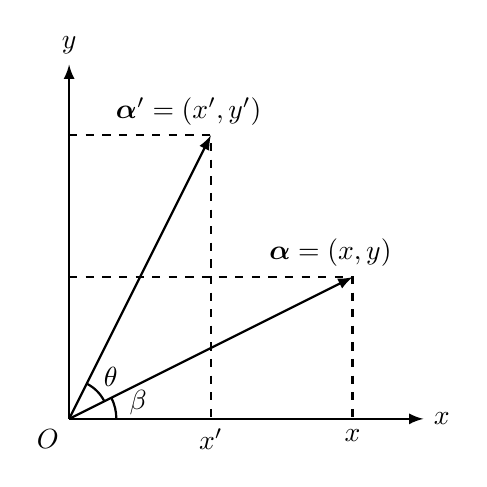
\begin{tikzpicture}[scale=1.8]
                \tikzset{>=latex, every path/.style={thick}}
                \draw (0,0) coordinate (O)
                    (1,2) coordinate (A)
                    (2,1) coordinate (B)
                    (2,0) coordinate (C);
                \draw[->] (0, 0) -- (0, 2.5)
                    node[above] {$y$};
                \draw[->] (0, 0) -- (2.5, 0)
                    node[right] {$x$};
                \draw[->] (O) -- (A)
                    node[above,xshift=-8pt] {$\boldsymbol{\alpha}'=(x',y')$};
                \draw[->] (O) -- (B)
                    node[above,xshift=-8pt] {$\boldsymbol{\alpha}=(x,y)$};
                \draw[dashed] (0,2) -- (1,2) -- (1,0) node[below] {$x'$}
                    (0,1) -- (2,1) -- (2,0) node[below] {$x$};
                \draw pic[draw,"$\theta$",angle eccentricity=1.5] {angle=B--O--A};
                \draw pic[draw,"$\beta$",angle eccentricity=1.5,angle radius=.6cm] {angle=C--O--B};
                \draw node[below left] at (O) {$O$};
            \end{tikzpicture}
        \end{center}
        \item 镜像变换(或镜面反射)--$\mathbf{R}^2$中每个向量关于过原点的直线$L$(看作镜面)相对称的变换 $\varphi$,即
        \[
        \varphi: \forall \alpha = \vec{OA} \in \mathbf{R}^2,\\
        \varphi(\alpha) = \alpha'= \vec{OB}
        \]
        \begin{center}
            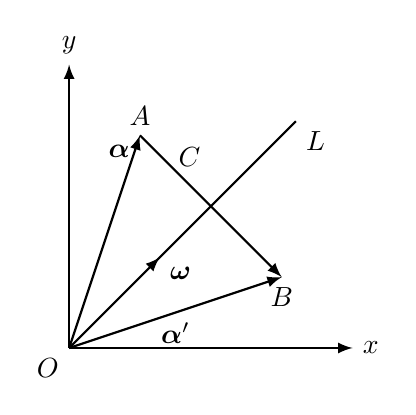
\begin{tikzpicture}[scale=1.8]
                \tikzset{>=latex, every path/.style={thick}, ->-/.style={
                    decoration={markings, mark=at position .4 with {\arrow{>}}}, postaction={decorate}
                }}
                \draw[->] (0, 0) -- (0, 2) node[above] {$y$};
                \draw[->] (0, 0) -- (2, 0) node[right] {$x$};
                \draw (0,0) coordinate (O)
                    (0.5, 1.5) coordinate (A)
                    (1.5,0.5) coordinate (B);
                \draw node[above] at (A) {$A$}
                    node[below left] at (A) {$\boldsymbol{\alpha}$}
                    node[below] at (B) {$B$};
                \draw[->] (O) -- (A);
                \draw[->] (O) -- (B)
                    node[pos=.5, below] {$\boldsymbol{\alpha}'$};
                \draw[->] (A) -- (B)
                    node[pos=.35, above=3pt] {$C$};
                \draw[->-] (O) -- (1.6, 1.6)
                    node[pos=.4, below right] {$\boldsymbol{\omega}$}
                    node[below right] {$L$};
                \draw node[below left] at (O) {$O$};
            \end{tikzpicture}
        \end{center}
        \item 三维立体空间中的投影变换也是线性变换,例如$\mathbf{R}^3$到子空间 $W=\spa((1,0,0))$ 的投影变换 $p$.
        \[
        p: \forall \alpha = (x,y,z) \in \mathbf{R}^3,\\
        p(\alpha) = \alpha'= (x,0,0)
        \]
    \end{enumerate}

\end{example}

\begin{solution}
    \begin{enumerate}
     \item 读者易根据线性映射的定义自行验证
     \item 式中的 \( x', y' \) 分别为
     \[
     x' = r \cos(\theta + \beta) = x \cos \theta - y \sin \theta,
     \]
     \[
     y' = r \sin(\theta + \beta) = x \sin \theta + y \cos \theta,
     \]
     其中 \( \beta = \langle \alpha, \vec{\mathbf{O}x} \rangle \),即
     \[
     r_{\theta}(\alpha) = r_{\theta}(x, y) = (x \cos \theta - y \sin \theta, x \sin \theta + y \cos \theta),
     \]
     于是对 \( \alpha_1 = (x_1, y_1), \alpha_2 = (x_2, y_2) \in \mathbf{R}^2 \) 和任意 \( \lambda, \mu \in \mathbf{R} \),
     \[
     r_{\theta}(\lambda \alpha_1 + \mu \alpha_2) = r_{\theta}(\lambda x_1 + \mu x_2, \lambda y_1 + \mu y_2)
     \]
     \[
     = ((\lambda x_1 + \mu x_2) \cos \theta - (\lambda y_1 + \mu y_2) \sin \theta,
     (\lambda x_1 + \mu x_2) \sin \theta + (\lambda y_1 + \mu y_2) \cos \theta)
     \]
     \[
     = \lambda (x_1 \cos \theta - y_1 \sin \theta, x_1 \sin \theta + y_1 \cos \theta)
     + \mu (x_2 \cos \theta - y_2 \sin \theta, x_2 \sin \theta + y_2 \cos \theta)
     \]
     \[
     = \lambda r_{\theta}(x_1, y_1) + \mu r_{\theta}(x_2, y_2) = \lambda r_{\theta}(\alpha_1) + \mu r_{\theta}(\alpha_2),
     \]
     故 \( r_{\theta} \) 是 \( \mathbf{R}^2 \) 上的一个线性变换.

    \item 证明涉及内积的知识,我们放在\autoref{ex:镜像变换}中讨论.
    \item 读者可以自行验证.
    \end{enumerate}

\end{solution}

除了以上的例子之外,我们也提倡读者了解其它常见的线性映射,特别是具有几何意义的例子(虽然不会直接考察,但是对理解有帮助).例如错切变换与伸缩变换的线性性,或者直接搜索仿射变换的相关内容.

\begin{example}{}{}
    写出下列映射的出发空间和到达空间,并判断其是否为线性映射:
    \begin{enumerate}
        \item $\sigma(x_1,x_2)=(x_1-x_2,x_1,x_1+x_2)$;

        \item $\sigma(x_1,x_2)=(x_1x_2,x_1+x_2)$;

        \item $\sigma(p(x))=p(x+1)-p(x),\enspace\forall p(x) \in \mathbf{R}[x]_n$;

        \item $\sigma(p(x))=p(a),\enspace\forall p(x)$,其中$a$为常数;

        \item $\sigma(\xi)=2\xi+\xi_0$,其中$\xi_0$是线性空间$V$中的一个固定向量.
    \end{enumerate}
\end{example}

\begin{solution}
    \begin{enumerate}
        \item 出发空间为 $ \mathbf{R}^2 $,到达空间为 $ \mathbf{R}^3 $. $ \sigma $ 是线性映射.

              $ \forall (x_1, x_2), (y_1, y_2) \in \mathbf{R}^2,\enspace k_1, k_2 \in \mathbf{R} $, 有
              \begin{align*}
                      & \sigma(k_1(x_1, x_2) + k_2(y_1, y_2))                                                                     \\
                  ={} & ((k_1 x_1 + k_2 y_1) - (k_1 x_2 + k_2 y_2), k_1 x_1 + k_2 y_1, (k_1 x_1 + k_2 y_1) + (k_1 x_2 + k_2 y_2)) \\
                  ={} & k_1(x_1 - x_2, x_1, x_1 + x_2) + k_2(y_1 - y_2, y_1, y_1 + y_2)                                           \\
                  ={} & k_1 \sigma(x_1, x_2) + k_2 \sigma(y_1, y_2)
              \end{align*}

        \item 出发空间为 $ \mathbf{R}^2 $,到达空间为 $ \mathbf{R}^2 $. $ \sigma $ 不是线性映射.

              $ \forall (x_1, x_2), (y_1, y_2) \in \mathbf{R}^2,\enspace k_1, k_2 \in \mathbf{R} $, 有
              \begin{align*}
                  \sigma((x_1, x_2) + (y_1, y_2))
                   & = \sigma(x_1 + y_1, x_2 + y_2)                                        \\
                   & = ((x_1 + y_1)(x_2 + y_2), ((x_1 + y_1) + (x_2 + y_2))                \\
                   & = (x_1 x_2 + x_1 y_2 + y_1 x_2 + y_1 y_2, x_1 + y_1 + x_2 + y_2)      \\
                   & = (x_1 x_2 + y_1 y_2, x_1 + y_1 + x_2 + y_2) + (x_1 y_2 + y_1 x_2, 0) \\
                   & = \sigma(x_1, x_2) + \sigma(y_1, y_2) + (x_1 y_2 + y_1 x_2, 0)        \\
                   & \neq \sigma(x_1, x_2) + \sigma(y_1, y_2)
              \end{align*}

        \item 出发空间为 $ \mathbf{R}[x]_n $,到达空间为 $ \mathbf{R}[x]_{n - 1} $. $ \sigma $ 是线性映射.

              $ \forall p_1(x), p_2(x) \in \mathbf{R}[x]_n,\enspace k_1, k_2 \in \mathbf{R} $, 有
              \begin{align*}
                      & \sigma(k_1 p_1(x) + k_2 p_2(x))                     \\
                  ={} & (k_1 p_1 + k_2 p_2)(x + 1) - (k_1 p_1 + k_2 p_2)(x) \\
                  ={} & k_1(p_1(x + 1) - p_1(x)) + k_2(p_2(x + 1) - p_2(x)) \\
                  ={} & k_1 \sigma(p_1(x)) + k_2 \sigma(p_2(x))
              \end{align*}

        \item 出发空间为 $ \mathbf{R}[x] $,到达空间为 $ \mathbf{R}[x] $. $ \sigma $ 是线性映射.

              $ \forall p_1(x), p_2(x) \in \mathbf{R}[x],\enspace k_1, k_2 \in \mathbf{R} $, 有
              \begin{align*}
                      & \sigma(k_1 p_1(x) + k_2 p_2(x))         \\
                  ={} & (k_1 p_1 + k_2 p_2)(a)                  \\
                  ={} & k_1 p_1(a) + k_2 p_2(a)                 \\
                  ={} & k_1 \sigma(p_1(x)) + k_2 \sigma(p_2(x))
              \end{align*}

        \item 出发空间为 $ V $,到达空间为 $ V $. 当 $ \xi_0 = \vec{0} $ 时, $ \sigma(\xi) = 2 \xi $ 是线性映射.

              $ \forall \xi_1, \xi_2 \in V $, 有
              \begin{align*}
                  \sigma(\xi_1 + \xi_2) & = 2(\xi_1 + \xi_2)              \\
                                        & = 2 \xi_1 + 2 \xi_2             \\
                                        & = \sigma(\xi_1) + \sigma(\xi_2)
              \end{align*}

              当 $ \xi_0 \neq \vec{0} $ 时, $ \sigma $ 不是线性映射.

              $ \forall \xi_1, \xi_2 \in V $, 有
              \begin{align*}
                  \sigma(\xi_1 + \xi_2) & = 2(\xi_1 + \xi_2) + \xi_0              \\
                                        & = 2 \xi_1 + 2 \xi_2 + \xi_0             \\
                                        & = \sigma(\xi_1) + \sigma(\xi_2) - \xi_0 \\
                                        & \neq \sigma(\xi_1) + \sigma(\xi_2)
              \end{align*}
    \end{enumerate}
\end{solution}

\subsection{线性映射的基本运算}

我们在之前的学习中已经了解,连续函数关于函数的加法数乘运算可以构成线性空间,事实上线性映射可以视为特殊的函数,因此我们希望在本节讨论怎样的运算定义能使其构成线性空间,除此之外也介绍线性映射乘法(即复合)和逆运算.

我们需要首先说明一个记号,我们把线性空间$V_1(\mathbf{F})$到$V_2(\mathbf{F})$的所有线性映射组成的集合记作$\mathcal{L}(V_1,V_2)$(类似于将定义在$[a,b]$上取值于实数集的连续函数全体记为$C[a,b]$). 如果是出发空间与到达空间均为$V$的线性变换全体,我们可以简记为$\mathcal{L}(V)$. 我们希望在该集合上定义线性空间,于是需要定义其中元素(线性映射)的加法和数乘运算:
\begin{definition}{}{}
    设$\sigma,\tau\in \mathcal{L}(V_1,V_2)$,规定$\sigma$与$\tau$之和及$\lambda$与$\sigma$的数乘$\lambda\sigma$分别为
    \begin{gather*}
        (\sigma+\tau)(\alpha)=\sigma(\alpha)+\tau(\alpha),\enspace\forall\alpha\in V_1 \\
        (\lambda\sigma)(\alpha)=\lambda(\sigma(\alpha)),\enspace\forall\alpha\in V_1
    \end{gather*}
\end{definition}

不难验证,这样定义的线性映射加法和数乘的结果仍然是线性映射:
\begin{proof}
\begin{enumerate}
    \item 首先证明加法,直接验证即可:
    \begin{align*}
        (\sigma + \tau)(\lambda_1 \alpha_1 + \lambda_2 \alpha_2) & = \sigma(\lambda_1 \alpha_1 + \lambda_2 \alpha_2) + \tau(\lambda_1 \alpha_1 + \lambda_2 \alpha_2) \\
        & = \lambda_1 \sigma(\alpha_1) + \lambda_2 \sigma(\alpha_2) + \lambda_1 \tau(\alpha_1) + \lambda_2 \tau(\alpha_2) \\
        & = \lambda_1 (\sigma(\alpha_1) + \tau(\alpha_1)) + \lambda_2 (\sigma(\alpha_2) + \tau(\alpha_2)) \\
        &= \lambda_1 (\sigma+\tau)(\alpha_1) + \lambda_2 (\sigma+\tau)(\alpha_2).
    \end{align*}

    \item 再证明数乘,同样直接验证即可:
    \begin{align*}
        (\lambda \sigma)(\lambda_1 \alpha_1 + \lambda_2 \alpha_2) & = \lambda \sigma(\lambda_1 \alpha_1 + \lambda_2 \alpha_2) \\
        & = \lambda (\lambda_1 \sigma(\alpha_1) + \lambda_2 \sigma(\alpha_2)) \\
        & = \lambda_1 (\lambda \sigma(\alpha_1)) + \lambda_2 (\lambda \sigma(\alpha_2)) \\
        & = \lambda_1 (\lambda \sigma)(\alpha_1) + \lambda_2 (\lambda \sigma)(\alpha_2).
    \end{align*}
\end{enumerate}
\end{proof}

进一步地,线性空间 $V_1(\mathbf{F})$ 到 $V_2(\mathbf{F})$ 的所有线性映射 $\mathcal{L}(V_1,V_2)$ 关于上面定义的加法和数乘构成线性空间:

\begin{theorem}{}{线性映射全体构成线性空间}
    $\mathcal{L}(V_1,V_2)$与上述定义的线性映射加法和数乘构成域$\mathbf{F}$上的线性空间.
\end{theorem}

实际上,前面我们证明的线性映射加法和数乘的结果仍然是线性映射,就是线性映射的加法和数乘的封闭性,因此我们只需证明线性映射的加法和数乘满足线性空间的 8 条性质即可. 事实上这是非常显然的,我们只需注意 $\mathcal{L}(V_1,V_2)$ 中的零元就是零映射 $\theta$(将 $V_1$ 中的任意元素都映射到 $V_2$ 中的零元)即可,因此我们不再赘述.

下面讨论线性映射的其它运算. 首先是复合运算. 设$\sigma \in \mathcal{L}(V_1,V_2),\enspace\tau \in \mathcal{L}(V_2,V_3)$,则$\tau\sigma$是$\mathcal{L}(V_1,V_3)$中的元素,且$\tau\sigma(\alpha)=\tau(\sigma(\alpha)),\enspace\forall \alpha \in V_1$.

\begin{theorem}{}{复合映射是线性映射}
    上述定义的映射 $\tau\sigma$ 是线性映射.
\end{theorem}

注意:在上述定义中一定注意$\sigma$和$\tau$的顺序,我们需要先使用$\sigma$将$V_1$中的元素映射到$V_2$,然后再用外层的$\tau$将这个结果映射到$V_3$. 此外,有时也会将复合映射记作$\tau \circ \sigma$(一般是为了强调这是复合运算),这里为了简化记号直接使用$\tau\sigma$.

接下来定义线性映射的逆运算,也就是定义逆映射,事实上与反函数的定义类似. 设 $\sigma \in \mathcal{L}(V_1,V_2)$. 若存在 $\tau \in \mathcal{L}(V_2,V_1)$ 使得 $\sigma \tau = I_{V_2}$ 且 $\tau \sigma = I_{V_1}$,则称 $\sigma$\term{可逆}\index{ni!ke@可逆 (invertible)},并称 $\tau$ 为 $\sigma$ 的逆映射\index{ni!yingshe@映射 (inverse map)}. 其中 $I_{V_1}$ 和 $I_{V_2}$ 分别是 $V_1$ 和 $V_2$ 上的恒等映射,即 $I_{V_i}(\alpha)=\alpha,\enspace \forall \alpha \in V_i,\ i = 1, 2$.

\begin{theorem}{}{逆映射是线性映射}
    上述定义的逆映射 $\sigma^{-1}$ 为线性映射.
\end{theorem}

\autoref{thm:复合映射是线性映射}和\autoref{thm:逆映射是线性映射}的证明是非常基本的,在阅读详细的证明之前,读者可以先自行尝试,如果不会证明则说明对于线性空间和线性映射的定义熟悉程度仍需提高,因为这里的证明都只需要机械地套用定义.

\begin{proof}
\begin{enumerate}
    \item 如果 $\sigma_1$ 和 $\sigma_2$ 分别是线性空间 $V_1(F)$ 到 $V_2(F)$ 和 $V_2(F)$ 到 $V_3(F)$ 的线性映射,那么
    \begin{align*}
        (\sigma_2 \circ \sigma_1)(\lambda \alpha  + \mu \beta) & = \sigma_2(\sigma_1(\lambda \alpha  + \mu \beta)) \\
        & = \sigma_2(\lambda (\sigma_1(\alpha))) + \mu_1(\sigma_1(\beta)) \\
        & = \lambda (\sigma_2(\sigma_1)(\alpha)) + \mu (\sigma_2(\sigma_1)(\beta)),
    \end{align*}
    所以 $\sigma_2\sigma_1$ 是 $V_1$ 到 $V_3$ 的线性映射.

    \item 如果可逆线性映射 $\sigma: V_1 \to V_2$ 的逆映射为 $\sigma^{-1}: V_2 \to V_1$,那么
    \[
    \sigma^{-1} \circ \sigma = I_{V_1}, \quad \text{且} \quad \sigma \circ \sigma^{-1} = I_{V_2},
    \]
    于是对于$ \forall \ \beta_1,\beta_2 \in V_2$和任意的标量 $\lambda_1, \lambda_2 \in F$,有
    \begin{align*}
        \sigma^{-1}(\lambda_1 \beta_1 + \lambda_2 \beta_2) & = \sigma^{-1}\left[ \lambda_1(\sigma \sigma^{-1})(\beta_1)+\lambda_2(\sigma \sigma^{-1})(\beta_2)\right] \\
        &= \sigma^{-1}(\lambda_1 \sigma(\sigma^{-1}(\beta_1)) + \lambda_2 \sigma(\sigma^{-1}(\beta_2))) \\
        & = \lambda_1 \sigma^{-1}(\beta_1) + \lambda_2 \sigma^{-1}(\beta_2),
    \end{align*}
    所以 $\sigma^{-1}$ 是线性的.
\end{enumerate}
\end{proof}

除此之外,关于线性映射的复合,我们还有结合律,即 $\tau(\sigma\eta) = (\tau\sigma)\eta$,这是显然的,因为
\[\tau(\sigma\eta)(\alpha) = \tau((\sigma\eta)(\alpha)) = \tau(\sigma(\eta(\alpha))) = (\tau\sigma)(\eta(\alpha)) = (\tau\sigma)\eta(\alpha).\]
这与普通函数的复合运算满足结合律没有任何区别.

\section{线性映射的像与核}

我们在之前的讨论中已经了解了线性映射的定义与运算,接下来我们需要关心的问题是:定义出的线性映射能将出发空间完整映射到到达空间吗,还是到达空间中有些向量无法被映到?线性映射是否可以是单射?单射的充要条件又是什么?这与我们研究一般的映射的思路是类似的. 因此我们希望在本节讨论线性映射的像和核.
\begin{definition}{}{}
    设$\sigma$是线性空间$V_1(\mathbf{F})$到$V_2(\mathbf{F})$的线性映射. $V_1$的所有元素在$\sigma$下的像组成的集合
    \[\sigma(V_1)=\{\beta \mid \beta=\sigma(\alpha),\enspace \alpha \in V_1\}\]
    称为$\sigma$的\term{像}(或\term{值域})\index{xiang@像 (image), 值域 (range)},记作$\im \sigma$,或记作 $\operatorname{range}\sigma$.

    $V_2$的零元$0_2$在$\sigma$下的完全原像
    \[\sigma^{-1}(0_2)=\{\alpha \mid \sigma(\alpha)=0_2,\enspace \alpha \in V_1\}\]
    称为$\sigma$的\term{核}(或\term{零空间})\index{he@核 (kernel), 零空间 (null space)},记作$\ker \sigma$,或记作 $\operatorname{null}\sigma$.
\end{definition}

关于像与核的定义,我们需要强调以下几点:
\begin{enumerate}
    \item 实际上,像空间的定义就类似于函数的值域,核空间可以视为到达空间中0的原像集合,因此理解起来是很简单的;

    \item 注意线性映射的像和核分别是$V_2$和$V_1$的子空间. 同样地,若$W_1$和$W_2$分别是$V_1$和$V_2$的子空间,则$\sigma(W_1)$和$\sigma^{-1}(W_2)$也分别是$V_2$和$V_1$的子空间.我们在此只给出前者的证明,后者我们作为习题留给读者,实际上都非常简单,只是为读者熟悉定义而在此处提及.
          \begin{proof}
              首先我们证明像空间是$V_2$的子空间. 设$\beta_1,\beta_2\in \sigma(V_1)$,则存在$\alpha_1,\alpha_2\in V_1$使得$\beta_1=\sigma(\alpha_1),\beta_2=\sigma(\alpha_2)$,于是
              \[\beta_1+\beta_2=\sigma(\alpha_1)+\sigma(\alpha_2)=\sigma(\alpha_1+\alpha_2)\in \sigma(V_1),\]
              \[\lambda\beta_1=\lambda\sigma(\alpha_1)=\sigma(\lambda\alpha_1)\in \sigma(V_1),\]
              因此$\sigma(V_1)$是$V_2$的子空间.

              接下来我们证明核空间是$V_1$的子空间. 设$\alpha_1,\alpha_2\in \sigma^{-1}(0_2)$,则$\sigma(\alpha_1)=\sigma(\alpha_2)=0_2$,于是
              \[\sigma(\alpha_1+\alpha_2)=\sigma(\alpha_1)+\sigma(\alpha_2)=0_2+0_2=0_2,\]
              \[\lambda\sigma(\alpha_1)=\sigma(\lambda\alpha_1)=0_2,\]
              因此$\sigma^{-1}(0_2)$是$V_1$的子空间.
          \end{proof}
\end{enumerate}

接下来我们要讨论如何计算线性映射的像与核,这在考试中非常常见,请务必牢记,无论线性映射有多么复杂多么抽象,基本的方法都是:
\begin{enumerate}
    \item 设出发空间的一组基为$B=\{\alpha_1,\alpha_2,\ldots,\alpha_n\}$,则像空间
          \[\im \sigma=\sigma(V_1)=\spa(\sigma(\alpha_1),\sigma(\alpha_2),\ldots,\sigma(\alpha_n)).\]
          即线性映射在出发空间一组基下的像的线性扩张,解答时写出极大线性无关组然后扩张即可;

          当然读者可能质疑其合理性,因为与定义不完全一致. 我们可以证明这一方法是合理的,即线性映射在出发空间一组基下像的线性扩张就是其像空间.

          \begin{proof}
              首先我们知道$\sigma(V_1)$包含$\sigma(\alpha_1),\sigma(\alpha_2),\ldots,\sigma(\alpha_n)$,并且是$V_2$的子空间. 又根据\autoref{thm:线性扩张构造子空间},$\sigma(V_1)$是包含$\sigma(\alpha_1),\sigma(\alpha_2),\ldots,\sigma(\alpha_n)$的最小子空间,因此我们可以得到$\spa(\sigma(\alpha_1),\sigma(\alpha_2),\ldots,\sigma(\alpha_n))\subseteq\sigma(V_1)$.

              接下来证明另一半包含. 根据线性扩张定义可知只需证$V_1$中任意元素的像都可以被$\sigma(\alpha_1),\sigma(\alpha_2),\ldots,\sigma(\alpha_n)$线性表示. 任取$\alpha\in V_1$,则$\alpha$可由$V_1$一组基$\{\alpha_1,\alpha_2,\ldots,\alpha_n\}$线性表示为$\alpha=\lambda_1\alpha_1+\lambda_2\alpha_2+\cdots+\lambda_n\alpha_n$,于是,
              \[\sigma(\alpha)=\sigma(\lambda_1\alpha_1+\lambda_2\alpha_2+\cdots+\lambda_n\alpha_n)=\lambda_1\sigma(\alpha_1)+\lambda_2\sigma(\alpha_2)+\cdots+\lambda_n\sigma(\alpha_n)\]
              即$\sigma(\alpha)$可由$\sigma(\alpha_1),\sigma(\alpha_2),\ldots,\sigma(\alpha_n)$线性表示,即出发空间任意向量在$\sigma$下的像都可以由$\sigma(\alpha_1),\sigma(\alpha_2),\ldots,\sigma(\alpha_n)$线性表示,因此$\sigma(V_1)\subseteq\spa(\sigma(\alpha_1),\sigma(\alpha_2),\ldots,\sigma(\alpha_n))$.
          \end{proof}

    \item 核空间可以直接利用定义令$\sigma(\alpha)=0$,利用解线性方程组得到解集即为结果,注意也许表示为线性扩张的形式.
\end{enumerate}

\begin{example}{}{}
    已知$\mathbf{R}^3$到$\mathbf{R}^2$的映射$\sigma$为$\sigma(x_1,x_2,x_3)^{\color{lightgray}\mathrm{T}}=(x_1+x_2,x_2-x_3)^{\color{lightgray}\mathrm{T}}$,求$\sigma$的像和核.
\end{example}
注:这里需要对记号进行一个澄清,事实上 $\mathbf{R}^n$ 空间中的向量都应当是列向量,但为了节省空间,一些教材在描述映射的情形下会写成行向量的形式. 但笔者认为线性映射相关的地方行和列的混乱容易导致一些困惑,为此,笔者有时会在向量的右上角加上一个浅色的转置 $({}^{\color{gray}\mathrm{T}})$ 以代表它是列向量.

\begin{solution}
    \begin{itemize}
        \item 首先求像空间. 取出发空间$\mathbf{R}^3$的一组基$B=\{(1,0,0)^{\color{lightgray}\mathrm{T}},(0,1,0)^{\color{lightgray}\mathrm{T}},(0,0,1)^{\color{lightgray}\mathrm{T}}\}$,则
        \begin{align*}
            \im \sigma &=\sigma(\mathbf{R}^3) = \spa(
                \sigma(1,0,0)^{\color{lightgray}\mathrm{T}},
                \sigma(0,1,0)^{\color{lightgray}\mathrm{T}},
                \sigma(0,0,1)^{\color{lightgray}\mathrm{T}}
                 ) \\
            &=\spa(
                (1,0)^{\color{lightgray}\mathrm{T}},
                (1,1)^{\color{lightgray}\mathrm{T}},
                (0,-1)^{\color{lightgray}\mathrm{T}}
                )
        \end{align*}
        根据求解极大线性无关组的方法(或者这么简单的情况瞪眼法也可以)得到像空间
        $\im \sigma=\spa((1,0)^{\color{lightgray}\mathrm{T}},(0,-1)^{\color{lightgray}\mathrm{T}})=\mathbf{R}^2$.

        \item 接下来求解核空间. 设$\sigma(\alpha)=0$,其中$\alpha=(x_1,x_2,x_3)^{\color{lightgray}\mathrm{T}}$,即$\sigma(x_1,x_2,x_3)^{\color{lightgray}\mathrm{T}}=(x_1+x_2,x_2-x_3)^{\color{lightgray}\mathrm{T}}=(0,0)$,解得解向量为$k(-1,1,1)^{\color{lightgray}\mathrm{T}},\enspace k\in\mathbf{R}$,写成线性扩张的形式为$\spa((-1,1,1)^{\color{lightgray}\mathrm{T}})$.
    \end{itemize}
\end{solution}

下面我们也给出另一种求像空间的方法,但是为了防止读者混淆这一方法和之后线性映射矩阵表示的方法,希望读者能按照笔者首先介绍的方法求解.
\begin{solution}\label{ex:线性映射的像空间求解2}
    \begin{align*}
        \sigma(x_1, x_2, x_3)^{\color{lightgray}\mathrm{T}} &= (x_1 + x_2, x_2 - x_3)^{\color{lightgray}\mathrm{T}}\\
        &= x_1(1, 0)^{\color{lightgray}\mathrm{T}} + x_2(1, 1)^{\color{lightgray}\mathrm{T}} + x_3(0, -1)^{\color{lightgray}\mathrm{T}}
    \end{align*}
    记 $\beta_1 = (1, 0)^{\color{lightgray}\mathrm{T}}, \beta_2 = (1, 1)^{\color{lightgray}\mathrm{T}}, \beta_3 = (0, -1)^{\color{lightgray}\mathrm{T}}$,则 $\sigma(x_1, x_2, x_3)^{\color{lightgray}\mathrm{T}} = x_1 \beta_1 + x_2 \beta_2 + x_3 \beta_3$,所以 $\sigma(\mathbf{R}^3) = \spa\{\beta_1, \beta_2, \beta_3\} = \spa \{\beta_1, \beta_2\}=\mathbf{R}^2$.
\end{solution}


事实上,研究一般映射我们会很在意映射是否为单射或满射. 是否为满射通过我们介绍的求解像空间的方法是很好判断的,但单射似乎并不能直接利用像空间或者核空间直接判断,但我们只需稍作转化就可以发现单射和核空间有着密不可分的联系:
\begin{theorem}{}{单射与核空间}
    线性映射$\sigma$是单射当且仅当$\ker \sigma=\{0\}$.
\end{theorem}
这个定理告诉我们,线性映射是单射和0的逆像只有0是等价的. 这一结论也是非常强的,因为我们知道一般的函数是不满足这一结论的,例如$f(x)=x^2$,虽然只有$f(0)=0$,但在$\mathbf{R}$上显然不是单射. 这一定理证明非常简单,希望读者掌握:

\begin{proof}
    首先我们证明$\sigma$是单射时$\ker\sigma=\{0\}$. 事实上$\sigma$是单射意味着任意到达空间中的元素的逆象唯一,又线性映射必须满足$\sigma(0)=0$,则0的逆象唯一为0是显然的.

    接下来我们证明$\ker \sigma=\{0\}$时$\sigma$是单射. 事实上,$\sigma(\alpha)=\sigma(\beta)$等价于$\sigma(\alpha)-\sigma(\beta)=0$,即$\sigma(\alpha-\beta)=0$,由于$\ker \sigma=\{0\}$,因此$\alpha-\beta=0$,即$\alpha=\beta$,因此$\sigma$是单射.
\end{proof}

\section{线性映射的确定}

我们知道,两个函数相等当且仅当它们的定义域相等且对于任意定义域内的元素,它们的函数值相等. 线性映射则有更好的性质,即有限维空间上的线性映射可以被基上的像唯一确定,即
\begin{theorem}{}{线性映射唯一确定}
    已知线性映射$\sigma,\tau\in \mathcal{L}(V_1,V_2)$,且有$V_1$的基$B=\{\alpha_1,\alpha_2,\ldots,\alpha_n\}$. 若$\sigma(\alpha_i)=\tau(\alpha_i),\enspace\forall \alpha_i \in B$,则有$\sigma=\tau$.
\end{theorem}
即映射在一组基上的像确定了,则映射是唯一的. 证明非常简单:

\begin{proof}
    实际上我们只需证明$\sigma(\alpha)=\tau(\alpha),\enspace\forall \alpha \in V_1$即可,因为这就是一般映射相等的条件. 事实上,任取$\alpha \in V_1$,则$\alpha$可由$B$线性表示为$\alpha=\lambda_1\alpha_1+\lambda_2\alpha_2+\cdots+\lambda_n\alpha_n$,于是
    \begin{gather*}
        \sigma(\alpha)=\sigma(\lambda_1\alpha_1+\lambda_2\alpha_2+\cdots+\lambda_n\alpha_n)=\lambda_1\sigma(\alpha_1)+\lambda_2\sigma(\alpha_2)+\cdots+\lambda_n\sigma(\alpha_n) \\
        \tau(\alpha)=\tau(\lambda_1\alpha_1+\lambda_2\alpha_2+\cdots+\lambda_n\alpha_n)=\lambda_1\tau(\alpha_1)+\lambda_2\tau(\alpha_2)+\cdots+\lambda_n\tau(\alpha_n)
    \end{gather*}
    由于$\sigma(\alpha_i)=\tau(\alpha_i),\enspace\forall \alpha_i \in B$,因此$\sigma(\alpha)=\tau(\alpha)$,即$\sigma=\tau$.
\end{proof}

事实上这与之前证明求解像空间的方法合理性(即证线性映射在一组基上的像的线性扩张就是线性映射的像空间)是完全相通的. 这里也蕴含了一个数学的基本想法. 我们发现线性映射比一般的函数要求更高,因为它要求了两个运算性质,我们说这里构成线性映射的条件比构成一般函数的条件``更强''. 更强的要求必然带来更美妙的结果,例如线性映射可被基上的像唯一确定,而一般函数则不存在这样的性质. 抑或是未来如果有同学学习复变函数时,那时我们研究的``全纯函数''比数学分析中常见的连续函数要求更强,因此会有大量在数学分析中无法想象的非常漂亮的结果. 值得一提的是,复变函数这样美妙的结果直接带来了\nameref{thm:代数学基本定理}的非常简便的证明,这在数学史上是非常重要的里程碑.

\begin{theorem}{}{线性映射构造}
    设$B=\{\alpha_1,\alpha_2,\ldots,\alpha_n\}$是$V_1$的基,$S=\{\beta_1,\beta_2,\ldots,\beta_n\}$是$V_2$中任意$n$个向量,则存在唯一的$\sigma\in \mathcal{L}(V_1,V_2)$使得$\sigma(\alpha_i)=\beta_i,\enspace i=1,2,\ldots,n$.
\end{theorem}

\begin{proof}
这一定理的证明也是简单的,只需先定义出这个映射. $\forall \alpha \in V_1$,则$\alpha$可由$B$线性表示为$\alpha=\lambda_1\alpha_1+\lambda_2\alpha_2+\cdots+\lambda_n\alpha_n$,于是定义
\[\sigma(\alpha)=\sigma(\lambda_1\alpha_1+\lambda_2\alpha_2+\cdots+\lambda_n\alpha_n)=\lambda_1\beta_1+\lambda_2\beta_2+\cdots+\lambda_n\beta_n\]
即可满足条件,因为我们可以验证这是线性映射:

\[
\forall \enspace \xi_1, \xi_2 \in V_1, \lambda_1, \lambda_2 \in F
\]
\[
\begin{cases}
    \xi_1 = x_1\alpha_1+x_2\alpha_2+\cdots+x_n\alpha_n,\\
    \xi_2 = y_1\alpha_1+y_2\alpha_2+\cdots+y_n\alpha_n
\end{cases}
\]
\begin{align*}
\sigma(\lambda_1 \xi_1 + \lambda_2 \xi_2) &= \sigma(\lambda_1(x_1\alpha_1+x_2\alpha_2+\cdots+x_n\alpha_n) + \lambda_2(y_1\alpha_1+y_2\alpha_2+\cdots+y_n\alpha_n))\\
&= \lambda_1(x_1\beta_1+x_2\beta_2+\cdots+x_n\beta_n) + \lambda_2(y_1\beta_1+y_2\beta_2+\cdots+y_n\beta_n)\\
&= \lambda_1\sigma(\xi_1) + \lambda_2\sigma(\xi_2)
\end{align*}

并且唯一性在\autoref{thm:线性映射唯一确定} 中已经说明. 实际上对于初学而言难点在于定义,实际上证明后会发现这一定义太自然了,就是向着线性性定义的,因此很多构造不需要太复杂的想法,自然的、满足要求的是最好的.
\end{proof}
最后我们讨论一个初学时容易困惑的问题,如下例所示:
\begin{example}{}{线性映射判断1}
    是否存在$\mathbf{R}^2$到$\mathbf{R}^3$的线性映射$\sigma$使得$\sigma(1,0)^{\color{lightgray}\mathrm{T}}=(1,0,0)^{\color{lightgray}\mathrm{T}},\enspace\sigma(0,1)^{\color{lightgray}\mathrm{T}}=(0,1,0)^{\color{lightgray}\mathrm{T}},\enspace\sigma(1,1)^{\color{lightgray}\mathrm{T}}=(0,0,1)^{\color{lightgray}\mathrm{T}}$?
\end{example}

初学时感到困难是因为不能熟练应用线性映射的各类性质,找不到映射定义也不敢下结论不存在,或者发现必要条件都满足了却不敢构造. 我们这里给出几个解决策略:
\begin{enumerate}
    \item \label{item:5:线性映射判断1:1}
          根据\autoref{thm:线性映射零元性质} 可知,如果我们发现题目给定的条件无法满足将出发空间零元映射至到达空间零元则一定不是线性映射;

    \item \label{item:5:线性映射判断1:2}
          根据\autoref{thm:线性映射保相关性} 可知,如果我们发现映射将线性相关的向量组映射到了线性无关向量组,则一定不是线性映射;

    \item \label{item:5:线性映射判断1:3}
          不存在从低维线性空间到高维线性空间的满射,原因是简单的:取低维出发空间的一组基$B=\{\alpha_1,\alpha_2,\ldots,\alpha_m\}$,则基下的像的线性扩张$\spa(\sigma(\alpha_1),\sigma(\alpha_2),\ldots,\sigma(\alpha_m))$就是像空间. 我们取高维到达空间的一组基$B_2=\{\beta_1,\beta_2,\ldots,\beta_n\}$,则由于维数更高有$n>m$. 由于$\sigma$是满射,因此$\sigma(\alpha_1),\sigma(\alpha_2),\ldots,\sigma(\alpha_m)$可以线性表示出$B_2$中任意向量,根据\autoref{thm:线性表示} 可知(这是长的向量可以被短的向量线性表示),向量组$B_2$线性相关,但我们知道这是一组基,因此矛盾!

          这一性质在下一讲介绍了线性映射基本定理后会有更简单的证明,但此处的证明也是很重要的,体现了\autoref{thm:线性表示} 作为源泉定理的重要性.

    \item 如果题目给定的映射不违反上述线性映射的必要条件,那我们可以按照\autoref{thm:线性映射构造} 构造出相应的映射.
\end{enumerate}

根据上面的描述,我们发现 \ref*{item:5:线性映射判断1:1} 中的映射定义违反了明显违反了不能是从低维到高维满射的条件. 实际上,$\sigma$也将线性相关的向量组映射到了线性无关的向量组,并且根据定义,$\sigma(0)=\sigma((1,0)^{\color{lightgray}\mathrm{T}}+(0,1)^{\color{lightgray}\mathrm{T}}-(1,1)^{\color{lightgray}\mathrm{T}})=(1,1,-1)$,因此所有的必要条件都被违反了,因此这一映射一定不是线性映射. 事实上这一例子也表明很多时候三个必要条件可能是同时违反的,因为它们都是由基本的线性映射和线性相关性质推导而来,并非完全独立的判据.

我们还需强调的是,如果\autoref{thm:线性映射构造} 前提成立,即题目给我们的是一组基下的像,则一定不会违反上述三个必要条件. 对于条件 \ref*{ex:线性映射判断1},给定一组基$\alpha_1,\ldots,\alpha_n$,我们要凑出$\sigma(0)$只能通过$\sigma(0)=\sigma(0\alpha_1+\cdots+0\alpha_n)=0\sigma(\alpha_1)+\cdots+0\sigma(\alpha_n)=0$,因此不可能违反  \ref*{item:5:线性映射判断1:1}. 对于 \ref*{item:5:线性映射判断1:2},我们给定的是基,因此不存在将线性相关向量组映射到线性无关向量组的情况. 对于 \ref*{item:5:线性映射判断1:3},如果题目给出的是低维到高维的映射,由于我们只给出了低维出发空间的基下的像,这些像不可能张成整个高维到达空间(原理和$n-1$个向量无法张成$n$维空间一致),因此也不可能违反 \ref*{item:5:线性映射判断1:3},因此\autoref{thm:线性映射构造} 并不与我们的必要条件相矛盾,相反,如果题目给出的是一组基下的像,我们就可以毫无顾虑地说映射一定存在.

最后我们再看一个例子来练习我们上面的策略:
\begin{example}{}{线性映射判断2}
    是否存在$\mathbf{R}^3$到$\mathbf{R}^2$的线性映射$\sigma$使得$\sigma(1,-1,1)^{\color{lightgray}\mathrm{T}}=(1,0)^{\color{lightgray}\mathrm{T}},\enspace\sigma(1,1,1)^{\color{lightgray}\mathrm{T}}=(0,1)^{\color{lightgray}\mathrm{T}}$?
\end{example}

\begin{solution}
    事实上这里的定义完全不违反上述的必要条件,因此我们考虑证明这一线性映射存在. 根据\autoref{thm:线性映射构造},我们考虑构造出$\sigma$在一组基(我们取自然基)下的像,然后我们就可以根据\autoref*{thm:线性映射构造} 知道这一映射一定存在.

    实际上,根据提给条件我们有
    \begin{gather*}
        \sigma(1,-1,1)^{\color{lightgray}\mathrm{T}}
        =\sigma(e_1-e_2+e_3)
        =\sigma(e_1)-\sigma(e_2)+\sigma(e_3)
        =(1,0)^{\color{lightgray}\mathrm{T}} \\
        \sigma(1,1,1)^{\color{lightgray}\mathrm{T}}
        =\sigma(e_1+e_2+e_3)
        =\sigma(e_1)+\sigma(e_2)+\sigma(e_3)
        =(0,1)^{\color{lightgray}\mathrm{T}}
    \end{gather*}
    我们希望解出$\sigma(e_1),\sigma(e_2),\sigma(e_3)$,这样就可以直接根据\autoref*{thm:线性映射构造} 构造出这一线性映射. 但这一方程组只有2个方程却有三个未知量. 事实上我们可以任意定义$\sigma(e_3)=(0,0)$,然后解方程组得到
    \[\sigma(e_1)=\dfrac{1}{2} (1,1)^{\color{lightgray}\mathrm{T}},\enspace \sigma(e_2)=\dfrac{1}{2} (-1,1)^{\color{lightgray}\mathrm{T}}\]
    又由$\sigma(e_3)=(0,0)^{\color{lightgray}\mathrm{T}}$,根据\autoref*{thm:线性映射构造},满足题目条件的线性映射存在.
\end{solution}
需要注意的是题目中$\sigma(e_3)$不一定要定义为$(0,0)$,这样只是为了计算方便,事实上定义成任何值都可以得到$\sigma$在一组基下的像,从而根据\autoref*{thm:线性映射构造} 得到这一线性映射存在. 如果题目要求我们写出映射也并不复杂,根据我们在\autoref*{thm:线性映射构造} 中的构造方法,我们可以写出$\forall\alpha=(x,y,z)=xe_1+ye_2+ze_3$,
\[
    \sigma(\alpha)
    =\sigma(xe_1+ye_2+ze_3)
    =x\sigma(e_1)+y\sigma(e_2)+z\sigma(e_3)
    =\dfrac{1}{2} (x-y,x+y)^{\color{lightgray}\mathrm{T}}
\]
符合题目条件. 事实上根据$\sigma(e_3)$定义的不唯一,我们可以得到不同的线性映射,这里只是给出一种可能的解.

\section{线性映射基本定理}

\subsection{线性映射基本定理的陈述与证明}

本节将要介绍的定理是线性代数最重要的定理之一,因其重要性也被冠以(有限维线性空间)线性映射基本定理的名号. 为了介绍这一定理,我们需要首先引入一个概念:线性映射的秩. 在线性映射像求解的讨论中我们有$\im \sigma=\sigma(V_1)=\spa(\sigma(\alpha_1),\sigma(\alpha_2),\ldots,\sigma(\alpha_n))$. 我们基于此定义线性映射的秩:
\begin{definition}{}{}
    设$\sigma\in \mathcal{L}(V_1,V_2)$,如果$\sigma(V_1)$是$V_2$的有限维子空间,则$\sigma(V_1)$的维数称为$\sigma$的秩,记作$r(\sigma)$,即$r(\sigma)=\dim \sigma(V_1)$.
\end{definition}

这一定义是平凡的,简单理解线性映射的秩即为线性映射像空间的维数. 基于这一定理我们便可以介绍本节的核心定理:

\begin{theorem}{线性映射基本定理}{线性映射基本定理}
    设$\sigma \in \mathcal{L}(V_1,V_2)$,若$\dim V_1=n$,则
    \[r(\sigma)+\dim\ker\sigma=n.\]
\end{theorem}
简而言之,这一定理表明:线性映射的秩(或者说线性映射像空间维数)与核空间维数之和等于出发空间的维数. 这一定理的证明非常重要,在之后的很多讨论中还会用到这一思想,因此我们给出详细的证明并阐述其中的思想:

\begin{proof}
    证明的思路和\nameref{thm:线性空间维数公式}的证明思路类似,即``设小扩大''.

    我们设$\dim\ker\sigma=k$,并设$\ker\sigma$的一组基为$\alpha_1,\alpha_2,\ldots,\alpha_k$. 我们将其扩充为$V_1$的一组基,记为$\alpha_1,\alpha_2,\ldots,\alpha_k,\alpha_{k+1},\ldots,\alpha_n$.

    根据定理要证明的等式和前述假设,我们只需证$r(\sigma)=n-k$,即证明像空间维数为$n-k$. 我们知道像空间为$\spa(\sigma(\alpha_1),\sigma(\alpha_2),\ldots,\sigma(\alpha_n))$,其中根据我们的假设,$\sigma(\alpha_1)=\sigma(\alpha_2)=\cdots=\sigma(\alpha_k)=0$(因为它们是核空间的基),因此像空间为$\spa(\sigma(\alpha_{k+1}),\ldots,\sigma(\alpha_n))$. 我们只需证明这一向量组是线性无关的即可,因为这样这$n-k$个向量就可以构成像空间的一组基,从而证明了$r(\sigma)=n-k$.

    我们设$c_{k+1}\sigma(\alpha_{k+1})+\cdots+c_n\sigma(\alpha_n)=0$,即
    \[\sigma(c_{k+1}\alpha_{k+1}+\cdots+c_n\alpha_n)=0\]
    故$c_{k+1}\alpha_{k+1}+\cdots+c_n\alpha_n \in \ker\sigma$,因此可以被$\alpha_1,\alpha_2,\ldots,\alpha_k$线性表示. 于是有
    \[c_{k+1}\alpha_{k+1}+\cdots+c_n\alpha_n=c_1\alpha_1+\cdots+c_k\alpha_k\]
    即
    \[c_1\alpha_1+\cdots+c_k\alpha_k-c_{k+1}\alpha_{k+1}-\cdots-c_n\alpha_n=0\]
    由于$\alpha_1,\alpha_2,\ldots,\alpha_n$是$V_1$的一组基,因此$c_1=\cdots=c_k=c_{k+1}=\cdots=c_n=0$,故$\sigma(\alpha_{k+1}),\ldots,\sigma(\alpha_n)$线性无关,命题得证.
\end{proof}

事实上这一定理也被称为线性映射``维数公式'',但为了与\nameref{thm:线性空间维数公式}区分,本讲义中我们称这一定理为线性映射基本定理. 读者可以比较一下两个``维数公式''的证明,二者都使用了``设小扩大''的思想,都将要证明的结论转化为证明一组向量是线性无关的,但其中证明线性无关的方法略有不同,读者可以仔细体会.

下面我们给出一个证明思想上类似的例子供读者练习:
\begin{example}{}{}
    设$\sigma$为有限维线性空间$V$上的线性变换,$W$是$V$的子空间,证明:
    \[\dim\sigma(W)+\dim(\ker\sigma \cap W)=\dim W.\]
\end{example}

\begin{proof}
    与\nameref{thm:线性映射基本定理}证明类似,我们``设小扩大''. 设$\dim W=n,\enspace\dim\ker\sigma\cap W=k$,设$\ker\sigma\cap W$的一组基为$\alpha_1,\alpha_2,\ldots,\alpha_k$,我们将其扩充为$W$的一组基,记为
    \[\alpha_1,\alpha_2,\ldots,\alpha_k,\alpha_{k+1},\ldots,\alpha_n.\]

    根据定理要证明的等式和前述假设,我们只需证$\dim\sigma(W)=n-k$. 我们知道像空间为$\sigma(W)=\spa(\sigma(\alpha_1),\sigma(\alpha_2),\ldots,\sigma(\alpha_n))$,其中根据我们的假设,$\sigma(\alpha_1)=\sigma(\alpha_2)=\cdots=\sigma(\alpha_k)=0$,因此像空间为$\spa(\sigma(\alpha_{k+1}),\ldots,\sigma(\alpha_n))$. 我们只需证明这一向量组是线性无关的即可,因为这样这$n-k$个向量就可以构成像空间的一组基,从而证明了$\dim\sigma(W)=n-k$.

    我们设
    \[c_{k+1}\sigma(\alpha_{k+1})+\cdots+c_n\sigma(\alpha_n)=0,\]
    即$\sigma(c_{k+1}\alpha_{k+1}+\cdots+c_n\alpha_n)=0$,故$c_{k+1}\alpha_{k+1}+\cdots+c_n\alpha_n\in\ker\sigma$,因此可以被$\alpha_1,\alpha_2,\ldots,\alpha_k$线性表示. 于是有
    \[c_{k+1}\alpha_{k+1}+\cdots+c_n\alpha_n=c_1\alpha_1+\cdots+c_k\alpha_k,\]
    即
    \[c_1\alpha_1+\cdots+c_k\alpha_k-c_{k+1}\alpha_{k+1}-\cdots-c_n\alpha_n=0,\]
    由于$\alpha_1,\alpha_2,\ldots,\alpha_n$是$W$的一组基,因此$c_1=\cdots=c_k=c_{k+1}=\cdots=c_n=0$,故$\sigma(\alpha_{k+1}),\ldots,\sigma(\alpha_n)$线性无关,命题得证.
\end{proof}

基于线性映射基本定理,我们可以得到如下定理:
\begin{theorem}{}{双射等价条件}
    对$\sigma \in \mathcal{L}(V_1,V_2)$且$\dim V_1=\dim V_2=n$,下列条件等价:
    \begin{enumerate}
        \item \label{item:6:双射等价条件:1}
              $\ker \sigma=\{0\}$;

        \item \label{item:6:双射等价条件:2}
              $\sigma$为单射;

        \item $\sigma$为满射;

        \item $\sigma$为双射(可逆);

        \item $r(\sigma)=n$.
    \end{enumerate}
\end{theorem}

我们需要注意的是,上述 \ref*{item:6:双射等价条件:1} 与 \ref*{item:6:双射等价条件:2} 等价不是基于线性映射基本定理得到的,而是在前述\autoref{thm:单射与核空间} 中已经证明的. 其余等价性的证明也是非常简单,只需要简单套用维数公式即可.

实际上,线性映射基本定理还隐藏着一个我们之前以及介绍过的结论,即不可能存在从低维空间到高维空间的满射. 利用反证法,假设存在这样的映射$\sigma:V_1\to V_2$,则核空间维数$\dim\ker\sigma=n-r(\sigma)=\dim V_1-\dim V_2<0$,这显然是不合理的. 当然这一结论有一对称形式也成立,即不存在高维空间到低维空间的单射,证明类似,不再赘述.

还需注意的是,这一定理前提要求是有限维空间上的线性变换,因为我们可以给出如下例子:

\begin{example}{}{}
    设$V$是全体定义在实数域,取值于实数域的可微函数关于一般的函数加法和数乘构成的线性空间,$\sigma:V\to V$定义为$\sigma(f)=f'$,即求导变换,则$\sigma$是线性变换,且显然$\sigma$是满射(因为任意连续函数$g$一定黎曼可积,所以一定能在$V$中找到原函数使得原函数的导数为$g$),但$\sigma$不是单射,例如对于$g(x)=2x$有$f(x)=x^2+C$($C$为任意常数)都可以有$f'(x)=g(x)$. 因此我们发现这里定义在无限维线性空间$V$中的线性变换使得上面的定理中单射满射不等价.
\end{example}

\subsection{线性映射基本定理的应用:商映射}

作为线性映射基本定理的一个应用,我们将重新证明商空间的维数公式\autoref{thm:商空间的维数公式}. 注意到在原证明中,我们的证明思想与线性映射基本定理的思想相同,可以料想两者之间会存在某种联系,这一联系需要首先定义商映射的概念.

\begin{definition}{}{}
    设$U$是$V$的子空间,商映射$\pi$是如下定义的线性映射$\pi:V\to V/U$:对任意的$\alpha\in V$,
    \[\pi(v)=v+U.\]
\end{definition}

回顾等价类的讨论,实际上这一定义就是基于原集合(线性空间)和商集(商空间)之间的自然映射,它将原集合(线性空间)中的元素(向量)映射到它所在的等价类(仿射子集). 因为所有向量的等价类都在像空间中,因此这一映射的像空间就是商空间 $V/U$,因此如果我们要得到商空间的维数,直接使用线性映射基本定理即可:

\begin{theorem}{}{}
    设$U$是有限维线性空间$V$的子空间,则
    \[\dim V/U=\dim V-\dim U.\]
\end{theorem}

\begin{proof}
    设$\pi$是$V$到$V/U$的商映射. 我们知道$\ker\pi=U$,因为根据仿射子集定义$\pi(v)=v+U=\vec{0}+U\iff v\in U$. 另一方面,$\pi$的定义蕴含了它是满射,因为$\forall v+U\in V/U$,$\pi(v)=v+U$,即每个像空间中的元素都有原像,因此$\im\pi=V/U$.

    综合上述讨论以及线性映射基本定理,我们知道$\dim\im\pi=\dim V-\dim\ker\pi$,即$\dim V/U=\dim V-\dim U$.
\end{proof}

\section{像与核的进一步讨论}

关于线性变换的像和核有很多的包含关系或等式等结论,实际上很多问题都来源于线性映射基本定理及其推论,本节我们主要探讨这一话题.

我们首先说明几个重要的原则:
\begin{enumerate}
    \item 解决此类问题大多需要综合利用维数公式及其推论,需要将题给条件转化为合适的等价表述然后解决;

    \item 注意集合相等的证明方式,实际上就是两个集合互相包含. 实际上很多时候一边的包含是显然的,只需证明另一边;

    \item 时刻注意线性映射的像和核的定义,线性空间的交、和与直和的概念,例如看到像需要想到其存在原像,看到和与直和要想到将向量分拆等.
\end{enumerate}

接下来我们看一些经典的结论(已知$V$为有限维线性空间,$\sigma\in \mathcal{L}(V,V)$),其中结论 \ref*{item:6:像与核的进一步讨论:1} 最为常见:

\begin{enumerate}
    \item \label{item:6:像与核的进一步讨论:1}
          若$\sigma$为幂等变换(即$\sigma^2=\sigma$)有$V=\ker\sigma\oplus\im \sigma$;

          \begin{proof}
              回忆直和的证明方法,我们这里利用先证明和为直和(即交为$\{0\}$)再证等号成立的方法. 设$\alpha\in\ker\sigma\cap\im \sigma$,则$\sigma(\alpha)=0$,且存在$\beta\in V$使得$\sigma(\beta)=\alpha$,因此利用$\sigma^2=\sigma$有
              \[0=\sigma(\alpha)=\sigma(\sigma(\beta))=\sigma^2(\beta)=\sigma(\beta)=\alpha,\]
              即$\ker\sigma\cap\im \sigma=\{0\}$,因此和为直和. 又由\nameref{thm:线性映射基本定理}可知,$\dim V=\dim\ker\sigma+\dim\im \sigma$,因此$V=\ker\sigma\oplus\im \sigma$.
          \end{proof}

    \item 关于核空间,我们有如下定理,这一定理在之后讨论矩阵标准形的时候非常有用:
          \begin{theorem}{}{核空间性质}
              我们有如下关于核空间增长与停止增长的性质:
              \begin{enumerate}
                  \item $\{0\}=\ker \sigma^0\subseteq\ker \sigma^1\subseteq\cdots\subseteq \ker \sigma^k\subseteq\ker \sigma^{k+1}\subseteq\cdots$;

                  \item 设$m$是非负整数使得$\ker \sigma^m=\ker \sigma^{m+1}$,则
                        \[\ker \sigma^m=\ker \sigma^{m+1}=\ker \sigma^{m+2}=\ker \sigma^{m+3}=\cdots\]

                  \item 令$n=\dim V$,则$\ker \sigma^n=\ker \sigma^{n+1}=\ker \sigma^{n+2}=\cdots$.
              \end{enumerate}
          \end{theorem}

          \begin{proof}
              \begin{enumerate}
                  \item 设$i>j\geqslant 0$,则$\forall\alpha\in\ker\sigma^j$,即$\sigma^j(\alpha)=0$,则$\sigma^i(\alpha)=\sigma^{i-j}(\sigma^j(\alpha))=0$,即$\alpha\in\ker\sigma^i$,因此$\ker\sigma^j\subseteq\ker\sigma^i$,故$\ker \sigma^0\subseteq\ker \sigma^1\subseteq\cdots\subseteq \ker \sigma^k\subseteq\ker \sigma^{k+1}\subseteq\cdots$.

                        这一点表明核空间随着线性变换的幂次增长而增长(至少不减),下面一点将说明这一不减序列一旦某个包含符号可以取等号,那么此后的项都相等.

                  \item 任取$k>0$,由(1)可知$\ker \sigma^{m+k}\subseteq\ker \sigma^{m+k+1}$,故只需证$\ker \sigma^{m+k+1}\subseteq\ker\sigma^{m+k}$. 事实上,设$\alpha\in\ker \sigma^{m+k+1}$,则$0=\sigma^{m+k+1}(\alpha)=\sigma^{m+1}(\sigma^k(\alpha))$,即$\sigma^k(\alpha)\in\ker\sigma^{m+1}$. 又$\ker \sigma^m=\ker \sigma^{m+1}$,则$\sigma^k(\alpha)\in\ker\sigma^m\implies\sigma^m(\sigma^k(\alpha))=0\implies\sigma^{m+k}(\alpha)=0\implies\alpha\in\ker\sigma^{m+k}$,故$\ker \sigma^{m+k+1}\subseteq\ker\sigma^{m+k}$,因此$\ker \sigma^{m+k+1}=\ker\sigma^{m+k}$,故$\ker \sigma^m=\ker \sigma^{m+1}=\ker \sigma^{m+2}=\ker \sigma^{m+3}=\cdots$.

                  \item 由上一点知我们只需证$\ker \sigma^n=\ker \sigma^{n+1}$. 反证法,若$\{0\}=\ker\sigma^0\subsetneqq\ker\sigma^1\subsetneqq\cdots\subsetneqq\ker\sigma^{n+1}$,则这一递增链条每处严格包含于的维数必然增加1,因此$\dim\ker\sigma^{n+1}\geqslant n+1>n$,但我们知道$\ker\sigma^{n+1}$是$V$的子空间,因此矛盾!故命题成立.
              \end{enumerate}
          \end{proof}
          对于像空间而言也有类似于\autoref{thm:核空间性质} 的定理,证明方法也是类似的,我们放在习题中供读者思考.

    \item 存在正整数$m$使得$V=\im \sigma^m+\ker\sigma^m$(和前述性质思想类似,我们放在习题中供读者思考);

    \item 下列条件等价:
          \begin{enumerate}
              \item $V=\ker\sigma\oplus\im \sigma$;

              \item $\ker\sigma \cap \im \sigma=\{0\}$;

              \item $\ker\sigma=\ker\sigma^2$;

              \item $\im \sigma=\im \sigma^2$;

              \item $r(\sigma^2)=r(\sigma)$.
          \end{enumerate}

          \begin{proof}
              \begin{enumerate}
                  \item $(1)\implies(2)$:由直和的定义显然;

                  \item $(2)\implies(3)$:由\autoref{thm:核空间性质} 可知$\ker\sigma\subseteq\ker\sigma^2$,又任取$\alpha\in\ker\sigma^2$,则
                        \[0=\sigma^2(\alpha)=\sigma(\sigma(\alpha)),\]故$\sigma(\alpha)\in\ker\sigma\cap\im\sigma$,即$\sigma(\alpha)=0$,因此$\alpha\in\ker\sigma$,故$\ker\sigma^2\subseteq\ker\sigma$,因此$\ker\sigma=\ker\sigma^2$;

                  \item $(3)\implies(4)$:令$\alpha\in\im\sigma^2$,故存在$\beta\in V$使得$\alpha=\sigma^2(\beta)=\sigma(\sigma(\beta))$,即$\alpha\in\im\sigma$,因此$\im\sigma^2\subseteq\im\sigma$,又由(3)知
                        \[\dim\im\sigma^2=n-\dim\ker\sigma^2=n-\dim\ker\sigma=\dim\im\sigma,\]
                        因此$\im\sigma^2=\im\sigma$;

                  \item $(4)\implies(5)$:根据线性映射的秩的定义(等于像空间维数)显然;

                  \item $(5)\implies(1)$:利用先证明和为直和(即交为$\{0\}$)再证等号成立的方法. 事实上$r(\sigma^2)=r(\sigma)$即$\dim\im\sigma^2=\dim\im\sigma$,又$(3)\implies(4)$证明了$\im\sigma^2\subseteq\im\sigma$,故$\im \sigma=\im \sigma^2$. 事实上,设$\beta_1,\ldots,\beta_s$为$\im\sigma$的一组基,则
                        \[\im\sigma^2=\spa(\sigma(\beta_1),\ldots,\sigma(\beta_s)),\]
                        由$\dim\im\sigma^2=\dim\im\sigma$可知$\sigma(\beta_1),\ldots,\sigma(\beta_s)$是$\im\sigma^2$的一组基,由$\im \sigma=\im \sigma^2$可知这也是$\im\sigma$的一组基$. \forall\alpha\in\ker\sigma\cap\im\sigma$,设
                        \[\alpha=k_1\beta_1+\cdots+k_s\beta_s,\]
                        由于
                        \[0=\sigma(\alpha)=k_1\sigma(\beta_1)+\cdots+k_s\sigma(\beta_s),\]
                        由$\sigma(\beta_1),\ldots,\sigma(\beta_s)$是一组基可知$k_1=\cdots=k_s=0$,因此$\alpha=0$,故$\ker\sigma\cap\im\sigma=\{0\}$,因此和为直和. 又由\nameref{thm:线性映射基本定理}可知,$\dim V=\dim\ker\sigma+\dim\im \sigma$,因此$V=\ker\sigma\oplus\im \sigma$.
              \end{enumerate}
          \end{proof}

    \item $\dim(\ker\sigma+\im \sigma) \geqslant \dfrac{n}{2}$,等号成立充要条件为$\ker\sigma=\im \sigma$.

          \begin{proof}
              这一结论的证明需要结合两个维数公式. 事实上,由线性空间维数公式有
              \[\dim(\ker\sigma+\im \sigma)=\dim\ker\sigma+\dim\im \sigma-\dim(\ker\sigma \cap \im \sigma)=n-\dim(\ker\sigma \cap \im \sigma)\]
              因此只需证明$\dim(\ker\sigma+\im \sigma) \leqslant \dfrac{n}{2}$.

              我们用反证法,我们知道$\ker\sigma\cap \im \sigma$是$\ker\sigma$和$\im\sigma$的子空间,因此
              \begin{gather*}
                  \dim(\ker\sigma\cap \im \sigma) \leqslant \dim\ker\sigma \\
                  \dim(\ker\sigma\cap \im \sigma) \leqslant \dim\im\sigma
              \end{gather*}
              故若$\dim(\ker\sigma\cap \im \sigma)>\dfrac{n}{2}$,则有
              \[\dim\ker\sigma+\dim\im \sigma>n\]
              与线性映射基本定理矛盾,因此$\dim(\ker\sigma+\im \sigma) \geqslant \dfrac{n}{2}$成立.

              接下来我们讨论取等条件. 充分性显然,因为此时
              \begin{gather*}
                  \dim\ker\sigma=\dim\im\sigma=\dfrac{n}{2} \\
                  \ker\sigma\cap \im \sigma=\ker\sigma=\im\sigma
              \end{gather*}
              故
              \[\dim(\ker\sigma+\im \sigma)=n-\dim(\ker\sigma \cap \im \sigma)=\dfrac{n}{2}\]
              成立.

              接下来我们讨论必要性. 由
              \[\dim(\ker\sigma+\im \sigma)=n-\dim(\ker\sigma \cap \im \sigma)\]
              可知$\dim(\ker\sigma\cap \im \sigma)=\dfrac{n}{2}$,由$\ker\sigma\cap \im \sigma$是$\ker\sigma$和$\im\sigma$的子空间可知
              \begin{align*}
                  \dim\ker\sigma & \geqslant\dfrac{n}{2} \\
                  \dim\im \sigma & \geqslant\dfrac{n}{2}
              \end{align*}
              又由线性映射基本定理,$\dim\ker\sigma+\dim\im \sigma=n$,因此
              \[\dim\ker\sigma=\dim\im \sigma=\dfrac{n}{2}\]
              即子空间维数与原空间相等,故必有$\ker\sigma=\im \sigma=\ker\sigma\cap \im \sigma$成立(回顾线性空间$U\subseteq V$且$\dim U=\dim V$则$U=V$).
          \end{proof}
\end{enumerate}

\section{可逆与同构}

同构是直至目前线性代数中最重要的概念,本节中我们只讨论基本的概念和性质,在下一讲中我们将结合线性映射矩阵表示深入探讨同构的深层意义.

\subsection{线性空间同构的概念}

\begin{definition}{同构}{} \index{tonggou@同构 (isomorphism)}
    如果由线性空间$V_1(\mathbf{F})$到$V_2(\mathbf{F})$存在一个线性双射$\sigma$,则称$V_1(\mathbf{F})$和$V_2(\mathbf{F})$是\term{同构的},记作$V_1(\mathbf{F}) \cong V_2(\mathbf{F})$. $\sigma$称为$V_1(\mathbf{F})$到$V_2(\mathbf{F})$的一个\term{同构映射}\index{tonggou!yingshe@映射 (isomorphism map)}.
\end{definition}

根据定义我们发现,同构映射实际上就是线性双射. 关于同构的概念,我们有以下几点需要强调:
\begin{enumerate}
    \item 特别注意:同构是线性空间之间的关系,同构映射才是描述线性映射的;

    \item 在线性映射的语境下,双射与可逆是完全等价的. 这一点与函数双射可逆等价性没有区别,因此这里不再赘述. 所以我们说的线性双射也就是线性可逆映射,因此证明同构映射时,在线性性的基础之上,我们可以证明双射性,也可以通过找到逆映射来证明;

    \item 事实上,同构也是一种等价关系,这一点很容易验证,读者可以自行尝试(可能传递性略有困难,实际上只需说明线性双射复合后仍是线性双射即可);

    \item 同构映射的逆映射也是同构映射,即线性双射的逆映射仍然是线性双射. 除此之外,两个同构映射的复合也是同构的. 这两个性质证明是容易的,我们放在习题中供读者验证.

    \item 对同构映射$\sigma$,$V_1$中向量组$ \alpha_1,\alpha_2,\ldots,\alpha_m $与$V_2$中对应的$ \sigma(\alpha_1),\sigma(\alpha_2),\ldots,\sigma(\alpha_m) $有相同的线性相关性.

          \begin{proof}
              我们已知一般的线性映射将线性相关的向量组映射为线性相关的向量组,因此对于同构映射,我们只需证明它能将线性无关的向量组映射为线性无关的向量组即可.

              设$V_1$中$\alpha_1,\alpha_2,\ldots,\alpha_m$线性无关,我们考察$\sigma(\alpha_1),\sigma(\alpha_2),\ldots,\sigma(\alpha_m)$的线性相关性. 设
              \[c_1\sigma(\alpha_1)+c_2\sigma(\alpha_2)+\cdots+c_m\sigma(\alpha_m)=0,\]
              即
              \[\sigma(c_1\alpha_1+c_2\alpha_2+\cdots+c_m\alpha_m)=0.\]
              因为$\sigma$是线性双射,因此$\sigma$首先必须是单射,因此$\ker\sigma=\{0\}$,所以
              \[c_1\alpha_1+c_2\alpha_2+\cdots+c_m\alpha_m=0\]
              由$\alpha_1,\alpha_2,\ldots,\alpha_m$线性无关,故$c_1=c_2=\cdots=c_m=0$,即$\sigma(\alpha_1),\sigma(\alpha_2),\ldots,\sigma(\alpha_m)$线性无关,证毕.
          \end{proof}

          这一结论比一般的线性映射更强,对于一般的线性映射只有将线性相关的向量组映射为线性相关的向量组,无法保证将线性无关的向量组映射为线性无关的向量组,但同构映射可以保证,因为它是线性双射. 这一性质也是本质的,因为双射具有``一一对应''的属性,因此直觉也告诉我们,线性空间的基在线性双射(同构映射)下的像应当对应于像空间的一组基.

          我们可以更进一步得到下面的结论:
          \begin{theorem}{}{同构保秩}
              设$\sigma$是$V_1$到$V_2$的同构映射,$S_1=\{\alpha_1,\alpha_2,\ldots,\alpha_m\}$是$V_1$的任意一组向量,$S_2=\{\sigma(\alpha_1),\sigma(\alpha_2),\ldots,\sigma(\alpha_m)\}$,则$r(S_1)=r(S_2)$,即同构映射保持映射前后向量组秩不变.
          \end{theorem}
          \begin{proof}
              反证法. 假设$r(S_1)\neq r(S_2)$,我们从以下两方面导出矛盾:
              \begin{enumerate}
                  \item 若$r(S_1)>r(S_2)$,取$S_1$的极大线性无关组,记为$S_1'$,则$r(S_1')=r(S_1)>r(S_2)$. 又$S_1'$在$\sigma$下的像$S_2'$为$S_2$的子向量组,因此$r(S_2')\leqslant r(S_2)$. 但我们有同构映射保持线性无关性,因此$r(S_2')=r(S_1')=r(S_1)>r(S_2)$,矛盾!因此这种情况不可能;

                  \item 若$r(S_1)<r(S_2)$,取$S_2$的极大线性无关组,记为$S_2'$,则$r(S_2')=r(S_2)>r(S_1)$. 如前所述,同构映射的逆仍为同构映射,考虑$\sigma$的逆$\sigma^{-1}$,$S_2'$在$\sigma^{-1}$下的像$S_1'$为$S_1$的子向量组,因此$r(S_1')\leqslant r(S_1)$. 但我们有同构映射保持线性无关性,因此$r(S_1')=r(S_2')=r(S_2)>r(S_1)$,矛盾!因此这种情况不可能.
              \end{enumerate}
          \end{proof}
\end{enumerate}

一个经典的一一对应的例子是此前已经讨论过的坐标映射. 在\nameref{sec:向量的坐标}一节中,我们说明了一个向量在一组基下坐标唯一,而一个坐标对应唯一一个向量,并且也证明了坐标运算的线性性,因此坐标映射是同构映射,并且是经典的同构映射. 它可以建立起任何一个$n$维线性空间$V(\mathbf{F})$与几何向量空间$\mathbf{F}^n$之间的一一对应(同构映射),即任意$n$维线性空间$V(\mathbf{F})\cong\mathbf{F}^n$.

\subsection{同构的等价条件}

下面我们给出同构的等价条件:
\begin{theorem}{}{同构的等价条件}
    两个线性空间$V_1(\mathbf{F})$和$V_2(\mathbf{F})$同构的充要条件是它们的维数相等.
\end{theorem}

\begin{proof}
    必要性:设$V_1(\mathbf{F})$和$V_2(\mathbf{F})$同构,即存在线性双射(故至少是单射)$\sigma:V_1\to V_2$. 由线性映射基本定理,
    \[\dim V_1=\dim\ker\sigma+\dim\im\sigma=\dim\im\sigma=\dim V_2.\]
    故必要性成立.

    下证明充分性,即证两维数相等的线性空间之间存在线性双射. 设$\dim V_1=\dim V_2=n$,设$V_1$的一组基为$\alpha_1,\alpha_2,\ldots,\alpha_n$,$V_2$的一组基为$\beta_1,\beta_2,\ldots,\beta_n$,根据\autoref{thm:线性映射构造} 可知,我们可以定义线性映射$\sigma:V_1\to V_2$,使得
    \begin{equation}\label{eq:6:构造同构}
        \sigma(\alpha_1)=\beta_1,\sigma(\alpha_2)=\beta_2,\ldots,\sigma(\alpha_n)=\beta_n.
    \end{equation}
    接下来只需证明$\sigma$是线性双射即可. 事实上$\sigma$是单射是显然的,因为若$\sigma(\alpha)=0$,其中$\alpha\in V_1$,则$\alpha$可以写为$\alpha=k_1\alpha_1+k_2\alpha_2+\cdots+k_n\alpha_n$,则有
    \[\sigma(\alpha)=\sigma(k_1\alpha_1+k_2\alpha_2+\cdots+k_n\alpha_n)=k_1\sigma(\alpha_1)+k_2\sigma(\alpha_2)+\cdots+k_n\sigma(\alpha_n)=0,\]
    又由\autoref{eq:6:构造同构} 以及$\beta_1,\beta_2,\ldots,\beta_n$线性无关可知$k_1=k_2=\cdots=k_n=0$,因此$\alpha=0$,即$\sigma$是单射. 由\autoref{thm:双射等价条件}(或直接根据线性映射基本定理)可知,$\sigma$是线性双射,证毕.
\end{proof}

我们需要指出,同构是目前为止最重要的概念. 它统一了前面所学的所有主干内容,将线性空间可以按维数划分为不同的等价类,并将抽象再升一层,表明线性空间最本质的特点在于维数,因为我们可以通过同构建立起对所有维数相同的线性空间之间的一一对应. 更重要的是我们可以通过坐标映射建立起任何一个$n$维线性空间$V(\mathbf{F})$与几何向量空间$\mathbf{F}^n$之间的同构映射,从而遮蔽所有线性空间自身基的特色(例如有的线性空间中的元素是矩阵、函数、数列等),进而可以将所有对有限维线性空间的研究转为对简单向量空间的研究. 从此以后的大部分研究中,我们再提到线性空间,我们只需要说出线性空间的维数,就相当于给出了几乎所有的信息. 或许目前对上面的说法的认识还不够深刻,但在下一讲中我们将通过线性映射矩阵表示的讨论进一步加深理解.

下面我们通过几个例题来应用同构的等价条件,也同时进一步了解几个常见的同构的例子:
\begin{example}{}{}
    指出下面各组内的两个线性空间是否同构,若同构可以进一步思考同构映射的构造:
    \begin{enumerate}
        \item 最高次不超过$n-1$的多项式构成的线性空间$\mathbf{R}[x]_n$与$\mathbf{R}^n$;

        \item 全体复数在实数域上的线性空间$\mathbf{C}(\mathbf{R})$与$\mathbf{R}^2$;

        \item 全体二元复向量$\mathbf{C}^2$在实数域上构成的线性空间$\mathbf{C}^2(\mathbf{R})$与$\mathbf{R}[x]_4$;

        \item 全体二元复向量$\mathbf{C}^2$在复数域上构成的线性空间$\mathbf{C}^2(\mathbf{C})$与$\mathcal{L}(\mathbf{R}^4,\mathbf{R})$.
    \end{enumerate}
\end{example}

\begin{solution}
    \begin{enumerate}
        \item 同构,因为二者维数均为$n$. 同构映射非常简单,因为$\mathbf{R}[x]_n$在基$\{1,x,\ldots,x^{n-1}\}$下的坐标就在$\mathbf{R}^n$中,因此同构映射就是这一坐标映射:
              \[\sigma:\mathbf{R}[x]_n\to\mathbf{R}^n,\quad a_0+a_1x+\cdots+a_{n-1}x^{n-1}\mapsto(a_0,a_1,\ldots,a_{n-1}).\]
              我们很容易验证这一映射是线性双射,因此是同构映射.

        \item 同构,因为二者维数均为2(回忆\autoref{ex:不同数域的维数}). 这一同构映射同上一小问理,$\mathbf{C}(\mathbf{R})$在基$\{1,i\}$下的坐标就在$\mathbf{R}^2$中,因此同构映射就是这一坐标映射:
              \[\sigma:\mathbf{C}(\mathbf{R})\to\mathbf{R}^2,\quad a+b\mathrm{i}\mapsto(a,b).\]
              事实上这就是将复数在二维平面中的表示,我们很容易验证这一映射是线性双射,因此是同构映射..

        \item 同构,因为二者维数均为4. 这一同构映射也非常简单,因为$\mathbf{C}^2(\mathbf{R})$在基
              \[\{(1,0),(\mathrm{i},0),(0,1),(0,\mathrm{i})\}\]
              下的坐标和$\mathbf{R}[x]_4$在基$\{1,x,x^2,x^3\}$下的坐标都在$\mathrm{R}^n$中,可以将它们一一对应,因此同构映射就是这一坐标映射:
              \[\sigma:\mathbf{C}^2(\mathbf{R})\to\mathbf{R}[x]_4,\quad (a+bi,c+di)\mapsto a+bx+cx^2+dx^3.\]
              我们很容易验证这一映射是线性双射,因此是同构映射.

        \item 不同构,因为$\mathbf{C}^2(\mathbf{C})$的维数为2,而$\mathcal{L}(\mathbf{R}^4,\mathbf{R})$的维数为4.
    \end{enumerate}
\end{solution}

\section{线性空间的积}

实际上,在上一讲中,我们已经通过线性空间的交与和,学习了如何通过一些线性空间构造一个新的线性空间,本节我们将讨论从多个线性空间构造新的线性空间的另一种方法. 但我们的目标不仅限于此,通过定义积空间,我们将重新审视同构的概念,或许同构并不仅仅是维数相等这么简单的事情.

\subsection{线性空间的积的定义与性质}

我们熟知集合有笛卡尔积运算,而线性空间是定义在集合上的代数结构,因此我们有一个自然的问题,即我们能否在多个线性空间的对应的集合的笛卡尔积上定义加法和数乘运算,使其成为一个线性空间?

答案是肯定的,但我们需要首先声明的一点是,构成笛卡尔积的这些线性空间必须定义在同一个数域上,否则新集合上的数乘我们将很难定义,因为数域不同我们将很难选择数乘的常数应该选择来自于哪个线性空间的数域.
\begin{definition}{}{积空间}
    设$V_1,V_2,\ldots,V_n$是数域$\mathbf{F}$上的线性空间,我们有如下三个定义:
    \begin{enumerate}
        \item 线性空间的积:
              \[V_1 \times V_2 \times \cdots \times V_n=\{(v_1,v_2,\ldots,v_n)\mid v_i \in V_i,\enspace i=1,2,\ldots,n\};\]

        \item 规定$V_1 \times V_2 \times \cdots \times V_n$上加法和数乘运算:
              \begin{enumerate}
                  \item 加法:$(v_1,v_2,\ldots,v_n)+(u_1,u_2,\ldots,u_n)=(v_1+u_1,v_2+u_2,\ldots,v_n+u_n)$;

                  \item 数乘:$\lambda(v_1,v_2,\ldots,v_n)=(\lambda v_1,\lambda v_2,\ldots,\lambda v_n)$.
              \end{enumerate}
    \end{enumerate}
\end{definition}

事实上我们很容易验证上述定义的线性空间的积在定义的加法和数乘运算下构成线性空间,我们将放在习题中供读者练习. 接下来我们要研究这一线性空间的性质. 事实上,我们早在有限维线性空间一节中就说明了,一个线性空间的核心结构就是其基和维数,因此我们首先研究它们. 事实上,对于积空间,它的基和维数的确定是非常符合我们的直觉的,我们来看一个例子:
\begin{example}{}{}
    求积空间$\mathbf{R}[x]_3\times\mathbf{R}^2$的一组基.
\end{example}

\begin{solution}
    我们知道$\mathbf{R}[x]_3$的一组基为$1,x,x^2$,而$\mathbf{R}^2$的一组基为$(1,0),(0,1)$. 很自然的想法是:我们可以先取$\mathbf{R}[x]_3$的一组基,$\mathbf{R}^2$的位置置零,然后反之取$\mathbf{R}^2$的一组基,$\mathbf{R}[x]_3$的位置置零,即$(1,(0,0)),\ (x,(0,0)),\ (x^2,(0,0)),\ (0,(1,0)),\ (0,(0,1))$. 我们很容易可以证明上述向量组满足基的两个条件:线性无关和张成空间.
\end{solution}

上述例子中的基的构造方法是很自然的,而且我们会发现,在这样取基的情况下积空间的维数很显然就是各个线性空间的维数之和. 我们可以很容易地推广到一般情况:
\begin{theorem}{}{积空间维数}
    设$V_1,V_2,\ldots,V_n$是数域$\mathbf{F}$上的有限维线性空间,则$V_1 \times V_2 \times \cdots \times V_n$是有限维线性空间,且
    \[\dim(V_1 \times V_2 \times \cdots \times V_n)=\dim V_1+\dim V_2+\cdots+\dim V_n.\]
\end{theorem}

\begin{proof}
    证明非常简单直接:我们取$V_i$的一组基,对这组基中每个向量,我们取$V_1 \times V_2 \times \cdots \times V_n$中的这样的向量:其中第$j$个位置为此向量,其余位置为零向量,这样我们遍历所有$V_i$和每个$V_i$的基向量我们就得到了$V_1 \times V_2 \times \cdots \times V_n$的一组基(线性无关和张成性是很容易验证的),这组基的长度(即维数)为$\dim V_1+\dim V_2+\cdots+\dim V_n$.
\end{proof}

\subsection{线性空间的积与直和}

本节我们将通过线性空间的积的角度来讨论线性空间的和的性质. 事实上,我们的手段就是构造线性映射,然后利用线性映射基本定理来得到结论. 我们的主要定理如下:
\begin{theorem}{}{积与直和}
    设$U_1,U_2,\ldots,U_n$是$V$的子空间,我们定义线性映射$\sigma:U_1 \times U_2 \times \cdots \times U_n \to U_1+U_2+\cdots+U_n$,使得$\sigma(u_1,u_2,\ldots,u_n)=u_1+u_2+\cdots+u_n$,则$U_1+U_2+\cdots+U_n$是$V$的直和$\iff \sigma$是同构映射.
\end{theorem}

\begin{proof}
    回顾同构映射实际上就是线性双射,我们分成两部分给出证明:
    \begin{enumerate}
        \item 充分性:$\sigma$是双射,则$\sigma$首先是单射. 根据单射的等价条件,我们有$\ker \sigma=\{0\}$,即$u_1+u_2+\cdots+u_n=0$必须有$u_1=u_2=\cdots=u_n=0$,而这正是\autoref{thm:直和等价命题} 中直和的等价条件;

        \item 必要性:设$U_1+U_2+\cdots+U_n$是直和,我们证明$\sigma$是单的、满的:
              \begin{enumerate}
                  \item 单射:设$\sigma(u_1,u_2,\ldots,u_n)=0$,即$u_1+u_2+\cdots+u_n=0$,由直和的等价条件可知$u_1=u_2=\cdots=u_n=0$,即$\sigma$的核空间只有出发空间零元,故是单射;

                  \item 满射:实际上是由这个线性映射的定义直接保证的. $\forall u \in U_1+U_2+\cdots+U_n$,根据和的定义一定有分解$u=u_1+u_2+\cdots+u_n$,其中$u_i \in U_i$,因此根据$\sigma$的定义$\sigma(u_1,u_2,\ldots,u_n)=u$,即任意$u$我们都可找到原像,故是满射.
              \end{enumerate}
              至于线性性,我相信读者已经能够很容易验证,因此我们不再赘述. 因此$\sigma$是线性双射,即是同构映射.
    \end{enumerate}
\end{proof}

通过这一定理我们可以直接得出以下结论:
\begin{theorem}{}{}
    设$U_1,U_2,\ldots,U_n$是有限维线性空间$V$的子空间,则$U_1+U_2+\cdots+U_n$是$V$的直和$\iff \dim(U_1+U_2+\cdots+U_n)=\dim U_1+\dim U_2+\cdots+\dim U_n$.
\end{theorem}

\begin{proof}
    根据\autoref{thm:积与直和},$U_1+U_2+\cdots+U_n$是$V$的直和$\iff \sigma$是同构映射. 同构映射的出发空间和到达空间维数相等,因此$\sigma$是双射$\iff \dim(U_1 \times U_2 \times \cdots \times U_n)=\dim(U_1+U_2+\cdots+U_n)$,最后根据\autoref{thm:积空间维数} 积空间的维数可知定理成立.
\end{proof}

由此,我们通过在积空间上定义映射,结合\nameref{thm:线性映射基本定理}(或同构)得到了\autoref{thm:直和等价命题} 中关于维数的命题. 总结而言,在积空间的讨论中我们展现了一个比较完整地学习路径:从定义积空间的想法(来源于集合的笛卡尔积),到如何自然地定义出这一空间的加法和数乘运算,然后研究构造出的空间的基本结构有什么特点,然后进一步构造其上线性映射,得到一些其他的结论. 这一路径的每一步都是非常自然的,而且是学习一个数学概念的常见思路,希望读者不仅是在线性代数中体会到这种学习路径,在其他数学课甚至其他学科中都能总结出这样一条引入—定义—性质—应用的自然路径.

\subsection{自然同构} \label{subsec:自然同构}

本节我们将重新审视同构这一概念,我想本节的内容不是主线必须的,事实上对于同构这一概念,在有限维线性空间的视角下理解为维数相等在大部分场合下已经足够,但如果你希望在之后更深地理解对偶等章节,本节内容会提供一些基本的直观.\footnote{严谨而言,本节内容需要用到范畴论的概念,但这里我们为了避免引入大量的概念,将范畴论的术语转化为线性代数中的术语,并且大大简化我们的讨论,也就是说,这里仅仅是相关内容的冰山一角. 本书的最后一个未竟专题将会展开范畴论的讨论,感兴趣的读者可以参考.}

为了重新审视同构,我们首先来看两个例子. 第一个例子需要我们回顾\autoref{thm:积与直和},作为一个推论我们可以得到如下同构:
\begin{equation} \label{eq:5:积与直和自然同构}
    V_1\times V_2\times\cdots\times V_n\cong V_1\oplus V_2\oplus\cdots\oplus V_n.
\end{equation}
这一同构可以由映射
\begin{equation} \label{eq:5:积与直和自然同构映射}
    \begin{aligned}
        \sigma:V_1\times V_2\times\cdots\times V_n & \to V_1\oplus V_2\oplus\cdots\oplus V_n, \\
        (v_1,v_2,\ldots,v_n)                       & \mapsto v_1+v_2+\cdots+v_n
    \end{aligned}
\end{equation}
决定. 第二个例子则更加简单,我们知道对任何一个$n$维线性空间$V$有
\begin{equation} \label{eq:5:V与Fn同构}
    V\cong\mathbf{F}^n.
\end{equation}
这一同构可以由映射
\begin{equation} \label{eq:5:V与Fn同构映射}
    \begin{aligned}
        \sigma:V & \to\mathbf{F}^n,            \\
        v        & \mapsto(v_1,v_2,\ldots,v_n)
    \end{aligned}
\end{equation}
决定,其中$v_1,v_2,\ldots,v_n$是$v$在$V$的某一组基下的坐标. 相信读者读到这里已经发现了问题:\autoref{eq:5:积与直和自然同构映射} 中的映射我们并没有强调基的选取,然而\autoref{eq:5:V与Fn同构映射} 中的映射却依赖于基的选取,当$V$的基选取不一致时,$v\in V$的坐标会变化,因此映射$\sigma$的定义也会变化.

这一差异引入了在线性空间中的自然同构的直观:称一个同构是自然的,如何这个同构的定义与基无关. 读者可能会觉得这个定义有点语焉不详,我们会在全书的最后一个未竟专题中给出更加严谨的定义.

最后我们再看一个例子,我们希望进一步看到构造同构映射带来的研究问题的方便性:
\begin{example}{}{}
    设$V_1,V_2,\ldots,V_n,W$是数域$\mathbf{F}$上的线性空间,证明:$\mathcal{L}(V_1 \times V_2 \times \cdots \times V_n,W)$与$\mathcal{L}(V_1,W) \times \mathcal{L}(V_2,W) \times \cdots \times \mathcal{L}(V_n,W)$同构.
\end{example}
有的读者可能看见这题就会觉得非常简单,因为有限维线性空间的前提下二者维数显然相同,然而我们这里并未限定有限维线性空间,因此需要读者自己构造同构映射. 事实上同构映射的构造是很简单的,因为我们知道任何线性空间都与向量空间有一个最简单的坐标映射,我们只需要将两部分映射复合即可. 当然很多时候我们甚至可以直接自然地将同构写出,读者可以通过阅读这一例子的解答自行体会:

\begin{solution}
    $\forall f\in \mathcal{L}(V_1 \times V_2 \times \cdots \times V_n,W)$,我们定义$f_i:V_i\to W(i=1,2,\ldots,m)$满足
    \[f_i(v_i)=f(0,\ldots,0,v_i,0,\ldots,0),\]
    其中$v_i$位于第$i$个位置,其余位置为零向量.

    定义$\varphi:\mathcal{L}(V_1 \times V_2 \times \cdots \times V_n,W)\to \mathcal{L}(V_1,W) \times \mathcal{L}(V_2,W) \times \cdots \times \mathcal{L}(V_n,W)$,使得$\varphi(f)=(f_1,f_2,\ldots,f_m)$,则接下来我们要验证$\varphi$就是我们要求的同构映射.
    \begin{enumerate}
        \item 线性性:显然,读者自行验证;
        \item 单射:设$\varphi(f)=0$,即$f_i=0(i=1,2,\ldots,m)$,则对任意$v\in V_1 \times V_2 \times \cdots \times V_n$,我们有
              \[f(v)=f(v_1,v_2,\ldots,v_n)=f_1(v_1)+f_2(v_2)+\cdots+f_n(v_n)=0,\]
              即$f=0$,故$\varphi$是单射;
        \item 满射:设$(f_1,f_2,\ldots,f_m)\in \mathcal{L}(V_1,W) \times \mathcal{L}(V_2,W) \times \cdots \times \mathcal{L}(V_n,W)$,我们定义$f:V_1 \times V_2 \times \cdots \times V_n\to W$使得
              \[f(v_1,v_2,\ldots,v_n)=f_1(v_1)+f_2(v_2)+\cdots+f_n(v_n),\]
              则$f$是线性映射,且$\varphi(f)=(f_1,f_2,\ldots,f_m)$,故$\varphi$是满射.
    \end{enumerate}
\end{solution}

\begin{summary}

    本讲我们开始讨论两个线性空间之间的关联,引入了线性映射这一概念. 我们讨论了``线性性''这一基本的性质,它将经常出现在我们数学学习过程中,并且我们也讨论了基于线性性这一要求能得到映射具有怎样的性质——如将 $0$ 元映射到 $0$ 元,将线性相关的向量组映射到线性相关的向量组(反之不一定). 接下来我们进一步构造了线性映射的加法和数乘,从而使得 $V_1$ 到 $V_2$ 的全体线性映射构成一个线性空间,这一空间记作 $\mathcal{L}(V_1,V_2)$. 我们还讨论了线性映射的像和核,它们分别是到达空间和出发空间的子空间,我们还详细讨论了如何计算它们. 我们也讨论了线性映射的确定,即线性映射在一组基下的像唯一确定,这一定理的思想是非常重要的,它表明关于线性映射的研究完全可以限制在在一组基下的研究,也讨论了一个基本的问题:即是否存在满足特定要求的线性映射. 事实上,以上所有的讨论都基于``线性''这一性质,因此掌握本节中的各种证明有助于读者深入体会基于``线性''能通过怎样的一般证明手段得到怎样的结果.

    接下来我们重点讨论了线性映射像空间和核空间之间的关联,核心定理就是线性映射基本定理,一方面其证明使用的``设小扩大''的思想十分常见,另一方面它的结论也是相当重要的,它将线性映射的核空间和像空间的维数联系起来,是将来讨论线性方程组一般理论的重要工具,也可以由此导出出发空间、到达空间维数相同时,单射、满射、双射的关联,我们也基于此给出了商空间维数公式的第二种证明. 除此之外,我们也基于像空间、核空间本身的性质讨论了它们更为复杂的关联,在这些结论的证明中我们能掌握很多基本技巧,如基于像空间、核空间定义的直和的证明、包含关系的证明等,并且综合利用了线性空间维数公式以及本讲介绍的线性映射基本定理,因此很适合作为加深对概念、方法理解运用的例子.

    最后我们讨论了线性空间同构的概念,同构映射保持线性相关性的特点,以及通过维数判定有限维线性空间同构的简便方法. 同构是线性空间之间的等价关系,它将线性空间按维数划分为不同的等价类,从而将任意 $n$ 维线性空间的研究转化为对向量空间 $\mathbf{R}^n$ 的研究——事实上本节最后一个例子中构造同构映射的方法就已经体现了这一点的优越性. 同时这也表明线性空间结构的最关键因素就是维数,线性空间之间最本质的差别就是维数不同——一组基中的元素是向量还是多项式还是函数并不重要,重要的是只要它们维数相同,我们就可以遮蔽掉元素的差别——因为它们都可以通过坐标映射同构于 $\mathbf{R}^n$,因此一切线性空间在坐标作用下都变成了向量空间,变成了最直观的可以用一个一个数字写出来的向量. 在随后的\nameref{chap:线性映射矩阵表示}一讲中我们的目标便是基于此将所有无论多么抽象的线性映射也表示成能用一个一个数字写出来的东西——这就是矩阵. 最后的最后,我们讨论了重要的积空间的例子,证明了其与直和的同构性,然后我们通过比较这一同构与坐标同构的区别,从直观的角度讨论了自然同构的概念——当然这一概念不需要读者在现在就理解,在最后的未竟专题我们会给出严格的定义.

\end{summary}

\begin{exercise}
    \exquote[W. 劳威尔(William Lawvere)]{我主张,集合论不应该基于成员关系,像 Zermelo-Frankel 集合论中那样,而应当基于同构不变的结构。}

    \begin{exgroup}
        \item 设$\sigma: V_1\to V_2$是线性映射. 证明:$\sigma(W_1)$和$\sigma^{-1}(W_2)$分别是$V_2$和$V_1$的子空间.

        \begin{answer}
            $\sigma(W_1)$是$V_2$的子空间. $\forall v_1,v_2\in\sigma(W_1)$,$\exists w_1,w_2\in W_1$使得$\sigma(w_1)=v_1$,$\sigma(w_2)=v_2$,因此
            \[\sigma(w_1+w_2)=\sigma(w_1)+\sigma(w_2)=v_1+v_2\in\sigma(W_1),\]
            \[\sigma(\lambda w_1)=\lambda\sigma(w_1)=\lambda v_1\in\sigma(W_1),\]
            因此$\sigma(W_1)$是$V_2$的子空间.

            $\sigma^{-1}(W_2)$是$V_1$的子空间. $\forall v_1,v_2\in\sigma^{-1}(W_2)$,$\sigma(v_1),\sigma(v_2)\in W_2$,因此
            \[\sigma(v_1+v_2)=\sigma(v_1)+\sigma(v_2)\in W_2,\]
            \[\sigma(\lambda v_1)=\lambda\sigma(v_1)\in W_2,\]
            因此$v_1+v_2\in\sigma^{-1}(W_2)$,$\lambda v_1\in\sigma^{-1}(W_2)$,因此$\sigma^{-1}(W_2)$是$V_1$的子空间.
        \end{answer}

        \item 设$\sigma,\tau \in \mathcal{L}(V,V)$且$\sigma^2=\sigma$,$\tau^2=\tau$. 证明:
        \begin{enumerate}
            \item $\sigma^k=\sigma$(幂等变换);

            \item 若$(\sigma+\tau)^2=\sigma+\tau$,则$\sigma\tau=\theta$(零变换);

            \item 设$\sigma\tau=\tau\sigma$,则$(\sigma+\tau-\sigma\tau)^2=\sigma+\tau-\sigma\tau$.
        \end{enumerate}
        \begin{answer}
            \begin{enumerate}
                \item 使用数学归纳法证明即可.

                \item 由 $ (\sigma + \tau)^2 = \sigma + \tau $,
                      \[ (\sigma + \tau)^2 = \sigma^2 + + \sigma \tau + \tau \sigma + \tau^2 = \sigma + \tau \]
                      得
                      \begin{equation} \label{eq:5:A:2:1}
                          \sigma \tau + \tau \sigma = \theta
                      \end{equation}
                      \autoref{eq:5:A:2:1} 两边左乘 $ \sigma $ 得
                      \begin{align}
                          \sigma(\sigma \tau + \tau \sigma) & = \sigma^2 \tau + \sigma \tau \sigma = \sigma \theta \notag    \\
                                                            & = \sigma \tau + \sigma \tau \sigma = \theta \label{eq:5:A:2:2}
                      \end{align}
                      \autoref{eq:5:A:2:1} 两边右乘 $ \sigma $ 得
                      \begin{align}
                          (\sigma \tau + \tau \sigma)\sigma & = \sigma \tau \sigma + \tau \sigma^2 = \theta \sigma \notag    \\
                                                            & = \sigma \tau \sigma + \tau \sigma = \theta \label{eq:5:A:2:3}
                      \end{align}
                      \autoref{eq:5:A:2:3} 减去\autoref{eq:5:A:2:2} 得
                      \begin{equation}
                          \sigma \tau - \tau \sigma = \theta \label{eq:5:A:2:4}
                      \end{equation}
                      由\autoref{eq:5:A:2:1} 与\autoref{eq:5:A:2:4} 得
                      \[ \sigma \tau = \theta \]

                \item 若 $ \sigma \tau = \tau \sigma $,则
                      \begin{align*}
                              & (\sigma + \tau - \sigma \tau)^2                                                                                             \\
                          ={} & \sigma^2 + \tau^2 + 2 \sigma \tau - \sigma \tau \sigma - \sigma \tau^2 - \sigma^2 \tau - \tau \sigma \tau + \sigma^2 \tau^2 \\
                          ={} & \sigma + \tau + 2 \sigma \tau - \sigma \tau \sigma - \sigma \tau - \sigma \tau - \tau \sigma - \sigma \tau + \sigma \tau    \\
                          ={} & \sigma + \tau - \sigma \tau
                      \end{align*}
            \end{enumerate}
        \end{answer}

        \item 是否存在$\mathbf{R}^3$到$\mathbf{R}^2$的线性映射$\sigma$使得$\sigma(1,-1,1)=(1,0)$,$\sigma(1,1,1)=(0,1)$?

        \begin{answer}
            存在. 设
          \begin{align}
              \sigma(1, -1, 1) & = \sigma(\vec{e}_1 - \vec{e}_2 + \vec{e}_3) \notag                 \\
                               & = \sigma(\vec{e}_1) - \sigma(\vec{e}_2) + \sigma(\vec{e}_3) \notag \\
                               & = (1, 0) = \vec{\varepsilon}_1 \label{eq:5:A:3:1}
          \end{align} \\
          \begin{align}
              \sigma(1, 1, 1) & = \sigma(\vec{e}_1 + \vec{e}_2 + \vec{e}_3) \notag                 \\
                              & = \sigma(\vec{e}_1) + \sigma(\vec{e}_2) + \sigma(\vec{e}_3) \notag \\
                              & = (0, 1) = \vec{\varepsilon}_2 \label{eq:5:A:3:2}
          \end{align}
          可取 $ \sigma(\vec{e}_3) = (0, 0) $. 联立\autoref{eq:5:A:3:1} 与\autoref{eq:5:A:3:2} 解得
          \begin{align*}
              \sigma(\vec{e}_1) & = \frac{1}{2} (\vec{\varepsilon}_1 + \vec{\varepsilon}_2) \\
              \sigma(\vec{e}_2) & = \frac{1}{2} (\vec{\varepsilon}_1 - \vec{\varepsilon}_2)
          \end{align*}
          因此存在线性映射 $ \sigma : \mathbf{R}^3 \to \mathbf{R}^2 $ 满足题设条件,其关于 $ \mathbf{R}^3 $ 基的像为
          \begin{align*}
              \sigma(\vec{e}_1) & = \frac{1}{2} (\vec{\varepsilon}_1 + \vec{\varepsilon}_2) \\
              \sigma(\vec{e}_2) & = \frac{1}{2} (\vec{\varepsilon}_1 - \vec{\varepsilon}_2) \\
              \sigma(\vec{e}_3) & = (0, 0)
          \end{align*}

        \end{answer}

        \item 是否存在$\mathbf{R}^2$到$\mathbf{R}^3$的线性映射$\sigma$使得$\sigma(3,2)=(1,0,0)$,$\sigma(1,5)=(1,1,0)$,$\sigma(-1,4)=(1,1,1)$?

        \begin{answer}
            不存在. 不存在从 $ \mathbf{R}^2 $ 到 $ \mathbf{R}^3 $ 的满射.
        \end{answer}
        \item 求$\sigma(x_1,x_2,\ldots,x_n)=(x_1,0,\ldots,0)$的像、核与秩.
        \begin{answer}
            \[ \sigma(x_1, x_2, \ldots, x_n) = x_1(1, 0, \ldots, 0) \]
          所以
          \begin{gather*}
              \sigma(V) = \spa(\vec{e}_1) \\
              r(\sigma) = 1
          \end{gather*}
          由于 $ \sigma(\vec{e}_1) = \vec{e}_1,\enspace \sigma(\vec{e}_2) = \cdots = \sigma(\vec{e}_n) = \vec{0} $,所以
          \begin{gather*}
              \ker \sigma = \spa(\vec{e}_2, \vec{e}_3, \ldots, \vec{e}_n) \\
              \dim \ker \sigma = n - 1
          \end{gather*}
        \end{answer}

        \item 证明:同构映射的逆、复合仍然是同构映射.
        \begin{answer}
            其逆映射是同构映射是显然的.我们只证明复合映射

            对于两个同构映射 $\sigma: V_1 \to V_2, \tau: V_2 \to V_3$,我们有其核空间
            $\ker \sigma \tau$,$\tau$是单的,将$0$映射到$0$,$\sigma$也是单的,故$\sigma\tau$是单的,将$0$映射到$0$;
            $\sigma$是满的,$\tau$也是满的,故$\sigma\tau$是满的,故$\sigma\tau$是双射,是同构映射.


            如果从矩阵的角度来理解:
            同构映射对应的矩阵是可逆矩阵;
            可逆矩阵的逆矩阵,可逆矩阵的乘积矩阵仍然是可逆矩阵.
        \end{answer}

        \item 证明:\autoref{def:积空间} 中定义的线性空间的积构成一个线性空间.
        \begin{answer}
           根据定义一一验证,只需要注意对于每一个位置的加法和数乘都是独立的即可.
        \end{answer}
    \end{exgroup}

    \begin{exgroup}
        \item 已知
        \begin{gather*}
            \alpha_1=(1,-1),\enspace\alpha_2=(2,-1),\enspace\alpha_3=(-3,2) \\
            \beta_1=(1,0),\enspace\beta_2=(0,1),\enspace\beta_3=(1,1)
        \end{gather*}
        是否存在$\sigma\in \mathcal{L}(\mathbf{R}^2,\mathbf{R}^2)$,使得$\sigma(\alpha_i)=\beta_i,\enspace i=1,2,3$?

        \begin{answer}
            不存在. 假设存在,则由 $ \alpha_1 + \alpha_2 + \alpha_3 = \vec{0} $ 有
          \begin{align*}
              \sigma(\vec{0}) & = \sigma(\alpha_1 + \alpha_2 + \alpha_3)                 \\
                              & = \sigma(\alpha_1) + \sigma(\alpha_2) + \sigma(\alpha_3) \\
                              & = \beta_1 + \beta_2 + \beta_3 = \vec{0}
          \end{align*}
          这与 $ \beta_1 + \beta_2 + \beta_3 = (2, 2) $ 矛盾.
        \end{answer}

        \item 设$\alpha_1,\alpha_2$是线性空间$V(\mathbf{F})$的一组基,$x_1\alpha_1+x_2\alpha_2 \in V$. 定义$T(x_1\alpha_1+x_2\alpha_2)=r_1x_1\alpha_1+r_2x_2\alpha_2$,其中$r_1,r_2$是域$\mathbf{F}$中的两个常数. 证明:$T$是$V$上的一个线性变换. 当$V=\mathbf{R}^2$时,说明$T$的几何意义.

        \begin{answer}
            $ \forall x_1, x_2, y_1, y_2, k_1, k_2 \in \mathbf{F} $,有
          \begin{align*}
                  & T(k_1(x_1 \alpha_1 + x_2 \alpha_2) + k_2(y_1 \alpha_1 + y_2 \alpha_2))                \\
              ={} & r_1(k_1 x_1 + k_2 y_1) \alpha_1 + r_2(k_1 x_2 + k_2 y_2) \alpha_2                     \\
              ={} & k_1 (r_1 x_1 \alpha_1 + r_2 x_2 \alpha_2) + k_2 (r_1 y_1 \alpha_1 + r_2 y_2 \alpha_2) \\
              ={} & k_1 T(x_1 \alpha_1 + x_2 \alpha_2) + k_2 T(y_1 \alpha_1 + y_2 \alpha_2)
          \end{align*}
          因此 $ T $ 是线性映射. 其几何意义:将 $ \mathbf{R}^2 $ 中向量沿 $ x, y $ 轴分别变为原来的 $ r_1, r_2 $ 倍.
        \end{answer}


        \item 已知$\mathbf{R}$上的线性变换$\sigma(x_1,x_2)=(x_1-x_2,x_1+x_2)$,$\tau(x_1,x_2)=(x_1-x_2,x_2-x_1)$.
        \begin{enumerate}
            \item 求$\sigma^2(x_1,x_2)$;

            \item $\sigma$是否可逆?如可逆,求$\sigma^{-1}(x_1,x_2)$;

            \item 求$\xi\in \mathcal{L}(\mathbf{R}^2,\mathbf{R}^2)$,使得$\xi\tau=\theta$(零变换).
        \end{enumerate}

        \begin{answer}
            \begin{enumerate}
                \item \begin{align*}
                          \sigma^2(x_1, x_2) & = \sigma(\sigma(x_1, x_2))                               \\
                                             & = \sigma(x_1 - x_2, x_1 + x_2)                           \\
                                             & = ((x_1 - x_2) - (x_1 + x_2), (x_1 - x_2) + (x_1 + x_2)) \\
                                             & = (-2 x_2, 2 x_1)
                      \end{align*}

                \item $ \sigma $ 可逆的充分必要条件是存在线性变换 $ \tau $ 使得 $ \sigma \tau = I $. 于是,$ \forall \alpha \in \mathbf{R}^2 $,令 $ (\tau \sigma)(\alpha) = \alpha $,即
                      \[ (\tau \sigma)(x_1, x_2) = \tau(x_1 - x_2, x_1 + x_2) = \tau(y_1, y_2) = (x_1, x_2) \]
                      解得
                      \begin{gather*}
                          x_1 = \frac{y_1 + y_2}{2} \\
                          x_2 = \frac{y_1 - y_2}{2}
                      \end{gather*}
                      所以
                      \[ \tau(x_1, x_2) = \sigma^{-1}(x_1, x_2) = \left(\frac{x_1 + x_2}{2}, \frac{x_1 - x_2}{2}\right) \]

                \item 当 $ \xi = \theta $ 时,显然满足 $ \xi \tau = \theta $. 当 $ \xi \neq \theta $ 时,
                      \[ \xi \tau(x_1, x_2) = \xi(x_1 - x_2, x_2 - x_1) = (0, 0) \]
                      记 $ y_1 = x_1 - x_2,\enspace y_2 = x_2 - x_1 $. 由于 $ y_1 + y_2 = 0 $,
                      \[ \tau(y_1, y_2) = (y_1 + y_2, y_1 + y_2) \]
                      即 $ \tau(x_1, x_2) = (x_1 + x_2, x_1 + x_2) $ 满足 $ \xi \tau = \theta $.
            \end{enumerate}

        \end{answer}

        \item 已知$\mathbf{R}^3$上的两个线性变换$\sigma,\tau$为:
        \begin{gather*}
            \sigma(x_1,x_2,x_3)=(x_3,0,0) \\
            \tau(x_1,x_2,x_3)=(x_1+x_2+x_3,x_1-x_2,0)
        \end{gather*}
        \begin{enumerate}
            \item 求$r(\sigma),\enspace r(\tau),\enspace \im\sigma,\enspace \ker\sigma$;

            \item 求$r(\tau\sigma),\enspace r(\sigma\tau),\enspace r(\sigma+\tau)$;

            \item 求$\im\tau+\ker\tau$.
        \end{enumerate}
        \begin{answer}
            \begin{enumerate}
                \item \begin{align*}
                          r(\theta)   & = 1                          \\
                          r(\tau)     & = 2                          \\
                          \im \theta  & = \spa(\vec{e}_1)            \\
                          \ker \theta & = \spa(\vec{e}_1, \vec{e}_2)
                      \end{align*}

                \item \begin{gather*}
                          (\sigma \tau)(x_1, x_2, x_3) = \sigma(x_1 + x_2 + x_3, x_1 - x_2, 0) = (0, 0, 0) \\
                          r(\sigma \tau) = 0
                      \end{gather*}
                      \begin{gather*}
                          (\tau \sigma)(x_1, x_2, x_3) = \tau(x_3, 0, 0) = (x_3, x_3, 0) \\
                          \tau \sigma \neq \theta = \sigma \tau
                      \end{gather*}
                      求 $ r(\tau \sigma) $,方法 1:
                      \begin{gather*}
                          (\tau \sigma)(V) = \spa((1, 1, 0)) \\
                          r(\tau \sigma) = 1
                      \end{gather*}
                      方法 2:由 $ \tau \sigma \neq \theta $ 知
                      \[ 1 \leqslant r(\tau \sigma) \leqslant \min\{r(\tau), r(\sigma)\} = 1 \]
                      因此 $ r(\tau \sigma) = 1 $.

                      \begin{gather*}
                          \begin{aligned}
                              (\sigma + \tau)(x_1, x_2, x_3) & = \sigma(x_1, x_2, x_3) + \tau(x_1, x_2, x_3) \\
                                                             & = (x_1 + x_2 + 2 x_3, x_1 - x_2, 0)           \\
                                                             & = x_1(1, 1, 0) + x_2(1, -1, 0) + x_3(2, 0, 0)
                          \end{aligned} \\
                          r(\sigma + \tau) = r\{(1, 1, 0), (1, -1, 0), (2, 0, 0)\} = 2
                      \end{gather*}

                \item \begin{gather*}
                          \begin{aligned}
                              \im \tau & = \spa((1, 1, 0), (1, -1, 0), (2, 0, 0)) \\
                                       & = \spa((1, 1, 0), (1, -1, 0))
                          \end{aligned} \\
                          \ker \tau = \spa((1, 1, -2))
                      \end{gather*}
                      可得
                      \[ \im \tau + \ker \tau = \spa((1, 1, 0), (1, -1, 0), (1, 1, -2)) = \mathbf{R}^3 \]
            \end{enumerate}
        \end{answer}

        \item 设 $\sigma$ 是线性空间 $V$ 上的线性变换,如果 $\sigma^{k-1}(\alpha) \neq 0$,但 $\sigma^{k}(\alpha) = 0$,证明:\\
        $\alpha,\sigma(\alpha),\ldots,\sigma^{k-1}(\alpha)\enspace(k>0)$ 线性无关(本题还有对应的矩阵版本,解法基本一致).

        \begin{answer}
            使用反证法. 假设 $ \alpha, \sigma(\alpha), \ldots, \sigma^{k - 1}(\alpha) $ 线性相关,则存在不全为 0 的 $ l_0, l_1, \ldots, l_{k - 1} $ 使得
          \[ l_0 \alpha + l_1 \sigma(\alpha) + \cdots + l_{k - 1} \sigma^{k - 1}(\alpha) = \vec{0} \]
          记 $ i = \min\{k \mid l_k \neq 0\} $,则
          \[ l_i \sigma^{i}(\alpha) + l_{i + 1} \sigma^{i + 1}(\alpha) + \cdots + l_{k - 1} \sigma^{k - 1}(\alpha) = \vec{0} \]
          两边同时作用 $ \sigma^{k - i - 1} $. 由于 $ \sigma^{k}(\alpha) = \vec{0} $,故 $ \sigma^{k + 1}(\alpha) = \sigma^{k + 2}(\alpha) = \cdots = \vec{0} $,上式成为
          \[ l_i \sigma^{k - 1}(\alpha) = \vec{0} \]
          而 $ l_i \neq 0,\enspace \sigma^{k - 1}(\alpha) \neq \vec{0} $,矛盾!

        \end{answer}

        \item 设$\mathbf{R}[x]_3$是次数小于3的实系数多项式和全体零多项式一起组成的集合关于多项式加法和数乘多项式运算构成的实数域上的线性空间.
        \begin{enumerate}
            \item 证明:$W=\{f(x)\in \mathbf{R}[x]_3 \mid f(1)=0\}$是$\mathbf{R}[x]_3$的一个子空间,并求$W$的维数和一组基;

            \item 定义从$\mathbf{R}[x]_3$到$\mathbf{R}$的线性映射$\sigma(f(x))=f(1)$,证明:$\sigma$为线性映射,并求$\im\sigma$和$\dim\ker\sigma$;

            \item 设$f,g,h \in \mathbf{R}[x]_3$且$f(1)=g(1)=h(1)=0$,证明:$f,g,h$线性相关.
        \end{enumerate}
        \begin{answer}
        \begin{enumerate}
        \item 证明略,根据定义直接套即可
        设$$f(x)=ax^2+bx+c,f(1)=0\Rightarrow a+b+c=0$$解得$$(a,b,c)=k_1(1,0,-1)+k_2(0,1,-1)$$\\
        故$$W=\spa \{x^2-1,x-1\},\dim W=2$$.
        \item 证明仍然是根据线性映射的定义验证即可,此处略去;$\ker T$即为第一问的W,$\im T$=$\spa\{1\}$.
        \item 由于二维线性空间任意三个向量线性相关,$f,g,h \in W$ 故线性相关.
        \end{enumerate}
        \end{answer}

        \item 设$\sigma(p(x))=p'(x)$(求导),$\forall p(x) \in \mathbf{R}[x]_n$.
        \begin{enumerate}
            \item 证明:$\sigma$是$\mathbf{R}[x]_n$上的线性变换;

            \item 求$\sigma$的值域和$r(\sigma)$,说明$\sigma$是否可逆;

            \item 求$\sigma$的核及其维数;

            \item 求$r(\sigma)+\dim\ker\sigma$,问:$\mathbf{R}[x]_n=\ker\sigma+\im \sigma$是否成立.
        \end{enumerate}
        \begin{answer}
            \begin{enumerate}
                \item 证明:$ \forall p_1(x), p_2(x) \in \mathbf{R}[x]_n,\enspace \forall k_1, k_2 \in \mathbf{R} $,有
                      \begin{align*}
                          \sigma(k_1 p_1 + k_2 p_2) & = (k_1 p_1(x) + k_2 p_2(x))'                                    \\
                                                    & = k_1 p_1'(x) + k_2 p_2'(x) = k_1 \sigma(p_1) + k_2 \sigma(p_2)
                      \end{align*}
                      因此 $ \sigma $ 是 $ \mathbf{R}[x]_n $ 上的线性变换.

                \item \begin{gather*}
                          \begin{aligned}
                              \im \sigma & = \spa(\sigma(1), \sigma(x), \sigma(x^2), \ldots, \sigma(x^{n - 1})) \\
                                         & = \spa(1, 2x, \ldots, (n - 1) x^{n - 2})                             \\
                                         & = \spa(1, x, \ldots, x^{n - 2})
                          \end{aligned} \\
                          r(\sigma) = n - 1
                      \end{gather*}
                      可知 $ \sigma $ 不是单射,因此不可逆.

                \item 由 $ \sigma(p(x)) = 0 $ 可知 $ p(x) = c $(常数). 因此 $ \ker \sigma = \spa(1),\enspace \dim \ker \sigma = 1 $.

                \item \begin{gather*}
                          r(\sigma) + \dim \ker \sigma = (n - 1) + 1 = n \\
                          \im \sigma + \ker \sigma = \spa(1, x, \ldots, x^{n - 2}) = \im \sigma \neq \mathbf{R}[x]_n
                      \end{gather*}
            \end{enumerate}
        \end{answer}

        \item 设$V$为有限维线性空间,$T\in \mathcal{L}(V,V)$且$T$不是恒等变换也不是零变换,问:下列情况是否可能发生?如果可能请举例,不可能请说明理由.
        \begin{enumerate}
            \item $\im T \cap \ker T = \{0\}$;

            \item $\im T \subseteq \ker T$;

            \item $\ker T = \im T$;

            \item $\ker T \subseteq \im T$.
        \end{enumerate}

        \begin{answer}
            \begin{enumerate}
                \item 可能. 例如 $ \sigma(x, y) = (x + y, x + y) $.
                      \begin{gather*}
                          \im \sigma = \spa(\vec{e}_1 + \vec{e}_2) \\
                          \ker \sigma = \spa(\vec{e}_1 - \vec{e}_2) \\
                          \im \sigma \cap \ker \sigma = \{\vec{0}\}
                      \end{gather*}

                \item 可能. 例如 $ \sigma(x, y, z) = (x - y, x - y, x - y) $.
                      \begin{gather*}
                          \im \sigma = \spa((1, 1, 1)) \\
                          \ker \sigma = \spa((1, 1, 1), (1, 1, 0)) \\
                          \im \sigma \subseteq \ker \sigma
                      \end{gather*}

                \item 可能. 例如 $ \sigma(x, y) = (x - y, x - y) $.
                      \begin{gather*}
                          \im \sigma = \ker \sigma = \spa((1, 1))
                      \end{gather*}

                \item 可能. 例如 $ \sigma(x, y) = (x, x - y) $.
                      \begin{gather*}
                          \im \sigma = \mathbf{R}^2 \\
                          \ker \sigma = \{\vec{0}\} \\
                          \ker \sigma \subseteq \im \sigma
                      \end{gather*}
            \end{enumerate}
        \end{answer}

        \item 若$\sigma_1,\sigma_2\in \mathcal{L}(V,V)$,判断下列说法是否正确,正确请给出证明,反之给出反例:
        \begin{enumerate}
            \item 由$r(\sigma)+\dim\ker\sigma=n$可知$V=\ker\sigma+\im \sigma$;

            \item 若有$\im T \cap \ker T = \{0\}$,则$V=\ker\sigma+\im \sigma$成立;

            \item 因为$\forall \alpha \in V$有$(\sigma_1+\sigma_2)(\alpha)=\sigma_1(\alpha)+\sigma_2(\alpha)$,所以$(\sigma_1+\sigma_2)(V)=\sigma_1(V)+\sigma_2(V)$;

            \item $(I-\sigma)(V)+\sigma(V)=V$,其中$I$为恒等映射.
        \end{enumerate}

        \begin{answer}
            \begin{enumerate}
                \item 错误. 一个反例为 $ \sigma(x_1, x_2) = (x_1 - x_2, x_1 - x_2) $,则 $ \im \sigma + \ker \sigma = \spa((1, 1)) $.

                \item 正确. $ \im \sigma + \ker \sigma \subseteq V $,此时 $ \dim(\im \sigma + \ker \sigma) = \dim \im \sigma + \dim \ker \sigma - 0 = \dim V $,所以 $ \im \sigma + \ker \sigma = V $.

                \item \label{item:6:B:2:3}
                      错误. $ \forall \alpha \in V $ 有
                      \[ (\sigma_1 + \sigma_2)(\alpha) = \sigma_1(\alpha) + \sigma_2(\alpha) \in \sigma_1(V) + \sigma_2(V) \]
                      所以
                      \[ (\sigma_1 + \sigma_2)(V) \subseteq \sigma_1(V) + \sigma_2(V) \]
                      但上式中等号不一定成立. 反例:$ V = \mathbf{R}^3 $ 上的线性变换 $ \sigma_1, \sigma_2 $ 关于 $ \mathbf{R}^3 $ 的基 $ \vec{e}_1, \vec{e}_2, \vec{e}_3 $ 的像分别为
                      \begin{gather*}
                          \sigma_1(\vec{e}_1) = \vec{e}_1,\enspace \sigma_1(\vec{e}_2) = \sigma_1(\vec{e}_3) = \vec{e}_2 \\
                          \sigma_2(\vec{e}_1) = \vec{e}_1,\enspace \sigma_2(\vec{e}_2) = \sigma_2(\vec{e}_3) = \vec{e}_3 \\
                          \sigma_1(V) = \spa(\vec{e}_1, \vec{e}_2),\enspace \sigma_2(V) = \spa(\vec{e}_1, \vec{e}_3) \\
                          \sigma_1(V) + \sigma_2(V) = \spa(\vec{e}_1, \vec{e}_2, \vec{e}_3) = \mathbf{R}^3
                      \end{gather*}
                      而
                      \begin{gather*}
                          (\sigma_1 + \sigma_2)(\vec{e}_1) = \vec{e}_1 + \vec{e}_1 = 2 \vec{e}_1 \\
                          (\sigma_1 + \sigma_2)(\vec{e}_2) = (\sigma_1 + \sigma_2)(\vec{e}_3) = \vec{e}_2 + \vec{e}_3 \\
                          (\sigma_1 + \sigma_2)(V) = \spa(\vec{e}_1, \vec{e}_2 + \vec{e}_3) \neq \mathbf{R}^3
                      \end{gather*}

                \item 错误. $ (I - \sigma)(V) + \sigma(V) \subseteq V $,等号不一定成立,原因同 \ref*{item:6:B:2:3},此时只需将 $ I - \sigma $ 视作 $ \sigma_1 $,将 $ \sigma $ 视作 $ \sigma_2 $.
            \end{enumerate}
        \end{answer}

        \item 设$V(\mathbf{R})$是线性空间,$\sigma$是$V(\mathbf{R})$到$\mathbf{R}^3$的同构映射,且$\sigma(\alpha_1)=(1,0,1),\enspace\allowbreak\sigma(\alpha_2)=(-2,1,0),\enspace\allowbreak\sigma(\alpha_3)=(-3,2,1),\enspace\allowbreak\sigma(\alpha_4)=(1,1,2)$.
        \begin{enumerate}
            \item $\alpha_1$在$\spa(\alpha_2,\alpha_3)$中吗?

            \item 设$W_1=\spa(\alpha_1,\alpha_2),\enspace W_2=\spa(\alpha_3,\alpha_4)$,求$W_1\cap W_2$.
        \end{enumerate}

        \begin{answer}
            \begin{enumerate}
                \item 在. 因为
                      \[ \sigma(\alpha_1) = -2 \sigma(\sigma_2) + \sigma(\alpha_3) = \sigma(-2 \alpha_2 + \alpha_3) \]
                      同构映射 $ \sigma $ 可逆. 所以
                      \[ \alpha_1 = -2 \alpha_2 + \alpha_3 \in \spa(\alpha_2, \alpha_3) \]
                \item 对于注意力惊人的同学,直接观察当然可得答案;如果没什么思路,我们可以先从定义入手;
                由于同构是将基映射到基的,我们可以将对于$\alpha$的操作看做对于其像的操作,为了方便,在这里直接用 $a$ 来代替$\alpha$的像,若 $\beta \in W_1\cap W_2$,则
                \[ \beta = x_1 a_1+x_2 a_2=x'_3 a_3+x'_4 a_4 \implies  x_1 a_1+x_2 a_2-x'_3 a_3-x'_4 a_4 = 0 \]
                改写$x'_3,x'_4$为$x_3,x_4$,则转换为
                \[ x_1 a_1+x_2 a_2+x_3 a_3+x_4 a_4 = 0 \]
                对应的系数矩阵为
                \[ \begin{pmatrix}
                    1 & -2 & -3 & 1 \\
                    0 & 1 & 2 & 1\\
                    1 & 0 & 1 & 2
                \end{pmatrix} \]
                四个未知数,三个方程,解得其基础解系为
                \[ \begin{pmatrix}
                    -1 \\
                    -2 \\
                    1 \\
                    0
                \end{pmatrix} \]

                故$\beta = k(-a_1+-2a_2=-a_3)$其中$k\in \mathbf{R}$.故所求交空间的基为$\alpha_3$(注意要对应回$V(R)$中)
            \end{enumerate}
        \end{answer}

        \item 设$c_1,c_2,\ldots,c_n$是$n$个互异的实常数. 证明:$\mathbf{R}[x]_n$到$\mathbf{R}$的一个映射$\sigma$:
        \[\sigma(p(x))=(p(c_1),p(c_2),\ldots,p(c_n))\]
        是$\mathbf{R}[x]_n$到$\mathbf{R}$的一个同构映射.
        \begin{answer}
            我们仅对 $ n = 3 $ 的情况给出证明. % TODO P117/7

          先证 $ \sigma $ 是线性映射. $ \forall p(x), q(x) \in \mathbf{R}[x]_3,\enspace \forall k_1, k_2 \in \mathbf{R} $ 有
          \begin{align*}
                  & \sigma(k_1 p(x) + k_2 q(x))                                                 \\
              ={} & (k_1 p(c_1) + k_2 q(c_1), k_1 p(c_2) + k_2 q(c_2), k_1 p(c_3) + k_2 q(c_3)) \\
              ={} & k_1(p(c_1), p(c_2), p(c_3)) + k_1(q(c_1), q(c_2), q(c_3))                   \\
              ={} & k_1 \sigma(p(x)) + k_2 \sigma(q(x))
          \end{align*}

          再证 $ \sigma $ 是双射,即 $ \forall (d_1, d_2, d_3) \in \mathbf{R}^3 $,存在唯一的
          \[ p(x) = a + bx + cx^2 \in \mathbf{R}[x]_3 \]
          使 $ \sigma(p(x)) = (d_1, d_2, d_3) $. 根据
          \[ \sigma(p(x)) = (p(c_1), p(c_2), p(c_3)) \]
          以及 $ \sigma(p(x)) = (d_1, d_2, d_3) $,有
          \[ \begin{cases}
                  a + bc_1 + cc_1^2 = d_1 \\
                  a + bc_2 + cc_2^2 = d_2 \\
                  a + bc_3 + cc_3^3 = d_3
              \end{cases} \]
          方程组是关于未知元 $ a, b, c $ 的三元线性非齐次方程组,其中 $ c_1, c_2, c_3 $ 是互异的实常数. 用高斯-若当消元法,易将其增广矩阵变换为下列阶梯形矩阵,即
          \begin{align} % TODO 增广矩阵
                             & \begin{pmatrix}
                                   1 & c_1 & c_1^2 & \Bigm| & d_1 \\
                                   1 & c_2 & c_2^2 & \Bigm| & d_2 \\
                                   1 & c_3 & c_3^3 & \Bigm| & d_3
                               \end{pmatrix} \notag                                                                    \\
              \implies \quad & \begin{pmatrix}
                                   1 & c_1 & c_1^2     & \Bigm| & d_1                                                         \\[1ex]
                                   0 & 1   & c_2 + c_1 & \Bigm| & \dfrac{d_1 - d_2}{c_1 - c_2}                                \\[2ex]
                                   0 & 0   & c_3 - c_2 & \Bigm| & \dfrac{d_3 - d_1}{c_3 - c_1} - \dfrac{d_2 - d_1}{c_2 - c_1}
                               \end{pmatrix} \label{item:6:B:6:1}
          \end{align}
          阶梯性矩阵 \ref*{item:6:B:6:1}(其中 $ c_3 - c_2, c_3 - c_1, c_2 - c_1 $ 均为非零常数)对应的方程组有唯一解 $ a, b, c $,即存在唯一的
          \[ p(x) = a + bx + cx^2 \in \mathbf{R}[x]_3 \]
          使得 $ \sigma(p(x)) = (d_1, d_2, d_3) $ 成立. 所以 $ \sigma $ 是线性双射,即 $ \mathbf{R}[x]_3 $ 到 $ \mathbf{R}^3 $ 的同构映射.
        \end{answer}

        \item 设$\sigma$和$\tau$分别为有限维线性空间$U\to V$和$V\to W$的线性映射,证明
        \[\dim\ker\sigma+\dim(\im\sigma\cap\ker\tau)=\dim\ker(\tau\sigma).\]

        \begin{answer}
            我们先观察等式的右边,在 $\ker \tau \sigma$中的元素 $u$,会满足 $\tau \sigma (u) = 0 $,仔细想想什么元素会满足这个式子
            \begin{itemize}
                \item $\sigma(u)=0$的元素,亦即$u\in \ker \sigma$;
                \item $v=\sigma(u)\neq 0$,但是$\tau(v)=0$的元素,亦即$v\in \im \sigma \cap \ker \tau$.
            \end{itemize}
            这恰好对应左边的两项,所以等式显然是成立的.
        \end{answer}
    \end{exgroup}

    \begin{exgroup}
        \item 设 $V(\mathbf{F})$ 是一个 $n$ 维线性空间,$\sigma \in \mathcal{L}(V,V)$. 证明:
        \begin{enumerate}
            \item 在 $\mathbf{F}[x]$ 中有一个次数不高于 $n^2$ 的多项式 $p(x)$ 使 $p(\sigma) = \theta$;

            \item $\sigma$ 可逆$\iff$有一常数项不为 0 的多项式 $p(x)$ 使 $p(\sigma) = \theta$.
        \end{enumerate}
        \begin{answer}
            \begin{enumerate}
                \item \label{item:5:C:1:1}
                      $ \mathcal{L}(V, V) $ 是 $ n^2 $ 维线性空间,其中 $ n^2 + 1 $ 个元素 $ I, \sigma, \sigma^2, \ldots, \sigma^{n^2} $ 线性相关,即 $ \exists a_i\enspace (i = 1, 2, \ldots, n^2) $ 使得
                      \[ a_0 I + a_1 \sigma + \ldots + a_{n^2} \sigma^{n^2} = \theta \]
                      于是 $ \exists p(x) = a_0 + a_1 x + \ldots + a_{n^2} x^{n^2} \in \mathbf{F}[x] $ 使得 $ p(\sigma) = \theta $.

                \item 必要性:设有一常数项不为 0 的多项式
                      \[ p(x) = a_0 + a_1 x + \cdots + a_k x^k \qquad a_0 \neq 0 \]
                      满足
                      \[ p(\sigma) = a_0 I + a_1 \sigma + \cdots + a_k \sigma^k = \theta \]
                      所以
                      \[ \sigma(a_1 I + a_2 \sigma + \cdots + a_k \sigma^{k - 1}) = -a_0 I \]
                      因此
                      \[ \sigma^{-1} = -a_0^{-1} (a_1 I + a_2 \sigma + \cdots + a_k \sigma^{k - 1}) \]

                      充分性:由 \ref*{item:5:C:1:1} 可知存在次数 $ k \leqslant n^2 $ 的多项式
                      \[ p(x) = a_0 + a_1 x + a_2 x^2 + \cdots + a_k x^k \]
                      满足
                      \[ p(\sigma) = a_0 I + a_1 \sigma + \cdots + a_k \sigma^k = \theta \]
                      若 $ a_0 \neq 0 $,则 $ p(x) $ 即为所求多项式.

                      若 $ a_0 = a_1 = \cdots = a_{i - 1} = 0,\enspace a_i \neq 0 $,即
                      \[ a_i I + a_{i + 1} \sigma + \cdots + a_k \sigma^{k - i} = \theta \]
                      于是
                      \[ P(x) = a_i + a_{i + 1} x + \cdots + a_k x^{k - i} \qquad a_i \neq 0 \]
                      为所求的多项式.
            \end{enumerate}
        \end{answer}
        \item 已知$\sigma_1,\sigma_2,\ldots,\sigma_s$是线性空间$V$上的$s$个两两不同的线性变换,证明:在$V$中必存在向量$\alpha$使得$\sigma_1(\alpha),\sigma_2(\alpha),\ldots,\sigma_s(\alpha)$也两两不同.
        \begin{answer}
            $\alpha \in V$使得$\sigma_i(\alpha) \neq \sigma_j(\alpha)$当且仅当$\alpha \notin \ker(\sigma_i - \sigma_j)$,我们可以只考虑该核空间不是零空间的情况,因为我们所取出的$\alpha$显然不可能是零,
            又因为我们的线性映射是两两不相同的,所以该核空间一定是一个真子空间,对于$m$个非平凡子空间,我们总可以取到一个不属于任意一个这些子空间的向量(相关的习题在第四章A组第5题已经给出)\autoref{eg:4:A:5},这样我们就找到了所需要的$\alpha$
        \end{answer}
        \item 设$V$是一个$n$维线性空间,$V=W_1\oplus W_2,\enspace\sigma\in \mathcal{L}(V,V)$. 证明:$\sigma$可逆$\iff V=\sigma(W_1)+\sigma(W_2)$.
        \begin{answer}
            证明:必要性:$ \forall \alpha \in V $,由 $ \sigma $ 可逆,存在唯一的 $ \beta \in V $ 使得 $ \sigma(\beta) = \alpha $ 且 $ \beta = \beta_1 + \beta_2 $,其中 $ \beta_1 \in W_1 $,$ \beta_2 \in W_2 $. 于是
          \[ \alpha = \sigma(\beta) = \sigma(\beta_1) + \sigma(\beta_2) \in \sigma(W_1) + \sigma(W_2) \]
          所以 $ V \subseteq \sigma(W_1) + \sigma(W_2) $.

          $ \sigma(W_1), \sigma(W_2) $ 都是 $ V $ 的子空间,它们的和也是 $ V $ 的子空间. 所以 $ \sigma(W_1) + \sigma(W_2) \subseteq V $,故 $ V = \sigma(W_1) + \sigma(W_2) $.

          充分性:$ \forall \alpha \in V = \sigma(W_1) + \sigma(W_2) $,$ \exists \alpha_i \in \sigma(W_i) $ 且 $ \exists \beta_i \in W_i $ 使 $ \alpha_i = \sigma(\beta_i) $($ i = 1, 2 $)使得
          \[ \alpha = \alpha_1 + \alpha_2 = \sigma(\beta_1) + \sigma(\beta_2) = \sigma(\beta_1 + \beta_2) = \sigma(\beta) \]
          其中 $ \beta = \beta_1 + \beta_2 \in W_1 + W_2 = V $,所以 $ \sigma $ 为满射.

          由于 $ n $ 维线性空间上的线性映射为满射时也必为单射,从而必是双射,所以 $ \sigma $ 可逆.
        \end{answer}
        \item 设$V_1,V_2,V_3$分别为$m,n,s$维线性空间,$\sigma\in \mathcal{L}(V_1,V_2),\enspace\tau\in \mathcal{L}(V_2,V_3)$,则
        \[r(\sigma)+r(\tau)-n \leqslant r(\tau\sigma) \leqslant \min\{r(\sigma),r(\tau)\}.\]
        \begin{answer}
            证明:先证右边. 由于 $ \sigma(V_1) \subseteq V_2 $,所以 $ (\tau \sigma)(V_1) \subseteq \tau(V_2) $,如下图所示. 因此
          \[ \dim(\tau \sigma)(V_1) \leqslant \dim \tau(V_2) \]
          即 $ r(\tau \sigma) \leqslant r(\tau) $.
          \begin{figure}[H]
              \centering
              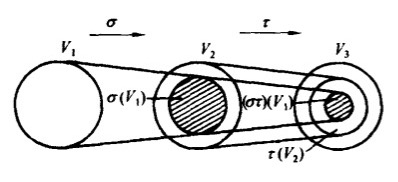
\includegraphics[scale=.5]{figs/5C.4.1.jpg}
          \end{figure}
          又因为 $ (\tau \sigma)(V_1) = \tau(\sigma(V_1)) $,所以又有
          \[ \dim(\tau \sigma)(V_1) \leqslant \dim \sigma(V_1) \]
          即 $ r(\tau \sigma) \leqslant r(\sigma) $.

          再证左边. 由线性映射维数公式,
          \begin{gather*}
              r(\tau) + \dim \ker \tau = n \\
              r(\tau \sigma) + \dim \ker(\tau \sigma) = m
          \end{gather*}
          又 $ \dim \ker(\tau \sigma) \leqslant \dim \ker \tau $,所以
          \[ m - r(\tau \sigma) = \dim \ker(\tau \sigma) \leqslant \dim \ker \tau \]
          代入线性映射维数公式,得 $ \dim \ker \tau = n - r(\tau) \geqslant m - r(\sigma) $,即
          \begin{align*}
              r(\tau \sigma) & \geqslant m + r(\tau) - n         \\
                             & \geqslant r(\sigma) + r(\tau) - n
          \end{align*}
        \end{answer}

        \item 设$V_1$是有限维线性空间,$\sigma,\tau\in \mathcal{L}(V_1,V_2)$,则
        \[r(\sigma+\tau) \leqslant r(\sigma)+r(\tau).\]

        事实上前两题的结论在后续章节矩阵的秩中都会涉及,此处有兴趣的同学可以尝试从线性映射的角度理解这两个秩不等式. 如果无法找到合适方式,可以考虑化为矩阵进行证明.
        \begin{answer}
            证明:由于 $ \forall \beta \in (\sigma + \tau)(V_1),\enspace \exists \alpha \in V_1 $ 使 $ \beta = (\sigma + \tau)(\alpha) = \sigma(\alpha) + \tau(\alpha) \in \sigma(V_1) + \tau(V_1) $,所以
          \[ (\sigma + \tau)(V_1) \subseteq \sigma(V_1) + \tau(V_1) \]
          因此
          \begin{align*}
              \dim(\sigma + \tau)(V_1) & \leqslant \dim(\sigma(V_1) + \tau(V_1))     \\
                                       & \leqslant \dim \sigma(V_1) + \dim \tau(V_1)
          \end{align*}
        \end{answer}
        \item 设$\sigma\in \mathcal{L}(V,V)$,$\dim V_1=n$,且$\sigma^2=\sigma$,$I$是$V$上的恒等变换. 证明:
        \begin{enumerate}
            \item $(I-\sigma)(V) \in \ker\sigma$;

            \item $r(I-\sigma)+r(\sigma)=n$.
        \end{enumerate}

        \begin{answer}
            \begin{enumerate}
                \item \label{item:5:C:6:1}
                      $ \forall \sigma \in \mathcal{L}(V, V) $,则 $ I - \sigma \in \mathcal{L}(V, V) $. $ \forall \alpha \in (I - \sigma)(V),\enspace \exists \beta \in V $,有
                      \begin{gather*}
                          \alpha = (I - \sigma)(\beta) = \beta - \sigma(\beta) \\
                          \sigma(\alpha) = \sigma(\beta - \sigma(\beta)) = \sigma(\beta) - \sigma^2(\beta)
                      \end{gather*}
                      而由于 $ \sigma^2 = \sigma $,所以 $ \sigma(\alpha) = \vec{0} $,于是 $ \alpha \in \ker \sigma $,因此 $ (I - \sigma)(V) \subseteq \ker \sigma $.

                \item 利用 $ r(\sigma + \tau) \leqslant r(\sigma) + r(\tau) $ 和 $ r(\sigma) + \dim \ker \sigma = n $,由 \ref*{item:6:C:4:1} 可得
                      \begin{equation} \label{eq:5:C:6:2:1}
                          r(I - \sigma) + r(\sigma) \leqslant n
                      \end{equation}
                      又因为
                      \begin{equation} \label{eq:5:C:6:2:2}
                          r(I - \sigma) + r(\sigma) \geqslant r(I - \sigma + \sigma) = r(I) = n
                      \end{equation}
                      于是由\autoref{eq:5:C:6:2:1} 和\autoref{eq:5:C:6:2:2} 即可得到 $ r(I - \sigma) + r(\sigma) = n $.
            \end{enumerate}
        \end{answer}


        \item 已知$V$为有限维线性空间,$\sigma\in \mathcal{L}(V,V)$,且$\sigma^2=\theta$(零映射). 证明:
        \begin{enumerate}
            \item $\sigma$的像空间维数不超过$\dfrac{n}{2}$;

            \item 设$A$是$\sigma$在某组基下的矩阵,则方程组$AX=0$的基础解系至少有$\dfrac{n}{2}$个解.
        \end{enumerate}
        \begin{answer}
            证明:\begin{enumerate}
                \item \label{item:5:C:7:1}
                      $ \forall \alpha \in \im \sigma,\enspace \exists \beta \in V $ 使得 $ \sigma(\beta) = \alpha $. 由 $ \sigma^2 = \theta $ 可得 $ \sigma(\alpha) = \sigma^2(\beta) = \vec{0} $,因此 $ \alpha \in \ker \sigma $,从而 $ \im \sigma \subseteq \ker \sigma $. 于是我们得到
                      \[ n = \dim \im \sigma + \dim \ker \sigma \geqslant 2 \dim \im \sigma \]
                      即 $ \dim \im \sigma \leqslant \dfrac{n}{2} $.

                \item 由 \ref*{item:5:C:7:1} 可知,方程组 $ AX = \vec{0} $ 的基础解系含有 $ n - r(A) = \dim \ker \sigma \geqslant \dfrac{n}{2} $ 个解向量,所以结论成立.
            \end{enumerate}

        \end{answer}
    \end{exgroup}
\end{exercise}

\chapter{线性映射矩阵表示}

在上一讲的讨论中我们定义了线性映射的基本概念与性质,以及线性映射像空间与核空间之间的关联,引出了我们目前为止最核心的概念——同构. 同构使得我们研究的抽象层次更上一层,而本讲将在这抽象的制高点获得最具象的表达形式——矩阵,介绍线性映射矩阵表示的定义,以及这一定义下线性映射与矩阵的一一对应关系,从而使得我们后续的研究都可以基于具象的矩阵.

\section{线性映射矩阵表示}

最开始我们在高斯消元时引入了矩阵作为符号简化和方程组求解的工具,严格地来说,我们之前的定义是:
\begin{definition}{}{}
    域$\mathbf{F}$中的$m\times n$个元素$a_{ij}\enspace(i=1,\ldots,m,\enspace j=1,\ldots,n)$排成$m$行$n$列的矩形数表,称为域$\mathbf{F}$上的一个$m\times n$矩阵,记作
    \[A=\begin{pmatrix}
            a_{11} & a_{12} & \cdots & a_{1n} \\
            a_{21} & a_{22} & \cdots & a_{2n} \\
            \vdots & \vdots & \ddots & \vdots \\
            a_{m1} & a_{m2} & \cdots & a_{mn}
        \end{pmatrix}\]
    或简记为$(a_{ij})_{m\times n}$,其中$a_{ij}$表示矩阵$A$的第$i$行第$j$列的元素.
\end{definition}

但是笔者将会在下文用不同的方式引出一种新的定义. 为了探究线性映射的性质,我们需要先研究一些特殊案例,然后从特殊到一般,矩阵就是对特殊案例——$\mathbf{F}^n$ 这样空间的研究. 不妨先考察 $\mathbf{F}^n\to\mathbf{F}^m$ 的线性映射,其可以写成 $y = \sigma(x)$,其中 $x\in\mathbf{F}^n, y\in\mathbf{F}^m$. 我们给出如下结论:
\begin{lemma}{}{}
    设
    \begin{align*}
        \sigma \colon \mathbf{F}^n &\to \mathbf{F}^m \\
        x = (x_1, \cdots, x_n) & \mapsto y = (y_1, \cdots, y_m)
    \end{align*}
    是线性映射,则映射具有形式,称矩阵 $(a_{ij})_{m\times n}$ 为线性映射 $\sigma\colon\mathbf{F}^n\to\mathbf{F}^m$ 的标准表示
    \begin{align*}
        y_1 &= a_{11} x_1 + a_{12} x_2 + \cdots + a_{1n} x_n \\
        y_2 &= a_{21} x_1 + a_{22} x_2 + \cdots + a_{2n} x_n \\
        & \cdots\\
        y_m &= a_{m1} x_1 + a_{m2} x_2 + \cdots + a_{mn} x_n
    \end{align*}
\end{lemma}
\begin{proof}
    考虑 $\sigma$ 在 $\mathbf{F}^n$ 的标准基底 $e_1, e_2, \ldots, e_n$ 上的值,设
    \[
        \sigma(e_1) = \begin{pmatrix} a_{11} \\ a_{21} \\ \vdots \\ a_{m1} \end{pmatrix},
        \sigma(e_2) = \begin{pmatrix} a_{12} \\ a_{22} \\ \vdots \\ a_{m2} \end{pmatrix},
        \ldots,
        \sigma(e_n) = \begin{pmatrix} a_{1n} \\ a_{2n} \\ \vdots \\ a_{mn} \end{pmatrix}
    \]
    由线性性,有
    \begin{align*}
        \sigma(x) &= \sigma(x_1 e_1 + x_2 e_2 + \cdots + x_n e_n) \\
        &= x_1 \sigma(e_1) + x_2 \sigma(e_2) + \cdots + x_n \sigma(e_n) \\
        &= \begin{pmatrix} a_{11} x_1 \\ a_{21} x_1 \\ \vdots \\ a_{m1} x_1 \end{pmatrix} +
        \begin{pmatrix} a_{12} x_2 \\ a_{22} x_2 \\ \vdots \\ a_{m2} x_2 \end{pmatrix} +
        \cdots +
        \begin{pmatrix} a_{1n} x_n \\ a_{2n} x_n \\ \vdots \\ a_{mn} x_n \end{pmatrix}\\
        &= \begin{pmatrix}
            a_{11} x_1 + a_{12} x_2 + \cdots + a_{1n} x_n \\
            a_{21} x_1 + a_{22} x_2 + \cdots + a_{2n} x_n \\
            \cdots\\
            a_{m1} x_1 + a_{m2} x_2 + \cdots + a_{mn} x_n
        \end{pmatrix}
    \end{align*}
\end{proof}

不难发现这里的 $a_{ij}$ 项实际上反映了输入的第 $j$ 项对输出的第 $i$ 项有多少权重,而只要确定了这 $m\times n$ 个权重,我们就得到了一个 $\mathbf{F}^n\to\mathbf{F}^m$ 的线性映射. 换言之,$\mathcal{L}(\mathbf{F}^n, \mathbf{F}^m)$ 和这些权重是一一对应的,于是一个映射可以等价地被记为一个矩阵,它接受一个 $\mathbf{F}^n$ 的向量,返回一个 $\mathbf{F}^m$ 的向量,由于标准基的存在,所以我们有自然同构 $\mathcal{L}(\mathbf{F}^n, \mathbf{F}^m) \cong \mathbf{F}^{m\times n}$ 后面不再区分 $\mathbf{F}^{m\times n}$ 和 $\mathcal{L}(\mathbf{F}^n, \mathbf{F}^m)$.
\[
    A = \begin{pmatrix}
        a_{11} & a_{12} & \cdots & a_{1n} \\
        a_{21} & a_{22} & \cdots & a_{2n} \\
        \vdots & \vdots & \ddots & \vdots \\
        a_{m1} & a_{m2} & \cdots & a_{mn}
    \end{pmatrix} \iff \forall x\in\mathbf{R}^n,
    A \begin{pmatrix}
        x_1 \\ x_2 \\ \vdots \\ x_n
    \end{pmatrix} = \begin{pmatrix}
        a_{11} x_1 + a_{12} x_2 + \cdots + a_{1n} x_n \\
        a_{21} x_1 + a_{22} x_2 + \cdots + a_{2n} x_n \\
        \cdots\\
        a_{m1} x_1 + a_{m2} x_2 + \cdots + a_{mn} x_n
    \end{pmatrix}
\]

我们可以这样计算矩阵作用在向量上的结果
\[
    \begin{pmatrix}
        1 & 2 & 3 \\ 4 & 5 & 6
    \end{pmatrix} \begin{pmatrix}
        7 \\ 8 \\ 9
    \end{pmatrix} = \begin{pmatrix}
        1\times 7 + 2\times 8 + 3\times 9 \\
        4 \times 7 + 5\times 8 + 6\times 9
    \end{pmatrix} = \begin{pmatrix}
        50 \\ 122
    \end{pmatrix}
\]

回顾第一章对线性方程的两种表示,一种是写成若干条方程,从行看去,每一行反映了输出的一项如何由输入线性组合得来. 另一种是像\autoref{线性方程的向量表示}中一样写成一条向量方程 $x_1\beta_1 + x_2\beta_2 + \cdots + x_n\beta_n = 0$,从列看去,每一列反映了输入的每一项会对输出产生怎么样的影响.

我们注意到虽然证明过程中我们假设了 $\sigma(e_j) = (a_{1j}, a_{2j}, \ldots, a_{mj})^{\mathrm{T}}$,但是即使把矩阵的列改成任意向量空间 $V$ 中的向量而非 $\mathbf{R}^m$ 中的向量也并不改变论证的有效性,也就是说矩阵的列完全可以被替换为任意向量空间中的元素,这样我们也就得到了 $\mathbf{R}^n \to V$ 的映射的一般表示方法——写成长度为 $n$ 的一行,每列分别是一个向量,例如当 $V = \mathbf{R}[x]_4$ 时,我们可以写出
\[
(1, x, x^2, x^3) \begin{pmatrix}
    1 \\ 2 \\ 3 \\ 4
\end{pmatrix} = 1 + 2x + 3x^2 + 4x^3
\]

我们可以将上面的运算称作使用 $\mathbf{F}^n$ 中向量的系数对一个向量组做线性组合. 特别地,由于基底也是一个向量组,当 $A$ 作为 $n$ 维向量空间 $V$ 的一个基底时,它作为 $\mathbf{F}^n\to V$ 的同构将坐标映射到空间中对应的点,和将点映射到坐标的坐标映射 $V\to\mathbf{F}^n$ 互为逆映射. 如果回顾\hyperlink{基底的矩阵写法}{基底的矩阵写法}我们便会发现前面的符号和此处达成了统一.

我们有一些常用的矩阵,例如零矩阵,即所有元素均为0的矩阵,通常记为$O$;单位矩阵也十分常见,它表示对角线上元素为1,其余元素为0的矩阵,通常记为$E$(若已知阶数为$n$也可特别记为$E_n$)其第 $j$ 列恰好为标准基底中的 $e_j$.

除此之外,我们通常记域$\mathbf{F}$上的$m\times n$矩阵全体为$\mathbf{F}^{m\times n}$或$\mathbf{M}_{m\times n}(\mathbf{F})$. 当$m=n$时矩阵称为方阵,域$\mathbf{F}$上全体$n$阶矩阵(或称$n$阶方阵)记为$\mathbf{F}^{n\times n}$或$\mathbf{M}_n(\mathbf{F})$.

在了解矩阵的定义之后,我们可以引入线性映射矩阵表示的概念. 经过前面大量的关于坐标同构的铺垫之后,想必读者对于如何将抽象的映射转化为矩阵有一个大致的思路,将一般的向量空间同构到我们熟悉的 $\mathbf{F}^n$,然后就可以得到矩阵表示. 但是在这之前笔者认为需要带读者了解交换图的基本工具

我们把空间抽象出来称为一个节点,空间之间的函数用箭头来表示,例如,如果有映射 $\psi\colon V_1 \to V_2, \sigma\colon V_2 \to V_3$,那么我们可以绘制交换图
\[
    \tikzcdset{arrow style=tikz, diagrams={>=stealth}}
    \begin{tikzcd}
        V_1 \arrow[r, "\psi"] & V_2 \arrow[r, "\sigma"] & V_3
    \end{tikzcd}
\]

交换图唯一的要求是从一个节点沿着箭头到另一个节点,函数的复合应当是相同的,例如在上面的图中,如果 $x\in V_1$ 经过两个映射,它会先变成 $\psi(x)$,然后得到 $\sigma(\psi(x)) = (\sigma\circ\psi)(x)$. 所以在上面的图中,如果要从 $V_1$ 引出一条箭头指向 $V_3$ 则这条箭头只能代表映射 $\sigma\circ\psi$(注意后经过的映射写在左侧,这与从左到右的书写习惯相反),类似地我们可以画出如下的图
\[
    \tikzcdset{arrow style=tikz, diagrams={>=stealth}}
    \begin{tikzcd}
        V_1 \arrow[r, "\psi"] \ar[rd, "\rho\circ\psi"'] & V_2 \arrow[d, "\rho"] \ar[rd, "\sigma\circ\rho"] \\ & V_3 \ar[r, "\sigma"'] & V_4
    \end{tikzcd}
\]

从图中我们可以读出 $\sigma\circ(\rho\circ\psi) = (\sigma\circ\rho)\circ\psi$,即映射复合的结合律. 自此,构造出指定的映射就可以图形化地表示成在图上画箭头,只要能够找到两个节点之间的一条通路,就能够通过映射的复合构造出一个映射.

接下来回到一般的线性映射. 我们知道一个 $\mathbf{F}$ 上的 $m\times n$ 矩阵可以作为一个 $\mathbf{F}^n\to\mathbf{R}^m$ 的映射,所以矩阵对应的应该是从 $\mathbf{F}^n$ 指向 $\mathbf{F}^m$ 的箭头. 一个向量组可以作为一个 $\mathbf{F}^n\to V$ 的映射,所以一个 $n$ 元向量组对应一条 $\mathbf{F}^n$ 指向 $V$ 的箭头. 对于基底这种特殊的向量组,其特性是可逆,于是在 $\mathbf{F}^n\to V$ 外可以另外添加一条反向的箭头表示坐标映射. 不妨设 $V_1$ 是 $\mathbf{F}$ 上的 $n$ 维向量空间,而 $V_2$ 是 $\mathbf{F}$ 上的 $m$ 维向量空间. 为了把映射 $\sigma\colon V_1\to V_2$ 用矩阵表示,我们需要先取两个基底:$B_1 = (\varepsilon_1, \varepsilon_2, \ldots, \varepsilon_n)\colon \mathbf{F}^n\to V_1$ 和 $B_2 = (\alpha_1, \alpha_2, \ldots, \alpha_m)\colon\mathbf{F}^m\to V_2$. 根据上面的两组基和一个映射画出交换图
\[
    \tikzcdset{arrow style=tikz, diagrams={>=stealth}}
    \begin{tikzcd}
        V_1 \arrow[r, "\sigma"]
        \arrow[d, gray, shift left, "B_1^{-1}"] &
        V_2 \arrow[d, gray, shift left, "B_2^{-1}"] \\
        \mathbf{F}^n \arrow[u, shift left, "B_1"] &
        \mathbf{F}^m \arrow[u, shift left, "B_2"]
    \end{tikzcd}
\]

这时构造出一个矩阵,即画出一条从 $\mathbf{F}^n\to\mathbf{F}^m$ 的箭头就十分自然了,只需要求出从 $\mathbf{F}^n$ 到 $\mathbf{F}^m$ 的映射复合就可以,沿着交换图的箭头不难读出我们所求的矩阵可以写成 $\mathbf{M}(\sigma) = B_2^{-1} \circ \sigma \circ B_1$. 又或者,如果考虑从 $\mathbf{F}^n$ 到 $V_2$ 的两条路径,也可以说它是唯一的矩阵使得 $\sigma \circ B_1 = B_2 \circ \mathbf{M}(\sigma)$
\[
    \tikzcdset{arrow style=tikz, diagrams={>=stealth}}
    \begin{tikzcd}
        V_1 \arrow[r, "\sigma"]
        \arrow[d, gray, shift left, "B_1^{-1}"] &
        V_2 \arrow[d, gray, shift left, "B_2^{-1}"] \\
        \mathbf{F}^n \arrow[u, shift left, "B_1"]
        \arrow[r, red, "\mathbf{M}(\sigma)"'] &
        \mathbf{F}^m \arrow[u, shift left, "B_2"]
    \end{tikzcd}
\]

事实上,如果从另一个角度思考,因为矩阵是多个$\mathbf{R}^m$中的向量并列在一起得到的方块,那么如何得到这些$\mathbf{R}^m$中的列向量呢?想必是某些向量在线性映射到达空间的一组基下的坐标. 于是我们很自然地可以接受下面的定义:
\begin{definition}{}{线性映射矩阵表示}
    设$B_1=\{\varepsilon_1,\varepsilon_2,\ldots,\varepsilon_n\}$是$V_1(\mathbf{F})$的基,$B_2=\{\alpha_1,\alpha_2,\ldots,\alpha_m\}$是$V_2(\mathbf{F})$的基. 则线性映射$\sigma \in \mathcal{L}(V_1,V_2)$被它作用于基$B_1$的像
    \[\sigma(B_1)=\{\sigma(\varepsilon_1),\sigma(\varepsilon_2),\ldots,\sigma(\varepsilon_n)\}\]
    所唯一确定,而$\sigma(B_1)$是$V_2$的子空间,于是其中元素都可以被基$B_2$线性表示,即
    \[ \begin{cases} \begin{aligned}
                \sigma(\varepsilon_1) & = a_{11}\alpha_1+a_{21}\alpha_2+\cdots+a_{m1}\alpha_m \\
                \sigma(\varepsilon_2) & = a_{12}\alpha_1+a_{22}\alpha_2+\cdots+a_{m2}\alpha_m \\
                                      & \vdotswithin{=}                                       \\
                \sigma(\varepsilon_n) & = a_{1n}\alpha_1+a_{2n}\alpha_2+\cdots+a_{mn}\alpha_m
            \end{aligned} \end{cases} \]
    将$\sigma(B_1)=\{\sigma(\varepsilon_1),\sigma(\varepsilon_2),\ldots,\sigma(\varepsilon_n)\}$关于基$B_2$的坐标排列成矩阵$\mathbf{M}(\sigma)$,即
    \[
        \mathbf{M}(\sigma)=\begin{pmatrix}
            a_{11} & a_{12} & \cdots & a_{1n} \\
            a_{21} & a_{22} & \cdots & a_{2n} \\
            \vdots & \vdots & \ddots & \vdots \\
            a_{m1} & a_{m2} & \cdots & a_{mn}
        \end{pmatrix}
    \]
    称$\mathbf{M}(\sigma)$为$\sigma$在基$B_1$和$B_2$下的矩阵表示,有时也称线性映射在基下的表示矩阵.
\end{definition}

如果分开来讨论映射 $\sigma \circ B_1 = B_2 \circ \mathbf{M}(\sigma) : \mathbf{F}^n\to V_2$ 中的每一列,线性映射矩阵 $\mathbf{M}(\sigma)$ 表示就是将线性映射 $\sigma$ 在一组基 $B_1$ 上的像在另一组基 $B_2$ 下的坐标表示按列排列得到的结果. 这一整体过程我们也可以用如下记号表示:
\begin{equation}\label{eq:7:线性映射矩阵表示}
    (\sigma(\varepsilon_1),\sigma(\varepsilon_2),\ldots,\sigma(\varepsilon_n))=(\alpha_1,\alpha_2,\ldots,\alpha_m)\mathbf{M}(\sigma).
\end{equation}

根据定义我们直接有如下简单的观察:
\begin{enumerate}
    \item 线性映射矩阵表示的结果是一个$m\times n$矩阵,其中$m$是到达空间的维数,$n$是出发空间的维数,特别注意此处有个次序的颠倒,务必区分清楚;

    \item 若$\sigma$在基下矩阵表示为$A=(a_{ij})_{m\times n}$,在出发空间的基的第$i$个向量在到达空间基下的坐标为$(a_{1i},a_{2i},\ldots,a_{mi})$,即矩阵$A$的第$i$列,或写为$\sigma(\varepsilon)=a_{1i}\alpha_1+a_{2i}\alpha_2+\cdots+a_{mi}\alpha_m$.
\end{enumerate}

想必有很多读者会心存疑惑:为什么我们要这么定义线性映射的矩阵表示呢?我们将在下一小节说明线性映射构成的线性空间与矩阵构成线性空间的同构时解释这一点. 现在先让我们完成以下几个例题熟悉定义:
\begin{example}{}{矩阵表示1}
    已知$\sigma \in \mathcal{L}(\mathbf{R}^3,\mathbf{R}^3)$且$\sigma(x_1,x_2,x_3)^{\color{lightgray}\mathrm{T}}=(x_1+x_2,x_1-x_3, x_2)^{\color{lightgray}\mathrm{T}}$
    \begin{enumerate}
        \item 求$\sigma$的像空间和核空间;

        \item 求$\sigma$关于$\mathbf{R}^3$自然基的矩阵.
    \end{enumerate}
\end{example}

\begin{solution}
    \begin{enumerate}
        \item 求像空间和核空间的方法我们在之前已经介绍过,我们为了计算方便取$\mathbf{R}^3$的自然基$e_1,e_2,e_3$计算有:
              \[
                \im\sigma
                =\spa(\sigma(e_1),\sigma(e_2),\sigma(e_3))
                =\spa(
                        (1,1,0)^{\color{lightgray}\mathrm{T}},
                        (1,0,1)^{\color{lightgray}\mathrm{T}},
                        (0,-1,0)^{\color{lightgray}\mathrm{T}}
                    )
                =\mathbf{R}^3
              \]
              对于核空间,解方程$\sigma(\alpha)=0$即可. 我们也可以用更简洁的方式书写:
              \[
                \ker\sigma
                =\{
                    (x_1,x_2,x_3)^{\color{lightgray}\mathrm{T}} \mid
                    \sigma(x_1,x_2,x_3)^{\color{lightgray}\mathrm{T}}
                    =(0,0,0)^{\color{lightgray}\mathrm{T}}
                \}
                =\{(0,0,0)^{\color{lightgray}\mathrm{T}}\}
              \]
              即方程只有零解,核空间可以记为$\ker\sigma=\{0\}$(只含零元的空间的一般记法).

        \item 我们根据\autoref{def:线性映射矩阵表示},应先写出$\sigma$在出发空间一组基(按题目要求是$\mathbf{R}^3$自然基)下的像,并将像表示为到达空间基(按题目要求是$\mathbf{R}^3$自然基)的线性组合,即
            \begin{gather*}
                \sigma(e_1) = (1,1,0)^{\color{lightgray}\mathrm{T}}
                =e_1+e_2=(e_1,e_2,e_3)\begin{pmatrix}
                    1 \\ 1 \\ 0
                \end{pmatrix} \\
                \sigma(e_2) = (1,0,1)^{\color{lightgray}\mathrm{T}}
                =e_1+e_3=(e_1,e_2,e_3)\begin{pmatrix}
                    1 \\ 0 \\ 1
                \end{pmatrix} \\
                \sigma(e_3) = (0,-1,0)^{\color{lightgray}\mathrm{T}}
                =-e_2=(e_1,e_2,e_3)\begin{pmatrix}
                    0 \\ -1 \\ 0
                \end{pmatrix}
            \end{gather*}
            接下来我们把坐标依次按列称矩阵就得到了本题需要求解的矩阵:
            \[
                \mathbf{M}(\sigma)=\begin{pmatrix}
                    1 & 1 & 0  \\
                    1 & 0 & -1 \\
                    0 & 1 & 0
                \end{pmatrix}
            \]
    \end{enumerate}
\end{solution}

有趣的是,在结合我个人的学习经历以及过往辅学的经验后,我总结出了第二问的一种常见的错误解法,这里我需要加粗强调,下面这种解法是\textbf{完全错误的!!!}这里展示这一解法是为了让读者将前面所学的知识完全厘清:

\begin{solution}[错误解法!!!]
    $
        \sigma(x_1,x_2,x_3)^{\color{lightgray}\mathrm{T}}
        =(x_1+x_2,x_1-x_3, x_2)=(x_1,x_2,x_3)\begin{pmatrix}
            1 & 1  & 0 \\
            1 & 0  & 1 \\
            0 & -1 & 0
        \end{pmatrix}
    $
\end{solution}

我们惊奇地发现,这一结果和我们前面得到的标准答案在向量的排列方式上发生了变化,即标准答案的1、2、3行变为了这里的1、2、3列,我们需要强调两点:
\begin{enumerate}
    \item 为什么这种解法是错误的:我们可以直接比较\autoref{eq:7:线性映射矩阵表示} 和这一解法中,\autoref*{eq:7:线性映射矩阵表示} 的等号左边是$n$个向量在$\sigma$下的像,而上述解法$\sigma(x_1,x_2,x_3)^{\color{lightgray}\mathrm{T}}$只是$\sigma$在一个向量下的像,这显然是不一样的!!!同样,等号右边括号内\autoref*{eq:7:线性映射矩阵表示} 是到达空间的一组基,而上述解法中仍然只是一个向量. 我们从未定义过这样解题的结果是什么,所以千万不能做这种无意义的事!!!

          容易导致混淆的原因可能在于我们书写$(x,y,z)$向量时是排列成一行的,可能看起来和$(e_1,e_2,e_3)$有点相似,但是如果我们回忆在第一章中的约定:写作行向量,实际是列向量,把 $\mathbf{R}^3$ 的向量按列书写之后我们得到的应该是
          \[
            \sigma\begin{pmatrix}
                x_1 \\ x_2 \\ x_3
            \end{pmatrix} = \begin{pmatrix}
                x_1 + x_2 \\ x_1 - x_3 \\ x_2
            \end{pmatrix} = \begin{pmatrix}
                1 & 1 & 0 \\ 1 & 0 & -1 \\  0 & 1 & 0
            \end{pmatrix} \begin{pmatrix}
                x_1 \\ x_2 \\ x_3
            \end{pmatrix} \implies
            \sigma = \begin{pmatrix}
                1 & 1 & 0 \\ 1 & 0 & -1 \\  0 & 1 & 0
            \end{pmatrix}
          \]
          当注意到这点之后,实际上我们也可以直接写出矩阵形式的 $\mathbf{R}^3 \to \mathbf{R}^3$ 的映射,由于标准基 $B_1 = B_2 = E$ 是单位阵,即恒同映射(坐标等于向量)所以 $\sigma\circ E = E\circ \mathbf{M}(\sigma)$ 退化为其标准表示 $\mathbf{M} = \sigma = \begin{pmatrix}
              1 & 1 & 0 \\ 1 & 0 & -1 \\  0 & 1 & 0
          \end{pmatrix}$.

    \item 为什么会出现行列互换这样的错误:
          事实上
          \[
            \sigma(x,y,z)^{\color{lightgray}\mathrm{T}}
            =\sigma(xe_1+ye_2+ze_3)
            =x\sigma(e_1)+y\sigma(e_2)+z\sigma(e_3)
            =(x,y,z)
            \begin{pmatrix}
                \sigma(e_1)^{\color{lightgray}\mathrm{T}} \\
                \sigma(e_2)^{\color{lightgray}\mathrm{T}} \\
                \sigma(e_3)^{\color{lightgray}\mathrm{T}}
            \end{pmatrix},
          \]
        这里将$\sigma(e_1),\sigma(e_2),\sigma(e_3)$的结果按行排列成矩阵,对比标准答案的 $(\sigma(e_1), \sigma(e_2), \sigma(e_3))$ 是将$\sigma(e_1),\sigma(e_2),\sigma(e_3)$在$\mathbf{R}^3$自然基下的坐标按列排列成矩阵,回忆$\mathbf{R}^n$向量在自然基下坐标是其本身这一性质,标准答案就是将$\sigma(e_1),\sigma(e_2),\sigma(e_3)$按列排列成矩阵,由此我们解释了行列互换发生的原因.
\end{enumerate}

这也就是为什么我强调读者不要参考之前提到的第二种方法\autoref{ex:线性映射的像空间求解2}来求解像空间——很容易导致这里矩阵表示犯这样的错误,并且容易导致初学时无法区分求解像空间和线性映射矩阵表示的方法. 在这里我必须再次强调:在没有完全熟练掌握这些概念和方法前,不要乱用方法!!!

接下来,我们还需要介绍旋转变换的矩阵表示
\begin{example}{}{}
    设$\sigma\colon\mathbf{R}^2\to\mathbf{R}^2$是绕原点逆时针旋转$\theta$角的变换,求$\sigma$在$\mathbf{R}^2$的自然基下的矩阵表示.
\end{example}
\begin{solution}
    求解的过程是很自然简单的,我们只需要考虑$\sigma$在常用基$e_1,e_2$下的像,即
    \[
    \begin{cases}
        \sigma(e_1)=\cos\theta e_1+\sin\theta e_2=(e_1,e_2)\begin{pmatrix}
            \cos\theta \\ \sin\theta
        \end{pmatrix} \\
        \sigma(e_2)=-\sin\theta e_1+\cos\theta e_2=(e_1,e_2)\begin{pmatrix}
            -\sin\theta \\ \cos\theta
        \end{pmatrix}
    \end{cases}
    \]
    故
    \[\mathbf{M}(\sigma)=\begin{pmatrix}
        \cos\theta & -\sin\theta \\
        \sin\theta & \cos\theta
    \end{pmatrix}\]

\end{solution}
这一矩阵形式可以记忆,在之后会多次出现.

\section{$\mathcal{L}(V_1,V_2)$与矩阵线性空间的同构}

本节我们将通过说明$\mathcal{L}(V_1,V_2)$与矩阵构成的线性空间的同构来解释为什么我们要这么定义线性映射的矩阵表示. 为了达到这一目标,我们首先需要证明这一同构.

\subsection{矩阵的加法和数乘}

回忆我们定义

本节我们将完善上一讲中同构的例子的细节,即若$\dim V_1(\mathbf{F})=m$,$\dim V_2(\mathbf{F})=n$,则 $\mathcal{L}(\mathbf{F}^n, \mathbf{F}^m)$ 中映射和其在 $\mathbf{F}^{m\times n}$ 中的标准表示一一对应. 于是 $\mathbf{F}^{m\times n}$ 便可以自然地从映射构成的线性空间 $\mathcal{L}(\mathbf{F}^n, \mathbf{F}^m)$ 中继承加法和数乘. 先考虑加法,由于 $(\sigma+\tau)(x) = \sigma(x) + \tau(x)$,令 $\sigma = (a_{ij})_{m\times n}, \tau = (b_{ij})_{m\times n}$ 则有
\begin{align*}
    &\phantom{=\ }((a_{ij})_{m\times n} + (b_{ij})_{m\times n})(x)\\
    &= (a_{ij})_{m\times n} (x) + (b_{ij})_{m\times n} (x) \\
    &= \begin{pmatrix}
        a_{11} x_1 + a_{12} x_2 + \cdots + a_{1n} x_n \\
        a_{21} x_1 + a_{22} x_2 + \cdots + a_{2n} x_n \\
        \cdots\\
        a_{m1} x_1 + a_{m2} x_2 + \cdots + a_{mn} x_n
    \end{pmatrix} + \begin{pmatrix}
        b_{11} x_1 + b_{12} x_2 + \cdots + b_{1n} x_n \\
        b_{21} x_1 + b_{22} x_2 + \cdots + b_{2n} x_n \\
        \cdots\\
        b_{m1} x_1 + b_{m2} x_2 + \cdots + b_{mn} x_n
    \end{pmatrix} \\
    &= \begin{pmatrix}
        (a_{11} + b_{11}) x_1 + (a_{12} + b_{12}) x_2 + \cdots + (a_{1n} + b_{1n}) x_n \\
        (a_{21} + b_{21}) x_1 + (a_{22} + b_{22}) x_2 + \cdots + (a_{2n} + b_{2n}) x_n \\
        \cdots\\
        (a_{m1} + b_{m1}) x_1 + (a_{m2} + b_{m2}) x_2 + \cdots + (a_{mn} + b_{mn}) x_n
    \end{pmatrix} \\
    &= \begin{pmatrix}
        a_{11} + b_{11} & a_{12} + b_{12} & \cdots & a_{1n} + b_{1n} \\
        a_{21} + b_{21} & a_{22} + b_{22} & \cdots & a_{2n} + b_{2n} \\
        \cdots\\
        a_{m1} + b_{m1} & a_{m2} + b_{m2} & \cdots & a_{mn} + b_{mn}
    \end{pmatrix}
    \begin{pmatrix}
        x_1 \\ x_2 \\ \vdots \\ x_n
    \end{pmatrix}
\end{align*}

即应该有
\[
    (a_{ij})_{m\times n} + (b_{ij})_{m\times n} = (a_{ij} + b_{ij})_{m\times n}
\]

类似地,由线性映射的数乘 $(\lambda \sigma)(x) = \lambda\cdot(\sigma(x)), \forall \lambda\in\mathbf{F}, x\in V$ 可以导出
\[
    \lambda (a_{ij})_{m\times n} = (\lambda a_{ij})_{m\times n} = \begin{pmatrix}
        \lambda a_{11} & \lambda a_{12} & \cdots & \lambda a_{1n} \\
        \lambda a_{21} & \lambda a_{22} & \cdots & \lambda a_{2n} \\
        \vdots & \vdots & \ddots & \vdots \\
        \lambda a_{m1} & \lambda a_{m2} & \cdots & \lambda a_{mn}
    \end{pmatrix}
\]

结合上面的推导,我们给出正式的矩阵加法和数乘定义
\begin{definition}{矩阵加法和数乘}{}
    (加法) 设 $A = (a_{ij})_{m\times n}, B = (b_{ij})_{m\times n} \in \mathbf{F}^{m\times n}$ 为矩阵,则定义
    \[
        A + B = \begin{pmatrix}
            a_{11} + b_{11} & a_{12} + b_{12} & \cdots & a_{1n} + b_{1n} \\
            a_{21} + b_{21} & a_{22} + b_{22} & \cdots & a_{2n} + b_{2n} \\
            \cdots\\
            a_{m1} + b_{m1} & a_{m2} + b_{m2} & \cdots & a_{mn} + b_{mn}
        \end{pmatrix}
    \]
    (数乘) 对 $\lambda\in\mathbf{F}$, 定义
    \[
        \lambda A = \begin{pmatrix}
            \lambda a_{11} & \lambda a_{12} & \cdots & \lambda a_{1n} \\
            \lambda a_{21} & \lambda a_{22} & \cdots & \lambda a_{2n} \\
            \vdots & \vdots & \ddots & \vdots \\
            \lambda a_{m1} & \lambda a_{m2} & \cdots & \lambda a_{mn}
        \end{pmatrix}
    \]
\end{definition}

前文已经证明了两个空间之间的全体线性映射构成线性空间,这里矩阵作为特殊的线性映射($\mathbf{F}^n\to\mathbf{F}^m$),自然关于继承来的加法和乘法构成线性空间.

% deprecated
% 为此我们需要理解矩阵的加法和数乘是怎么样的.
% 我们有一个非常自然的想法——既然 $V_1\to V_2$ 的全体线性映射关于线性映射加法和数乘构成线性空间,那么我们也许可以利用线性映射加法与数乘运算的矩阵表示来定义加法和数乘运算.

% 我们首先回顾线性映射的加法和数乘运算:设$\sigma,\tau\in \mathcal{L}(V_1,V_2)$,规定$\sigma$与$\tau$之和及$\lambda$与$\sigma$的数乘$\lambda\sigma$分别为
% \begin{gather*}
%     (\sigma+\tau)(\alpha)=\sigma(\alpha)+\tau(\alpha),\enspace\forall\alpha\in V_1 \\
%     (\lambda\sigma)(\alpha)=\lambda(\sigma(\alpha)),\enspace\forall\alpha\in V_1
% \end{gather*}

% 回顾线性映射的矩阵表示,我们实际上是要计算出线性映射在出发空间一组基下的像在到达空间一组基下的坐标然后按列排列. 我们取$V_1$的基$B_1=\{\varepsilon_1,\varepsilon_2,\ldots,\varepsilon_n\}$,$V_2$的基$B_2=\{\alpha_1,\alpha_2,\ldots,\alpha_m\}$,假设$\sigma$和$\tau$在$B_1$和$B_2$下的矩阵分别为$A=(a_{ij})_{m\times n}$和$B=(b_{ij})_{m\times n}$,则
% \begin{gather*}
%     \sigma(\varepsilon_i)=a_{1i}\alpha_1+a_{2i}\alpha_2+\cdots+a_{mi}\alpha_m \\
%     \tau(\varepsilon_i)=b_{1i}\alpha_1+b_{2i}\alpha_2+\cdots+b_{mi}\alpha_m.
% \end{gather*}
% 因此
% \[(\sigma+\tau)(\varepsilon_i)=(a_{1i}+b_{1i})\alpha_1+(a_{2i}+b_{2i})\alpha_2+\cdots+(a_{mi}+b_{mi})\alpha_m,\enspace i=1,2,\ldots,n\]
% 即$(\sigma+\tau)$矩阵表示$\mathbf{M}(\sigma+\tau)$的第$i$列元素为$A$和$B$的第$i$列对应元素相加. 由于$i$是任取的,因此$(\sigma+\tau)$的矩阵表示每一列都是$A$和$B$同一列对应元素相加,实际上对于整个矩阵而言就是矩阵相同位置元素相加,即
% \begin{align*}
%     \mathbf{M}(\sigma+\tau) & =\begin{pmatrix}
%                                    a_{11}+b_{11} & a_{12}+b_{12} & \cdots & a_{1n}+b_{1n} \\
%                                    a_{21}+b_{21} & a_{22}+b_{22} & \cdots & a_{2n}+b_{2n} \\
%                                    \vdots        & \vdots        & \ddots & \vdots        \\
%                                    a_{m1}+b_{m1} & a_{m2}+b_{m2} & \cdots & a_{mn}+b_{mn}
%                                \end{pmatrix}     \\
%                             & \triangleq\begin{pmatrix}
%                                             a_{11} & a_{12} & \cdots & a_{1n} \\
%                                             a_{21} & a_{22} & \cdots & a_{2n} \\
%                                             \vdots & \vdots & \ddots & \vdots \\
%                                             a_{m1} & a_{m2} & \cdots & a_{mn}
%                                         \end{pmatrix} + \begin{pmatrix}
%                                                             b_{11} & b_{12} & \cdots & b_{1n} \\
%                                                             b_{21} & b_{22} & \cdots & b_{2n} \\
%                                                             \vdots & \vdots & \ddots & \vdots \\
%                                                             b_{m1} & b_{m2} & \cdots & b_{mn}
%                                                         \end{pmatrix} \\
%                             & =\mathbf{M}(\sigma)+\mathbf{M}(\tau).
% \end{align*}
% 式中$\triangleq$表示定义,即定义矩阵加法为矩阵对应元素相加. 同理,我们也可以通过线性映射的数乘定义矩阵数乘运算如下:
% \[\mathbf{M}(\lambda\sigma)=\begin{pmatrix}
%         \lambda a_{11} & \lambda a_{12} & \cdots & \lambda a_{1n} \\
%         \lambda a_{21} & \lambda a_{22} & \cdots & \lambda a_{2n} \\
%         \vdots         & \vdots         & \ddots & \vdots         \\
%         \lambda a_{m1} & \lambda a_{m2} & \cdots & \lambda a_{mn}
%     \end{pmatrix}\triangleq\lambda\begin{pmatrix}
%         a_{11} & a_{12} & \cdots & a_{1n} \\
%         a_{21} & a_{22} & \cdots & a_{2n} \\
%         \vdots & \vdots & \ddots & \vdots \\
%         a_{m1} & a_{m2} & \cdots & a_{mn}
%     \end{pmatrix}=\lambda\mathbf{M}(\sigma).\]

事实上从运算的形式看,这非常符合我们对于矩阵加法和数乘的幻想,即矩阵加法就是对应元素相加,矩阵数乘就是对应元素乘以一个数.

此外,在利用线性映射的加法和数乘定义了非常自然的矩阵加法和数乘后,我们也可以直接通过加法和数乘的定义证明 $m\times n$ 矩阵全体关于这两种运算构成线性空间. 这里我们只需回顾线性空间运算的八条要求然后逐一验证即可,实际上非常简单,因此不在此赘述.

\subsection{同构的说明}

在上一小节中我们借助映射定义了矩阵的加法和数乘运算,也说明了全体$m\times n$矩阵关于这两种运算构成线性空间$\mathbf{F}^{m\times n}$,接下来我们需要讨论的是对于$n$维线性空间$V_1$和$m$维线性空间$V_2$,$\mathcal{L}(V_1,V_2)$与$\mathbf{F}^{m\times n}$的同构. 即我们需要定义一个线性双射$\sigma:\mathcal{L}(V_1,V_2)\to\mathbf{F}^{m\times n}$. 事实上我们只需要取一组基,然后利用线性映射矩阵表示,即定义
\[
    \tikzcdset{arrow style=tikz, diagrams={>=stealth}}
    \begin{tikzcd}
        V_1 \arrow[r, "\sigma"]
        \arrow[d, gray, shift left, "B_1^{-1}"] &
        V_2 \arrow[d, gray, shift left, "B_2^{-1}"] &
        \mathcal{L}(V_1, V_2) \arrow[d, thick, red, "\cong"]\\
        \mathbf{F}^n \arrow[u, shift left, "B_1"]
        \arrow[r, "\mathbf{M}(\sigma)"'] &
        \mathbf{F}^m \arrow[u, shift left, "B_2"] &
        \mathcal{L}(\mathbf{F}^n, \mathbf{F}^m) = \mathbf{F}^{m\times n}
    \end{tikzcd}
    \varphi(\sigma)=\mathbf{M}_{\color{lightgray} B_1, B_2}(\sigma)\\
\]

也就是说$\varphi$将线性映射$\sigma$映射为其矩阵表示. 接下来需要验证$\varphi$是线性双射.
\begin{enumerate}
    \item 先证明线性性,因为根据矩阵加法和数乘的定义和基、坐标的线性性,我们有
          \begin{align*}
            \forall x\in\mathbf{F}^n, \\
            (\varphi(\sigma + \tau))(x)
            &= (B_2^{-1} \circ (\sigma + \tau) \circ B_1) (x) \\
            &= B_2^{-1} ((\sigma + \tau) (B_1 (x))) \\
            &= B_2^{-1} (\sigma (B_1 (x)) + \sigma (B_1 (x))) \\
            &= B_2^{-1} (\sigma (B_1 (x))) + B_2^{-1} (\sigma (B_1 (x))) \\
            &= (B_2^{-1} \circ \sigma \circ B_1) (x) + (B_2^{-1} \circ \tau \circ B_1) (x) \\
            &= (\varphi(\sigma))(x) + (\varphi(\tau))(x) \\
            &= (\varphi(\sigma) + \varphi(\tau))(x)\\
            &\implies \varphi(\sigma + \tau) = \varphi(\sigma) + \varphi(\tau)\\
            (\varphi(\lambda\sigma))(x)
            &= (B_2^{-1} \circ (\lambda\sigma) \circ B_1)(x)\\
            &= B_2^{-1} ((\lambda\sigma)(B_1(x)))\\
            &= B_2^{-1} (\lambda (\sigma(B_1(x))))\\
            &= \lambda (B_2^{-1} (\sigma (B_1(x))))\\
            &= (\lambda (B_2^{-1}\circ\sigma\circ B_1))(x)\\
            &= (\lambda \varphi(\sigma))(x)\\
            &\implies \varphi(\lambda\sigma) = \lambda \varphi(\sigma)
          \end{align*}
          % deprecated
          %   \begin{gather*}
          %     \varphi(\sigma+\tau)(x)=\mathbf{M}(\sigma+\tau)=\mathbf{M}(\sigma)+\mathbf{M}(\tau)=\varphi(\sigma)+\varphi(\tau) \\
          %     \varphi(\lambda\sigma)=\mathbf{M}(\lambda\sigma)=\lambda\mathbf{M}(\sigma)=\lambda\varphi(\sigma).
          %   \end{gather*}

    \item 双射也是显然的:
          基底是可逆映射,故 $\varphi(\sigma) = B_2^{-1} \circ \sigma \circ B_1$ 和 $\varphi^{-1}(M) =  B_2 \circ M \circ B_1^{-1}$ 互为逆映射,从而是双射.
        %   \begin{enumerate}
        %     \item 对于单射性,我们考察$\varphi$的核空间$\ker\varphi$中的元素$\sigma$,即$\sigma$在基下的矩阵表示为零矩阵,那么$\sigma$必然为零映射,因为它将所有基映射为0,故必然将所有出发空间元素映射为0,因此核空间为$\{0\}$,单射成立;

        %     \item 对于满射性,我们需要为任意$m\times n$矩阵$(a_{ij})_{m\times n}$找到一个线性映射,使得这一矩阵为这一线性映射在基下的矩阵表示. 事实上,给定基和矩阵表示,我们就知道了线性映射在出发空间的基下的像——因为给定到达空间的基和矩阵就给定了线性映射在出发空间的基在到达空间的基下的坐标. 然后根据\autoref{thm:线性映射构造} 知我们一定能找到这一映射,故满射性成立.
        %   \end{enumerate}
\end{enumerate}

这一同构不仅体现在线性空间的同构,更是体现在作为映射保持了映射对象的同步运算,换言之,$X \mapsto \mathbf{M}(\sigma)(x)$ 和 $\alpha \mapsto \sigma(\alpha)$ 是同步进行的. 即我们有重要定理:

\begin{theorem}{线性映射对向量坐标的影响}{线性映射对向量坐标的影响}
    设$\sigma \in \mathcal{L}(V_1,V_2)$关于$V_1$和$V_2$的基$B_1$和基$B_2$的矩阵为$A=(a_{ij})_{m \times n}$,且$\alpha$与$\sigma(\alpha)$在基$B_1=(\alpha_1,\ldots,\alpha_n)$和$B_2=(\beta_1,\ldots,\beta_m)$下的坐标分别为$X$和$Y$,则$Y=AX$.
\end{theorem}

\begin{proof}
    设$X=(x_1,\ldots,x_n)^\mathrm{T},\enspace Y=(y_1,\ldots,y_m)^\mathrm{T}$,由题意可知
    \begin{align*}
        \sigma(\alpha) & =\sigma(x_1\alpha_1+\cdots+x_n\alpha_n)                                 \\
                       & =x_1\sigma(\alpha_1)+\cdots+x_n\sigma(\alpha_n)                         \\
                       & =(\sigma(\alpha_1),\ldots,\sigma(\alpha_n))X \\
                       & =(\beta_1,\ldots,\beta_m)AX
    \end{align*}
    又由于$\sigma(\alpha)$在线性无关向量组$\beta_1,\ldots,\beta_m$下的坐标唯一,故我们有$Y=AX$.
\end{proof}

或者通过画图来说明这一点,由于一个 $n$ 维的列向量可以认为属于 $\mathbf{F}^{n\times 1}$,即看成是 $\mathbf{F} \to \mathbf{F}^n$ 的矩阵(其乘以 $\mathbf{F}$ 中的标量 $k$ 等同于用 $k$ 数乘),假设向量 $\alpha, \sigma(\alpha)$ 在两个基底下分别有坐标 $X,Y$. 起手先画出我们熟悉的矩阵表示的图,然后向其上按照关系 $\alpha = B_1 X, \sigma(\alpha) = B_2 Y$ 添加箭头 $\alpha, X, Y$. 接下来就可以从图中直接读出 $Y=AX$
\[
    \tikzcdset{arrow style=tikz, diagrams={>=stealth}}
    \begin{tikzcd}
        V_1
            \arrow[r, "\sigma"]
            \arrow[d, gray, shift left, "B_1^{-1}"]
        & V_2
            \arrow[d, gray, shift left, "B_2^{-1}"]
        \\ \mathbf{F}^n
            \arrow[u, shift left, "B_1"]
            \arrow[r, "A"']
        & \mathbf{F}^m
            \arrow[u, shift left, "B_2"]
        \\ \color{red}\mathbf{F}
            \arrow[uu, red, bend left=60, "\alpha"]
            \arrow[u, red, "X"]
            \arrow[ur, red, "Y"']
    \end{tikzcd}
\]

解释如下:我们可以取任意的线性映射$\sigma:V_1\to V_2$,在$V_1$和$V_2$的基$B_1$和$B_2$下的矩阵表示为$A$. 这里有$V_1$和$V_2$中的向量在基下的坐标分别是$\mathbf{F}^n$和$\mathbf{F}^m$中的向量. 根据\autoref{thm:线性映射对向量坐标的影响},$\tau(\alpha)=\beta$中$\beta$和$\alpha$坐标之间的关联为$Y=AX$,这就相当于在$\mathbf{F}^n$和$\mathbf{F}^m$中的向量之间建立了一个与$A:V_1\to V_2$同步的映射$X\mapsto AX$,每当$V$中向量经过$\sigma$映射后,它的坐标也就经过了$A$的映射.

由此我们证明了$\mathcal{L}(V_1,V_2)\cong\mathbf{F}^{m\times n}$是一种线性映射层面的同构. 而我们很容易知道,$\mathbf{F}^{m\times n}$的维数为$mn$. 事实上对于矩阵关于矩阵加法和数乘构成的线性空间,我们有如下一组常用基:$E_{ij}(i=1,\ldots,m,j=1,\ldots,n)$,其中每个$E_{ij}$为第$i$行$j$列元素为1,其余元素全为0的矩阵. 例如对于$\mathbf{F}^{2\times 3}$,根据前面的描述我们可以写出其常用基为:
\[E_{11}=\begin{pmatrix}
        1 & 0 & 0 \\
        0 & 0 & 0
    \end{pmatrix},\enspace E_{12}=\begin{pmatrix}
        0 & 1 & 0 \\
        0 & 0 & 0
    \end{pmatrix},\enspace E_{13}=\begin{pmatrix}
        0 & 0 & 1 \\
        0 & 0 & 0
    \end{pmatrix},\]
\[E_{21}=\begin{pmatrix}
        0 & 0 & 0 \\
        1 & 0 & 0
    \end{pmatrix},\enspace E_{22}=\begin{pmatrix}
        0 & 0 & 0 \\
        0 & 1 & 0
    \end{pmatrix},\enspace E_{23}=\begin{pmatrix}
        0 & 0 & 0 \\
        0 & 0 & 1
    \end{pmatrix},\]
事实上,我们很容易验证这样的常用基的确是线性空间$\mathbf{F}^{m\times n}$的一组基,因为它们显然是线性无关的,且张成整个空间(请读者自行验证),然后我们也知道这样的常用基中矩阵有$m\times n$个,由此我们也得到了$\dim\mathcal{L}(V_1,V_2)=mn$. 当然我们还可以有另一种理解方式,如果读者已经学习过编程中二维数组的概念,事实上二维数组在计算机中的存储形式是一行存完接着马上存下一行,因此事实上我们可以将二维数组看作是一个长为$m\times n$的一维数组(方法就是第一行写完后在同一行马上接着写第二行元素,写完后在同一行接着写第三行元素,依此类推),因此我们也可以理解为$\mathbf{F}^{m\times n}$和$\mathbf{F}^{mn}$是没有区别的(容易验证是同构的),因此$\dim\mathbf{F}^{m\times n}=mn$.

\section{线性映射与矩阵的进一步讨论}

\begin{summary}

    在上一讲同构中我们已经知道,两个(有限维)线性空间中的元素是向量还是多项式还是函数并不是核心差别,只要它们维数相同,我们就可以遮蔽掉元素的差别——因为它们都可以通过坐标映射同构于 $\mathbf{F}^n$,因此一切线性空间在坐标作用下都变成了向量空间,变成了最直观的可以用一个一个数字写出来的向量,而本讲我们正基于此将所有无论多么抽象的线性映射也表示成能用一个一个数字写出来的东西,即所谓的矩阵. 我们利用坐标映射将之前抽象的线性空间和线性映射转化为具象的数字表达,使得我们之后的研究更加具体.

    在理解了线性映射矩阵表示的概念之后,我们给出了一个重要的例子,同时从反面给出了错误解法,希望读者务必厘清这其中涉及的各种概念和方法. 接下来我们证明了线性映射构成的线性空间与矩阵构成的线性空间同构,同时引入了矩阵的加法和数乘——这与线性映射的加法和数乘是完全对应的. 总而言之,在有了线性映射的矩阵表示后,我们便可以将抽象的研究都转化为具象的矩阵运算,这一思想我们将在介绍完需要的工具——矩阵运算以及行列式之后深入运用,届时我们将分别以抽象的线性映射理论和矩阵理论叙述大量的结论,探寻利用二者研究线性代数问题的过程的关联与差异.

\end{summary}

\begin{exercise}
    \exquote[S. 乌拉姆(Stanisław Ulam)]{一个定理有什么用并不重要,真正重要的是它有多优雅。}

    % \begin{exgroup}
    %
    % \end{exgroup}

    \begin{exgroup}[2] % 如果取消注释上面的 exgroup,删除此处 [2]
        \item 设$B=\{\beta_1,\beta_2,\ldots,\beta_n\}$是实数域$\mathbf{R}$上的线性空间$V$的一组基,$T \in L(V),\enspace T(\beta_1)=\beta_2,T(\beta_2)=\beta_3,\ldots,T(\beta_{n-1})=T(\beta_n),T(\beta_n)=\displaystyle\sum_{i=1}^{n}a_i\beta_i(a_i \in \mathbf{R})$,求$T$关于基$B$的表示矩阵,并求在什么条件下$T$是同构映射.

        \item 已知$f_1=1-x,f_2=1+x^2,f_3=x+2x^2$是$\mathbf{R}[x]_3$中三个元素,$\sigma$是$\mathbf{R}[x]_3$上的线性变换且满足$\sigma(f_1)=2+x^2,\sigma(f_2)=x,\sigma(f_3)=1+x+x^2$.
        \begin{enumerate}
            \item 证明:$f_1,f_2,f_3$构成$\mathbf{R}[x]_3$的一组基;

            \item 求$\sigma$在基$f_1,f_2,f_3$下的矩阵;

            \item 设$f=1+2x+3x^2$,求$\sigma(f)$.
        \end{enumerate}

        \item 设$V=\mathbf{M}_2(\mathbf{R})$是$\mathbf{R}$上所有$2 \times 2$矩阵构成的实数域上的线性空间. 已知
        \[A=\begin{pmatrix}1 & -1 \\ \lambda & 1 \end{pmatrix}(\lambda \in \mathbf{R}),\enspace B=\begin{pmatrix}1 & 2 \\ -1 & -1 \end{pmatrix}\]
        \begin{enumerate}
            \item 证明:$\varphi(X)=AXB$为$V$上的线性变换;

            \item 证明:$\lambda\neq-1$时,$\varphi$为可逆线性变换;

            \item \label{item:7:B:1}
                  $\lambda=-1$时,求$\varphi$的像空间和核空间;

            \item 将 \ref*{item:7:B:1} 中的值域扩充为$V$的一组基,并求$\varphi$在这组基下的矩阵.
        \end{enumerate}

        \item 设矩阵空间$\mathbf{R}^{2\times 2}$的子空间为
        \[V=\{X=(x_{ij})_{2\times 2} \mid x_{11}+x_{12}+x_{21}=0,\enspace x_{ij}\in \mathbf{R}\}\]
        V中的线性变换为$\sigma(X)=X+X^\mathrm{T}$,求$V$的一组基,使得$\sigma$在该基下的矩阵表示为对角矩阵.

        \item 设 $\mathbf{R}[x]_4$ 是数域 $\mathbf{R}$ 上次数小于 4 的多项式所构成的线性空间(约定零多项式次数为 $-\infty$). $\mathbf{M}_2(\mathbf{R})$ 是 $\mathbf{R}$ 上 2 阶方阵所构成的线性空间. 定义 $T \colon \mathbf{R}[x]_4 \to \mathbf{M}_2(\mathbf{R})$ 如下:对 $f(x) \in \mathbf{R}[x]_4$,
        \[T(f(x))=\begin{pmatrix}f(0) & f(1) \\ f(-1) & f(0)\end{pmatrix}\]
        \begin{enumerate}
            \item 求出 $T$ 的核空间 $N(T)$ 和像空间 $R(T)$;

            \item 求$T$在$\mathbf{R}[x]_4$和$\mathbf{M}_2(\mathbf{R})$的基下的矩阵表示.
        \end{enumerate}

        \item 设$A=\begin{pmatrix}
                1 & -1 & -1 \\ -1 & 1 & 1 \\ 0 & -4 & 2
            \end{pmatrix},\enspace\xi_1=(-1,1,-2)^\mathrm{T}$.
        \begin{enumerate}
            \item 求满足$A\xi_2=\xi_1$及$A^2\xi_3=\xi_1$的所有$\xi_2,\xi_3$;

            \item 证明:$\xi_1,\xi_2,\xi_3$线性无关.
        \end{enumerate}

        \item 已知$V$为有限维线性空间,$\sigma\in \mathcal{L}(V,V)$,且$\ker\sigma=\im \sigma$,证明:
        \begin{enumerate}
            \item $n$为偶数;

            \item 存在$V$的一组基$\alpha_1,\ldots,\alpha_n$使得
                  \[\sigma(\alpha_1,\ldots,\alpha_n)=(\alpha_1,\ldots,\alpha_n)\begin{pmatrix}
                          0 & E_{\frac{n}{2}} \\ 0 & 0
                      \end{pmatrix}.\]
        \end{enumerate}
    \end{exgroup}

    % \begin{exgroup}
    %
    % \end{exgroup}

\end{exercise}

\chapter{矩阵运算基础}

上一节我们将前面逐步搭建的线性空间与线性映射的抽象转变为具象的表达——矩阵——这是我们上一节最后内容总结中提到的利用坐标映射同构到最简单的向量空间的优越性的体现. 从本讲起的三讲内容中,我们的目光都会聚焦于具象的矩阵,但我们的视角时常会结合线性映射同步进行. 本讲我们首先介绍矩阵的基本运算的定义(及其与线性映射的关联)、性质与基本技巧,之后我们会在此基础上从线性映射的秩出发定义矩阵的秩,得到第一个重要的矩阵标准形——相抵标准形. 最后我们会更进一步加强运算技巧,介绍一些在解题或者是实际应用中常用的矩阵运算技巧.

\section{矩阵乘法}

\subsection{矩阵乘法的定义与基本性质}

我们在前文证明过线性映射的复合仍然是线性映射,当我们写出 $(\tau{\color{lightgray}\circ}\sigma)(\alpha) = \tau(\sigma(\alpha))$ 时我们通过映射复合定义了映射的乘法(只有这样才能在形式上说结合律成立). 于是矩阵作为一种特殊的映射,其乘法应当继承自矩阵的复合,我们注意到映射 $\tau\sigma$ 能够存在的条件是 $\tau$ 的出发空间和 $\sigma$ 的到达空间相同,即两个映射可以通过一个公共的中间空间``连接''起来
\[
    \tikzcdset{arrow style=tikz, diagrams={>=stealth}}
    \begin{tikzcd}
        V_1 \arrow[r, "\sigma"] \arrow[rr, bend right, "\tau{\color{lightgray}{}\circ{}}\sigma"'] & V_2 \arrow[r, "\tau"] & V_3
    \end{tikzcd}
\]

我们假设读者已经熟知映射的相乘即复合,在后文中我们将会省去映射复合的符号 ${\color{lightgray}\circ}$.  那么将 $V_1, V_2, V_3$ 分别替换为我们熟悉的 $\mathbf{F}^n, \mathbf{F}^m, \mathbf{F}^p$,我们就理应能够将 $p\times m$ 和 $m\times n$ 的两个矩阵相乘
\[
    \tikzcdset{arrow style=tikz, diagrams={>=stealth}}
    \begin{tikzcd}
        \mathbf{F}^n \arrow[r, "B"] \arrow[rr, bend right, "AB"'] & \mathbf{F}^m \arrow[r, "A"] & \mathbf{F}^p
    \end{tikzcd}
\]

由于复合的映射的复合是线性映射,那么矩阵的乘法应该给出一个矩阵 $AB\in\mathbf{F}^{p\times n}$. 那么让我们动手计算一下
\begin{align*}
    (AB)(x) &= A(Bx) \\
    &= \begin{pmatrix}
        a_{11} & a_{12} & \cdots & a_{1m} \\
        a_{21} & a_{22} & \cdots & a_{2m} \\
        \vdots & \vdots & \ddots & \vdots \\
        a_{p1} & a_{p2} & \cdots & a_{pm}
    \end{pmatrix} \left( \begin{pmatrix}
        b_{11} & b_{12} & \cdots & b_{1n} \\
        b_{21} & b_{22} & \cdots & b_{2n} \\
        \vdots & \vdots & \ddots & \vdots \\
        b_{m1} & b_{m2} & \cdots & b_{mn}
    \end{pmatrix} \begin{pmatrix}
        x_1 \\ x_2 \\ \cdots \\ x_n
    \end{pmatrix} \right)\\
    &= \begin{pmatrix}
        a_{11} & a_{12} & \cdots & a_{1m} \\
        a_{21} & a_{22} & \cdots & a_{2m} \\
        \vdots & \vdots & \ddots & \vdots \\
        a_{p1} & a_{p2} & \cdots & a_{pm}
    \end{pmatrix} \begin{pmatrix}
        \sum_{j=1}^n b_{1j} x_j \\
        \sum_{j=1}^n b_{2j} x_j \\
        \vdots \\
        \sum_{j=1}^n b_{mj} x_j
    \end{pmatrix} \\
    &= \begin{pmatrix}
        \sum_{k=1}^m a_{1k} b_{kj} x_j \\
        \sum_{k=1}^m a_{2k} b_{kj} x_j \\
        \vdots \\
        \sum_{k=1}^m a_{pk} b_{kj} x_j
    \end{pmatrix} \\
    &= \begin{pmatrix}
        \sum_{k=1}^m a_{1k} b_{k1} & \sum_{k=1}^m a_{1k} b_{k2} & \cdots & \sum_{k=1}^m a_{1k} b_{kn} \\
        \sum_{k=1}^m a_{2k} b_{k1} & \sum_{k=1}^m a_{2k} b_{k2} & \cdots & \sum_{k=1}^m a_{2k} b_{kn} \\
        \vdots & \vdots & \ddots & \vdots \\
        \sum_{k=1}^m a_{pk} b_{k1} & \sum_{k=1}^m a_{pk} b_{k1} & \cdots & \sum_{k=1}^m a_{pk} b_{kn}
    \end{pmatrix} \begin{pmatrix}
        x_1 \\ x_2 \\ \vdots \\ x_n
    \end{pmatrix}\\
\end{align*}

设 $C = AB$,则矩阵相乘结果中有
\[
    c_{ij} = \sum_{k=1}^m a_{ik} b_{kj}
\]

矩阵乘法 $AB$ 表现为 $A$ 的行和 $B$ 的列的点乘,于是我们可以给出矩阵乘法的定义:
\begin{definition}{}{}
    设$A=(a_{ij})_{p\times m},B=(b_{ij})_{m\times n}$,我们定义$A$与$B$的乘积矩阵$C=AB=(c_{ij})_{p\times n}$是一个$p\times n$矩阵,其中它的第$i$行第$j$列元素为矩阵$A$的第$i$行与矩阵$B$的第$j$列对应位置元素相乘后求和的结果,即
    \[
        c_{ij}
        =\sum_{k=1}^m a_{ik} b_{kj}
        =a_{i1}b_{1j}+a_{i2}b_{2j}+\cdots+a_{im}b_{mj}\enspace(i=1,\ldots,p,\enspace j=1,\ldots,n).
    \]
\end{definition}

这一定义带给我们的感受与我们在上一讲定义矩阵加法和数乘时的直观不同,如果脱离了映射复合的背景,在我们初看这一定义时必然会产生一个疑惑:为什么矩阵乘法定义得如此复杂,为什么不定义成两个矩阵对应元素相乘就可以了呢?事实上,只有这么定义,才能使结合律 $(AB)x = A(Bx)$ 在形式上变为可能,如果从输入第 $j$ 个分量对输出第 $i$ 个分量的权重来看,输入的第 $j$ 个分量可以通过 $b_{kj}, \enspace 1\leqslant k\leqslant m$ 对中间变量产生影响,而中间变量对输出第 $i$ 个分量的影响体现在 $a_{ik}, \enspace 1\leqslant k\leqslant m$,相乘时就必须要把这些影响对中间变量的每一项叠加起来,所以是 $a_{ik} b_{kj}$ 对 $k$ 的求和,最终导致了输入和输出指标固定,对中间指标求和. 如果从基的角度看:

\begin{enumerate}
    \item 设线性空间 $V_1(F), V_2(F), V_3(F)$ 的基分别为
    \begin{align*}
        B_1&=\{\varepsilon, \varepsilon_2,\ldots,\varepsilon_n\},
        B_2&=\{\zeta_1,\zeta_2,\ldots,\zeta_m\},
        B_3&=\{\eta_1,\eta_2,\ldots,\eta_p\}
    \end{align*}
    $\sigma \in L(V_1,V_2), \tau \in L(V_2,V_3)$,且 $\sigma, \tau$ 分别关于基 $B_1$ 和 $B_2$ 及基 $B_2$ 和 $B_3$ 的矩阵为 $B=(b_{i,j})_{m \times n}$ 和 $A=(a_{ij})_{p\times m}$,即:

          $M(\tau)=A=\begin{pmatrix}
                  a_{11} & a_{12} & \cdots & a_{1m} \\
                  a_{21} & a_{22} & \cdots & a_{2m} \\
                  \vdots & \vdots & \ddots & \vdots \\
                  a_{p1} & a_{p2} & \cdots & a_{pm}
              \end{pmatrix}$,
          $M(\sigma)=B=\begin{pmatrix}
                  b_{11} & b_{12} & \cdots & b_{1n} \\
                  b_{21} & b_{22} & \cdots & b_{2n} \\
                  \vdots & \vdots & \ddots & \vdots \\
                  b_{m1} & b_{m2} & \cdots & b_{mn}
              \end{pmatrix}$.

    \item 则 $\tau\sigma \in L(V_1,V_3)$ 关于基 $B_1$ 和 $B_3$ 的矩阵 $C=(c_{ij})_{p\times n}$ 中第 $j$ 列元素 $c_{1j},c_{2j},\ldots,c_{pj}$ 是 $\tau\sigma(\varepsilon_j)$ 在基 $B_3$ 下的坐标. 于是有:
          \begin{align*}
            \tau\sigma(\varepsilon_j)
            &=\tau(\sigma(\varepsilon_j))
            &=\tau\left(\sum_{k=1}^{m}b_{kj}\zeta_k\right) \\
            &=\sum_{k=1}^{m}b_{kj}\tau(\zeta_k) \\
            &=\sum_{k=1}^{m}b_{kj\left(\sum_{i=1}^{p}a_{ik}\eta_i\right) \\
            &=\sum_{i=1}^{p}\left(\sum_{k=1}^{m}a_{ik}b_{kj}\right)\eta_i
          \end{align*}

          即得:$c_{ij}=a_{i1}b_{1j}+a_{i2}b_{2j}+\cdots+a_{im}b_{mj}$. 换言之,表示矩阵的乘积等于乘积(复合)的表示矩阵,这也可以通过映射的复合得到简单的验证
          \begin{align*}
            \mathbf{M}_{\color{lightgray} B_2, B_3} (\tau) \mathbf{M}_{\color{lightgray} B_1, B_2} (\sigma)
            &= (B_3^{-1} \tau B_2) (B_2^{-1} \sigma B_1) \\
            &= B_3^{-1} \tau (B_2 B_2^{-1}) \sigma B_1 \\
            &= B_3^{-1} (\tau \sigma) B_1 \\
            &= \mathbf{M}_{\color{lightgray} B_1, B_3} (\tau \sigma)
          \end{align*}

          如果从交换图的视角看,我们可以通过绘制箭头简单地看出,根据映射复合构造出的三个表示矩阵显然满足 $\mathbf{M}_{\color{lightgray} B_2, B_3} (\tau) \mathbf{M}_{\color{lightgray} B_1, B_2} (\sigma) = \mathbf{M}_{\color{lightgray} B_1, B_3} (\tau \sigma)$:
          \[
            \tikzcdset{arrow style=tikz, diagrams={>=stealth}}
            \begin{tikzcd}
                V_1
                    \arrow[rr, "\sigma"]
                    \arrow[rrrr, bend left, "\tau\sigma"]
                    \arrow[d, shift left, lightgray, "B_1^{-1}"]
                && V_2
                    \arrow[rr, "\tau"]
                    \arrow[d, shift left, lightgray, "B_2^{-1}"]
                && V_3
                    \arrow[d, shift left, lightgray, "B_3^{-1}"]
                \\ \mathbf{F}^n
                    \arrow[u, shift left, "B_1"]
                    \arrow[rrrr, bend right, "\mathbf{M}_{\color{lightgray} B_1, B_3} (\tau\sigma)"']
                    \arrow[rr, "\mathbf{M}_{\color{lightgray} B_1, B_2} (\sigma)"']
                && \mathbf{F}^m
                    \arrow[u, shift left, "B_2"]
                    \arrow[rr, "\mathbf{M}_{\color{lightgray} B_2, B_3} (\tau)"']
                && \mathbf{F}^p
                    \arrow[u, shift left, "B_3"]
            \end{tikzcd}
          \]

          但是需要注意的是,这要求在两个映射矩阵表示的基底选择中,$V_2$ 选取的基底是相同的,否则这个过程就会失败,基底不同时我们就无法写出 $\mathbf{M}(\tau)\mathbf{M}(\sigma) = \mathbf{M}(\tau\sigma)$
          \[
            \tikzcdset{arrow style=tikz, diagrams={>=stealth}}
            \begin{tikzcd}
                & V_1
                    \arrow[rd, "\sigma"]
                    \arrow[rr, "\tau\sigma"]
                    \arrow[dl, shift left, lightgray, "B_1^{-1}"]
                && V_3
                    \arrow[dr, shift left, lightgray, "B_3^{-1}"]
                \\ \mathbf{F}^n
                    \arrow[ur, shift left, "B_1"]
                    \arrow[rrrr, bend right=90, "\mathbf{M}_{\color{lightgray} B_1, B_3} (\tau\sigma)"']
                    \arrow[rd, "\mathbf{M}_{\color{lightgray} B_1, B_2} (\sigma)"']
                && V_2
                    \arrow[ur, "\tau"]
                    \arrow[dl, shift left, lightgray, "B_2^{-1}"]
                    \arrow[dr, shift left, lightgray, "(B_2')^{-1}"]
                && \mathbf{F}^p
                    \arrow[ul, shift left, "B_3"]
                \\ & \mathbf{F}^m
                    \arrow[ur, shift left, "B_2"]
                    \arrow[rr, dashed, "?"']
                && \mathbf{F}^m
                    \arrow[ul, shift left, "B_2'"]
                    \arrow[ur, "\mathbf{M}_{\color{lightgray} B_2', B_3} (\tau)"']
            \end{tikzcd}
          \]
\end{enumerate}

接下来我们再给出两个线性映射的例子来理解矩阵乘法:
\begin{enumerate}
    \item 回顾上一节中提到的旋转$\theta$角的线性映射对应的矩阵$M_{\theta}=\begin{pmatrix}
                  \cos\theta & -\sin\theta \\
                  \sin\theta & \cos\theta
              \end{pmatrix}$. 我们考虑先旋转$\theta_1$,然后旋转$\theta_2$对应的两个变换$\sigma_1,\sigma_2$的复合$\sigma_2\sigma_1$,实际上就是旋转$\theta_1+\theta_2$角度,其矩阵表示为$M_{\theta_1+\theta_2}$,而矩阵乘法
          \begin{align*}
              M_{\theta_2}M_{\theta_1}
               & =\begin{pmatrix}
                      \cos\theta_2 & -\sin\theta_2 \\
                      \sin\theta_2 & \cos\theta_2
                  \end{pmatrix}\begin{pmatrix}
                                   \cos\theta_1 & -\sin\theta_1 \\
                                   \sin\theta_1 & \cos\theta_1
                               \end{pmatrix} \\
               & =\begin{pmatrix}
                      \cos\theta_2\cos\theta_1-\sin\theta_2\sin\theta_1 & -\cos\theta_2\sin\theta_1-\sin\theta_2\cos\theta_1 \\
                      \sin\theta_2\cos\theta_1+\cos\theta_2\sin\theta_1 & -\sin\theta_2\sin\theta_1+\cos\theta_2\cos\theta_1
                  \end{pmatrix} \\
               & =\begin{pmatrix}
                      \cos(\theta_1+\theta_2) & -\sin(\theta_1+\theta_2) \\
                      \sin(\theta_1+\theta_2) & \cos(\theta_1+\theta_2)
                  \end{pmatrix}=M_{\theta_1+\theta_2},
          \end{align*}
          这表明矩阵乘法$M_{\theta_2}M_{\theta_1}$的结果确实与$\sigma_2\sigma_1$的矩阵表示$M_{\theta_1+\theta_2}$一致.

    \item 我们在此再次强调矩阵相乘时左侧矩阵的列数应该等于右边矩阵的行数:回顾线性映射的复合,若复合$\sigma_1\sigma_2$符合定义,则必须有$\sigma_2$的到达空间恰好是$\sigma_1$的出发空间,故两空间维数一致,那么$\sigma_1$对应的矩阵$A$的列数和$\sigma_2$对应的矩阵$B$的行数一致,这也是我们要求两个矩阵$A,B$可乘的重要条件的来源. 而最后乘法的结果行数等于$A$的行数,列数等于$B$的列数,这也与$\sigma_1\sigma_2$出发空间为$\sigma_2$出发空间(对应于$B$的列数),到达空间为$\sigma_1$到达空间(对应于$A$的行数)一致.
\end{enumerate}

\begin{example}{}{}
    设$A=\begin{pmatrix}
            1 & 0 & -1 \\
            1 & 1 & -3
        \end{pmatrix}, B=\begin{pmatrix}
            0 & 3 \\
            1 & 2 \\
            3 & 1
        \end{pmatrix}$,求$AB$和$BA$.
\end{example}

\begin{solution}
    $AB =\begin{pmatrix}
            0-3 & 3-1   \\
            1-9 & 3+2-3
        \end{pmatrix}=\begin{pmatrix}
            -3 & 2 & -8 & 2
        \end{pmatrix}$,

    $BA=\begin{pmatrix}
            0+3 & 0+3 & 0-9  \\
            1+2 & 0+2 & -1-6 \\
            3+1 & 0+1 & -3-3
        \end{pmatrix}=\begin{pmatrix}
            3 & 3 & -9 \\
            3 & 2 & -7 \\
            4 & 1 & -6
        \end{pmatrix}$.
\end{solution}

接下来给出矩阵运算的几个基本性质:
\begin{enumerate}
    \item $(AB)C=A(BC)$(结合律)

    \item $\lambda(AB)=(\lambda A)B=A(\lambda B),\enspace \lambda \in \mathbf{F}$

    \item $A(B+C)=AB+AC$(左分配律)

    \item $(B+C)P=BP+CP$(右分配律)
\end{enumerate}
证明方法十分简单:使用映射的结合律、线性性和分配律直接证明几何,或者直接暴力设出矩阵元素然后暴力计算证明等号两边对应位置(如第$i$行第$j$列元素)相等也是可行的.

实际上,由矩阵加法和乘法满足的运算律可知,全体$n$阶方阵构成的集合$\mathbf{F}^{n\times n}$关于矩阵加法和乘法构成环.

在本节最后,我们有四个非常重要的问题需要仔细探讨:
\begin{enumerate}
    \item 在有了矩阵乘法的定义后,高斯消元法中我们将线性方程组简记为$AX=b$实际上是相当自然的,除此之外,我们将向量坐标表示为列向量的形式,例如将向量 $v$ 对基 $\alpha$ 分解
          \[v=(\alpha_1,\alpha_2,\ldots,\alpha_n)\begin{pmatrix}
                  x_1 \\ x_2 \\ \vdots \\ x_n
              \end{pmatrix}\]
          这也是符合矩阵形式乘法定义的一种习惯(虽然基一般不是数域$\mathbf{F}$或者向量空间$\mathbf{F}^m$中的元素).

    \item 事实上,在这里我们可以看出求解线性方程组和线性映射之间的关联. 我们设$AX=b$的解为
          \[X=\begin{pmatrix}
                  x_1 \\ x_2 \\ \vdots \\ x_n
              \end{pmatrix}\]
          由$AX=b$和线性映射矩阵表示,我们有
          \begin{equation}\label{eq:7:方程组与核空间1}
              (\sigma(\varepsilon_1),\sigma(\varepsilon_2),\ldots,\sigma(\varepsilon_n))\begin{pmatrix}
                  x_1 \\ x_2 \\ \vdots \\ x_n
              \end{pmatrix}=(\alpha_1,\alpha_2,\ldots,\alpha_m)A\begin{pmatrix}
                  x_1 \\ x_2 \\ \vdots \\ x_n
              \end{pmatrix}=b
          \end{equation}
          即$x_1\sigma(\varepsilon_1)+x_2\sigma(\varepsilon_2)+\cdots+x_n\sigma(\varepsilon_n)=b$,即
          \begin{equation}\label{eq:7:方程组与核空间2}
              \sigma(x_1\varepsilon_1+x_2\varepsilon_2+\cdots+x_n\varepsilon_n)=b.
          \end{equation}
          由此我们将线性方程组的求解问题和找到线性映射到达空间中某个向量在出发空间中原像的坐标联系起来了,即将求解$AX=b$和求解$\sigma(a)=b$联系起来了,只是我们求解后者时通常是对于一般的向量空间而言的,这时求解是通过求出$a$在矩阵表示基下的坐标实现的.

          若前述$b=0$,则我们将齐次线性方程组的解空间与线性映射的核空间联系起来了,即线性映射的核空间中元素在一组基下的向量就是这一线性映射在这组基下的矩阵表示作为系数矩阵的线性方程组的解. 这一联系将在\nameref{chap:朝花夕拾}中有更深入的讨论.

    \item 我们可以更进一步理解矩阵乘法. 假设矩阵$A=(a_{ij})_{m\times n}$与$B=(b_{ij})_{n\times l}$相乘,我们有如下结论:
          \begin{enumerate}
              \item 乘积的第$k$列等于$A$乘以$B$的第$k$列,乘积的第$j$行等于$A$的第$j$行乘以$B$,这一点根据矩阵乘法计算方式显然,我们可以利用这一性质证明下面例子的结论:
                    \begin{example}{}{}
                        设$A,B$都是由非负实数组成的矩阵且$AB$有一行等于0,证明:或者$A$有一行为0,或者$B$有一行为0.
                    \end{example}
                    \begin{proof}
                        设$A=(a_{ij})_{m\times n}$,$B=(b_{ij})_{n\times l}$,且设$AB=(c_{ij})_{m\times l}$的第$i$行为0,则根据前面的讨论可知就是$A$的第$i$行乘以$B$得到了全0行向量. 因此若$A$的第$i$行为0,则结论成立;否则$A$的第$i$行中存在某个元素大于0,不妨设$a_{ik}>0$,则此时$B$的第$k$行各元素必须均为0,否则若$b_{kj}>0$,我们有
                        \[c_{ij}=a_{i1}b_{1j}+\cdots+a_{ik}b_{kj}+\cdots+a_{in}b_{nj}>0,\]
                        综上可知结论成立.
                    \end{proof}

              \item 乘积的每一列都是矩阵$A$各列的线性组合,每一行都是矩阵$B$各行的线性组合. 我们简要说明前者,后者理由类似. 我们考察乘积的每一列,由1可知乘积的第$k$列等于$A$乘以$B$的第$k$列,我们展开写乘积矩阵$C=(c_{ij})_{m\times l}$第$k$列的结果:
                    \begin{align*}
                        c_{1k} & =a_{11}b_{1k}+a_{12}b_{2k}+\cdots+a_{1n}b_{nk} \\
                        c_{2k} & =a_{21}b_{1k}+a_{22}b_{2k}+\cdots+a_{2n}b_{nk} \\
                               & \vdotswithin{=}                                \\
                        c_{mk} & =a_{m1}b_{1k}+a_{m2}b_{2k}+\cdots+a_{mn}b_{nk}
                    \end{align*}
                    我们将上面的行进行组合,写成列向量形式,即
                    \[\begin{pmatrix}
                            c_{1k} \\ c_{2k} \\ \vdots \\ c_{mk}
                        \end{pmatrix}=b_{1k}\begin{pmatrix}
                            a_{11} \\ a_{21} \\ \vdots \\ a_{m1}
                        \end{pmatrix}+b_{2k}\begin{pmatrix}
                            a_{12} \\ a_{22} \\ \vdots \\ a_{m2}
                        \end{pmatrix}+\cdots+b_{nk}\begin{pmatrix}
                            a_{1n} \\ a_{2n} \\ \vdots \\ a_{mn}
                        \end{pmatrix}\]
                    由此我们将乘积的列表示成了矩阵$A$各列的线性组合.
          \end{enumerate}

    \item 之后我们会经常看见两种记号,即
          \begin{align*}
              (\sigma(\varepsilon_1),\sigma(\varepsilon_2),\ldots,\sigma(\varepsilon_n))
              & =(\alpha_1,\alpha_2,\ldots,\alpha_m)A \\
              \sigma(\varepsilon_1,\varepsilon_2,\ldots,\varepsilon_n)
              & =(\alpha_1,\alpha_2,\ldots,\alpha_m)A
          \end{align*}
          教材中两个记号是等价的,这只是记号上的差别,含义完全相同. 但是在之后我们还会看到一个很特别的书写方式
          \[
            (\sigma(\varepsilon_1,\varepsilon_2,\ldots,\varepsilon_n))B
            =\sigma((\varepsilon_1,\varepsilon_2,\ldots,\varepsilon_n)B)
          \]
          教材不加解释地使用了这一等式,这容易导致读者的困惑,因此我们这里简要说明它们的确是等价的,从而接下来读者可以放心地自由使用这一结论.

          根据上述的第一个性质可知,我们只需要证明对$B$的某一列上式成立即可,因为乘法结果是列与列对应的. 我们设$B$的第$k$列为
          \[B_k=\begin{pmatrix}
                  b_{1k} \\ b_{2k} \\ \vdots \\ b_{nk}
              \end{pmatrix}\]
          则
          \begin{align*}
              (\sigma(\varepsilon_1,\varepsilon_2,\ldots,\varepsilon_n))
              \begin{pmatrix}
                  b_{1k} \\ b_{2k} \\ \vdots \\ b_{nk}
              \end{pmatrix}
               & =(\sigma(\varepsilon_1),\sigma(\varepsilon_2),\ldots,\sigma(\varepsilon_n))\begin{pmatrix}
                                                                                                b_{1k} \\ b_{2k} \\ \vdots \\ b_{nk}
                                                                                            \end{pmatrix} \\
               & =b_{1k}\sigma(\varepsilon_1)+b_{2k}\sigma(\varepsilon_2)+\cdots+b_{nk}\sigma(\varepsilon_n)                    \\
               & =\sigma(b_{1k}\varepsilon_1+b_{2k}\varepsilon_2+\cdots+b_{nk}\varepsilon_n)                                    \\
               & =\sigma((\varepsilon_1,\varepsilon_2,\ldots,\varepsilon_n)
              \begin{pmatrix}
                  b_{1k} \\ b_{2k} \\ \vdots \\ b_{nk}
              \end{pmatrix})
          \end{align*}
          故得证.
\end{enumerate}

事实上矩阵乘法有很多和数的乘法重要的不同,我们在此特别指出供读者参考:
\begin{enumerate}[label=(\arabic*)]
    \item 矩阵乘法不一定满足交换律(即$AB$不一定等于$BA$,事实上随手写两个矩阵,很大的概率就是不交换的,甚至交换过来不可乘). 因此实数的完全平方公式代入矩阵不一定成立,即很多时候$(A+B)^2=A^2+AB+BA+B^2\neq A^2+2AB+B^2$;

    \item 但是注意数量矩阵(即对角线上元素都相等,其余均为0,单位矩阵是其特例)和任何同阶的矩阵相乘都是可交换的,这一点在矩阵求幂时很有用;

    \item \label{item:7:矩阵乘法:3}
          $A\neq O$且$B\neq O$不能推出$AB\neq O$. 例如线性方程组$AX = 0$有非零解,若$B$的各列均为方程非零解,则$AB = O$ 在环上这种元素通常被称为零因子.

    \item 消去律也不一定满足:即$AB = AC$不一定$A = B$. 原因在于$AB=AC \implies A(B-C)=O$,由 \ref*{item:7:矩阵乘法:3} 可知不一定$B = C$.
\end{enumerate}

\subsection{矩阵多项式}

我们在线性空间中已经介绍过,我们一般用$\mathbf{F}[x]_{m+1}$表示数域$\mathbf{F}$上的次数最高为$m$的多项式全体,其中的元素我们一般记为
\[p(x)=a_mx^m+a_{m-1}x^{m-1}+\cdots+a_1x+a_0,\enspace a_i\in\mathbf{F}\enspace(i=1,2,\ldots,m)\]
我们发现这里的自变量不一定需要是一个数,也可以是线性变换或者方阵,因为只要可以和自己相乘就能定义乘方. 例如线性映射$\sigma:V\to V$构成的$m$次多项式可以记为
\[p(\sigma)=a_m\sigma^m+a_{m-1}\sigma^{m-1}+\cdots+a_1\sigma+a_0I\]
其中$\sigma^i$表示$\sigma$复合$i$次,$I$表示恒等映射. 我们很容易说明当$\sigma$在$V$的一组基下矩阵表示为$A$时,$p(\sigma)$在同一组基下的矩阵表示为
\[p(A)=a_mA^m+a_{m-1}A^{m-1}+\cdots+a_1A+a_0E,\]
其中$E$表示单位矩阵. 由此我们便得到了矩阵多项式的定义,我们有如下几点需要强调:
\begin{enumerate}
    \item 这里我们要求$\sigma$是线性变换(即出发空间和到达空间一致),因为只有满足这一条件才能复合. 对于矩阵而言,其作用在标准 $n$ 维向量空间 $\mathbf{F}^n$ 上,所以矩阵可求幂即要求出发空间和到达空间维数相同即可,这样才能保证矩阵的幂次可以定义(即$A$和$A$可乘,因此$A$的行列数一致);

    \item 上面的定义隐含:$\sigma^0 = I, A^0=E$;

    \item $A^kA^m=A^{k+m},\enspace (A^k)^m=A^{km}$,其中$A$为方阵,$k,m$为任意正整数. 当 $A$ 可逆时这一式可以拓展到全体整数,负整数对应于逆矩阵的情况,接下来可逆的部分会作进一步解释.
\end{enumerate}

\begin{example}{}{}
    展开矩阵多项式$(A+\lambda E)^n$.
\end{example}

\begin{solution}
    由于$A$与$E$是可交换的,并且$A^nE^m=A^n$显然成立,因此我们结合中学学过的二项式展开,得到结果:
    \begin{align*}
        (A+\lambda E)^n & =\sum_{i=0}^nC_n^iA^i(\lambda E)^{n-i}    \\
                        & =\sum_{i=0}^nC_n^i\lambda^{n-i}A^iE^{n-i} \\
                        & =\sum_{i=0}^nC_n^i\lambda^{n-i}A^i.
    \end{align*}
\end{solution}

\begin{example}{}{矩阵多项式可交换}
    设$f(x),g(x) \in \mathbf{F}[x],\enspace A,B \in \mathbf{M}_n(\mathbf{F})$. 证明:
    \begin{enumerate}
        \item $f(A)g(A)=g(A)f(A)$;

        \item 如果$AB=BA$,则$f(A)g(B)=g(B)f(A)$;
    \end{enumerate}
\end{example}

\begin{solution}
    我们可以直接证明第二点,因为第一点是第二点的特例. 设$f(x)=\displaystyle\sum_{i=0}^ma_ix^i$,$g(x)=\displaystyle\sum_{j=0}^sb_jx^j$,$A^0=B^0=E$,则
    \begin{align*}
        f(A)g(B) & =\sum_{i=0}^ma_iA^i\cdot \sum_{j=0}^sb_jB^j\quad(AB=BA)                            \\
                 & =\sum_{k=0}^{m+s}\sum_{i+j=k}a_ib_jA^iB^j=\sum_{k=0}^{m+s}\sum_{i+j=k}b_ja_iB^jA^i \\
                 & =g(B)f(A).
    \end{align*}
    事实上由于$A\cdot A=A\cdot A$,因此$f(A)g(A)=g(A)f(A)$只是上面证明的结论的特例.
\end{solution}

\section{一组例题}

在介绍了矩阵乘法后,我们可以进一步审视线性映射矩阵表示的定义. 我们来看一组初学时可能混淆或者不理解的例子,从而加深对概念的理解:
\begin{example}{}{矩阵表示2}
    设$A=\begin{pmatrix}1 & 0 & 2 \\ -1 & 2 & 1 \\ 1 & 2 & 5\end{pmatrix}$为两个三维线性空间之间的线性映射$\sigma$对应的矩阵,求$\sigma$的像空间和核空间.
\end{example}
(注:本题没有给出线性映射出发空间和到达空间的基,读者可以任意假设.)

\begin{solution}
    求解像空间和核空间,仍然是原先介绍的方法,虽然本题没有给出线性映射的直接定义,但矩阵表示也能给我们足够的信息. 我们设这一矩阵表示的线性映射为$\sigma$,且
    \[(\sigma(\varepsilon_1),\sigma(\varepsilon_2),\sigma(\varepsilon_3))=(\alpha_1,\alpha_2,\alpha_3)A\]
    根据线性映射矩阵表示的定义,我们知道矩阵表示就是线性映射在出发空间一组基下的像在到达空间一组基下的坐标按列排列,因此
    \begin{align*}
        \sigma(\varepsilon_1) & =\alpha_1-\alpha_2+\alpha_3   \\
        \sigma(\varepsilon_2) & =2\alpha_2+2\alpha_3          \\
        \sigma(\varepsilon_3) & =2\alpha_1+\alpha_2+5\alpha_3
    \end{align*}
    因此$\im\sigma=\spa(\alpha_1-\alpha_2+\alpha_3,2\alpha_2+2\alpha_3,2\alpha_1+\alpha_2+5\alpha_3)$,然后求解极大线性无关组即可,结果为$\im\sigma=\spa(\alpha_1-\alpha_2+\alpha_3,2\alpha_2+2\alpha_3)$

    这里求解极大线性无关组的方法我们可以回忆\autoref{ex:转化为坐标},我们先将三个向量转化为到达空间基下坐标,然后求解极大线性无关组,最后把基添加回来即可. 实际上我们会发现,这里的三个坐标就是矩阵$A$的三个列向量(因为矩阵表示就是线性映射在出发空间一组基下的像在到达空间一组基下的坐标按列排列),因此我们只需要求解矩阵$A$的列向量的极大线性无关组$(1,-1,1),(0,2,2)$,然后再将到达空间的基添加回来即可.

    然后求解核空间,我们设$\sigma(\varepsilon)=0$,将$\varepsilon$写成出发空间基的表示后事实上就是\autoref{eq:7:方程组与核空间2} 的形式,我们已说明这一形式与\autoref{eq:7:方程组与核空间1} 等价,因此我们只需求解$AX=0$然后代回出发空间的基即可,最终结果为$\ker\sigma=\spa(4\varepsilon_1+3\varepsilon_2-2\varepsilon_3)$.
\end{solution}

总结一下,此类题目求解像空间实际上就是求出矩阵列向量的极大线性无关组,然后记得将结果对到达空间的基向量做线性组合. 求解核空间只需求解齐次线性方程组$AX=0$并将解对出发空间的基向量即可.

\begin{example}{}{矩阵表示3}
    已知3阶矩阵$A=\begin{pmatrix}
            1 & 0 & 1 \\ 0 & -1 & 0 \\ -1 & 1 & -1
        \end{pmatrix}$. 定义$\mathbf{R}^{3 \times 3}$上的线性变换$\sigma(X)=AX,\enspace X \in \mathbf{R}^{3 \times 3}$. 求$\sigma$的像和核.
\end{example}

\begin{solution}
    核空间求解较为简单,我们先求解核空间. 我们首先求解线性方程组$AY=0$,其中$Y$为列向量,解得其基础解系为$\eta=(1,0,-1)^\mathrm{T}$.

    记$X=(X_1,X_2,X_3)$,则$X\in\ker\sigma$即$AX=(AX_1,AX_2,AX_3)=O$,即$AX_1=AX_2=AX_3=0$,因此$X_1,X_2,X_3$都能由$\eta$线性表出,故
    \[X=(k_1\eta,k_2\eta,k_3\eta)=\begin{pmatrix}
            k_1 & k_2 & k_3 \\ 0 & 0 & 0 \\ -k_1 & -k_2 & -k_3
        \end{pmatrix},\enspace k_1,k_2,k_3\in\mathbf{R},\]
    即$X=k_1\begin{pmatrix}
            1 & 0 & 0 \\ 0 & 0 & 0 \\ -1 & 0 & 0
        \end{pmatrix}+k_2\begin{pmatrix}
            0 & 1 & 0 \\ 0 & 0 & 0 \\ 0 & -1 & 0
        \end{pmatrix}+k_3\begin{pmatrix}
            0 & 0 & 1 \\ 0 & 0 & 0 \\ 0 & 0 & -1
        \end{pmatrix}$,即$\ker\sigma$中所有元素均可由这三个矩阵线性表示,并且这三个矩阵显然线性无关,因此核空间就是这三个矩阵的线性组合,且核空间维数为3.

    注意到$\mathbf{R}^{3 \times 3}$的一组基为$E_{11},E_{12},E_{13},E_{21},E_{22},E_{23},E_{31},E_{32},E_{33}$,其中$E_{ij}$表示第$i$行第$j$列元素为1,其余元素为0的矩阵,例如$E_{23}=\begin{pmatrix}
            0 & 0 & 0 \\ 0 & 0 & 1 \\ 0 & 0 & 0
        \end{pmatrix}$.

    根据$\sigma$的定义我们可以求得
    \begin{align*}
        \sigma(E_{11})&=\sigma(E_{31})=\begin{pmatrix}
            1 & 0 & 0 \\ 0 & 0 & 0 \\ -1 & 0 & 0
        \end{pmatrix}, &
        \sigma(E_{12})&=\sigma(E_{32})=\begin{pmatrix}
            0 & 1 & 0 \\ 0 & 0 & 0 \\ 0 & -1 & 0
        \end{pmatrix}, \\
        %
        \sigma(E_{13})&=\sigma(E_{33})=\begin{pmatrix}
            0 & 0 & 1 \\ 0 & 0 & 0 \\ 0 & 0 & -1
        \end{pmatrix}, &
        \sigma(E_{21})&=\begin{pmatrix}
            0 & 0 & 0 \\ -1 & 0 & 0 \\ 1 & 0 & 0
        \end{pmatrix}, \\
        %
        \sigma(E_{22})&=\begin{pmatrix}
            0 & 0 & 0 \\ 0 & -1 & 0 \\ 0 & 1 & 0
        \end{pmatrix}, &
        \sigma(E_{23})&=\begin{pmatrix}
            0 & 0 & 0 \\ 0 & 0 & -1 \\ 0 & 0 & 1
        \end{pmatrix}.
    \end{align*}
    所以$\sigma$的像空间为上述六个矩阵线性扩张而成的空间,即$\im\sigma=\spa(\sigma(E_{11}),\sigma(E_{12}),\sigma(E_{13}),\sigma(E_{21}),\sigma(E_{22}),\sigma(E_{23}))$. 又由\nameref{thm:线性映射基本定理}可知,$\dim\im\sigma=n-\dim\ker\sigma=6$,因此像空间就是这六个矩阵线性扩张而成的空间.
\end{solution}

实际上,\autoref{ex:矩阵表示2} 和\autoref{ex:矩阵表示3} 都属于已知映射求像和核的题目,求解方法仍然是原先介绍的方法,只是\autoref*{ex:矩阵表示2} 没有像\autoref{ex:矩阵表示1} 或\autoref*{ex:矩阵表示3} 给出了线性映射的定义,而是给出矩阵表示,但这也完全不影响我们的求解.

\section{矩阵的逆}

\subsection{可逆的基本概念}

要引入矩阵的逆的概念,我们需要首先讨论线性映射的逆. 我们这里回顾线性映射的逆的定义:
% \begin{definition}{线性映射的逆}{可逆映射} \index{ni@逆 (inverse)}
设$\sigma \in \mathcal{L}(V_1,V_2)$. 若存在$\tau \in \mathcal{L}(V_2,V_1)$使得$\sigma \tau = I_{V_2}$且$\tau \sigma = I_{V_1}$,则称$\sigma$\term{可逆}\index{ni!ke@可逆 (invertible)},并称$\tau$为$\sigma$的逆映射\index{ni!yingshe@映射 (inverse map)}. 其中$I_{V_1}$和$I_{V_2}$分别是$V_1$和$V_2$上的恒等映射.
% \end{definition}


在之前有关线性映射基本定理的讨论中,我们提到了双射的概念. 事实上,在映射的语境下,双射与可逆是完全等价的. 我们有如下定理:
\begin{theorem}{}{}
    设$\sigma \in \mathcal{L}(V_1,V_2)$,则$\sigma$可逆$\iff \sigma$是双射.
\end{theorem}

因此在本讲义的语境下,双射与可逆是完全等价的. 关于这一定理我们有如下说明:
\begin{enumerate}
    \item 定理证明不属于本讲义需要覆盖的内容,一般的微积分或数学分析教材都会涉及;

    \item 这一定理事实上不一定针对线性映射,对于函数而言也有双射与可逆等价,只是在函数的语境下逆映射被称为反函数;

    \item 由于双射要求单射和满射,而单射性与核空间维数为0等价,由线性映射基本定理,双射应有出发空间维数等于像空间维数,而满射性要求像空间维数等于到达空间维数,因此双射要求出发空间和到达空间必须维数相同.
\end{enumerate}

在\autoref{def:可逆映射} 的语境下,我们取$V_1$的一组基$B_1=\{\alpha_1,\alpha_2,\ldots,\alpha_n\}$,$V_2$的一组基$B_2=\{\beta_1,\beta_2,\ldots,\beta_n\}$(特别注意根据我们上述讨论两个空间维数一致),则$\sigma$在基$B_1$和$B_2$下的表示矩阵为$A=(a_{ij})_{m \times n}$,$\tau$关于$B_2$和$B_1$的矩阵为$B=(b_{ij})_{n \times m}$.

我们知道线性映射的复合对应矩阵乘法,因此$\tau\sigma:V_1\to V_1$关于$V_1$的基$B_1$和$\sigma\tau:V_2\to V_2$关于$V_2$的基$B_2$对应的矩阵分别为$BA$和$AB$,而我们很容易证明恒等映射关于任何基的矩阵均为单位矩阵,因此我们有$BA=E$和$AB=E$. 由此我们从可逆映射的角度引入矩阵的逆的概念:
\begin{definition}{矩阵的逆}{}
    设$A \in \mathbf{M}_n(\mathbf{F})$. 若存在$B \in \mathbf{M}_n(\mathbf{F})$使得$AB=BA=E$,则称矩阵$A$可逆,并把$B$称为$A$的\term{逆矩阵}\index{ni!juzhen@矩阵 (inverse matrix)},记作 $ B = A^{-1} $.
\end{definition}
在一些比较经典的教材中可逆矩阵也被称为非奇异矩阵,不可逆矩阵被称为\term{奇异矩阵}\index{qiyijuzhen@奇异矩阵 (singular matrix)}.

注意,逆矩阵定义基于方阵,非方阵没有上述逆矩阵(具体原因将在未来讨论). 广义逆矩阵允许非方阵,但那是另一个定义,我们不需要掌握. 对于可逆矩阵,注意以下两个定理:
\begin{theorem}{}{}
    可逆矩阵$A$的逆矩阵唯一.
\end{theorem}

\begin{proof}
    若存在两个不同的矩阵 $B,C$ 使得 $BA=AB=CA=AC=E$,则必有 $B=BE=B(AC)=(BA)C=EC=C$,与假设矛盾.
\end{proof}
注意这个唯一性的证明,我们在证明群的单位元唯一时使用了完全一致的思想,请务必掌握.

\begin{theorem}{}{}
    设$A,B\in \mathbf{M}_n(\mathbf{F})$,则$AB=E \iff A$与$B$互为逆矩阵(即对于方阵而言,$AB=E\iff BA=E\iff A,B$可逆).
\end{theorem}

\begin{proof}
    只需证:若 $AB=E$,则必有 $BA=E$.
    设 $A,B$ 分别是 $\sigma, \tau \in L(V,V)$ 关于 $V$ 的基 $B=\{\epsilon_1,\epsilon_2,\ldots,\epsilon_n\}$ 所对应的矩阵,则:$AB=E \iff \sigma\tau = I_V$.

    因此要证明 $BA=E$,只需证明 $\tau\sigma=I_V$,由 $r(\sigma\tau)=r(I_V)=n \leqslant \min(r(\sigma),r(\tau))$,得:$r(\sigma)=r(\tau)=n$.

    因此 $\forall \alpha \in V$,均存在唯一的 $\beta \in V$,使得 $\tau(\beta)=\alpha$,从而 $(\tau\sigma)(\alpha)=(\tau\sigma)(\tau(\beta))=\tau(\sigma\tau(\beta))=\tau(\beta)=\alpha$.

    故 $\tau\sigma=I_V$,命题得证.
\end{proof}

\subsection{基本性质}

\begin{enumerate}[label=(\arabic*)]
    \item 主对角元都是非零数的对角矩阵一定可逆,且逆矩阵就是对角线上元素取倒数(单位矩阵即为特例,其逆矩阵是其自身);

    \item \label{item:8:逆矩阵性质:2}
          注意没有加法性质(例如$A$可逆(则$-A$也可逆),但$A+(-A)=O$不可逆),对于数乘有$(\lambda A)^{-1}=\lambda^{-1}A^{-1}$;

    \item \label{item:8:逆矩阵性质:3}
          $(AB)^{-1}=B^{-1}A^{-1},\enspace (A_1A_2\cdots A_k)^{-1}=A_k^{-1}\cdots A_2^{-1}A_1^{-1}$;注意这一点和 \ref*{item:8:逆矩阵性质:2} 的证明都只需要直接验证结果即可,即因为$ABB^{-1}A^{-1}=AA^{-1}=E$,所以根据逆的唯一性可知$(AB)^{-1}=B^{-1}A^{-1}$一定成立;

          注意,这种验证逆的相关性质思想(即直接验证相乘是否为单位矩阵,然后利用逆的唯一性的方法)在之后的讨论中也是非常常见的,希望读者掌握.

    \item $(A^k)^{-1}=(A^{-1})^k,\enspace A^kA^m=A^{k+m},\enspace (A^k)^m=A^{km}$;注意这里的$k$和$m$不一定需要非负,事实上负数就是逆矩阵的幂次或幂次的逆,如$A^{-2}=(A^{-1})^2=(A^2)^{-1}$;

    \item 若$A$可逆,则消去律成立,即$AB=AC \implies B=C$成立.
\end{enumerate}

需要强调的是,我们之后讨论运算性质的时候都是循着类似的思路,考虑加法、数乘、乘法(2个相乘,$n$个相乘,矩阵的幂)、逆、转置、共轭等,所以虽然每个地方给出的性质都很多,但实际上大致研究思路是一致的.

\subsection{逆矩阵的求解(基本方法I)}

在介绍完性质后我们非常关心如何给定一个具体的矩阵求出它的逆的问题,这里我们给出第一种基本方法,即基于解方程的方法.

事实上,我们在矩阵乘法一节中就将$AX=b$和$\sigma(a)=b$联系在一起,其中$\sigma$在某组基下表示矩阵为$A$. 回顾本讲开头引入可逆矩阵的过程,可逆矩阵$A$应当是可逆线性映射$\sigma$关于某组基的表示矩阵. 对于可逆映射而言,首先必须是单射,因此$\sigma(a)=b$只能有唯一解,因此$AX=b$只能有唯一解.

事实上我们可以很简便地表达出这个解. 我们在$AX=b$左右同时左乘$A^{-1}$(矩阵乘法不可交换所以必须在同一侧乘),有$A^{-1}AX=A^{-1}b$,即$X=A^{-1}b$.

因此,当$A$可逆时,对于任意的$b$线性方程组都有唯一解,且解可以被表示为$X=A^{-1}b$的形式. 因此我们可以通过解线性方程组的方法求解逆矩阵. 我们将通过下面这个例子详细介绍这种方法的计算过程:
\begin{example}{}{}
    用上述方法求矩阵$A=\begin{pmatrix}1 & -1 & 1 \\ 0 & 1 & 2 \\ 1 & 0 & 4\end{pmatrix}$的逆矩阵.
\end{example}

\begin{solution}
    以 $A$ 为系数矩阵的非齐次线性方程组 $AX=b$,对于任意的 $b=(b_1,b_2,b_3)$,可以用高斯消元法将其增广矩阵

    \[(A,b)=\left(\begin{array}{ccc:c}
                1 & -1 & 1 & b_1 \\
                0 & 1  & 2 & b_2 \\
                1 & 0  & 4 & b_3
            \end{array}\right)\] 化为:

    \[\left(\begin{array}{ccc:c}
                1 & 0 & 0 & 4b_1+4b_2-3b_3 \\
                0 & 1 & 0 & 2b_1+3b_2-2b_3 \\
                0 & 0 & 1 & -b_1-b_2+b_3
            \end{array}\right)\].

    因此,对任意的 $b$,方程组 $AX=b$ 有唯一解:
    \[X=\begin{pmatrix}x_1\\x_2\\x_3\end{pmatrix}=\begin{pmatrix}
            4b_1+4b_2-3b_3 \\2b_1+3b_2-2b_3\\-b_1-b_2+b_3
        \end{pmatrix}=\begin{pmatrix}
            4  & 4  & -3 \\
            2  & 3  & -2 \\
            -1 & -1 & 1
        \end{pmatrix}\begin{pmatrix}b_1\\b_2\\b_3\end{pmatrix}\] 即:
    \[A^{-1}=\begin{pmatrix}
            4  & 4  & -3 \\
            2  & 3  & -2 \\
            -1 & -1 & 1
        \end{pmatrix}\]
\end{solution}

关于逆矩阵的求解问题,我们将在介绍完初等变换后介绍第二种基本方法,剩余的进阶解法将在\nameref{chap:矩阵运算进阶}中介绍更多手段,以及我们会介绍矩阵方程求解的方法. 本节我们囿于一些计算技巧和基本概念暂未引入所以无法完全展开这些技巧.

\subsection{广义逆矩阵}

在本节开头我们提到,逆矩阵是基于方阵定义的. 对于非方阵而言,我们有如下广义逆的定义,当然不要求读者在这门课中掌握. 对于每一个$m \times n$阶矩阵$A$,都存在唯一的$n \times m$阶矩阵$X$,使得:
\begin{enumerate}
    \item $AXA=A$;

    \item $XAX=X$;

    \item $AX$和$XA$均为共轭对称矩阵.
\end{enumerate}
我们称$X$为矩阵$A$的Moore-Penrose广义逆矩阵,记作$X=A^\dagger$. 此处不赘述其证明和算法,感兴趣的同学可以自行查阅相关资料. 我们可以从两个角度认识这一定义,首先是取$A$为可逆矩阵,发现此定义是相容的,其次是通过这一矩阵可以获得线性方程组$AX=b$最小二乘解$X=A^\dagger b$. 广义逆矩阵在各个领域的研究中应用很广泛,所以在此提一下它的概念.

\section{矩阵的转置}
\subsection{基本定义与性质}

矩阵的转置也是一种非常基本的运算,事实上推进到现在这一概念应当已经不陌生了,我们首先给出矩阵转置的定义:

\begin{definition}{矩阵的转置}{}
    设$A=(a_{ij})_{m \times n}$,则$A$的\term{转置矩阵}\index{zhuanzhi@转置 (transpose)}是一个$n \times m$矩阵,记作$A^\mathrm{T}$,它的第$k$行正好是$A$的第$k$列($k=1,2,\ldots,n$);它的第$r$列正好是$A$的第$r$行($r=1,2,\ldots,m$).
\end{definition}

例如,设$A=\begin{pmatrix}1 & 2 & 3 & 4 \\ 5 & 6 & 7 & 8 \\ 9 & 10 & 11 & 12\end{pmatrix}$,则$A^\mathrm{T}=\begin{pmatrix}1 & 5 & 9 \\ 2 & 6 & 10 \\ 3 & 7 & 11 \\ 4 & 8 & 12\end{pmatrix}$.

下面的列举的矩阵转置的性质是基本且常用的:

\begin{enumerate}
    \item $(A^\mathrm{T})^\mathrm{T}=A$

    \item $(A+B)^\mathrm{T}=A^\mathrm{T}+B^\mathrm{T}$

    \item $(\lambda A)^\mathrm{T}=\lambda A^\mathrm{T},\enspace \lambda \in \mathbf{F}$

    \item $(AB)^\mathrm{T}=B^\mathrm{T}A^\mathrm{T},\enspace(A_1A_2\cdots A_n)^\mathrm{T}=A_n^\mathrm{T}\cdots A_2^\mathrm{T}A_1^\mathrm{T},\enspace(A^\mathrm{T})^m=(A^m)^\mathrm{T}$

    \item $(A^\mathrm{T})^{-1}=(A^{-1})^\mathrm{T}$
\end{enumerate}
关于上述性质我们有如下说明:
\begin{itemize}
    \item[1.] 从计算角度来看是显然的,简而言之就是矩阵第$i$行变成第$i$列后又变回了第$i$行,因此矩阵不变;

    \item[2--4.] 考虑从计算角度验证只需暴力计算即可,至于4的$n$个矩阵的情况只需要从两个相乘的情况出发数学归纳即可,最后的幂的性质实际上将$(A_1A_2\cdots A_n)^\mathrm{T}=A_n^\mathrm{T}\cdots A_2^\mathrm{T}A_1^\mathrm{T}$中的$A_i$全部取成$A$即可;

    \item[5.] 请不要忘记验证逆的运算性质的一般方法,我们只需要看到$(A^{-1})^\mathrm{T}A^\mathrm{T}=(AA^{-1})^\mathrm{T}=E$,这里第一个等号运用了上面第4点转置乘法的性质. 从这一式中我们看到$(A^{-1})^\mathrm{T}$是$A^\mathrm{T}$的逆矩阵,因此利用逆的唯一性即可得到$(A^\mathrm{T})^{-1}=(A^{-1})^\mathrm{T}$;
\end{itemize}

在熟悉了矩阵的基本运算性质后,我们可以来看下面这个例题进行综合练习:
\begin{example}{}{}
    已知矩阵 $A=\begin{pmatrix}a & b & c \\ d & e & f \\ h & x & y\end{pmatrix}$ 的逆是 $A^{-1}=\begin{pmatrix}-1 & -2 & -1 \\ 2 & 1 & 0 \\ 0 & -3 & -1\end{pmatrix}$,\\
    $B=\begin{pmatrix}a-2b & b-3c & -c \\ d-2e & e-3f & -f \\ h-2x & x-3y & -y\end{pmatrix}$. 求矩阵 $X$ 满足:

    \[X+\left(B(A^\mathrm{T}B^2)^{-1}A^\mathrm{T}\right)^{-1}=X\left(A^2(B^\mathrm{T}A)^{-1}B^\mathrm{T}\right)^{-1}(A+B)\]
\end{example}

\begin{solution}
    注意到
    \[B=A\begin{pmatrix}
            1 &  & \\ 2 & 1 & \\ & & 1
        \end{pmatrix} \begin{pmatrix}
            1 &  & \\ & 1 & \\ & -3 & 1
        \end{pmatrix} \begin{pmatrix}
            1 &  & \\ & 1 & \\ & & -1
        \end{pmatrix},\]
    从而 $B$ 由 $A$ 经过有限次初等变换得到,因 $A$ 可逆,故 $B$ 可逆. 一方面
    \[\textbf{LHS}=X+\left(B\left(A^{T} B^{2}\right)^{-1} A^{T}\right)^{-1}=X+B,\]
    另一方面
    \[\textbf{RHS}=X\left(A^{2}\left(B^{T} A\right)^{-1} B^{T}\right)^{-1}(A+B)=X A^{-1}(A+B),\]
    于是 $X=A=(A^{-1})^{-1}=\begin{pmatrix}
            -\frac{1}{3} & \frac{1}{3} & \frac{1}{3}  \\
            \frac{2}{3}  & \frac{1}{3} & -\frac{2}{3} \\
            -2           & -1          & 1
        \end{pmatrix}$.
\end{solution}

关于转置我们还有一个重要的例题需要读者掌握:
\begin{example}{}{转置求幂}
    设$\alpha=(1,-1,2)^\mathrm{T},\enspace\beta=(3,1,-2)^\mathrm{T},\enspace A=\alpha\beta^\mathrm{T}$,求$A^n$.
\end{example}

\begin{solution}
    由于$A^2=\alpha\beta^\mathrm{T}\alpha\beta^\mathrm{T}=\alpha(\beta^\mathrm{T}\alpha)\beta^\mathrm{T}=kA$,其中$k=\beta^\mathrm{T}\alpha=-2$,则$A^2=-2A$. 则可递推得到$A^n=(-2)^{n-1}A=(-2)^{n-1}\begin{pmatrix}
            3 & 1 & -2 \\ -3 & -1 & 2 \\ 6 & 2 & -4
        \end{pmatrix}$,原因在于$A^n$展开后中间会出现$n-1$个$\beta^\mathrm{T}\alpha$.
\end{solution}

事实上,在将来讲解矩阵运算技巧时我们还会大量运用本题的技巧,因此请读者务必重视本题. 除此之外,此前的所有矩阵运算我们都介绍了它们在线性映射中的对应,转置具备一定的特殊性,因为转置后的矩阵行列数交换,这意味着原先的线性映射出发空间和到达空间的维数交换,这使得对它的解读会更加复杂,我们需要以将来对偶空间的语言来讨论.

\subsection{对阵矩阵与反对称矩阵}

\begin{definition}{}{}
    设$A=(a_{ij})_{n \times n}$,如果$\forall i,j\in\{1,2,\ldots,n\}$均有$a_{ij}=a_{ji}$,则称$A$为对称矩阵. 若均有$a_{ij}=-a_{ji}$,则称$A$为反对称矩阵.
\end{definition}
由定义易知$A$为对称矩阵的充要条件为$A=A^\mathrm{T}$,$A$为反对称矩阵的充要条件为$A=-A^\mathrm{T}$.
\begin{example}{}{}
    证明以下几点性质:
    \begin{enumerate}
        \item 反对称矩阵主对角元均为0;

        \item $AA^\mathrm{T}$和$A^\mathrm{T}A$均为对称矩阵;

        \item 设$A,B$为$n$阶对称和反对称矩阵,则$AB+BA$是反对称矩阵;

        \item 对称矩阵的乘积不一定对称;

        \item 可逆的对称(反对称)矩阵的逆矩阵也是对称(反对称)矩阵.
    \end{enumerate}
\end{example}

\begin{solution}
    \begin{enumerate}
        \item 由于$A$为反对称矩阵,因此根据定义有$a_{ii}=-a_{ii}$,即$a_{ii}=0$;

        \item 由于$(AA^\mathrm{T})^\mathrm{T}=(A^\mathrm{T})^\mathrm{T}A^\mathrm{T}=AA^\mathrm{T}$,因此$AA^\mathrm{T}$为对称矩阵;同理可证$A^\mathrm{T}A$为对称矩阵;

        \item 由于$A,B$分别为对称和反对称矩阵,因此$(AB+BA)^\mathrm{T}=B^\mathrm{T}A^\mathrm{T}+A^\mathrm{T}B^\mathrm{T}=-AB-BA=-(AB+BA)$,因此$AB+BA$为反对称矩阵;

        \item 注意$(AB)^\mathrm{T}=B^\mathrm{T}A^\mathrm{T}=BA$,因为矩阵乘法不一定可交换,因此$AB$不一定对称;

        \item 因为$A$可逆有$(A^{-1})^\mathrm{T}=(A^\mathrm{T})^{-1}=A^{-1}$,因此$A^{-1}$为对称矩阵;同理可证$A$反对称的情况.
    \end{enumerate}
\end{solution}

事实上,关于对称矩阵和反对称矩阵的性质还有很多,我们将它们放在习题中供读者作为练习. 经过前面的讨论,我们已经看到转置和对称矩阵之间的关联,因此我们在之后在处理一些对称性很强的问题时,实际上都可以考虑利用转置来解决,例如:
\begin{example}{}{}
    $a,b,c,d$是四个实数. 证明$\begin{cases}
            a^2+b^2=1 \\
            c^2+d^2=1 \\
            ac+bd=0
        \end{cases}$成立的充分必要条件是$\begin{cases}
            a^2+c^2=1 \\
            b^2+d^2=1 \\
            ab+cd=0
        \end{cases}$.
\end{example}

\begin{solution}
    设$A=\begin{pmatrix}
            a & b \\ c & d
        \end{pmatrix}$,则有
    \[AA^\mathrm{T}=\begin{pmatrix}
            a^2+b^2 & ac+bd \\ ac+bd & c^2+d^2
        \end{pmatrix},\enspace A^\mathrm{T}A=\begin{pmatrix}
            a^2+c^2 & ab+cd \\ ab+cd & b^2+d^2
        \end{pmatrix}.\]
    因此题中的充要条件可以转化为$AA^\mathrm{T}=E$是$A^\mathrm{T}A=E$的充要条件. 这是显然的,因为$AA^\mathrm{T}=E\iff A^{-1}=A^\mathrm{T}\iff A^\mathrm{T}A=E$成立.
\end{solution}

\section{矩阵的共轭}

在将来的讨论中我们有时还会涉及到复矩阵的情况(即矩阵中元素为复数),因此我们需要引入矩阵的共轭的概念. 我们首先给出矩阵的共轭的定义(研究其对应的线性映射的意义不大,因此此处不介绍):
\begin{definition}{}{}
    设$A=(a_{ij})_{m \times n}$,则$A$的\term{共轭矩阵}\index{gongzhoujuzhen@共轭矩阵 (conjugate matrix)}为$\overline{A}=(\overline{a_{ij}})_{m \times n}$.
\end{definition}

由此可见,复矩阵的共轭就是对其中每个元素取了共轭. 我们可以很容易地验证共轭矩阵的运算性质:
\begin{enumerate}
    \item $\overline{A+B}=\overline{A}+\overline{B}$

    \item $\overline{\lambda A}=\overline{\lambda}\overline{A}$

    \item $\overline{AB}=\overline{A}\overline{B}$($n$个矩阵同理);$\overline{A^m}=\overline{A}^m$

    \item $\overline{A^\mathrm{T}}=(\overline{A})^\mathrm{T}$

    \item $\overline{A^{-1}}=\overline{A}^{-1}$
\end{enumerate}

\section{分块矩阵}

矩阵分块在矩阵计算中是非常核心的一种手段,这可以使得我们将大矩阵分为更容易处理的小矩阵,结合并行计算等工具能大大加速矩阵计算. 除此之外,基于分块矩阵的初等变换也是研究矩阵求逆、矩阵的秩以及矩阵分解等多个问题的重要工具.

\begin{definition}{}{}
    一般地,对于$m \times n$矩阵$A$,如果在行的方向分成$s$块,在列的方向分成$t$块,就得到$A$的一个$s \times t$\term{分块矩阵}\index{fenkuaijuzhen@分块矩阵 (block matrix)},记作$A=(A_{kl})_{s \times t}$,其中$A_{kl}\enspace(k=1,\ldots,s,\enspace l=1,\ldots,t)$称为$A$的子块.
\end{definition}
实际上上述表示方法就是将一般矩阵表示$A=(a_{ij})_{m \times n}$中的$a_{ij}$替换为了小块矩阵,字母含义并无变化,内层代表索引,外层代表总行列数(只是分块矩阵是块索引和块数). 我们接下来考察分块矩阵的运算性质.
\begin{enumerate}
    \item 分块矩阵的加法:设分块矩阵$A=(A_{kl})_{s \times t},\enspace B=(B_{kl})_{s \times t}$. 如果$A$与$B$对应的子块$A_{kl}$和$B_{kl}$都是同型矩阵,则
          \[A+B=(A_{kl}+B_{kl})_{s \times t}\]
          由此我们看到分块矩阵加法要求小块形状和行列分块数都一致,实际上回顾一般矩阵加法要求矩阵完全同型即可理解这一要求.

    \item 分块矩阵的数乘:设分块矩阵$A=(A_{kl})_{s \times t}$,$\lambda$是一个数,则
          \[\lambda A=(\lambda A_{kl})_{s \times t}\]
          实际上数乘最好理解,因为如此计算的效果相当于一般矩阵数乘的效果,即给每个元素都乘以一个常数$\lambda$.

    \item 分块矩阵的乘法:设$A=(a_{ij})_{m \times n},\enspace B=(b_{ij})_{n \times p}$,如果把$A,B$分别分块为$r \times s$和$s \times t$分块矩阵,且$A$的列分块法与$B$的行分块法相同(注意这些条件始终保证可乘性成立),则
          \[AB=\begin{pmatrix}
                  A_{11} & A_{12} & \cdots & A_{1s} \\
                  A_{21} & A_{22} & \cdots & A_{2s} \\
                  \vdots & \vdots & \ddots & \vdots \\
                  A_{r1} & A_{r2} & \cdots & A_{rs}
              \end{pmatrix}\begin{pmatrix}
                  B_{11} & B_{12} & \cdots & B_{1t} \\
                  B_{21} & B_{22} & \cdots & B_{2t} \\
                  \vdots & \vdots & \ddots & \vdots \\
                  B_{s1} & B_{s2} & \cdots & B_{st}
              \end{pmatrix}=C=(C_{kl})_{r \times t}\]
          其中$C$是$r \times t$分块矩阵,且$C_{kl}$与一般矩阵计算类似,即为$A$第$k$行块$B$的$l$列块对应元素相乘后相加,即
          \[C_{kl}=A_{k1}B_{1l}+A_{k2}B_{2l}+\cdots+A_{ks}B_{sl},\enspace k=1,\ldots,r,\enspace l=1,\ldots,t\]

    \item 分块矩阵的转置:大、小矩阵都要转置,这是分块矩阵与普通矩阵的一大性质差异;即$s \times t$分块矩阵$A=(A_{kl})_{s \times t}$转置后$A^\mathrm{T}=(B_{lk})_{t \times s}$为$t \times s$分块矩阵,且$B_{lk}=A_{kl}^\mathrm{T}$. 例如$\begin{pmatrix}
                  A_{11} & A_{12} \\ A_{21} & A_{22}
              \end{pmatrix}^\mathrm{T}=\begin{pmatrix}
                  A_{11}^\mathrm{T} & A_{21}^\mathrm{T} \\ A_{12}^\mathrm{T} & A_{22}^\mathrm{T}
              \end{pmatrix}$.

    \item 分块矩阵的共轭:事实上就是每个小分块都取共轭即可:
          \[\overline{A}=(\overline{A_{kl}})_{s \times t}\]
\end{enumerate}

补充以下注意事项:
\begin{enumerate}
    \item 常见的行列分块方法:将矩阵按行/列分块,注意$A(\beta_1,\ldots,\beta_n)=(A\beta_1,\ldots,A\beta_n)$成立,但当$A$在右侧时并不可乘,因为$\beta$是列向量,只有当$A$为行向量时才能使$\beta A$乘法是有意义的. 事实上按行分块也有对称的结论,即写成
          \[A=\begin{pmatrix}
                  A_1 \\ \vdots \\ A_s
              \end{pmatrix}\]
          时,我们有
          \[AB=\begin{pmatrix}
                  A_1B \\ \vdots \\ A_sB
              \end{pmatrix}.\]

    \item 分块矩阵求逆通常有两种方法,其一直接使用设未知数的方式完成,我们下面将给出例子,当然也可以利用后续介绍的分块矩阵初等变换进行解决:
          \begin{example}{}{}
              设$n$阶矩阵$A$分块为$A=\begin{pmatrix}
                      B & O \\ C & D
                  \end{pmatrix}$,其中$B,D$分别为$k$阶、$m$阶矩阵,求当$B,D$可逆时的$A^{-1}$.
          \end{example}

          \begin{solution}
              本题我们使用的方法非常直接,就是直接设出$A^{-1}$的形式,然后验证即可. 之后我们还会学习一种基于分块矩阵初等变换的进阶方法(事实上考试如果考察的话基本是本题的解法,分块矩阵初等变换是在教材中是小字部分). 设$A^{-1}=\begin{pmatrix}
                      X & Y \\ Z & T
                  \end{pmatrix}$,其中$X,T$分别为$k,m$阶矩阵,那么我们有
              \[\begin{pmatrix}
                      B & O \\ C & D
                  \end{pmatrix}\begin{pmatrix}
                      X & Y \\ Z & T
                  \end{pmatrix}=\begin{pmatrix}
                      BX & BY \\ CX+DZ & CY+DT
                  \end{pmatrix}=\begin{pmatrix}
                      E_k & O \\ O & E_m
                  \end{pmatrix},\]
              又由题意$A$可逆有$B,D$可逆,因此$BX=E_k$可得$X=B^{-1}$,$BY=O$可得$Y=O$,$CY+DT=DT=E_m$可得$T=D^{-1}$,$CX+DZ=CB^{-1}+DZ=O$可得$Z=-D^{-1}CB^{-1}$,因此
              \[A^{-1}=\begin{pmatrix}
                      B^{-1} & O \\ -D^{-1}CB^{-1} & D^{-1}
                  \end{pmatrix}.\]
          \end{solution}

    \item 分析分块矩阵与普通矩阵的运算性质的异同:
          \begin{enumerate}
              \item 分块矩阵转置需要注意大矩阵小分块都要转置;

              \item 分块矩阵每一块不一定是数,而是矩阵,因此小分块中出现$^{-1}$表示小分块求逆,但如果是一般矩阵就是矩阵元素直接求倒数即可;

              \item 分块矩阵加法乘法一定要保证块大小对应,否则不可加、不可乘;

              \item 其他很多性质都是将单个元素推广为一块,例如满足可加、可乘后的加法、乘法计算.
          \end{enumerate}
\end{enumerate}

\begin{example}{}{}
    设\[A=\begin{pmatrix}
            1 & 2 & 0  & 0  & 0  \\
            2 & 5 & 0  & 0  & 0  \\
            0 & 0 & -2 & 1  & 0  \\
            0 & 0 & 0  & -2 & 1  \\
            0 & 0 & 0  & 0  & -2
        \end{pmatrix},\enspace B=\begin{pmatrix}
            1  & 0 & 1 & 0 \\
            -1 & 2 & 3 & 0 \\
            1  & 2 & 0 & 4 \\
            0  & 1 & 2 & 4 \\
            0  & 0 & 1 & 4
        \end{pmatrix}\]
    利用分块矩阵的方法,求$A^2,\enspace AB,\enspace A^\mathrm{T},\enspace A^{-1}$.
\end{example}

\begin{solution}
    将$A$和$B$分别分块为
    \[A=\begin{pmatrix}
            A_1 & O \\ O & A_2
        \end{pmatrix},\enspace B=\begin{pmatrix}
            B_1 & B_2 \\ B_3 & B_4
        \end{pmatrix},\]
    其中$A_1=\begin{pmatrix}
            1 & 2 \\ 2 & 5
        \end{pmatrix},\enspace A_2=\begin{pmatrix}
            -2 & 1 & 0 \\ 0 & -2 & 1 \\ 0 & 0 & -2
        \end{pmatrix},\enspace B_1=\begin{pmatrix}
            1 & 0 \\ -1 & 2
        \end{pmatrix},\enspace B_2=\begin{pmatrix}
            1 & 0 \\ 3 & 0
        \end{pmatrix},\enspace B_3=\begin{pmatrix}
            1 & 2 \\ 0 & 1 \\ 0 & 0
        \end{pmatrix},\enspace B_4=\begin{pmatrix}
            0 & 4 \\ 2 & 4 \\ 1 & 4
        \end{pmatrix}$. 因此$A^2=\begin{pmatrix}
            A_1^2 & O \\ O & A_2^2
        \end{pmatrix},\enspace AB=\begin{pmatrix}
            A_1B_1 & A_1B_2 \\ A_2B_3 & A_2B_4
        \end{pmatrix},\enspace A^\mathrm{T}=\begin{pmatrix}
            A_1^\mathrm{T} & O \\ O & A_2^\mathrm{T}
        \end{pmatrix},\enspace A^{-1}=\begin{pmatrix}
            A_1^{-1} & O \\ O & A_2^{-1}
        \end{pmatrix}$. 上面的具体展开计算略过,我们这里只需要体会分块矩阵的运算性质即可.
\end{solution}

在这个例子中我们可以得到一个很关键的经验:分块对角矩阵求逆实际上就是对每一个分块求逆.

\begin{summary}

    本讲起我们介绍了矩阵的基本运算,我们不难发现,在引入矩阵后,我们一方面成功将线性方程组(矩阵表达的形式)解的本质理论的探究与之前所学习的线性空间、线性映射结合,从而迈出了里程碑式的一步;另一方面有形的矩阵表达也使得我们可以引入更多的计算技巧和工具,使我们未来的研究相对于前述章节而言更为具象.

    我们首先通过线性映射的复合引入了矩阵乘法,介绍了矩阵乘法的性质(特别注意与数的乘法不同的点,例如不一定交换,不一定可消去等),介绍了矩阵多项式的计算——这与中学里学习的因式分解、二项式展开等较为相关. 当然介绍矩阵乘法时我们也说明了线性方程组如何用矩阵乘法表示,说明了矩阵乘法左乘和右乘与行、列线性组合的关联,也阐释了两个记号的统一性,这些都是希望读者能够理解的,因为一般教材对于这些内容都持``默认''态度,但实践中发现同学们存在较多问题,因此在此都进行了详细讲解. 接下来矩阵的逆我们从线性映射的逆引入,介绍了矩阵的逆的唯一性,以及一些基本性质,这些性质的证明都非常基本,读者应当熟练,为之后的矩阵运算进阶做准备. 逆矩阵的求解我们也介绍了一种基于线性方程组的方法,之后我们会介绍更常用的其它方法. 接下来矩阵的转置、共轭以及分块则显得更加简单,因为更加具象,当然之后在运算进阶中我们可能会看到更多高级的计算技巧,本节的内容仅仅是一个开始.

\end{summary}

\begin{exercise}
    \exquote[毕达哥拉斯]{在数学的天地里,重要的不是我们知道什么,而是我们怎么知道什么.}

    \begin{exgroup}
        \item 证明:若$AB=BA$,$AC=CA$,则$A,B,C$为同阶方阵,且
        \[A(BC)=(BC)A,\enspace A(B+C)=(B+C)A.\]

        \item $A,B$都是$n$阶矩阵,求下列等式成立的充分条件:
        \begin{enumerate}
            \item $(A+B)^3=A^3+3A^2B+3AB^2+B^3$;

            \item $(A+B)(A-B)=A^2-B^2$.
        \end{enumerate}

        \item 设$A$是$n$阶方阵且$A^n=O$,证明:
        \[(E_n-A)(E_n+A+A^2+\cdots+A^{n-1})=E_n.\]

        \item 证明:若线性映射$\sigma \in \mathcal{L}(V_1,V_2)$可逆,则其逆映射唯一.

        \item 证明:有一行元素或一列元素全为0的$n$阶方阵必定不可逆.

        \item 设$\alpha,\beta$为三维列向量,且$\alpha\beta^\mathrm{T}=\begin{pmatrix}
                -1 & 2  & 1  \\
                1  & -2 & -1 \\
                2  & -4 & -2
            \end{pmatrix}$,求$\alpha^\mathrm{T}\beta$.
    \end{exgroup}

    \begin{exgroup}
        \item 若$f(x)$是$x$的实系数$m$次多项式:
        \[f(x)=a_mx^m+a_{m-1}x^{m-1}+\cdots+a_1x+a_0\]
        则有矩阵多项式:
        \[f(A)=a_mA^m+a_{m-1}A^{m-1}+\cdots+a_1A+a_0E\]
        其中 $A^0=E$.
        \begin{enumerate}
            \item 若$A$为对角矩阵$B=\begin{pmatrix}
                          \lambda_1 & 0 \\ 0 & \lambda_2
                      \end{pmatrix}$,证明:$f(A)=\begin{pmatrix}
                          f(\lambda_1) & 0 \\ 0 & f(\lambda_2)
                      \end{pmatrix}$;

            \item 若$A=P^{-1}BP$,证明:$f(A)=Pf(B)P^{-1}$.
        \end{enumerate}

        \item 设$A$为$n$阶可逆矩阵,$A$的每行各元素之和都等于$k$,证明:$k \neq 0$且$A^{-1}$的每行各元素之和都等于$\vphantom{\cfrac{1}{k}}\dfrac{1}{k}$.

        \item 已知矩阵$A=\begin{pmatrix}1 & 2 & a  \\
               1 & 3 & 0  \\
               2 & 7 & -a\end{pmatrix}$可以通过初等列变换转化为矩阵$B=\begin{pmatrix}1  & a & 2 \\
               0  & 1 & 1 \\
               -1 & 1 & 1\end{pmatrix}$.
        \begin{enumerate}
            \item 求常数$a$;

            \item 求满足$AP=B$的可逆矩阵$P$.
        \end{enumerate}

        \item 证明以下两个命题:
        \begin{enumerate}
            \item 证明:任一$n$阶方阵都可以表示为一个对称矩阵与一个反对称矩阵的和.
            \item 设$A$是$n$阶复矩阵,若$\overline{A}^\mathrm{T}=A$,则称$A$是一个Hermite矩阵. 若$\overline{A}^\mathrm{T}=-A$,则称$A$是一个斜Hermite矩阵. 证明:任一$n$阶复矩阵都可以表示为一个Hermite矩阵与一个斜Hermite矩阵的和.
        \end{enumerate}

        \item 证明以下两个命题:
        \begin{enumerate}
            \item 设$A$为$m\times n$阶实矩阵,则$A^\mathrm{T}A=O$的充要条件为$A=O$.
            \item 设$A$为$m\times n$阶复矩阵,则$\overline{A^\mathrm{T}}A=O$的充要条件为$A=O$.
        \end{enumerate}

        \item 证明以下两个命题:
        \begin{enumerate}
            \item 设$A$为$n$阶对称矩阵,证明:$A$是零矩阵的充要条件为对任意的$n$维向量$\alpha$,都有$\alpha^\mathrm{T}A\alpha=0$.
            \item 设$A$为$n$阶方阵,证明:$A$为反对称矩阵的充要条件为对任意的$n$维向量$\alpha$,都有$\alpha^\mathrm{T}A\alpha=0$.
        \end{enumerate}

        \item 证明:设$A$是实对称矩阵,若$A^2=O$,则$A=O$.

        \item 设$A,B$为$n$阶方阵,证明:
        \begin{enumerate}
            \item 若$A,B$为对称矩阵,则$AB$为对称矩阵的充要条件为$AB=BA$,$AB$为反对称矩阵的充要条件为$AB=-BA$.
            \item 若$A$为对称矩阵,$B$为反对称矩阵,则$AB$为反对称矩阵的充要条件为$AB=BA$,$AB$为对称矩阵的充要条件为$AB=-BA$.
        \end{enumerate}

        \item 求矩阵$\begin{pmatrix}
                a  & b  & c  & d  \\
                -b & a  & d  & -c \\
                -c & -d & a  & b  \\
                -d & c  & -b & a
            \end{pmatrix}$的逆.

        \item 设 $V=\{(a_{ij})_{n \times n} \mid \forall i,j,\enspace a_{ij}=a_{ji}\}$.
        \begin{enumerate}
            \item 证明:$V$为$\mathbf{F}^{n \times n}$的子空间;

            \item 求$V$的基和维数.
        \end{enumerate}

        \item $\mathbf{M}_n(\mathbf{R})$表示所有实$n$阶方阵构成的集合. 设$W=\{A\in \mathbf{M}_n(\mathbf{R}) \mid a_{ji}=ka_{ij},\enspace i \leqslant j\}$,求当$k=0,1,2$时,$W$的一组基和维数.
    \end{exgroup}

    \begin{exgroup}
        \item 若$n$阶方阵$A_1,A_2,\ldots,A_m$满足$A_i^2\neq O\enspace(i=1,2,\ldots,m)$,且当$i\neq j$时$A_iA_j=O$,证明:$m\leqslant n$.

        \item 设 $A,B,C$ 为二阶复方阵,且 $A,B,C$ 在 $\mathbf{M}_2(\mathbf{C})$ 中线性无关. 证明:存在$z_1,z_2,z_3 \in \mathbf{C}$使得 $z_1A+z_2B+z_3C$ 为可逆矩阵.
    \end{exgroup}
\end{exercise}

\chapter{相抵标准形}

推进到现在,我们已经将线性代数中几乎所有的基础知识学习完成,也就是说接下来的内容大都只是前面最基本内容的应用. 事实上,线性代数这门课有两大目标,其一是对线性空间进行分类,这是因为这一目标的实现也宣告了我们对线性空间这一代数结构基本已经研究清楚,此前我们在同构中已经完成了这一目标;第二个目标我们将从本讲开始探讨:我们希望求解线性映射在哪组基下的矩阵表示是简单的,本讲我们将给出这一问题的第一个重要答案,即相抵标准形.

本讲我们将分别从线性映射的角度和矩阵的角度推导相抵标准形的存在性,当然在此之前我们需要定义矩阵的秩作为基础. 线性映射的角度我们主要利用线性映射基本定理,矩阵的角度我们则定义了初等矩阵来辅助我们的工作. 最后我们将介绍相抵标准形的应用,这是基于相抵标准形的分解技巧,此类技巧在此后任意一种标准形的讨论中都是十分重要的.

\section{矩阵的秩}

我们已经定义过映射的秩为 $r(\sigma) = \dim \im \sigma$,矩阵作为一种 $\mathbf{F}^n \to \mathbf{F}^m$ 的映射自然继承了一般的映射秩的定义. 由于可逆映射作用下向量组的秩不变,自然也不改变子空间的维数. 故对基 $B_1, B_2$ 有 $\dim \im \sigma = \dim \im (B_2^{-1} \sigma B_1) = \dim \im \mathbf{M}(\sigma)$,所以矩阵的秩等于其可以表示的任意线性映射的秩,接下来我们首先给出矩阵的三个秩的定义:
\begin{definition}{}{}
    由于 $A$ 是 $\mathbf{F}^n\to\mathbf{F}^m$ 的线性映射,定义秩 $r(A) = \dim\im A$. 我们将矩阵$A$的所有行向量组成的秩称为$A$的\term{行秩}\index{zhi!hang@行秩 (row rank)},常记为$r_{\mathrm{r}}$. 所有列向量组成的向量组的秩称为$A$的\term{列秩}\index{zhi!lie@列秩 (column rank)},常记为$r_{\mathrm{c}}$.
\end{definition}
对于以上定义的三个秩,我们有定理如下,这一定理无论是证明还是结果都非常关键:
\begin{theorem}{}{}
    任意矩阵$A=(a_{ij})_{m\times n}$的秩 = 行秩 = 列秩.
\end{theorem}
定理的证明我们分为两步:
\begin{enumerate}
    \item 证明矩阵的秩 = 列秩

          \begin{proof}
            我们注意到矩阵作为一个 $\mathbf{F}^m$ 上的 $n$ 元向量组,其像即为列向量组张成的空间,$r = r_{\mathrm{r}}$ 是显然的.
            %   设$\sigma:V_1\to V_2$,$A$是$\sigma$关于$V_1$和$V_2$的基$B_1=\{\alpha_1,\ldots,\alpha_n\}$和$B_2=\{\beta_1,\ldots,\beta_m\}$的矩阵. 由线性映射矩阵表示的定义可知,矩阵的列向量组就是向量组$S=\{\sigma(\alpha_1),\ldots,\sigma(\alpha_n)\}$在基$B_2$下的坐标按列排列.

            %   回忆坐标映射是同构映射,由\autoref{thm:同构保秩},$S$和$A$的列向量组秩相等. 又根据线性映射像空间的求解,$\dim\im\sigma=r(S)$,且根据矩阵的秩的定义$r(A)=\dim\im\sigma$,而$A$列向量组的秩也就是列秩$r_c$,因此我们有$r(A)=r_c$.
          \end{proof}

    \item 证明矩阵的行秩 = 列秩:行秩等于列秩有四样证法,你知道么?接下来我们先给出两种证明,在介绍相抵标准形后给出\hyperref[pf:11:矩阵行秩=列秩]{第三种证明},最后一种我们放在内积空间中介绍.
          \begin{enumerate}
              \item (证法一,《大学数学:代数与几何》证明方法)
                    \begin{proof}
                        设$A$的行秩为$r_{\mathrm{r}}$,即$A$有$r_{\mathrm{r}}$个线性无关的行向量,记为$\alpha_1,\ldots,\alpha_{r_{\mathrm{r}}}$. 因此所有行向量都可以被这$r_{\mathrm{r}}$个行向量线性表示,即
                        \[\alpha_i=\sum_{k=1}^{r_{\mathrm{r}}}c_{ik}\alpha_k \qquad i=1,2,\ldots,m\]
                        我们将$\alpha_i$展开为行向量形式有
                        \[(a_{i1},\ldots,a_{in})=\sum_{k=1}^{r_{\mathrm{r}}}(c_{ik}a_{k1},\ldots,c_{ik}a_{kn}) \qquad i=1,2,\ldots,m\]
                        故每一项可以写为$a_{ij}=\displaystyle\sum_{k=1}^{r_{\mathrm{r}}}c_{ik}a_{kj},\enspace i=1,2,\ldots,m,\enspace j=1,2,\ldots,n$. 因此每一列可以写为
                        \[\begin{pmatrix}
                                a_{1j} \\ \vdots \\ a_{mj}
                            \end{pmatrix}=\sum_{k=1}^{r_{\mathrm{r}}}a_{kj}\begin{pmatrix}
                                c_{1k} \\ \vdots \\ c_{mk}
                            \end{pmatrix} \qquad j=1,2,\ldots,n\]
                        上式表明$A$的所有列向量都可以被$r_{\mathrm{r}}$个列向量$(c_{1k},\ldots,c_{mk})^\mathrm{T},\enspace k=1,2,\ldots,r_{\mathrm{r}}$线性表示,因此$A$的列秩$r_{\mathrm{c}}\leqslant r_{\mathrm{r}}$.

                        由于上面的推导对任意矩阵都成立,我们考察$A$的转置$A^\mathrm{T}$,我们也可以得到$A^\mathrm{T}$的列秩小于等于$A^\mathrm{T}$的行秩,也就是$A$的行秩小于等于$A$的列秩,即$r_{\mathrm{r}}\leqslant r_{\mathrm{c}}$,因此我们有$r_{\mathrm{r}}=r_{\mathrm{c}}$.
                    \end{proof}

              \item (证法二,《线性代数应该这样学》证明方法,需要基于对偶映射)

                    \begin{proof}
                        设$A$是$\sigma:V\to W$在$V$和$W$一组基下的矩阵,由对偶映射矩阵表示可知,$A^\mathrm{T}$是$\sigma^*:W^*\to V^*$在$W^*$和$V^*$对偶基下的矩阵,故我们有:
                        \[A\text{~的列秩}=\dim\im\sigma=\dim\im\sigma^*=A^\mathrm{T}\text{~的列秩}=A\text{~的行秩}.\]
                        其中第1,3个等号来源于矩阵的秩=列秩,第2个等号来源于\autoref{thm:对偶映射像和核的性质}.
                    \end{proof}
          \end{enumerate}
\end{enumerate}

关于这一定理,我们有以下几点补充说明:
\begin{enumerate}
    \item 矩阵的秩等于列秩的证明我们复习了同构的性质. 事实上这一结论还可以告诉我们,无论是$\sigma$在哪组基下的表示矩阵,都有相同的秩;除此之外,这一定理使得我们可以将求矩阵的秩的问题转化为求矩阵行/列极大线性无关向量组的问题;

    \item 行秩等于列秩的第一种证明给了我们两个启示:
          \begin{enumerate}
              \item 我们在证明过程第二步证明反向不等式的时候直接考察了转置矩阵得出结论,这一思想在将来一些秩的等式/不等式的证明中也是常见的,因为转置就是将行和列互换,所以特别适合于这种证明;

              \item $r(A)=r(A^\mathrm{T})$,即矩阵转置不改变矩阵的秩. 事实上根据这一定理我们有$A^\mathrm{T}$的行秩=$A$的列秩=$A$的秩=$A$的行秩=$A^\mathrm{T}$的列秩=$A^\mathrm{T}$的秩.
          \end{enumerate}
          除此之外,我们可以仔细品味以下行秩=列秩这一结论. 这表明我们随手写任意一个矩阵,它行向量组的秩和列向量组的秩就一定是相等的——明明是很杂乱无章的数字排列,却有这么一个和谐而美观的性质,着实令人赞叹. 事实上,行秩=列秩还有更深层的含义等待我们在后续章节中逐步揭示,届时我们也将给读者一个比较完整的对矩阵转置的理解.
\end{enumerate}

除此之外,我们还应强调以下结论,在后续研究线性方程组解的性质时是常用的:
\begin{theorem}{}{单满射与行列秩}
    线性映射是单射当且仅当其矩阵表示为列满秩矩阵,线性映射是满射当且仅当其矩阵表示为行满秩矩阵.
\end{theorem}

\begin{proof}
    设$\sigma:V\to W$,其中$\dim V=n$,$\dim W=m$,且$\sigma$的矩阵表示为$A$,则$A$是$m\times n$矩阵.
    \begin{enumerate}
        \item $\sigma$是单射$\iff\dim\ker\sigma=0\iff \dim\im\sigma=\dim V-\dim\ker\sigma=n\iff r(A)=n\iff A$是列满秩矩阵;

        \item $\sigma$是满射$\iff\dim\im\sigma=r(A)=m\iff A$是行满秩矩阵.
    \end{enumerate}
    特别注意$A$是$m\times n$矩阵,因此上述两式的最后两个等价条件成立.
\end{proof}

我们需要注意,虽然之前证明矩阵的秩=列秩时我们将列秩和像空间的维数等同,但这里列满秩是和单射等同的,这是因为列数一定的情况下,只有当列满秩时像空间的维数才能达到秩的最大,不要混淆. 事实上先证明出单射等价于列满秩,再利用\autoref{cor:对偶映射单满射} 可知满射等价于行满秩,因为综合可得$\sigma$是单射$\iff\sigma^*$是满射$\iff A$是列满秩矩阵$\iff A^\mathrm{T}$是行满秩矩阵,结合$A^\mathrm{T}$是$\sigma^*$的表示矩阵可知满射等价于行满秩.

事实上,通过矩阵的秩的学习我们还总结可逆矩阵的几个等价条件:
\begin{theorem}{}{可逆等价条件}
    设$A \in \mathbf{M}_n(\mathbf{F})$,则下列命题等价:
    \begin{enumerate}[label=(\arabic*)]
        \item \label{item:11:可逆等价条件:1}
              $A$可逆;

        \item \label{item:11:可逆等价条件:2}
              $r(A)=n$;

        \item \label{item:11:可逆等价条件:3}
              $A$的$n$个行(列)向量线性无关;

        \item \label{item:11:可逆等价条件:4}
              齐次线性方程组$AX=0$只有零解.
    \end{enumerate}
\end{theorem}

\begin{proof}
    相信读者在学习了未竟专题一,或者在学习数学分析或微积分等课程时已经了解了如何推导等价条件,即只需要找到一条逻辑循环链路即可.
    \begin{itemize}
        \item[\ref*{item:11:可逆等价条件:1}$\implies$\ref*{item:11:可逆等价条件:2}] $A$可逆我们有$A$对应的线性映射为可逆映射(既单又满),由\autoref{thm:单满射与行列秩} 可知$A$的行列秩都为$n$,即$r(A)=n$;

        \item[\ref*{item:11:可逆等价条件:2}$\implies$\ref*{item:11:可逆等价条件:3}] $r(A)=n$,则$A$的行列秩都为$n$,即$A$的$n$个行(列)向量线性无关;

        \item[\ref*{item:11:可逆等价条件:3}$\implies$\ref*{item:11:可逆等价条件:4}] 设$A$的$n$个列向量为$\beta_1,\ldots,\beta_n$,则$AX=0$等价于$x_1\beta_1+\cdots+x_n\beta_n=0$,由于$\beta_1,\ldots,\beta_n$线性无关,故$x_1=\cdots=x_n=0$,即$AX=0$只有零解;

        \item[\ref*{item:11:可逆等价条件:4}$\implies$\ref*{item:11:可逆等价条件:1}] 只有零解表示$A$经过初等行变换$P_1,\ldots,P_s$后得到了单位矩阵$E$,即
              \[P_s\cdots P_1A=E\]
              又初等矩阵可逆,则$A=(P_s\cdots P_1)^{-1}$,又由可逆矩阵的乘积仍然可逆,则$A$可逆.
    \end{itemize}
\end{proof}

事实上,在学完行列式后这一命题还可以增加一个行列式$|A|\neq 0$的等价条件.

\section{过渡矩阵和基变换}

这一讲我们将讨论和基变换相关的几个定理. 在讨论这些定理前我们首先介绍过渡矩阵(变换矩阵)的概念.
\begin{definition}{}{}
    设$B_1=\{\alpha_1,\alpha_2,\ldots,\alpha_n\}$与$B_2=\{\beta_1,\beta_2,\ldots,\beta_n\}$是线性空间$V(\mathbf{F})$的任意两组基,$B_2$中每个基向量被基$B_1$表示为
    \[ \begin{cases} \begin{aligned}
                \beta_1 & = a_{11}\alpha_1+a_{21}\alpha_2+\cdots+a_{n1}\alpha_n \\
                \beta_2 & = a_{12}\alpha_1+a_{22}\alpha_2+\cdots+a_{n2}\alpha_n \\
                        & \vdotswithin{=}                                       \\
                \beta_n & = a_{1n}\alpha_1+a_{2n}\alpha_2+\cdots+a_{nn}\alpha_n
            \end{aligned} \end{cases} \]
    将上式用矩阵表示为
    \[(\beta_1,\beta_2,\ldots,\beta_n)=(\alpha_1,\alpha_2,\ldots,\alpha_n)\begin{pmatrix}
            a_{11} & a_{12} & \cdots & a_{1n} \\
            a_{21} & a_{22} & \cdots & a_{2n} \\
            \vdots & \vdots & \ddots & \vdots \\
            a_{n1} & a_{n2} & \cdots & a_{nn}
        \end{pmatrix}\]
    我们将这一矩阵称为即$B_1$变为基$B_2$的变换矩阵(或过渡矩阵).
\end{definition}
简单而言$B_1$变为基$B_2$的过渡矩阵就是将$B_2$中的向量在$B_1$下的坐标按列排列,使用矩阵 $A$ 右乘对基 $B_1$ 线性组合得到基 $B_2$,从交换图上看来,这种 $B_2 = B_1 A$ 的``过渡''是通过向后延长,改变箭头的起点实现的.
\[
    \tikzcdset{arrow style=tikz, diagrams={>=stealth}}
    \begin{tikzcd}
        & V
            \arrow[dl, shift left, lightgray, "B_1^{-1}"]
            \arrow[dr, shift left, lightgray, "B_2^{-1}"]
        \\ \mathbf{F}^n
            \arrow[ur, shift left, "B_1"]
        && \mathbf{F}^n
            \arrow[ul, shift left, "B_2"]
            \arrow[ll, "A"]
    \end{tikzcd}
\]

从图中可以读出 $A = B_2^{-1} B_1$,这意味着其各列是 $B_1$ 的各列(即每个基向量)在基 $B_2$ 下的坐标. 关于这一定义,我们有以下几点需要强调:
\begin{enumerate}
    \item 在之后的讨论或者题目中需要特别注意说的是$B_1$变为基$B_2$的过渡矩阵还是反过来基$B_2$变为基$B_1$的过渡矩阵;

    \item 注意过渡矩阵一定是基与基之间的表示矩阵,一般的向量组之间不称过渡矩阵;

    \item 过渡矩阵一定是可逆矩阵,且$B_1$变为基$B_2$的过渡矩阵的逆矩阵就是$B_2$变为基$B_1$的过渡矩阵. 我们将首先介绍几个更一般的定理,然后这里的结论就会是显然的.
\end{enumerate}

\begin{theorem}{}{}
    设$\alpha_1,\alpha_2,\ldots,\alpha_n$是线性无关的向量组,且
    \[(\beta_1,\beta_2,\ldots,\beta_s)=(\alpha_1,\alpha_2,\ldots,\alpha_n)A\]
    则向量组$\beta_1,\beta_2,\ldots,\beta_s$的秩等于矩阵$A$的秩.
\end{theorem}

\begin{proof}
    由定义,$A$的各列是向量组$\beta_1,\beta_2,\ldots,\beta_s$在线性无关向量组$\alpha_1,\alpha_2,\ldots,\alpha_n$下的坐标. 我们知道向量和坐标之间存在坐标映射这一同构映射,故向量组$\beta_1,\beta_2,\ldots,\beta_s$的秩等于矩阵$A$的列秩,即$r(\beta_1,\beta_2,\ldots,\beta_s)=r(A)$.
\end{proof}

根据这一定理我们代入过渡矩阵的场景,此时线性无关向量组$\alpha_1,\alpha_2,\ldots,\alpha_n$是一组基,$\beta_1,\beta_2,\ldots,\beta_n$也是线性无关的一组基,因此$A$的秩等于$n$,即$A$行、列都满秩,对应的线性映射既满射又是单射,因此$A$可逆.
\begin{theorem}{}{}
    已知$\beta_i=a_{1i}\alpha_1+a_{2i}\alpha_2+\cdots+a_{ni}\alpha_n,\enspace i=1,2,\ldots,n$,且$A=(a_{ij})$可逆,则$\alpha_1,\alpha_2,\ldots,\alpha_n$与$\beta_1,\beta_2,\ldots,\beta_n$等价.
\end{theorem}

\begin{proof}
    由题意已经可知,向量组$\beta_1,\beta_2,\ldots,\beta_n$可以被向量组$\alpha_1,\alpha_2,\ldots,\alpha_n$线性表示,要证明两个向量组等价,我们只需反过来再证明向量组$\alpha_1,\alpha_2,\ldots,\alpha_n$可以被向量组$\beta_1,\beta_2,\ldots,\beta_n$线性表示即可. 由题意,
    \[(\beta_1,\beta_2,\ldots,\beta_n)=(\alpha_1,\alpha_2,\ldots,\alpha_n)A,\]
    由于$A$可逆,故$A^{-1}$存在,因此我们在上式等式两端同时乘以$A^{-1}$,即可得到
    \[(\alpha_1,\alpha_2,\ldots,\alpha_n)=(\beta_1,\beta_2,\ldots,\beta_n)A^{-1}.\]
    由此可知向量组$\alpha_1,\alpha_2,\ldots,\alpha_n$也可以被向量组$\beta_1,\beta_2,\ldots,\beta_n$线性表示,得证.
\end{proof}

很显然,这一证明的关键步骤也可以用来说明基$B_1$变为基$B_2$的过渡矩阵的逆矩阵是$B_2$变为基$B_1$的过渡矩阵,因为过渡矩阵可逆,我们只需要将上述定理中的$\alpha_i$和$\beta_i$分别替换为基向量组即可. 我们来看一个例子:
\begin{example}{}{}
    已知$\beta_1=\alpha_2+\alpha_3,\enspace\beta_2=\alpha_1+\alpha_3,\enspace\beta_3=\alpha_1+\alpha_2$,证明$\alpha_1,\alpha_2,\alpha_3$与$\beta_1,\beta_2,\beta_3$等价.
\end{example}

\begin{solution}
    事实上,$(\beta_1,\beta_2,\beta_3)=(\alpha_1,\alpha_2,\alpha_3)\begin{pmatrix}
            0 & 1 & 1 \\
            1 & 0 & 1 \\
            1 & 1 & 0
        \end{pmatrix}$,而$\begin{pmatrix}
            0 & 1 & 1 \\
            1 & 0 & 1 \\
            1 & 1 & 0
        \end{pmatrix}$可逆(可以由\autoref{thm:可逆等价条件}(3)(4)很容易验证),故$\alpha_1,\alpha_2,\alpha_3$与$\beta_1,\beta_2,\beta_3$等价.
\end{solution}

有了上述内容的铺垫,我们可以开始介绍本节第一个重要定理:
\begin{theorem}{基的选择对向量坐标的影响}{基的选择对向量坐标的影响}
    设线性空间$V$的两组基为$B_1$和$B_2$,且基$B_1$到$B_2$的变换矩阵(过渡矩阵)为$A$,如果$\xi \in V(\mathbf{F})$在$B_1$和$B_2$下的坐标分别为$X$和$Y$,则$Y=A^{-1}X$.
\end{theorem}
上述定理描述了\textbf{同一个向量在不同基下坐标之间的关系}. 证明是简单的:

\begin{proof}
    由题意,$\xi$在两组基下有如下两种坐标表示:
    \[\xi=(\alpha_1,\ldots,\alpha_n)X=(\beta_1,\ldots,\beta_n)Y.\]
    将过渡矩阵的条件$B_2=B_1A$,即$(\beta_1,\ldots,\beta_n)=(\alpha_1,\ldots,\alpha_n)A$代入上式可得:
    \[\xi=(\alpha_1,\ldots,\alpha_n)X=(\alpha_1,\ldots,\alpha_n)AY.\]
    又由于$\xi$在线性无关向量组$\alpha_1,\ldots,\alpha_n$下的坐标唯一,故我们有$X=AY$,即$Y=A^{-1}X$.
\end{proof}

由于一个列向量可以认为属于 $\mathbf{F}^{n\times 1}$,即看成是 $\mathbf{F} \to \mathbf{F}^n$ 的矩阵(其乘以 $\mathbf{F}$ 中的标量 $k$ 等同于用 $k$ 数乘),假设向量 $\xi$ 在两个基底下分别有坐标 $X,Y$, 则由于 $A$ 可逆,从图中可以读出 $Y=A^{-1}X:$
\[
    \tikzcdset{arrow style=tikz, diagrams={>=stealth}}
    \begin{tikzcd}
        & V
            \arrow[dl, shift left, lightgray, "B_1^{-1}"]
            \arrow[dr, shift left, lightgray, "B_2^{-1}"]
        \\ \mathbf{F}^n
            \arrow[ur, shift left, "B_1"]
        && \mathbf{F}^n
            \arrow[ul, shift left, "B_2"]
            \arrow[ll, "A"]
        \\ & \mathbf{F}
            \arrow[ul, "X"]
            \arrow[ur, "Y"']
    \end{tikzcd}
\]

% deprecated
% 这一定理给出\textbf{一个向量经过线性映射之后,其坐标的变化}. 我们可以用下图表示:
% \begin{figure}[htbp]
%     \centering
%     \begin{tikzpicture}[>=Stealth]
%         \node (V) at (0,0) {$V$};
%         \node (W) at (3,0) {$W$};
%         \node (Fn) at (0,-3) {$\mathbf{F}^n$};
%         \node (Fm) at (3,-3) {$\mathbf{F}^m$};
%         \draw[->,thick] (V) -- node[below]{表示矩阵:$A$} (W);
%         \draw[<->,thick] (V) -- node[right]{同构} (Fn);
%         \draw[<->,thick] (W) -- node[left]{同构} (Fm);
%         \draw[->,thick] (Fn) -- node[above]{$\sigma(\alpha)=A\alpha$} (Fm);
%     \end{tikzpicture}
% \end{figure}

% 我们再来看一个例子:
% \begin{example}{}{}
%     设$\sigma:\mathbf{F}^n\to\mathbf{F}^m$,定义为$\sigma(X)=AX$,其中$A=(a_{ij})_{m\times n}$. 求$\sigma$在$\mathbf{F}^n$和$\mathbf{F}^m$自然基下的表示矩阵.
% \end{example}

% \begin{solution}
%     设$\mathbf{F}^n$和$\mathbf{F}^m$的自然基分别为$\varepsilon_1,\ldots,\varepsilon_n$和$\eta_1,\ldots,\eta_m$,其中$\varepsilon_i$和$\eta_j$分别是第$i$个和第$j$个位置为1,其余位置为0的向量.

%     由于$\sigma(\varepsilon_i)=A\varepsilon_i=(a_{1i},\ldots,a_{mi})^\mathrm{T}=(eta_1,\ldots,\eta_m)A_i$,其中$A_i$是$A$的第$i$列,故$\sigma(\varepsilon_1,\varepsilon_2,\ldots,\varepsilon_n)=(\eta_1,\ldots,\eta_m)A$,即$\sigma$在$\mathbf{F}^n$和$\mathbf{F}^m$自然基下的表示矩阵为$A$.
% \end{solution}

% 我们会惊奇地发现,定义成$\sigma(X)=AX$的映射在向量空间自然基下的矩阵表示就是$A$!即我们讨论的$\tau:V\to W$和$\sigma$不仅可以视为同步进行的映射,它们的矩阵表示也是一致的,只要$\sigma$取在自然基下的矩阵. 有了这样一个结论后,从今往后我们只要看到一个矩阵$A$,要联系它的线性映射时,我们都可以认为$A$来源于映射$\sigma(X)=AX$在自然基下矩阵,因为其它所有的映射$\tau$经过上图中的坐标同构变换后都与这一映射完全对应.

% 事实上,在之后的大量讨论中我们将不区分矩阵和线性映射,其本质也在于任何矩阵$A$都可与$\sigma(X)=AX$等同,这一点在之后我们会深有体会.

最后我们来看第二个重要的定理:
\begin{theorem}{基的选择对变换矩阵的影响}{基的选择对变换矩阵的影响}
    设线性变换$\sigma \in \mathcal{L}(V,V)$,$B_1=\{\alpha_1,\ldots,\alpha_n\}$和$B_2=\{\beta_1,\ldots,\beta_n\}$是线性空间$V(\mathbf{F})$的两组基,基$B_1$变为基$B_2$的过渡矩阵为$C$. 如果$\sigma$在基$B_1$下的矩阵为$A$,则$\sigma$关于基$B_2$所对应的矩阵为$C^{-1}AC$.
\end{theorem}
这一定理研究了\textbf{同一个映射在不同基下表示矩阵之间的关系}. 它的证明需要用到映射复合的结合律
\[(\sigma(\varepsilon_1,\varepsilon_2,\ldots,\varepsilon_n))A=\sigma((\varepsilon_1,\varepsilon_2,\ldots,\varepsilon_n)A).\]

\begin{proof}
    由题意可知$(\beta_1,\ldots,\beta_n)=(\alpha_1,\ldots,\alpha_n)C$,则有$(\alpha_1,\ldots,\alpha_n)=(\beta_1,\ldots,\beta_n)C^{-1}$,代入已知的$\sigma$在基$B_1$下的矩阵为$A$
    \[\sigma(\alpha_1,\ldots,\alpha_n)=(\alpha_1,\ldots,\alpha_n)A\]
    得
    \[\sigma((\beta_1,\ldots,\beta_n)C^{-1})=(\beta_1,\ldots,\beta_n)C^{-1}A.\]
    又左端等于$(\sigma(\beta_1,\ldots,\beta_n))C^{-1}$,故
    \[(\sigma(\beta_1,\ldots,\beta_n))C^{-1}=(\beta_1,\ldots,\beta_n)C^{-1}A,\]
    两边同时乘以$C$,即可得到$\sigma$在基$B_2$下的矩阵为$C^{-1}AC$.
\end{proof}

这一事实也可以通过绘制交换图来理解. 先在 $\sigma: V\to V$ 的两侧画出代表两个矩阵表示的交换图,然后用 $C$ 作为过渡矩阵产生的关系 $B_2 = B_1 C$ 将基关联(注意,从 $B_1$ 到 $B_2$ 的过渡矩阵要从 $B_2$ 的出发点指向 $B_1$ 的出发点),然后就可以从图中读出 $C\mathbf{M}_{B_2}(\sigma) = \mathbf{M}_{B_1}(\sigma)C$,即解出 $\mathbf{M}_{B_2}(\sigma) = C^{-1}\mathbf{M}_{B_1}(\sigma)C$
\[
    \tikzcdset{arrow style=tikz, diagrams={>=stealth}}
    \begin{tikzcd}
        \mathbf{F}^n
            \arrow[r, "\mathbf{M}_{B_2} (\sigma)"]
            \arrow[d, shift left, "B_2"]
            \arrow[dd, bend right=60, red, "C"']
        & \mathbf{F}^n
            \arrow[d, shift left, "B_2"]
            \arrow[dd, bend left=60, red, "C"]
        \\ V
            \arrow[r, "\sigma"]
            \arrow[u, shift left, lightgray, "B_2^{-1}"]
            \arrow[d, shift left, lightgray, "B_1^{-1}"]
        & V
            \arrow[u, shift left, lightgray, "B_2^{-1}"]
            \arrow[d, shift left, lightgray, "B_1^{-1}"]
        \\ \mathbf{F}^n
            \arrow[r, "\mathbf{M}_{B_1} (\sigma)"']
            \arrow[u, shift left, "B_1"]
        & \mathbf{F}^n
        \arrow[u, shift left, "B_1"]
    \end{tikzcd}
\]

\begin{example}{}{}
    已知三维线性空间 $V$ 的线性变换 $\sigma$ 关于基 $\alpha_1,\alpha_2,\alpha_3$ 所对应的矩阵为
    \[\begin{pmatrix}1 & 2 & -1 \\ 2 & 1 & 0 \\ 3 & 0 & 1\end{pmatrix}\]
    \begin{enumerate}
        \item 求 $\sigma$ 在基 $\beta_1,\beta_2,\beta_3$ 下对应的矩阵 $B$,其中:
              \[\beta_1=2\alpha_1+\alpha_2+3\alpha_3,\enspace \beta_2=\alpha_1+\alpha_2+2\alpha_3,\enspace \beta_3=-\alpha_1+\alpha_2+\alpha_3;\]

        \item 求 $\sigma$ 的值域 $\sigma(V)$ 和核 $\ker\sigma$;

        \item 把 $\sigma(V)$ 的基扩充为 $V$ 的基,并求 $\sigma$ 在这组基下对应的矩阵;

        \item 把 $\ker\sigma$ 的基扩充为 $V$ 的基,并求 $\sigma$ 在这组基下对应的矩阵.
    \end{enumerate}
\end{example}

\begin{solution}
    \begin{enumerate}
        \item 对新的一组基,使用过渡矩阵进行表达如下:
              \[(\beta_{1}, \beta_{2}, \beta_{3})=(\alpha_{1}, \alpha_{2}, \alpha_{3})\begin{pmatrix}
                      2 & 1 & -1 \\
                      1 & 1 & 1  \\
                      3 & 2 & 1
                  \end{pmatrix}=(\alpha_{1}, \alpha_{2}, \alpha_{3}) C,\]
              其中 $C$ 是可逆矩阵,且
              \[(\alpha_{1},\alpha_{2},\alpha_{3})=(\beta_{1},\beta_{2},\beta_{3}) C^{-1},\]
              将上式代入已知条件得
              \[\sigma((\beta_{1}, \beta_{2}, \beta_{3}) C^{-1})=((\beta_{1}, \beta_{2}, \beta_{3}) C^{-1}) A,\]
              容易验证(只需利用线性变换和矩阵的等价性然后利用矩阵乘法结合律即可)上式左端等于 $(\sigma(\beta_{1}, \beta_{2}, \beta_{3})) C^{-1}$,所以
              \[(\sigma(\beta_{1}, \beta_{2}, \beta_{3})) C^{-1}=(\beta_{1}, \beta_{2}, \beta_{3})(C^{-1} A),\]
              从而得 $\sigma(\beta_{1}, \beta_{2}, \beta_{3})=(\beta_{1}, \beta_{2}, \beta_{3})(C^{-1} A C)$,故 $\sigma$ 关于基 $\beta_{1}, \beta_{2}, \beta_{3}$ 下对应的矩阵为
              \[B=C^{-1} A C = \begin{pmatrix}
                      2 & 1 & -1 \\
                      1 & 1 & 1  \\
                      3 & 2 & 1
                  \end{pmatrix}^{-1}\begin{pmatrix}
                      1 & 2 & -1 \\
                      2 & 1 & 0  \\
                      3 & 0 & 1
                  \end{pmatrix}\begin{pmatrix}
                      2 & 1 & -1 \\
                      1 & 1 & 1  \\
                      3 & 2 & 1
                  \end{pmatrix}=\begin{pmatrix}
                      2 & 0 & 1  \\
                      0 & 2 & 1  \\
                      3 & 1 & -1
                  \end{pmatrix}.\]

        \item  $\sigma$的值域是 $A$ 列向量组的极大线性无关组,由于 $ A $ 的第 1 列可以由第 2 列和第 3 列线性表示,从而 $\sigma(V)=\spa(2 \alpha_{1}+\alpha_{2}, -\alpha_{1}+\alpha_{3})$.

        \item 由于 $\alpha_{1}$ 不能由 $2 \alpha_{1}+\alpha_{2}$ 和 $-\alpha_{1}+\alpha_{3}$ 线性表示,可以把 $\sigma(V)$ 的基扩充为 $V$ 的基 $\{\alpha_{1}, 2 \alpha_{1}+\alpha_{2}, -\alpha_{1}+\alpha_{3}\}$,$\sigma$ 在这个基下对应的矩阵是
              \[\begin{pmatrix}
                      1 & 2 & -1 \\
                      0 & 1 & 0  \\
                      0 & 0 & 1
                  \end{pmatrix}^{-1}\begin{pmatrix}
                      1 & 2 & -1 \\
                      2 & 1 & 0  \\
                      3 & 0 & 1
                  \end{pmatrix}\begin{pmatrix}
                      1 & 2 & -1 \\
                      0 & 1 & 0  \\
                      0 & 0 & 1
                  \end{pmatrix}=\begin{pmatrix}
                      0 & 0 & 0  \\
                      2 & 5 & -2 \\
                      3 & 6 & -2
                  \end{pmatrix}.\]

        \item 由于 $\alpha_{1}, \alpha_{2}$ 不能由 $\alpha_{1}-2 \alpha_{2}-3 \alpha_{3}$ 线性表示,可以把 $\ker \sigma$ 的基扩 充为 $V$ 的基 $\{\alpha_{1}, \alpha_{2}, \alpha_{1}-2 \alpha_{2}-3 \alpha_{3}\}$,$\sigma$ 在这个基下对应的矩阵是
              \[\begin{pmatrix}
                      1 & 0 & 1  \\
                      0 & 1 & -2 \\
                      0 & 0 & -3
                  \end{pmatrix}^{-1}\begin{pmatrix}
                      1 & 2 & -1 \\
                      2 & 1 & 0  \\
                      3 & 0 & 1
                  \end{pmatrix}\begin{pmatrix}
                      1 & 0 & 1  \\
                      0 & 1 & -2 \\
                      0 & 0 & -3
                  \end{pmatrix}=\begin{pmatrix}
                      2 & 2 & 0 \\
                      0 & 1 & 0 \\
                      1 & 0 & 0
                  \end{pmatrix}.\]
    \end{enumerate}
\end{solution}

\section{相抵标准形}

接下来我们将开始讨论矩阵的第一个标准形——相抵标准形,我们将首先从线性映射的角度展开讨论. 事实上,我们讨论标准形的目标就是使得线性映射矩阵表示越简单越好,这样将便于我们的计算与研究. 所谓的简单,就是我们希望矩阵中尽可能多的 $0$,然后其它的元素也尽可能排列规律. 相抵标准形就是这样一种形式:

\begin{theorem}{}{相抵标准形}
    设 $A$ 是 $m\times n$ 矩阵,则存在可逆矩阵 $P$ 和 $Q$,使得
    \[PAQ = \begin{pmatrix}
            E_r & O \\ O & O
        \end{pmatrix} = U_r\]
    其中 $E_r$ 表示 $r$ 阶单位矩阵,$r = r(A)$.
\end{theorem}

回忆线性映射的矩阵表示,如果我们希望矩阵表示出现这么多的 $0$,一个自然的想法就是使得出发空间的基由核空间扩充而来——这又让我们想起了线性映射基本定理,下面的证明也的确基于此:

\begin{proof}
    我们直接根据线性映射基本定理找出一组基使得线性映射的矩阵表示为 $U_r$,然后再说明这组基与原基的过渡矩阵是 $P$ 和 $Q$ 即可.

    设$\sigma:V_1\to V_2$,且$\sigma$在$V_1$和$V_2$的基$B_1=\{\varepsilon_1,\ldots,\varepsilon_n\}$和$B_2=\{\eta_1,\ldots,\eta_m\}$下的矩阵表示为$A$.

    现在我们构造$V_1$和$V_2$的另一组基$B_1'$和$B_2'$使得$\sigma$在这两组基下的矩阵表示为上面的形式. 我们设矩阵的秩为$r$,也就是$\sigma$像空间的维数为$r$,因此核空间维数由线性映射基本定理为$n-r$. 由于$U_r$出现了大量的0,因此我们应当从$\sigma$核空间的基入手. 我们取$\sigma$核空间一组基$\alpha_{r+1},\ldots,\alpha_n$,将其扩充为$V_1$的一组基$B_1'=(\alpha_1,\ldots,\alpha_n)$.

    我们进一步观察发现除了0之外,$U_r$中的元素均为1,且它们排列在$E_r$的对角线上. 因此我们可以考虑取像空间的一组基$\sigma(\alpha_1),\ldots,\sigma(\alpha_r)$,将其扩充为$V_2$的一组基$B_2'=(\sigma(\alpha_1),\ldots,\sigma(\alpha_r),\beta_{r+1},\ldots,\beta_m)$. 至于为什么$\sigma(\alpha_1),\ldots,\sigma(\alpha_r)$是像空间的一组基,我们可以回顾线性映射基本定理的证明.

    于是我们有
    \[\begin{cases}
            \sigma(\alpha_i)=(\sigma(\alpha_1),\ldots,\sigma(\alpha_r),\beta_{r+1},\ldots,\beta_m)e_i & i=1,\ldots,r   \\
            \sigma(\alpha_i)=0                                                                        & i=r+1,\ldots,n
        \end{cases}\]
    其中$e_i$表示第$i$个位置为1,其余位置全为0的列向量. 因此我们根据线性映射矩阵表示的定义得到
    \[\sigma(\alpha_1,\ldots,\alpha_r,\alpha_{r+1},\alpha_n)=(\sigma(\alpha_1),\ldots,\sigma(\alpha_r),\beta_{r+1},\ldots,\beta_m)\begin{pmatrix}
            E_r & O \\ O & O
        \end{pmatrix}.\]
    进一步假设$B_1$到$B_1'$的过渡矩阵为$Q$,$B_2'$到$B_2$的过渡矩阵为$P$,由于
    \[\sigma(\varepsilon_1,\ldots,\varepsilon_n)=(\eta_1,\ldots,\eta_m)A,\]
    代入过渡矩阵的定义可得
    \[\sigma(\alpha_1,\ldots,\alpha_n)Q^{-1}=(\sigma(\alpha_1),\ldots,\sigma(\alpha_r),\beta_{r+1},\ldots,\beta_m)PA\]
    即$\sigma(\alpha_1,\ldots,\alpha_n)=(\sigma(\alpha_1),\ldots,\sigma(\alpha_r),\beta_{r+1},\ldots,\beta_m)PAQ$. 由于线性映射矩阵表示在确定的基下是唯一的(因为坐标是唯一的),故我们有$PAQ=U_r$,其中$P$和$Q$因是过渡矩阵所以可逆,由此得证.
\end{proof}

在上面的证明中,找到基 $\alpha = (\alpha_1, \cdots, \alpha_r, \ldots, \alpha_n)$ 的过程相当于构造了一个 $\mathbf{F}^{r}\times \mathbf{F}^{m-r}\to V_1$ 的可逆映射,使得 $\alpha_{r+1}\sim\alpha_n$ 的分量张成的空间等于 $\ker\sigma$,经过映射后变为 $0$. 故映射后的像完全由前 $r$ 个分量决定,原本的 $\alpha_1\sim\alpha_r$ 对应地诱导出 $\im\sigma$ 的基 $\sigma(\alpha_1), \sigma(\alpha_2), \ldots, \sigma(\alpha_r)$. 若将保留前 $r$ 个分量,丢弃后 $n-r$ 个的映射称为投影映射 $\operatorname{proj}$,则可以画出如下的交换图. 图中的 $\exists!$ 表示唯一确定的意思,最右侧的箭头表示嵌入,因为 $\im\sigma$ 是 $V_2$ 的一个子空间,是``嵌入''到 $V_2$ 中的(这里的图画的略微抽象,如果读者一时不能理解可以跳过)
\[
    \tikzcdset{arrow style=tikz, diagrams={>=stealth}}
    \begin{tikzcd}
        \mathbf{F}^r \times \mathbf{F}^{n-r}
            \arrow[r, two heads, "\operatorname{proj}"]
            \arrow[d, shift left, "\alpha"]
        & \mathbf{F}^r
            \arrow[r, dashed, "\exists!"]
        & \operatorname{im}\sigma
            \arrow[d, hook]
        \\ V_1
            \arrow[rr, "\sigma"']
            \arrow[u, shift left, lightgray, "\alpha^{-1}"]
        && V_2
    \end{tikzcd}
\]

基于上述定理,我们可以给出矩阵行秩=列秩的第三种证明,我们假定此时已经有了矩阵的秩=列秩这一结论:

\begin{proof} \label{pf:11:矩阵行秩=列秩}
    设$A$是$m\times n$矩阵,$r=r(A)$,则存在可逆矩阵$P$和$Q$,使得
    \[PAQ=\begin{pmatrix}
            E_r & O \\ O & O
        \end{pmatrix}.\]
    我们对上式等式两端都取转置,有
    \[Q^\mathrm{T}A^\mathrm{T}P^\mathrm{T}=\begin{pmatrix}
            E_r & O \\ O & O
        \end{pmatrix}.\]
    由此我们知道$r(A^\mathrm{T})=r(A)$. 由矩阵的秩=列秩,则$A$的列秩=$A^\mathrm{T}$的列秩=$A$的行秩,得证.
\end{proof}

我们回顾这里证明行秩=列秩的过程:我们利用线性映射像空间与线性映射矩阵表示证明了矩阵的秩=列秩,然后利用线性映射核空间、像空间与线性映射矩阵表示证明了\autoref{thm:相抵标准形},取转置后综合以上两点证明了行秩=列秩,整个过程更重视从线性映射的角度出发.

\section{初等矩阵}

接下来我们将从矩阵的角度得到相抵标准形,为了实现这一目标我们将介绍一种特别的矩阵——初等矩阵. 我们首先给出其基本定义与性质,然后介绍初等矩阵和可逆矩阵的关联——这是我们求解矩阵的逆的一个重要手段,也是后面大量内容的讨论基础.

\subsection{基本概念与性质}

\begin{definition}{}{}
    将单位矩阵$E$做一次初等变换得到的矩阵称为初等矩阵,与三种初等行、列变换对应的三类初等矩阵为:
    \begin{enumerate}
        \item 将单位矩阵第$i$行(或列)乘$c$,得到初等倍乘矩阵$E_i(c)$;

        \item 将单位矩阵第$i$行乘$c$加到第$j$行,或将第$j$列乘$c$加到第$i$列,得到初等倍加矩阵$E_{ij}(c)$;

        \item 将单位矩阵第$i,j$行(或列)对换,得到初等对换矩阵$E_{ij}$.
    \end{enumerate}
\end{definition}
三种初等矩阵具体形状如下:

\begin{gather*}
    E_i(c) = \begin{blockarray}{cccccc}
        \begin{block}{[ccccc]c}
            1 &        &   &        &   &                               \\
            & \ddots &   &        &   &                               \\
            &        & c &        &   & {\footnotesize\text{第$i$行}} \\
            &        &   & \ddots &   &                               \\
            &        &   &        & 1 &                               \\
        \end{block}
    \end{blockarray} \\
    E_{ij}(c) = \begin{blockarray}{cccccccc}
        \begin{block}{[ccccccc]c}
            1 &        &   &        &   &        &   &                               \\
            & \ddots &   &        &   &        &   &                               \\
            &        & 1 &        &   &        &   & {\footnotesize\text{第$i$行}} \\
            &        &   & \ddots &   &        &   &                               \\
            &        & c &        & 1 &        &   & {\footnotesize\text{第$j$行}} \\
            &        &   &        &   & \ddots &   &                               \\
            &        &   &        &   &        & 1 &                               \\
        \end{block}
    \end{blockarray} \\
    E_{ij} = \begin{blockarray}{cccccccc}
        \begin{block}{[ccccccc]c}
            1 &        &   &        &   &        &   &                               \\
            & \ddots &   &        &   &        &   &                               \\
            &        & 0 &        & 1 &        &   & {\footnotesize\text{第$i$行}} \\
            &        &   & \ddots &   &        &   &                               \\
            &        & 1 &        & 0 &        &   & {\footnotesize\text{第$j$行}} \\
            &        &   &        &   & \ddots &   &                               \\
            &        &   &        &   &        & 1 &                               \\
        \end{block}
    \end{blockarray}
\end{gather*}

事实上,初等矩阵的定义就将我们在高斯消元法中使用的初等变换的三种形式对应到了矩阵的形式上. 我们很容易通过计算验证,简而言之,对单位矩阵$E$做了一次初等变换后得到的矩阵$P$,乘以其他任何矩阵$A$的效果就是对$A$做了和对$E$做的同样的初等变换.

当我们对矩阵左乘一个初等矩阵时,相当于对矩阵做了对应的初等行变换;右乘一个初等矩阵时,相当于对矩阵做了对应的初等列变换. 所以在高斯消元法中,假设系数矩阵为$A$,简化阶梯矩阵为$U$,我们做的初等行变换分别为$P_1,P_2,\ldots,P_k$,则有
\[P_kP_{k-1}\cdots P_2P_1A=U.\]

大家非常关心为什么初等矩阵左乘代表行变换,右乘代表列变换. 事实上读者只需要回顾矩阵乘法一小节中说明的如下性质:``矩阵$A$与$B$相乘,乘积的每一列都是矩阵$A$各列的线性组合,每一行都是矩阵$B$各行的线性组合''即可. 左乘的时候情况对应于$A$是初等矩阵,它乘在$B$的左边,那么乘积$AB$的每一行都是$B$的各行的线性组合,即$A$左乘$B$后相对于对$B$进行了行变换. 右乘的情况对应于$B$为初等矩阵,结果$AB$的每一列都是$A$的各列的线性组合,即$B$右乘$A$后相当于对$A$进行了列变换.

接下来我们还有几个细节需要讨论:
\begin{enumerate}
    \item 倍加变化请注意$i$和$j$在行列变换的情况下的不同,行变换是第$i$行乘$c$加到第$j$行,列变换是第$j$列乘$c$加到第$i$列;

    \item 注意三类矩阵不是三个矩阵,例如倍乘矩阵乘以哪一行/哪一列,以及乘以多少都是不唯一的;

    \item 三种初等矩阵都是可逆的,且$E_i^{-1}(c)=E_i(1/c)$,$E_{ij}^{-1}(c)=E_{ij}(-c)$,$E_{ij}^{-1}=E_{ij}$. 原因非常简单,只需要记住这三类矩阵在单位矩阵基础上做了什么,需要反过来作用什么来抵消就可以理解;

    \item 三种初等矩阵的转置:$E_i^\mathrm{T}(c)=E_i(c)$,$E_{ij}^\mathrm{T}(c)=E_{ji}(c)$,$E_{ij}^\mathrm{T}=E_{ij}$,因此初等矩阵转置前后分别对应于同样的行列变换操作. 例如倍乘行变换表示对第$i$行乘以$c$,转置后如果视为列变换则表示对第$i$列乘以$c$,行列操作一致,对换也是如此. 而倍加$E_{ij}(c)$在行变换表示将第$i$行乘$c$加到第$j$行,转置后如果视为列变换,$E_{ji}(c)$表示将第$i$列乘$c$加到第$j$列,这两者在行列操作上保持了一致性.

          总结而言就是$P$为初等矩阵,则$PA$和$AP^\mathrm{T}$表示的变换除了行/列的名字外同名.
\end{enumerate}

关于初等矩阵我们有一个相当重要的定理,这一定理在之后很多讨论和解题中都扮演关键角色:
\begin{theorem}{}{可逆与初等变换}
    任意可逆矩阵都可以被表示为若干个初等矩阵的乘积.
\end{theorem}

\begin{proof}
    回顾可逆矩阵一节中逆矩阵的求解方法的讨论,当$A$可逆时,线性方程组$AX=b$仅有唯一解,因此其简化阶梯矩阵必然满足行列数相同且对角线上全为1,事实上这就是单位矩阵$E$.

    假设从$A$到$E$所做的初等行变换为$P_1,P_2,\ldots,P_k$,则有
    \[P_kP_{k-1}\cdots P_2P_1A=E.\]
    又初等矩阵可逆且逆矩阵也为初等矩阵,由矩阵乘积的逆的公式有$(P_kP_{k-1}\cdots P_2P_1)^{-1}=P_1^{-1}P_2^{-1}\cdots P_{k-1}^{-1}P_k^{-1}$,因此$A=P_1^{-1}P_2^{-1}\cdots P_{k-1}^{-1}P_k^{-1}$,即$A$可以表示为若干个初等矩阵的乘积.
\end{proof}

\subsection{逆矩阵的求解(基本方法II)}

本节我们将基于上述对初等矩阵的讨论给出逆矩阵求解中另一种基本且更常用的方法. 我们首先给出一个引理:
\begin{lemma}{}{}
    设$A$为$n$阶可逆矩阵,如果对$A$和$n$阶单位矩阵$E$做相同的初等行变换,即$P_1,P_2,\ldots,P_k$后$A$变为$E$时,$E$变为$A^{-1}$.
\end{lemma}

\begin{proof}
    由题意有$P_kP_{k-1}\cdots P_2P_1A=E$,即$P_kP_{k-1}\cdots P_2P_1=A^{-1}$,因此对$E$做相同的初等行变换有$P_kP_{k-1}\cdots P_2P_1E=A^{-1}E=A^{-1}$.
\end{proof}

我们可以将上述过程写成$\left(\begin{array}{c:c}
            A & E
        \end{array}\right)\xrightarrow{\text{初等行变换}}\left(\begin{array}{c:c}
            E & A^{-1}
        \end{array}\right)$. 事实上初等列变换也有类似过程:
\[\left(\begin{array}{c}
            A \\ \hdashline E
        \end{array}\right)\xrightarrow{\text{初等列变换}}\left(\begin{array}{c}
            E \\ \hdashline A^{-1}
        \end{array}\right)\]
原因是对$A$做列变换$P_1,P_2,\ldots,P_k$后,$A$变为$E$,这一过程可以写为$AP_1P_2\cdots P_k=E$,因此$P_1P_2\cdots P_k=A^{-1}$,因此对$E$做相同的列变换有$EP_1P_2\cdots P_k=EA^{-1}=A^{-1}$.

注意,上面我们在行变换时将$A$和$E$放在一行是为了方便我们实际操作的时候,我们可以对$A$和$E$同时做行变换,列变换放在一列表示的原因同理,只是为了实际操作的时候更容易看清,在后面的例子中我们可以仔细体会到这一点.

注意,基于初等变换的方法是非常重要的,我们很多时候使用的方法就是初等行变换(列变换也可以用但一般更习惯行变换). 我们将通过下面这个例子详细介绍这种方法的计算过程:
\begin{example}{}{}
    用上述方法求矩阵$A=\begin{pmatrix}0 & 2 & -1 \\ 1 & 1 & 2 \\ -1 & -1 & -1\end{pmatrix}$的逆矩阵.
\end{example}

\begin{solution}
    \begin{gather*}
        (A, E) =
        \left(\begin{array}{ccc:ccc}
                0  & 2  & -1 & 1 & 0 & 0 \\
                1  & 1  & 2  & 0 & 1 & 0 \\
                -1 & -1 & -1 & 0 & 0 & 1
            \end{array}\right)
        \xrightarrow{[1] \leftrightarrow [2]}
        \left(\begin{array}{ccc:ccc}
                1  & 1  & 2  & 0 & 1 & 0 \\
                0  & 2  & -1 & 1 & 0 & 0 \\
                -1 & -1 & -1 & 0 & 0 & 1
            \end{array}\right) \\
        \xrightarrow{[3] + [1]}
        \left(\begin{array}{ccc:ccc}
                1 & 1 & 2  & 0 & 1 & 0 \\
                0 & 2 & -1 & 1 & 0 & 0 \\
                0 & 0 & 1  & 0 & 1 & 1
            \end{array}\right)
        \xrightarrow{\substack{[1] + [3] \times (-2) \\ [2] + [3]}}
        \left(\begin{array}{ccc:ccc}
                1 & 1 & 0 & 0 & -1 & -2 \\
                0 & 2 & 0 & 1 & 1  & 1  \\
                0 & 0 & 1 & 0 & 1  & 1
            \end{array}\right) \\
        \xrightarrow{\substack{[2] \times (1/2) \\ [1] + [2] \times (-1)}}
        \left(
        \begin{array}{ccc:ccc}
                1 & 0 & 0 & -\frac{1}{2} & -\frac{3}{2} & -\frac{5}{2} \\
                0 & 1 & 0 & \frac{1}{2}  & \frac{1}{2}  & \frac{1}{2}  \\
                0 & 0 & 1 & 0            & 1            & 1
            \end{array}
        \right)
    \end{gather*}

    故 $A^{-1} =
        \begin{pmatrix}
            -\frac{1}{2} & -\frac{3}{2} & -\frac{5}{2} \\
            \frac{1}{2}  & \frac{1}{2}  & \frac{1}{2}  \\
            0            & 1            & 1
        \end{pmatrix}$.
\end{solution}

\section{初等矩阵与相抵标准形}

接下来我们将从矩阵的角度得到相抵标准形,我们会首先给出推导的思路,然后从线性映射的角度出发再看初等变换,加深我们的理解.

\subsection{从初等变换到相抵标准形}

\begin{theorem}{}{初等变换不改变秩}
    初等变换不改变矩阵的秩(包括行变换和列变换).
\end{theorem}

定理的证明很简单,只需对各个初等变换逐一通过计算验证即可,具体证明如下:

\begin{proof}
    因为初等列变换和初等行变换是等价的,所以我们仅就初等行变换的情形给以证明.

    设 $m\times n$ 矩阵 $A$ 的 $m$ 个行向量为 $\{ a_1, a_2, \dots, a_m \}$.

    (1) 将 $A$ 的第 $i, j$ 行对换得到 $B$,则 $B$ 与 $A$ 的行向量组相同,故 $A, B$ 的行秩相等.

    (2) 将 $A$ 的第 $i$ 行乘非零常数 $c$ 得到 $B$,则 $B$ 的行向量组:$\beta_i = c\alpha_i, \beta_k = \alpha_k \enspace (k \neq i)$. 因此 $B$ 与 $A$ 的行向量组可以互相线性表示. 所以 $A$ 与 $B$ 的行秩相等.

    (3) 将 $A$ 的第 $i$ 行乘常数 $c$ 加到第 $j$ 行得到 $B$,则 $B$ 的行向量组:$\beta_j = c\alpha_i + \alpha_j,\allowbreak \beta_k = \alpha_k \enspace (k \neq j)$. 相应地也有 $\alpha_j = \beta_j - c\beta_i, \alpha_k = \beta_k \enspace (k \neq j)$. 因此 $A$ 与 $B$ 的行向量组可以互相线性表示. 所以 $A$ 与 $B$ 的行秩相等.
\end{proof}

由这一定理我们同样可以证明\autoref*{thm:相抵标准形},因为我们可以通过对任何一个矩阵做一系列初等行变换$P_1,\ldots,P_s$得到(行)简化阶梯矩阵,再做一系列初等列变换$Q_1,\ldots,Q_t$,即可将矩阵化为$U_r$的形式.

令$P=P_1\cdots P_s$,$Q=Q_1\cdots Q_t$,则上述过程可以总结为$PAQ=U_r$,且$P$和$Q$都是可逆矩阵,因为初等矩阵都是可逆矩阵,可逆矩阵的乘积仍然为可逆矩阵. 又我们知道$U_r$的行秩=列秩$=r=$矩阵的秩,由\autoref{thm:初等变换不改变秩} 可知,$U_r$的秩与$A$的秩相等,因此$r=r(A)$成立,综上得证.

根据上面的描述,我们正式给出相抵和相抵标准形的定义:
\begin{definition}{}{}
    我们有如下相抵和相抵标准形的定义:
    \begin{enumerate}
        \item 我们称两个矩阵相抵即两个矩阵可以通过一系列初等变换可以互相转化;

        \item 我们称$PAQ=U_r$中的$U_r=\begin{pmatrix}
                      E_r & O \\ O & O
                  \end{pmatrix}$为矩阵$A$的相抵标准形,其中$E_r$表示$r$阶单位矩阵,$r=r(A)$.
    \end{enumerate}
\end{definition}

根据前面的讨论,我们总结出以下几点:
\begin{enumerate}
    \item 根据\autoref{thm:相抵标准形},任何矩阵都对应一个相抵标准形,并且所有形状相等(即行列数相等)且秩相等的矩阵有相同的相抵标准形,即\[\begin{pmatrix}
                  E_r & O \\ O & O
              \end{pmatrix}_{m\times n}\]

    \item 矩阵$A$与$B$相抵$\iff$存在可逆矩阵$P$和$Q$使得$PAQ=B$. 原因很简单,只需要利用\autoref{thm:可逆与初等变换},可逆矩阵一定能拆分成若干初等变换的乘积,因此我们可以将$P$和$Q$拆分,那么上面的结论就转化为矩阵相抵的定义;

    \item 矩阵$A$与$B$相抵$\iff r(A)=r(B)$. 只需利用\autoref{thm:初等变换不改变秩} 就能轻松得到结论;

          我们在这里对初等变换做一个小小的总结. 事实上初等变换只有三个非常重要的性质,即初等变换可逆,可逆矩阵可以写为初等变换的乘积,以及初等变换不改变矩阵的秩,只需牢记这三点就能覆盖几乎全部的证明技巧.

    \item 事实上,相抵也被称为等价,相抵标准形也被称为等价标准形,原因就在于相抵是矩阵的一个等价关系;证明如下:
          \begin{enumerate}
              \item $E_m A E_n = A$, 即 $A \cong A$;

              \item 若 $A \cong B$, 则存在可逆矩阵 $P$ 和 $Q$, 使得 $PAQ = B$, 于是, $P^{-1} B Q^{-1} = A$, 从而 $B \cong A$;

              \item 若 $A \cong B, B \cong C$, 则存在可逆矩阵 $P, S, Q, T$, 使得 $PAQ = B, SBT = C$, 于是就有 $(SP)A(QT) = C$, 从而 $A \cong C$.
          \end{enumerate}

          这里要强调的是,这一等价关系将矩阵空间$\mathbf{F}^{m\times n}$中的全体元素按秩进行了分类,每一类对应的相抵标准形都是一样的.
\end{enumerate}

\begin{example}{}{}
    设$A=\begin{pmatrix}
            1 & 0 & 2 & -4 \\ 2 & 1 & 3 & -6 \\ -1 & -1 & -1 & 2
        \end{pmatrix}$. 求
    \begin{enumerate}[label=(\arabic*)]
        \item $A$的秩$r$和相抵标准形;

        \item
              3 阶可逆矩阵$P$和 4 阶可逆矩阵$Q$使得$PAQ=\begin{pmatrix}
                      E_r & 0 \\ 0 & 0
                  \end{pmatrix}$.
    \end{enumerate}
\end{example}

\begin{solution}
    \begin{enumerate}
        \item 利用求解极大线性无关组的方法可以解得$r=2$,因此对应的相抵标准形为
              \[\begin{pmatrix}
                      1 & 0 & 0 & 0 \\ 0 & 1 & 0 & 0 \\ 0 & 0 & 0 & 0
                  \end{pmatrix}.\]

        \item 实际上就是求解如何通过初等变换得到相抵标准形,所有行变换相乘得到$P$,所有列变换相乘得到$Q$,此处略去步骤,给出答案为
              \[P=\begin{pmatrix}
                      1 & 0 & 0 \\ -2 & 1 & 0 \\ -1 & 1 & 1
                  \end{pmatrix},\enspace Q=\begin{pmatrix}
                      1 & 0 & 2 & -4 \\ 0 & 1 & 1 & -2 \\ 0 & 0 & 1 & 0 \\ 0 & 0 & 0 & 1
                  \end{pmatrix}.\]
    \end{enumerate}
\end{solution}

\subsection{线性映射与初等变换}

我们先来看下面这个例子:
\begin{example}{}{}
    设$\sigma:V\to W$为线性映射,取$V$和$W$的基$\alpha_1,\alpha_2,\ldots,\alpha_n$和$\beta_1,\beta_2,\ldots,\beta_m$,且$\sigma$在这两组基下的矩阵表示为$A=(a_{ij})_{m\times n}$.
    \begin{enumerate}
        \item 若将$\alpha_i$换为$c\alpha_i$($c$为常数),求$\sigma$在新基下的矩阵表示;

        \item 若将$\beta_i$换为$c\beta_i$($c$为常数),求$\sigma$在新基下的矩阵表示;

        \item 若将$\alpha_i$换为$\alpha_i+k\alpha_j$($k$为常数),求$\sigma$在新基下的矩阵表示;

        \item 若将$\beta_i$换为$\beta_i+k\beta_j$($k$为常数),求$\sigma$在新基下的矩阵表示;

        \item 若将$\alpha_i$和$\alpha_j$对换,求$\sigma$在新基下的矩阵表示;

        \item 若将$\beta_i$和$\beta_j$对换,求$\sigma$在新基下的矩阵表示.
    \end{enumerate}
\end{example}

\begin{solution}
    根据线性映射矩阵表示的定义,即写出
    \[\sigma(\alpha_i)=a_{1i}\beta_1+a_{2i}\beta_2+\cdots+a_{mi}\beta_m,\enspace i=1,2,\ldots,n,\]
    我们很容易得出下面的结果:
    \begin{enumerate}
        \item 矩阵表示$A_1$就是$A$的第$i$列数乘$c$;

        \item 矩阵表示$A_2$就是$A$的第$i$行数乘$1/c$;

        \item 矩阵表示$A_3$就是$A$的第$i$列加上第$j$列数乘$k$;

        \item 矩阵表示$A_4$就是$A$的第$j$行减去第$i$行数乘$k$;

        \item 矩阵表示$A_5$就是$A$的第$i$列和第$j$列对换;

        \item 矩阵表示$A_6$就是$A$的第$i$行和第$j$行对换.
    \end{enumerate}
\end{solution}

这一例子给了我们一个很大的启示:我们可以将对于基向量组的上述操作也视为一种初等变换,那么对基的初等变换的作用效果就是表示矩阵也做了初等变换. 其中对出发空间的基做变换相当于对矩阵的列做变换;对目标空间的基做变换相当于对矩阵的行做变换.

因此矩阵的初等变换实际上并不改变背后的线性映射,因此初等变换不改变矩阵的秩也是显然可以达成的,而我们在线性映射证明相抵标准形的过程中也知道,一定存在一组基使得线性映射在这组基下的矩阵表示是相抵标准形,那么我们可以从任意一组基出发,通过基的初等变换得到目标基,在这一过程中矩阵表示也就实现了初等变换得到相抵标准形的目标.

除此之外,从这一例子我们也可以看出高斯消元法的内涵. 回顾$\sigma(a)=b$和$AX=b$之间的关联,其中$A$是$\sigma$在出发空间和到达空间基$B_1$和$B_2$下的表示矩阵. 我们说解$X$是$b$在$\sigma$下的原像在基$B_1$下的坐标. 我们回顾高斯消元法,高斯消元法都在对矩阵进行初等行变换,事实上根据上面例题这对应于对$B_2$中的向量进行初等变换得到$B_2'$,但没有影响$B_1$中的向量.

因此,对$A$做初等变换得到简化阶梯矩阵$U$后,$U$实际上是$\sigma$在出发空间基$B_1$和到达空间基$B_2'$下的表示矩阵. 因此$UX=b$仍对应于$\sigma(a)=b$,解$X$仍然是$b$在$\sigma$下的原像在基$B_1$下的坐标,因为$B_1$在行变换过程中完全没有变化!这就给高斯消元法使用初等行变换一个合理的解释——从线性映射的角度来看,虽然矩阵在行变换后发生了变化,方程从$AX=b$变为$UX=b'$,但解不会改变. 但如果做列变换则改变了$B_1$得到$B_1'$,这时解$X$将是$b$在$\sigma$下的原像在基$B_1'$下的坐标,因此会发生改变,所以高斯消元法没有采用列变换.

除此之外,在后续学习中我们会介绍矩阵的三种标准形,每种标准形都是矩阵在某一特定的基下的矩阵表示. 事实上我们可以首先写出矩阵在任意一组基下的矩阵表示,然后通过对矩阵做初等变换得到标准形,同时对基做``初等变换''即可得到标准形对应的基. 日后我们提到矩阵标准形时再进一步讨论这一点,现在可以只留一个印象.

\section{相抵标准形的应用}

基于相抵标准形的分解是很重要的技术,也带来了相抵标准形的一些有趣的应用. 事实上将来讨论其它标准形时我们都会讨论分解问题,因为这能在实际问题中大大降低计算难度,便于我们进一步讨论.

第一种分解是非常自然的分解,将来相似、相合标准形也会基于这一思想进行分解. 我们知道,对于矩阵$A$满足$r(A)=r$,则存在可逆矩阵$P'$和$Q'$,使得
\[P'AQ'=\begin{pmatrix}
        E_r & O \\ O & O
    \end{pmatrix},\]
因此我们可以得到$A=P'^{-1}\begin{pmatrix}
        E_r & O \\ O & O
    \end{pmatrix}Q'^{-1}$,即$A$可以分解成一个可逆矩阵、一个相抵标准形和另一个可逆矩阵的乘积. 记$P=P'^{-1}$,$Q=Q'^{-1}$,则$A=P\begin{pmatrix}
        E_r & O \\ O & O
    \end{pmatrix}Q$. 实际上它也可以写成 $P$ 的前 $r$ 列与 $Q$ 的前 $r$ 行的乘积(这样的乘积称为满秩分解)我们接下来给出一些经典的的例子供读者体会.

\begin{example}{}{}
    设$A$为$n$阶方阵,证明:
    \begin{enumerate}
        \item 存在可逆矩阵$B$和幂等矩阵$C$(即满足$C^2=C$)使得$A=BC$;
        \item 存在对称矩阵$B$和可逆矩阵$C$使得$A=BC$.
    \end{enumerate}
\end{example}

\begin{solution}
    根据相抵标准形分解,设$r(A)=r$,则我们有$A=P\begin{pmatrix}
            E_r & O \\ O & O
        \end{pmatrix}Q$,其中$P$和$Q$都是可逆矩阵.
    \begin{enumerate}
        \item 第一问难点在于取出这个幂等矩阵,实际上回忆矩阵求幂的技巧,我们可以取$C=Q^{-1}\begin{pmatrix}
                      E_r & O \\ O & O
                  \end{pmatrix}Q$,则$C^2=C$(因为中间的$QQ^{-1}$会抵消,而相抵标准形是幂等的),此时$A=BC$,令$B=PQ$即可(因为$P$和$Q$都可逆,其乘积也必定可逆).

        \item 第二问难点在于取出这个对称矩阵,但相信读者在经过上一小问的历练后,应该会产生一种取到对称矩阵的直觉. 因为标准形是对称的,我们只需要再多写一个$P^\mathrm{T}$,令$B=P\begin{pmatrix}
                      E_r & O \\ O & O
                  \end{pmatrix}P^\mathrm{T}$,则$B$是对称矩阵,且$A=BC$,令$C=(P^\mathrm{T})^{-1}Q$即可(注意矩阵可逆则转置也可逆).
    \end{enumerate}
\end{solution}

从本例可以看出,很多问题我们需要首先写出分解,然后利用分解去找到符合题目要求的矩阵来证明(特别利用是方阵的相抵标准形有很多好的性质,如上面的幂等和对称),在习题中我们会看到更多这样的问题.

另一种分解技巧是更进一步的,此时我们不仅对原矩阵分解,还对相抵标准形做进一步的分解. 我们对$s \times n$矩阵$\begin{pmatrix}
        E_r & O \\ O & O
    \end{pmatrix}$有一种很重要的分解:
\[\begin{pmatrix}
        E_r & O \\ O & O
    \end{pmatrix}=\begin{pmatrix}
        E_r \\ O
    \end{pmatrix}\begin{pmatrix}
        E_r & O
    \end{pmatrix}\]
由此我们可以知道任意一个非零矩阵都可以被分解成一个列满秩矩阵和一个行满秩矩阵的乘积:
\[A=P\begin{pmatrix}
        E_r & O \\ O & O
    \end{pmatrix}Q=P\begin{pmatrix}
        E_r \\ O
    \end{pmatrix}\begin{pmatrix}
        E_r & O
    \end{pmatrix}Q\]
记$P_1=P\begin{pmatrix}
        E_r \\ O
    \end{pmatrix}$,$Q_1=\begin{pmatrix}
        E_r & O
    \end{pmatrix}Q$,则$A=P_1Q_1$,且$P_1$和$Q_1$分别为列满秩、行满秩矩阵.

我们简要解释$P_1$列满秩的原因,$Q_1$行满秩类似不再赘述. 由于$\begin{pmatrix}
        E_r \\ O
    \end{pmatrix}$是$s\times r$矩阵,且秩为$r$,列满秩. $P$可逆且为$s\times s$矩阵,因此$P_1$仍然是$s\times r$矩阵. 由于可逆矩阵可以写成若干初等矩阵乘积,初等变换不改变矩阵的秩,故$r(P)=r(P_1)=r$,又矩阵列秩=秩,故$P_1$列满秩.

接下来我们来看一个例子进行应用,在介绍这一例子前我们需要首先引入一个概念,即矩阵的迹:
\begin{definition}{迹}{} \index{ji@迹 (trace)}
    $A=(a_{ij})_{n\times n}$是$n$阶方阵,$A$的主对角线上的元素之和称为$A$的\term{迹},记为$\tr(A)$,即
    \[\tr(A)=\sum_{i=1}^n a_{ii}\]
\end{definition}

\begin{example}{}{相抵分解}
    已知 $n$ 阶矩阵 $A$ 的秩为 1 ,证明:$A^k=\tr(A)^{k-1}A$.
\end{example}

\begin{proof}
    由前述分解可知,此处$r=1$,则有存在可逆矩阵 $P=(p_{ij})_{n \times n},Q=(q_{ij})_{n \times n}$,使得
    \[A=P\begin{pmatrix}
            1 &   &        &   \\
              & 0 &        &   \\
              &   & \ddots &   \\
              &   &        & 0
        \end{pmatrix} Q=P\begin{pmatrix}
            1 \\ 0 \\ \vdots \\ 0
        \end{pmatrix}\begin{pmatrix}
            1 & 0 & \cdots & 0
        \end{pmatrix} Q=\widetilde{P} \widetilde{Q},\]
    其中$\widetilde{P}=P\begin{pmatrix}
            1 \\ 0 \\ \vdots \\ 0
        \end{pmatrix}$,$\widetilde{Q}=\begin{pmatrix}
            1 & 0 & \cdots & 0
        \end{pmatrix} Q$,则我们可以通过暴力计算不难验证:
    \[\widetilde{Q} \widetilde{P}=\sum_{k=1}^{n} p_{i k} q_{k j}=\tr(A),\]
    从而
    \[A^{2}=\widetilde{P} \widetilde{Q} \widetilde{P} \widetilde{Q}=\tr(A) \widetilde{P} \widetilde{Q}=\tr(A) A,\]
    进一步地
    \[A^{k}=\widetilde{P} \widetilde{Q} \widetilde{P} \widetilde{Q} \cdots \widetilde{P} \widetilde{Q}=\tr(A)^{k-1} \widetilde{P} \widetilde{Q}=\tr(A)^{k-1} A.\]
\end{proof}

事实上,本题的解答过程给我们了一个很重要的启示,那就是秩为1的矩阵一定可以分解为一个列向量和一个行向量的乘积. 之后我们将利用这一结论来解决一些问题,例如便于矩阵求幂等.

除此之外,我们还可以利用相抵标准形解决很多问题,例如下一节中部分秩不等式的证明,具体应用见\autoref{ex:分块秩不等式}.

\begin{summary}

    本讲的核心是从线性映射和矩阵两个角度得到了相抵标准形. 我们首先介绍了矩阵的秩的定义,并证明了矩阵的秩等于行秩等于列秩,然后也基于这一定义讨论了两个与基变换相关的重要定理. 接下来我们从线性映射的角度,利用线性映射基本定理和构造向量组证明了相抵标准形的存在,这意味着在相抵的意义下,$m\times n$ 的矩阵可以被秩这个量完全分类. 然后从矩阵的角度介绍了初等矩阵及其性质,并将相抵标准形和初等变换联系起来,证明了可逆矩阵和初等变换之间的关系. 最后我们介绍了基于矩阵分解的相抵标准形的一些应用.

\end{summary}

\begin{exercise}
    \exquote[罗巴切夫斯基]{不管数学的任一分支是多么抽象,总有一天会应用在这实际世界上.}

    \begin{exgroup}
        \item 设$A$为三阶矩阵,将$A$的第二列加到第一列得到矩阵$B$,再对调$B$的2、3行得到单位矩阵. 令$P_1=\begin{pmatrix}1 & 0 & 0 \\ 1 & 1 & 0 \\ 0 & 0 & 1\end{pmatrix}\enspace P_2=\begin{pmatrix}1 & 0 & 0 \\ 0 & 0 & 1 \\ 0 & 1 & 0\end{pmatrix}$,试用$P_1$和$P_2$表示$A$.

        \item 设$A$为可逆矩阵,将$A$的第$i$行和第$j$行对调得到矩阵$B$,证明矩阵$B$可逆并求$AB^{-1}$.

        \item 设$A$为三阶可逆矩阵,且$P^{-1}AP=\begin{pmatrix}1 & 0 & 0 \\ 0 & 1 & 0 \\ 0 & 0 & 2\end{pmatrix}$,其中$P=(\alpha_1,\alpha_2,\alpha_3)$,令$Q=(\alpha_1+\alpha_2,\alpha_2,\alpha_3)$,求$Q^{-1}AQ$.

        \item 给定$\mathbf{R}^4$的两组基
        \begin{gather*}
            \alpha_1=(1,1,1,1),\ \alpha_2=(1,1,-1,-1),\ \alpha_3=(1,-1,1,-1),\ \alpha_4=(1,-1,-1,1) \\
            \beta_1=(1,1,0,1),\ \beta_2=(2,1,3,1),\ \beta_3=(1,1,0,0),\ \beta_4=(0,1,-1,-1)
        \end{gather*}
        求由基$\alpha_1,\alpha_2,\alpha_3,\alpha_4$到基$\beta_1,\beta_2,\beta_3,\beta_4$的过渡矩阵,并求向量$\xi=(1,0,0,-1)$在基$\alpha_1,\alpha_2,\alpha_3,\alpha_4$下的坐标.

        \item 证明:矩阵添加一列(或一行),其秩或不变,或增加1.

        \item 设$A$是$s \times n$矩阵,$B$是$A$前$m$行构成的$m \times n$矩阵,证明:$r(B) \geqslant r(A) + m - s$.
    \end{exgroup}

    \begin{exgroup}
        \item 设$W$是$n$维线性空间$V$的一个非平凡子空间,$W$中取一组基$\delta_1,\ldots,\delta_m$,按如下两种方式将其扩充为$V$的一组基:
        \begin{align*}
            B_1 & =\{\delta_1,\ldots,\delta_m,\alpha_{m+1},\ldots,\alpha_n\} \\
            B_2 & =\{\delta_1,\ldots,\delta_m,\beta_{m+1},\ldots,\beta_n\}
        \end{align*}
        设基$B_1$到$B_2$的过渡矩阵为$P$,求商空间$V/W$的基$\alpha_{m+1}+W,\ldots,\alpha_n+W$到$\beta_{m+1}+W,\ldots,\beta_n+W$的过渡矩阵.

        \item 已知$\mathbf{R}^3$的基$B_1=\{\alpha_1,\alpha_2,\alpha_3\}$变为基$B_2=\{\xi_1,\xi_2,\xi_3\}$的变换矩阵为$A=(a_{ij})_{3 \times 3}$,求:
        \begin{enumerate}
            \item 基$B_3=\{\alpha_2,\alpha_1,\alpha_3\}$变为基$B_2$的变换矩阵;

            \item 基$B_4=\{-\alpha_1,\alpha_2,\alpha_3\}$变为基$B_2$的变换矩阵;

            \item 基$B_4$变为基$B_5=\{\xi_3,\xi_2,-\xi_1\}$的变换矩阵;

            \item 基$B_4$变为基$B_6=\{\xi_1+\xi_2,\xi_2+\xi_3,\xi_3+\xi_1\}$的变换矩阵.
        \end{enumerate}

        \item 设$P=\begin{pmatrix}
                1 & 1 & 0 \\ 0 & 1 & 0 \\ 0 & 0 & 0
            \end{pmatrix}$,$Q=\begin{pmatrix}
                0 & 0 \\ 1 & 0
            \end{pmatrix}$,定义$\mathbf{R}^{3\times 2}$上映射$\sigma(A)=PAQ$.
        \begin{enumerate}
            \item 验证$\sigma$是线性映射;

            \item 求$\ker\sigma$和$\im \sigma$;

            \item 求$\mathbf{R}^{3\times 2}$的两组基,使得$\sigma$关于这两组基的表示矩阵是对角矩阵.
        \end{enumerate}

        \item 证明:当$n$为奇数时,$\alpha_1,\alpha_2,\ldots,\alpha_n$线性无关的充要条件是$\alpha_1+\alpha_2,\alpha_2+\alpha_3,\ldots,\alpha_n+\alpha_1$线性无关.

        \item 设
        \[B_1=\left\{\begin{pmatrix}
                1 & 0 \\ 0 & 0
            \end{pmatrix},\begin{pmatrix}
                0 & 1 \\ 0 & 0
            \end{pmatrix},\begin{pmatrix}
                0 & 0 \\ 1 & 0
            \end{pmatrix}\begin{pmatrix}
                0 & 0 \\ 0 & 1
            \end{pmatrix}\right\},\]
        \[B_2=\left\{\begin{pmatrix}
                1 & 0 \\ 0 & 0
            \end{pmatrix},\begin{pmatrix}
                1 & 1 \\ 0 & 0
            \end{pmatrix},\begin{pmatrix}
                1 & 1 \\ 1 & 0
            \end{pmatrix}\begin{pmatrix}
                1 & 1 \\ 1 & 1
            \end{pmatrix}\right\}.\]
        \begin{enumerate}
            \item 证明:$B_2$也是线性空间$\mathbf{M}_2(\mathbf{R})$的基;

            \item 求基$B_2$变为基$B_1$的变换矩阵;

            \item 求$\mathbf{M}_2(\mathbf{R})$的一组基$B_3=\{A_1,A_2,A_3,A_4\}$,使得$A_i^2=A_i,\enspace i=1,2,3,4$;

            \item 已知矩阵$A$关于基$B_2$的坐标为$(1,1,1,1)^\mathrm{T}$,求$A$关于基$B_3$的坐标.
        \end{enumerate}

        \item 利用相抵标准形证明以下结论:
        \begin{enumerate}
            \item 设$B_1,B_2$为$s \times n$列满秩矩阵,证明:存在$s$阶可逆矩阵$C$使得$B_2=CB_1$;

            \item 设$B_1,B_2$为$s \times n$行满秩矩阵,证明:存在$n$阶可逆矩阵$C$使得$B_2=B_1C$;

            \item 任意秩为$r$的矩阵都可以被分解为$r$个秩为1的矩阵之和;

            \item 已知$A$是$n$阶方阵,证明:存在$n$阶方阵$B$使得$A=ABA,\enspace B=BAB$.
        \end{enumerate}

        \item 设 $A \in \mathbf{M}_{m \times n}(\mathbf{F})$,$r(A)=r$,$k$ 是满足条件 $r \leqslant k \leqslant n$ 的任意整数,证明存在 $n$ 阶方阵 $B$,使得 $AB=O$,且 $r(A)+r(B)=k$.

        \item 设$A$是$m \times n$矩阵($m \leqslant n$),$r(A)=m$,证明:存在$n \times m$矩阵$B$使得$AB=E$.

        \item 设$A,B \in \mathbf{M}_n(\mathbf{F})$,$r(A)+r(B) \leqslant n$,证明:存在可逆矩阵$M$,使得$AMB=O$.

        \item 设$A$为$n$阶实方阵且$r(A)=r>0$,证明存在秩为$r$的实方阵$B$和$C$使得$AB=CA$. % 新题,需要答案
    \end{exgroup}

    \begin{exgroup}
        \item 设矩阵$A \in \mathbf{F}^{m \times n}$,$A$的秩$r(A)=r$,定义$\mathbf{F}^{n \times p}$到$\mathbf{F}^{m \times p}$的线性映射$\sigma$,使得$\forall X \in \mathbf{F}^{n \times p}$,$\sigma(X)=AX$. 求$\sigma$核空间的维数.
    \end{exgroup}
\end{exercise}

\phantomsection
\section*{9 矩阵运算进阶}
\addcontentsline{toc}{section}{9 矩阵运算进阶}

\vspace{2ex}

\centerline{\heiti A组}
\begin{enumerate}
    \item $\alpha = (x_1,x_2,x_3)^{\mathrm{T}},\beta = (y_1,y_2,y_3)^{\mathrm{T}},\alpha^{\mathrm{T}}\beta=x_1y_1+x_2y_2+x_3y_3$,实际上是 $\alpha\beta^{\mathrm{T}}$ 对角线元素之和,故 $\alpha^{\mathrm{T}}\beta=-5$.
\end{enumerate}

\centerline{\heiti B组}
\begin{enumerate}
    \item $A=(a_{ij})_{n\times n}$,$A^\mathrm{T}A$ 对角线元素为 $\displaystyle\sum_{i=1}^na_{i1}^2,\sum_{i=1}^na_{i2}^2,\ldots,\sum_{i=1}^na_{in}^2$ 均为 0,故 $A$ 中所有元素均为 0,可得 $A=O$. 另一方法:由于 $r(A^\mathrm{T}A) = r(A)$,又 $r(A^\mathrm{T}A)=0$,所以 $r(A)=0$,从而 $A=O$.

    \item \begin{enumerate}
              \item 根据定义易证.

              \item 令 $E_{ij}$ 表示第 $i$ 行第 $j$ 列位置是 1,其余位置都是 0 的 $n$ 阶方阵,则 $V$ 的一组基是
                    \[E_{11},\ldots,E_{nn},E_{12}+E_{21},\ldots,E_{n-1,n}+E_{n,n-1}\]
                    故 $V$ 的维数是 $1+2+\cdots+n=\dfrac{n(n+1)}{2}$.
          \end{enumerate}

    \item 观察对称性有
          \[AA^{\mathrm{T}}=(a^2+b^2+c^2+d^2)E\]
          从而有 $A^{-1}=\dfrac{1}{a^2+b^2+c^2+d^2}A^{\mathrm{T}}$.

    \item 设 $E_{ij}$ 表示第 $i$ 行第 $j$ 列位置是 1,其余位置都是 0 的 $n$ 阶方阵.
          \begin{enumerate}
              \item $k=0$ 时,$W$ 为主对角线全为 0 的上三角矩阵全体,则 $B_1=\{E_{ij} \mid i>j\}$ 为 $W$ 的一组基,且 $\mathrm{dim}W=\dfrac{n(n-1)}{2}$.

              \item $k=1$ 时,$W$ 为对称矩阵全体,$\forall A\in W,A = \displaystyle\sum_{i=1}^n\sum_{j=1}^na_{ij}E_{ij}=\sum_{i<j}a_{ij}(E_{ij}+E_{ji})+\sum_{i=1}^na_{ii}E_{ii}$,而 $B_2=\{E_{ij}+E_{ji},E_{kk} \mid 1\leqslant i,j,k\leqslant n,i<j\}$ 线性无关,故 $B_2$ 是 $W$ 的一组基,$\mathrm{dim}W=\dfrac{n(n+1)}{2}$.

              \item $k=2$ 时,可得 $a_{ii}=2a_{ii},a_{ii}=0$,故 $\forall A\in W,A = \displaystyle\sum_{i=1}^n\sum_{j=1}^na_{ij}E_{ij}=\sum_{i<j}a_{ij}(E_{ij}+2E_{ji})$,而 $B_3=\{E_{ij}+2E_{ji} \mid i<j\}$ 线性无关,故 $B_3$ 是 $W$ 的一组基,$\mathrm{dim}W=\dfrac{n(n-1)}{2}$.
          \end{enumerate}
\end{enumerate}

\centerline{\heiti C组}
\begin{enumerate}
    \item
\end{enumerate}

\clearpage

\LUchapter{有限域上的矩阵} \label{chap:有限域矩阵}

\input{./专题/10 对偶空间.tex}
\input{./专题/11 多重线性映射与张量的计算.tex}
\chapter{行列式}

接下来我们将开始介绍大部分线性代数或高等代数教材中开头就会介绍的内容——行列式. 在本讲义的思路中,我们更多将行列式视为一个帮助我们研究的工具,无论是当前的主线——线性方程组解的理论还是之后我们要介绍的矩阵标准形的内容. 因此我们会将这一章只作类似``工具介绍''的作用,而非其他教材那样从行列式出发引出相关概念,因为我们研究的核心和出发点是之前的抽象空间和映射.

事实上,我们将在本讲义之后再介绍一次行列式,那时我们将会介绍行列式更丰富的应用,并表明是否引入行列式可能对于线性代数完整理论的构建而言重要程度是有限的. 但是我们完全无法否认行列式的历史地位,从17世纪起行列式就是用于求解线性方程组的重要的工具,历经数百年也逐渐发展出了许多重要的理论和应用,因此我们仍然需要完整的章节来讲述行列式的相关内容.

\section{行列式的定义}

或许行列式是线性代数基础内容中最难下定义的一个概念了——不同的教材通常会给出不同的行列式引入和定义方式,且不同的思路各有其优劣. 通常有三种基本的定义方式:``逆序数''定义(最常见的方式)、递归式定义(按行(列)展开)以及公理化定义(使用一些规则描述),这三种定义方式也是完全等价的. 在本讲中,我们从公理化定义出发,将递归式定义作为性质进行介绍,然后在行列式的基本运算中引入逆序数定义. 在读者已经适应公理化定义的体系后,我想这样的思路更具有几何直观,很多的推导也非常便捷.

\subsection{公理化定义}

\begin{definition}{行列式}{公理化定义} \index{hanglieshi@行列式 (determinant)}
    数域$\mathbf{F}$上的一个$n$阶\term{行列式}是取值于$\mathbf{F}$的$n$个$n$维向量$\alpha_1,\alpha_2,\ldots,\alpha_n \in \mathbf{F}^n$的一个函数,且$\forall \alpha_i,\beta_i \in \mathbf{F}^n$和$\forall \lambda \in \mathbf{F}$,满足下列规则:
    \begin{enumerate}
        \item \label{item:13:齐性}
              (齐性) $D(\alpha_1,\ldots,\lambda\alpha_i,\ldots,\alpha_n)=\lambda D(\alpha_1,\ldots,\alpha_i,\ldots,\alpha_n)$;

        \item \label{item:13:加性}
              (加性,与 \ref*{item:13:齐性} 合称线性性) \\
              $D(\alpha_1,\ldots,\alpha_i+\beta_i,\ldots,\alpha_n)=D(\alpha_1,\ldots,\alpha_i,\ldots,\alpha_n)+D(\alpha_1,\ldots,\beta_i,\ldots,\alpha_n)$;

        \item \label{item:13:反对称性}
              (反对称性) $D(\alpha_1,\ldots,\alpha_i,\ldots,\alpha_j,\ldots,\alpha_n)=-D(\alpha_1,\ldots,\alpha_j,\ldots,\alpha_i,\ldots,\alpha_n)$;

        \item \label{item:13:规范性}
              (规范性) $D(e_1,e_2,\ldots,e_n)=1$.
    \end{enumerate}
\end{definition}
在公理化定义中,我们将行列式定义为一个满足特定的运算性质的从列向量组合到数的函数. 需要注意的是,行列式除了上述记法外,如果设矩阵 $A = (\alpha_1,\ldots,\alpha_n)$,那么行列式 $D(\alpha_1,\ldots,\alpha_n)$ 也可以记为 $|A|$.

除此之外,我们不难看出公理化定义可以形象地理解为对$n$维空间中体积的定义,对几何意义感兴趣的同学可以参考 \href{https://b23.tv/BV1ys411472E}{3b1b《线性代数的本质》系列视频}相关内容.
\begin{example}{}{公理化定义}
    使用\autoref{def:公理化定义} 验证下述命题的正确性:
    \begin{enumerate}
        \item 若行列式有一列为零向量,则行列式的值等于0.

        \item 若行列式有两列元素相同,则行列式的值等于0.

        \item 若行列式有两列元素成比例,则行列式的值等于0.

        \item 对行列式做倍加列变换,行列式的值不变.

        \item \label{item:13:公理化定义导出性质:5}
            若$\alpha_1,\alpha_2,\ldots,\alpha_n$线性相关,则$D(\alpha_1,\alpha_2,\ldots,\alpha_n)=0$.
    \end{enumerate}
\end{example}

\begin{proof}
    \begin{enumerate}
        \item 由于行列式满足\autoref{def:公理化定义} 的\ref*{item:13:齐性},设行列式第$i$列为零向量,因此
              \begin{align*}
                  D(\alpha_1,\ldots,0,\ldots,\alpha_n) & =D(\alpha_1,\ldots,0\cdot\alpha_i,\ldots,\alpha_n)  \\
                                                       & =0\cdot D(\alpha_1,\ldots,\alpha_i,\ldots,\alpha_n) \\
                                                       & =0
              \end{align*}

        \item 由于行列式满足\autoref{def:公理化定义} 的\ref*{item:13:反对称性},设行列式第$i$列和第$j$列元素相同,因此
              \begin{align*}
                  D(\alpha_1,\ldots,\alpha_i,\ldots,\alpha_j,\ldots,\alpha_n) & =D(\alpha_1,\ldots,\alpha_j,\ldots,\alpha_i,\ldots,\alpha_n)  \\
                                                                              & =-D(\alpha_1,\ldots,\alpha_i,\ldots,\alpha_j,\ldots,\alpha_n)
              \end{align*}
              从而$D(\alpha_1,\ldots,\alpha_i,\ldots,\alpha_j,\ldots,\alpha_n)=0$.

        \item 由于行列式满足\autoref{def:公理化定义} 的\ref*{item:13:齐性},设行列式第$i$列和第$j$列元素成比例,$\alpha_i=k\alpha_j$,因此
              \begin{align*}
                  D(\alpha_1,\ldots,\alpha_i,\ldots,\alpha_j,\ldots,\alpha_n)
                   & =D(\alpha_1,\ldots,k\alpha_j,\ldots,\alpha_j,\ldots,\alpha_n) \\
                   & =kD(\alpha_1,\ldots,\alpha_j,\ldots,\alpha_j,\ldots,\alpha_n) \\
                   & =0.
              \end{align*}
              其中最后一个等号用到了本例的第二条结论.

        \item 事实上,根据\autoref{def:公理化定义} 的\ref*{item:13:加性} 以及本例第3条结论,我们可以得到
              \begin{align*}
                  D(\alpha_1,\ldots,\alpha_i+k\alpha_j,\ldots,\alpha_j,\ldots,\alpha_n)
                   & =D(\alpha_1,\ldots,\alpha_i,\ldots,\alpha_j,\ldots,\alpha_n)   \\&+D(\alpha_1,\ldots,k\alpha_j,\ldots,\alpha_j,\ldots,\alpha_n) \\
                   & =D(\alpha_1,\ldots,\alpha_i,\ldots,\alpha_j,\ldots,\alpha_n)+0 \\
                   & =D(\alpha_1,\ldots,\alpha_i,\ldots,\alpha_j,\ldots,\alpha_n).
              \end{align*}

        \item 设$\alpha_1,\alpha_2,\ldots,\alpha_n$线性相关,因此存在不全为0的数$k_1,k_2,\ldots,k_n$使得$k_1\alpha_1+k_2\alpha_2+\cdots+k_n\alpha_n=0$,不妨设$k_1 \neq 0$,因此
              \[\alpha_1=-\frac{k_2}{k_1}\alpha_2-\frac{k_3}{k_1}\alpha_3-\cdots-\frac{k_n}{k_1}\alpha_n,\]
              因此
              \begin{align*}
                  D(\alpha_1,\alpha_2,\ldots,\alpha_n) & =D(-\frac{k_2}{k_1}\alpha_2-\frac{k_3}{k_1}\alpha_3-\cdots-\frac{k_n}{k_1}\alpha_n,\alpha_2,\ldots,\alpha_n)     \\
                                                       & =-\frac{k_2}{k_1}D(\alpha_2,\alpha_2,\ldots,\alpha_n)-\cdots-\frac{k_n}{k_1}D(\alpha_n,\alpha_2,\ldots,\alpha_n) \\
                                                       & =0.
              \end{align*}
    \end{enumerate}
\end{proof}

\begin{example}{}{公理化定义2}
    设向量$\alpha_1,\alpha_2,\beta_1,\beta_2$为三维列向量,又$A=(\alpha_1,\alpha_2,\beta_1),B=(\alpha_1,\alpha_2,\beta_2)$,且$|A|=3$,$|B|=2$,求$|2A+3B|$.
\end{example}

\begin{solution}
    $2A+3B=(2\alpha_1+3\alpha_1,2\alpha_2+3\alpha_2,2\beta_1+3\beta_2)=(5\alpha_1,5\alpha_2,2\beta_1+3\beta_2)$,因此
    \begin{align*}
        |2A+3B| & =|5\alpha_1,5\alpha_2,2\beta_1+3\beta_2|                       \\
                & =25|\alpha_1,\alpha_2,2\beta_1+3\beta_2|                       \\
                & =25(2|\alpha_1,\alpha_2,\beta_1|+3|\alpha_1,\alpha_2,\beta_2|) \\
                & =25(2|A|+3|B|)=300.                                            \\
    \end{align*}
\end{solution}

\subsection{递归式定义}

首先我们需要引入余子式和代数余子式的概念:
\begin{definition}{}{余子式}
    在$n$阶行列式$D=|a_{ij}|_{n \times n}$中,去掉元素$a_{ij}$所在的第$i$行和第$j$列的所有元素而得到的$n-1$阶行列式称为元素$a_{ij}$的\term{余子式}\index{yuzishi@余子式 (minor)},记作$M_{ij}$,并把数$A_{ij}=(-1)^{i+j}M_{ij}$称为元素$a_{ij}$的\term{代数余子式}\index{yuzishi!daishu@代数余子式 (cofactor)}.
\end{definition}
注意,虽然余子式和代数余子式在名称中含有式,但实际上他们是一个值. 实际上行列式也称为``式'',但这些``式''只是形状上有个形式,实际上只是一个值.
\begin{example}{}{余子式}
    根据\autoref{def:余子式} 计算行列式$\begin{vmatrix}
            2  & 1 & 3  \\
            -1 & 0 & 2  \\
            1  & 5 & -2
        \end{vmatrix}$每个元素的余子式和代数余子式.
\end{example}

\begin{solution}
    我们只举一个例子,第二行第一列元素$-1$的余子式和代数余子式. 根据定义,它的余子式是去掉第二行和第一列所有元素剩余的二阶行列式
    \[\begin{vmatrix}
            1 & 3  \\
            5 & -2
        \end{vmatrix}=-17,\]
    因此它的代数余子式是$A_{21}=(-1)^{2+1}(-17)=17$. 读者可以自行计算其他元素的余子式和代数余子式.
\end{solution}

接下来我们便可以给出递归式定义:
\begin{definition}{}{递归式定义}
    设$D=|a_{ij}|_{n \times n}$,则
    \begin{align}
        \label{eq:13:递归式定义1}
        D=\sum_{k=1}^{n}a_{kj}A_{kj}=a_{1j}A_{1j}+a_{2j}A_{2j}+\cdots+a_{nj}A_{nj} & \qquad j=1,2,\ldots,n \\
        \label{eq:13:递归式定义2}
        D=\sum_{k=1}^{n}a_{ik}A_{ik}=a_{i1}A_{i1}+a_{i2}A_{i2}+\cdots+a_{in}A_{in} & \qquad i=1,2,\ldots,n
    \end{align}
\end{definition}
其中$A_{ij}$即为\autoref{def:余子式} 给出的代数余子式,\autoref{eq:13:递归式定义1} 称为$D$对第$j$列的展开式,\autoref{eq:13:递归式定义2} 称为$D$对第$i$行的展开式. 事实上,这一定义被称为递归式定义的原因是显然的(如果在程序设计课程中已经学习过递归的概念),它使用$n-1$阶行列式定义$n$阶行列式,因此我们对任意$n$阶行列式都可以递归展开到1阶,从而得到最终行列式计算结果.

除此之外,我们需要强调的是,这里的递归式定义能称之为定义,必须要使得其与之前的公理化定义不冲突. 事实上二者等价的证明都是技术性的,从公理化定义推出递归式定义需要利用公理化定义将原行列式进行拆分与变形,反过来我们只需要对公理化定义中每个性质利用递归式定义逐个展开验算即可,我们放在习题中供感兴趣的读者自行验证. 因为都是技术性的问题,这里不展开叙述,事实上也不是我们核心的内容.
\begin{example}{}{递归式定义}
    利用\autoref{def:递归式定义} 计算\autoref{ex:余子式} 中的行列式,可以行列展开均使用并在上述公式中选取不同$i$和$j$以熟悉\autoref*{def:递归式定义},并注意体会递归式定义的含义.
\end{example}

\begin{solution}
    我们选取$i=2$进行按行展开,由\autoref{def:余子式} 可知$A_{21}=17,A_{22}=-7,A_{23}=-9$,因此
    \begin{align*}
        D & =\sum_{k=1}^{3}a_{2k}A_{2k}              \\
          & =a_{21}A_{21}+a_{22}A_{22}+a_{23}A_{23}  \\
          & =(-1) \cdot 17+0 \cdot (-7)+2 \cdot (-9) \\
          & =-35.
    \end{align*}
    同理,我们选取$j=3$进行按列展开,由\autoref{def:余子式} 可知$A_{13}=-5,A_{23}=-9,A_{33}=1$,因此
    \begin{align*}
        D & =\sum_{k=1}^{3}a_{k3}A_{k3}             \\
          & =a_{13}A_{13}+a_{23}A_{23}+a_{33}A_{33} \\
          & =3 \cdot (-5)+2 \cdot (-9)+(-2) \cdot 1 \\
          & =-35.
    \end{align*}
    读者可以自行计算按其他行列展开的结果.
\end{solution}

递归式定义有一个重要的结论如下:
\begin{theorem}{}{递归性质}
    $n$阶行列式$D=|a_{ij}|_{n \times n}$的某一行(列)元素与另一行(列)相应元素的代数余子式的乘积之和等于0,即
    \begin{align}
        \label{eq:13:递归式定义3}
        \sum_{k=1}^{n}a_{kj}A_{ki}=a_{1j}A_{1i}+a_{2j}A_{2i}+\cdots+a_{nj}A_{ni}=0 & \qquad j \neq i \\
        \label{eq:13:递归式定义4}
        \sum_{k=1}^{n}a_{jk}A_{ik}=a_{j1}A_{i1}+a_{j2}A_{i2}+\cdots+a_{jn}A_{in}=0 & \qquad j \neq i
    \end{align}
\end{theorem}

我们简要说一下定理的证明. 虽然这一定理看着下标满天飞,似乎很难证明,但如果我们首先将第$j$列元素替换为第$i$列元素,然后根据\autoref{def:递归式定义} 按第$j$列展开求行列式,这一结果一定是0,因为此时矩阵第$i$和$j$两列完全相同. 同时我们发现,我们上面展开写出的式子就是\autoref{eq:13:递归式定义3}(注意此时$a_{ki}=a_{kj}$),由此得证.

到目前为止,读者可能对\crefrange*{eq:13:递归式定义1}{eq:13:递归式定义4} 式繁杂的下标感到陌生,因此安排了\crefrange*{ex:公理化定义2}{ex:递归式定义} 希望大家熟悉这些公式.
\begin{example}{}{递归式定义2}
    对\autoref{ex:递归式定义} 中的矩阵验证\autoref{thm:递归性质} 的正确性.
\end{example}

\begin{solution}
    例如我们选取第一行元素和第二行的代数余子式,由\autoref{def:余子式} 可知$A_{21}=17,A_{22}=-7,A_{23}=-9$,因此
    \begin{align*}
        D & =\sum_{k=1}^{3}a_{1k}A_{2k}             \\
          & =a_{11}A_{21}+a_{12}A_{22}+a_{13}A_{23} \\
          & =2 \cdot 17+1 \cdot (-7)+3 \cdot (-9)   \\
          & =0.
    \end{align*}
\end{solution}

这一节中行列式是按照一行(列)展开的,若按多行(列)展开则需要相应的 Laplace 定理,我们将在本讲之后的部分介绍.

\subsection{行列式的常用性质}

设$A,B \in \mathbf{F}^{n \times n}$,$k \in \mathbf{F}$,则
\begin{enumerate}
    \item 一般情况下,$|A \pm B| \neq |A|\pm|B|$;

    \item $|kA|=k^n|A|$;

    \item \label{item:13:行列式性质:3}
          初等矩阵行列式(注意初等矩阵不分行列,左乘右乘区分初等行列变换):\\
          $|E_{ij}|=-1,\enspace |E_i(c)|=c,\enspace |E_{ij}(k)|=1$;

    \item \label{item:13:行列式性质:4}
          $|AB|=|A||B|,\enspace|A^k|=|A|^k$;

    \item $A$可逆$\iff |A| \neq 0$;

    \item $|A^\mathrm{T}|=|A|$;

    \item 上、下三角矩阵行列式均为主对角线元素的乘积;

    \item 若$A$可逆,则$|A^{-1}|=|A|^{-1}$.

\end{enumerate}

\begin{proof}
    \begin{enumerate}[start=2]
        \item 由\autoref{def:公理化定义} 的\ref*{item:13:齐性},设$A=(\alpha_1,\alpha_2,\ldots,\alpha_n)$,则
        \begin{align*}
            |kA| & =|k\alpha_1,k\alpha_2,\ldots,k\alpha_n| \\
                 & =k^n|\alpha_1,\alpha_2,\ldots,\alpha_n| \\
                 & =k^n|A|.
        \end{align*}

        \item 设 $E = (e_1, e_2, \ldots, e_n)$,则

            由\autoref{def:公理化定义} 的\ref*{item:13:反对称性},$|E_{ij}| = |e_1, e_2, \ldots, e_j, \ldots, e_i, \ldots, e_n| = -|E| = -1$;

            由\autoref{def:公理化定义} 的\ref*{item:13:齐性},$|E_i(c)| = |e_1, e_2, \ldots, c e_i, \ldots, e_n| = c|E| = c$;

            由\autoref{def:公理化定义} 的\ref*{item:13:加性},$|E_{ij}(k)| = |e_1, e_2, \ldots, e_i + k e_j, \ldots, e_n| = |E| + 0 = 1$.

        \item 对于 $|AB| = |A||B|$,分 $B$ 可逆与不可逆两种情况讨论:

            若 $B$ 可逆,则存在初等矩阵 $P_1, P_2, \ldots, P_k$,使得 $B = P_1 P_2 \cdots P_k$;由于右乘初等矩阵相当于对矩阵进行初等列变换,因此我们利用\ref*{item:13:行列式性质:3} 中的结论可以得到
            \begin{gather*}
                |A E_ij| = -|A| = |A||E_ij|, \\
                |A E_i(c)| = c|A| = c|A||E_i(c)|, \\
                |A E_{ij}(k)| = |A| = |A||E_{ij}(k)|.
            \end{gather*}
            因此,$|AB| = |A P_1 P_2 \cdots P_k| = |A||P_1||P_2|\cdots||P_k| = |A||B|$.

            若 $B$ 不可逆,则 $r(AB) \leqslant r(B) < n$,故 $AB$ 也不可逆. 组成不可逆的矩阵的列向量必线性相关,故由\autoref{ex:公理化定义} 的\ref*{item:13:公理化定义导出性质:5} 可知 $|B|=0, |AB|=0$,因此 $|AB| = 0 = |A||B|$.

            同理,分 $A$ 可逆与不可逆两种情况讨论,可得 $|A^k|=|A|^k$.

        \item 若 $A$ 可逆,则存在可逆矩阵 $B$ 使得 $AB=E$,利用性质\ref*{item:13:行列式性质:4} 可知 $|A||B|=|E|=1$,故 $|A| \neq 0$. 反之,若 $A$ 不可逆,则 $A$ 的列向量线性相关,故 $|A| = 0$.

        \item 若 $A$ 不可逆,则 $A^\mathrm{T}$ 不可逆,故 $|A| = |A^\mathrm{T}| = 0$;
            若 $A$ 可逆,则存在初等矩阵 $P_1, P_2, \ldots, P_k$,使得 $A = P_1 P_2 \cdots P_k$,故
            \begin{align*}
                |A^\mathrm{T}| &= |P_k^\mathrm{T} P_{k-1}^\mathrm{T} \cdots P_1^\mathrm{T}| \\
                      &= |P_k^\mathrm{T}| |P_{k-1}^\mathrm{T}| \cdots |P_1^\mathrm{T}| \\
                      &= |P_k| |P_{k-1}| \cdots |P_1| \\
                      &= |A|.
            \end{align*}
            上式成立是因为三类初等矩阵的行列式等于其转置的行列式.

        \item 设 $A$ 为上三角矩阵,其对角线元素为 $a_{11}, a_{22}, \ldots, a_{nn}$,若 $\exists a_{ii} = 0$,则 $A$ 不可逆,$|A| = 0$;反之,若 $a_{ii} \neq 0, \enspace i=1,2,\ldots,n$,则对 $A$ 作倍加列变换可将 $A$ 化为对角矩阵 $\mathrm{diag}(a_{11},a_{22},\ldots,a_{nn})$,故 $|A| = \prod_{i=1}^n a_{ii}$.

            若 $A$ 为下三角矩阵,则 $A^\mathrm{T}$ 为上三角矩阵,故 $|A| = |A^\mathrm{T}| = \prod_{i=1}^n a_{ii}$.

        \item 由$|AB|=|A||B|$,设$B=A^{-1}$,则$|E|=|AA^{-1}|=|A||A^{-1}|$,因此$|A||A^{-1}|=1$,从而$|A^{-1}|=|A|^{-1}$.
    \end{enumerate}
\end{proof}

以上这些性质希望读者熟悉,实际上推导过程重要性不大,基于定义或上述其他性质便可以得到这些结论. 下面介绍的性质需要用到``打洞法''(分块矩阵初等变换)来证明:

\begin{enumerate}
    \item $\begin{vmatrix}
                  A & O \\ O & B
              \end{vmatrix} = \begin{vmatrix}
                  A & O \\ C & B
              \end{vmatrix} = \begin{vmatrix}
                  A & D \\ O & B
              \end{vmatrix} = |A||B|,\enspace\begin{vmatrix}
                  O & A \\ B & C
              \end{vmatrix} = (-1)^{kr}|A||B|$(其中$A$为$k$阶方阵,$B$为$r$阶方阵);

          我们先给出使用数学归纳法证明的思路:
          \begin{proof}
            先证明 $\begin{vmatrix}
                        A & O \\ C & B
                    \end{vmatrix} = |A||B|$. 我们令
            \[
                D = \begin{vmatrix}
                        A & O \\ C & B
                    \end{vmatrix} = \begin{vmatrix}
                        a_{11} & a_{12} & \cdots & a_{1k} & 0      & \cdots & 0      \\
                        a_{21} & a_{22} & \cdots & a_{2k} & 0      & \cdots & 0      \\
                        \vdots &        & \ddots & \vdots & \vdots &        & \vdots \\
                        a_{k1} & a_{k2} & \cdots & a_{kk} & 0      & \cdots & 0      \\
                        c_{11} & c_{12} & \cdots & c_{1k} & b_{11} & \cdots & b_{1r} \\
                        \vdots &        &        & \vdots & \vdots & \ddots & \vdots \\
                        c_{r1} & c_{r2} & \cdots & c_{rk} & b_{r1} & \cdots & b_{rr}
                    \end{vmatrix}.
            \]
            对 $A$ 的阶数 $k$ 作数学归纳法:当 $k=1$ 时,$D = a_{11}|B| = |A||B|$ 是显然的;假设 $A$ 的阶数为 $k-1$ 时上述结论成立,则当 $A$ 的阶数为 $k$ 时,我们对 $D$ 的第一行展开,得
            \[
                D = (-1)^{1+1} a_{11} M_{11}^D + (-1)^{1+2} a_{12} M_{12}^D + \cdots + (-1)^{1+k} a_{1k} M_{1k}^D,
            \]
            其中 $M_{1j}^D$ 是 $a_{1j}$ 在 $D$ 中的余子式.
            注意到 $M_{1j}^D$ 仍然是 $\begin{vmatrix}
                A & O \\ C & B
            \end{vmatrix}$ 类型的行列式,故由归纳假设我们有
            \[
                M_{1j}^D = M_{1j}^A |B|, \enspace j = 1, 2, \ldots, k.
            \]
            其中 $M_{1j}^A$ 是 $a_{1j}$ 在 $A$ 中的余子式. 将其代入 $D$ 的展开式,得到
            \[
                D = \left[(-1)^{1+1} a_{11} M_{11}^A + (-1)^{1+2} a_{12} M_{12}^A + \cdots + (-1)^{1+k} a_{1k} M_{1k}^A\right] |B| = |A||B|.
            \]

            根据以上结论,令 $C = O$,则有
            \[
                \begin{vmatrix} A & O \\ O & B \end{vmatrix} = |A||B|.
            \]

            利用 $|A^\mathrm{T}|=|A|$,有
            \[
                \begin{vmatrix}
                    A & C \\ O & B
                \end{vmatrix} = \begin{vmatrix}
                    A^\mathrm{T} & O \\ C^\mathrm{T} & B^\mathrm{T}
                \end{vmatrix} = |A^\mathrm{T}||B^\mathrm{T}| = |A||B|.
            \]

            由于从 $\begin{vmatrix} O & A \\ B & C \end{vmatrix}$ 到 $\begin{vmatrix} A & C \\ O & B \end{vmatrix}$ 只需将 $A$ 和 $C$ 中的每一列依次与前面的 $r$ 列逐列交换,利用\autoref{def:公理化定义} 的\ref*{item:13:反对称性},我们有
            \[
                \begin{vmatrix}
                    O & A \\ B & C
                \end{vmatrix} = (-1)^{kr} \begin{vmatrix}
                    A & O \\ C & B
                \end{vmatrix} = (-1)^{kr} |A||B|.
            \]
          \end{proof}

          下面我们使用打洞法来重新证明,可以发现,使用打洞法可以使证明变得更为简洁:
          \begin{proof}
              若 $B$ 不可逆,则 $r(B) < r$,故 $r\begin{pmatrix} O \\ B \end{pmatrix} < r$,进而 $r\begin{pmatrix} A & O \\ C & B \end{pmatrix} < k + r$,故
              \[
                  \begin{vmatrix}
                      A & O \\ C & B
                  \end{vmatrix} = 0 = |A||B|.
              \]

              若 $B$ 可逆,则
              \[
                  \begin{pmatrix}
                      A & O \\ C & B
                  \end{pmatrix} \begin{pmatrix}
                      E_k & O \\ -B^{-1} C & E_r
                  \end{pmatrix} = \begin{pmatrix}
                      A & O \\ O & B
                  \end{pmatrix} = \begin{pmatrix}
                      A & O \\ O & E_r
                  \end{pmatrix} \begin{pmatrix}
                      E_k & O \\ O & B
                  \end{pmatrix},
              \]
              而分块倍加矩阵的行列式
              \[
                  \begin{vmatrix}
                      E_k & O \\ -B^{-1} C & E_r
                  \end{vmatrix} = 1,
              \]
              故有
              \[
                  \begin{vmatrix}
                      A & O \\ C & B
                  \end{vmatrix} = \begin{vmatrix}
                      A & O \\ O & B
                  \end{vmatrix} = |A||B|.
              \]
              其余推导部分同上.
          \end{proof}

    \item 当$A$可逆时,有$\begin{vmatrix}
                  A & B \\ C & D
              \end{vmatrix} = |A||D-CA^{-1}B|$,当$D$可逆时,有$\begin{vmatrix}
                  A & B \\ C & D
              \end{vmatrix} = |D||A-BD^{-1}C|$,当$B$可逆时,有$\begin{vmatrix}
                  A & B \\ C & D
              \end{vmatrix} = (-1)^{mn}|B||C-DB^{-1}A|$,当$C$可逆时,有$\begin{vmatrix}
                  A & B \\ C & D
              \end{vmatrix} = (-1)^{mn}|C||B-AC^{-1}D|$;
          \begin{proof}
              由于
              \[\begin{pmatrix}
                      E & O \\ -CA^{-1} & E
                  \end{pmatrix}\begin{pmatrix}
                      A & B \\ C & D
                  \end{pmatrix}= \begin{pmatrix}
                      A & B \\ O & D-CA^{-1}B
                  \end{pmatrix},\]
              两边取行列式,并注意到
              \[\begin{vmatrix}
                      E & O \\ -CA^{-1} & E
                  \end{vmatrix}=1,\]
              因此
              \[\begin{vmatrix}
                      A & B \\ C & D
                  \end{vmatrix}=\begin{vmatrix}
                      A & B \\ O & D-CA^{-1}B
                  \end{vmatrix}=|A||D-CA^{-1}B|.\]

              读者会发现,我们在上面的证明中多次使用$\begin{vmatrix}
                      A & O \\ C & B
                  \end{vmatrix} = \begin{vmatrix}
                      A & D \\ O & B
                  \end{vmatrix} = |A||B|$这一性质,因此这一性质是相当重要的,需要读者熟悉.

              本条的其他结论推导类似于上方,在此不再赘述,感兴趣的读者可以自行推导(关键在于第三类分块初等矩阵行列式为1),实际上结论并不是很重要,重要的是在于领悟使用行列式分块计算性质和打洞法的基本方法.
          \end{proof}

          根据上面的结论,如果$A$和$D$均可逆时,我们有$|A||D-CA^{-1}B|=|D||A-BD^{-1}C|$,这一公式称为\term{降阶公式}. 若$A$为高阶矩阵,$D$为低阶矩阵,则利用降阶公式可以有效减少计算量. 例如:

          \begin{example}{}{}
              求下列矩阵行列式的值:
              \[A=\begin{pmatrix}
                      a_1^2    & a_1a_2   & \cdots & 1+a_1a_n \\
                      1+a_2a_1 & a_2^2    & \cdots & 1+a_2a_n \\
                      \vdots   & \vdots   & \ddots & \vdots   \\
                      1+a_na_1 & 1+a_na_2 & \cdots & a_n^2
                  \end{pmatrix}.\]
          \end{example}

          \begin{solution}
              我们可以将 $A$ 化为

              \[ A = -E_n + \begin{pmatrix}
                      a_1 & 1 \\ a_2 & 1 \\ \vdots & \vdots \\ a_n & 1
                  \end{pmatrix} E_2^{-1} \begin{pmatrix}
                      a_1 & a_2 & \cdots & a_n \\ 1 & 1 & \cdots & 1
                  \end{pmatrix}. \]

              故根据降阶公式有

              \begin{align*}
                  |A| & = \left\vert-E_n +
                  \begin{pmatrix}
                      a_1 & 1 \\ a_2 & 1 \\ \vdots & \vdots \\ a_n & 1
                  \end{pmatrix} E_2^{-1}
                  \begin{pmatrix}
                      a_1 & a_2 & \cdots & a_n \\ 1 & 1 & \cdots & 1
                  \end{pmatrix}\right\vert                                                                       \\
                      & = (-1)^n \left|E_2 -
                  \begin{pmatrix}
                      \sum\limits_{i=1}^n a_i^2 & \sum\limits_{i=1}^n a_i \\[2ex]
                      \sum\limits_{i=1}^n a_i   & n
                  \end{pmatrix}\right|                                                          \\
                      & = (-1)^n \left((1-n)\left(1-\sum\limits_{i=1}^n a_i^2\right) - \left(\sum\limits_{i=1}^n a_i\right)^2\right).
              \end{align*}
          \end{solution}

    \item 设$A,B$分别是$n \times m$和$m \times n$矩阵,则$|E_n \pm AB|=|E_m \pm BA|$,且 \\
          $|\lambda E_n \pm AB|=\lambda^{n-m}|\lambda E_m \pm BA|,\enspace n \geqslant m$.
          \begin{proof}
              由前述第二条性质直接可得
              \[|E_n \pm AB|=\begin{vmatrix}
                      E_n & A \\ \mp B & E_m
                  \end{vmatrix}=|E_m \pm BA|,\]
              也有
              \begin{align*}
                  |\lambda E_n \pm AB|
                   & =\begin{vmatrix}
                          \lambda E_n & A \\ \mp B & E_m
                      \end{vmatrix}=\lambda^n
                  \begin{vmatrix}
                      E_n & \lambda^{-1}A \\ \mp B & E_m
                  \end{vmatrix}=\lambda^{n-m}\begin{vmatrix}
                                                 E_n & A \\ \mp B & E_m
                                             \end{vmatrix} \\
                   & = \lambda^{n-m}|\lambda E_m \pm BA|.
              \end{align*}
              其中第一行第二个等号来源于前$n$行每行提出一个$\lambda$,第一行第三个等号来源于后$m$列每列乘以$\lambda$.
          \end{proof}

          事实上,这里的结果在特征值与特征向量的部分中我们会给出更深入的解释.
\end{enumerate}

还有一部分由这些性质可以推导的其他性质将出现在C组习题中供参考. 这部分主要是技巧性内容,可以选择性完成.

\section{行列式的基本运算}

首先我们用一个简单的三阶行列式的例子回顾行列式的多种最基本的计算方法. 这里选取三阶行列式主要原因也是三阶行列式在未来实际解题中最为常见,这里希望读者比较选择最适合自己的方法在未来更便捷地使用:
\begin{example}{}{行列式基本运算}
    计算行列式$D=\begin{vmatrix}
            1 & 2 & 3 \\
            2 & 3 & 1 \\
            3 & 1 & 2
        \end{vmatrix}$.
\end{example}

\begin{solution}
    \begin{enumerate}
        \item (公理化定义与性质)由\autoref{def:公理化定义} 对该行列式进行展开操作(此处略去展开后有相同列向量的项),得到
            \begin{align*}
                D = {} & \begin{vmatrix}
                    e_1 + 2e_2 + 3e_3 & 2e_1 + 3e_2 + e_3 & 3e_1 + e_2 + 2e_3
                \end{vmatrix} \\
                = {} & \begin{vmatrix}
                    e_1 & 3e_2 & 2e_3
                \end{vmatrix} + \begin{vmatrix}
                    e_1 & e_3 & e_2
                \end{vmatrix} + \begin{vmatrix}
                    2e_2 & 2e_1 & 2e_3
                \end{vmatrix} + \\
                {} & \begin{vmatrix}
                    2e_2 & e_3 & 3e_1
                \end{vmatrix} + \begin{vmatrix}
                    3e_3 & 2e_1 & e_2
                \end{vmatrix} + \begin{vmatrix}
                    3e_3 & 3e_2 & 3e_1
                \end{vmatrix} \\
                = {} & 1 \cdot 3 \cdot 2 - 1 \cdot 1 \cdot 1 - 2 \cdot 2 \cdot 2 + 2 \cdot 1 \cdot 3 + 3 \cdot 2 \cdot 1 - 3 \cdot 3 \cdot 3 \\
                = {} & -18.
            \end{align*}
            使用公理化定义展开行列式十分复杂,因此在实际运用中不推荐使用这一方法.

        \item (化为上三角形式)对 $D$ 作初等行变换,将其化为上三角行列式:
            \[
                D = \begin{vmatrix}
                    1 & 2 & 3 \\
                    2 & 3 & 1 \\
                    3 & 1 & 2
                \end{vmatrix} = \begin{vmatrix}
                    1 & 2 & 3 \\
                    0 & -1 & -5 \\
                    0 & -5 & -7
                \end{vmatrix} = \begin{vmatrix}
                    1 & 2 & 3 \\
                    0 & -1 & -5 \\
                    0 & 0 & 18
                \end{vmatrix}
                = 1 \cdot (-1) \cdot 18
                = -18.
            \]

        \item (递归式定义展开)我们对第一行展开,由\autoref{def:递归式定义} 可知
              \begin{align*}
                  D & =1 \cdot
                  \begin{vmatrix}
                      3 & 1 \\
                      1 & 2
                  \end{vmatrix} - 2
                  \cdot \begin{vmatrix}
                            2 & 1 \\
                            3 & 2
                        \end{vmatrix}+3
                  \cdot \begin{vmatrix}
                            2 & 3 \\
                            3 & 1
                        \end{vmatrix}                           \\
                    & =1 \cdot (6-1)-2 \cdot (4-3)+3 \cdot (2-9) \\
                    & =-18.
              \end{align*}
    \end{enumerate}
\end{solution}

\subsection{逆序数定义}

给定一个行列式
\[|A| = \begin{vmatrix}
        a_{11} & a_{12} & \cdots & a_{1n} \\
        a_{21} & a_{22} & \cdots & a_{2n} \\
        \vdots & \vdots & \ddots & \vdots \\
        a_{n1} & a_{n2} & \cdots & a_{nn}
    \end{vmatrix},\]
到目前为止,根据上面的例题我们已经有三种基本方法来计算行列式的值. 但是,有的读者或许对这三种逐步展开或变换的方法感到繁琐:或许我们可以直接写出一个公式来计算行列式的值?当然这样的公式需要我们通过逐步的展开或变换来得到.

我们使用公理化定义来展开这一行列式,为了叙述方便,我们记 $A = (\alpha_1,\ldots,\alpha_n)$,并记 $e_i$ 为 $n$ 维单位向量,即 $e_i = (0,\ldots,1,\ldots,0)$,其中 $1$ 在第 $i$ 个位置. 这样,行列式的第 $j$ 列就可以表达为

\[\alpha_j = a_{1j}e_1 + a_{2j}e_2 + \cdots + a_{nj}e_n = \sum_{i=1}^{n}a_{ij}e_i.\]

于是,根据行列式公理化定义\autoref{def:公理化定义} 的线性性质,我们有

\begin{align*}
    |A| & = |\alpha_1,\alpha_2,\ldots,\alpha_n| = |\sum\limits_{i=1}^{n}a_{i1}e_i,\alpha_2,\ldots,\alpha_n| \\
        & = \sum\limits_{i=1}^{n}a_{i1}|e_i,\alpha_2,\ldots,\alpha_n|.
\end{align*}

对行列式 $|e_i,\alpha_2,\ldots,\alpha_n|$ 继续展开,由 $\alpha_2 = \sum\limits_{j=1}^{n}a_{j2}e_j$,我们有

\[|e_i,\alpha_2,\ldots,\alpha_n| = \sum\limits_{j=1}^{n}a_{j2}|e_i,e_j,\alpha_3,\ldots,\alpha_n|.\]

于是 $|A| = \sum\limits_{i=1}^{n}\sum\limits_{j=1}^{n}a_{i1}a_{j2}|e_i,e_j,\alpha_3,\ldots,\alpha_n|$. 不断展开,我们最终得到

\[|A| = \sum\limits_{k_1,k_2,\ldots,k_n} a_{k_11}a_{k_22}\cdots a_{k_nn}|e_{k_1},e_{k_2},\ldots,e_{k_n}|.\]

注意行列式 $|e_{k_1},e_{k_2},\ldots,e_{k_n}|$ 在某对 $k_i,k_j$ 重复时的值为 $0$,所以在不为 $0$ 的项中,$(k_1,k_2,\ldots,k_n)$ 必定是 $(1,2,\ldots,n)$ 的一个全排列,即在 $k_1,k_2,\ldots,k_n$ 中,$1,2,\ldots,n$ 中每个数都出现且仅出现一次. 设 $S_n$ 为 $1,2,\ldots,n$ 所有全排列构成的集合,那么 $S_n$ 的元素个数为 $n!$.

进一步地,当 $(k_1,k_2,\ldots,k_n) \in S_n$ 时,行列式 $|e_{k_1},e_{k_2},\ldots,e_{k_n}|$ 的每一行、每一列都有且只有一个元素等于 $1$,其余元素都等于 $0$,因此 $|e_{k_1},e_{k_2},\ldots,e_{k_n}| = \pm 1$,因此 $|A|$ 的展开式一共有 $n!$ 项,可以表达为

\[|A| = \sum\limits_{k_1,k_2,\ldots,k_n} (-1)^\varepsilon a_{k_11}a_{k_22}\cdots a_{k_nn},\]

那么接下来的任务就是确定每项 $-1$ 的幂次,这显然与行列对换得到 $|e_1,e_2,\ldots,e_n| = 1$ 的次数有关,因此 $\varepsilon$ 只和 $k_1,k_2,\ldots,k_n$ 的取值有关. 接下来我们引入逆序数的概念来帮助我们确定 $\varepsilon$ 的值:

\begin{definition}{逆序数}{}
    设 $k_1,k_2,\ldots,k_n \in S_n$,如果 $i < j$ 且 $k_i > k_j$,则称 $k_i,k_j$ 是这个排列的一个\term{逆序对}\index{nixudui@逆序对},排序中所有逆序对的总数称为这个排列的\term{逆序数}\index{nixushu@逆序数},记作 $\tau(k_1,k_2,\ldots,k_n)$.
\end{definition}

逆序数的定义是非常易懂的,就是位置在前但数值更大的情况出现的次数. 直观上来看,逆序数衡量了与\term{常序排列} $(1,2,\ldots,n)$ 之间的距离,逆序数越大,排列与常序排列的差距越大. 逆序数的求法也非常简单:设排列为 $(k_1,k_2,\ldots,k_n)$,那么我们先看 $k_1$ 后面有多少个数比 $k_1$ 小,然后看 $k_2$ 后面有多少个数比 $k_2$ 小,以此类推,最后将所有这些数相加即可. 我们来看一个简单的例子:

\begin{example}{}{}
    求排列 $(3,1,4,2)$ 的逆序数.
\end{example}

\begin{solution}
    我们可以直接计算:$3$ 后面有 $2$ 个数比 $3$ 小,$1$ 后面没有数比 $1$ 小,$4$ 后面有 $1$ 个数比 $4$ 小,$2$ 后面没有数比 $2$ 小,因此逆序数为 $2+0+1+0=3$.
\end{solution}

基于逆序数的定义,我们可以将排列做一个简单的分类:

\begin{definition}{奇排列和偶排列}{}
    如果一个排列的逆序数是偶数(包括零),则称这个排列是\term{偶排列}\index{oupailie@偶排列};如果一个排列的逆序数是奇数,则称这个排列是\term{奇排列}\index{jipailie@奇排列}.
\end{definition}

不难证明奇偶排列有如下简单的性质:
\begin{example}{奇偶排列的性质}{}
    \begin{enumerate}
        \item 设 $(k_1,k_2,\ldots,k_n) \in S_n$,若将 $k_i$ 与 $k_j$ 交换,其余数不动,那么排列的奇偶性会改变;
        \item 设 $n \geqslant 2$,则 $S_n$ 中奇排列和偶排列的个数相等.
    \end{enumerate}
\end{example}

\begin{proof}
    \begin{enumerate}
        \item 首先我们考虑相邻两个数的对换. 若 $k_i > k_{i+1}$,则对换后逆序数会减少 $1$,因此奇偶性会改变;若 $k_i < k_{i+1}$,则对换后逆序数会增加 $1$,奇偶性也会改变. 对于一般情形,$k_i$ 和 $k_j$ 的对换可以通过多次相邻两个数的对换来实现:不妨设 $i < j$,那么我们可以先将 $k_i$ 与 $k_{i+1}$ 对换,然后与 $k_{i+2}$ 对换,以此类推,最后与 $k_j$ 对换,这样就可以将 $k_i$ 和 $k_j$ 对换(一共对换了 $j-i$ 次);接下来还需要将 $k_j$ 与 $k_{j-1}$ 对换,然后与 $k_{j-2}$ 对换,以此类推,最后与 $k_{i+1}$ 对换(一共对换了 $j-i-1$ 次),这样就可以将 $k_j$ 和 $k_i$ 对换. 因此,总的相邻对换次数为 $j-i+j-i-1=2(j-i)-1$,奇偶性会改变.
        \item 设 $S_n$ 中奇排列有 $p$ 个,偶排列有 $q$ 个,因为 $n \geqslant 2$,故可以将每个奇排列的头两个数对换一下,则所有的奇排列都变成了互不相同的偶排列,故 $p \leqslant q$;同理,可以将每个偶排列的头两个数对换一下,所有的偶排列都变成了互不相同的奇排列,故 $q \leqslant p$,因此 $p = q$.
    \end{enumerate}
\end{proof}

讨论到此,我们终于可以给出逆序数与行列式展开中每项的符号之间的联系:

\begin{theorem}{}{}
    设 $(k_1,k_2,\ldots,k_n) \in S_n$,则通过 $\tau(k_1,k_2,\ldots,k_n)$ 次相邻对换可以将 $(k_1,k_2,\ldots,k_n)$ 变为 $(1,2,\ldots,n)$,因此 $\varepsilon = \tau(k_1,k_2,\ldots,k_n)$.
\end{theorem}

\begin{proof}
    对 $n$ 进行归纳. $n=1$ 时结论显然成立,设对 $1,2,\ldots,n-1$ 的任一排列结论成立,我们来证明 $n$ 的情形. 设 $n$ 在排列 $(k_1,\ldots,k_n)$ 的第 $i$ 位,即 $k_i = n$,$n$ 贡献的逆序数为 $m_i = n - i$. 将 $k_i$ 与 $k_{i+1}$ 对换,再与 $k_{i+2}$ 对换,以此类推,最后与 $k_n$ 对换,这样 $n$ 就到了第 $n$ 位. 注意到

    \[ \tau(k_1,\ldots,k_n) = \tau(k_1,\ldots,k_{i-1},k_{i+1},\ldots,n) + m_i,\]

    且 $(k_1,\ldots,k_{i-1},k_{i+1},\ldots,n) \in S_{n-1}$,由归纳假设知 $(k_1,\ldots,k_{i-1},k_{i+1},\ldots,n)$ 经过 $\tau(k_1,\ldots,k_{i-1},k_{i+1},\ldots,n)$ 次相邻对换可以变为 $(1,2,\ldots,n-1)$,结合上面的讨论可知 $(k_1,\ldots,k_n)$ 经过 $\tau(k_1,\ldots,k_n)$ 次相邻对换可以变为 $(1,2,\ldots,n)$,因此 $\varepsilon = \tau(k_1,\ldots,k_n)$.
\end{proof}

由此我们可以得到行列式的逆序数定义:

\begin{theorem}{行列式的逆序数定义}{}
    设
    \[|A| = \begin{vmatrix}
            a_{11} & a_{12} & \cdots & a_{1n} \\
            a_{21} & a_{22} & \cdots & a_{2n} \\
            \vdots & \vdots & \ddots & \vdots \\
            a_{n1} & a_{n2} & \cdots & a_{nn}
        \end{vmatrix},\]
    则 $|A| = \sum\limits_{(k_1,k_2,\ldots,k_n) \in S_n} (-1)^{\tau(k_1,k_2,\ldots,k_n)}a_{k_11}a_{k_22}\cdots a_{k_nn}$.
\end{theorem}

根据逆序数定义,我们可以重解 \autoref{ex:行列式基本运算} 中的行列式:
\begin{solution}
    我们知道三阶行列式的逆序数计算公式为 $D=\begin{vmatrix}
            a_{11} & a_{12} & a_{13} \\
            a_{21} & a_{22} & a_{23} \\
            a_{31} & a_{32} & a_{33}
        \end{vmatrix}=a_{11}a_{22}a_{33}+a_{12}a_{23}a_{31}+a_{13}a_{21}a_{32}-a_{13}a_{22}a_{31}-a_{12}a_{21}a_{33}-a_{11}a_{23}a_{32}$,因此$D=1 \cdot 3 \cdot 2+2 \cdot 1 \cdot 3+3 \cdot 2 \cdot 1-3 \cdot 3 \cdot 3-2 \cdot 2 \cdot 2-1 \cdot 1 \cdot 1=-18$.
\end{solution}

下面的例子会让我们更进一步地理解逆序数定义中``排列''的含义:
\begin{example}{}{}
    设
    \[f(x)=\begin{vmatrix}
            x-a_{11} & -a_{12}  & \cdots & -a_{1n}  \\
            -a_{21}  & x-a_{22} & \cdots & -a_{2n}  \\
            \vdots   & \vdots   & \ddots & \vdots   \\
            -a_{n1}  & -a_{n2}  & \cdots & x-a_{nn}
        \end{vmatrix},\]
    其中$x$是未知数,$a_{ij}$是常数,证明:$f(x)$是一个最高次项系数为1的$n$次多项式,且其$n-1$次项的系数等于$-(a_{11}+\cdots+a_{nn})$.
\end{example}

\begin{proof}
    根据逆序数定义,我们知道 $f(x)$ 的最高次项出现在展开式中的单项 $(x-a_{11})(x-a_{22})\cdots(x-a_{nn})$ 中,且展开式中的其他单项作为 $x$ 的多项式的次数必定小于等于 $n-2$(因为我们要求 $(k_1,\ldots,k_n)$ 是全排列). 因此 $f(x)$ 是一个最高次项系数为 $1$ 的 $n$ 次多项式,且其 $n-1$ 次项的系数只能来源于 $(x-a_{11})(x-a_{22})\cdots(x-a_{nn})$,故等于 $-(a_{11}+\cdots+a_{nn})$.
\end{proof}

\subsection{范德蒙(Vandermonde)行列式}
接下来我们需要介绍一个非常重要的行列式,我们称之为范德蒙(Vandermonde)行列式:
\begin{example}{}{}
    证明:$n$阶范德蒙行列式
    \[V_n=\begin{vmatrix}
            1         & 1         & \cdots & 1         \\
            x_1       & x_2       & \cdots & x_n       \\
            \vdots    & \vdots    & \ddots & \vdots    \\
            x_1^{n-1} & x_2^{n-1} & \cdots & x_n^{n-1}
        \end{vmatrix}=\prod_{1 \leqslant i < j \leqslant n}(x_j-x_i).\]
\end{example}

\begin{proof}
    这里的证明使用的是归纳法. 当$n=2$时,易知$V_2=x_2-x_1$,结论成立. 假设结论对$n-1$阶范德蒙行列式成立,那么对于$V_n$,从第$n$行起,依次将前一行乘$(-x_1)$加到后一行,可以得到\begin{align*}
        V_n & = \begin{vmatrix}
                    1      & 1                  & \cdots & 1                  \\
                    0      & x_2-x_1            & \cdots & x_n-x_1            \\
                    0      & x_2(x_2-x_1)       & \cdots & x_n(x_n-x_1)       \\
                    \vdots & \vdots             & \ddots & \vdots             \\
                    0      & x_2^{n-2}(x_2-x_1) & \cdots & x_n^{n-2}(x_n-x_1)
                \end{vmatrix} \\
            & = (x_2-x_1)(x_3-x_1)\cdots(x_n-x_1)
        \begin{vmatrix}
            1      & 1         & \cdots & 1         \\
            0      & x_2       & \cdots & x_n       \\
            0      & x_2^2     & \cdots & x_n^2     \\
            \vdots & \vdots    & \ddots & \vdots    \\
            0      & x_2^{n-2} & \cdots & x_n^{n-2}
        \end{vmatrix}.
    \end{align*}
    上式右端为是关于$x_2,x_3,\ldots,x_n$的$n-1$阶范德蒙行列式,根据归纳假设,我们有
    \begin{align*}
        V_n & = (x_2-x_1)(x_3-x_1)\cdots(x_n-x_1)\prod_{2 \leqslant i < j \leqslant n}(x_j-x_i) \\
            & = \prod_{1 \leqslant i < j \leqslant n}(x_j-x_i).
    \end{align*}
\end{proof}

我们需要强调的是范德蒙行列式的重要性,事实上,范德蒙行列式有着广泛的应用,在之后不少的习题中我们将使用它. 在此我们证明\autoref{thm:覆盖定理} 的有限维情形作为一个例子:
\begin{example}{}{行列式证明覆盖定理}
    设$V_1,V_2,\ldots,V_s$是有限维线性空间$V$的$s$个非平凡子空间,证明:$V$中至少存在一个向量不属于$V_1,V_2,\ldots,V_s$中的任何一个,即$V_1 \cup V_2 \cup \cdots \cup V_s\subsetneq V$.
\end{example}

\begin{proof}
    设$\dim V=n$,设$\alpha_1,\alpha_2,\ldots,\alpha_n$为$V$的一组基,构造向量组$\{\beta_k\}$中每个元素满足
    \[\beta_k=\alpha_1+k\alpha_2+\cdots+k^{n-1}\alpha_n,\enspace k=1,2,3,\ldots\]
    任取上述向量组中的$n$个向量$\beta_{k_1},\beta_{k_2},\ldots,\beta_{k_n}$,其中$k_1<k_2<\cdots<k_n$,则有
    \[(\beta_{k_1},\beta_{k_2},\ldots,\beta_{k_n})=(\alpha_1,\alpha_2,\ldots,\alpha_n)C,\]
    其中
    \[C=\begin{pmatrix}
            1         & 1         & \cdots & 1         \\
            k_1       & k_2       & \cdots & k_n       \\
            \vdots    & \vdots    & \ddots & \vdots    \\
            k_1^{n-1} & k_2^{n-1} & \cdots & k_n^{n-1}
        \end{pmatrix},\]
    则$|C|$是一个范德蒙行列式. 由范德蒙行列式的性质可知$|C| \neq 0$,因此$C$可逆. 又由于$\alpha_1,\alpha_2,\ldots,\alpha_n$是$V$的一组基,因此$\beta_{k_1},\beta_{k_2},\ldots,\beta_{k_n}$线性无关,从而向量组$\{\beta_k\}$中任意$n$个向量均构成$V$的一组基.

    由于$V_1,V_2,\ldots,V_s$是$V$的非平凡子空间,因此每个子空间最多包含$\{\beta_k\}$中$n-1$个向量,进而$V_1\cup V_2\cup\cdots\cup V_s$只包含$\{\beta_k\}$中有限个向量,所以必然存在一个向量$\beta_j$使得$\beta_j \notin V_1\cup V_2\cup\cdots\cup V_s$.
\end{proof}

\section{行列式计算技巧}

行列式计算的核心思想:观察行列式的特征,通过用一行消去其它所有行或者通过逐行相减化出更多的 $0$,得到模板行列式(例如上三角、箭形等)求解;或者通过一些明显的技巧性方法(例如递推法)来求解.

\subsection{化三角形法}

因为三角形矩阵的行列式等于对角线元素的乘积,所以将行列式化为三角形矩阵的行列式是一种常用的计算方法.

\begin{example}{}{}
    计算行列式$D_{n+1}=\begin{vmatrix}
            1      & a_{1}       & a_{2}       & \cdots & a_n       \\
            1      & a_{1}+b_{1} & a_{2}       & \cdots & a_n       \\
            1      & a_{1}       & a_{2}+b_{2} & \cdots & a_n       \\
            \vdots & \vdots      & \vdots      & \ddots & \vdots    \\
            1      & a_{1}       & a_{2}       & \cdots & a_n+b_{n}
        \end{vmatrix}$.
\end{example}

\begin{solution}
    观察这个行列式的特点,主对角线下方的元素与第 1 行元素对应相同,故用第 1 行的 $-1$ 倍加到下面各行便可使主对角线下方的元素全部变为0,即化为上三角形.
    \[ D_{n+1}=\begin{vmatrix}
            1 & a_{1} & a_{2} & \ldots & a_n   \\
              & b_{1} &       &        &       \\
              &       & b_{2} &        &       \\
              &       &       & \ddots &       \\
              &       &       &        & b_{n}
        \end{vmatrix}=\prod_{i=1}^n b_i \]
\end{solution}

\begin{example}{}{}
    计算$n$阶行列式,其中$a_i\neq 0\enspace(i=2,\ldots,n)$:
    \[|A|=\begin{vmatrix}
            a_1    & b_2    & b_3    & \cdots & b_n    \\
            c_2    & a_2    & 0      & \cdots & 0      \\
            c_3    & 0      & a_3    & \cdots & 0      \\
            \vdots & \vdots & \vdots & \ddots & \vdots \\
            c_n    & 0      & 0      & \cdots & a_n
        \end{vmatrix}.\]
\end{example}

\begin{solution}
    这一行列式因为形似箭头而被称为箭形行列式,将第$i\enspace(2\leqslant i\leqslant n)$列乘以$-c_i/a_i$加到第一列上可以消去第一列所有的$c_i$得到上三角矩阵,最后答案为$(a_1-\sum\limits_{i=2}^n\dfrac{b_ic_i}{a_i})a_2a_3\cdots a_n$.
\end{solution}

箭形行列式可以当作一种模板来解决其它问题:

\begin{example}{}{}
    计算$n$阶行列式,其中$a_i\neq 0,\enspace i=1,\ldots,n$:
    \[|A|=\begin{vmatrix}
            x_1-a_1 & x_2     & x_3     & \cdots & x_n     \\
            x_1     & x_2-a_2 & x_3     & \cdots & x_n     \\
            x_1     & x_2     & x_3-a_3 & \cdots & x_n     \\
            \vdots  & \vdots  & \vdots  & \ddots & \vdots  \\
            x_1     & x_2     & x_3     & \cdots & x_n-a_n
        \end{vmatrix}.\]
\end{example}

\begin{solution}
    第一行乘以-1依次加到其它行上去可以得到一个箭形行列式,使用上一例题的结论可知答案为\[(-1)^na_1a_2\cdots a_n(\sum\limits_{i=1}^n\dfrac{x_i}{a_i}-1).\]
\end{solution}

\subsection{连加法}

这种方法的运用场景通常是矩阵的每行或每列总和相等,这时我们可以将每行或每列的元素分别累加到第一行或第一列上,从而使得第一行或第一列的元素全部相同,然后将第一行或第一列的元素提取出来,得到一个新的行列式形式,进而继续使用其他方法计算.

\begin{example}{}{}
    计算行列式$D_n=\begin{vmatrix}
            x_1-m  & x_2    & \cdots & x_n    \\
            x_1    & x_2-m  & \cdots & x_n    \\
            \vdots & \vdots & \ddots & \vdots \\
            x_1    & x_2    & \cdots & x_n-m
        \end{vmatrix}$.
\end{example}

这一例子事实上是前一个例子的特例,但我们这里展示连加法的运用,也体现一题多解的趣味性.

\begin{solution}
    观察到每一行的和都是相同的,所以我们可以将每一列都累加到第一列上,得到
    \begin{align*}
        D_n & =\begin{vmatrix}
                   \displaystyle\sum_{i=1}^{n} x_i-m & x_2    & \cdots & x_n    \\
                   \displaystyle\sum_{i=1}^{n} x_i-m & x_2-m  & \cdots & x_n    \\
                   \vdots                            & \vdots & \ddots & \vdots \\
                   \displaystyle\sum_{i=1}^{n} x_i-m & x_2    & \cdots & x_n-m
               \end{vmatrix} \\
            & =\left(\sum_{i=1}^{n} x_i-m\right)
        \begin{vmatrix}
            1      & x_2    & \cdots & x_n    \\
            1      & x_2-m  & \cdots & x_n    \\
            \vdots & \vdots & \ddots & \vdots \\
            1      & x_2    & \cdots & x_n-m
        \end{vmatrix}                                   \\
            & =\left(\sum_{i=1}^{n} x_i-m\right)
        \begin{vmatrix}
            1 & x_2 & \cdots & x_n \\
              & -m  &        &     \\
              &     & \ddots &     \\
              &     &        & -m
        \end{vmatrix}                                              \\
            & =(-m)^{n-1}\left(\sum_{i=1}^{n} x_i-m\right).
    \end{align*}
\end{solution}

\subsection{滚动消去法}

当行列式每两行的值比较接近时,可采用让邻行中的某一行减或者加上另一行的若干倍, 这种方法称为滚动消去法.

\begin{example}{}{}
    计算行列式$D_n=\begin{vmatrix}
            1      & 2      & 3      & \cdots & n-1    & n      \\
            2      & 1      & 2      & \cdots & n-2    & n-1    \\
            3      & 2      & 1      & \cdots & n-3    & n-2    \\
            \vdots & \vdots & \vdots & \ddots & \vdots & \vdots \\
            n-1    & n-2    & n-3    & \cdots & 1      & 2      \\
            n      & n-1    & n-2    & \cdots & 2      & 1
        \end{vmatrix},\enspace n \geqslant 2$.
\end{example}

\begin{solution}
    这是一个循环行列式,这种行列式的特点是相邻的行或列之间有共同的变化规律,所以我们可以使用“差分”的思想,从最后一行开始每行减去上一行
    \begin{align*}
        D_n & =\begin{vmatrix}
                   1      & 2      & 3      & \cdots & n-1    & n      \\
                   1      & -1     & -1     & \cdots & -1     & -1     \\
                   1      & 1      & -1     & \cdots & -1     & -1     \\
                   \vdots & \vdots & \vdots & \ddots & \vdots & \vdots \\
                   1      & 1      & 1      & \cdots & -1     & -1     \\
                   1      & 1      & 1      & \cdots & 1      & -1
               \end{vmatrix}=\begin{vmatrix}
                                 1      & 2      & 3      & \cdots & n-1    & n      \\
                                 2      & 0      & 0      & \cdots & 0      & -2     \\
                                 2      & 2      & 0      & \cdots & 0      & -2     \\
                                 \vdots & \vdots & \vdots & \ddots & \vdots & \vdots \\
                                 2      & 2      & 2      & \cdots & 0      & -2     \\
                                 1      & 1      & 1      & \cdots & 1      & -1
                             \end{vmatrix} \\
            & =\begin{vmatrix}
                   1      & 2      & 3      & \cdots & n-1    & n+1    \\
                   2      & 0      & 0      & \cdots & 0      & 0      \\
                   2      & 2      & 0      & \cdots & 0      & 0      \\
                   \vdots & \vdots & \vdots & \ddots & \vdots & \vdots \\
                   2      & 2      & 2      & \cdots & 0      & 0      \\
                   1      & 1      & 1      & \cdots & 1      & 0
               \end{vmatrix}=2^{n-2}
        \begin{vmatrix}
            1      & 2      & 3      & \cdots & n-1    & n+1    \\
            1      & 0      & 0      & \cdots & 0      & 0      \\
            1      & 1      & 0      & \cdots & 0      & 0      \\
            \vdots & \vdots & \vdots & \ddots & \vdots & \vdots \\
            1      & 1      & 1      & \cdots & 0      & 0      \\
            1      & 1      & 1      & \cdots & 1      & 0
        \end{vmatrix}                      \\
            & =(-1)^{n+1}(n+1) 2^{n-2}.
    \end{align*}
\end{solution}

\subsection{降阶法}

将高阶行列式化为低阶行列式再求解,通常会使用按行展开或按列展开的方法以及分块对角矩阵行列式的性质来进行计算.

\begin{example}{}{}
    解行列式$D_n=\begin{vmatrix}
            x     & -1    &        &         &         \\
                  & x     & \ddots &         &         \\
                  &       & \ddots & -1      &         \\
                  &       &        & x       & -1      \\
            a_{0} & a_{1} & \cdots & a_{n-2} & a_{n-1}
        \end{vmatrix}$.
\end{example}

\begin{solution}
    按最后一行展开,得
    \begin{align*}
        D_n & =\sum_{i=0}^{n-1}(-1)^{n+i+1}a_i\begin{vmatrix} A & O \\ O & B \end{vmatrix}
        =\sum_{i=0}^{n-1}(-1)^{n+i+1}a_i|A||B|                                                        \\
            & =\sum_{i=0}^{n-1}(-1)^{n+i+1}a_i(x^i)\left((-1)^{n-1-i}\right) =\sum_{i=0}^{n-1}a_i x^i,
    \end{align*}

    其中$A\in \mathbf{M}_i(\mathbf{R}),\enspace B\in \mathbf{M}_{n-1-i}(\mathbf{R})$,
    \[ A=\begin{pmatrix}
            x & -1 &        &    &    \\
              & x  & \ddots &    &    \\
              &    & \ddots & -1 &    \\
              &    &        & x  & -1 \\
              &    &        &    & x
        \end{pmatrix},\enspace
        B=\begin{pmatrix}
            -1 &    &        &    &    \\
            x  & -1 &        &    &    \\
               & x  & \ddots &    &    \\
               &    & \ddots & -1 &    \\
               &    &        & x  & -1
        \end{pmatrix}. \]
\end{solution}

\begin{example}{}{}
    解行列式$D_n=\begin{vmatrix}
            \lambda & a      & a      & a      & \cdots & a      \\
            b       & \gamma & \beta  & \beta  & \cdots & \beta  \\
            b       & \beta  & \gamma & \beta  & \cdots & \beta  \\
            \vdots  & \vdots & \vdots & \vdots & \ddots & \vdots \\
            b       & \beta  & \beta  & \beta  & \cdots & \gamma
        \end{vmatrix}$.
\end{example}

\begin{solution}
    从第$n$行到第3行,每行都减去上一行;再从第3列到第$n$列,每列都加到第2列,得

    \begin{align*}
        D_n & =
        \begin{vmatrix}
            \lambda & a            & a            & a            & \cdots & a            \\
            b       & \gamma       & \beta        & \beta        & \cdots & \beta        \\
            0       & \beta-\gamma & \gamma-\beta & 0            & \cdots & 0            \\
            0       & 0            & \beta-\gamma & \gamma-\beta & \cdots & 0            \\
            \vdots  & \vdots       & \vdots       & \vdots       & \ddots & \vdots       \\
            0       & 0            & 0            & 0            & \cdots & \gamma-\beta
        \end{vmatrix}             \\
            & =\begin{vmatrix}
                   \lambda & (n-1)a            & a            & a            & \cdots & a            \\
                   b       & \gamma+(n-2)\beta & \beta        & \beta        & \cdots & \beta        \\
                   0       & 0                 & \gamma-\beta & 0            & \cdots & 0            \\
                   0       & 0                 & \beta-\gamma & \gamma-\beta & \cdots & 0            \\
                   \vdots  & \vdots            & \vdots       & \vdots       & \ddots & \vdots       \\
                   0       & 0                 & 0            & 0            & \cdots & \gamma-\beta
               \end{vmatrix} \\
            & =\begin{vmatrix}
                   \lambda & (n-1)a            \\
                   b       & \gamma+(n-2)\beta
               \end{vmatrix} \cdot \begin{vmatrix}
                                       \gamma-\beta & 0            & \cdots & 0            \\
                                       \beta-\gamma & \gamma-\beta & \cdots & 0            \\
                                       \vdots       & \vdots       & \ddots & \vdots       \\
                                       0            & 0            & \cdots & \gamma-\beta
                                   \end{vmatrix}           \\
            & =(\lambda \gamma+\lambda(n-2)\beta-(n-1)ab)(\gamma-\beta)^{n-2}.
    \end{align*}
\end{solution}

% \begin{example}{}{}
%     计算行列式$D_n=\begin{vmatrix}
%             (a_1 + b_1)^{-1} & (a_1 + b_2)^{-1} & \cdots & (a_1 + b_n)^{-1} \\
%             (a_2 + b_1)^{-1} & (a_2 + b_2)^{-1} & \cdots & (a_2 + b_n)^{-1} \\
%             \vdots           & \vdots           & \ddots & \vdots           \\
%             (a_n + b_1)^{-1} & (a_n + b_2)^{-1} & \cdots & (a_n + b_n)^{-1}
%         \end{vmatrix}$.
% \end{example}

\subsection{升阶法}

升阶法就是把 $n$ 阶行列式增加一行一列变成 $n+1$ 阶行列式,再通过性质化简算出结果,这种计算行列式的方法叫做升阶法或加边法. 升阶法的最大特点就是要找每行或每列相同的因子, 那么升阶之后, 就可以利用行列式的性质把绝大多数元素化为0,这样就达到简化计算的效果.

\begin{example}{}{}
    解行列式 $D=\begin{vmatrix}
            0      & 1      & 1      & \cdots & 1      & 1      \\
            1      & 0      & 1      & \cdots & 1      & 1      \\
            1      & 1      & 0      & \cdots & 1      & 1      \\
            \vdots & \vdots & \vdots & \ddots & \vdots & \vdots \\
            1      & 1      & 1      & \cdots & 0      & 1      \\
            1      & 1      & 1      & \cdots & 1      & 0
        \end{vmatrix}$.
\end{example}

\begin{solution}
    使行列式 $D$ 变成 $n+1$ 阶行列式, 即
    \[ D=\begin{vmatrix}
            1      & 1      & 1      & \cdots & 1      & 1      \\
            0      & 0      & 1      & \cdots & 1      & 1      \\
            0      & 1      & 0      & \cdots & 1      & 1      \\
            \vdots & \vdots & \vdots & \ddots & \vdots & \vdots \\
            0      & 1      & 1      & \cdots & 0      & 1      \\
            0      & 1      & 1      & \cdots & 1      & 0
        \end{vmatrix}. \]

    再将第一行的 $-1$ 倍加到其他各行, 得:
    \[ D =\begin{vmatrix}
            1      & 1  & \cdots & 1  \\
            -1     & -1 &        &    \\
            \vdots &    & \ddots &    \\
            -1     &    &        & -1
        \end{vmatrix}. \]

    从第二列开始, 每列乘以 $-1$ 加到第一列, 得:
    \begin{align*}
        D & =\begin{vmatrix}
                 -(n-1) & 1  & \cdots & 1  \\
                        & -1 &        &    \\
                        &    & \ddots &    \\
                        &    &        & -1
             \end{vmatrix} \\
          & =(-1)^{n+1}(n-1).
    \end{align*}
\end{solution}

\subsection{数归/递推法}

\begin{example}{}{递推法}
    计算行列式$D_n=\begin{vmatrix}
            \cos \beta & 1            &        &              &              \\
            1          & 2 \cos \beta & \ddots &              &              \\
                       & 1            & \ddots & 1            &              \\
                       &              & \ddots & 2 \cos \beta & 1            \\
                       &              &        & 1            & 2 \cos \beta
        \end{vmatrix}$.
\end{example}

\begin{solution}
    \begin{align*}
        D_1 & =\cos\beta,                               \\
        D_2 & =\begin{vmatrix}
                   \cos\beta & 1          \\
                   1         & 2\cos\beta
               \end{vmatrix}=2\cos^2\beta-1=\cos2\beta.
    \end{align*}

    猜想$D_n=\cos n\beta$. 数学归纳证明:

    假设当 $n=k$ 时,结论成立,即 $D_{k}=\cos k \beta$. 现证当 $n=k+1$ 时,结论也成立. $ n=k+1 $ 时,
    \[ D_{k+1} = \begin{vmatrix}
            \cos \beta & 1            &        &              &              \\
            1          & 2 \cos \beta & \ddots &              &              \\
                       & 1            & \ddots & 1            &              \\
                       &              & \ddots & 2 \cos \beta & 1            \\
                       &              &        & 1            & 2 \cos \beta
        \end{vmatrix}. \]

    将 $D_{k+1}$ 按最后一行展开, 得
    \begin{align*}
        D_{k+1}={} & (-1)^{k+1+k+1} \cdot 2 \cos \beta
        \begin{vmatrix}
            \cos \beta & 1            &        &              &              \\
            1          & 2 \cos \beta & \ddots &              &              \\
                       & 1            & \ddots & 1            &              \\
                       &              & \ddots & 2 \cos \beta & 1            \\
                       &              &        & 1            & 2 \cos \beta
        \end{vmatrix} \\
                   & +(-1)^{k+1+k}
        \begin{vmatrix}
            \cos \beta & 1            & 0            & \cdots & 0      \\
            1          & 2 \cos \beta & 1            & \cdots & 0      \\
            0          & 1            & 2 \cos \beta & \cdots & 0      \\
            \vdots     & \vdots       & \vdots       & \ddots & \vdots \\
            0          & 0            & 0            & \cdots & 1
        \end{vmatrix}       \\
        ={}        & 2\cos\beta D_k-D_{k-1}.
    \end{align*}

    而$D_{k}=\cos k \beta,\enspace
        D_{k-1}=\cos (k-1)\beta = \cos (k \beta-\beta) = \cos k \beta \cos \beta+\sin k \beta \sin \beta$. 所以有
    \begin{align*}
        D_{k+1} & = 2 \cos \beta D_{k}-D_{k-1}                                               \\
                & =2 \cos \beta \cos k \beta-\cos k \beta \cos \beta-\sin k \beta \sin \beta \\
                & =\cos k \beta \cos \beta-\sin k \beta \sin \beta                           \\
                & =\cos (k+1) \beta.
    \end{align*}

    则证得$D_n=\cos n\beta,\enspace n\in \mathbf{N}$.
\end{solution}

下面介绍常系数线性递推数列,为了方便,只介绍二阶情况. 如果$D_n$满足关系式
\[ aD_n+bD_{n-1}+cD_{n-2}=0, \]
解特征方程
\[ ar^2+br+c=0 \]
会有三种根的情况.
\begin{enumerate}
    \item $\Delta>0$, 有两个不等的实根$r_1, r_2$,则有
          \[ D_n=C_1r_1^n+C_2r_2^n. \]

    \item $\Delta=0$, 有重实根$r$,则有
          \[ D_n=(C_1+nC_2)r^n. \]

    \item $\Delta<0$, 有共轭复根$r=\cos\beta\pm \i\sin\beta$,则有
          \[ D_n=C_1\cos n\beta + C_2\sin n\beta. \]
\end{enumerate}
以上式子中的$C_1,C_2$均为任意常数,可以令$n=1,2$获得.

所以其实\autoref{ex:递推法} 也可以使用递推式求得答案(留作习题证明略). 不过一般遇到的还是特征根为实数的情况比较多,给出一道练习例题:

\begin{example}{}{}
    计算行列式$D_n=
        \begin{vmatrix}
            9 & 5 &        &   &   \\
            4 & 9 & \ddots &   &   \\
              & 4 & \ddots & 5 &   \\
              &   & \ddots & 9 & 5 \\
              &   &        & 4 & 9
        \end{vmatrix}$.
\end{example}

\begin{solution}
    按第一列展开, 得
    \[ D_n=9 D_{n-1}-20 D_{n-2}, \]
    即 $ D_n-9 D_{n-1}+20 D_{n-2}=0 $.

    作特征方程
    \[ x^{2}-9 x+20=0, \]
    解得 $ x_1=4,\enspace x_2=5 $. 则
    \[ D_n=A \cdot 4^n+B \cdot 5^n, \]

    当 $n=1$ 时, $9=4A+5B$;

    当 $n=2$ 时,$61=16A+25B$.

    解得$A=-4,\enspace B=5$,所以
    \[ D_n=5^{n+1}-4^{n+1}. \]
\end{solution}

最后我们介绍一个经典且复杂的例子,即所谓柯西行列式,我们利用递推法来求解:

\begin{example}{柯西行列式}{}
    计算行列式 $D_n=\begin{vmatrix}
            (a_1+b_1)^{-1} & (a_1+b_2)^{-1} & \cdots & (a_1+b_n)^{-1} \\
            (a_2+b_1)^{-1} & (a_2+b_2)^{-1} & \cdots & (a_2+b_n)^{-1} \\
            \vdots         & \vdots         & \ddots & \vdots         \\
            (a_n+b_1)^{-1} & (a_n+b_2)^{-1} & \cdots & (a_n+b_n)^{-1}
        \end{vmatrix}$.
\end{example}

\begin{solution}
    我们尝试求解 $D_n$ 和 $D_{n-1}$ 之间的递推式. 首先将行列式的前 $n-1$ 列每列都减去第 $n$ 列:

    \begin{align*}
        D_n & = \begin{vmatrix}
                    \dfrac{1}{a_1+b_1}     & \cdots & \dfrac{1}{a_1+b_{n-1}}     & \dfrac{1}{a_1+b_n}     \\[2ex]
                    \vdots                 & \ddots & \vdots                     & \vdots                 \\[2ex]
                    \dfrac{1}{a_{n-1}+b_1} & \cdots & \dfrac{1}{a_{n-1}+b_{n-1}} & \dfrac{1}{a_{n-1}+b_n} \\[2ex]
                    \dfrac{1}{a_n+b_1}     & \cdots & \dfrac{1}{a_n+b_{n-1}}     & \dfrac{1}{a_n+b_n}
                \end{vmatrix}                                                                       \\[2ex]
            & = \begin{vmatrix}
                    \dfrac{b_n-b_1}{(a_1+b_1)(a_1+b_n)}         & \cdots & \dfrac{b_n-b_{n-1}}{(a_1+b_{n-1})(a_1+b_n)}         & \dfrac{1}{a_1+b_n}     \\[2ex]
                    \vdots                                      & \ddots & \vdots                                              & \vdots                 \\[2ex]
                    \dfrac{b_n-b_1}{(a_{n-1}+b_1)(a_{n-1}+b_n)} & \cdots & \dfrac{b_n-b_{n-1}}{(a_{n-1}+b_{n-1})(a_{n-1}+b_n)} & \dfrac{1}{a_{n-1}+b_n} \\[2ex]
                    \dfrac{b_n-b_1}{(a_n+b_1)(a_n+b_n)}         & \cdots & \dfrac{b_n-b_{n-1}}{(a_n+b_{n-1})(a_n+b_n)}         & \dfrac{1}{a_n+b_n}
                \end{vmatrix}.
    \end{align*}
    第二步是提取公因式:
    \[ \text{上式} = \dfrac{\prod\limits_{i=1}^{n-1}(b_n-b_i)}{\prod\limits_{j=1}^{n}(a_j+b_n)}
        \begin{vmatrix}
            \dfrac{1}{a_1+b_1}     & \cdots & \dfrac{1}{a_1+b_{n-1}}     & 1      \\[2ex]
            \vdots                 & \ddots & \vdots                     & \vdots \\[2ex]
            \dfrac{1}{a_{n-1}+b_1} & \cdots & \dfrac{1}{a_{n-1}+b_{n-1}} & 1      \\[2ex]
            \dfrac{1}{a_n+b_1}     & \cdots & \dfrac{1}{a_n+b_{n-1}}     & 1
        \end{vmatrix}. \]
    第三步是将行列式的前 $n-1$ 行每行都减去第 $n$ 行:
    \[ \text{上式} = \dfrac{\prod\limits_{i=1}^{n-1}(b_n-b_i)}{\prod\limits_{j=1}^{n}(a_j+b_n)}
        \begin{vmatrix}
            \dfrac{a_n-a_1}{(a_1+b_1)(a_n+b_1)}         & \cdots & \dfrac{a_n-a_1}{(a_1+b_{n-1})(a_n+b_{n-1})}         & 0      \\[2ex]
            \vdots                                      & \ddots & \vdots                                              & \vdots \\[2ex]
            \dfrac{a_n-a_{n-1}}{(a_{n-1}+b_1)(a_n+b_1)} & \cdots & \dfrac{a_n-a_{n-1}}{(a_{n-1}+b_{n-1})(a_n+b_{n-1})} & 0      \\[2ex]
            \dfrac{1}{a_n+b_1}                          & \cdots & \dfrac{1}{a_n+b_{n-1}}                              & 1
        \end{vmatrix}. \]
    然后再次提取公因式:
    \begin{align*}
        \text{上式} & = \dfrac{\prod\limits_{i=1}^{n-1}(a_n-a_i)(b_n-b_i)}{\prod\limits_{j=1}^{n}(a_j+b_n)\prod\limits_{k=1}^{n-1}(a_n+b_k)}
        \begin{vmatrix}
            \dfrac{1}{a_1+b_1}     & \cdots & \dfrac{1}{a_1+b_{n-1}}     \\[2ex]
            \vdots                 & \ddots & \vdots                     \\[2ex]
            \dfrac{1}{a_{n-1}+b_1} & \cdots & \dfrac{1}{a_{n-1}+b_{n-1}}
        \end{vmatrix}                                                         \\[2ex]
                    & = \dfrac{\prod\limits_{i=1}^{n-1}(a_n-a_i)(b_n-b_i)}{\prod\limits_{j=1}^{n}(a_j+b_n)\prod\limits_{k=1}^{n-1}(a_n+b_k)} D_{n-1}.
    \end{align*}
    不断递推下去即得

    \[|A| = \dfrac{\prod\limits_{1 \leqslant i < j \leqslant n}(a_j - a_i)(b_j - b_i)}{\prod\limits_{i,j=1}^{n}(a_i + b_j)}.\]
\end{solution}

\subsection{硬拆法}

通常使用这种方法时某行或列会有较为明显的加和关系,这时可以将这一行或列视作两个向量相加,然后拆开形成两个行列式进行计算.

\begin{example}{}{}
    计算行列式$D_n=\begin{vmatrix}
            1-a_{1} & a_{2}   &        &           &         \\
            -1      & 1-a_{2} & \ddots &           &         \\
                    & -1      & \ddots & a_{n-1}   &         \\
                    &         & \ddots & 1-a_{n-1} & a_{n}   \\
                    &         &        & -1        & 1-a_{n}
        \end{vmatrix}$.
\end{example}

\begin{solution}
    把第一列的元素看成两项的和进行拆列, 得
    \begin{align*}
        D_n= & \begin{vmatrix}
                   1-a_{1} & a_{2}   &        &           &         \\
                   -1      & 1-a_{2} & \ddots &           &         \\
                   0 + 0   & -1      & \ddots & a_{n-1}   &         \\
                   0 + 0   &         & \ddots & 1-a_{n-1} & a_{n}   \\
                   0 + 0   &         &        & -1        & 1-a_{n}
               \end{vmatrix}                \\
        =    & \begin{vmatrix}
                   1  & a_{2}   &        &           &         \\
                   -1 & 1-a_{2} & \ddots &           &         \\
                      & -1      & \ddots & a_{n-1}   &         \\
                      &         & \ddots & 1-a_{n-1} & a_{n}   \\
                      &         &        & -1        & 1-a_{n}
               \end{vmatrix} + \begin{vmatrix}
                                   -a_{1} & a_{2}   &        &           &         \\
                                          & 1-a_{2} & \ddots &           &         \\
                                          & -1      & \ddots & a_{n-1}   &         \\
                                          &         & \ddots & 1-a_{n-1} & a_{n}   \\
                                          &         &        & -1        & 1-a_{n}
                               \end{vmatrix}.
    \end{align*}

    上面第一个行列式的值为 1(从第 1 行开始,每一行依次加到下一行),所以
    \[ \begin{aligned}
            D_n & =1-a_{1}\begin{vmatrix}
                              1-a_{2} & a_{3}   &        &           &         \\
                              -1      & 1-a_{3} & \ddots &           &         \\
                                      & -1      & \ddots & a_{n-1}   &         \\
                                      &         & \ddots & 1-a_{n-1} & a_{n}   \\
                                      &         &        & -1        & 1-a_{n}
                          \end{vmatrix} \\
                & =1-a_{1} D_{n-1} \cdot
        \end{aligned} \]

    这个式子对任何 $n \geqslant 2$ 都成立, 因此有
    \begin{align*}
        D_n & =1-a_{1} D_{n-1}                                          \\
            & =1-a_{1}(1-a_{2} D_{n-2})                                 \\
            & =\cdots                                                   \\
            & =1-a_{1}+a_{1} a_{2}+\cdots+(-1)^n a_{1} a_{2} \cdots a_n \\
            & =1+\sum_{i=1}^{n}(-1)^i \prod_{j=1}^i a_j.
    \end{align*}
\end{solution}

\subsection{利用 Vandermonde 行列式}

\begin{example}{}{}
    求行列式 $D_n=\begin{vmatrix}
            1         & 1         & \cdots & 1         \\
            x_1       & x_2       & \cdots & x_n       \\
            x_1^{2}   & x_2^{2}   & \cdots & x_n^{2}   \\
            \vdots    & \vdots    & \ddots & \vdots    \\
            x_1^{n-2} & x_2^{n-2} & \cdots & x_n^{n-2} \\
            x_1^{n}   & x_2^{n}   & \cdots & x_n^{n}
        \end{vmatrix}$.
\end{example}

\begin{solution}
    本题有两个重要的直觉:第一这一行列式非常像 Vandermonde 行列式,第二这一行列式与 Vandermonde 行列式好像差了关键的一行. 因此我们考虑结合升阶法,构造一个 $n+1$ 阶的Vandermonde行列式.
    \[ f(x)=\begin{vmatrix}
            1         & 1         & \cdots & 1         & 1       \\
            x_1       & x_2       & \cdots & x_n       & x       \\
            x_1^{2}   & x_2^{2}   & \cdots & x_n^{2}   & x^{2}   \\
            \vdots    & \vdots    & \ddots & \vdots    & \vdots  \\
            x_1^{n-2} & x_2^{n-2} & \cdots & x_n^{n-2} & x^{n-2} \\
            x_1^{n-1} & x_2^{n-1} & \cdots & x_n^{n-1} & x^{n-1} \\
            x_1^{n}   & x_2^{n}   & \cdots & x_n^{n}   & x^{n}
        \end{vmatrix}. \]

    将 $f(x)$ 按第 $n+1$ 列展开, 得
    \[ f(x)=A_{1, n+1}+A_{2, n+1} x+\cdots+A_{n, n+1} x^{n-1}+A_{n+1, n+1} x^{n}, \]
    其中 $x^{n-1}$ 的系数为
    \[ A_{n, n+1}=(-1)^{n+(n+1)} D_n=-D_n. \]

    又根据 Vandermonde 行列式的结果知
    \[ f(x)=(x-x_1)(x-x_2)\cdots(x-x_n) \prod_{1 \leqslant j<i \leqslant n}(x_i-x_j). \]
    由上式可求得 $x^{n-1}$ 的系数为
    \[ -(x_1+x_2+\cdots+x_n) \prod_{1 \leqslant j<i \leqslant n}(x_i-x_j). \]
    故有
    \[ D_n=(x_1+x_2+\cdots+x_n) \prod_{1 \leqslant j<i \leqslant n}(x_i-x_j). \]
\end{solution}

\subsection{利用$|E_m-AB|=|E_n-BA|$} \label{sec:利用|E_m-AB|=|E_n-BA|}

\begin{example}{}{}
    求行列式 $\begin{vmatrix}
            0      & 2a_1   & 3a_1   & \cdots & na_1     \\
            a_2    & a_2    & 3a_2   & \cdots & na_2     \\
            a_3    & 2a_3   & 2a_3   & \cdots & na_3     \\
            \vdots & \vdots & \vdots & \ddots & \vdots   \\
            a_n    & 2a_n   & 3a_n   & \cdots & (n-1)a_n \\
        \end{vmatrix}$.
\end{example}

\begin{solution}
    \[ \text{原式}=\prod_{i=1}^na_i \begin{vmatrix}
            0      & 2      & 3      & \cdots & n      \\
            1      & 1      & 3      & \cdots & n      \\
            1      & 2      & 2      & \cdots & n      \\
            \vdots & \vdots & \vdots & \ddots & \vdots \\
            1      & 2      & 3      & \cdots & n-1    \\
        \end{vmatrix}. \]

    注意到这个行列式对应的矩阵可以加上一个单位矩阵构成一个每行都相等的矩阵,所以我们可以利用$|E_m-AB|=|E_n-BA|$来求解这个行列式.
    \begin{align*}
        \begin{vmatrix}
            0      & 2      & 3      & \cdots & n      \\
            1      & 1      & 3      & \cdots & n      \\
            1      & 2      & 2      & \cdots & n      \\
            \vdots & \vdots & \vdots & \ddots & \vdots \\
            1      & 2      & 3      & \cdots & n-1
        \end{vmatrix}
         & = \begin{vmatrix}(-1)\left(E_n-\begin{pmatrix}
                1      & 2      & 3      & \cdots & n      \\
                1      & 2      & 3      & \cdots & n      \\
                1      & 2      & 3      & \cdots & n      \\
                \vdots & \vdots & \vdots & \ddots & \vdots \\
                1      & 2      & 3      & \cdots & n
            \end{pmatrix}\right)\end{vmatrix} \\
         & =(-1)^n\begin{vmatrix}E_n-
                      \begin{pmatrix}
                1 \\1\\1\\\vdots\\1
            \end{pmatrix}\begin{pmatrix}1 & 2 & 3 & \cdots & n\end{pmatrix}\end{vmatrix}.
    \end{align*}

    而 \[ \begin{vmatrix}E_n-\begin{pmatrix}
                1 \\1\\1\\\vdots\\1
            \end{pmatrix}\begin{pmatrix}1 & 2 & 3 & \cdots & n\end{pmatrix}\end{vmatrix}
        =1-\begin{pmatrix}1 & 2 & 3 & \cdots & n\end{pmatrix}
        \begin{pmatrix}1 \\ 1 \\ 1 \\ \vdots \\ 1\end{pmatrix}
        =-\frac{n^2+n-2}{2}. \]

    所以原式$\displaystyle =(-1)^{n+1}\frac{n^2+n-2}{2}\prod_{i=1}^na_i$.
\end{solution}

\section{Laplace定理}
我们在\autoref{def:递归式定义} 中讲述了行列式一行(一列)展开的方式,这里我们讲解一个更加一般的展开方式:即按照$k$行($k$列)展开.

为了描述这一定理,我们需要首先将单个元素的余子式和代数余子式的概念推广到子式的余子式和代数余子式. 为此,我们先给出一个定义:
\begin{definition}{}{}
    $n$阶行列式$|A|$中任意取定$k$行、$k$列$(1\leqslant k<n)$,记为$i_1,\ldots,i_k$行,$j_1,\ldots,j_k$列,位于这些行和列的交叉处的$k^2$个元素所构成的$k$阶子式称为$|A|$的一个$k$阶子式,这一$k$阶子式记为$A\begin{pmatrix}
            i_1 & \cdots & i_k \\
            j_1 & \cdots & j_k
        \end{pmatrix}$.

    划去子式所在的取定的$k$行、$k$列,剩下的元素所构成的$n-k$阶行列式称为这个$k$阶子式的余子式,记为
    \[A\begin{pmatrix}
            i_1' & \cdots & i_{n-k}' \\
            j_1' & \cdots & j_{n-k}'
        \end{pmatrix},\]
    其中$\{i_1',\ldots,i_{n-k}'\}=\{1,\ldots,n\}\setminus\{i_1,\ldots,i_k\}$,$\{j_1',\ldots,j_{n-k}'\}=\{1,\ldots,n\}\setminus\{j_1,\ldots,j_k\}$,且$i_1'<\cdots<i_{n-k}'$,$j_1'<\cdots<j_{n-k}'$. 它前面乘以$(-1)^{(i_1+\cdots+i_k)+(j_1+\cdots+j_k)}$所得的数称为这个$k$阶子式的代数余子式.
\end{definition}

事实上上面关于子式的定义与上一讲给出的完全一致,只是多了一个记号,而子式的余子式实际上也只是单个元素余子式到多行多列的自然扩展. 举个简单的例子,对于3阶行列式$|A|=\begin{vmatrix}
        a_{11} & a_{12} & a_{13} \\
        a_{21} & a_{22} & a_{23} \\
        a_{31} & a_{32} & a_{33}
    \end{vmatrix}$,取定第1,3行,第1,2列,那么这个2阶子式为$A\begin{pmatrix}
        1 & 3 \\
        1 & 2
    \end{pmatrix}=\begin{vmatrix}
        a_{11} & a_{12} \\
        a_{31} & a_{32}
    \end{vmatrix}$,它的余子式为$A\begin{pmatrix}
        2 \\ 3
    \end{pmatrix}=\begin{vmatrix}
        a_{23}
    \end{vmatrix}$,代数余子式为$(-1)^{(1+3)+(1+2)}a_{23}=-a_{23}$.

\begin{theorem}{}{Laplace定理}
    在$n$阶行列式$|A|$中,取定$k$行:第$i_1,i_2,\ldots,i_k$行($1\leqslant i_1<i_2<\cdots<i_k\leqslant n$,且$1\leqslant k<n$),则这$k$行元素形成的所有$k$阶子式与它们自己的代数余子式的乘积之和等于$|A|$,即
    \begin{equation}\label{eq:14:Laplace定理}
        |A|=\sum_{1\leqslant j_1<j_2<\cdots<j_k\leqslant n}A\begin{pmatrix}
            i_1 & \cdots & i_k \\
            j_1 & \cdots & j_k
        \end{pmatrix}\cdot (-1)^{(i_1+\cdots+i_k)+(j_1+\cdots+j_k)}A\begin{pmatrix}
            i_1' & \cdots & i_{n-k}' \\
            j_1' & \cdots & j_{n-k}'
        \end{pmatrix}.
    \end{equation}

    若取定$k$列:第$j_1,j_2,\ldots,j_k$列($1\leqslant j_1<j_2<\cdots<j_k\leqslant n$,且$1\leqslant k<n$),则这$k$列元素形成的所有$k$阶子式与它们自己的代数余子式的乘积之和等于$|A|$.
\end{theorem}

下面的证明需要利用一些行列式逆序数定义的知识,感兴趣的读者可以参考史海拾遗一讲的描述,当然也可以略过这里的证明.

\begin{proof}
    我们只证明前一半按行展开的情况,后一半按列展开的情况可以类似证明. 事实上,$|A|$是$n!$项的代数和(事实上直接用按一行(一列)展开的定义结合数学归纳法很容易得到),而\autoref{eq:14:Laplace定理} 右边求和符号包含$\binom{n}{k}$项,然后$k$阶子式展开有$k!$项,$n-k$阶代数余子式有$(n-k)!$项,所以$\binom{n}{k}\cdot k!\cdot (n-k)!=n!$,所以\autoref{eq:14:Laplace定理} 等号左右项数相同.

    事实上,我们不难发现\autoref{eq:14:Laplace定理} 等号右端$n!$项是互不相同的(不是计算结果一定互不相同,是参与计算的行列式元素不同),又\autoref{eq:14:Laplace定理} 等号左右项数相同,故我们只需证明等号右侧每一项都是$|A|$展开中的一项即可.

    在\autoref{eq:14:Laplace定理} 右侧任取一项:
    \[(-1)^{\tau(\mu_1\cdots\mu_k)}a_{i_1\mu_1}\cdots a_{i_k\mu_k}(-1)^{(i_1+\cdots+i_k)+(j_1+\cdots+j_k)}(-1)^{\tau(\nu_1\cdots\nu_{n-k})}a_{i_1'\nu_1}\cdots a_{i_{n-k}'\nu_{n-k}'},\]
    其中$\mu_1,\ldots,\mu_k$为$j_1,\ldots,j_k$的一个排列,$\nu_1,\ldots,\nu_{n-k}$为$j_1',\ldots,j_{n-k}'$的一个排列,$\tau$代表置换的符号(在朝花夕拾一讲中有介绍).

    而在\autoref{eq:14:Laplace定理} 左侧有如下一项:
    \[(-1)^{\tau(i_1\cdots i_ki_1'\cdots i_{n-k}')+\tau(\mu_1\cdots\mu_k\nu_1\cdots\nu_{n-k})}a_{i_1\mu_1}\cdots a_{i_k\mu_k}a_{i_1'\nu_1}\cdots a_{i_{n-k}'\nu_{n-k}'},\]
    并且我们有
    \begin{align*}
         & (-1)^{\tau(i_1\cdots i_ki_1'\cdots i_{n-k}')+\tau(\mu_1\cdots\mu_k\nu_1\cdots\nu_{n-k})}                                                        \\
         & =(-1)^{\sum\limits_{r=1}^ki_r-\frac{k(1+k)}{2}}(-1)^{\tau(\mu_1\cdots\mu_k)+\tau(\nu_1\cdots\nu_{n-k})+\sum\limits_{r=1}^kj_r+\frac{k(1+k)}{2}} \\
         & =(-1)^{\tau(\mu_1\cdots\mu_k)+\tau(\nu_1\cdots\nu_{n-k})}(-1)^{(i_1+\cdots+i_k)+(j_1+\cdots+j_k)}.
    \end{align*}
    因此\autoref{eq:14:Laplace定理} 右侧任意一项都可以在左侧找到对应,证毕.
\end{proof}

我们用一个简单的例子来应用这一定理:
\begin{example}{}{}
    设$A$为$n$阶方阵,$B$为$m$阶方阵,$C$为$m\times n$矩阵,证明:
    \[ \begin{vmatrix}
            A & O \\
            C & B
        \end{vmatrix}=|A|\cdot|B|. \]
\end{example}

\begin{proof}
    将$\begin{vmatrix}
            A & O \\
            C & B
        \end{vmatrix}$按前$n$行展开,得到的所有可能$n$阶子式只有$A$不为0(其它子式都有全零列),且其代数余子式为
    \[(-1)^{(1+2+\cdots+k)+(1+2+\cdots+k)}|B|=|B|,\]
    由Laplace定理,原式$=|A|\cdot|B|$.
\end{proof}

因此这里给出了比教材179页例4更为简洁的证明方法,当前前提在于利用了一个证明起来更为复杂的定理.

\begin{example}{}{}
    计算行列式$\begin{vmatrix}
            -1 & 1  & 1 & 2 & -1 \\
            0  & -1 & 0 & 1 & 2  \\
            2  & 1  & 1 & 3 & -1 \\
            1  & 2  & 2 & 1 & 0  \\
            0  & 3  & 0 & 1 & 3
        \end{vmatrix}$.
\end{example}

\begin{solution}
    因为第一、第三列含有较多的 $0$,因此在这两列上做 Laplace 展开,得
    \begin{align*}
        |A| & = \begin{vmatrix}
                    -1 & 1 \\ 2 & 1
                \end{vmatrix} \cdot (-1)^{1+3+1+3}
        \begin{vmatrix}
            -1 & 1 & 2 \\ 2 & 1 & 0 \\ 3 & 1 & 3
        \end{vmatrix}                                 \\
            & + \begin{vmatrix}
                    -1 & 1 \\ 1 & 2
                \end{vmatrix} \cdot (-1)^{1+4+1+3}
        \begin{vmatrix}
            -1 & 1 & 2 \\ 1 & 3 & -1 \\ 3 & 1 & 3
        \end{vmatrix}                                \\
            & + \begin{vmatrix}
                    2 & 1 \\ 1 & 1
                \end{vmatrix} \cdot (-1)^{3+4+1+3}
        \begin{vmatrix}
            1 & 2 & -1 \\ -1 & 1 & 2 \\ 3 & 1 & 3
        \end{vmatrix}                                \\
            & = (-3) \times (-11) + (-3) \times 32 + 3 \times (-23) = -132.
    \end{align*}
\end{solution}

\section{伴随矩阵}

伴随矩阵是一个重要的概念,它给出了逆矩阵与原矩阵的关联,并且其性质都比较经典,很适合于练习.
\begin{definition}{伴随矩阵}{} \index{bansuijuzhen@伴随矩阵 (adjugate matrix)}
    称矩阵$A^*=\begin{pmatrix}
            A_{11} & A_{21} & \cdots & A_{n1} \\
            A_{12} & A_{22} & \cdots & A_{n2} \\
            \vdots & \vdots & \ddots & \vdots \\
            A_{1n} & A_{2n} & \cdots & A_{nn}
        \end{pmatrix}$为$A$的\term{伴随矩阵},其中$A_{ij}$是元素$a_{ij}$的代数余子式.
\end{definition}
我们要特别注意伴随矩阵代数余子式的下标与通常矩阵下标不一致,与转置下标一致. 伴随矩阵具有以下几个重要性质,我们将给出大部分性质的证明,部分性质我们放在朝花夕拾中证明:
\begin{example}{}{伴随矩阵}
    证明下列关于$n$阶矩阵$A$的伴随矩阵$A^*$的性质:
    \begin{enumerate}
        \item \label{item:13:伴随矩阵:1}
              $AA^*=A^*A=|A|E$,若$A$可逆,则有$A^{-1}=|A|^{-1}A^*,\enspace A^*=|A|A^{-1},\enspace (A^*)^{-1}=(A^{-1})^*=|A|^{-1}A$.

        \item $|A^*|=|A|^{n-1}$,无论$A$是否可逆.

        \item \label{item:13:伴随矩阵:3}
              $(AB)^*=B^*A^*,\enspace (A^\mathrm{T})^*=(A^*)^\mathrm{T},\enspace (kA)^*=k^{n-1}A^*$,要求掌握$A$和$B$可逆时的证明,若不可逆则需要使用第二节习题C组中对角占优的推论证明.

        \item $A$可逆时,$(A^*)^*=|A|^{n-2}A,\enspace |(A^*)^*|=|A|^{(n-1)^2}$(本题结论可以推广到更多重的伴随矩阵).

        \item 对正整数$k$,$(A^k)^*=(A^*)^k$.

        \item $r(A^*)=\begin{cases}
                      n & r(A)=n     \\
                      1 & r(A)=n-1   \\
                      0 & r(A) < n-1
                  \end{cases}$.
    \end{enumerate}
\end{example}

\begin{proof}
    \begin{enumerate}
        \item 由\autoref{eq:13:递归式定义3} 和\autoref{eq:13:递归式定义4},$AA^*$的第$i$行第$j$列元素为
              \[\sum_{k=1}^{n}a_{ik}A_{kj}=\begin{cases}
                      |A| & i=j      \\
                      0   & i \neq j
                  \end{cases}\]
              因此$AA^*=|A|E$,同理可证$A^*A=|A|E$.

              若$A$可逆,则$|A| \neq 0$,从而由$AA^*=|A|E$可知$A^{-1}=|A|^{-1}A^*$,$A^*=|A|A^{-1}$,$(A^*)^{-1}=|A|^{-1}A$.

              而我们知道$(A^{-1})^*A^{-1}=|A^{-1}|E=|A|^{-1}E$,因此$(A^{-1})^*=|A|^{-1}A$.

        \item 由$AA^*=|A|E$,$|AA^*|=|A||A^*|=|A|^n$,因此$|A^*|=|A|^{n-1}$.

        \item 只证明$A$和$B$可逆的情况,由$A^*=|A|A^{-1}$可知,$(AB)^*=|AB|(AB)^{-1}=|A||B|B^{-1}A^{-1}=B^*A^*$.

              由$(A^\mathrm{T})^*=|A^\mathrm{T}|(A^\mathrm{T})^{-1}=|A|(A^{-1})^\mathrm{T}=(|A|A^{-1})^\mathrm{T}=(A^*)^\mathrm{T}$.

              由$(kA)^*=|kA|(kA)^{-1}=k^n|A|\cdot k^{-1}A^{-1}=k^{n-1}A^*$.

        \item 由$(A^*)^*=|A^*|A^{*-1}$,$|A^*|=|A|^{n-1}$,$(A^*)^{-1}=|A|^{-1}A$,可知$(A^*)^*=|A|^{n-2}A$. 由$|(A^*)^*|=||A|^{n-2}A|^{n-1}=|A|^{n(n-2)+1}=|A|^{(n-1)^2}$.

        \item 由$(A^k)^*=|A^k|(A^k)^{-1}=|A|^k(A^{-1})^k=(|A|A^{-1})^k=(A^*)^k$.

        \item 证明见\autoref{ex:伴随矩阵的秩}.
    \end{enumerate}
\end{proof}

在计算行列式时若出现伴随矩阵,我们经常使用\autoref{ex:伴随矩阵} 中的 \ref*{item:13:伴随矩阵:1},\ref*{item:13:伴随矩阵:3} 进行计算.

使用伴随矩阵求逆矩阵是一种矩阵求逆的方式,我们通过一个简单的例子复习:
\begin{example}{}{}
    判断矩阵$\begin{pmatrix}
            1 & 2 & 3 \\ 2 & 1 & 2 \\ 1 & 3 & 3
        \end{pmatrix}$是否可逆. 若可逆,利用伴随矩阵求其逆矩阵.
\end{example}

\begin{solution}
    我们使用行列式来判断矩阵是否可逆:设 $A=\begin{pmatrix}
            1 & 2 & 3 \\ 2 & 1 & 2 \\ 1 & 3 & 3
        \end{pmatrix}$,则有 $|A| = 4$,因此 $A$ 可逆.

    接着我们使用伴随矩阵求 $A$ 的逆矩阵. 首先求 $|A|$ 中各元素的代数余子式:

    \[
        A_{11} = \begin{vmatrix}
            1 & 2 \\ 3 & 3
        \end{vmatrix} = -3, \quad
        A_{12} = - \begin{vmatrix}
            2 & 2 \\ 1 & 3
        \end{vmatrix} = -4, \quad
        A_{13} = \begin{vmatrix}
            2 & 1 \\ 1 & 3
        \end{vmatrix} = 5.
    \]

    类似地,我们有
    \begin{gather*}
        A_{21} = 3, \quad A_{22} = 0, \quad A_{23} = -1, \\
        A_{31} = 1, \quad A_{32} = 4, \quad A_{33} = -3,
    \end{gather*}

    由此可得 $A$ 的伴随矩阵 $A^* = \begin{pmatrix}
            A_{11} & A_{21} & A_{31} \\
            A_{12} & A_{22} & A_{32} \\
            A_{13} & A_{23} & A_{33}
        \end{pmatrix} = \begin{pmatrix}
            -3 & 3 & 1 \\
            -4 & 0 & 4 \\
            5 & -1 & -3
        \end{pmatrix}$

    因此,

    \[
        A^{-1} = \dfrac{A^*}{|A|} = \dfrac{1}{4} \begin{pmatrix}
            -3 & 3 & 1 \\
            -4 & 0 & 4 \\
            5 & -1 & -3
            \end{pmatrix}
    \]

\end{solution}

需要注意的是,在矩阵阶数较大时,使用伴随矩阵求逆矩阵需要求解大量的代数余子式,因此我们在实际计算中一般还是采用行变换(列变换)的方法求解逆矩阵.

下面的例子也十分经典,是已知伴随矩阵求原矩阵,需要熟练运用伴随矩阵的性质:
\begin{example}{}{}
    已知 $A^*=\begin{pmatrix}
            1 & -2 & 1 \\ 0 & 2 & -2 \\ -1 & 2 & 1
        \end{pmatrix}$,求 $A$.
\end{example}

\begin{solution}
    不难求得 $|A^*| = 4$,根据伴随矩阵行列式的性质有,$|A^*| = |A|^2$,因此 $|A| = \pm 2$. 若 $|A| = 2$,则根据 $AA^* = |A|E$,有

    \[A^{-1} = |A|^{-1}A^* = \frac{1}{2}\begin{pmatrix}
            1 & -2 & 1 \\ 0 & 2 & -2 \\ -1 & 2 & 1
        \end{pmatrix} = \begin{pmatrix}
            \dfrac{1}{2} & -1 & \dfrac{1}{2} \\ 0 & 1 & -1 \\ -\dfrac{1}{2} & 1 & \dfrac{1}{2}
        \end{pmatrix}.\]

    因此 $A = (A^{-1})^{-1} = \begin{pmatrix}
            3 & 2 & 1 \\ 1 & 1 & 1 \\ 1 & 0 & 1
        \end{pmatrix}$.

    若 $|A| = -2$,则同理可以求得 $A = -\begin{pmatrix}
            3 & 2 & 1 \\ 1 & 1 & 1 \\ 1 & 0 & 1
        \end{pmatrix}$.
\end{solution}

\section{Cramer法则}

从历史角度来开,引入行列式是用于求解线性方程组的. 瑞士数学家克莱姆(Cramer)于1750年在他的《线性代数分析导言》中发表了这一方法. 事实上莱布尼兹〔1693〕,以及麦克劳林〔1748〕亦研究了这一法则,但他们的记法不如克莱姆清晰. 接下来我们介绍这一充满历史底蕴的定理:
\begin{theorem}{Cramer法则}{Cramer} \index{Cramer@Cramer 法则 (Cramer's rule)}
    对线性方程组
    \begin{gather}
        \label{eq:13:线性方程组1}
        \begin{cases} \begin{aligned}
                a_{11}x_1+a_{12}x_2+\cdots+a_{1n}x_n & = 0             \\
                a_{21}x_1+a_{22}x_2+\cdots+a_{2n}x_n & = 0             \\
                                                     & \vdotswithin{=} \\
                a_{n1}x_1+a_{n2}x_2+\cdots+a_{nn}x_n & = 0
            \end{aligned} \end{cases}
        \\
        \label{eq:13:线性方程组2}
        \begin{cases} \begin{aligned}
                a_{11}x_1+a_{12}x_2+\cdots+a_{1n}x_n & = b_1           \\
                a_{21}x_1+a_{22}x_2+\cdots+a_{2n}x_n & = b_2           \\
                                                     & \vdotswithin{=} \\
                a_{n1}x_1+a_{n2}x_2+\cdots+a_{nn}x_n & = b_n
            \end{aligned} \end{cases}
    \end{gather}

    令$D=\begin{vmatrix}
            a_{11} & a_{12} & \cdots & a_{1n} \\
            a_{21} & a_{22} & \cdots & a_{2n} \\
            \vdots & \vdots & \ddots & \vdots \\
            a_{n1} & a_{n2} & \cdots & a_{nn}
        \end{vmatrix}$,称为系数行列式.

    令$D_1=\begin{vmatrix}
            b_1    & a_{12} & \cdots & a_{1n} \\
            b_2    & a_{22} & \cdots & a_{2n} \\
            \vdots & \vdots & \ddots & \vdots \\
            b_n    & a_{n2} & \cdots & a_{nn}
        \end{vmatrix},\ldots,D_n=\begin{vmatrix}
            a_{11} & a_{12} & \cdots & b_1    \\
            a_{21} & a_{22} & \cdots & b_2    \\
            \vdots & \vdots & \ddots & \vdots \\
            a_{n1} & a_{n2} & \cdots & b_n
        \end{vmatrix}$.

    \begin{enumerate}
        \item 方程组 \ref{eq:13:线性方程组1} 只有零解$\iff D \neq 0$,\\
              方程组 \ref{eq:13:线性方程组1} 有非零解(无穷多解)$\iff D=0$,即$r(A)<n$;

        \item 方程组 \ref{eq:13:线性方程组2} 有唯一解$\iff D \neq 0$,此时$x_i=\dfrac{D_i}{D}\enspace(i=1,2,\ldots,n)$,\\
              当$D=0$时,方程组 \ref{eq:13:线性方程组2} 要么无解,要么有无穷多解.
    \end{enumerate}
\end{theorem}

\begin{proof}
    我们不区分齐次与非齐次方程组进行证明,实际上齐次的结论只是下面证明的特例. 事实上,对于任意线性方程组$AX=b$,其中$b$可以是零向量,若$D=|A|\neq 0$,则$A$可逆,因此方程组有解
    \[X=A^{-1}b=\frac{1}{|A|}A^*b=\frac{1}{D}A^*b,\]
    即
    \[\begin{pmatrix}
            x_1 \\ x_2 \\ \vdots \\ x_n
        \end{pmatrix}= \dfrac{1}{D}\begin{pmatrix}
            A_{11} & A_{21} & \cdots & A_{n1} \\
            A_{12} & A_{22} & \cdots & A_{n2} \\
            \vdots & \vdots & \ddots & \vdots \\
            A_{1n} & A_{2n} & \cdots & A_{nn}
        \end{pmatrix}\begin{pmatrix}
            b_1 \\ b_2 \\ \vdots \\ b_n
        \end{pmatrix},\]
    于是根据\autoref{def:递归式定义},
    \[x_i=\frac{1}{D}(b_1A_{1i}+b_2A_{2i}+\cdots+b_nA_{ni})=\frac{D_i}{D}\enspace(i=1,2,\ldots,n)\]
    事实上此时解唯一,因为可逆矩阵$A$应当是可逆线性映射$\sigma$关于某组基的表示矩阵. 对于可逆映射而言,首先必须是单射,因此$\sigma(a)=b$只能有唯一解,因此$AX=b$只能有唯一解.

    反之,若方程组$AX=b$只有唯一解,说明方阵$A$对应的线性映射$\sigma$是单射,并且因为$A$是方阵,因此$\sigma$出发空间与到达空间维数相同,由\autoref{thm:双射等价条件} 可知$\sigma$是双射,因此$A$可逆,从而$|A|\neq 0$. 综上可以证明方程组$AX=b$有唯一解$\iff D=|A|\neq 0$.

    剩下的无解、无穷解的结论就很显然了. 若$AX=b$无解或有无穷解,反证法,若$D\neq 0$,则$A$可逆,从而$AX=b$有唯一解,矛盾,故$D=0$. 反之,若$D=0$,则$A$不可逆,反证法,若$AX=b$有唯一解,$A$可逆,矛盾,故$AX=b$无解或有无穷解(完全就是前面$AX=b$有唯一解$\iff D=|A|\neq 0$的推论).
\end{proof}

我们可以用 Cramer 法则求解线性方程组,但要注意只有方程个数与未知数个数相等时才能使用,并且需要系数行列式不为0.
\begin{example}{}{}
    求解方程组$\begin{cases}
            x_1+x_2+x_3=1          \\
            a_1x_1+a_2x_2+a_3x_3=0 \\
            a_1^2x_1+a_2^2x_2+a_3^2x_3=0
        \end{cases}$,其中$a_1,a_2,a_3$两两不等.
\end{example}

\begin{solution}
    $a_1,a_2,a_3$两两不等时,我们有
    \[D=\begin{vmatrix}
            1     & 1     & 1     \\
            a_1   & a_2   & a_3   \\
            a_1^2 & a_2^2 & a_3^2
        \end{vmatrix}=(a_2-a_1)(a_3-a_1)(a_3-a_2)\neq 0,\]
    根据Cramer法则,方程组有唯一解,且
    \[D_1=\begin{vmatrix}
            1 & 1     & 1     \\
            0 & a_2   & a_3   \\
            0 & a_2^2 & a_3^2
        \end{vmatrix}=(a_3-a_2)a_2a_3,\]
    \[D_2=\begin{vmatrix}
            1     & 1 & 1     \\
            a_1   & 0 & a_3   \\
            a_1^2 & 0 & a_3^2
        \end{vmatrix}=(a_1-a_3)a_1a_3,\]
    \[D_3=\begin{vmatrix}
            1     & 1     & 1 \\
            a_1   & a_2   & 0 \\
            a_1^2 & a_2^2 & 0
        \end{vmatrix}=(a_2-a_1)a_1a_2,\]
    因此
    \[x_1=\dfrac{D_1}{D}=\dfrac{a_2a_3}{(a_2-a_1)(a_3-a_1)},\]\[x_2=\dfrac{D_2}{D}=\dfrac{a_1a_3}{(a_1-a_2)(a_3-a_2)},\]\[x_3=\dfrac{D_3}{D}=\dfrac{a_1a_2}{(a_1-a_3)(a_2-a_3)}.\]
\end{solution}

事实上,Cramer法则在定理内容中已经给我们提供了关于线性方程组解的理论的重要结论——它实现了我们第一讲中提到的方程组解的情况的更一般化的讨论,即不需要化为简化阶梯矩阵就可以利用更为一般化的结论判断方程组解的情况,我们将在朝花夕拾中进行更完整的讨论.

\section{行列式的秩}

\subsection{行列式的秩}

首先我们需要给出矩阵的子式、主子式的定义,然后给出相关的顺序主子式的定义.
\begin{definition}{}{}
    矩阵$A=(a_{ij})_{n \times n}$的任意$k$行($i_1<i_2<\cdots<i_k$行)和任意$k$列($j_1<j_2<\cdots<j_k$列)的交点上的$k^2$个元素排成的行列式
    \[\begin{vmatrix}
            a_{i_1j_1} & a_{i_1j_2} & \cdots & a_{i_1j_k} \\
            a_{i_2j_1} & a_{i_2j_2} & \cdots & a_{i_2j_k} \\
            \vdots     & \vdots     & \ddots & \vdots     \\
            a_{i_kj_1} & a_{i_kj_2} & \cdots & a_{i_kj_k}
        \end{vmatrix}\]
    称为矩阵$A$的一个$k$阶子式,若子式等于0则称$k$阶零子式,否则称非零子式.

    当$A$为方阵且$i_t=j_t\enspace(t=1,2,\ldots,k)$(即选取相同行列)时,称为$A$的$k$阶\term{主子式}\index{zhuzishi@主子式 (principal minor)}. 若$i_t=j_t=t\enspace(t=1,2,\ldots,k)$,称为$A$的$k$阶\term{顺序主子式}\index{zhuzishi!shunxu@顺序主子式 (leading principal minor)}(取前$k$行$k$列的左上角主子式).
\end{definition}

\begin{example}{}{}
    写出矩阵$\begin{pmatrix}
            1 & 5 & -2 \\ 2 & 3 & 4 \\ -1 & -3 & 0
        \end{pmatrix}$的所有一阶、二阶子式、主子式和顺序主子式.
\end{example}

\begin{solution}
    \begin{enumerate}
        \item 一阶子式:根据子式定义,任意1行1列交点组成的1个元素就是一阶子式,即所有的元素本身都是一阶子式;

        \item 二阶子式:根据子式定义,任意2行2列交点组成的4个元素排成的行列式就是二阶子式,即
              \[\begin{vmatrix}
                      1 & 5 \\
                      2 & 3
                  \end{vmatrix},\begin{vmatrix}
                      1 & -2 \\
                      2 & 4
                  \end{vmatrix},\begin{vmatrix}
                      5 & -2 \\
                      3 & 4
                  \end{vmatrix},\begin{vmatrix}
                      1  & 5  \\
                      -1 & -3
                  \end{vmatrix},\begin{vmatrix}
                      1  & -2 \\
                      -1 & 0
                  \end{vmatrix},\]\[\begin{vmatrix}
                      5  & -2 \\
                      -3 & 0
                  \end{vmatrix},\begin{vmatrix}
                      2  & 3  \\
                      -1 & -3
                  \end{vmatrix},\begin{vmatrix}
                      2  & 4 \\
                      -1 & 0
                  \end{vmatrix},\begin{vmatrix}
                      3  & 4 \\
                      -3 & 0
                  \end{vmatrix};\]

        \item 主子式:根据主子式定义,要求取的行列号相同,故一阶主子式就是1行1列、2行2列、3行3列的元素,二阶主子式就是选取1、2/1、3/2、3行与列构成的子式,即
              \[\begin{vmatrix}
                      1 & 5 \\ 2 & 3
                  \end{vmatrix},\begin{vmatrix}
                      1 & -2 \\ -1 & 0
                  \end{vmatrix},\begin{vmatrix}
                      3 & 4 \\ -3 & 0
                  \end{vmatrix};\]
              三阶主子式就是矩阵本身对应的行列式,不再赘述.

        \item 顺序主子式根据定义,一阶就是第一行第一列的元素,二阶就是前两行前两节元素构成的子式,三阶就是本身的行列式.
    \end{enumerate}
\end{solution}

接下来我们给出行列式的秩的定义.
\begin{definition}{}{}
    矩阵$A$的非零子式的最高阶数$r$称为$A$的行列式秩.
\end{definition}
即矩阵$A$的行列式秩为$r$的含义为$A$至少有一个$r$阶子式不为0,但所有$r+1$阶子式均为0. 事实上,我们可以通过如下定理统一矩阵的秩和行列式秩:
\begin{theorem}{}{行列式秩等于行列式秩}
    矩阵$A$的秩$r(A)=r \iff A$的行列式的秩为$r$.
\end{theorem}
\begin{proof}
    \begin{enumerate}
        \item 先证 $r(A)=r \implies A$ 的行列式秩为 $r$:

            由 $r(A) = r$ 可得 $A$ 的行秩为 $r$,不妨设 $A$ 的前 $r$ 行构成的矩阵 $A_1$ 的行秩为 $r$,其列秩也为 $r$;不妨再设 $A_1$ 的前 $r$ 列向量线性无关. 如此,$A$ 的左上角的 $r$ 阶子块是可逆矩阵,其行列式是 $A$ 的一个 $r$ 阶非零子式;又因为 $A$ 的任意 $r+1$ 个行向量线性相关,因此任意 $r+1$ 阶子式都是零子式. 故 $A$ 的行列式秩为 $r$.

        \item 再证 $A$ 的行列式秩为 $r \implies r(A)=r$:

            不妨设 $A$ 的左上角 $r$ 阶子式 $|A_0|$ 为非零子式. 于是 $A_0$ 可逆,其 $r$ 个行向量线性无关,将它们添分量构成 $A$ 的前 $r$ 个行向量,它们也线性无关;而且此时 $A$ 中任意 $r+1$ 行线性相关(否则 $A$ 中存在 $r+1$ 阶非零子式),故矩阵 $A$ 的行秩为 $r$,即 $r(A)=r$.
    \end{enumerate}
\end{proof}

该定理给出了一个上个专题中矩阵的秩的等价定义. 我们可以这么理解,最高非零子式的阶数实际上就是矩阵行、列向量极大线性无关组的长度(更多行、列向量就会使得子式等于0,此时必不满秩),那么这一定理就很显然了.

\begin{definition}{}{}
    矩阵$A$的非零子式的最高阶数$r$称为矩阵$A$的秩,记为$r(A)$.
\end{definition}

需要注意的是,前面定义的子式、行列式秩等都是对矩阵定义的,原因是行列式虽名为``式''但实际上只是一个数,只有矩阵有形可以定义上述概念.
\begin{example}{}{}
    利用定义求矩阵$\begin{pmatrix}
            1 & 1 & -1 & 3 \\ 1 & 2 & 1 & 1 \\ 2 & 3 & 0 & 4
        \end{pmatrix}$的行列式秩.
\end{example}

\begin{solution}
    记该矩阵为$A$,由于$A$为3行4列矩阵,因此$r(A)\leqslant 3$. 又我们可以发现其三阶子式
    \[\begin{vmatrix}
            1 & -1 & 3 \\ 1 & 1 & 1 \\ 2 & 0 & 4
        \end{vmatrix}=-4\neq 0,\]
    故$r(A)\geqslant 3$,因此$r(A)=3$.
\end{solution}

\subsection{关于秩的总结}

本学期我们一共学习了四个秩的概念:向量组的秩,线性映射的秩,矩阵的秩和行列式的秩. 事实上,我们在很多地方都讨论了它们的统一性:
\begin{enumerate}
    \item 在矩阵的秩的定义以及三秩的统一中体现了向量组的秩(行秩、列秩的定义基于向量组的秩)和线性映射的秩(矩阵的秩的定义基于线性映射的秩)与矩阵的秩的统一;

    \item 在\autoref{thm:行列式秩等于行列式秩} 中统一了矩阵的秩和行列式的秩.
\end{enumerate}
虽然线性映射的秩、矩阵的秩、行列式的秩的定义各不相同,但本质都在于向量组的秩(回顾线性映射的秩的定义,矩阵行秩、列秩的定义,乃至\autoref{thm:行列式秩等于行列式秩} 的证明). 这给我们的启示是上述提到的概念都可以互相转化考虑. 例如考虑可逆时,我们可以考虑行、列向量是否线性无关/矩阵对应的线性映射是否可逆/行列式是否为0等. 虽然说起来很简单,但是实际做题的时候很多同学还是容易思维局限,因此我们需要将这些概念的统一性放在重要的位置.
\begin{example}{}{}
    求多项式$f(x)=\begin{vmatrix}
            1 & a_1   & a_2     & a_3     \\
            1 & a_1+x & a_2     & a_3     \\
            1 & a_1   & a_2+x+1 & a_3     \\
            1 & a_1   & a_2     & a_3+x+2
        \end{vmatrix}$的所有零点.
\end{example}

\begin{solution}
    事实上,本题可以直接首先展开求出四阶行列式的值然后解方程$f(x)=0$即可,但我们这里使用更为本质的方法. $f(x)=0$实际上就是行列式等于零,即此时$x$使得行列式中两列(或两行)线性相关了. 事实上,我们很容易发现$x=0$时,第一列与第二列成比例,故此时$f(x)=0$成立. 同理,$x=-1$和$x=-2$也是$f(x)=0$的解.

    事实上,我们知道这一行列式展开后是一个次数最高为3的多项式,因此$0,-1,-2$就是$f(x)$的所有零点.
\end{solution}

\begin{summary}

    在这一讲中我们引入了一个重要的工具——行列式. 我们不同于一般教材的逆序数定义(我们将会在史海拾遗中从历史角度介绍这一定义),首先给出了公理化的定义,并且发现行列式事实上就是在描述$n$维空间中物体的体积. 接下来我们也介绍了递归式定义(即按一行一列展开)和逆序数定义,并讨论了行列式的一些性质,介绍了常用的范德蒙行列式,在此基础上也介绍了大量的运算技巧——或许读者能回想起中学时代刷题的感觉. 接下来我们也介绍了伴随矩阵及其大量性质,在性质的证明中希望读者体会这类证明的一般想法. 我们也介绍了Cramer法则,它是最开始研究线性方程组理论的一个核心结果,因此在讨论线性方程组一般理论的朝花夕拾一讲中我们还会再遇见它的身影. 最后我们讨论了行列式的秩,这也是我们最后一个``秩''的定义,我们讨论了向量组、线性映射、矩阵、行列式的秩的统一性,这也是我们这一学期学习的秩的概念的一个总结,也希望读者能在练习中更深刻体会它们的关联.

    事实上,我们很难说服读者行列式以什么样的方式引入是最为合适的,或许在史海拾遗的历史讲述中我们可能才能窥见行列式诞生的奥秘,那是最为自然的描述,但需要过多的准备以至于可能令人厌烦. 但至少公理化定义是非常简单的,并且有一定的几何背景,由此也直接可以得出行列式大量的优良性质,例如矩阵可逆等价于行列式等于零——这一性质在将来关于线性方程组、特征多项式等的讨论中是核心的.

\end{summary}

\begin{exercise}
    \exquote[约翰·纳皮尔]{我总是尽我的精力和才能来摆脱那种繁重而单调的计算. }

    \begin{exgroup}
        \item 证明:行列式的公理化定义、递归式定义和逆序数定义是等价的.
        \begin{answer}
            \begin{enumerate}
                \item 公理化定义 $\implies$ 递归式定义:

                    先证明一个引理:设 $A=(a_{ij})_{n \times n}$ 中 $a_{in}=0,\enspace i = 1, 2, \ldots, n-1$,则 $|A| = a_{nn} M_{nn} = a_{nn} A_{nn}$.

                    将 $A$ 分块表示为
                    \[
                        A = \begin{pmatrix}
                            A_1             & \mathbf{0} \\
                            \mathbf{\alpha} & a_{nn}
                        \end{pmatrix},
                    \]

                    其中 $|A_1| = M_{nn} = A_{nn}$. 若 $a_{nn} = 0$,则 $A$ 不可逆,$|A| = 0$,引理成立;若 $A_1$ 不可逆,则 $r(A) \leqslant r(A_1) + 1 < n$,故 $A$ 不可逆,$|A| = 0$,引理亦成立;若 $a_{nn} \neq 0$ 且 $A_1$ 可逆,则对 $A$ 作倍加列变换,有
                    \[
                        |A| = \begin{vmatrix}
                            A_1             & \mathbf{0} \\
                            \mathbf{0}      & a_{nn}
                        \end{vmatrix}.
                    \]

                    再对 $A$ 作倍加行变换,将 $A_1$ 化为上三角矩阵 $B_1$,且有 $|B_1| = |A_1| = M_{nn}$,此时有
                    \[
                        |A| = \begin{vmatrix}
                            B_1             & \mathbf{0} \\
                            \mathbf{0}      & a_{nn}
                        \end{vmatrix} = a_{nn} B_1 = a_{nn} M_{nn}.
                    \]

                    上式成立是因为上三角矩阵的行列式等于其对角线元素之积.

                    下面我们来通过公理化定义推出递归式定义. 我们先推导行列式 $D=|a_{ij}|_{n \times n}$ 对第 $j$ 列元素的展开式:

                    令 $\alpha_j$ 为 $A$ 中第 $j$ 列的元素,则由公理化定义可得
                    \begin{align*}
                        D &= D(\alpha_1, \alpha_2, \ldots, \alpha_j, \ldots, \alpha_n) \\
                          &= D(\alpha_1, \alpha_2, \ldots, \sum_{i=1}^n a_{ij} e_i, \ldots, \alpha_n) \\
                          &= \sum_{i=1}^n D(\alpha_1, \alpha_2, \ldots, a_{ij} e_i, \ldots, \alpha_n).
                    \end{align*}
                    对于上式中的第 $i$ 项 $D_i$,我们将第 $j$ 列依次与第 $j+1, j+2, \ldots, n$ 列对换,再将第 $i$ 行依次与第 $i+1, i+2, \ldots, n$ 行对换,于是有
                    \[
                        D_i = (-1)^{2n-i-j} \begin{vmatrix}
                            a_{11}     & \cdots & a_{1, j-1}   & a_{1, j+1}   & \cdots & a_{1n}     & 0      \\
                            \vdots     &        &              &              &        &            & \vdots \\
                            a_{i-1, 1} & \cdots & a_{i-1, j-1} & a_{i-1, j+1} & \cdots & a_{i-1, n} & 0      \\
                            a_{i+1, 1} & \cdots & a_{i+1, j-1} & a_{i+1, j+1} & \cdots & a_{i+1, n} & 0      \\
                            \vdots     &        &              &              &        &            & \vdots \\
                            a_{n1}     & \cdots & a_{n, j-1}   & a_{n, j+1}   & \cdots & a_{nn}     & 0      \\
                            a_{i1}     & \cdots & a_{i, j-1}   & a_{i, j+1}   & \cdots & a_{in}     & a_{ij}
                        \end{vmatrix} = \begin{vmatrix}
                            A_1         & 0      \\
                            \alpha_{ij} & a_{ij}
                        \end{vmatrix}.
                    \]

                    根据引理,我们有
                    \[
                        D_i = (-1)^{2n-i-j} a_{ij} |A_1| = (-1)^{i+j} a_{ij} M_{ij} = a_{ij} A_{ij}.
                    \]

                    由此可得行列式的递推式定义:
                    \[
                        D = \sum_{i=1}^n D_i = \sum_{i=1}^n a_{ij} A_{ij}.
                    \]

                \item 递归式定义 $\implies$ 公理化定义:
                    \begin{enumerate}
                        \item (线性性)直接将公理化定义用递归式对第$i$列展开:
                            \begin{align*}
                                    & D(\alpha_1,\ldots,\lambda\alpha_{i}+\mu\beta_i,\ldots,\alpha_n)                                      \\
                                ={} & \sum_{k=1}^{n}(\lambda a_{ki}+\mu b_{ki})A_{ki}                                                      \\
                                ={} & \lambda \cdot \sum_{k=1}^{n}a_{ki}A_{ki}+\mu \cdot \sum_{k=1}^{n}b_{ki}A_{ki}                        \\
                                ={} & \lambda D(\alpha_1,\ldots,\alpha_{i},\ldots,\alpha_n)+\mu D(\alpha_1,\ldots,\beta_i,\ldots,\alpha_n),
                            \end{align*}
                            则线性性得证.

                        \item (反对称性)使用数学归纳法证明. 显然,$D(\alpha_1,\alpha_2)=-D(\alpha_2,\alpha_1)$,然后做出归纳假设:对于任意正整数$i,j$,$1 \leqslant i, j \leqslant n - 1$且$i \neq j$,有:
                            \[ D(\alpha_1,\ldots,\alpha_i,\ldots,\alpha_j,\ldots,\alpha_{n-1})=-D(\alpha_1,\ldots,\alpha_j,\ldots,\alpha_i,\ldots,\alpha_{n-1}). \]
                            由此做出递推,对交换前后的行列式的首行做展开:
                            \begin{gather*}
                                D(\alpha_1,\ldots,\alpha_{i},\ldots,\alpha_{j},\ldots,\alpha_n)
                                 =\sum_{k=1}^{n}a_{1k}A_{1k},   \\
                                D(\alpha_1,\ldots,\alpha_{j},\ldots,\alpha_{i},\ldots,\alpha_n)
                                 =\sum_{k=1}^{n}a'_{1k}A'_{1k}.
                            \end{gather*}
                            其中,除第$i,j$项外,由归纳假设,其余项都满足$a_{1k}=a'_{1k},A_{1k}=-A'_{1k}$,则有$a_{1k}A_{1k}=-a'_{1k}A'_{1k},k\neq i,j$. 因此主要考察$a_{1i}A_{1i}+a_{1j}A_{1j}$与$a'_{1i}A'_{1i}+a'_{1j}A'_{1j}$这两项. 首先有$a'_{1i}=a_{1j},a'_{1j}=a_{1i}$. 然后将$A_{1i}$与$A'_{1j}$两项展开对比:
                            \begin{align*}
                                A_{1i}  & =(-1)^{1+i} D(\beta_{1},\ldots,\beta_{i-1},\beta_{i+1},\ldots,\beta_{j},\ldots,\beta_{n}),                             \\
                                A'_{1j} & =(-1)^{1+j} D(\beta_{1},\ldots,\beta_{i-1},\beta_{j},\beta_{i+1},\ldots,\beta_{j-1},\beta_{j+1},\ldots,\beta_{n}).
                            \end{align*}
                            式中的$\beta_k$表示原列向量 $\alpha_k$ 去掉首行元素后剩余$n-1$个元素组成的新列向量. 可以发现,$A'_{1j}$向左交换$j-(i+1)$次后与$A_{1i}$是绝对值一致的. 则根据归纳假设,有$(-1)^{j-(i+1)}A'_{1j}=(-1)^{1+j-(1+i)}A_{1i}$,即有$A'_{1j}=-A_{1i}$,所以$a_{1i}A_{1i}+a_{1j}A_{1j}=-(a'_{1j}A'_{1j}+a'_{1i}A'_{1i})$. 综上可证:
                            \[ D(\alpha_1,\ldots,\alpha_{i},\ldots,\alpha_{j},\ldots,\alpha_n)=D(\alpha_1,\ldots,\alpha_{j},\ldots,\alpha_{i},\ldots,\alpha_n). \]

                        \item (规范性)
                            \[
                                |E_n| = \begin{vmatrix}
                                    E_{n-1}    & \mathbf{0} \\
                                    \mathbf{0} & 1
                                \end{vmatrix} = |E_{n-1}| = \cdots = |E_1| = 1.
                            \]
                    \end{enumerate}

                \item 公理化定义 $\implies$ 逆序数定义:见本章``逆序数定义''部分的推导.

                \item 逆序数定义 $\implies$ 公理化定义:
                    \begin{enumerate}
                        \item (线性性)使用逆序数定义对行列式进行展开:
                            \begin{align*}
                                & D(\alpha_1, \ldots , \lambda\alpha_i + \mu\beta_i, \ldots, \alpha_n) \\
                                ={} & \sum_{(k_1, k_2, \ldots, k_n) \in S_n} (-1)^{\varepsilon} a_{k_1 1} \cdots a_{k_{i-1},i-1} (\lambda a_{k_i i} + \mu b_{k_i i}) a_{k_{i+1},i+1} \cdots a_{k_n n} \\
                                ={} & \lambda \left(\sum_{(k_1, k_2, \ldots, k_n) \in S_n} (-1)^{\varepsilon} a_{k_1 1} \cdots a_{k_{i-1},i-1} a_{k_i i} a_{k_{i+1},i+1} \cdots a_{k_n n} \right) + \\
                                 {} & \mu \left(\sum_{(k_1, k_2, \ldots, k_n) \in S_n} (-1)^{\varepsilon} a_{k_1 1} \cdots a_{k_{i-1},i-1} b_{k_i i} \cdots a_{k_n n}\right) \\
                                ={} & \lambda D(\alpha_1, \ldots, \alpha_i, \ldots, \alpha_n) + \mu D(\alpha_1, \ldots, \beta_i, \ldots, \alpha_n),
                            \end{align*}
                            其中 $\varepsilon = \tau(k_1, k_2, \ldots, k_n)$ 表示排列 $(k_1, k_2, \ldots, k_n)$ 的逆序数.

                        \item (反对称性)对于 $D(\alpha_1, \ldots, \alpha_i, \ldots, \alpha_j, \ldots, \alpha_n)$ 逆序数定义展开式中的任意一项
                            \[
                                (-1)^{\tau(k_1, \ldots, k_i, \ldots, k_j, \ldots, k_n)} a_{k_1 1} \cdots a_{k_i i} \cdots a_{k_j j} \cdots a_{k_n n},
                            \]

                            其可以对应 $D(\alpha_1, \ldots, \alpha_j, \ldots, \alpha_i, \ldots, \alpha_n)$ 逆序数定义展开式中的一项
                            \[
                                (-1)^{\tau(k_1, \ldots, k_j, \ldots, k_i, \ldots, k_n)} a_{k_1 1} \cdots a_{k_j j} \cdots a_{k_i i} \cdots a_{k_n n}.
                            \]

                            而排列 $(k_1, \ldots, k_i, \ldots, k_j, \ldots, k_n)$ 与 $(k_1, \ldots, k_j, \ldots, k_i, \ldots, k_n)$ 的奇偶性必定相反,故以上两个对应项为相反数,因此有
                            \[
                                D(\alpha_1, \ldots, \alpha_j, \ldots, \alpha_i, \ldots, \alpha_n) = -D(\alpha_1, \ldots, \alpha_i, \ldots, \alpha_j, \ldots, \alpha_n).
                            \]

                        \item (规范性)$E_n$ 的逆序数定义展开式中只有一项
                            \[
                                (-1)^{\tau(1, 2, \ldots, n)} a_{11} a_{22} \cdots a_{nn}
                            \]
                            不为零,故 $|E_n| = 1$.
                    \end{enumerate}
            \end{enumerate}
        \end{answer}

        \item 设$\alpha_1,\alpha_2,\alpha_3$为三维列向量,令$A=(\alpha_1,\alpha_2,\alpha_3)$,且$|A|=2$,求$|\alpha_1+\alpha_2+\alpha_3,\alpha_1+3\alpha_2+9\alpha_3,\alpha_1+4\alpha_2+16\alpha_3|$.
        \begin{answer}
            使用倍加列变换的性质,可得$|\alpha_1+\alpha_2+\alpha_3,\alpha_1+3\alpha_2+9\alpha_3,\alpha_1+4\alpha_2+16\alpha_3|=6|\alpha_1,\alpha_2,\alpha_3|=12$.
        \end{answer}

        \item 求证以下命题:
        \begin{enumerate}
            \item 奇数阶反对称矩阵不可逆;

            \item 若$A$是$n$阶可逆对称矩阵,$B$是$n$阶反对称矩阵,则当$n$为奇数时,齐次线性方程组$(AB)X=O$有非零解.
        \end{enumerate}
        \begin{answer}
            \begin{enumerate}
                \item 首先由反对称矩阵的性质,有$A^T=-A$,其次由矩阵与行列式的性质,可得$|A^T|=|A|$,则可推出$|A|=|-A|=(-1)^n|A|$,又n为奇数,故$|A|=0$,矩阵$A$不可逆.

                \item 只需证明$AB$的秩小于$n$,即$|AB|=0$即可. $B$是奇数阶反对称矩阵,$|B|=0$,则$|AB|=|A||B|=0$得证.
            \end{enumerate}
        \end{answer}

        \item 设$A$、$B$分别为$m$、$n$阶可逆矩阵,且$|A|=a$,$|B|=b$,求$\begin{pmatrix}
                A & O \\ O & B
            \end{pmatrix}^*$和$\begin{pmatrix}
                O & A \\ B & O
            \end{pmatrix}^*$.
        \begin{answer}
            根据伴随矩阵的性质,$\begin{pmatrix}
                A & O \\ O & B
            \end{pmatrix}^* = \begin{vmatrix}
                A & O \\ O & B
            \end{vmatrix} \cdot \begin{pmatrix}
                A & O \\ O & B
            \end{pmatrix}^{-1}$. 其中,对$\begin{vmatrix}
                A & O \\ O & B
            \end{vmatrix}$做递归式展开,有$\begin{vmatrix}
                A & O \\ O & B
            \end{vmatrix}=\displaystyle\sum_{k=1}^{m}(-1)^{1+k}a_{1k}\begin{vmatrix}
                M_{1k} & O \\ O & B
            \end{vmatrix}$,依此逐次展开可得$\begin{vmatrix}
                A & O \\ O & B
            \end{vmatrix}=|A||B|=ab$. 又$ab\begin{pmatrix}
                A & O \\ O & B
            \end{pmatrix}^{-1}=ab\begin{pmatrix}
                A^{-1} & O \\ O & B^{-1}
            \end{pmatrix}=\begin{pmatrix}
                b\cdot aA^{-1} & O \\ O & a\cdot bB^{-1}
            \end{pmatrix}$,最终可得$\begin{pmatrix}
                A & O \\ O & B
            \end{pmatrix}^* = \begin{pmatrix}
                bA^* & O \\ O & aB^*
            \end{pmatrix}$.

            与前一个式子的展开类似,$\begin{pmatrix}
                    O & A \\ B & O
                \end{pmatrix}^*=\begin{vmatrix}
                    O & A \\ B & O
                \end{vmatrix}\cdot \begin{pmatrix}
                    O & A \\ B & O
                \end{pmatrix}^{-1}$,其中对前一步推导做少量修正后可得$\begin{vmatrix}
                    O & A \\ B & O
                \end{vmatrix}=(-1)^{mn}|A||B|=(-1)^{mn}ab$,则$(-1)^{mn}ab\begin{pmatrix}
                    O & A \\ B & O
                \end{pmatrix}^{-1}=(-1)^{mn}\begin{pmatrix}
                    O & a\cdot bB^{-1} \\ b\cdot aA^{-1} & O
                \end{pmatrix}$,最终可得$\begin{pmatrix}
                    O & A \\ B & O
                \end{pmatrix}^*=(-1)^{mn}\begin{pmatrix}
                    O & aB^* \\ bA^* & O
                \end{pmatrix}$.
        \end{answer}

        \item 证明:
        \begin{enumerate}
            \item 若$A$为幂等矩阵,则$A^*$也为幂等矩阵;$A$为幂零矩阵,则$A^*$也为幂零矩阵;

            \item 若$A$为对称矩阵,则$A^*$也为对称矩阵;$A$为反对称矩阵,则$A^*$为偶数阶时也为反对称矩阵,奇数阶时为对称矩阵.
        \end{enumerate}
        \begin{answer}
            证明;\begin{enumerate}
                \item 对正整数$k$,有$(A^k)^*=(A^*)^k$. 从而若$A^m=A$,则$(A^*)^m=(A^m)^*=A^*$. 即$A$是幂等矩阵,则$A^*$也是幂等矩阵. 同样,若$A^m=0$,则$(A^*)^m=(A^m)^*=0$. 即$A$是幂零矩阵,则$A^*$也是幂零矩阵.

                \item $(A^*)^T=(A^T)^*=A^*$. 从而若$A$是对称矩阵,则$A^*$也是对称矩阵$. (A^*)^T=(A^T)^*=(-A)^*=(-1)^{n-1}A^*$. 从而若$A^*$为偶数阶时也为反对称矩阵,奇数阶时为对称矩阵.
            \end{enumerate}
        \end{answer}

        \item 证明:上(下)三角矩阵的伴随矩阵是上(下)三角矩阵(对角矩阵为特例).
        \begin{answer}
            对于上三角矩阵,只需看其伴随矩阵的下半部分元素,即$A_{ij},j>i$. 对这些代数余子式,要么有一整行或整列为零,要么对角线存在零元素,则这些余子式均为零,伴随矩阵是上三角矩阵.\par 或者使用另法,当$A$是可逆矩阵,即$A$对角线元素不为零,则$A^*=|A|\cdot A^{-1}$,其中$A^{-1}$也是上三角矩阵,因此伴随矩阵$A^*$是上三角矩阵.
        \end{answer}

        \item 设$A$为$n$阶方阵,证明:若$|A|=0$,则$A$中任意两行(列)对应元素的代数余子式成比例.
        \begin{answer}
            $|A|=0$,则$r(A)<n$,故$r(A^*)=\begin{cases}
                1, & r(A)=n-1 \\
                0, & r(A)<n-1
            \end{cases}$. 当$r(A^*)=0$时,答案显然成立;当$r(A^*)=1$时,由矩阵秩的定义,任意两行(列)必成比例,否则秩大于1,矛盾. 综上,原题得证.
        \end{answer}

        \item 设向量$\alpha_1,\alpha_2,\alpha_3$线性无关,讨论向量$\alpha_1-\alpha_2-2\alpha_3,\ 2\alpha_1+\alpha_2-\alpha_3,\ 3\alpha_1+\alpha_2+2\alpha_3$的线性相关性.
        \begin{answer}
            $(\alpha_1-\alpha_2-2\alpha_3,2\alpha_1+\alpha_2-\alpha_3,3\alpha_1+\alpha_2+2\alpha_3)=(\alpha_1,\alpha_2,\alpha_3)\begin{pmatrix}
                1 & 2 & 3 \\ -1 & 1 & 1 \\ -2 & -1 & 2
            \end{pmatrix}$,又$\begin{vmatrix}
                1 & 2 & 3 \\ -1 & 1 & 1 \\ -2 & -1 & 2
            \end{vmatrix}=12\neq 0$,因此该矩阵可逆,则$(\alpha_1-\alpha_2-2\alpha_3,2\alpha_1+\alpha_2-\alpha_3,3\alpha_1+\alpha_2+2\alpha_3)$与$(\alpha_1,\alpha_2,\alpha_3)$秩相等,因此这三个向量线性无关.
        \end{answer}

        \item 设$W=\spa(\alpha_1,\alpha_2)$是$\mathbf{R}^4$的一个子空间,其中$\alpha_1=(1,2,1,-1)^\mathrm{T}$,$\alpha_2=(1,4,-1,-1)^\mathrm{T}$,试将$\alpha_1,\alpha_2$扩充为$\mathbf{R}^4$的基.
        \begin{answer}
            只要取$\alpha_3,\alpha_4 \in \mathbf{R}^4$,使得$D(\alpha_1,\alpha_2,\alpha_3,\alpha_4) \neq 0$即可. 易得$\begin{vmatrix}
                1  & 1  & 0 & 0 \\
                2  & 4  & 0 & 0 \\
                1  & -1 & 1 & 0 \\
                -1 & 1  & 0 & 1
            \end{vmatrix}=\begin{vmatrix}
                1 & 1 \\
                2 & 4
            \end{vmatrix} \cdot \begin{vmatrix}
                1 & 0 \\
                0 & 1
            \end{vmatrix}=2 \neq 0$. 于是可取$\alpha_3=(0,0,1,0)^T,\alpha_4=(0,0,0,1)^T$,能使得${\alpha_1,\alpha_2,\alpha_3,\alpha_4}$为$\mathbf{R}^4$的一组基.
        \end{answer}

        \item $ D_n=\begin{vmatrix}
                1      & 2      & 3      & 4      & \cdots & n-1    & n      \\
                x      & 1      & 2      & 3      & \cdots & n-2    & n-1    \\
                x      & x      & 1      & 2      & \cdots & n-3    & n-2    \\
                x      & x      & x      & 1      & \cdots & n-4    & n-3    \\
                \vdots & \vdots & \vdots & \vdots & \ddots & \vdots & \vdots \\
                x      & x      & x      & x      & \cdots & 1      & 2      \\
                x      & x      & x      & x      & \cdots & x      & 1      \\
            \end{vmatrix}$(提示:考虑滚动消去法).
        \begin{answer}
            考虑滚动消去法,每行减下一行,得
            \[ \begin{vmatrix}
                    1-x    & 1      & 1      & 1      & \ldots & 1      & 1      \\
                    0      & 1-x    & 1      & 1      & \ldots & 1      & 1      \\
                    0      & 0      & 1-x    & 1      & \ldots & 1      & 1      \\
                    0      & 0      & 0      & 1-x    & \ldots & 1      & 1      \\
                    \vdots & \vdots & \vdots & \vdots & \ddots & \vdots & \vdots \\
                    0      & 0      & 0      & 0      & \ldots & 1-x    & 1      \\
                    x      & x      & x      & x      & \ldots & x      & 1      \\
                \end{vmatrix}. \]
            第一行乘$(-x)$到第$n$行,得
            \[\begin{vmatrix}
                    1-x    & 1      & 1      & 1      & \ldots & 1      & 1      \\
                    0      & 1-x    & 1      & 1      & \ldots & 1      & 1      \\
                    0      & 0      & 1-x    & 1      & \ldots & 1      & 1      \\
                    0      & 0      & 0      & 1-x    & \ldots & 1      & 1      \\
                    \vdots & \vdots & \vdots & \vdots & \ddots & \vdots & \vdots \\
                    0      & 0      & 0      & 0      & \ldots & 1-x    & 1      \\
                    x^2    & 0      & 0      & 0      & \ldots & 0      & 1-x    \\
                \end{vmatrix}.\]
            按第$n$行展开,得$D_n=(1-x)^n+(-1)^{n+1}x^2T_{n-1}$,其中
            \[T_{n-1}=\begin{vmatrix}
                    1      & 1      & 1      & \ldots & 1      & 1      \\
                    1-x    & 1      & 1      & \ldots & 1      & 1      \\
                    0      & 1-x    & 1      & \ldots & 1      & 1      \\
                    \vdots & \vdots & \vdots & \ddots & \vdots & \vdots \\
                    0      & 0      & 0      & \ldots & 1      & 1      \\
                    0      & 0      & 0      & \ldots & 1-x    & 1      \\
                \end{vmatrix}.\]
            按第$n-1$行展开$T_{n-1}$,有$T_{n-1}=T_{n-2}+(-1)(1-x)T_{n-2}=xT_{n-2}$. 由$T_2=\begin{vmatrix}
                    1&1\\1-x&1\end{vmatrix}=x$,递推得$T_{n-1}=x^{n-2}$. 代入可解得$D_n=(1-x)^n-(-x)^n$.
        \end{answer}

        \item $ D_n=\begin{vmatrix}
                a_1 & b_1 &     &        &         \\
                    & a_2 & b_2 &        &         \\
                    &     & a_3 & \ddots &         \\
                    &     &     & \ddots & b_{n-1} \\
                b_n &     &     &        & a_n
            \end{vmatrix}$.
        \begin{answer}
            按第一列展开,得$D_n=\displaystyle\prod_{i=1}^na_i+(-1)^{n+1}\prod_{i=1}^nb_i$.
        \end{answer}

        \item $D_n=\begin{vmatrix}
                a+b & ab  &        &     &     \\
                1   & a+b & \ddots &     &     \\
                    & 1   & \ddots & ab  &     \\
                    &     & \ddots & a+b & ab  \\
                    &     &        & 1   & a+b \\
            \end{vmatrix}$.
        \begin{answer}
            按第一列展开,得
            \begin{align*}
                D_{n} & =(a+b) D_{n-1}-\begin{vmatrix}
                                            a b    & 0      & 0      & 0   & \cdots & 0      & 0      \\
                                            1      & a+b    & a b    & 0   & \cdots & 0      & 0      \\
                                            0      & 1      & a+b    & a b & \cdots & 0      & 0      \\
                                            \vdots & \vdots & \vdots & a+b & \ddots & \vdots & \vdots \\
                                            0      & 0      & 0      & 0   & \cdots & a+b    & a b    \\
                                            0      & 0      & 0      & 0   & \cdots & 1      & a+b
                                        \end{vmatrix} \\
                        & =(a+b) D_{n-1}-a b D_{n-2}.
            \end{align*}
            \begin{enumerate}
                \item 方法一:特征方程法. 有特征方程$r^2-(a+b)r+ab=(r-a)(r-b)=0$,先考虑$a\neq b$,则$D_n=C_1a^n+C_2b^n$,$D_{1}=a+b$,$D_{2}=a^{2}+a b+b^{2}$,则有
                        \[\begin{cases}
                                C_1a+C_2b=a+b \\
                                C_1a^2+C_2b^2=a^2+ab+b^2
                            \end{cases},\]
                        考虑Cramer法则,首先判断系数行列式$\begin{vmatrix}
                                a   & b   \\
                                a^2 & b^2
                            \end{vmatrix}=ab(b-a)$,若$a=b=0$,原行列式为0;若$a=0,b\neq 0$,则有$C_2=1$,$D_n=b^n$;同理若$a=0,b\neq 0$,$D_n=a^n$. 考虑$a\neq 0,b\neq 0$,则系数行列式非0,根据Cramer法则可以解得
                        \[C_1=\frac{\begin{vmatrix}
                                    a+b        & b   \\
                                    a^2+ab+b^2 & b^2
                                \end{vmatrix}}{ab(b-a)}=\frac{a}{a-b},\quad
                            C_2=\frac{\begin{vmatrix}
                                    a   & a+b        \\
                                    a^2 & a^2+ab+b^2
                                \end{vmatrix}}{ab(b-a)}=-\frac{b}{a-b}.\]
                        故$D_n=\displaystyle\frac{a^{n+1}-b^{n+1}}{a-b}$. 考虑到$a$或$b$为0时也符合该公式,故合并为同一公式. 再考虑$a=b$,则$D_n=(C_1+C_2n)a^n$,有方程
                        \[\begin{cases}
                                (C_1+C_2)a=2a \\
                                (C_1+2C_2)a^2=3a^2
                            \end{cases},\]
                        $a=0$,则$D_n=0$;$a\neq 0$,可以解得$C_1=C_2=1$,有$D_n=(n+1)a^n$. 考虑到$a=0$时$D_n$也符合该式,故合并. 综上有
                        \[D_n=\begin{cases}
                                \displaystyle\frac{a^{n+1}-b^{n+1}}{a-b}, & a\neq b \\
                                (n+1)a^n,                                 & a=b
                            \end{cases}.\]

                \item 方法二:递推式变形法. 递推式变形, 得
                        \[\mathrm{D}_{n}-a D_{n-1}=b\left(D_{n-1}-a D_{n-2}\right),\]
                        由于 $D_{1}=a+b, D_{2}=a^{2}+a b+b^{2}$,从而利用上述递推公式得
                        \begin{align*}
                            \mathrm{D}_{n}-a D_{n-1} & =b\left(D_{n-1}-a D_{n-2}\right)                \\
                                                    & =b^{2}\left(D_{n-2}-a D_{n-3}\right)            \\
                                                    & =\cdots=b^{n-2}\left(D_{2}-a D_{1}\right)=b^{n}.
                        \end{align*}
                        故\begin{align*}
                            D_{n} & =a D_{n-1}+b^{n}=a\left(a D_{n-2}+b^{n-1}\right)+b^{n}     \\
                                  & =\cdots=a^{n-1} D_{1}+a^{n-2} b^{2}+\cdots+a b^{n-1}+b^{n} \\
                                  & =a^{n}+a^{n-1} b+\cdots+a b^{n-1}+b^{n}                    \\
                                  & =\begin{cases}
                                        \displaystyle\frac{a^{n+1}-b^{n+1}}{a-b}, & a\neq b \\
                                        (n+1)a^n,                                 & a=b
                                     \end{cases}.
                        \end{align*}
            \end{enumerate}
        \end{answer}

        \item 用递推法解\autoref{ex:递推法}.
        \begin{answer}
            与数归法相同,先得到 $D_n$ 的递推式:
            \[
                D_n - 2 \cos \beta D_{n-1} + D_{n-2} = 0,
            \]
            其中 $D_1 = \cos \beta, \enspace D_2 = \cos 2\beta$.

            现求其特征方程
            \[
                \lambda^2 - 2 \lambda \cos \beta + 1 = 0
            \]
            的根,有
            \[
                \lambda = 2 \cos \beta \pm 2 \mathrm{i} \sin \beta.
            \]
            故令
            \[
                D_n = C_1 \cos n\beta + C_2 \sin n\beta,
            \]
            代入初值,有
            \[
                \begin{cases}
                    C_1 \cos \beta + C_2 \sin \beta = \cos \beta, \\
                    C_1 \cos 2\beta + C_2 \sin 2\beta = \cos 2\beta.
                \end{cases}
            \]
            易知 $C_1 = 1, C_2 = 0$ 为其解,故 $D_n = \cos n\beta$.
        \end{answer}

        \item 解行列式 $ \begin{vmatrix}
                a^{2} & (a+1)^{2} & (a+2)^{2} & (a+3)^{2} \\
                b^{2} & (b+1)^{2} & (b+2)^{2} & (b+3)^{2} \\
                c^{2} & (c+1)^{2} & (c+2)^{2} & (c+3)^{2} \\
                d^{2} & (d+1)^{2} & (d+2)^{2} & (d+3)^{2}
            \end{vmatrix} $.
        \begin{answer}
            \begin{enumerate}
                \item 方法一:慢慢消去.
                      \begin{align*}
                          \begin{vmatrix}
                              a^{2} & (a+1)^{2} & (a+2)^{2} & (a+3)^{2} \\
                              b^{2} & (b+1)^{2} & (b+2)^{2} & (b+3)^{2} \\
                              c^{2} & (c+1)^{2} & (c+2)^{2} & (c+3)^{2} \\
                              d^{2} & (d+1)^{2} & (d+2)^{2} & (d+3)^{2}
                          \end{vmatrix}
                           & = \begin{vmatrix}
                                   a^{2} & 2a+1 & 4a+4 & 6a+9 \\
                                   b^{2} & 2b+1 & 4b+4 & 6b+9 \\
                                   c^{2} & 2c+1 & 4c+4 & 6c+9 \\
                                   d^{2} & 2d+1 & 4d+4 & 6d+9
                               \end{vmatrix} \\
                           & = \begin{vmatrix}
                                   a^{2} & 2a+1 & 4a+4 & 4 \\
                                   b^{2} & 2b+1 & 4b+4 & 4 \\
                                   c^{2} & 2c+1 & 4c+4 & 4 \\
                                   d^{2} & 2d+1 & 4d+4 & 4
                               \end{vmatrix}    \\
                           & = 4\begin{vmatrix}
                                    a^{2} & 2a & 4a & 1 \\
                                    b^{2} & 2b & 4b & 1 \\
                                    c^{2} & 2c & 4c & 1 \\
                                    d^{2} & 2d & 4d & 1
                                \end{vmatrix}=0.
                      \end{align*}

                \item 关注到行列式中只有$(a^2, b^2, c^2, d^2)^\mathrm{T}, (a, b, c, d)^\mathrm{T}$和$(1, 1, 1, 1)^\mathrm{T}$三个线性无关列向量,则一眼看出线性相关. 因此设原行列式为$|\alpha_1, \alpha_2, \alpha_3, \alpha_4|$,有$\alpha_4=\alpha_1-3\alpha_2+3\alpha_3$,因此原行列式值为0.
            \end{enumerate}
        \end{answer}

        \item 设
        \[ D=\begin{vmatrix}
                1+a_1  & 1      & \cdots & 1      \\
                1      & 1+a_2  & \cdots & 1      \\
                \vdots & \vdots & \ddots & \vdots \\
                1      & 1      & \cdots & 1+a_n
            \end{vmatrix} \]
        \begin{enumerate}
            \item 用递推公式计算行列式$D$;

            \item 硬拆$D$为$2^n$个行列式,计算出结果.
        \end{enumerate}
        \begin{answer}
            \begin{enumerate}
                \item \begin{align*}
                          D_n & =\begin{vmatrix}
                                     D_{n-1} & a   \\
                                     b       & a_n
                                 \end{vmatrix},a=(0, \ldots, 0, -a_{n-1})^\mathrm{T}, b=(1, \ldots, 1) \\
                              & =a_nD_{n-1}+a_{n-1}\begin{vmatrix}
                                                       D_{n-2} & 1_{n-2} \\
                                                       1_{n-2} & 1
                                                   \end{vmatrix}
                          \quad \text{($1_{n-2}$表示由$(n-2)$个1构成的行/列向量)}                      \\
                              & =a_nD_{n-1}+a_{n-1}
                          \begin{vmatrix}
                              a_1    & 0      & 0      & \ldots & 0       & 1      \\
                              0      & a_2    & 0      & \ldots & 0       & 1      \\
                              0      & 0      & a_3    & \ldots & 0       & 1      \\
                              \vdots & \vdots & \vdots & \ddots & \vdots  & \vdots \\
                              0      & 0      & 0      & \ldots & a_{n-2} & 1      \\
                              0      & 0      & 0      & \ldots & 0       & 1      \\
                          \end{vmatrix} \quad \text{($1-n$列用第$n$列减)}                         \\
                              & =a_nD_{n-1}+\prod_{i=1}^{n-1}a_i.
                      \end{align*}
                      递推可得$\displaystyle D_n=\left(\prod_{k=1}^na_k\right)
                          \left(1+\sum_{i=1}^n\frac{1}{a_i}\right)$.

                \item 将 1 写成 $1+0$, 将 $D$ 硬拆成 $2^{n}$ 个行列式, 只有如下的 $n+1$ 个行列式非 0:
                      \begin{align*}
                          D_n = & \begin{vmatrix}
                                      1      &       &        &       \\
                                      1      & a_{2} &        &       \\
                                      \vdots &       & \ddots &       \\
                                      1      &       &        & a_{n}
                                  \end{vmatrix}
                          +\begin{vmatrix}
                               a_{1} & 1      &                \\
                                     & 1      &                \\
                                     & \vdots & \ddots &       \\
                                     & 1      &        & a_{n}
                           \end{vmatrix}+\cdots+                    \\
                                & \begin{vmatrix}
                                      a_{1} &       &        & 1      \\
                                            & a_{2} &        & 1      \\
                                            &       & \ddots & \vdots \\
                                            &       &        & 1
                                  \end{vmatrix}
                          +\begin{vmatrix}
                               a_{1} &                      \\
                                     & a_{2} &              \\
                                     &       & \ddots &     \\
                                     &       &        & a_n
                           \end{vmatrix}                       \\
                          =     & \left(\prod_{k=1}^{n} a_{k}+\frac{1}{a_{2}}
                          \prod_{k=1}^{n} a_{k}\right)\left(1+\sum_{i=1}^{n} \frac{1}{a_{i}}\right).
                      \end{align*}
            \end{enumerate}
        \end{answer}

        \item 解行列式
        \begin{enumerate}
            \item $D=\begin{vmatrix}
                          1      & 2      & \cdots & 2      & 2      \\
                          2      & 2      & \cdots & 2      & 2      \\
                          \vdots & \vdots & \ddots & \vdots & \vdots \\
                          2      & 2      & \cdots & n-1    & 2      \\
                          2      & 2      & \cdots & 2      & n\end{vmatrix}$;

            \item $D=\begin{vmatrix}
                          1      & 2      & \cdots & n-1    & n      \\
                          2      & 3      & \cdots & n      & 1      \\
                          3      & 4      & \cdots & 1      & 2      \\
                          \vdots & \vdots & \ddots & \vdots & \vdots \\
                          n      & 1      & \cdots & n-2    & n-1
                      \end{vmatrix}$.
        \end{enumerate}
        \begin{answer}
            \begin{enumerate}
                \item 行列式中2比较多,用全是2的第二行去消,然后按第2行展开.
                      \[D=\begin{vmatrix}
                              -1     & 0      & \cdots & 0      & 0      \\
                              2      & 2      & \cdots & 2      & 2      \\
                              \vdots & \vdots & \ddots & \vdots & \vdots \\
                              0      & 0      & \cdots & n-3    & 0      \\
                              0      & 0      & \cdots & 0      & n-2
                          \end{vmatrix}=2\cdot(-1)\cdot(n-2)!=-2(n-2)!.\]

                \item \begin{enumerate}
                          \item 方法一:考虑滚动消去法,有
                                \begin{align*}
                                    D & =\begin{vmatrix}
                                             1      & 2      & 3      & \cdots & n-1    & n      \\
                                             1      & 1      & 1      & \cdots & 1      & 1-n    \\
                                             1      & 1      & 1      & \cdots & 1-n    & 1      \\
                                             \vdots & \vdots & \vdots & \ddots & \vdots & \vdots \\
                                             1      & 1      & 1-n    & \cdots & 1      & 1      \\
                                             1      & 1-n    & 1      & \cdots & 1      & 1
                                         \end{vmatrix}                                    \\&=\begin{vmatrix}
                                        0      & n+1    & 2      & \cdots & n-2    & n-1    \\
                                        0      & n      & 0      & \cdots & 0      & -n     \\
                                        0      & n      & 0      & \cdots & -n     & 0      \\
                                        \vdots & \vdots & \vdots & \ddots & \vdots & \vdots \\
                                        0      & n      & -n     & \cdots & 0      & 0      \\
                                        1      & 1-n    & 1      & \cdots & 1      & 1
                                    \end{vmatrix}\\
                                      & =(-1)^{n+1}\begin{vmatrix}
                                                       n+1    & 2      & \cdots & n-2    & n-1    \\
                                                       n      & 0      & \cdots & 0      & -n     \\
                                                       n      & 0      & \cdots & -n     & 0      \\
                                                       \vdots & \vdots & \ddots & \vdots & \vdots \\
                                                       n      & -n     & \cdots & 0      & 0
                                                   \end{vmatrix}                                   \\
                                      & =(-1)^{n+1}(-1)^{\frac{(n-2)(n-3)}{2}}
                                    \begin{vmatrix}
                                        n+1    & n-1    & \cdots & 3      & 2      \\
                                        n      & -n     & \cdots & 0      & 0      \\
                                        n      & 0      & \cdots & 0      & 0      \\
                                        \vdots & \vdots & \ddots & \vdots & \vdots \\
                                        n      & 0      & \cdots & 0      & -n
                                    \end{vmatrix}                                                  \\
                                      & =(-1)^{\frac{n^2-3n+8}{2}}\begin{vmatrix}
                                                                      \frac{n(n+1)}{2} & n-1    & \cdots & 3      & 2      \\
                                                                      0                & -n     & \cdots & 0      & 0      \\
                                                                      0                & 0      & \cdots & 0      & 0      \\
                                                                      \vdots           & \vdots & \ddots & \vdots & \vdots \\
                                                                      0                & 0      & \cdots & 0      & -n
                                                                  \end{vmatrix}=(-1)^{\frac{n^2-n+12}{2}}\frac{n^{n-1}(n+1)}{2}.
                                \end{align*}

                          \item 方法二:考虑连加法. 将第 $2,3, \ldots, n$ 列都加到第 1 列, 提出公因子 $\dfrac{1}{2} n(n+1)$, 再依次将第 $n-1$ 行乘 $(-1)$ 加到第 $n$ 行, $\cdots$, 第 2 行乘 $(-1)$ 加到第 3 行, 第 1 行乘 $(-1)$ 加到第 2 行, 然后对第 1 列展开, 得到一个 $n-1$ 阶行列式, 它的副对角元为 $1-$ $n$, 其余元素均为 1 . 再把它的各列加到第 1 列, 并把它的第 1 行乘 $(-1)$ 加到其余各行, 得
                                \begin{align*}
                                    D & =\frac{n(n+1)}{2}\begin{vmatrix}
                                                             1      & 2      & \cdots & n-1    & n      \\
                                                             1      & 3      & \cdots & n      & 1      \\
                                                             1      & 4      & \cdots & 1      & 2      \\
                                                             \vdots & \vdots & \ddots & \vdots & \vdots \\
                                                             1      & 1      & \cdots & n-2    & n-1
                                                         \end{vmatrix} \\
                                      & =\frac{n(n+1)}{2}\begin{vmatrix}
                                                             1      & 2      & 3      & \cdots & n      \\
                                                             0      & 1      & 1      & \cdots & 1-n    \\
                                                             \vdots & \vdots & \vdots & \ddots & \vdots \\
                                                             0      & 1      & 1-n    & \cdots & 1      \\
                                                             0      & 1-n    & 1      & \cdots & 1
                                                         \end{vmatrix}_{n} \\
                                      & =\frac{n(n+1)}{2}
                                    \begin{vmatrix}
                                        1      & 1      & \cdots & 1      & 1-n \\
                                        \vdots & \vdots & \ddots & \vdots & 1   \\
                                        1      & 1-n    & \cdots & 1      & 1   \\
                                        1-n    & 1      & \cdots & 1      & 1
                                    \end{vmatrix}                         \\
                                      & =\frac{n(n+1)}{2}\begin{vmatrix}
                                                             -1     & 1      & \cdots & 1      & 1-n    \\
                                                             0      & 0      & \cdots & -n     & n      \\
                                                             \vdots & \vdots & \ddots & \vdots & \vdots \\
                                                             0      & -n     & \cdots & 0      & n      \\
                                                             0      & 0      & \cdots & 0      & n
                                                         \end{vmatrix}_{n-1}
                                \end{align*}
                                将上式先对第 1 列展开, 得到一个 $n-2$ 阶行列式, 再将它对最后一行展开, 得
                                \begin{align*}
                                    D & =\frac{-n(n+1)}{2} n
                                    \begin{vmatrix}
                                        0      & 0      & \cdots & 0      & -n     \\
                                        0      & 0      & \cdots & -n     & 0      \\
                                        \vdots & \vdots & \ddots & \vdots & \vdots \\
                                        0      & -n     & \cdots & 0      & 0      \\
                                        -n     & 0      & \cdots & 0      & 0
                                    \end{vmatrix}_{n-3}                      \\
                                      & =-\frac{n^{2}(n+1)}{2}(-1)^{\frac{(n-3)(n-4)}{2}}(-n)^{n-3} \\
                                      & =(-1)^{\frac{n(n-1)}{2} }\frac{(n+1) n^{n-1}}{2}.
                                \end{align*}
                                事实上,两种方法得到的答案是等价的.
                      \end{enumerate}
            \end{enumerate}
        \end{answer}

        \item 记$a_{ij}=|i-j|$,且$A=(a_{ij})_{n\times n}$,计算$A$的行列式.
        \begin{answer}
            \begin{enumerate}
                \item 若 $n=1$,则 $|A| = |0| = 0$;

                \item 若 $n=2$, 则 $|A| = \begin{vmatrix} 0 & -1 \\ 1 & 0 \end{vmatrix} = 1$;

                \item 若 $n>2$,考虑使用滚动消去法:
                    \begin{align*}
                        |A| &= \begin{vmatrix}
                            0      & -1     & -2     & \cdots & -n+1   \\
                            1      & 0      & -1     & \cdots & -n+2   \\
                            2      & 1      & 0      & \cdots & -n+3   \\
                            \vdots & \vdots & \vdots & \ddots & \vdots \\
                            n-1    & n-2    & n-3    & \cdots & 0
                        \end{vmatrix} \\
                        &= \begin{vmatrix}
                            1 & 1 & \cdots & 1 & -n+1 \\
                            1 & 1 & \cdots & 1 & -n+2 \\
                            \vdots & \vdots & \ddots & \vdots & \vdots \\
                            1 & 1 & \cdots & 1 & 0
                        \end{vmatrix} \\
                        &= \begin{vmatrix}
                            1 & 0 & \cdots & 0 & -n+1 \\
                            1 & 0 & \cdots & 0 & -n+2 \\
                            \vdots & \vdots & \ddots & \vdots & \vdots \\
                            1 & 0 & \cdots & 0 & 0
                        \end{vmatrix}
                        = 0.
                    \end{align*}
            \end{enumerate}
        \end{answer}

        \item 计算行列式$D=\begin{vmatrix}
                1 & 0 & 2 & 0 & x   \\
                0 & 2 & 0 & 1 & 0   \\
                1 & 0 & 4 & 0 & x^2 \\
                0 & 5 & 0 & 3 & 0   \\
                1 & 0 & 8 & 0 & x^3
            \end{vmatrix}$.
        \begin{answer}
            我们可以先构造分块对角矩阵,然后分别处理两个低阶的行列式:
            \[
                D = (-1)^{3+3} \begin{vmatrix}
                    1 & 2 & x   & 0 & 0 \\
                    1 & 4 & x^2 & 0 & 0 \\
                    1 & 8 & x^3 & 0 & 0 \\
                    0 & 0 & 0   & 2 & 1 \\
                    0 & 0 & 0   & 5 & 3
                \end{vmatrix} = (-1)^{3+3} \begin{vmatrix}
                    1 & 2 & x   \\
                    1 & 4 & x^2 \\
                    1 & 8 & x^3
                \end{vmatrix} \begin{vmatrix}
                    2 & 1 \\
                    5 & 3
                \end{vmatrix} = \begin{vmatrix}
                    1 & 2 & x   \\
                    1 & 4 & x^2 \\
                    1 & 8 & x^3
                \end{vmatrix}.
            \]

            该行列式可以通过加边法构造范德蒙行列式:
            \[
                D = \begin{vmatrix}
                    1 & 2 & x   \\
                    1 & 4 & x^2 \\
                    1 & 8 & x^3
                \end{vmatrix} = \begin{vmatrix}
                    1 & 1 & 1 & 1   \\
                    0 & 1 & 2 & x   \\
                    0 & 1 & 4 & x^2 \\
                    0 & 1 & 8 & x^3
                \end{vmatrix} = 2x(x-1)(x-2).
            \]
        \end{answer}

    \end{exgroup}

    \begin{exgroup}
        \item 设$D=\begin{vmatrix}
                3 & 0 & 4 & 1 \\ 2 & 3 & 1 & 4 \\ 0 & -7 & 8 & 3 \\ 5 & 3 & -2 & 2
            \end{vmatrix}$,求
        \begin{enumerate}
            \item $A_{21}+A_{22}+A_{23}+A_{24}$;

            \item $A_{31}+A_{33}$;

            \item $M_{41}+M_{42}+M_{43}+M_{44}$.
        \end{enumerate}
        \begin{answer}
            这三小问实际上都是对原行列式中的某一行进行了替换进行计算.
            \begin{enumerate}
                \item \begin{align*}
                            A_{21}+A_{22}+A_{23}+A_{24}
                            & = \begin{vmatrix}
                                    3 & 0  & 4  & 1 \\
                                    1 & 1  & 1  & 1 \\
                                    0 & -7 & 8  & 3 \\
                                    5 & 3  & -2 & 2
                                \end{vmatrix}
                            = \begin{vmatrix}
                                3 & -3 & 1  & -2 \\
                                1 & 0  & 0  & 0  \\
                                0 & -7 & 8  & 3  \\
                                5 & -2 & -7 & -3
                            \end{vmatrix}             \\
                            & = (-1)^{2+1} \begin{vmatrix}
                                                -3 & 1  & -1 \\
                                                -7 & 8  & 3  \\
                                                -2 & -7 & -3
                                            \end{vmatrix} \\
                            & = 148.
                        \end{align*}

                \item \begin{align*}
                            A_{31}+A_{33}
                            & = 1A_{31}+0A_{32}+1A_{33}+0A_{34}
                            = \begin{vmatrix}
                                3 & 0 & 4  & 1 \\
                                2 & 3 & 1  & 4 \\
                                1 & 0 & 1  & 0 \\
                                5 & 3 & -2 & 2
                            \end{vmatrix}
                            = 3 \begin{vmatrix}
                                    3 & 0 & 4  & 1 \\
                                    2 & 1 & 1  & 4 \\
                                    1 & 0 & 1  & 0 \\
                                    5 & 1 & -2 & 2
                                \end{vmatrix}                   \\
                            & = 3 \begin{vmatrix}
                                    3 & 0 & 1  & 1 \\
                                    2 & 1 & -1 & 4 \\
                                    1 & 0 & 0  & 0 \\
                                    5 & 3 & -7 & 2
                                \end{vmatrix}
                            = 3 \cdot (-1)^{3+1} \begin{vmatrix}
                                                    0 & 1  & 1 \\
                                                    1 & -1 & 4 \\
                                                    3 & -7 & 2
                                                \end{vmatrix}  \\
                            & = -12.
                        \end{align*}

                \item \begin{align*}
                            M_{41}+M_{42}+M_{43}+M_{44}
                            & = -A_{41}+A_{42}-A_{43}+A_{44}
                            = \begin{vmatrix}
                                3  & 0  & 4  & 1 \\
                                2  & 3  & 1  & 4 \\
                                0  & -7 & 8  & 3 \\
                                -1 & 1  & -1 & 1
                            \end{vmatrix}                     \\
                            & = \begin{vmatrix}
                                    3  & 3  & 1  & 4 \\
                                    2  & 5  & -1 & 6 \\
                                    0  & -7 & 8  & 3 \\
                                    -1 & 0  & 0  & 0
                                \end{vmatrix}
                            = {-1}^{4+1} \cdot (-1) \begin{vmatrix}
                                                        3  & 1  & 4 \\
                                                        5  & -1 & 6 \\
                                                        -7 & 8  & 3
                                                    \end{vmatrix} \\
                            & = -78.
                        \end{align*}
            \end{enumerate}
        \end{answer}

        \item 求参数 $a,b$  的值,使得$\begin{vmatrix}1 & 1 & 1 \\ x & y & z \\u & v & w\end{vmatrix}=1,
            \begin{vmatrix}1 & 2 & -5 \\ x & y & z \\u & v & w\end{vmatrix}=2,
            \begin{vmatrix}2 & 3 & b \\ x & y & z \\u & v & w\end{vmatrix}=a$都成立,并求$\begin{vmatrix}x & y & z \\ 1 & -1 & 5 \\u & v & w\end{vmatrix}$.
        \begin{answer}
            有问题,之后可能会考虑修改题目,此处略.
        \end{answer}

        \item 设$A,B$为三阶矩阵,且$|A|=3,|B|=2$,且$|A^{-1}+B|=2$,求$|A+B^{-1}|$.
        \begin{answer}
            \begin{align*}
                \lvert A+B^{-1} \rvert ={} & \lvert B^{-1}BA+B^{-1}E \rvert = \lvert B^{-1} \rvert \cdot \lvert BA+E \rvert                  \\
                ={}                        & \frac{1}{2} \lvert BA+A^{-1}A \rvert = \frac{1}{2} \lvert B+A^{-1} \rvert \cdot \lvert A \rvert \\
                ={}                        & \frac{3}{2} \lvert A^{-1}+B \rvert = 3.
            \end{align*}
        \end{answer}

        \item 设$A$为$n$阶正交矩阵,即$AA^\mathrm{T}=A^\mathrm{T}A=E$,且$|A|<0$,证明:$|E+A|=0$.
        \begin{answer}
            正交矩阵满足 $AA^{\mathrm{T}} = A^{\mathrm{T}}A = E$,所以 $\lvert AA^{\mathrm{T}} \rvert = \lvert A \rvert^2 = \lvert E \rvert = 1$. 而 $\lvert A \rvert < 0$,所以 $\lvert A \rvert = -1$.
            \[\lvert E+A \rvert = \lvert AA^{\mathrm{T}}+A \rvert = \lvert A \rvert \cdot \lvert A^{\mathrm{T}}+E \rvert = -\lvert (A+E)^{\mathrm{T}} \rvert = -\lvert E+A \rvert.\]
            故 $\lvert E+A \rvert = 0$.

            以上两道题都多次运用了 $E = AA^{-1} = A^{-1}A$ 的技巧,请大家留意.
        \end{answer}

        \item 设实方阵$A$的伴随矩阵$A^*=\begin{pmatrix}
                1 & 0 & 0 \\ 0 & 1 & 0 \\ 1 & 0 & 1
            \end{pmatrix}$,且$|A|>0$,已知矩阵$B$满足$AB=E+3A$,求矩阵$B$.
        \begin{answer}
            由 $A$ 为三阶矩阵,可得 $|A|^2 = |A^*| = 1$,而 $|A|>0$,所以 $|A|=1$. $AB=E+3A$ 经变形可得 $A(B-3E) = E$,故有
            \[
                B = 3E + A^{-1} = 3E + \frac{A^*}{|A|} = \begin{pmatrix}
                    4 & 0 & 0 \\ 0 & 4 & 0 \\ 1 & 0 & 4
                \end{pmatrix}.
            \]
        \end{answer}

        \item 设$B=\begin{pmatrix}
                1 & 1 & 1 \\ 0 & 1 & 1 \\ 0 & 0 & 1
            \end{pmatrix}$,矩阵$A$满足方程$BA=B^\mathrm{T}B$,求$|A^*-2E|$.
        \begin{answer}
            $|B|=1$,对 $BA=B^\mathrm{T}B$ 两边同时取行列式有
            \[
                |B||A| = |B^\mathrm{T}||B| = |B|^2,
            \]
            故 $|A| = 1$. 从而有
            \[
                A^* = |A|A^{-1} = B^{-1} \left(B^\mathrm{T}\right)^{-1} B.
            \]
            $B^{-1} = \begin{pmatrix}
                1 & 0 & 0 \\ -1 & 1 & 0 \\ 0 & -1 & 1
            \end{pmatrix}$,于是有
            \[
                |A^*-2E| = \lvert B^{-1} \left(B^\mathrm{T}\right)^{-1} B - 2 B^{-1} B \rvert
                         = \lvert B^{-1} \rvert \lvert \left(B^\mathrm{T}\right)^{-1} - 2E \rvert \lvert B \rvert
                         = \begin{vmatrix}
                            -1 & 0 & 0 \\ -1 & -1 & 0 \\ 0 & -1 & -1
                         \end{vmatrix}
                         = -1.
            \]
        \end{answer}

        \item 已知齐次线性方程组
        \[\begin{cases} \begin{aligned}
                    a_{11}x_1+a_{12}x_2+\cdots+a_{1n}x_n          & = 0             \\
                    a_{21}x_1+a_{22}x_2+\cdots+a_{2n}x_n          & = 0             \\
                                                                  & \vdotswithin{=} \\
                    a_{n-1,1}x_1+a_{n-1,2}x_2+\cdots+a_{n-1,n}x_n & = 0
                \end{aligned} \end{cases}\]
        设$M_j\enspace(j=1,2,\ldots,n)$表示$A=(a_{ij})_{n-1 \times n}$划掉第$j$列所得的$n-1$阶子式,证明:
        \begin{enumerate}
            \item $(M_1,-M_2,\ldots,(-1)^{n-1}M_n)$是方程组的一个解;

            \item 若$r(A)=n-1$,则方程组的解全是$(M_1,-M_2,\ldots,(-1)^{n-1}M_n)$的倍数.
        \end{enumerate}
        \begin{answer}
            \begin{enumerate}
                \item 由于行列式
                      \[ D = \begin{vmatrix}
                              a_{11}     & a_{12}     & a_{13}     & \cdots & a_{1n}     \\
                              a_{11}     & a_{12}     & a_{13}     & \cdots & a_{1n}     \\
                              a_{21}     & a_{22}     & a_{23}     & \cdots & a_{2n}     \\
                              \vdots     & \vdots     & \vdots     & \ddots & \vdots     \\
                              a_{n-1, 1} & a_{n-1, 2} & a_{n-1, 3} & \cdots & a_{n-1, n}
                          \end{vmatrix} = 0,\]
                      而 $M_1, -M_2, \ldots, (-1)^{n-1}M_n$ 恰是 $D$ 的第一行元素的代数余子式,所以将 $D$ 按第一行展开,可知\[a_{11}M_1+a_{12}(-M_2)+\cdots+a_{1n}(-1)^{n-1}M_n=0.\]
                      而 $D$ 的其他行元素与第一行元素的代数余子式乘积之和为 0,于是结论成立.

                \item 因为 $r(A) = n-1$,所以 $M_1, -M_2, \ldots, (-1)^{n-1}M_n$,不全为 0. 且该方程组解空间维数为 1,$M_1, -M_2, \ldots, (-1)^{n-1}M_n$ 正是该方程组的非零解,结论成立.
            \end{enumerate}
        \end{answer}

        \item 设$A,B$均为$n$阶矩阵,且$|A|=2,|B|=1$,求$|2A^*B^*-A^{-1}B^{-1}|$.
        \begin{answer}
            $A^* = \lvert A \rvert A^{-1} = 2A^{-1}, B^* = \lvert B \rvert B^{-1} = B^{-1}$,故 \[\lvert 2A^*B^*-A^{-1}B^{-1} \rvert = \lvert 4A^{-1}B^{-1}-A^{-1}B^{-1} \rvert = \lvert 3A^{-1}B^{-1} \rvert = \dfrac{3^n}{\lvert A \rvert \lvert B \rvert} = \dfrac{3^n}{2}.\]
        \end{answer}

        \item 若$n$阶非零矩阵$A$满足$A^\mathrm{T}=A^*$,证明:
        \begin{enumerate}
            \item $|A|>0$;

            \item $|A|=1$(补充:若$A$第一行元素相等,求第一行元素的值);

            \item $A$为正交矩阵,即$AA^\mathrm{T}=A^\mathrm{T}A$;

            \item $n>2$且为奇数时,$|E-A|=0$.
        \end{enumerate}
        \begin{answer}
            \begin{enumerate}
                \item 设 $A = (a_{ij})$,则 $A^* = (A_{ji})$($A^*$ 的表达式). 而 $A^T = A^*$,有 $a_{ij} = A_{ij}, \forall i, j = 1, 2, \ldots, n$. 而 $A$ 非零,故 $\exists a_{kl} \neq 0$,从而有 \[ \lvert A \rvert = a_{k1}A_{k1}+\cdots+a_{kn}A_{kn} = a_{k1}^2+\cdots+a_{kn}^2 > 0.\]

                \item $\lvert A \rvert > 0$ 有 $A$ 是可逆的,故 $A^* = \lvert A \rvert A^{-1} = A^{\mathrm{T}}$,从而 $A^{\mathrm{T}}A = \lvert A \rvert E$. 两侧取行列式有 $\lvert A \rvert^2 = \lvert A \rvert^n $,结合 $\lvert A \rvert > 0$ 有 $\lvert A \rvert = 1$.

                \item $\lvert A \rvert = 1$,故 $A^{-1} = A^{\mathrm{T}}$,$A$ 是正交矩阵.

                \item \begin{align*}
                          \lvert E-A \rvert & = \lvert AA^{\mathrm{T}}-AE \rvert = \lvert A \rvert \lvert A^{\mathrm{T}}-E\rvert = \lvert A^{\mathrm{T}}-E\rvert = \lvert (A-E)^{\mathrm{T}} \rvert \\
                                            & = \lvert A-E \rvert = (-1)^n\lvert E-A \rvert.
                      \end{align*}
                      $n$ 为奇数,则 $\lvert E-A \rvert = -\lvert E-A \rvert$,即 $\lvert E-A \rvert = 0$.
            \end{enumerate}
        \end{answer}

        \item 已知$A$是一个秩为$n-1$的$n\enspace(n \geqslant 2)$阶方阵,且已知某个元素$a_{ij}$的代数余子式$A_{ij} \neq 0$,求方程组$AX=0$的基础解系.
        \begin{answer}
            $r(A) = n-1$,则 $\lvert A \rvert = 0$ 且 $AX = 0$ 的解空间的维数为 1. 而考虑 $AA^* = \lvert A \rvert E = 0$,且 $\exists A_{ij} \neq 0$,所以 $(A_{i1}, A_{i2}, \ldots , A_{in})^{\mathrm{T}}$ 是所求的基础解系.
        \end{answer}

        \item 设$D=|a_{ij}|_{n \times n}$,$A_{ij}$是$a_{ij}$的代数余子式. 求证:
        \[\begin{vmatrix}
                A_{11}    & A_{12}    & \cdots & A_{1,n-1}   \\
                A_{21}    & A_{22}    & \cdots & A_{2,n-1}   \\
                \vdots    & \vdots    & \ddots & \vdots      \\
                A_{n-1,1} & A_{n-1,2} & \cdots & A_{n-1,n-1}
            \end{vmatrix}=a_{nn}D^{n-2}.\]
        \begin{answer}
            设 \[A = \begin{pmatrix}
                a_{11} & a_{12} & \cdots & a_{1n} \\
                a_{21} & a_{22} & \cdots & a_{2n} \\
                \vdots & \vdots & \ddots & \vdots \\
                a_{n1} & a_{n2} & \cdots & a_{nn} \\
            \end{pmatrix},\]
            则 \[A^* = \begin{pmatrix}
                    A_{11}     & A_{21}     & \cdots & A_{n-1, 1}   & A_{n1}     \\
                    A_{12}     & A_{22}     & \cdots & A_{n-1, 2}   & A_{n2}     \\
                    \vdots     & \vdots     & \ddots & \vdots       & \vdots     \\
                    A_{1, n-1} & A_{2, n-1} & \cdots & A_{n-1, n-1} & A_{n, n-1} \\
                    A_{1n}     & A_{2n}     & \cdots & A_{n-1, n}   & A_{nn}     \\
                \end{pmatrix}.\]
            注意到目标行列式是 $A^*$ 中元素 $A_{nn}$ 的代数余子式,也就是 $(A^*)^*$ 中 $(n, n)$ 位置的元素. 由 {例13.9(4)} $(A^*)^* = \lvert A \rvert^{n-2}A$ 可知结论成立. % FIXME: xref
        \end{answer}

        \item 设$a_1,a_2,\ldots,a_n$为互不相等的实数,$b_1,b_2,\ldots,b_n$为任意给定的实数. 证明:存在唯一的$n-1$次多项式,满足$f(a_i)=b_i,\enspace i=1,2,\ldots,n$.
        \begin{answer}
            设 $f(x) = c_0+c_1x+c_2x^2+\cdots+c_{n-1}x^{n-1}$,则有
            \[\begin{cases} \begin{aligned}
                        c_0+c_1a_1+c_2a_1^2+\cdots+c_{n-1}a_1^{n-1} & = b_1,            \\
                        c_0+c_1a_2+c_2a_2^2+\cdots+c_{n-1}a_2^{n-1} & = b_2,            \\
                                                                    & \vdotswithin{ = } \\
                        c_0+c_1a_n+c_2a_n^2+\cdots+c_{n-1}a_n^{n-1} & = b_n.            \\
                    \end{aligned} \end{cases}\]
            注意此处我们研究的对象是 $(c_0, c_1, \ldots, c_{n-1})^{\mathrm{T}}$. 因为系数行列式
            \[D = \begin{vmatrix}
                    1      & a_1    & \cdots & a_1^{n-1} \\
                    1      & a_2    & \cdots & a_2^{n-1} \\
                    \vdots & \vdots & \ddots & \vdots    \\
                    1      & a_n    & \cdots & a_n^{n-1} \\
                \end{vmatrix} = \prod_{1 \leqslant j < i \leqslant n} (a_i-a_j) \neq 0.\]
            所以由 Cramer 法则,上述关于 $(c_0, c_1, \ldots, c_{n-1})^{\mathrm{T}}$ 的方程组有唯一解,所以满足条件的多项式函数 $f$ 是唯一存在的.
        \end{answer}

        \item 设 $a_1,a_2,\ldots,a_n$ 是 $n$ 个两两互异的实数,$f_1(x),f_2(x),\ldots,f_n(x)$ 是 $n$ 个次数不大于 $n-2$ 的实系数多项式,证明:

        \[\begin{vmatrix}
                f_1(a_1) & f_1(a_2) & \cdots & f_1(a_n) \\
                f_2(a_1) & f_2(a_2) & \cdots & f_2(a_n) \\
                \vdots   & \vdots   & \ddots & \vdots   \\
                f_n(a_1) & f_n(a_2) & \cdots & f_n(a_n)
            \end{vmatrix}=0.\]
        \begin{answer}
            设 $f_i(x) = c_0 + c_1 x + c_2 x^2 + \cdots + c_{n-2} x^{n-2} \in R[x]_{n-1}$,由于 $n-1$ 维线性空间中的 $n$ 个向量必线性相关,我们可以得到 $\left\{ f_1(x), f_2(x), \ldots, f_n(x) \right\}$ 线性相关. 即存在不全为零的 $k_1, k_2, \ldots, k_n$,使得 $\forall x \in \mathbb{R}, k_1 f_1(x) + k_2 f_2(x) + \cdots + k_n f_n(x) = 0$. 设原行列式的行向量分别为 $\alpha_1, \alpha_2, \ldots, \alpha_n$,则有
            \[
                k_1 \alpha_1 + k_2 \alpha_2 + \cdots + k_n \alpha_n = \mathbf{0}.
            \]
            原行列式的行向量组线性相关,因此其值为 $0$.
        \end{answer}

        \item 证明:$n$维向量组$\alpha_1,\alpha_2,\ldots,\alpha_n$线性无关的充要条件是
        \[\begin{vmatrix}
                \alpha_1^\mathrm{T}\alpha_1 & \alpha_1^\mathrm{T}\alpha_2 & \cdots & \alpha_1^\mathrm{T}\alpha_n \\
                \alpha_2^\mathrm{T}\alpha_1 & \alpha_2^\mathrm{T}\alpha_2 & \cdots & \alpha_2^\mathrm{T}\alpha_n \\
                \vdots                      & \vdots                      & \ddots & \vdots                      \\
                \alpha_n^\mathrm{T}\alpha_1 & \alpha_n^\mathrm{T}\alpha_2 & \cdots & \alpha_n^\mathrm{T}\alpha_n
            \end{vmatrix}\neq 0.\]
        \begin{answer}
            令 $A = (\alpha_1, \alpha_2, \ldots, \alpha_n), B = \begin{pmatrix}
                \alpha_1^{\mathrm{T}}\alpha_1 & \alpha_1^{\mathrm{T}}\alpha_2 & \cdots & \alpha_1^{\mathrm{T}}\alpha_n \\
                \alpha_2^{\mathrm{T}}\alpha_1 & \alpha_2^{\mathrm{T}}\alpha_2 & \cdots & \alpha_2^{\mathrm{T}}\alpha_n \\
                \vdots                        & \vdots                        & \ddots & \vdots                        \\
                \alpha_n^{\mathrm{T}}\alpha_1 & \alpha_n^{\mathrm{T}}\alpha_2 & \cdots & \alpha_n^{\mathrm{T}}\alpha_n \\
            \end{pmatrix}$,显然 $B = A^{\mathrm{T}}A$,由 {11.4 秩不等式第 4 个} 有 $r(B) = r(A)$. 进而 $n$ 维向量组 $(\alpha_1, \alpha_2, \ldots, \alpha_n)$ 线性无关等价于 $r(A) = n$,也就等价于 $r(B) = n$,进而等价于 $\lvert B \rvert \neq 0$,命题得证. % FIXME: xref
        \end{answer}

        \item 设$a_1,\ldots,a_n$为$n$个$n$维向量,证明:向量组$a_1,\ldots,a_n$线性无关的充要条件是任一个$n$维向量都可以由其线性表示(不使用线性空间维数的方式完成).
        \begin{answer}
            $(\implies)$ 记 $A = (\alpha_1, \alpha_2, \ldots, \alpha_n), \varepsilon_i = (0, \ldots, 1, 0, \ldots, 0)^{\mathrm{T}}$(第 $i$ 个为 1),$E = (\varepsilon_1, \varepsilon_2, \ldots, \varepsilon_n)$. 因为 $\alpha_1, \alpha_2, \ldots, \alpha_n$ 是 $n$ 维线性无关的向量组,故 $\lvert A \rvert \neq 0$,即 $A$ 可逆,$A = EA, AA^{-1} = E$,\[(\alpha_1, \alpha_2, \ldots, \alpha_n) = (\varepsilon_1, \varepsilon_2, \ldots, \varepsilon_n)A, (\varepsilon_1, \varepsilon_2, \ldots, \varepsilon_n) = (\alpha_1, \alpha_2, \ldots, \alpha_n)A^{-1}.\] 即 $\alpha_1, \alpha_2, \ldots, \alpha_n$ 与 $\varepsilon_1, \varepsilon_2, \ldots, \varepsilon_n$ 等价. $\varepsilon_1, \varepsilon_2, \ldots, \varepsilon_n$ 为 $\mathbf{R}^n$ 的一个基,能表出任一 $n$ 维向量,故 $\alpha_1, \alpha_2, \ldots, \alpha_n$ 能表出 $\mathbf{R}^n$ 中任一 $n$ 维向量.

            $(\impliedby)$ 若 $\alpha_1, \alpha_2, \ldots, \alpha_n$ 能表出任一 $n$ 维向量,则 $\varepsilon_i = \lambda_{i1}\alpha_1+\cdots+\lambda_{in}\alpha_n, i = 1, 2, \ldots, n$. 即
            \[E = (\varepsilon_1, \varepsilon_2, \ldots, \varepsilon_n) = (\alpha_1, \alpha_2, \ldots, \alpha_n)\begin{pmatrix}
                    \lambda_{11} & \lambda_{21} & \cdots & \lambda_{n1} \\
                    \lambda_{11} & \lambda_{21} & \cdots & \lambda_{n1} \\
                    \vdots       & \vdots       & \ddots & \vdots       \\
                    \lambda_{11} & \lambda_{21} & \cdots & \lambda_{n1} \\
                \end{pmatrix}.\]
            进而 $\lvert \alpha_1, \alpha_2, \ldots, \alpha_n \rvert \begin{vmatrix}
                    \lambda_{11} & \lambda_{21} & \cdots & \lambda_{n1} \\
                    \lambda_{11} & \lambda_{21} & \cdots & \lambda_{n1} \\
                    \vdots       & \vdots       & \ddots & \vdots       \\
                    \lambda_{11} & \lambda_{21} & \cdots & \lambda_{n1} \\
                \end{vmatrix} = 1$,所以 $\lvert \alpha_1, \alpha_2, \ldots, \alpha_n \rvert \neq 0$,$\alpha_1, \alpha_2, \ldots, \alpha_n$ 线性无关.
        \end{answer}

        \item 设$s \times n\enspace(s\leqslant n)$矩阵为
        \[\begin{pmatrix}
                1      & a      & a^2    & \cdots & a^{n-1}    \\
                1      & a^2    & a^4    & \cdots & a^{2(n-1)} \\
                \vdots & \vdots & \vdots & \ddots & \vdots     \\
                1      & a^s    & a^{2s} & \cdots & a^{s(n-1)}
            \end{pmatrix}\]
        且$a^r\neq 1\enspace(0<r<n)$,求$A$的秩和它的列向量组的一个极大线性无关组.
        \begin{answer}
            $A$ 的前 $s$ 列组成的 $s$ 阶子式为Vandermonde行列式
            \[D = \begin{vmatrix}
                    1      & a      & a^2    & \cdots & a^{s-1}    \\
                    1      & a^2    & a^4    & \cdots & a^{2(s-1)} \\
                    \vdots & \vdots & \vdots & \ddots & \vdots     \\
                    1      & a^s    & a^{2s} & \cdots & a^{s(s-1)} \\
                \end{vmatrix}.\]
            由于当 $0 < r < n$ 时,$a^r \neq 1$,因此 $a, a^2, \ldots, a^s$ 两两不同,进而 $D \neq 0$,于是 $r(A) \geqslant s$. 又因为 $A$ 的行数是 $s$,所以 $r(A) \leqslant s$. 从而 $r(A) = s$.

            由于 $D \neq 0$,故 $D$ 的列向量线性无关,因此 $A$ 的前 $s$ 个列向量即为其列向量组的一个极大线性无关组.
        \end{answer}

        \item 设$A,B,C,D \in \mathbf{F}^{n \times n}$,定义变换 $ T : \mathbf{F}^{n \times n} \to \mathbf{F}^{n \times n}$ 为
        \[ T(X) = AXB+CX+XD \]
        证明:
        \begin{enumerate}
            \item $T$为$\mathbf{F}^{n \times n}$上的线性变换;

            \item 当$C=D=0$时,$T$可逆的充要条件是$|AB| \neq 0$.
        \end{enumerate}
        \begin{answer}
            \begin{enumerate}
                \item 线性变换的验证省略.

                \item $(\implies)$ 若 $\lvert AB \rvert = 0$,则 $\lvert A \rvert = 0$ 或 $\lvert B \rvert = 0$,故 $A$ 或 $B$ 不可逆. 不妨假设 $A$ 不可逆,则存在 $X_0 \neq 0$ 使得 $AX_0 = 0$,$T(X_0) = AX_0B = 0$. 但 $T$ 是可逆的,所以 $T$ 是单射,$T(X) = 0 \Leftrightarrow X = 0$,矛盾.

                      $(\impliedby)$ $\lvert AB \rvert \neq 0$ 则 $A, B$ 可逆,故 $T(X) = AXB$ 的逆映射为 $T^{-1}(X) = A^{-1}XB^{-1}$.
            \end{enumerate}
        \end{answer}

        \item 设$A$为$n$阶矩阵,且$r(A) < n$,又$A_{11} \neq 0$,证明:存在常数$k$,使得$(A^*)^2=kA^*$.
        \begin{answer}
            因为 $r(A) < n, A_{11} \neq 0$,所以 $r(A) = n-1$,进而由 {例13.9 (6)} 可知 $r(A^*) = 1$,所以有 % FIXME: xref
            \[A^* = \begin{pmatrix} a_1 \\ a_2 \\ \vdots \\ a_n \end{pmatrix} (\lambda_1, \lambda_2, \ldots, \lambda_n).\]
            设 $(\lambda_1, \lambda_2, \ldots, \lambda_n) \begin{pmatrix} a_1 \\ a_2 \\ \vdots \\ a_n \end{pmatrix} = k$,则
            \begin{align*}
                (A^*)^2 & = \begin{pmatrix}a_1 \\ a_2 \\ \vdots \\ a_n \end{pmatrix}
                (\lambda_1, \lambda_2, \ldots, \lambda_n)
                \begin{pmatrix} a_1 \\ a_2 \\ \vdots \\ a_n \end{pmatrix}
                (\lambda_1, \lambda_2, \ldots, \lambda_n)                                     \\
                        & = \begin{pmatrix} a_1 \\ a_2 \\ \vdots \\ a_n \end{pmatrix} \cdot k
                \cdot (\lambda_1, \lambda_2, \ldots, \lambda_n) = k
                \begin{pmatrix} a_1 \\ a_2 \\ \vdots \\ a_n \end{pmatrix}
                (\lambda_1, \lambda_2, \ldots, \lambda_n) = kA^*.
            \end{align*}
        \end{answer}

        \item 设$V$是一个$n$维实线性空间,证明:存在$V$中的一个由可列无穷多个向量组成的向量组$\{\alpha_i \mid i\in\mathbf{Z}_+\}$,使得其中任意$n$个向量组成的向量组都是$V$的一组基.
        \begin{answer}
            $\forall a_i \in \mathbf{R}, i \in \mathbf{Z}_{+}$ 满足:若 $i \neq j$,则 $a_i \neq a_j$,考虑以Vandermonde行列式的形式进行排布. 设
            \[ A = \begin{pmatrix}
                    1         & 1         & \cdots & 1         & \cdots \\
                    a_1       & a_2       & \cdots & a_k       & \cdots \\
                    a_1^2     & a_2^2     & \cdots & a_k^2     & \cdots \\
                    \vdots    & \vdots    & \ddots & \vdots    &        \\
                    a_1^{n-1} & a_2^{n-1} & \cdots & a_k^{n-1} & \cdots
                \end{pmatrix}.\]
            考虑 $A$ 的任意 $n$ 阶主子式 $D_n$,其均构成 Vandermonde 行列式,又 $i \neq j$ 有 $a_i \neq a_j$,所以值均不为 0,也就是说任意 $n$ 个向量都线性无关,其个数也恰好为 $n$,构成 $V$ 的一组基,命题得证.
        \end{answer}

        \item 回顾\autoref{ex:函数和数列线性空间} 中数列极限的例子,证明:以$0$为极限的实数数列全体构成的线性空间是无限维线性空间.
        \begin{answer}
            易证以 $0$ 为极限的实数数列全体可以构成一个线性空间 $W$,下使用反证法证明 $W$ 为无限维线性空间:

            假设 $W$ 为有限维线性空间,不妨设 $\dim W = k$.

            取 $W$ 中的 $k+1$ 个数列 $\{a_n^{(1)}, a_n^{(2)}, \ldots, a_n^{(k)}, a_n^{(k+1)}\}$,满足 $a_n^{(i)} = (i+1)^{-n} \to 0^+ \enspace (n \to +\infty)$. 分别取这 $k+1$ 个数列的前 $k+1$ 项,构造 Vandermonde 行列式:
            \[
                D = \begin{vmatrix}
                    1          & 1          & \cdots & 1              \\
                    2^{-1}     & 3^{-1}     & \cdots & (k+2)^{-1}     \\
                    2^{-2}     & 3^{-2}     & \cdots & (k+2)^{-2}     \\
                    \vdots     & \vdots     & \ddots & \vdots         \\
                    2^{-(k-1)} & 3^{-(k-1)} & \cdots & (k+2)^{-(k-1)}
                \end{vmatrix} \neq 0,
            \]
            故行列式的列向量线性无关. 由于线性无关的向量组在补充分量后仍然线性无关,我们可以得到 $k+1$ 个数列 $\{a_n^{(1)}, a_n^{(2)}, \cdots, a_n^{(k)}, a_n^{(k+1)}\}$ 线性无关,这与 $\dim W = k$ 矛盾,因此 $W$ 为无限维线性空间.
        \end{answer}

        \item 解行列式
        \begin{enumerate} \begin{multicols}{2}
                \item $ D_1=\begin{vmatrix}
                        1 & 2 & 3 & 4 \\2&3&4&1\\3&4&1&2\\4&1&2&3
                    \end{vmatrix} $

                \item $ D_2=\begin{vmatrix}
                        \lambda+2 & -1        & -1        & -1        \\
                        -1        & \lambda+2 & -1        & -1        \\
                        -1        & -1        & \lambda+2 & -1        \\
                        -1        & -1        & -1        & \lambda+2
                    \end{vmatrix} $

            \end{multicols} \begin{multicols}{2} % dirty hack

                \item $ D_3=\begin{vmatrix}
                        1^{2} & 2^{2} & 3^{2} & 4^{2} \\
                        2^{2} & 3^{2} & 4^{2} & 5^{2} \\
                        3^{2} & 4^{2} & 5^{2} & 6^{2} \\
                        4^{2} & 5^{2} & 6^{2} & 7^{2}
                    \end{vmatrix} $

                \item $ D_4=\begin{vmatrix}
                        3 & 2 & 0 & 0 \\
                        1 & 3 & 2 & 0 \\
                        0 & 1 & 3 & 2 \\
                        0 & 0 & 1 & 3
                    \end{vmatrix} $
            \end{multicols} \end{enumerate}
        \begin{answer}
            \begin{enumerate}
                \item 连加法得结果为160;

                \item 连加法得结果为$(\lambda-1)(\lambda+3)^3$;

                \item 如果对数据敏感能看出线性相关,可以直接由$\alpha_4-\alpha_1=3(\alpha_3-\alpha_2)$证得其线性相关,则为0. 也可以使用滚动消去法,如\[
                          \begin{vmatrix}
                              1 & 4 & 9  & 16 \\
                              3 & 5 & 7  & 9  \\
                              5 & 7 & 9  & 11 \\
                              7 & 9 & 11 & 13
                          \end{vmatrix}=\begin{vmatrix}
                              1 & 4 & 9 & 16 \\
                              3 & 5 & 7 & 9  \\
                              2 & 2 & 2 & 2  \\
                              2 & 2 & 2 & 2
                          \end{vmatrix}=0.\]

                \item 当然是递推法的常见形式,但是只有4阶,所以可以暴算,转化为上三角行列式,如\[
                          \begin{vmatrix}
                              3 & 2           & 0            & 0             \\
                              0 & \frac{7}{3} & 2            & 0             \\
                              0 & 0           & \frac{15}{7} & 2             \\
                              0 & 0           & 0            & \frac{31}{15}
                          \end{vmatrix}=31.\]
            \end{enumerate}
        \end{answer}

        \item 解行列式 $\begin{vmatrix}
                a_{1}+a_{2}         & a_{2}+a_{3}         & \cdots & a_{n-1}+a_n         & a_n+a_{1}         \\
                a_{1}^{2}+a_{2}^{2} & a_{2}^{2}+a_{3}^{2} & \cdots & a_{n-1}^{2}+a_n^{2} & a_n^{2}+a_{1}^{2} \\
                \vdots              & \vdots              & \ddots & \vdots              & \vdots            \\
                a_{1}^{n}+a_{2}^{n} & a_{2}^{n}+a_{3}^{n} & \cdots & a_{n-1}^{n}+a_n^{n} & a_n^{n}+a_{1}^{n}
            \end{vmatrix}$.
        \begin{answer}
            暴力拆成$2^n$个行列式,其中只有2个每列各不相同,其他都因为有相同列而为0. 因此有
            \begin{align*}
                \text{原式} & =\begin{vmatrix}
                                    a_{1}     & a_{2}     & \cdots & a_{n-1}     & a_{n}     \\
                                    a_{1}^{2} & a_{2}^{2} & \cdots & a_{n-1}^{2} & a_{n}^{2} \\
                                    \vdots    & \vdots    & \ddots & \vdots      & \vdots    \\
                                    a_{1}^{n} & a_{2}^{n} & \cdots & a_{n-1}^{n} & a_{n}^{n}
                                \end{vmatrix}+
                \begin{vmatrix}
                    a_{2}     & a_{3}     & \cdots & a_{n}     & a_{1}     \\
                    a_{2}^{2} & a_{3}^{2} & \cdots & a_{n}^{2} & a_{1}^{2} \\
                    \vdots    & \vdots    & \ddots & \vdots    & \vdots    \\
                    a_{2}^{n} & a_{3}^{n} & \cdots & a_{n}^{n} & a_{1}^{n}
                \end{vmatrix}                                               \\
                            & =(1+(-1)^{n-1})\begin{vmatrix}
                                                a_{1}     & a_{2}     & \cdots & a_{n-1}     & a_{n}     \\
                                                a_{1}^{2} & a_{2}^{2} & \cdots & a_{n-1}^{2} & a_{n}^{2} \\
                                                \vdots    & \vdots    & \ddots & \vdots      & \vdots    \\
                                                a_{1}^{n} & a_{2}^{n} & \cdots & a_{n-1}^{n} & a_{n}^{n}
                                            \end{vmatrix}                \\
                            & =(1+(-1)^{n-1})\prod_{i=1}^na_i
                \begin{vmatrix}
                    1           & 1           & \cdots & 1             & 1           \\
                    a_{1}       & a_{2}       & \cdots & a_{n-1}       & a_{n}       \\
                    \vdots      & \vdots      & \ddots & \vdots        & \vdots      \\
                    a_{1}^{n-1} & a_{2}^{n-1} & \cdots & a_{n-1}^{n-1} & a_{n}^{n-1}
                \end{vmatrix}                                     \\
                            & =(1+(-1)^{n-1})\left(\prod_{i=1}^na_i\right)\prod_{1\leqslant i<j\leqslant n}(a_j-a_i). \\
            \end{align*}
        \end{answer}

        \item 解行列式
        \begin{multicols}{2} \begin{enumerate}
                \item $D=\begin{vmatrix}
                              ax+by & ay+bz & az+bx \\
                              ay+bz & az+bx & ax+by \\
                              az+bx & ax+by & ay+bz
                          \end{vmatrix}$

                \item $D=\begin{vmatrix}
                              x^2+1 & xy    & xz    \\
                              xy    & y^2+1 & yz    \\
                              xz    & yz    & z^2+1
                          \end{vmatrix}$
            \end{enumerate} \end{multicols}
        \begin{answer}
            \begin{enumerate}
                \item 可以硬拆成8个行列式,其中只有2个非零,则得到
                      \[D=\begin{vmatrix}
                              ax & ay & az \\
                              ay & az & ax \\
                              az & ax & ay
                          \end{vmatrix}+\begin{vmatrix}
                              by & bz & bx \\
                              bz & bx & by \\
                              bx & by & bz \\
                          \end{vmatrix}=(a+b)\begin{vmatrix}
                              x & y & z \\
                              y & z & x \\
                              z & x & y \\
                          \end{vmatrix}=(a^3+b^3)(3xyz-\sum x^2),\]
                      另解:分解成两个矩阵相乘再各自求行列式. 这其实是看出这是一种线性变换的本质之后的做法:
                      \[D=\begin{vmatrix}
                              \begin{pmatrix}
                                  a & b & 0 \\
                                  0 & a & b \\
                                  b & 0 & a \\
                              \end{pmatrix}
                              \begin{pmatrix}
                                  x & y & z \\
                                  y & z & x \\
                                  z & x & y \\
                              \end{pmatrix}
                          \end{vmatrix}.\]

                \item 其实直接用三阶行列式的公式也不错,这里介绍基于硬拆的方法
                      \begin{align*}
                          D & =x\begin{vmatrix}
                                    x & xy    & xz    \\
                                    y & y^2+1 & yz    \\
                                    z & yz    & z^2+1
                                \end{vmatrix}+\begin{vmatrix}
                                                  1 & xy    & xz    \\
                                                  0 & y^2+1 & yz    \\
                                                  0 & yz    & z^2+1
                                              \end{vmatrix} \\
                            & =x\begin{vmatrix}
                                    x & 0 & 0 \\
                                    y & 1 & 0 \\
                                    z & 0 & 1
                                \end{vmatrix}+\begin{vmatrix}
                                                  y^2+1 & yz    \\
                                                  yz    & z^2+1
                                              \end{vmatrix}
                          =\sum x^2+1.
                      \end{align*}
            \end{enumerate}
        \end{answer}

        \item 计算行列式$|2E-\alpha_1^\mathrm{T}\beta_1-\alpha_2^\mathrm{T}\beta_2|$,其中$\alpha_1=(a_1,a_2,\ldots,a_n),\enspace \beta_1=(b_1,b_2,\ldots,b_n),\enspace \alpha_2=(c_1,c_2,\ldots,c_n),\enspace \beta_2 = (d_1,d_2,\ldots,d_n)$.(提示:利用$|\lambda E_m-AB|=\lambda^{m-n}|\lambda E_n-BA|$)
        \begin{answer}
            利用$|\lambda E_m-AB|=\lambda^{m-n}|\lambda E_n-BA|$
            \begin{align*}
                |2E-\alpha_1^\mathrm{T}\beta_1-\alpha_2^\mathrm{T}\beta_2|
                & =\begin{vmatrix}
                        2E-\begin{pmatrix}
                        \alpha_1^\mathrm{T} & \alpha_2^\mathrm{T}
                    \end{pmatrix}\begin{pmatrix}
                                        \beta_1 \\\beta_2
                                    \end{pmatrix}
                    \end{vmatrix}
                =2^{n-2}\begin{vmatrix}
                            2E-\begin{pmatrix}
                        \beta_1 \\\beta_2
                    \end{pmatrix}\begin{pmatrix}
                                        \alpha_1^\mathrm{T} & \alpha_2^\mathrm{T}
                                    \end{pmatrix}
                        \end{vmatrix}         \\
                & =2^{n-2}\begin{vmatrix}
                            2-\beta_1\alpha_1^\mathrm{T} & -\beta_1\alpha_2^\mathrm{T}  \\
                            -\beta_2\alpha_1^\mathrm{T}  & 2-\beta_2\alpha_2^\mathrm{T}
                        \end{vmatrix} \\
                & =2^{n-2}
                \left(\left(2-\sum_{i=1}^na_ib_i\right)
                \left(2-\sum_{i=1}^nc_id_i\right)
                -\left(\sum_{i=1}^na_id_i\right)
                \left(\sum_{i=1}^nb_ic_i\right)\right)
            \end{align*}
        \end{answer}

        \item 求$2n$阶行列式的值(空缺处都是0):
        \[\begin{vmatrix}
                a &         &   &   &         & b \\
                  & \ddots  &   &   & \iddots &   \\
                  &         & a & b &         &   \\
                  &         & b & a &         &   \\
                  & \iddots &   &   & \ddots  &   \\
                b &         &   &   &         & a
            \end{vmatrix}.\]
        \begin{answer}
            设所求 $2n$ 阶行列式为 $D$.
            \begin{enumerate}
                \item 若 $a=0$,则
                    \[
                        D = \begin{vmatrix}
                            0 &         &   &   &         & b \\
                              & \ddots  &   &   &         &   \\
                              &         & 0 & b &         &   \\
                              &         & b & 0 &         &   \\
                              &         &   &   & \ddots  &   \\
                            b &         &   &   &         & 0
                        \end{vmatrix}
                        = (-1)^{\frac{2n(2n-1)}{2}} \begin{vmatrix}
                            b &         &   &   &         & 0 \\
                              & \ddots  &   &   &         &   \\
                              &         & b & 0 &         &   \\
                              &         & 0 & b &         &   \\
                              &         &   &   & \ddots  &   \\
                            0 &         &   &   &         & b
                        \end{vmatrix}
                        = b^{2n}.
                    \]
                \item 若 $b \neq 0$,我们将第 $i$ 列乘以 $-\dfrac{b}{a}$ 后加到第 $2n-i+1$ 列,化为下三角矩阵:
                    \[
                        D = \begin{vmatrix}
                            a &         &   &                   &         & 0                 \\
                              & \ddots  &   &                   &         &                   \\
                              &         & a & 0                 &         &                   \\
                              &         & b & a - \frac{b^2}{a} &         &                   \\
                              &         &   &                   & \ddots  &                   \\
                            b &         &   &                   &         & a - \frac{b^2}{a}
                        \end{vmatrix}
                        = a^n (a - \frac{b^2}{a})^n
                        = (a^2 - b^2)^n.
                    \]
            \end{enumerate}
        \end{answer}
    \end{exgroup}

    \begin{exgroup}
        \item 设$A=(a_{ij})$是$n\enspace(n\geqslant 2)$阶整数方阵,满足对任意的$i,j$,$|A|$均可整除$a_{ij}$,证明:$|A|=\pm 1$.
        \begin{answer}
            设 $a_{ij} = |A| b_{ij}$,其中 $b_{ij}$ 为整数,则
            \[
                |A| = \begin{vmatrix}
                    |A| b_{11} & |A| b_{12} & \cdots & |A| b_{1n} \\
                    |A| b_{21} & |A| b_{22} & \cdots & |A| b_{2n} \\
                    \vdots     & \vdots     & \ddots & \vdots     \\
                    |A| b_{n1} & |A| b_{n2} & \cdots & |A| b_{nn}
                \end{vmatrix}
                = |A|^n \begin{vmatrix}
                    b_{11} & b_{12} & \cdots & b_{1n} \\
                    b_{21} & b_{22} & \cdots & b_{2n} \\
                    \vdots & \vdots & \ddots & \vdots \\
                    b_{n1} & b_{n2} & \cdots & b_{nn}
                \end{vmatrix}.
            \]

            由此可得
            \[
                |A|^{n-1} \begin{vmatrix}
                    b_{11} & b_{12} & \cdots & b_{1n} \\
                    b_{21} & b_{22} & \cdots & b_{2n} \\
                    \vdots & \vdots & \ddots & \vdots \\
                    b_{n1} & b_{n2} & \cdots & b_{nn}
                \end{vmatrix} = 1.
            \]

            由于 $a_{ij}$ 与 $b_{ij}$ 均为整数,所以 $|A|$ 与 $|b_{ij}|_{n \times n}$ 也为整数,且 $|A| \neq 0$,所以 $|A| = \pm 1$.
        \end{answer}

        \item 设$f_{ij}(t)$是可微函数,
        \[F(t)=\begin{vmatrix}
                f_{11}(t) & f_{12}(t) & \cdots & f_{1n}(t) \\
                f_{21}(t) & f_{22}(t) & \cdots & f_{2n}(t) \\
                \vdots    & \vdots    & \ddots & \vdots    \\
                f_{n1}(t) & f_{n2}(t) & \cdots & f_{nn}(t)
            \end{vmatrix},\]
        求证:$\dfrac{\mathrm{d}}{\mathrm{d}t}F(t)=\sum\limits_{j=1}^nF_j(t)$,其中
        \[F_j(t)=\begin{vmatrix}
                f_{11}(t) & f_{12}(t) & \cdots & \dfrac{\mathrm{d}}{\mathrm{d}t}f_{1j}(t) & \cdots & f_{1n}(t) \\[2ex]
                f_{21}(t) & f_{22}(t) & \cdots & \dfrac{\mathrm{d}}{\mathrm{d}t}f_{2j}(t) & \cdots & f_{2n}(t) \\[2ex]
                \vdots    & \vdots    & \ddots & \vdots                                   & \vdots & \vdots    \\[2ex]
                f_{n1}(t) & f_{n2}(t) & \cdots & \dfrac{\mathrm{d}}{\mathrm{d}t}f_{nj}(t) & \cdots & f_{nn}(t)
            \end{vmatrix}.\]
        \begin{answer}
            使用数学归纳法证明. 当 $n=1$ 时,$\dfrac{\mathrm{d}}{\mathrm{d}t}F(t) = \left\lvert \dfrac{\mathrm{d}}{\mathrm{d}t}f_{11}(t) \right\rvert$,结论成立.

            假设 $n=k-1$ 时结论成立,下证 $n=k$ 时结论也成立. 设 $G_{ij}(t)$ 为 $F(t)$ 对 $f_{ij}(t)$ 的代数余子式,将 $F(t)$ 按第一列展开:
            \[
                F(t) = \sum_{i=1}^k f_{i1}(t) G_{i1}(t),
            \]

            对 $t$ 求导,有
            \[
                \dfrac{\mathrm{d}}{\mathrm{d}t}F(t) = \sum_{i=1}^k \dfrac{\mathrm{d}f_{i1}(t)}{\mathrm{d}t} G_{i1}(t) + \sum_{i=1}^k f_{i1}(t) \dfrac{\mathrm{d}G_{i1}(t)}{\mathrm{d}t}.
            \]

            上式第一部分和即为 $F_1(t)$. 下求第二部分的和:

            设 $F_{ij}(t)$ 为 $F_j(t)$ 对 $f_{i1}$ 的代数余子式,即
            \[
                F_{ij}(t) = \begin{vmatrix}
                    f_{12}(t) & f_{13}(t) & \cdots & \dfrac{\mathrm{d}}{\mathrm{d}t}f_{1j}(t) & \cdots & f_{1k}(t) \\[2ex]
                    f_{22}(t) & f_{23}(t) & \cdots & \dfrac{\mathrm{d}}{\mathrm{d}t}f_{2j}(t) & \cdots & f_{2k}(t) \\[2ex]
                    \vdots    & \vdots    &        & \vdots                                   & \vdots & \vdots    \\[2ex]
                    f_{i-1,2}(t) & f_{i-1,3}(t) & \cdots & \dfrac{\mathrm{d}}{\mathrm{d}t}f_{i-1,j}(t) & \cdots & f_{i-1,k}(t) \\[2ex]
                    f_{i+1,2}(t) & f_{i+1,3}(t) & \cdots & \dfrac{\mathrm{d}}{\mathrm{d}t}f_{i+1,j}(t) & \cdots & f_{i+1,k}(t) \\[2ex]
                    \vdots    & \vdots    &        & \vdots                                   & \vdots & \vdots    \\[2ex]
                    f_{k2}(t) & f_{k3}(t) & \cdots & \dfrac{\mathrm{d}}{\mathrm{d}t}f_{kj}(t) & \cdots & f_{kk}(t)
                \end{vmatrix}.
            \]

            将第二部分中的 $\dfrac{\mathrm{d}G_{i1}(t)}{\mathrm{d}t}$ 按归纳假设展开,可得
            \begin{align*}
                \sum_{i=1}^k f_{i1}(t) \dfrac{\mathrm{d}G_{i1}(t)}{\mathrm{d}t}
                &= \sum_{i=1}^k \sum_{j=2}^k F_{ij}(t) f_{i1}(t) \\
                &= \sum_{j=2}^k \sum_{i=1}^k F_{ij}(t) f_{i1}(t) \\
                &= \sum_{j=2}^k F_j(t).
            \end{align*}

            与第一部分合并可得
            \[
                \dfrac{\mathrm{d}}{\mathrm{d}t}F(t)=\sum\limits_{j=1}^nF_j(t).
            \]

        \end{answer}

        \item 设$A,B,C,D$均为$n$阶方阵,$\lvert A \rvert \neq 0$且$AC=CA$. 证明:
        \[\begin{vmatrix}
                A & B \\ C & D
            \end{vmatrix} = |AD-CB|.\]
        \begin{answer}
            对原矩阵进行分块初等变换化为上三角块矩阵后进行计算. 因为 $\lvert A \rvert \neq 0$,所以 $A$ 可逆,进而有如下变换:
            \[\begin{pmatrix}
                    E        & O \\
                    -CA^{-1} & E
                \end{pmatrix} \begin{pmatrix}
                    A & B \\
                    C & D \\
                \end{pmatrix} = \begin{pmatrix}
                    A & B          \\
                    O & D-CA^{-1}B
                \end{pmatrix},\]
            所以
            \begin{align*}
                    & \begin{vmatrix}
                            A & B \\
                            C & D \\
                        \end{vmatrix}
                = \begin{vmatrix}
                        E        & O \\
                        -CA^{-1} & E \\
                    \end{vmatrix}
                \begin{vmatrix}
                    A & B \\
                    C & D \\
                \end{vmatrix}       \\
                ={} & \begin{vmatrix}
                            A & B          \\
                            O & D-CA^{-1}B
                        \end{vmatrix}
                = \lvert A \rvert \lvert D-CA^{-1}B \rvert = \lvert AD-ACA^{-1}B \rvert.
            \end{align*} 由于 $AC = CA$,所以有 $ACA^{-1} = CAA^{-1} = C$,所以
            \[\begin{vmatrix}
                    A & B \\
                    C & D \\
                \end{vmatrix} = \lvert AD-CB \rvert.\]
        \end{answer}

        \item 设$A$为$n$阶可逆矩阵,$\alpha,\beta$为$n$维列向量,证明:
        \[|A+\alpha\beta^{\mathrm{T}}|=|A|(1+\beta^\mathrm{T}A^{-1}\alpha).\]
        \begin{answer}
            这道题目我们利用了一个分块矩阵作为中间``桥梁''使得其通过分块初等变换之后能分别得到两个方向上的结果. 考虑矩阵 $\begin{pmatrix}
                A                   & \alpha \\
                -\beta^{\mathrm{T}} & 1
            \end{pmatrix}$,有
            \[\begin{pmatrix}
                    A                   & \alpha \\
                    -\beta^{\mathrm{T}} & 1
                \end{pmatrix} \begin{pmatrix}
                    E                  & O \\
                    \beta^{\mathrm{T}} & E
                \end{pmatrix} = \begin{pmatrix}
                    A+\alpha \beta^{\mathrm{T}} & \alpha \\
                    O                           & 1
                \end{pmatrix},\]
            所以
            \[\begin{vmatrix}
                    A                   & \alpha \\
                    -\beta^{\mathrm{T}} & 1
                \end{vmatrix} = \begin{vmatrix}
                    A                   & \alpha \\
                    -\beta^{\mathrm{T}} & 1
                \end{vmatrix} \begin{vmatrix}
                    E                  & O \\
                    \beta^{\mathrm{T}} & E
                \end{vmatrix} = \begin{vmatrix}
                    A+\alpha \beta^{\mathrm{T}} & \alpha \\
                    O                           & 1
                \end{vmatrix} = \lvert A+\alpha \beta^{\mathrm{T}} \rvert.\]
            另一方面,
            \[\begin{pmatrix}
                    E                        & O \\
                    \beta^{\mathrm{T}}A^{-1} & 1
                \end{pmatrix} \begin{pmatrix}
                    A                   & \alpha \\
                    -\beta^{\mathrm{T}} & 1
                \end{pmatrix} = \begin{pmatrix}
                    A & \alpha                           \\
                    O & 1+\beta^{\mathrm{T}}A^{-1}\alpha
                \end{pmatrix}.\]
            注意 $\beta^{\mathrm{T}}A^{-1}\alpha$ 的最终结果是一个数. 进而
            \[\begin{vmatrix}
                    A                   & \alpha \\
                    -\beta^{\mathrm{T}} & 1
                \end{vmatrix} = \begin{vmatrix}
                    E                        & O \\
                    \beta^{\mathrm{T}}A^{-1} & 1
                \end{vmatrix} \begin{vmatrix}
                    A                   & \alpha \\
                    -\beta^{\mathrm{T}} & 1
                \end{vmatrix} = \begin{vmatrix}
                    A & \alpha                           \\
                    O & 1+\beta^{\mathrm{T}}A^{-1}\alpha
                \end{vmatrix} = \lvert A \rvert(1+\beta^{\mathrm{T}}A^{-1}\alpha).\]
            所以有
            \[\lvert A+\alpha \beta^{\mathrm{T}} \rvert = \lvert A \rvert(1+\beta^{\mathrm{T}}A^{-1}\alpha).\]
        \end{answer}

        \item 设$A,B$均为$n$阶方阵,证明:
        \[\begin{vmatrix}
                A & B \\ B & A
            \end{vmatrix} = |A+B||A-B|.\]
        \begin{answer}
            依旧是对分块矩阵做初等分块变换. 考虑到
            \begin{align*}
                \left(\begin{pmatrix}
                            E & E \\
                            O & E
                        \end{pmatrix}
                \begin{pmatrix}
                    A & B \\
                    B & A
                \end{pmatrix} \right)
                \begin{pmatrix}
                    E & -E \\
                    O & E
                \end{pmatrix}
                & = \begin{pmatrix}
                        A+B & A+B \\
                        B   & A
                    \end{pmatrix}
                \begin{pmatrix}
                    E & -E \\
                    O & E
                \end{pmatrix}      \\
                & = \begin{pmatrix}
                        A+B & O   \\
                        B   & A-B
                    \end{pmatrix},
            \end{align*}
            所以有 \begin{align*}
                \begin{vmatrix}
                    A & B \\
                    B & A
                \end{vmatrix}
                & = \begin{vmatrix}
                        E & E \\
                        O & E
                    \end{vmatrix}
                \begin{vmatrix}
                    A & B \\
                    B & A
                \end{vmatrix}
                \begin{vmatrix}
                    E & -E \\
                    O & E
                \end{vmatrix}
                = \begin{vmatrix}
                        A+B & O   \\
                        B   & A-B
                    \end{vmatrix}    \\
                & =
                \lvert (A+B)(A-B) \rvert = \lvert A+B \rvert \lvert A-B \rvert
            \end{align*}
        \end{answer}

        \item 设$A,B,C,D$均为$n$阶方阵,且$r\begin{pmatrix}
                A & B \\ C & D
            \end{pmatrix}=n$,证明:
        \[\begin{vmatrix}
                |A| & |B| \\ |C| & |D|
            \end{vmatrix} = 0.\]
        \begin{answer}
            首先有 $\begin{vmatrix}
                \lvert A \rvert & \lvert B \rvert \\
                \lvert C \rvert & \lvert D \rvert
            \end{vmatrix} = \lvert A \rvert \lvert D \rvert-\lvert B \rvert \lvert C \rvert$.
            \begin{enumerate}
                \item 若 $\lvert A \rvert \neq 0$,即 $A$ 可逆. 因为矩阵的初等变换不改变矩阵的秩,所以由
                    \[\begin{pmatrix}
                            E        & O \\
                            -CA^{-1} & E
                        \end{pmatrix} \begin{pmatrix}
                            A & B \\
                            C & D
                        \end{pmatrix} \begin{pmatrix}
                            E & -A^{-1}B \\
                            O & E        \\
                        \end{pmatrix} = \begin{pmatrix}
                            A & O          \\
                            O & D-CA^{-1}B
                        \end{pmatrix},\]
                    条件 $r\left(\begin{pmatrix}
                                A & B \\
                                C & D
                            \end{pmatrix}\right) = n$ 以及 $A$ 可逆,可以得到
                    \[D-CA^{-1}B = O.\]
                    即若 $A$ 可逆,则 $D = CA^{-1}B$,并且
                    \[\begin{vmatrix}
                            \lvert A \rvert & \lvert B \rvert \\
                            \lvert C \rvert & \lvert D \rvert
                        \end{vmatrix} = \lvert A \rvert \lvert CA^{-1}B \rvert-\lvert B \rvert \lvert C \rvert = \lvert A \rvert \lvert C \rvert \lvert A^{-1} \rvert \lvert B \rvert-\lvert B \rvert \lvert C \rvert = 0.\]

                \item 若 $\lvert A \rvert = 0$,只需证 $\lvert B \rvert \lvert C \rvert = 0$. 若 $\lvert B \rvert \neq 0$,则由
                    \[\begin{pmatrix}
                            E        & O \\
                            -DB^{-1} & E
                        \end{pmatrix} \begin{pmatrix}
                            A & B \\
                            C & D
                        \end{pmatrix} \begin{pmatrix}
                            E        & O \\
                            -B^{-1}A & E
                        \end{pmatrix} = \begin{pmatrix}
                            O          & B \\
                            C-DB^{-1}A & O
                        \end{pmatrix},\]
                    有 $C-DB^{-1}A = O$. 注意到 $\lvert A \rvert = 0$,故 \[\lvert C \rvert = \lvert DB^{-1}A \rvert = \lvert D \rvert \lvert B^{-1} \rvert \lvert A \rvert = 0.\] 同理可证若 $\lvert C \rvert \neq 0$,则 $\lvert B \rvert = 0$.
            \end{enumerate}
            综上,结论成立.
        \end{answer}

        \item 设$A$为$n$阶实对称矩阵($n>1$),$|A|=0$,证明:$A_{ii}A_{jj}=(A_{ij})^2(i,j=1,\ldots,n)$.
        \begin{answer}
            由 $|A| = 0$ 可知 $r(A) < n$. 利用结论
            \[
                r(A^*)=\begin{cases}
                    n & r(A)=n     \\
                    1 & r(A)=n-1   \\
                    0 & r(A) < n-1
                \end{cases}
            \]
            可知 $r(A^*) \leqslant 1$.

            若 $r(A^*) = 0$,则 $A^* = O$,故 $A_{ii} = A_{jj} = A_{ij} = 0$,自然有 $A_{ii}A_{jj}=(A_{ij})^2$;

            若 $r(A^*) = 1$,则 $A^*$ 的任意两个列向量线性相关,可得 $A_{ii}A_{jj} = A_{ij}A_{ji}$. 又由 $A$ 是实对称矩阵,有 $A_{ij} = A_{ji}$,因此 $A_{ii}A_{jj} = (A_{ij})^2$.

        \end{answer}

        \item 求$\begin{pmatrix}
                A & C \\ O & B
            \end{pmatrix}^*$,并求当$A$可逆时的$\begin{pmatrix}
                A & B \\ C & D
            \end{pmatrix}^*$.
        \begin{answer}
            \begin{enumerate}
                \item 设 $\begin{pmatrix}
                              A & C \\
                              O & B
                          \end{pmatrix}$ 的伴随矩阵为 $\begin{pmatrix}
                              X & Y \\
                              Z & W
                          \end{pmatrix}$. 而 $\begin{vmatrix}
                              A & C \\
                              O & B
                          \end{vmatrix} = \lvert A\rvert \lvert B \rvert$,所以有
                      \[\begin{pmatrix}
                              A & C \\
                              O & B
                          \end{pmatrix} \begin{pmatrix}
                              X & Y \\
                              Z & W
                          \end{pmatrix} = \lvert A\rvert \lvert B \rvert \begin{pmatrix}
                              E & O \\
                              O & E
                          \end{pmatrix}.\]
                      得到方程组
                      \[\begin{cases}
                              AX+CZ = \lvert A \rvert \lvert B \rvert E \\
                              AY+CW = O                                 \\
                              BZ    = O                                 \\
                              BW    = \lvert A \rvert \lvert B \rvert E
                          \end{cases}.\]
                      考虑一般情况,我们不再单独讨论 $B$ 是否等于 $O$. 所以 $Z = O$, $X = \lvert B \rvert A^*$, $W = \lvert A \rvert B^*$, $Y = -A^*CB^*$. 即 \[\begin{pmatrix}
                              A & C \\
                              O & B
                          \end{pmatrix}^* = \begin{pmatrix}
                              \lvert B \rvert A^* & -A^*CB^*            \\
                              O                   & \lvert A \rvert B^*
                          \end{pmatrix}.\]

                \item 若 $A$ 可逆,则可以通过以下的初等分块变换将其化为上三角块矩阵.
                      \[\begin{pmatrix}
                              E        & O \\
                              -CA^{-1} & E
                          \end{pmatrix} \begin{pmatrix}
                              A & B \\
                              C & D
                          \end{pmatrix} = \begin{pmatrix}
                              A & B          \\
                              O & D-CA^{-1}B
                          \end{pmatrix}.\]
                      两侧取伴随有
                      \begin{align*}
                              & \left(\begin{pmatrix}
                                              E        & O \\
                                              -CA^{-1} & E
                                          \end{pmatrix}
                          \begin{pmatrix}
                                  A & B \\
                                  C & D
                              \end{pmatrix}\right)^*
                          = \begin{pmatrix}
                                A & B \\
                                C & D
                            \end{pmatrix}^*
                          \begin{pmatrix}
                              E        & O \\
                              -CA^{-1} & E
                          \end{pmatrix}^*            \\
                          ={} & \begin{pmatrix}
                                    A & B          \\
                                    O & D-CA^{-1}B
                                \end{pmatrix}^*
                          = \begin{pmatrix}
                                \lvert D-CA^{-1}B \rvert A^* & -A^*B(D-CA^{-1}B)^*            \\
                                O                            & \lvert A \rvert (D-CA^{-1}B)^*
                            \end{pmatrix}
                      \end{align*},
                      而
                      \[\begin{pmatrix}
                              E        & O \\
                              -CA^{-1} & E
                          \end{pmatrix}^* \begin{pmatrix}
                              E        & O \\
                              -CA^{-1} & E
                          \end{pmatrix} = \begin{vmatrix}
                              E        & O \\
                              -CA^{-1} & E
                          \end{vmatrix} \begin{pmatrix}
                              E & O \\
                              O & E
                          \end{pmatrix} = \begin{pmatrix}
                              E & O \\
                              O & E
                          \end{pmatrix},\]
                      所以
                      \begin{align*}
                              & \begin{pmatrix}
                                    A & B \\
                                    C & D
                                \end{pmatrix}^*                                                                         \\
                          ={} & \begin{pmatrix}
                                    \lvert D-CA^{-1}B \rvert A^* & -A^*B(D-CA^{-1}B)^*            \\
                                    O                            & \lvert A \rvert (D-CA^{-1}B)^*
                                \end{pmatrix}
                          \begin{pmatrix}
                              E        & O \\
                              -CA^{-1} & E
                          \end{pmatrix}                                                                                \\
                          ={} & \begin{pmatrix}
                                    \lvert D-CA^{-1}B \rvert A^*+A^*B(D-CA^{-1}B)^*CA^{-1} & -A^*B(D-CA^{-1}B)^*            \\
                                    -\lvert A \rvert (D-CA^{-1}B)^*CA^{-1}                 & \lvert A \rvert (D-CA^{-1}B)^*
                                \end{pmatrix}. &
                      \end{align*}
            \end{enumerate}
        \end{answer}

        \item 下面三个小问探讨伴随矩阵的反问题,即对任意给定的$n$阶方阵$B$,是否存在$n$阶方阵$A$使得$A^*=B$.
        \begin{enumerate}
            \item 证明:若$n=2$,则存在唯一的2阶方阵$A$使得$A^*=B$;

            \item 证明:若$n > 2$,则存在$n$阶方阵$A$使得$A^*=B$的充要条件为$r(B) \in \{0,1,n\}$,并且
                  \begin{enumerate}
                      \item $r(B)=n$时,$A=\sqrt[n-1]{|B|}B^{-1}$;

                      \item $r(B)=1$时,$A=Q^{-1}\begin{pmatrix}
                                    0 & O \\ O & X_{n-1}
                                \end{pmatrix}P^{-1}$,且$|X_{n-1}|=|PQ|$,$B=P\begin{pmatrix}
                                    1 & O \\ O & O
                                \end{pmatrix}Q$;
                  \end{enumerate}

            \item 设$A=\begin{pmatrix}
                          1 & 1 & 1 \\ 1 & 1 & 1 \\ 1 & 1 & 1
                      \end{pmatrix}$,求矩阵$B$使得$B^*=A$.
        \end{enumerate}
        \begin{answer}
            \begin{enumerate}
                \item 因为 $n=2$ 时 $(A^*)^* = A$,所以 $B = (B^*)^* = A^*$,而 $B$ 的伴随矩阵是唯一的,所以存在唯一的2阶方阵 $A = B^*$ 使得 $A^* = B$.

                \item $(\impliedby)$ 由 {例13.9(6)} 可得. % FIXME: xref

                      $(\implies)$ \begin{enumerate}
                          \item $r(B) = n$ 时,若存在 $A$ 使得 $A^* = B$,则由 $(A^*)^* = \lvert A \rvert^{n-2}A$,有
                                \[A = \dfrac{1}{\lvert A \rvert^{n-2}}(A^*)^* = \dfrac{1}{\lvert A \rvert^{n-2}}B^* = \dfrac{1}{\lvert A \rvert^{n-2}}\lvert B \rvert B^{-1},\]
                                而
                                \[\lvert B \rvert = \lvert A^* \rvert = \lvert A \rvert^{n-1},\]
                                代入上式可得
                                \[A = \lvert A \rvert B^{-1} = \sqrt[n-1]{\lvert B \rvert} B^{-1}.\]
                                从而满足 $A^* = B$ 的矩阵 $A$ 存在,且有 $n-1$ 个.

                          \item $r(B) = 1$ 时,存在可逆矩阵 $P, Q$ 使得
                                \[B = P\begin{pmatrix}
                                        1 & O \\
                                        O & O \\
                                    \end{pmatrix}Q.\]
                                若存在 $A$ 满足 $A^{*} = B$,则 $r(A) = n-1$,从而存在可逆矩阵 $G, H$ 使得
                                \[A = G\begin{pmatrix}
                                        0 & O       \\
                                        O & E_{n-1}
                                    \end{pmatrix}H,\]
                                则
                                \[A^* = H^*\begin{pmatrix}
                                        0 & O       \\
                                        O & E_{n-1}
                                    \end{pmatrix}^*G^* = H^*\begin{pmatrix}
                                        1 & O \\
                                        O & O \\
                                    \end{pmatrix}G^* = \lvert HG \rvert H^{-1}\begin{pmatrix}
                                        1 & O \\
                                        O & O \\
                                    \end{pmatrix}G^{-1},\]
                                由 $A^* = B$ 可得
                                \[\lvert HG \rvert H^{-1}\begin{pmatrix}
                                        1 & O \\
                                        O & O \\
                                    \end{pmatrix}G^{-1} = P\begin{pmatrix}
                                        1 & O \\
                                        O & O \\
                                    \end{pmatrix}Q,\]
                                即
                                \[\lvert HG \rvert\begin{pmatrix}
                                        1 & O \\
                                        O & O \\
                                    \end{pmatrix} = HP\begin{pmatrix}
                                        1 & O \\
                                        O & O \\
                                    \end{pmatrix}QG,\]
                                记 $C = HP$, $D = QG$,且分块为 $C = \begin{pmatrix}
                                        C_{11} & C_{12} \\
                                        C_{21} & C_{22}
                                    \end{pmatrix}$, $D = \begin{pmatrix}
                                        D_{11} & D_{12} \\
                                        D_{21} & D_{22}
                                    \end{pmatrix}$,其中 $C_{22}, D_{22}$ 是 $n-1$ 阶矩阵,则
                                \[\lvert HG \rvert\begin{pmatrix}
                                        1 & O \\
                                        O & O \\
                                    \end{pmatrix} = \begin{pmatrix}
                                        C_{11} & C_{12} \\
                                        C_{21} & C_{22}
                                    \end{pmatrix} \begin{pmatrix}
                                        1 & O \\
                                        O & O \\
                                    \end{pmatrix} \begin{pmatrix}
                                        D_{11} & D_{12} \\
                                        D_{21} & D_{22}
                                    \end{pmatrix} = \begin{pmatrix}
                                        C_{11}D_{11} & C_{11}D_{12} \\
                                        C_{21}D_{11} & C_{21}D_{12}
                                    \end{pmatrix},\]
                                于是
                                \[\lvert HG \rvert = C_{11}D_{11}, C_{11}D_{12} = O, C_{21}D_{11} = O, C_{21}D_{12} = O.\]
                                因为 $H, G$ 可逆,所以 $C_{11} \neq 0, D_{11} \neq 0$,于是 $C_{21} = O = D_{12}$. 从而
                                \begin{align*}
                                    A & = G\begin{pmatrix}
                                               0 & O       \\
                                               O & E_{n-1}
                                           \end{pmatrix}H
                                    = Q^{-1}D\begin{pmatrix}
                                                 0 & O       \\
                                                 O & E_{n-1}
                                             \end{pmatrix}CP^{-1}      \\
                                      & = Q^{-1}\begin{pmatrix}
                                                    D_{11} & O      \\
                                                    D_{21} & D_{22}
                                                \end{pmatrix}
                                    \begin{pmatrix}
                                        0 & O       \\
                                        O & E_{n-1}
                                    \end{pmatrix}
                                    \begin{pmatrix}
                                        C_{11} & C_{12} \\
                                        O      & C_{22}
                                    \end{pmatrix} P^{-1}               \\
                                      & = Q^{-1} \begin{pmatrix}
                                                     0 & O            \\
                                                     O & D_{22}C_{22}
                                                 \end{pmatrix} P^{-1}.
                                \end{align*}
                                又
                                \[C_{11}D_{11} = \lvert HG \rvert = \lvert CP^{-1}Q^{-1}D \rvert = \dfrac{1}{\lvert PQ \rvert}\lvert DC \rvert.\]
                                接下来转为求 $\lvert DC \rvert$. 而
                                \[DC = \begin{pmatrix}
                                        D_{11} & O      \\
                                        D_{21} & D_{22}
                                    \end{pmatrix} \begin{pmatrix}
                                        C_{11} & C_{12} \\
                                        O      & C_{22}
                                    \end{pmatrix} = \begin{pmatrix}
                                        D_{11}C_{11} & D_{11}C_{12}              \\
                                        D_{21}C_{11} & D_{21}C_{12}+D_{22}C_{22}
                                    \end{pmatrix}.\]
                                考虑初等分块变换
                                \begin{align*}
                                    \begin{pmatrix}
                                        1                  & O       \\
                                        -D_{21}D_{11}^{-1} & E_{n-1}
                                    \end{pmatrix}DC
                                     & = \begin{pmatrix}
                                             1                  & O       \\
                                             -D_{21}D_{11}^{-1} & E_{n-1}
                                         \end{pmatrix}
                                    \begin{pmatrix}
                                        D_{11}C_{11} & D_{11}C_{12}              \\
                                        D_{21}C_{11} & D_{21}C_{12}+D_{22}C_{22}
                                    \end{pmatrix} \\
                                     & = \begin{pmatrix}
                                             D_{11}C_{11} & D_{11}C_{12} \\
                                             O            & D_{22}C_{22}
                                         \end{pmatrix},
                                \end{align*}
                                故
                                \[C_{11}D_{11} = \dfrac{1}{\lvert PQ \rvert}\lvert DC \rvert = \dfrac{1}{\lvert PQ \rvert}D_{11}C_{11} \lvert D_{22}C_{22} \rvert,\]
                                从而
                                \[\dfrac{1}{\lvert PQ \rvert} \lvert D_{22}C_{22} \rvert = 1,\]
                                即
                                \[\lvert D_{22}C_{22} \rvert = \lvert PQ \rvert.\]
                                命题得证.

                          \item $r(B) = 0$ 则是平凡情况,其是所有 $r \leqslant n-2$ 矩阵的伴随矩阵.
                      \end{enumerate}

                \item 由 $r(B^*) = r(A) = 1$ 可知 $r(B) = 2$. $B^*B = \lvert B \rvert E = 0$,由此可知 $B$ 的列向量为方程组 $B^*X = 0$ 的解,其基础解系为
                      \[\alpha_1 = (-1, 1, 0)^{\mathrm{T}}, \alpha_2 = (-1, 0, 1)^{\mathrm{T}}.\]
                      令 $B = (\alpha_1, \alpha_2, \alpha_3)$,其中 $\alpha_3 = k_1\alpha_1+k_2\alpha_2 = (k_1+k_2, -k_1, -k_2)^{\mathrm{T}}$. 由 $BB^* = 0$ 解得 $k_1 = k_2 = 1$,从而
                      \[B = \begin{pmatrix}
                              -1 & -1 & 2  \\
                              1  & 0  & -1 \\
                              0  & 1  & -1
                          \end{pmatrix}.\]
            \end{enumerate}
        \end{answer}

        \item 证明$\begin{vmatrix}
                a      & c      & c      & \cdots & c      \\
                b      & a      & c      & \cdots & c      \\
                b      & b      & a      & \cdots & c      \\
                \vdots & \vdots & \vdots & \ddots & \vdots \\
                b      & b      & b      & \cdots & a
            \end{vmatrix}=\dfrac{b(a-c)^{n}-c(a-b)^{n}}{b-c}$,其中 $b \neq c$, 等式左端是 $n$ 阶行列式.
        \begin{answer}
            我们将第 $i$ 行乘 $(-1)$ 加到第 $i-1$ 行($i$ 依次取 $n, n-1, \ldots, 2$),再对第 1 列展开,
            \[D_{n}=\begin{vmatrix}
                    a-b    & c-a    & 0      & \cdots & 0      \\
                    0      & a-b    & c-a    & \cdots & 0      \\
                    \vdots & \vdots & \vdots & \ddots & \vdots \\
                    0      & 0      & 0      & \cdots & c-a    \\
                    b      & b      & b      & \cdots & a
                \end{vmatrix}=(a-b)D_{n-1}+(-1)^{n+1}b(c-a)^{n-1},\]
            有了递推式,但是递推式中有$(-1)^{n+1}$,递推比较麻烦可能还需要处理. 如果用数归证明的话应该可以直接下手了,但是有更聪明的办法:取转置,则行列式的值不变,但是 $b$ 与 $c$ 的位置交换,由此可以写出 $D_n$ 的第二个递推式:$D_n=(a-c)D_{n-1}+(-1)^{n+1}c(b-a)^{n-1}$. 两个递推式分别乘以 $a-c$ 与 $a-b$ 后相减即有
            \[
                D_n=\dfrac{b(a-c)^{n}-c(a-b)^{n}}{b-c}.
            \]
            \end{answer}

        \item 计算$n$阶行列式
        \[|A|=\begin{vmatrix}
                a_1b_1 & a_1b_2 & a_1b_3 & \cdots & a_1b_n \\
                a_2b_1 & a_2b_2 & a_2b_3 & \cdots & a_2b_n \\
                a_3b_1 & a_3b_2 & a_3b_3 & \cdots & a_3b_n \\
                \vdots & \vdots & \vdots & \ddots & \vdots \\
                a_nb_1 & a_nb_2 & a_nb_3 & \cdots & a_nb_n
            \end{vmatrix}.\]
        \begin{answer}
            \begin{enumerate}
                \item $n=1$ 时,显然有 $|A|=a_1b_1$.

                \item $n \geqslant 2$ 时,
                    \[
                        A = \begin{pmatrix}
                            a_1 \\ a_2 \\ \vdots \\ a_n
                        \end{pmatrix} \begin{pmatrix}
                            b_1 & b_2 & \cdots & b_n
                        \end{pmatrix},
                    \]
                    故 $r(A) = 1 < n$,$A$ 不可逆,因此 $|A| = 0$.
            \end{enumerate}
        \end{answer}

        \item 计算$n$阶行列式
        \[|A|=\begin{vmatrix}
                1+a_1^2 & a_1a_2  & \cdots & a_1a_n  \\
                a_2a_1  & 1+a_2^2 & \cdots & a_2a_n  \\
                \vdots  & \vdots  & \ddots & \vdots  \\
                a_na_1  & a_na_2  & \cdots & 1+a_n^2
            \end{vmatrix}.\]
        \begin{answer}
            设
            \[
                D_n = \begin{vmatrix}
                    1+a_1^2 & a_1a_2  & \cdots & a_1a_n  \\
                    a_2a_1  & 1+a_2^2 & \cdots & a_2a_n  \\
                    \vdots  & \vdots  & \ddots & \vdots  \\
                    a_na_1  & a_na_2  & \cdots & 1+a_n^2
                \end{vmatrix},
            \]

            利用行列式公理化定义中的线性性,有
            \begin{align*}
                D_n &= \begin{vmatrix}
                    1+a_1^2 & a_1a_2  & \cdots & a_1a_n  \\
                    a_2a_1  & 1+a_2^2 & \cdots & a_2a_n  \\
                    \vdots  & \vdots  & \ddots & \vdots  \\
                    a_na_1  & a_na_2  & \cdots & a_n^2
                \end{vmatrix} + \begin{vmatrix}
                    1+a_1^2 & a_1a_2  & \cdots & 0       \\
                    a_2a_1  & 1+a_2^2 & \cdots & 0       \\
                    \vdots  & \vdots  & \ddots & \vdots  \\
                    a_na_1  & a_na_2  & \cdots & 1
                \end{vmatrix} \\
                &= a_n \begin{vmatrix}
                    1+a_1^2 & a_1a_2  & \cdots & a_1     \\
                    a_2a_1  & 1+a_2^2 & \cdots & a_2     \\
                    \vdots  & \vdots  & \ddots & \vdots  \\
                    a_na_1  & a_na_2  & \cdots & a_n
                \end{vmatrix} + D_{n-1} \\
                &= a_n \begin{vmatrix}
                    1      & 0      & \cdots & a_1     \\
                    0      & 1      & \cdots & a_2     \\
                    \vdots & \vdots & \ddots & \vdots  \\
                    0      & 0      & \cdots & a_n
                \end{vmatrix} \\
                &= D_{n-1} + a_n^2.
            \end{align*}
            而 $D_1 = 1 + a_1^2$, 因此
            \[
                |A| = D_n = 1 + \sum_{i=1}^n a_i^2.
            \]
        \end{answer}

        \item 计算$n$阶行列式
        \[|A|=\begin{vmatrix}
                1+x_1  & 1+x_1^2 & \cdots & 1+x_1^n \\
                1+x_2  & 1+x_2^2 & \cdots & 1+x_2^n \\
                \vdots & \vdots  & \ddots & \vdots  \\
                1+x_n  & 1+x_n^2 & \cdots & 1+x_n^n
            \end{vmatrix}.\]
        \begin{answer}
            使用硬拆法,将 $A$ 的第 $i$ 行分解为 $(1, 1, \ldots, 1) + (x_i, x_i^2, \ldots, x_i^n)$. 考虑到拆出的行列式中包含不少于两列为 $(1, 1, \ldots, 1)$ 的项均为 $0$,因此可将 $|A|$ 化简为
            \[
                \begin{vmatrix}
                    x_1    & x_1^2  & \cdots & x_1^n  \\
                    x_2    & x_2^2  & \cdots & x_2^n  \\
                    \vdots & \vdots & \ddots & \vdots \\
                    x_n    & x_n^2  & \cdots & x_n^n
                \end{vmatrix} + \sum_{j=1}^n \begin{vmatrix}
                    x_1     & x_1^2     & \cdots & x_1^n     \\
                    \vdots  & \vdots    &        & \vdots    \\
                    x_{i-1} & x_{i-1}^2 & \cdots & x_{i-1}^n \\
                    1       & 1         & \cdots & 1         \\
                    x_{i+1} & x_{i+1}^2 & \cdots & x_{i+1}^n \\
                    \vdots  & \vdots    &        & \vdots    \\
                    x_n     & x_n^2     & \cdots & x_n^n
                \end{vmatrix}.
            \]

            上式中第一项可利用 Vandermonde 行列式化简:
            \[
                \begin{vmatrix}
                    x_1    & x_1^2  & \cdots & x_1^n  \\
                    x_2    & x_2^2  & \cdots & x_2^n  \\
                    \vdots & \vdots & \ddots & \vdots \\
                    x_n    & x_n^2  & \cdots & x_n^n
                \end{vmatrix} = \prod_{i=1}^n x_i \begin{vmatrix}
                    1      & x_1    & x_1^2  & \cdots & x_1^n  \\
                    1      & x_2    & x_2^2  & \cdots & x_2^n  \\
                    \vdots & \vdots & \vdots & \ddots & \vdots \\
                    1      & x_n    & x_n^2  & \cdots & x_n^n
                \end{vmatrix} = \left(\prod_{i=1}^n x_i\right) \left(\prod_{1 \leqslant i < j \leqslant n} (x_j - x_i)\right).
            \]

            对于第二项,
            \begin{align*}
                \begin{vmatrix}
                    x_1     & x_1^2     & \cdots & x_1^n     \\
                    \vdots  & \vdots    &        & \vdots    \\
                    x_{i-1} & x_{i-1}^2 & \cdots & x_{i-1}^n \\
                    1       & 1         & \cdots & 1         \\
                    x_{i+1} & x_{i+1}^2 & \cdots & x_{i+1}^n \\
                    \vdots  & \vdots    &        & \vdots    \\
                    x_n     & x_n^2     & \cdots & x_n^n
                \end{vmatrix}
                &= \begin{vmatrix}
                    x_1     & x_1 (x_1-1)         & \cdots & x_1^{n-1} (x_1-1)         \\
                    \vdots  & \vdots              &        & \vdots                    \\
                    x_{i-1} & x_{i-1} (x_{i-1}-1) & \cdots & x_{i-1}^{n-1} (x_{i-1}-1) \\
                    1       & 0                   & \cdots & 0                         \\
                    x_{i+1} & x_{i+1} (x_{i+1}-1) & \cdots & x_{i+1}^{n-1} (x_{i+1}-1) \\
                    \vdots  & \vdots              &        & \vdots                    \\
                    x_n     & x_n (x_n-1)         & \cdots & x_n^{n-1} (x_n-1)
                \end{vmatrix} \\
                &= \begin{vmatrix}
                    x_1-1     & x_1 (x_1-1)         & \cdots & x_1^{n-1} (x_1-1)         \\
                    \vdots    & \vdots              &        & \vdots                    \\
                    x_{i-1}-1 & x_{i-1} (x_{i-1}-1) & \cdots & x_{i-1}^{n-1} (x_{i-1}-1) \\
                    1         & 0                   & \cdots & 0                         \\
                    x_{i+1}-1 & x_{i+1} (x_{i+1}-1) & \cdots & x_{i+1}^{n-1} (x_{i+1}-1) \\
                    \vdots    & \vdots              &        & \vdots                    \\
                    x_n-1     & x_n (x_n-1)         & \cdots & x_n^{n-1} (x_n-1)
                \end{vmatrix} \\
                &= (-1)^{i+1} \prod_{j \neq i} (x_j - 1) \begin{vmatrix}
                    1      & x_1     & \cdots & x_1^{n-1}     \\
                    \vdots & \vdots  &        & \vdots        \\
                    1      & x_{i-1} & \cdots & x_{i-1}^{n-1} \\
                    1      & x_{i+1} & \cdots & x_{i-1}^{n+1} \\
                    \vdots & \vdots  &        & \vdots        \\
                    1      & x_n     & \cdots & x_n^{n-1}
                \end{vmatrix} \\
                &= (-1)^{i+1} \prod_{j \neq i} \frac{x_j - 1}{x_j - x_i} \prod_{1 \leqslant k < j \leqslant n} (x_j - x_k).
            \end{align*}

            综上可得,
            \[
                |A| = \left( \prod_{i=1}^n x_i + \sum_{i=1}^n (-1)^{i+1} \prod_{j \neq i} \frac{x_j - 1}{x_j - x_i} \right) \prod_{1 \leqslant i < j \leqslant n} (x_j - x_i).
            \]

        \end{answer}

        \item 计算$n$阶行列式,其中$x,y,z$为任意实常数:
        \[|A|=\begin{vmatrix}
                x_1    & y      & y      & \cdots & y      \\
                z      & x_2    & y      & \cdots & y      \\
                z      & z      & x_3    & \cdots & y      \\
                \vdots & \vdots & \vdots & \ddots & \vdots \\
                z      & z      & z      & \cdots & x_n
            \end{vmatrix}.\]
        \begin{answer}
            \begin{enumerate}
                \item 若 $y = z$,
                    则
                    \[
                        |A| = \begin{vmatrix}
                            x_1    & y      & y      & \cdots & y      \\
                            y      & x_2    & y      & \cdots & y      \\
                            y      & y      & x_3    & \cdots & y      \\
                            \vdots & \vdots & \vdots & \ddots & \vdots \\
                            y      & y      & y      & \cdots & x_n
                        \end{vmatrix}.
                    \]

                    \begin{enumerate}
                        \item 若存在 $i \neq j$,使得 $x_i = x_j = y$,则 $A$ 中有两列元素全为 $y$,因此 $|A|$ 为 $0$.

                        \item 若存在唯一 $i$,使得 $x_i = y$,则
                            \begin{align*}
                                |A| &= (-1)^{i - 1 + i - 1} \begin{vmatrix}
                                    x_i    & y      & y      & \cdots & y      \\
                                    y      & x_1    & y      & \cdots & y      \\
                                    y      & y      & x_2    & \cdots & y      \\
                                    \vdots & \vdots & \vdots & \ddots & \vdots \\
                                    y      & y      & y      & \cdots & x_n
                                \end{vmatrix} \\
                                &= \begin{vmatrix}
                                    y      & y       & y       & \cdots & y       \\
                                    0      & x_1 - y & 0       & \cdots & 0       \\
                                    0      & 0       & x_2 - y & \cdots & 0       \\
                                    \vdots & \vdots  & \vdots  & \ddots & \vdots  \\
                                    0      & 0       & 0       & \cdots & x_n - y
                                \end{vmatrix} \\
                                &= y \prod_{j \neq i} (x_j - y).
                            \end{align*}

                            \item 若不存在 $i$,使得 $x_i = y$,则
                                \begin{align*}
                                    |A| &= \begin{vmatrix}
                                        1      & y      & y      & y      & \cdots & y      \\
                                        0      & x_1    & y      & y      & \cdots & y      \\
                                        0      & y      & x_2    & y      & \cdots & y      \\
                                        0      & y      & y      & x_3    & \cdots & y      \\
                                        \vdots & \vdots & \vdots & \vdots & \ddots & \vdots \\
                                        0      & y      & y      & y      & \cdots & x_n
                                    \end{vmatrix}_{n+1} \\
                                    &= \begin{vmatrix}
                                        1      & y      & y      & y      & \cdots & y      \\
                                        -1     & x_1-y  & 0      & 0      & \cdots & 0      \\
                                        -1     & 0      & x_2-y  & 0      & \cdots & 0      \\
                                        -1     & 0      & 0      & x_3-y  & \cdots & 0      \\
                                        \vdots & \vdots & \vdots & \vdots & \ddots & \vdots \\
                                        -1     & 0      & 0      & 0      & \cdots & x_n-y
                                    \end{vmatrix}_{n+1} \\
                                    &= \begin{vmatrix}
                                        1 + \sum_{j=1}^n \frac{y}{x_j-y} & y      & y      & y      & \cdots & y      \\
                                        0                                & x_1-y  & 0      & 0      & \cdots & 0      \\
                                        0                                & 0      & x_2-y  & 0      & \cdots & 0      \\
                                        0                                & 0      & 0      & x_3-y  & \cdots & 0      \\
                                        \vdots                           & \vdots & \vdots & \vdots & \ddots & \vdots \\
                                        0                                & 0      & 0      & 0      & \cdots & x_n-y
                                    \end{vmatrix} \\
                                    &= \prod_{j=1}^n (x_j - y) + y\sum_{i=1}^n \prod_{j \neq i} (x_j - y).
                                \end{align*}
                    \end{enumerate}
                    综上,当 $y = z$ 时,
                    \[
                        |A| = \prod_{j=1}^n (x_j - y) + y\sum_{i=1}^n \prod_{j \neq i} (x_j - y).
                    \]

                \item 若 $y \neq z$,则可按照与第 10 题完全相同的方法进行处理,最后得到
                    \[
                        |A| = \frac{z \prod_{i=1}^n (x_i - y) - y \prod_{i=1}^n (x_i - z)}{z - y}.
                    \]
            \end{enumerate}
        \end{answer}
    \end{exgroup}
\end{exercise}

\input{./其它/未竟专题3 矩阵空间.tex}
\chapter{朝花夕拾} \label{chap:朝花夕拾}

我为这一讲取了一个很有诗意的名字,用以说明这一节我们重在对往日所学知识的回忆. 我们一路走来为了能进入这一讲做了太多准备工作,包括一开始难以理解的抽象空间和映射,以及后面具象但充满技巧性的矩阵与行列式. 但``吹尽狂沙始到金'',这一讲希望读者跟随我们的脚步,回忆起这一路上学习的核心概念和定理,为我们线性方程组一般理论的讨论画下一个完美的句点.

在解的一般理论中,我们将首先讨论有无解以及有解时唯一解和无穷解对应的情况,然后分别讨论齐次与非齐次线性方程组解的结构分别具有什么特征. 除此之外,我们也将利用一般理论讨论一些秩有关的等式和不等式,也将讨论线性方程组中一些特殊的题型. 愿读者在每一个定理的证明和每一个例题的解答中,都能进一步体会之前所学的知识,加深理解,有所感悟.

\section{线性方程组解的一般理论}

\subsection{线性方程组解的一般理论}

\begin{theorem}{线性方程组有解的充要条件}{有解条件}
    线性方程组有解的充分必要条件是其系数矩阵与增广矩阵有相同的秩.
\end{theorem}
定理的证明非常简单,这里简要介绍思路:将方程组视为$x_1\beta_1+x_2\beta_2+\cdots+x_n\beta_n=\vec{b}$($\beta_i$就是系数矩阵的第$i$列),则有解的条件为$\vec{b}$可以被$\beta_1,\ldots,\beta_n$线性表示,这等价于向量组$(\beta_1,\ldots,\beta_n)$与$(\beta_1,\ldots,\beta_n,\vec{b})$等价,故定理成立.

\begin{theorem}{}{方程组解}
    当方程组有解时(注意这个前提),以下定理成立:
    \begin{enumerate}
        \item 如果它的系数矩阵$A$的秩等于未知量的数目$n$,则方程组有唯一解;

        \item 如果$A$的秩小于$n$,则方程组有无穷多个解.
    \end{enumerate}
\end{theorem}
实际上,当系数矩阵为方阵时,这一定理就是 \nameref{thm:Cramer}结论的一部分,我们不再赘述其证明. 实际上,通过上面两个定理我们首先了解了线性方程组有无解的一般准则,然后讨论了有解前提下唯一解、无穷解对应于什么情况. 事实上,有关线性方程组解的情况的讨论至此文意已尽. 无论是理论层面或是解决题目的方面,这两个定理都为我们提供了足量的信息.
\begin{example}{}{}
    设$n$阶矩阵$A$的行列式$|A|\neq 0$,记$A$的前$n-1$列形成的矩阵为$A_1$,$A$的第$n$列为$\vec{b}$,问:线性方程组$A_1X=\vec{b}$是否有解?
\end{example}

\begin{solution}
    无解;$|A|\neq 0$可知$r(A)=n$,$r(A_1)=n-1$,因此系数矩阵$A_1$的秩小于增广矩阵$A$的秩$n$,故无解.
\end{solution}

\subsection{齐次线性方程组解的一般理论}

接下来我们将分别针对齐次和非齐次线性方程组的情况展开关于解的结构性质的讨论. 回顾\autoref{ex:常见子空间} 中的讨论,对于齐次线性方程组$AX=0$,我们有:
\begin{theorem}{}{}
    齐次线性方程组$AX=\vec{0}$的解空间为$\mathbf{R}^n$的子空间.
\end{theorem}
这一结论告诉我们,齐次线性方程组解构成线性空间,这是一个重要的结构性结论. 在确认其为线性空间后,我们来研究该线性空间的基本性质. 首先是由此引出的关于基础解系的概念. 基础解系即为齐次线性方程组解空间的一组基,且这组基的每一个线性组合都是该方程组的解、然后我们来研究这一空间的维数:
\begin{theorem}{}{齐次维数}
    矩阵$A \in \mathbf{M}_{m \times n}(\mathbf{F})$,若$r(A) = r$,则该齐次线性方程组解空间维数为$n - r$.
\end{theorem}
事实上,本定理可以改写为类似于维数公式的形式,即
\begin{equation}\label{eq:15:齐次维数公式}
    r(A) + \dim N(A) = n.
\end{equation}
其中$N(A)$表示$AX=\vec{0}$的解空间,区别在于维数公式中$A$应当替换为线性映射$\sigma$.

我们令$A$是线性映射$\sigma$在出发空间和到达空间基下的矩阵表示,根据矩阵的秩的定义,$r(A)=r(\sigma)$;又根据\autoref{eq:7:方程组与核空间2} 的讨论,$\ker\sigma$和$N(A)$之间是坐标的一一对应关系,因此$\dim N(A)=\dim\ker\sigma$. 因此我们有\autoref{eq:15:齐次维数公式} 也成立,证毕.

我们可以用\autoref{thm:齐次维数} 解决很多问题,下面是一个最简单的例子:
\begin{example}{}{}
    若$n$元齐次线性方程组$AX = \vec{0}$的解都是$BX = \vec{0}$的解. 证明:$r(B) \leqslant r(A)$.
\end{example}

\begin{proof}
    由\autoref{thm:齐次维数},$r(A)=n-\dim N(A)$,$r(B)=n-\dim N(B)$,由于$AX=\vec{0}$的解都是$BX=\vec{0}$的解,即$N(A) \subset N(B)$,因此$\dim N(A) \leqslant \dim N(B)$,故$r(B) \leqslant r(A)$.
\end{proof}

实际上在前面的讨论中,无论是\nameref{thm:有解条件}的结论,都与列向量组成的线性空间有关,仿佛从未出现过行向量有关的定理. 事实上,我们将在未来讨论了内积空间正交性后展开对行向量空间的讨论,现在囿于概念上的缺乏无法叙述相关定理.

\subsection{非齐次线性方程组解的一般理论}

回顾\autoref{ex:常见子空间} 中的讨论我们发现,非齐次线性方程组的解不构成线性空间,但我们可以尝试将其与齐次线性方程组解空间联系起来研究. 对于非齐次线性方程组
\begin{equation} \label{eq:15:非齐次}
    x_1\beta_1+x_2\beta_2+\cdots+x_n\beta_n=\vec{b}
\end{equation}
我们将$n$元齐次线性方程组
\begin{equation} \label{eq:15:齐次}
    x_1\beta_1+x_2\beta_2+\cdots+x_n\beta_n=\vec{0}
\end{equation}
称为其导出组,则我们有:
\begin{theorem}{}{通解加特解}
    如果$n$元非齐次线性方程组有解,则它的解集$U=\{\gamma_0+\eta \mid \eta \in W\}$.
\end{theorem}
其中$\gamma_0$为\autoref{eq:15:非齐次} 的一个解(称为特解),$W$为\autoref{eq:15:齐次} 的解空间(\autoref*{eq:15:齐次} 的解称为通解). 更具体地,设非齐次线性方程组$AX=b$有特解$X_0$,方程$AX=0$的基础解系为$X_1,\ldots,X_n$,则这一定理告诉我们$AX=b$的任何一个解都可以写为
\[X=X_0+k_1X_1+k_2X_2+\cdots+k_nX_n,\]
的形式. 事实上,对于这种通解+特解的结构,如果读者在此之前学习了商空间一节,那么我们就会发现$U$实际上就是$W$的一个仿射子集. 当然如果没有学习相关概念,我们可以想象一个三元非齐次线性方程$ax + by + cz = d$ 和齐次线性方程$ax + by + cz = 0$. 非齐次线性方程的解显然对应一个不过原点的平面,而齐次则过原点. 我们便可以认为是齐次线性方程解平面沿着特解对应的向量平移到非齐次线性方程的解平面,这便是这一结论的几何解释. 同时我们可以得到下述结论:
\begin{enumerate}
    \item $n$元非齐次线性方程组 \ref*{eq:15:非齐次} 的两个解的差是它的导出组 \ref*{eq:15:齐次} 的一个解;

    \item $n$元非齐次线性方程组 \ref*{eq:15:非齐次} 的一个解与它的导出组 \ref*{eq:15:齐次} 的一个解之和仍是非齐次线性方程组 \ref*{eq:15:非齐次} 的一个解.
\end{enumerate}

\begin{proof}
    事实上,\ref*{eq:15:非齐次} 可以写为$AX=\vec{0}$.
    \begin{enumerate}
        \item 设$\gamma_1,\gamma_2$分别是非齐次线性方程组 \ref*{eq:15:非齐次} 的两个解,则
              \[A(\gamma_1-\gamma_2)=\vec{b}-\vec{b}=\vec{0}.\]

        \item 设$\gamma_1$是非齐次线性方程组 \ref*{eq:15:非齐次} 的一个解,$\eta_1$是齐次线性方程组 \ref*{eq:15:齐次} 的一个解,则
              \[A(\gamma_1+\eta_1)=\vec{b}+\vec{0}=\vec{b}.\]
    \end{enumerate}
\end{proof}
实际上根据上述几何描述形象理解这两个结论也不困难. 下面我们将通过一些例子进一步探讨非齐次线性方程组解的结构问题:
\begin{example}{}{非齐次解的进一步结构}
    若$X_0$是非齐次线性方程组$AX=\vec{b}$的一个特解,$X_1,\ldots,X_p$是$AX=\vec{0}$的基础解系,证明:
    \begin{enumerate}
        \item $X_0,X_1,X_2,\ldots,X_p$线性无关;

        \item $X_0,X_0+X_1,X_0+X_2,\ldots,X_0+X_p$线性无关;

        \item $AX=\vec{b}$的任一个解$X$可表示为
              \[X=k_0X_0+k_1(X_0+X_1)+k_2(X_0+X_2)+\cdots+k_p(X_0+X_p),\]
              其中$k_0+k_1+k_2+\cdots+k_p=1$.
    \end{enumerate}
\end{example}

\begin{proof}
    \begin{enumerate}
        \item 设$k_0X_0+k_1X_1+k_2X_2+\cdots+k_pX_p=\vec{0}$,则
              \[A(k_0X_0+k_1X_1+k_2X_2+\cdots+k_pX_p)=\vec{0}.\]
              因为$X_1,\ldots,X_p$是$AX=\vec{0}$的基础解系,所以$AX_i=\vec{0}$,$i=1,2,\ldots,p$,故$k_0AX_0=k_0\vec{b}=\vec{0}$,由于$\vec{b}\neq \vec{0}$,因此$k_0=0$. 因此
              \[k_1X_1+k_2X_2+\cdots+k_pX_p=\vec{0},\]
              因为$X_1,\ldots,X_p$是$AX=\vec{0}$的基础解系,所以它们线性无关,故$k_1=k_2=\cdots=k_p=0$,故$k_0=k_1=k_2=\cdots=k_p=0$,故$X_0,X_1,X_2,\ldots,X_p$线性无关.

        \item 设$k_0X_0+k_1(X_0+X_1)+k_2(X_0+X_2)+\cdots+k_p(X_0+X_p)=\vec{0}$,则
              \[(k_0+k_1+k_2+\cdots+k_p)X_0+k_1X_1+k_2X_2+\cdots+k_pX_p=\vec{0}.\]
              由上一问知,$X_0,X_1,X_2,\ldots,X_p$线性无关,故$\begin{cases}
                      k_0+k_1+k_2+\cdots+k_p=0 \\
                      k_1=k_2=\cdots=k_p=0
                  \end{cases}$因此$k_0=k_1=k_2=\cdots=k_p=0$,故$X_0,X_0+X_1,X_0+X_2,\ldots,X_0+X_p$线性无关.

        \item 设$X$是$AX=\vec{b}$的任一个解,则由\autoref{thm:通解加特解} 可知,$X$可以被表示为
              \begin{align*}
                  X & =X_0+k_1X_1+k_2X_2+\cdots+k_pX_p                                         \\
                    & =(1-k_1-k_2-\cdots-k_p)X_0+k_1(X_0+X_1)+k_2(X_0+X_2)+\cdots+k_p(X_0+X_p)
              \end{align*}
              令$k_0=1-k_1-k_2-\cdots-k_p$,则$k_0+k_1+k_2+\cdots+k_p=1$,命题得证.
    \end{enumerate}
\end{proof}

本例说明了非齐次线性方程组的特解事实上与对应的齐次线性方程组的基础解系也是线性无关的. 事实上本例的结论和解决思路都是非常重要,请读者务必掌握.

\begin{example}{}{非齐次线性无关解}
    设$A$为$s \times n$矩阵,且$r(A)=r$,证明:非齐次线性方程组$AX=\vec{b}$至多存在$n-r+1$个线性无关的解向量.
\end{example}

\begin{proof}
    当$AX=\vec{b}$无解时有0个解向量,我们知道$r\leqslant n$,因此$n-r+1\geqslant 1$,故命题成立.

    当$AX=\vec{b}$有解时,设$X_0$是非齐次线性方程组$AX=\vec{b}$的一个特解,根据\autoref{thm:齐次维数} 知,$AX=\vec{0}$的解空间维数为$n-r$,故设$X_1,\ldots,X_{n-r}$是$AX=\vec{0}$的基础解系,则由\autoref{ex:非齐次解的进一步结构} 知,$X_0,X_0+X_1,X_0+X_2,\ldots,X_0+X_{n-r}$线性无关,并且它们都是$AX=\vec{b}$的解,因此非齐次线性方程组$AX=\vec{b}$存在$n-r+1$个线性无关的解向量.

    下面要说明$AX=\vec{b}$任意$n-r+2$个解向量必定线性相关. 利用反证法,设$\eta_1,\eta_2,\ldots,\eta_{n-r+2}$是$AX=\vec{b}$的$n-r+2$个线性无关解向量,则$\eta_2-\eta_1,\eta_3-\eta_1,\ldots,\eta_{n-r+2}-\eta_1$均为$AX=\vec{0}$的解向量. 设
    \[k_1(\eta_2-\eta_1)+k_2(\eta_3-\eta_1)+\cdots+k_{n-r+1}(\eta_{n-r+2}-\eta_1)=\vec{0},\]
    即
    \[k_1\eta_2+k_2\eta_3+\cdots+k_{n-r+1}\eta_{n-r+2}-(k_1+k_2+\cdots+k_{n-r+1})\eta_1=\vec{0},\]
    因为$\eta_1,\eta_2,\ldots,\eta_{n-r+2}$线性无关,所以
    \[k_1=k_2=\cdots=k_{n-r+1}=0,\]
    即$\eta_2-\eta_1,\eta_3-\eta_1,\ldots,\eta_{n-r+2}-\eta_1$线性无关,因此$AX=\vec{0}$的解向量至少有$n-r+1$个线性无关,这与$AX=\vec{0}$的解空间维数为$n-r$矛盾,故假设不成立,命题得证.
\end{proof}

\section{理论应用}

本节我们将综合线性方程组解的一般理论和之前所学的知识讨论一些秩的等式/不等式问题. 我们首先来看四个最为经典的问题:
\begin{example}{}{线性方程组理论与秩不等式}
    利用线性方程组解的一般理论,证明以下命题:
    \begin{enumerate}
        \item  设$A,B$分别是$m \times n$和$n \times s$矩阵,则$r(AB)\leqslant\min\{r(A),r(B)\}$;

        \item 设$A,B$分别是$m \times n$和$n \times s$矩阵,且$AB=O$,证明:$r(A)+r(B)\leqslant n$;

        \item 设$A$是$m \times n$实矩阵,证明:$r(A^\mathrm{T}A)=r(A)$;

        \item $A^2=A \iff r(A)+r(E-A)=n$.
    \end{enumerate}
\end{example}

\begin{proof}
    \begin{enumerate}
        \item 因为$BX=\vec{0}$可以导出$ABX=\vec{0}$,因此$N(B)\subset N(AB)$,因此$\dim N(B)\leqslant\dim N(AB)$,因此$r(AB)=n-\dim N(AB)\leqslant n-\dim N(B)=r(B)$

              又由$r(AB)=r((AB)^{\mathrm{T}})=r(B^{\mathrm{T}}A^{\mathrm{T}})\leqslant r(A^{\mathrm{T}})=r(A)$(最后一个小于等于理由同上面证明$r(AB)\leqslant r(B)$),因此$r(AB)\leqslant\min\{r(A),r(B)\}$.

        \item 将$B$按列分块为$(B_1,B_2,\ldots,B_s)$,则$AB=(AB_1,AB_2,\ldots,AB_s)=O$,因此$AB_i=\vec{0}$,$i=1,2,\ldots,s$,因此每个$B_i$都是齐次线性方程组$AX=\vec{0}$的解,因此$B$的列向量张成的空间包含于$AX=\vec{0}$的解空间,因此$r(B)\leqslant n-r(A)$,即$r(A)+r(B)\leqslant n$.

        \item 由前证$r(AB)\leqslant\min\{r(A),r(B)\}$,可知$r(AA^\mathrm{T})\leqslant r(A)$,因此只需证明$r(AA^\mathrm{T})\geqslant r(A)$,即只需证$N(AA^\mathrm{T})\subset N(A)$.

              设$AA^\mathrm{T}X=\vec{0}$,因此$X^\mathrm{T}(AA^\mathrm{T})X=0$,即$(A^\mathrm{T}X)^\mathrm{T}(A^\mathrm{T}X)=0$. 由于$A^\mathrm{T}X\in\mathbf{R}^n$,我们设$A^\mathrm{T}X=(a_1,a_2,\ldots,a_n)^\mathrm{T}$,则$(A^\mathrm{T}X)^\mathrm{T}(A^\mathrm{T}X)=a_1^2+a_2^2+\cdots+a_n^2=0$可得$a_1=a_2=\cdots=a_n=0$,即$A^\mathrm{T}X=\vec{0}$,因此$X \in N(A)$,因此$N(AA^\mathrm{T})\subset N(A)$,得证.

        \item 对于$A^2=A$,考虑分块矩阵$\begin{pmatrix}
                      A & O \\ O & A-E
                  \end{pmatrix}$,对其进行如下分块矩阵初等变换:
              \begin{align*}
                  \begin{pmatrix}
                      A & O \\ O & A-E
                  \end{pmatrix} & \to\begin{pmatrix}
                                         A & E-A \\ O & A-E
                                     \end{pmatrix}
                  \to\begin{pmatrix}
                         A & E \\ O & A-E
                     \end{pmatrix}
                  \to\begin{pmatrix}
                         O & E \\ -A(A-E) & A-E
                     \end{pmatrix}                  \\
                                   & \to\begin{pmatrix}
                                            O & E \\ -A(A-E) & O
                                        \end{pmatrix}.
              \end{align*}
              事实上第一次变换是第二行乘以$-E$加到第一行,第二次变换是第一列加到第二列,第三次变换是第二列乘以$-A$加到第一列,第四次变换是第一行乘以$E-A$加到第二行,注意每一步都是分块矩阵初等变换,因此不改变矩阵的秩,因此有
              \[r\begin{pmatrix}
                      A & O \\ O & A-E
                  \end{pmatrix}=r\begin{pmatrix}
                      O & E \\ -A(A-E) & O
                  \end{pmatrix}.\]
              即$r(A)+r(A-E)=n+r(-A(A-E))$,故$r(A)+r(A-E)=n$等价于$r(-A(A-E))=0$,即$-A(A-E)=O$,即$A^2=A$,得证.

              事实上,如果我们只需要证明$A^2=A \implies r(A)+r(E-A)=n$,我们可以用如下方法:由$A^2=A$可知$A(A-E)=O$,由本例第二问知$r(A)+r(A-E)\leqslant n$,又根据秩不等式$r(A)+r(B)\geqslant r(A+B)$,因此$r(A)+r(E-A)\geqslant r(A+(E-A))=r(E)=n$. 综上可知,$r(A)+r(E-A)=n$.
    \end{enumerate}
\end{proof}

实际上,我们解决此类问题,很多时候等式都需要拆为小于等于和大于等于同时成立进行证明,经常利用维数公式变形的齐次线性方程组解的一般理论,将问题转化为对像与核空间的研究,然后利用包含关系(复杂的题目可能涉及子空间交与和的维数公式)以及已知的简单秩不等式进行证明. 可能部分题目较为困难,但至少请掌握上面例题中的情况.
\begin{example}{}{伴随矩阵的秩}
    设$A^*$为矩阵$A$的伴随矩阵,证明:
    \[r(A^*)=\begin{cases}
            n & r(A)=n \\ 1 & r(A)=n-1 \\ 0 & r(A) < n-1
        \end{cases}.\]
\end{example}

\begin{proof}
    \begin{enumerate}
        \item 当$r(A)=n$时,$A$可逆,因此$A^*=|A|A^{-1}$,因此$r(A^*)=r(|A|A^{-1})=r(A^{-1})=n$.

        \item 当$r(A)=n-1$时,$|A|=0$,因此$AA^*=|A|E=O$,即$A^*$的列向量都是方程$AX=0$的解,故$A^*$列向量张成的空间包含于$AX=0$的解空间,因此$r(A^*)\leqslant n-r(A)=1$.

              而$r(A)=n-1$表明$A$中存在非零的$n-1$阶子式,因此存在$A$的代数余子式$A_{ij}$不为0,因此$A^*$不为0,因此$r(A^*)\geqslant 1$,因此$r(A^*)=1$.

        \item 当$r(A)<n-1$时,$A$的任意一个$n-1$阶子式都等于0,即任意一个代数余子式$A_{ij}$都等于0,因此$A^*=O$,因此$r(A^*)=0$.
    \end{enumerate}
\end{proof}

\section{线性方程组拓展题型}

本节我们将介绍与线性方程组有关的一些题型,可能与高中数学讨论``题型''的学习风格有些类似. 需要注意的是,除了含参问题外,其余问题我们都将分别从齐次和非齐次两个方面进行讨论,给出问题的一般解法. 但实际上这里给出的解法并非能直接套用到所有的题目中,在习题中我们会遇到更多特别的题目. 因此更重要的应当是理解解题思路,而不是死记硬背解题方法.

\subsection{含参数的线性方程组问题}

此类问题一般考察对于含参数的线性方程组,参数取值如何时有解/无解/有唯一解等. 本质而言,\nameref{thm:有解条件}完全可以解决这一问题.

事实上,利用\autoref{thm:方程组解} 在有解情况下只需计算行列式判断非常方便,但判断无解需要利用\nameref{thm:有解条件},其中线性相关性的判断通常仍然需要我们对系数矩阵进行高斯消元法. 我们来看一个简单的例子:
\begin{example}{}{}
    当$k$取何值时,方程组:
    \[\begin{cases}
            x_1+x_2+kx_3=4 \\ -x_1+kx_2+x_3=k^2 \\ x_1-x_2+2x_3=-4
        \end{cases}\]
    有唯一解、无解、有无穷多解?在有解的情况下,求出方程组的全部解.
\end{example}
\begin{solution}
    对于有无解的区别,我们一般都考虑直接使用高斯消元法. 由高斯消元法有(省略中间步骤直接得到阶梯矩阵):
    \[\begin{pmatrix}
            1  & 1  & k & 4   \\
            -1 & k  & 1 & k^2 \\
            1  & -1 & 2 & -4
        \end{pmatrix}\to\begin{pmatrix}
            1 & 1 & k                     & 4      \\
            0 & 2 & k-2                   & 8      \\
            0 & 0 & \dfrac{(k+1)(4-k)}{2} & k(k-4)
        \end{pmatrix}.\]
    \begin{enumerate}
        \item 当$k=-1$时,增广矩阵秩为3,系数矩阵秩为2(或者说最后一行出现矛盾方程),无解;

        \item 当$k=4$时,增广矩阵和系数矩阵秩均为2,方程有无穷多解,解得同解为$k_1(-3,-1,1)^{\mathrm{T}}+(0,4,0)^{\mathrm{T}}(k_1\in\mathbf{R})$;

        \item 当$k\neq-1,4$时,增广矩阵和系数矩阵秩均为3,方程有唯一解,解为
              \[(\dfrac{k^2+2k}{k+1},\dfrac{k^2+2k+4}{k+1},-\dfrac{2k}{k+1})^{\mathrm{T}}.\]
    \end{enumerate}

    事实上,本题方程个数与未知数个数相等,因此可以运用 \nameref{thm:Cramer}解决. 首先求解系数矩阵$A$的行列式为
    \[|A|=\begin{vmatrix}
            1  & 1  & k \\
            -1 & k  & 1 \\
            1  & -1 & 2
        \end{vmatrix}=(k+1)(4-k),\]
    由Cramer法则,当$|A|\neq 0$时,方程组有唯一解,当$|A|=0$时,方程组无解或有无穷多解,其余关于有无解的讨论与上面一致.
\end{solution}

\subsection{线性方程组同解问题}

两个线性方程组同解实际上有两种情况:
\begin{enumerate}
    \item 两线性方程组都无解(注意齐次没有这种情况,因为一定有零解);

    \item 两线性方程组都有解且有相同的解集.
\end{enumerate}

下面的定理给出了两线性方程组同解的充要条件. 实际上,这两个定理的证明很值得作为练习综合运用所学知识:
\begin{theorem}{}{}
    $n$元齐次线性方程组 $A_{m_1 \times n}X=\vec{0}$与 $B_{m_2 \times n}X=\vec{0}$同解的充要条件是$r\begin{pmatrix}
            A \\ B
        \end{pmatrix}=r(A)=r(B)$.
\end{theorem}

\begin{proof}
    \begin{enumerate}
        \item 必要性:事实上$\begin{pmatrix}
                      A \\ B
                  \end{pmatrix}X=0\iff AX=0,BX=0$,因此由$AX=0,BX=0$同解可知,$\begin{pmatrix}
                      A \\ B
                  \end{pmatrix}X=0\iff AX=0$,因此$r\begin{pmatrix}
                      A \\ B
                  \end{pmatrix}=r(A)$,同理可证$r\begin{pmatrix}
                      A \\ B
                  \end{pmatrix}=r(B)$,因此$r\begin{pmatrix}
                      A \\ B
                  \end{pmatrix}=r(A)=r(B)$.

        \item 充分性:事实上$\begin{pmatrix}
                      A \\ B
                  \end{pmatrix}X=0$的解一定是$AX=0$的解,设这两个方程的解空间依次为$U_1,U_2$,因此$U_1$是$U_2$的子空间. 而$r\begin{pmatrix}
                      A \\ B
                  \end{pmatrix}=r(A)$表明$U_1=U_2$,即$\begin{pmatrix}
                      A \\ B
                  \end{pmatrix}X=0$和$AX=0$同解. 同理可知$\begin{pmatrix}
                      A \\ B
                  \end{pmatrix}X=0$和$BX=0$同解,因此$A,B$同解.
    \end{enumerate}
\end{proof}

\begin{theorem}{}{}
    $n$元非齐次线性方程组 $A_{m_1 \times n}X=\vec{b}$与 $B_{m_2 \times n}X=\vec{d}$同解的充要条件是
    \begin{enumerate}
        \item $r(A)\neq r(A,\vec{b})$且$r(B)\neq r(B,\vec{d})$;或

        \item $r\begin{pmatrix}
                      A & \vec{b} \\ B & \vec{d}
                  \end{pmatrix}=r\begin{pmatrix}
                      A \\ B
                  \end{pmatrix}=r(A)=r(A,\vec{b})=r(B)=r(B,\vec{d})$.
    \end{enumerate}
\end{theorem}

\begin{proof}
    事实上两个条件分别对应于两方程均有解和均无解的情况,无解情况显然正确,下面讨论有解情况:
    \begin{enumerate}
        \item 必要性:事实上$\begin{pmatrix}
                      A & \vec{b} \\ B & \vec{d}
                  \end{pmatrix}X=0\iff AX=\vec{b},BX=\vec{d}$,因此由$AX=\vec{b},BX=\vec{d}$同解可知,$\begin{pmatrix}
                      A & \vec{b} \\ B & \vec{d}
                  \end{pmatrix}X=0\iff AX=\vec{b}$,因此$r\begin{pmatrix}
                      A & \vec{b} \\ B & \vec{d}
                  \end{pmatrix}=r(A,\vec{b})$,同理可证$r\begin{pmatrix}
                      A & \vec{b} \\ B & \vec{d}
                  \end{pmatrix}=r(B,\vec{d})$,因此$r\begin{pmatrix}
                      A & \vec{b} \\ B & \vec{d}
                  \end{pmatrix}=r(A,\vec{b})=r(B,\vec{d})$,由于此时对应有解情况,故$r\begin{pmatrix}
                      A & \vec{b} \\ B & \vec{d}
                  \end{pmatrix}=r(A,\vec{b})=r(B,\vec{d})=r(A)=r(B)$.

        \item 充分性:事实上$\begin{pmatrix}
                      A & \vec{b} \\ B & \vec{d}
                  \end{pmatrix}X=0$的解一定是$AX=\vec{b}$的解,设这两个方程的解集合(此时非齐次线性方程组不是子空间)分别为$S_1,S_2$,因此$S_1$是$S_2$的子集. 且由\autoref{ex:非齐次线性无关解} 可知,$S_1$的秩为$n-r\begin{pmatrix}
                      A \\ B
                  \end{pmatrix}+1$,$S_2$的秩为$n-r(A)+1$,因此$S_1=S_2$,即$\begin{pmatrix}
                      A & \vec{b} \\ B & \vec{d}
                  \end{pmatrix}X=0$和$AX=\vec{b}$同解. 同理可知$\begin{pmatrix}
                      A & \vec{b} \\ B & \vec{d}
                  \end{pmatrix}X=0$和$BX=\vec{d}$同解,得证.
    \end{enumerate}
\end{proof}

事实上,在了解上述定理证明后我们会发现这些条件都是非常自然的. 我们来看一个例子来运用上述定理:
\begin{example}{}{}
    已知方程组\begin{gather*}
        \begin{cases}
            x_1+2x_2+3x_3=0  \\
            2x_1+3x_2+5x_3=0 \\
            x_1+x_2+ax_3=0
        \end{cases} \\
        \begin{cases}
            x_1+bx_2+cx_3=0 \\
            2x_1+b^2x_2+(c+1)x_3=0
        \end{cases}
    \end{gather*}
    同解,求$a,b,c$的值.
\end{example}
\begin{solution}
    设第一个方程系数矩阵为$A$,第二个方程系数矩阵为$B$,则
    \[\begin{pmatrix}
            A \\ B
        \end{pmatrix}=\begin{pmatrix}
            1 & 2 & 3 \\ 2 & 3 & 5 \\ 1 & 1 & a \\ 1 & b & c \\ 2 & b^2 & c+1
        \end{pmatrix}\to\begin{pmatrix}
            1 & 0 & 1 \\ 0 & 1 & 1 \\ 0 & 0 & a-2 \\ 0 & 0 & c-b-1 \\ 0 & 0 & c-b^2-1
        \end{pmatrix},\]
    因此由同解条件$r\begin{pmatrix}
            A \\ B
        \end{pmatrix}=r(A)=r(B)$可知必有$r\begin{pmatrix}
            A \\ B
        \end{pmatrix}=r(A)=r(B)=2$(因为$r(B)\leqslant 2$,$r\begin{pmatrix}
            A \\ B
        \end{pmatrix}\geqslant 2$).

    从而有$a-2=c-b-1=c-b^2-1=0$. 因此$a=2,b=0,c=1$或$a=2,b=1,c=2$. 当$a=2,b=0,c=1$时,$r(B)=1\neq r(A)=2$,舍去. 故$a=2,b=1,c=2$.
\end{solution}

\subsection{线性方程组公共解问题}

公共解即为两线性方程组解集的交集,我们从齐次和非齐次讨论有公共解的条件:
\begin{theorem}{}{}
    对于$n$元齐次线性方程组 (1) $A_{m_1 \times n}X=\vec{0}$与 (2) $B_{m_2 \times n}X=\vec{0}$有
    \begin{enumerate}
        \item (1) 与 (2) 有非零公共解的充要条件是$r\begin{pmatrix} A \\ B \end{pmatrix}<n$;

        \item 设$\eta_1,\eta_2,\ldots,\eta_s\enspace(s=n-r(B))$是 (2) 的基础解系,则(1) 与 (2) 有非零公共解的充要条件是$A\eta_1,A\eta_2,\ldots,A\eta_s$线性相关;

        \item 设$\gamma_1,\gamma_2,\ldots,\gamma_t\enspace(t=n-r(A))$是(1) 的基础解系,$\eta_1,\eta_2,\ldots,\eta_s\enspace(s=n-r(B))$是 (2) 的基础解系,则(1) 与 (2) 有非零公共解的充要条件是
              \[\gamma_1,\gamma_2,\ldots,\gamma_t,\eta_1,\eta_2,\ldots,\eta_s\]
              线性相关.
    \end{enumerate}
\end{theorem}

\begin{proof}
    \begin{enumerate}
        \item 必要性:设$X_0$是两方程组的非零公共解,即$AX_0=\vec{0}$且$BX_0=\vec{0}$,因此$X_0$是$\begin{pmatrix}
                      A \\ B
                  \end{pmatrix}X=\vec{0}$的解,即线性方程组$\begin{pmatrix}
                      A \\ B
                  \end{pmatrix}X=\vec{0}$有非零解,因此$r\begin{pmatrix}
                      A \\ B
                  \end{pmatrix}\leqslant n$.

              充分性:由$r\begin{pmatrix}
                      A \\ B
                  \end{pmatrix}\leqslant n$可知线性方程组$\begin{pmatrix}
                      A \\ B
                  \end{pmatrix}X=\vec{0}$有非零解,设为$X_0$,因此有$AX_0=\vec{0}$且$BX_0=\vec{0}$,即$X_0$是两方程组的非零公共解,得证.

        \item 必要性:设$X_0$是两方程组的非零公共解,则$X_0$可由$\eta_1,\eta_2,\ldots,\eta_s$线性表示,即
              \[X_0=k_1\eta_1+k_2\eta_2+\cdots+k_s\eta_s,\]
              其中$k_1,k_2,\ldots,k_s$不全为0,因此$AX_0=A(k_1\eta_1+k_2\eta_2+\cdots+k_s\eta_s)=k_1A\eta_1+k_2A\eta_2+\cdots+k_sA\eta_s=\vec{0}$,由于$k_1,k_2,\ldots,k_s$不全为0,因此$A\eta_1,A\eta_2,\ldots,A\eta_s$线性相关.

              充分性:由$A\eta_1,A\eta_2,\ldots,A\eta_s$线性相关知,存在不全为0的$k_1,k_2,\ldots,k_s$使得
              \[k_1A\eta_1+k_2A\eta_2+\cdots+k_sA\eta_s=\vec{0},\]
              因此$A(k_1\eta_1+k_2\eta_2+\cdots+k_s\eta_s)=\vec{0}$,因此$X_0=k_1\eta_1+k_2\eta_2+\cdots+k_s\eta_s$是$AX=\vec{0}$的非零解(非零的原因在于如果$X_0$为零向量,那么因为$\eta_1,\eta_2,\ldots,\eta_s$线性无关,则$k_1,k_2,\ldots,k_s$均为0,矛盾).

              又$X_0$是$BX=\vec{0}$的解(因为表示为了$BX=\vec{0}$基础解系的线性组合),因此$X_0$是两方程组的非零公共解,得证.

        \item 必要性:设$X_0$是两方程组的非零公共解,则$X_0$可由$\gamma_1,\gamma_2,\ldots,\gamma_t$和$\eta_1,\eta_2,\ldots,\eta_s$线性表示,即
              \begin{align*}
                  X_0 & =k_1\gamma_1+k_2\gamma_2+\cdots+k_t\gamma_t \\
                      & =l_1\eta_1+l_2\eta_2+\cdots+l_s\eta_s
              \end{align*}
              其中$k_1,k_2,\ldots,k_t,l_1,l_2,\ldots,l_s$不全为0,因此
              \[k_1\gamma_1+k_2\gamma_2+\cdots+k_t\gamma_t-l_1\eta_1-l_2\eta_2-\cdots-l_s\eta_s=\vec{0},\]
              因此$\gamma_1,\gamma_2,\ldots,\gamma_t,\eta_1,\eta_2,\ldots,\eta_s$线性相关.

              充分性:由$\gamma_1,\gamma_2,\ldots,\gamma_t,\eta_1,\eta_2,\ldots,\eta_s$线性相关知,存在不全为0的
              \[k_1,k_2,\ldots,k_t,l_1,l_2,\ldots,l_s\]
              使得
              \[k_1\gamma_1+k_2\gamma_2+\cdots+k_t\gamma_t+l_1\eta_1+l_2\eta_2+\cdots+l_s\eta_s=\vec{0},\]
              令$X_0=k_1\gamma_1+k_2\gamma_2+\cdots+k_t\gamma_t=-(l_1\eta_1+l_2\eta_2+\cdots+l_s\eta_s)$,因此$X_0$是$AX=\vec{0}$和$BX=\vec{0}$的非零公共解(非零的原因在于如果$X_0$为零向量,那么因为$\gamma_1,\gamma_2,\ldots,\gamma_t,\eta_1,\eta_2,\ldots,\eta_s$线性无关,则$k_1,k_2,\ldots,k_t,l_1,l_2,\ldots,l_s$均为0,矛盾).
    \end{enumerate}
\end{proof}

\begin{theorem}{}{非齐次线性方程组公共解}
    对于$n$元非齐次线性方程组(1) $A_{m_1 \times n}X=\vec{b}$与 (2) $B_{m_2 \times n}X=\vec{d}$,若(1) 与 (2) 都有解,则
    \begin{enumerate}
        \item (1) 与 (2) 有公共解的充要条件是$r\begin{pmatrix}
                      A \\ B
                  \end{pmatrix}=r\begin{pmatrix}
                      A & \vec{b} \\ B & \vec{d}
                  \end{pmatrix}$;

        \item 若$r(B)=s$,且$\eta_1,\eta_2,\ldots,\eta_{n-s+1}$是 (2) 的$n-s+1$个线性无关的解,则(1) 与 (2) 有公共解的充要条件是$b$是$A\eta_1,A\eta_2,\ldots,A\eta_{n-s+1}$的凸组合,即存在数$k_1,k_2,\ldots,k_{n-s+1}$使得
              \[\vec{b}=k_1A\eta_1+k_2A\eta_2+\cdots+k_{n-s+1}A\eta_{n-s+1},\]
              其中$k_1+k_2+\cdots+k_{n-s+1}=1$;

        \item 若$r(A)=t$,$r(B)=s$,$\gamma_1,\gamma_2,\ldots,\gamma_{n-t+1}$是(1) 的$n-t+1$个线性无关的解,$\eta_1,\eta_2,\ldots,\eta_{n-s+1}$是 (2) 的$n-s+1$个线性无关的解,则(1) 与 (2) 有公共解的充要条件是存在数$k_1,k_2,\ldots,k_{n-t+1}$和$l_1,l_2,\ldots,l_{n-s+1}$使得
              \[k_1\gamma_1+k_2\gamma_2+\cdots+k_{n-t+1}\gamma_{n-t+1}-l_1\eta_1-l_2\eta_2-\cdots-l_{n-s+1}\eta_{n-s+1}=\vec{0}\]
              其中$k_1+k_2+\cdots+k_{n-t+1}=1$,$l_1+l_2+\cdots+l_{n-s+1}=1$.
    \end{enumerate}
\end{theorem}

\begin{proof}
    \begin{enumerate}
        \item 必要性:设$X_0$是两方程组的公共解,即$AX_0=\vec{b}$且$BX_0=\vec{d}$,因此$X_0$是$\begin{pmatrix}
                      A \\ B
                  \end{pmatrix}X=\begin{pmatrix}
                      \vec{b} \\ \vec{d}
                  \end{pmatrix}$的解,因此这一方程系数矩阵和增广矩阵的秩相等,故$r\begin{pmatrix}
                      A \\ B
                  \end{pmatrix}=r\begin{pmatrix}
                      A & \vec{b} \\ B & \vec{d}
                  \end{pmatrix}$.

              充分性:由$r\begin{pmatrix}
                      A \\ B
                  \end{pmatrix}=r\begin{pmatrix}
                      A & \vec{b} \\ B & \vec{d}
                  \end{pmatrix}$可知,方程$\begin{pmatrix}
                      A \\ B
                  \end{pmatrix}X=\begin{pmatrix}
                      \vec{b} \\ \vec{d}
                  \end{pmatrix}$有解(根据\nameref{thm:有解条件}),记为$X_0$,则
              \[\begin{pmatrix}
                      A \\ B
                  \end{pmatrix}X_0=\begin{pmatrix}
                      \vec{b} \\ \vec{d}
                  \end{pmatrix},\]
              因此$AX_0=\vec{b}$且$BX_0=\vec{d}$,即$X_0$是两方程组的公共解,得证.

        \item 首先说明,$\eta_2-\eta_1,\eta_3-\eta_1,\ldots,\eta_{n-s+1}-\eta_1$是$BX=\vec{0}$的基础解系. 事实上,由于$\eta_1,\eta_2,\ldots,\eta_{n-s+1}$线性无关,因此$\eta_2-\eta_1,\eta_3-\eta_1,\ldots,\eta_{n-s+1}-\eta_1$线性无关,否则存在不全为0的$k_2,k_3,\ldots,k_{n-s+1}$使得
              \[k_2(\eta_2-\eta_1)+k_3(\eta_3-\eta_1)+\cdots+k_{n-s+1}(\eta_{n-s+1}-\eta_1)=\vec{0},\]
              即$k_2\eta_2+k_3\eta_3+\cdots+k_{n-s+1}\eta_{n-s+1}=(k_2+k_3+\cdots+k_{n-s+1})\eta_1$,因此$\eta_1,\eta_2,\ldots,\eta_{n-s+1}$线性相关,矛盾. 因此$\eta_2-\eta_1,\eta_3-\eta_1,\ldots,\eta_{n-s+1}-\eta_1$是$BX=\vec{0}$的基础解系.

              必要性:设$X_0$是两方程组的公共解,则$X_0$可表示为
              \[X_0=\eta_1+k_2(\eta_2-\eta_1)+k_3(\eta_3-\eta_1)+\cdots+k_{n-s+1}(\eta_{n-s+1}-\eta_1),\]
              因此
              \begin{align*}
                  AX_0 & =A\eta_1+k_2(\eta_2-\eta_1)+k_3(\eta_3-\eta_1)+\cdots+k_{n-s+1}(\eta_{n-s+1}-\eta_1))    \\
                       & =A\eta_1+k_2A(\eta_2-\eta_1)+k_3A(\eta_3-\eta_1)+\cdots+k_{n-s+1}A(\eta_{n-s+1}-\eta_1)  \\
                       & =(1-k_2-k_3-\cdots-k_{n-s+1})A\eta_1+k_2A\eta_2+k_3A\eta_3+\cdots+k_{n-s+1}A\eta_{n-s+1} \\
                       & =\vec{b}.
              \end{align*}
              令$k_1=1-k_2-k_3-\cdots-k_{n-s+1}$,则$b$是$A\eta_1,A\eta_2,\ldots,A\eta_{n-s+1}$的凸组合,即存在数$k_1,k_2,\ldots,k_{n-s+1}$使得
              \[\vec{b}=k_1A\eta_1+k_2A\eta_2+\cdots+k_{n-s+1}A\eta_{n-s+1},\]
              其中$k_1+k_2+\cdots+k_{n-s+1}=1$.

              充分性:由存在数$k_1,k_2,\ldots,k_{n-s+1}$使得
              \[\vec{b}=k_1A\eta_1+k_2A\eta_2+\cdots+k_{n-s+1}A\eta_{n-s+1},\]
              其中$k_1+k_2+\cdots+k_{n-s+1}=1$可知
              \[k_1=1-k_2-k_3-\cdots-k_{n-s+1},\]
              故有
              \begin{align*}
                  \vec{b} & =(1-k_2-k_3-\cdots-k_{n-s+1})A\eta_1+k_2A\eta_2+k_3A\eta_3+\cdots+k_{n-s+1}A\eta_{n-s+1} \\
                          & =A(\eta_1+k_2(\eta_2-\eta_1)+k_3(\eta_3-\eta_1)+\cdots+k_{n-s+1}(\eta_{n-s+1}-\eta_1))
              \end{align*}
              令$X_0=\eta_1+k_2(\eta_2-\eta_1)+k_3(\eta_3-\eta_1)+\cdots+k_{n-s+1}(\eta_{n-s+1}-\eta_1)$,则$AX_0=\vec{b}$,且
              \begin{align*}
                  BX_0 & =B(\eta_1+k_2(\eta_2-\eta_1)+k_3(\eta_3-\eta_1)+\cdots+k_{n-s+1}(\eta_{n-s+1}-\eta_1))  \\
                       & =B\eta_1+k_2B(\eta_2-\eta_1)+k_3B(\eta_3-\eta_1)+\cdots+k_{n-s+1}B(\eta_{n-s+1}-\eta_1) \\
                       & =\vec{d},
              \end{align*}
              因此$X_0$是两方程组的公共解,证毕.

        \item 同2的证明知,$\gamma_2-\gamma_1,\gamma_3-\gamma_1,\ldots,\gamma_{n-t+1}-\gamma_1$是$AX=\vec{0}$的基础解系,$\eta_2-\eta_1,\eta_3-\eta_1,\ldots,\eta_{n-s+1}-\eta_1$是$BX=\vec{0}$的基础解系.

              必要性:设$X_0$是两方程组的公共解,则$X_0$可表示为
              \begin{align*}
                  X_0 & =\gamma_1+k_2(\gamma_2-\gamma_1)+k_3(\gamma_3-\gamma_1)+\cdots+k_{n-t+1}(\gamma_{n-t+1}-\gamma_1) \\
                      & =\eta_1+l_2(\eta_2-\eta_1)+l_3(\eta_3-\eta_1)+\cdots+l_{n-s+1}(\eta_{n-s+1}-\eta_1),
              \end{align*}
              因此
              \begin{align*}
                  \gamma_1+k_2(\gamma_2-\gamma_1)+k_3(\gamma_3-\gamma_1)+\cdots+k_{n-t+1}(\gamma_{n-t+1}-\gamma_1)-\eta_1-l_2(\eta_2-\eta_1) \\-l_3(\eta_3-\eta_1)-\cdots-l_{n-s+1}(\eta_{n-s+1}-\eta_1)=\vec{0},
              \end{align*}
              即
              \begin{align*}
                  (1-k_2-k_3-\cdots-k_{n-t+1})\gamma_1+k_2\gamma_2+k_3\gamma_3+\cdots+k_{n-t+1}\gamma_{n-t+1} \\-(1-l_2-l_3-\cdots-l_{n-s+1})\eta_1-l_2\eta_2-l_3\eta_3-\cdots-l_{n-s+1}\eta_{n-s+1}=\vec{0},
              \end{align*}
              令$k_1=1-k_2-k_3-\cdots-k_{n-t+1}$,$l_1=1-l_2-l_3-\cdots-l_{n-s+1}$,则
              \[k_1\gamma_1+k_2\gamma_2+k_3\gamma_3+\cdots+k_{n-t+1}\gamma_{n-t+1}-l_1\eta_1-l_2\eta_2-l_3\eta_3-\cdots-l_{n-s+1}\eta_{n-s+1}=\vec{0},\]
              其中$k_1+k_2+\cdots+k_{n-t+1}=1$,$l_1+l_2+\cdots+l_{n-s+1}=1$,得证.

              充分性:由$k_1+k_2+\cdots+k_{n-t+1}=1$,$l_1+l_2+\cdots+l_{n-s+1}=1$可知
              \[k_1=1-k_2-k_3-\cdots-k_{n-t+1},\enspace l_1=1-l_2-l_3-\cdots-l_{n-s+1},\]
              因此
              \begin{align*}
                  \vec{0} & =k_1\gamma_1+k_2\gamma_2+k_3\gamma_3+\cdots+k_{n-t+1}\gamma_{n-t+1}                               \\&-l_1\eta_1-l_2\eta_2-l_3\eta_3-\cdots-l_{n-s+1}\eta_{n-s+1} \\
                          & =(1-k_2-k_3-\cdots-k_{n-t+1})\gamma_1+k_2\gamma_2+k_3\gamma_3+\cdots+k_{n-t+1}\gamma_{n-t+1}      \\&-(1-l_2-l_3-\cdots-l_{n-s+1})\eta_1-l_2\eta_2-l_3\eta_3-\cdots-l_{n-s+1}\eta_{n-s+1} \\
                          & =\gamma_1+k_2(\gamma_2-\gamma_1)+k_3(\gamma_3-\gamma_1)+\cdots+k_{n-t+1}(\gamma_{n-t+1}-\gamma_1) \\&-\eta_1-l_2(\eta_2-\eta_1)-l_3(\eta_3-\eta_1)-\cdots-l_{n-s+1}(\eta_{n-s+1}-\eta_1).
              \end{align*}
              令$X_0=\gamma_1+k_2(\gamma_2-\gamma_1)+k_3(\gamma_3-\gamma_1)+\cdots+k_{n-t+1}(\gamma_{n-t+1}-\gamma_1)=\eta_1+l_2(\eta_2-\eta_1)+l_3(\eta_3-\eta_1)+\cdots+l_{n-s+1}(\eta_{n-s+1}-\eta_1)$,则$AX_0=\vec{b}$且$BX_0=\vec{d}$,因此$X_0$是两方程组的公共解,证毕.
    \end{enumerate}
\end{proof}

这两个定理看起来非常长,实则无需特别去记忆,只需要通过证明理解其含义即可,有时候做题甚至可以直接暴力解方程然后比较两方程组的解也能完成求解. 下面我们看一个简单的例子:
\begin{example}{}{}
    设四元齐次线性方程组(1) 为\[\begin{cases}
            2x_1+3x_2-x_3=0 \\ x_1+2x_2+x_3-x_4=0
        \end{cases}\]已知另一个四元齐次线性方程组 (2) 的基础解系为
    \[\alpha_1=(2,-1,a+2,1)^\mathrm{T},\enspace\alpha_2=(-1,2,4,a+8)^\mathrm{T}\]
    \begin{enumerate}
        \item 求方程组 (1) 的一个基础解系;

        \item 当$a$为何值时,方程组 (1) 和 (2) 有非零公共解,并求出非零公共解.
    \end{enumerate}
\end{example}

\begin{solution}
    \begin{enumerate}
        \item 直接给出结论:方程组 (1) 的一个基础解系为
              \[\beta_1=(5,-3,1,0)^{\mathrm{T}},\enspace\beta_2=(-3,2,0,1)^{\mathrm{T}}.\]

        \item 根据前述定理,两方程由非零公共解当且仅当$\alpha_1,\alpha_2,\beta_1,\beta_2$线性相关,事实上我们可以将这$\beta_1,\beta_2,\alpha_1,\alpha_2$按列排成矩阵
              \[A=\begin{pmatrix}
                      5 & -3 & 2 & -1 \\ -3 & 2 & -1 & 2 \\ 1 & 0 & a+2 & 4 \\ 0 & 1 & 1 & a+8
                  \end{pmatrix},\]
              事实上,要求两方程组公共解事实上就是求两个子空间$W_1=\spa(\beta_1,\beta_2)$和$W_2=\spa(\alpha_1,\alpha_2)$的交集. 回顾我们在之前所学习的知识,我们可以利用求解极大线性无关组的思想,首先对$A$进行初等行变换得到阶梯矩阵
              \[\begin{pmatrix}
                      1 & 0 & a+2 & 4 \\ 0 & 1 & 1 & a+8 \\ 0 & 0 & 3a+3 & -2a-2 \\ 0 & 0 & -5a-5 & 3a+3
                  \end{pmatrix},\]
              使得$\alpha_1,\alpha_2,\beta_1,\beta_2$线性相关,则必有$r(A)<4$,即$|A|=0$,由此解得$a=-1$. 此时阶梯矩阵为
              \[\begin{pmatrix}
                      1 & 0 & 1 & 4 \\ 0 & 1 & 1 & 7 \\ 0 & 0 & 0 & 0 \\ 0 & 0 & 0 & 0
                  \end{pmatrix},\]
              不难看出$\beta_1,\beta_2$是向量组$\beta_1,\beta_2,\alpha_1,\alpha_2$的极大线性无关组,因此$\alpha_1,\alpha_2$可以完全由$\beta_1,\beta_2$线性表示,故$W_1\cap W_2=W\spa(\alpha_1,\alpha_2)$,即公共解为$\alpha_1,\alpha_2$的线性组合,即
              \[k_1\alpha_1+k_2\alpha_2=(2k_1-k_2,-k_1+2k_2,2k_1+4k_2,k_1+k_2)^\mathrm{T},\]
              其中$k_1,k_2$为任意常数.
    \end{enumerate}
\end{solution}

\subsection{线性方程组反问题}

此类问题即已知方程组的解,要给出原方程组. 我们仍按齐次与非齐次分开的思路讨论此类问题的一般解法. 这里我们之间通过例子来讲解方法:
\begin{example}{}{}
    已知$n$维列向量组$\alpha_1,\ldots,\alpha_s$线性无关,求一齐次线性方程组以$\alpha_1,\ldots,\alpha_s$为基础解系.
\end{example}

\begin{solution}
    设所求的齐次线性方程组为$AX=0$,令$B=(\alpha_1,\ldots,\alpha_s)$,则$B$为$n\times s$矩阵且$AB=O$,于是$B^\mathrm{T}A^\mathrm{T}=O$,解线性方程组$B^\mathrm{T}X=0$,得到其基础解系为
    \[\beta_1,\beta_2,\ldots,\beta_{n-s},\]
    令$A^\mathrm{T}=(\beta_1,\beta_2,\ldots,\beta_{n-s})$即可,因为此时$B^\mathrm{T}A^\mathrm{T}=O$,故$AB=O$.
\end{solution}

\begin{example}{}{}
    设向量组$\alpha_1,\ldots,\alpha_s$线性无关,求一非齐次线性方程组$AX=\vec{b}$,使其解集以$\alpha_1,\ldots,\alpha_s$为极大线性无关组.
\end{example}

\begin{solution}
    根据\autoref{thm:非齐次线性方程组公共解},$\alpha_2-\alpha_1,\ldots,\alpha_s-\alpha_1$是$AX=\vec{0}$的基础解系,因此根据齐次线性方程组反问题的解法可以得到$A$,然后令$b=A\alpha_1$即可符合题意.
\end{solution}

下面我们来看一个具体的例子来运用上面介绍的方法:
\begin{example}{}{}
    已知$\alpha_1=(1,2,-1,0,4)^\mathrm{T},\enspace\alpha_2=(-1,3,2,4,1)^\mathrm{T},\enspace\alpha_3=(2,9,-1,4,13)^\mathrm{T}$,且有$W=\spa(\alpha_1,\alpha_2,\alpha_3)$.
    \begin{enumerate}
        \item 求以$W$为解空间的一个齐次线性方程组;

        \item 求以$W'=\{\eta+\alpha \mid \alpha\in W\}$为解集的一个非齐次线性方程组,其中$\eta=(1,2,1,2,1)^\mathrm{T}$.
    \end{enumerate}
\end{example}

\begin{solution}
    首先我们通过求解极大线性无关组的方法可以得到,$\alpha_1,\alpha_2,\alpha_3$的极大线性无关组是$\alpha_1,\alpha_2$. 然后我们基于此根据前面两个例题介绍的方法,我们有如下求解过程:
    \begin{enumerate}
        \item 设所求的齐次线性方程组为$AX=0$,令$B=(\alpha_1,\alpha_2)$,解线性方程组$B^\mathrm{T}X=0$,得到其基础解系为
              \[\beta_1=(7,-1,5,0,0)^\mathrm{T},\enspace\beta_2=(8,-4,0,5,0)^\mathrm{T},\enspace\beta_3=(-2,-1,0,0,1)^\mathrm{T},\]
              令$A^\mathrm{T}=(\beta_1,\beta_2,\beta_3)$即可,即
              \[A=\begin{pmatrix}
                      7 & -1 & 5 & 0 & 0 \\ 8 & -4 & 0 & 5 & 0 \\ -2 & -1 & 0 & 0 & 1
                  \end{pmatrix}.\]
              故所求的线性方程组为$\begin{cases}
                      7x_1-x_2+5x_3=0 \\ 8x_1-4x_2+5x_4=0 \\ -2x_1-x_2+x_5=0
                  \end{cases}$.

        \item 这一问可以利用前面例子中给出的方法,具体步骤不在此赘述(注意因为$\eta$不在$W$中,因此$W'$中可以有三个线性无关向量,不可想当然认为只有$\alpha_2-\alpha_1$是$AX=0$(设$A$为本题要求的方程组的系数矩阵)的解). 我们这里给出更简单的方法,读者只需回顾根据\autoref{thm:通解加特解} 即可发现奥秘. 事实上,将$x_1=1,x_2=2,x_3=1,x_4=2,x_5=1$代入有$7x_1-x_2+5x_3=10$,$8x_1-4x_2+5x_4=10$,$-2x_1-x_2+x_5=-3$,因此$\eta$就是方程组$\begin{cases}
                      7x_1-x_2+5x_3=10 \\ 8x_1-4x_2+5x_4=10 \\ -2x_1-x_2+x_5=-3
                  \end{cases}$的一个特解,从而根据\autoref{thm:通解加特解} 可以知道上述方程组符合题意.
    \end{enumerate}
\end{solution}

事实上,这里求出的线性方程组不一定唯一,但我们会发现解出的不同线性方程组的系数矩阵之间都可以通过初等行变换相互转化,即这些线性方程组是等价的.

\begin{summary}

    在这一讲中我们综合了之前所学的知识,结束了关于线性方程组一般理论的讨论. 我们首先在讨论了线性方程组有解的充要条件,然后讨论了有解前提下唯一解和无穷解的条件,事实上我们几乎所有关于有解、无解、唯一解的讨论至此意已尽.

    接下来我们进一步讨论了齐次与非齐次线性方程组解的结构. 齐次线性方程组的解空间非常基本,因为它构成了线性空间,它的维数我们也利用线性映射基本定理得出. 而非齐次线性方程组的所有解则是齐次线性方程组解空间的平移(实际上就是所谓仿射子集),我们也在各条性质以及例子中看到了其与对应的齐次线性方程组的解的关联,以及解的线性相关性等.

    除此之外,我们利用上面讨论的定理和性质,结合之前所学的一些秩不等式讨论了线性方程组理论的一些应用,这一节中的内容非常重要,请务必掌握. 最后我们也讨论了四个与线性方程组有关的问题,在题型一般解法的讨论中给出了一些定理的证明,希望读者能在证明中体会本节需要各位熟练运用和理解的证明方法.

    至此,线性方程组的一般理论意已尽,事实上这代表着代数的一个分支的研究基本结束. 但还有很多任务等着我们,让我们先休息一下,走入下一讲史海拾遗对历史的介绍,在闪耀着无数数学家智慧光芒的故事里,开启我们对未竟工作的探索.

\end{summary}

\begin{exercise}
    \exquote[鲁迅,《朝花夕拾》]{即使我说二二得四,三三见九,也没有一字不错. 这些既然都错,则绅士口头的二二得七,三三见千等等,自然就不错了.}

    \begin{exgroup}
        \item 证明以下关于线性方程组解的理论的基本定理:

        第一组(齐次线性方程组解空间的一般理论)
        \begin{enumerate}
            \item 设矩阵 $A \in \mathbf{M}_{m\times n}(\mathbf{F})$,若 $r(A)=r$,则齐次线性方程组 $AX=\vec{0}$ 的解空间 $N(A)$ 是 $\mathbf{F}^n$ 的一个 $n-r$ 维子空间.

            \item 设 $A$ 为 $m \times n$ 矩阵,则
                  \begin{enumerate}
                      \item 齐次线性方程组 $AX=\vec{0}$ 只有零解等价于 $r(A)=n$;

                      \item 齐次线性方程组 $AX=\vec{0}$ 有非零解(无穷解)等价于 $r(A)<n$.
                  \end{enumerate}

            \item 设 $A$ 为 $n$ 阶矩阵,则
                  \begin{enumerate}
                      \item 齐次线性方程组 $AX=\vec{0}$ 只有零解等价于 $|A|\neq 0$;

                      \item 齐次线性方程组 $AX=\vec{0}$ 有非零解(无穷解)等价于 $|A|=0$.
                  \end{enumerate}
        \end{enumerate}

        第二组(非齐次线性方程组解空间的一般理论)
        \begin{enumerate}[resume*]
            \item 对于非齐次线性方程组 $AX=\vec{b}$,下列命题等价:
                  \begin{enumerate}
                      \item $AX=\vec{b}$ 有解;

                      \item $\vec{b} \in R(A)$,即 $\vec{b}$ 可被 $A$ 的列向量组线性表示;

                      \item $r(A,\vec{b})=r(A)$,即增广矩阵的秩等于系数矩阵的秩.
                  \end{enumerate}
        \end{enumerate}

        第三组(线性方程组解的结构的一般理论)
        \begin{enumerate}[resume*]
            \item 设 $X_1,X_2,\ldots,X_s$ 为齐次线性方程组 $AX=\vec{0}$ 的一组解,则 $k_1X_1+k_2X_2+\cdots+k_sX_s$ 也为齐次线性方程组 $AX=\vec{0}$ 的解,其中 $k_1,k_2,\ldots,k_s$ 为任意常数.

            \item 设 $\eta_0$ 为非齐次线性方程组 $AX=\vec{b}$ 的一个解,$X_1,X_2,\ldots,X_s$ 为齐次线性方程组 $AX=\vec{0}$ 的一组解,则 $k_1X_1+k_2X_2+\cdots+k_sX_s+\eta_0$ 也为非齐次线性方程组 $AX=\vec{b}$ 的解.

            \item 设 $\eta_1,\eta_2$ 为非齐次线性方程组 $AX=\vec{b}$ 的两个解,则 $\eta_2-\eta_1$ 为齐次线性方程组 $AX=\vec{0}$ 的解.

            \item 设 $X_1,X_2,\ldots,X_s$ 为非齐次线性方程组 $AX=\vec{b}$ 的一组解,则 $k_1X_1+k_2X_2+\cdots+k_sX_s$ 也为非齐次线性方程组 $AX=\vec{b}$ 的解的充分必要条件是 $k_1+k_2+\cdots+k_s=1$.

            \item 设 $X_1,X_2,\ldots,X_s$ 为非齐次线性方程组 $AX=\vec{b}$ 的一组解,则 $k_1X_1+k_2X_2+\cdots+k_sX_s$ 为齐次线性方程组 $AX=\vec{0}$ 的解的充分必要条件是 $k_1+k_2+\cdots+k_s=0$. 判断以下关于线性方程组解的理论的说法是否正确并说明理由:
        \end{enumerate}

        第四组(一些经典的判断题)
        \begin{enumerate}[resume*]
            \item 方程组 $AX=\vec{b}$ 有唯一解等价于方程组 $AX=\vec{0}$ 只有零解.

            \item 设 $A$ 是 $m \times n$ 矩阵,$B$ 是 $n \times s$ 矩阵,若 $AB=O$,则 $B$ 的列向量为方程组 $AX=\vec{0}$ 的解.

            \item 设 $A$ 是 $n$ 阶非零矩阵,则存在非零矩阵 $B$,使得 $AB=O$ 等价于 $r(A)<n$.

            \item 方程组 $AX=\vec{0}$ 的解为 $BX=\vec{0}$ 的解,则 $r(A) \geqslant r(B)$.

            \item 方程组 $AX=\vec{0}$ 与 $BX=\vec{0}$ 为同解方程组等价于 $r(A)=r(B)$.
        \end{enumerate}
        \begin{answer}
            \begin{enumerate}
                \item 参考教材定理6.1.

                \item 提示. 考虑$A=\begin{pmatrix}
                              a_{11} & a_{12} & \cdots & a_{1n} \\
                              a_{21} & a_{22} & \cdots & a_{2n} \\
                              \vdots & \vdots & \ddots & \vdots \\
                              a_{m1} & a_{m2} & \cdots & a_{mn}
                          \end{pmatrix}$. 令$\alpha_1=\begin{pmatrix}
                              a_{11} \\
                              a_{21} \\
                              \vdots \\
                              a_{m1}
                          \end{pmatrix},\ldots,\alpha_n=\begin{pmatrix}
                              a_{1n} \\
                              a_{2n} \\
                              \vdots \\
                              a_{mn}
                          \end{pmatrix}$. $AX=0\implies x_1\alpha_1+\cdots+x_n\alpha_n=0$\\
                      只有零解表明$\alpha_1,\ldots,\alpha_n$线性无关,故$A$列满秩,$r(A)=n$.\\
                      有非零解(无穷解)则相反.

                \item 提示同上.

                \item 参考教材定理6.2.

                \item $A(k_1X_1+\cdots+k_sX_s)=k_1AX_1+\cdots+k_sAX_s=0+\cdots+0=0$.

                \item $A(k_1X_1+\cdots+k_sX_s+\eta_0)=k_1AX_1+\cdots+k_sAX_s+A\eta_0=b$

                \item $A(\eta_1-\eta_2)=A\eta_1-A\eta_2=b-b=0$

                \item 令$\bar{X}=k_1X_1+\cdots+k_sX_s$,有
                      \begin{align*}
                          A\bar{X}=b & \iff A(k_1X_1+\cdots+k_sX_s)=b        \\
                                     & \iff k_1AX_1+\cdots+k_sAX_s=b         \\
                                     & \iff (k_1+\cdots+k_s)b=b              \\
                                     & \iff k_1+\cdots+k_2=1\quad (b\neq 0).
                      \end{align*}

                \item 类似上题.

                \item 错误.\\
                      必要性正确. 令$A$为$m\times n$的矩阵,则$AX=b$有唯一解表明$r(A)=n$. 而$r(A)=n\implies AX=0$只有零解成立.\\
                      充分性错误. 注意到$AX=0$只有零解$\implies r(A)=n$. 但$r(A)=m$不代表$AX=b$有唯一解,因为还有无解的可能.\\
                      (齐次线性方程组一定有解,但非齐次线性方程组不一定有解,一定要注意这个差别)\\
                      简单的反例如$A=\begin{pmatrix}
                              1 & 0 \\
                              0 & 1 \\
                              0 & 0
                          \end{pmatrix},b=\begin{pmatrix}
                              0 \\
                              0 \\
                              1
                          \end{pmatrix}$

                \item 正确. 令$B=(\beta_1,\ldots,\beta_s)$. $AB=0\implies A(\beta_1,\ldots,\beta_s)=0$,即$(A\beta_1, \ldots, A\beta_s)=0$,故$B$的列向量为方程组$AX=0$的解. (注:$A(\beta_1,\ldots,\beta_s)=(A\beta_1, \ldots, A\beta_s)$利用分块矩阵性质即可)

                \item 利用上一题的结论易知正确.

                \item 设$A$的解空间为$N(A)$,$B$的解空间为$N(B)$,则由题意有$N(A)\subseteq N(B)$,故$\dim{N(A)}\leqslant \dim{N(B)}$. 而$r(A)+\dim{N(A)}=r(B)+\dim{N(B)}$(参考第1题),故$r(A)\geqslant r(B)$正确.

                \item 错误.\\
                      必要性正确. $AX=0$与$BX=0$为同解方程组可得$N(A)=N(B)\implies\dim{N(A)}=\dim{N(B)}$. 同上一题,可得$r(A)=r(B)$.\\
                      充分性错误. 反例有$A=\begin{pmatrix}
                              1 & 0 & 0 \\
                              0 & 1 & 0
                          \end{pmatrix}, B=\begin{pmatrix}
                              1 & 0 & 0 \\
                              0 & 0 & 1
                          \end{pmatrix}$.\\
                      实际上,只需考虑解空间均为$\mathbf{R}^n$的子空间,$\mathbf{R}^n=\spa(\alpha_1,\ldots,\alpha_n)$. 令$N(A)=\spa(\alpha_i), N(B)=\spa(\alpha+j),i\neq j$即为反例.
            \end{enumerate}
        \end{answer}

        \item 设$A$为四阶矩阵,$r(A)<4$,且$A_{21}\neq 0$,求方程组$AX=\vec{0}$的通解.
        \begin{answer}
            $r(A^*)=
              \begin{cases}
                  1 & r(A)=3 \\
                  0 & r(A)<3
              \end{cases}$,而已知$A_{21}\neq 0$,故$r(A^*)=1$,故$r(A)=3$,故$AX = 0$解空间维数为$4-r(A)=1$. 而$|A|=0$,由行列式展开可知
          \[ a_{i1}A_{21}+a_{i2}A_{22}+a_{i3}A_{23}+a_{i4}A_{24}=0 \qquad i=1,2,3,4 \]
          故解为$k(A_{21},A_{22},A_{23},A_{24})^\mathrm{T},\enspace k\in \mathbf{R}$.
        \end{answer}

        \item 设$A=(\alpha_1,\alpha_2,\alpha_3,\alpha_4)$为四阶矩阵,方程组$AX=\vec{0}$的通解为$X=k(1,0,-4,0)^\mathrm{T}$,求$A^*X=0$的基础解系.
        \begin{answer}
            由题意得$r(A)=3<4$且$\alpha_1-4\alpha_3=0$,或$\alpha_1=4\alpha_3$. 由$r(A)=3$得$r(A^*)=1$,$A^*X=0$的基础解系含3个线性无关的解向量. 由$A*A=|A|E=O$得$\alpha_1,\alpha_2,\alpha_3,\alpha_4$为$A^*X=0$的解,从而$\alpha_1,\alpha_2,\alpha_4$或$\alpha_2,\alpha_3,\alpha_4$为$A^*X=0$的基础解系.
        \end{answer}

        \item 设$A$为$n$阶实矩阵,$W=\{\beta\in\mathbf{R}^n \mid \alpha^\mathrm{T}A\beta=0,\enspace \forall \alpha\in\mathbf{R}^n\}$,证明:
        \begin{enumerate}
            \item $\dim W+r(A)=n$;

            \item $W$为$\mathbf{R}^n$的子空间.
        \end{enumerate}
        \begin{answer}
            $\forall \alpha \in \mathbf{R}^n, \alpha^\mathrm{T}A\beta =0\implies A\beta =0$.
        \end{answer}

        \item 已知4级方阵$A=(\alpha_1,\alpha_2,\alpha_3,\alpha_4)$的列向量$\alpha_1,\alpha_2,\alpha_4$线性无关,且$\alpha_1=2\alpha_2-\alpha_3$,若$\beta=\alpha_1-\alpha_2+3\alpha_4$,求方程组$AX=\beta$的通解.
        \begin{answer}
            $r(A)=3\implies \dim{N(A)}=4-r(A)=1$.

          $\beta = x_1\alpha_1+x_2\alpha_2+x_3\alpha_3+x_4\alpha_4\implies$特解为$(1,-1,0,3)^\mathrm{T}$

          $\alpha_1-2\alpha_2+\alpha_3=0\implies$导出组基础解系为$(1,-2,1,0)^\mathrm{T}$.

          故通解为$k(1,-2,1,0)^\mathrm{T}+(1,-1,0,3)^\mathrm{T},\enspace k\in\mathbf{R}$
        \end{answer}

        \item 设四元非齐次线性方程组的系数矩阵的秩为3,已知$\eta_1,\eta_2,\eta_3$是它的三个解向量,且$\eta_1=(2,3,4,5)^\mathrm{T},\eta_2+\eta_3=(1,2,3,4)^\mathrm{T}$,求该方程组的通解.
        \begin{answer}
            设方程组$Ax=b$,由$r(A)=3$知其导出组$Ax=0$的基础解系只含一个解向量.

          而$A\eta_1=b,A(\eta_2+\eta_3)=2b$,故$2\eta_1-(\eta_2+\eta_3)=(3,4,5,6)^\mathrm{T}$为$Ax=0$的基础解系,从而所求通解为
          \[ x = \eta_1+c(3,4,5,6)^\mathrm{T} = (2,3,4,5)^\mathrm{T} + c(3,4,5,6)^\mathrm{T} \]
          其中$c$为任意常数.
        \end{answer}

        \item 设$\beta_1,\beta_2,\beta_3$是$n$元非齐次线性方程组$AX=\vec{b}$的三个线性无关的解,且$r(A)=n-2$,求:
        \begin{enumerate}
            \item 导出组$AX=\vec{0}$的一个基础解系;

            \item $AX=2\vec{b}$的一般解.
        \end{enumerate}
        \begin{answer}
            \begin{enumerate}
                \item 取$\beta_1-\beta_2,\beta_1-\beta_3$(取法不唯一),有$A(\beta_1-\beta_2)=A(\beta_1-\beta_3)=0$且$\beta_1-\beta_2,\beta_1-\beta_3$线性无关,否则$\beta_1,\beta_2,\beta_3$线性相关.

                \item 取$2\beta_1+k_1(\beta_1+\beta_2)+k_2(\beta_2+\beta_3)$可行(取法不唯一).
            \end{enumerate}
        \end{answer}

        \item 已知$A$是一个$s\times n$矩阵,证明:线性方程组$AX=\vec{b}$对任意列向量$\vec{b}_{s\times 1}$都有解的充要条件是$A$行满秩.
        \begin{answer}
            对于任意的$b_{s\times 1}$,$AX=b$都有解,说明$A$的列向量可以线性表出出任意$s$维向量$b$,从而$r(A)\geqslant s$,而$r(A)\leqslant s$,所以$r(A)=s$.

          反之,如果$r(A)=s$,则$A$有$s$个线性无关的列向量,它们就是$s$维空间$V$的一组基,对于$V$中任意向量$b$,都可以由$A$的列向量线性表出,从而$AX=b$有解.

          当然,也可以直接用秩不等式:$s=r(A)\leqslant r(A,b)\leqslant s$得到$r(A,b)=s$,所以$AX=b$有解.
        \end{answer}

        \item 设$A,B$分别是$m \times n$和$n \times s$矩阵,且$r(B)=n$,证明:若$AB=O$,则$A=O$.
        \begin{answer}
            $AB=0\implies r(A)+r(B)\leqslant n,r(B)=n\implies r(A)\leqslant 0\implies A=O$.
        \end{answer}

        \item 设$A \in \mathbf{F}^{m \times n},B \in \mathbf{F}^{(n-m) \times n}\enspace(m<n)$,$V_1,V_2$分别为齐次线性方程组$AX=\vec{0}$和$BX=\vec{0}$的解空间,证明:$\mathbf{F}^n=V_1\oplus V_2$的解的充要条件是$\begin{pmatrix} A \\ B \end{pmatrix}X=\vec{0}$只有零解.
        \begin{answer}
            必要性. 有条件可知$V_1\cap V_2=\{0\}$,$\begin{pmatrix}A\\B\end{pmatrix}\in\mathbf{F}^{n\times n}$,而$\begin{pmatrix}A\\B\end{pmatrix}x=0$只有零解,故$\begin{pmatrix}A\\B\end{pmatrix}$可逆,从而$r(A)=m,r(B)=n-m$,于是
          \begin{align*}
              \dim V_1 & =n-r(A)=n-m,       \\
              \dim V_2 & =n-r(B)=n-(n-m)=m.
          \end{align*}
          又$V_1+V_2$是$\mathbf{F}^n$的子空间,且$\dim(V_1+V_2)=\dim V_1+\dim V_2-\dim(V_1\cap V_2)=\dim\mathbf{F}^n$,故$\mathbf{F}^n=V_1\oplus V_2$.

          充分性. 若$\begin{pmatrix}A\\B\end{pmatrix}x=0$有非零解$x_1$,则$x_1\in V_1\cap\V_2$. 这与$\mathbf{F}^n=V_1\oplus V_2$矛盾.
        \end{answer}

        \item 齐次线性方程组\[\begin{cases}
                x_2+ax_3+bx_4=0  \\
                -x_1+cx_3+dx_4=0 \\
                ax_1+cx_2-ex_4=0 \\
                bx_1+dx_2+ex_3=0
            \end{cases}\]的一般解以$x_3,x_4$作为自由未知量.
        \begin{enumerate}
            \item 求$a,b,c,d,e$满足的的条件;

            \item 求齐次线性方程组的基础解系.
        \end{enumerate}
        \begin{answer}
            \begin{enumerate}
                \item 由条件知,方程组系数矩阵的为2,系数矩阵
                      \[ A=\begin{pmatrix}
                              0  & 1 & a & b  \\
                              -1 & 0 & c & d  \\
                              a  & c & 0 & -e \\
                              b  & d & e & 0
                          \end{pmatrix}\rightarrow
                          \begin{pmatrix}
                              0  & 1 & a          & b       \\
                              -1 & 0 & c          & d       \\
                              0  & 0 & 0          & ad-e-bc \\
                              0  & 0 & -(ad-e-bc) & 0
                          \end{pmatrix} \]
                      故$ad-e-bc=0$.

                \item 易求得基础解系为$(c,-a,1,0)^\mathrm{T},(d,-b,0,1)^\mathrm{T}$.
            \end{enumerate}
        \end{answer}
    \end{exgroup}

    \begin{exgroup}
        \item 设$A$为方阵,证明:$A^2=E \iff r(A+E)+r(A-E)=n$.
        \begin{answer}
        \begin{enumerate}
            \item 充分性:有 $(A+E)(A-E) = A^2 - E = 0$, 由定理 $BC=0 \implies r(B)+r(C) \leq n$,得 $r(A+E)+r(A-E) \leq n$;而 $r(A+E)+r(A-E) \geq r(A+E+A-E) = n$,故 $r(A+E)+r(A-E)=n$.
            \item 必要性:由$r(A+E)+r(A-E)=n$可得出 $A$ 的特征值仅可能为 1 或者 -1,并且可以对角化.

                因此,记 $A = PBP^{-1}$,其中 $B$ 为对角矩阵,则 $(A+E)(A-E)=P(B-E)(B+E)P^{-1}=0$,故命题得证.
        \end{enumerate}
        \end{answer}

        \item 设$A$为$m \times n$矩阵,$r(A)=m$,$B$是$m$阶可逆矩阵,已知$A$的行空间$R(A^\mathrm{T})$是方程组$CX=\vec{0}$的解空间,证明:$BA$的行向量也是$CX=\vec{0}$的一个基础解系.
        \begin{answer}
            由$r(A)=m$可知,$A$的$m$个行向量($A^\mathrm{T}$的$m$个列向量)线性无关,它们是方程组$CX=0$的一个基础解系. 由$CA^\mathrm{T}=O$和$n-r(C)=m$,得$r(C)=n-m$. 因此,由$CA^\mathrm{T}B^\mathrm{T}=C(BA^\mathrm{T})=O$,可知$(BA)^\mathrm{T}$的$m$个行向量线性无关,它们也是$CX=0$的一个基础解系.
        \end{answer}

        \item 设$A$是$n$阶矩阵,且$A_{11}\neq 0$,证明:方程组$AX=\vec{b}$($\vec{b}$为非零向量)有无穷多解的充要条件为$A^*\vec{b}=\vec{0}$.
        \begin{answer}
            必要性:设$AX=b$有无穷多解,则$r(A)<n$,从而$|A|=0$,于是$A^*b=A^*AX=|A|X=0$.

          充分性:设$A^*b=0$,即方程组$A^*b=0$有非零解,则$r(A^*)<n$,又$A_{11}\neq 0$,所以$r(A)=n-1$.

          令$A=(\alpha_1,\alpha_2,\ldots,\alpha_n)$,因为$A^*A=|A|E=O$,所以$\alpha_1,\alpha_2,\ldots,\alpha_n$为方程组$A^*X=0$的解,又因为$A_{11}\neq 0$,所以$\alpha_1,\alpha_2,\ldots,\alpha_n$线性无关.

          由$r(A^*)=1$,得方程组$A^*X=0$的基础解系含有$n-1$个线性无关的解向量,所以$\alpha_2,\alpha_3,\ldots,\alpha_n$为方程组$A^*X=0$的一个基础解系.

          因为$A^*b=0$,所以$b$为方程组$A^*X=0$的一个解,从而$b$可由$\alpha_2,\alpha_3,\ldots,\alpha_n$线性表示,$b$也可由$\alpha_1,\alpha_2,\ldots,\alpha_n$线性表示,于是$r(A) = r\begin{pmatrix}A & b\end{pmatrix}=n-1<n$,故方程组$AX=b$有无穷多解.
        \end{answer}

        \item 若$n$阶矩阵$A$的各行、各列元素之和都为0,证明:$|A|$的所有元素的代数余子式都相等.
        \begin{answer}
            由各列的元素之和等于0,得$|A|=0$. 利用教材第6章习题7的结论:

          如果$r(A)<n-1$,则$r(A^*)=0$,$A^*=O$,所以,$A_{ij}=0,\enspace i,j=1,2,\ldots,n$;

          如果$r(A)=n-1$,则$r(A^*)=1$,且$AA^*=O$,于是$A^*$的每一列$(A_{i1},A_{i2},\cdots A_{in})^\mathrm{T},\enspace i=1,2,\ldots,n$都是$AX=0$的解.

          由于$AX=0$的解空间的维数为
          \[ n-r(A)=n-(n-1)=1 \]
          所以,$AX=0$的任意两个解成比例. 又元素全部为1的$n$元向量$e=(1,1,\ldots,1)^\mathrm{T}$满足方程组$AX=0$,因此$A^*$任意一列都与$e$成比例,即
          \[ A_{i1}=A_{i2}=\cdots=A_{in} \qquad i=1,2,\ldots,n \]
          所以,$A^*$的每一列元素(即$|A|$的每一行元素的代数余子式)都相等.

          同理,$(A^\mathrm{T})^*$的每一列元素(即$|A^\mathrm{T}|$的每一行元素,也是$|A|$的每一列元素的代数余子式)都相等,即
          \[ A_{1j}=A_{2j}=\cdots=A_{nj} \qquad j=1,2,\ldots,n \]
        \end{answer}

        \item 已知 $\alpha_1,\alpha_2,\ldots,\alpha_s$ 是齐次线性方程组 $AX=\vec{0}$ 的一组基础解系,向量组
        \[\beta_1=t_1\alpha_1+t_2\alpha_2,\ \beta_2=t_1\alpha_2+t_2\alpha_3,\ \ldots,\ \beta_{s-1}=t_1\alpha_{s-1}+t_2\alpha_s\]
        试问当实数 $t_1,t_2$ 满足何条件时,$AX=\vec{0}$ 有基础解系包含向量 $\beta_1,\beta_2,\ldots,\beta_{s-1}$,并写出该基础解系中的其余向量.
        \begin{answer}
            见2019-2020学年线性代数I(H)期末第五题.
        \end{answer}

        \item 已知线性方程组
        \[\begin{cases} \begin{aligned}
                    a_{11}x_1+a_{12}x_2+\cdots+a_{1,2n}x_{2n} & =0              \\
                    a_{21}x_1+a_{22}x_2+\cdots+a_{2,2n}x_{2n} & =0              \\
                                                              & \vdotswithin{=} \\
                    a_{n1}x_1+a_{n2}x_2+\cdots+a_{n,2n}x_{2n} & =0              \\
                \end{aligned}\end{cases}\]
        的一个基础解系为$(b_{11},b_{12},\ldots,b_{1,2n})^\mathrm{T},(b_{21},b_{22},\ldots,b_{2,2n})^\mathrm{T},(b_{n1},b_{n2},\ldots,b_{n,2n})^\mathrm{T}$,求解线性方程组
        \[\begin{cases} \begin{aligned}
                    b_{11}x_1+b_{12}x_2+\cdots+b_{1,2n}x_{2n} & =0              \\
                    b_{21}x_1+b_{22}x_2+\cdots+b_{2,2n}x_{2n} & =0              \\
                                                              & \vdotswithin{=} \\
                    b_{n1}x_1+b_{n2}x_2+\cdots+b_{n,2n}x_{2n} & =0              \\
                \end{aligned} \end{cases}.\]
        (注:本题的一般形式:设$A=(a_{ij})_{m\times n},m<n,r(A)=m$;$B=(b_{ij})_{n\times(n-m)},m<n,r(B)=n-m$.已知齐次线性方程组$A\vec{X}=\vec{0}$的解空间$N(A)=R(B)$(矩阵$B$的列空间),求齐次线性方程组$\displaystyle\sum_{i=1}^{n}b_{ij}y_i=0,j=1,2,\ldots,n-m$的一个基础解系.)
        \begin{answer}
            令原方程组$AX=0$,解系组成矩阵$B$. 则新方程组为$B^\mathrm{T}X=0$. 而$B^\mathrm{T}A^\mathrm{T}=(AB)^\mathrm{T}=0$,推测$A^\mathrm{T}$的列向量为基础解系. 而由维数公式,
          \[ r(A)=\dim V-\dim\ker(A) = 2n-n=n. \]
          故$A^\mathrm{T}$列空间维数为$n$,即$r_c(A^\mathrm{T})=n$. 而由题意$r(B)=n$(否则不是基础解系),故
          \[ \dim{\ker(B)}=\dim{V^{\prime}}-r(B)=2n-n=n=r_c(A^\mathrm{T}). \]
          猜想成立.
        \end{answer}

        \item 设$A,B\in \mathbf{F}^{n\times n}$,且$r(A)=r,\enspace r(B)=s,\enspace r\begin{pmatrix} A \\ B \end{pmatrix}=k$.
        \begin{enumerate}
            \item 证明:满足$AX=O$的$n$阶方阵$X$全体构成$\mathbf{F}^{n\times n}$的子空间,并求其维数;

            \item 令满足$AX=O$的$n$阶方阵$X$全体构成的子空间为$V_1$,满足$BX=O$的$n$阶方阵$X$全体构成的子空间为$V_2$,求$V_1+V_2$的维数.
        \end{enumerate}
        \begin{answer}
            \begin{enumerate}
                \item 略.

                \item \begin{align*}
                          \dim(V_1+V_2) & =\dim V_1+\dim V_2-\dim(V_1\cap V_2) \\
                                        & =n(n-r)+n(n-s)-n(n-k).
                      \end{align*}
            \end{enumerate}
        \end{answer}

        \item 设$S(A)=\{B \in \mathbf{M}_n(\mathbf{F}) \mid AB=0\}$.
        \begin{enumerate}
            \item 证明:$S(A)$为$\mathbf{M}_n(\mathbf{F})$的子空间;

            \item 设$r(A)=r$,求$S(A)$的一组基和维数.
        \end{enumerate}

        \item 设$A$是元素全为1的$n$阶方阵.
        \begin{enumerate}
            \item 求行列式$|aE+bA|$,其中$a,b$为实常数;

            \item 已知$1<r(aE+bA)<n$,试确定$a,b$满足的条件,并求下列线性子空间的维数:
                  \[W=\{x \mid (aE+bA)x=0,\enspace x\in\mathbf{R}\}.\]
        \end{enumerate}
        \begin{answer}
            \begin{enumerate}
                \item 容易计算$|aE=bA|=(a+nb)a^{n-1}$.

                \item 由$1<r(aE+bA)<n$知$|aE+bA|=0$. 故$a\neq 0$,且$a+nb=0$,此时$aE+bA$左上角的$n-1$阶子式
                      \[ \begin{vmatrix}
                              a+b    & b      & \cdots & b      \\
                              b      & a+b    & \cdots & b      \\
                              \vdots & \vdots & \ddots & \vdots \\
                              b      & b      & \cdots & a+b
                          \end{vmatrix}=(a+(n-1)b)a^{n-2}=\frac{a^{n-1}}{n}\neq 0, \]
                      故$\dim{W}=n-r(aE+bA)=n-(n-1)=1$.
            \end{enumerate}
        \end{answer}

        \item 已知线性方程组
        \[\begin{cases} \begin{aligned}
                    a_{11}x_1+a_{12}x_2+\cdots+a_{1n}x_n & =b_1            \\
                    a_{21}x_1+a_{22}x_2+\cdots+a_{2n}x_n & =b_2            \\
                                                         & \vdotswithin{=} \\
                    a_{n1}x_1+a_{n2}x_2+\cdots+a_{nn}x_n & =b_n            \\
                \end{aligned} \end{cases}\]
        的系数矩阵与
        \[\begin{pmatrix}
                a_{11} & a_{12} & \cdots & a_{1n} & b_1    \\
                a_{21} & a_{22} & \cdots & a_{2n} & b_2    \\
                \vdots & \vdots & \ddots & \vdots & \vdots \\
                a_{n1} & a_{n2} & \cdots & a_{nn} & b_n    \\
                b_1    & b_2    & \cdots & b_n    & 0
            \end{pmatrix}\]
        秩相等,求证:上述线性方程组有解.

        \item 设$A=(a_{ij})_{m\times n}$,$\vec{b}$和$X$为$m$元列向量,$Y$为$n$元列向量,证明:
        \begin{enumerate}
            \item 若$AY=\vec{b}$有解,则$A^\mathrm{T}X=\vec{0}$的任一组解都满足$\vec{b}^\mathrm{T}X=\vec{0}$;

            \item 方程组$AY=\vec{b}$有解的充要条件是方程组$\begin{pmatrix}
                          A^\mathrm{T} \\ \vec{b}^\mathrm{T}
                      \end{pmatrix}X=\begin{pmatrix}
                          \vec{0} \\ 1
                      \end{pmatrix}$无解(其中$\vec{0}$是$n$元零向量).
        \end{enumerate}
        \begin{answer}
            见教材P213第6题.
        \end{answer}

        \item 判断:设 $A$ 是复数域上 $m \times n$ 阶矩阵,则矩阵秩 $r\left(A^T A\right)=r(A)$.
        \begin{answer}
            假. 取$A=\begin{pmatrix}
                1-i & 1+i  \\
                1+i & -1+i
            \end{pmatrix}$,有$A^\mathrm{T}A=0$.
        \end{answer}

        \item 证明:对于$m \times n$实矩阵$A$,方程$A^\mathrm{T}AX = A^\mathrm{T}\vec{b}$总是有解,且$A$为方阵时,$A^\mathrm{T}AX = \vec{0}$和$AX=\vec{0}$同解. 当$r(A)=n$时求其解,并证明$A(A^\mathrm{T}A)^{-1}A^\mathrm{T}$是幂等的对称矩阵.
        \begin{answer}
            见教材P214第8题.
        \end{answer}

        \item 设$A,B,C$为$n$阶实方阵,且$BAA^\mathrm{T}=CAA^\mathrm{T}$,证明:$BA=CA$.
        \begin{answer}
            由$XA=0$与$XAA^{\mathrm{T}}=0$同解. 又由条件知$(C-B)AA^\mathrm{T}=0$,故$(C-B)A=0$. 即$CA=BA$.
        \end{answer}

        \item 设$A$为数域$\mathbf{F}$上的$n$阶方阵,又设线性空间$\mathbf{F^n}$的两个子空间为$W_1=\{X\in\mathbf{F}^n \mid AX=\vec{0}\}$,$W_2=\{X\in\mathbf{F}^n \mid (A-E)X=\vec{0}\}$. 证明:$A^2=A \iff \mathbf{F}^n=W_1\oplus W_2$.
        \begin{answer}
            由$r(A)+r(E-A)=n \iff A^2=A$, 易证.
        \end{answer}

        \item $n$阶方阵$A,B$满足$AB=BA$,证明:$r(AB)+r(A+B) \leqslant r(A)+r(B)$.
        \begin{answer}
            方法一. 用分块矩阵的方法,我们知道
          \[ \begin{pmatrix}
                  A & O \\
                  O & B
              \end{pmatrix}
              \rightarrow
              \begin{pmatrix}
                  A & O \\
                  A & B
              \end{pmatrix}
              \rightarrow
              \begin{pmatrix}
                  A & A   \\
                  A & A+B
              \end{pmatrix}. \]
          结合$AB=BA$,我们知道
          \[ \begin{pmatrix}
                  A & A   \\
                  A & A+B
              \end{pmatrix}
              \underbrace{
                  \begin{pmatrix}
                      A+B & O \\
                      -A  & E
                  \end{pmatrix}
              }_{\text{非广义初等变换,难以想到}}
              =
              \begin{pmatrix}
                  AB & A   \\
                  O  & A+B
              \end{pmatrix}. \]
          于是
          \[ r(A)+r(B)=r
              \begin{pmatrix}
                  A & O \\
                  O & B
              \end{pmatrix}=
              \begin{pmatrix}
                  A & A   \\
                  A & A+B
              \end{pmatrix}\geqslant r
              \begin{pmatrix}
                  AB & A   \\
                  O  & A+B
              \end{pmatrix}\geqslant
              r(AB)+r(A+B). \]
          方法二. 设方程组$AX=0$与$BX=0$的解空间分别是$V_1, V_2$,方程组$ABX=BAX=0$与$(A+B)X=0$的解空间分别为$W_1, W_2$,则$V_1\subseteq W_1, V_2\subseteq W_1$,从而$V_1+V_2\subseteq W_1$,同时$V_1\cap V_2\subseteq W_1$,同时$V_1\cap V_2\subseteq W_2$,利用维数公式就有
          \[ \dim V_1+\dim V_2=\dim(V_1+V_2)+\dim(V_1\cap V_2)\leqslant \dim W_1+\dim W_2. \]
          即
          \[ (n-r(A))+(n-r(B))\leqslant (n-r(AB))+(n-r(A+B)). \]
          化简便知$r(A)+r(B)\geqslant r(AB)+r(A+B)$.
        \end{answer}

        \item 请按序证明以下结论:
        \begin{enumerate}
            \item $A,B$分别是$s \times m,m \times n$矩阵,则$ABX=\vec{0}$与$BX=\vec{0}$同解的充要条件是$r(AB)=r(B)$;

            \item $A,B$分别是$s \times m,m \times n$矩阵,且$r(AB)=r(B)$,则对任意的$n \times t$矩阵都有$r(ABC)=r(BC)$;

            \item 设$A$是$n$阶方阵,则存在正整数$k$使得$r(A^k)=r(A^{k+1})=r(A^{k+2})=\cdots$,且对任意正整数$m$,有$r(A^n)=r(A^{n+m})$.
        \end{enumerate}
        \begin{answer}
            \begin{enumerate}
                \item 必要性:$ABX=0$与$BX=0$同解可知它们基础解系所含向量个数相同,即
                      \[ n-r(AB)=n-r(B)\implies r(AB)=r(B). \]
                      充分性:由必要性,当$r(AB)=r(B)$时,$ABX=0$与$BX=0$的基础解系所含向量个数相同,而$BX=0$的解都是$ABX=0$的解,所以$ABX=0$与$BX=0$同解.

                \item $r(AB)=r(B)$说明$ABX=0$与$BX=0$同解,用$CX$代替$X$就得到$ABCX=0$与$BCX=0$同解,从而有$r(ABC)=r(BC)$.\\
                      \textbf{推论.}设$A$是一个方阵,且存在正整数$k$使得$r(A^{k+1})=r(A^k)$,递推就有
                      \[ r(A^k)=r(A^{k+1})=r(A^{k+2})=\cdots. \]

                \item 当$A$可逆时,结论是显然的. 当$A$不可逆时,有$r(A)\leqslant n-1$,现在考虑$n+1$个矩阵$A,A^2,\ldots,A^{n+1}$,有
                      \[ n-1\geqslant r(A)\geqslant r(A^2)\geqslant\cdots\geqslant r(A^n)\geqslant r(A^{n+1})\geqslant 0. \]
                      这$n+1$个矩阵的秩只能从$0,1,\ldots,n-1$这$n$个数中取,所以必有两个矩阵的秩相同,即存在$m(1\leqslant m\leqslant n)$使得$r(A^m)=r(A^{m+1})$,由上面的推论可得:
                      \[ r(A^m)=r(A^{m+1})=\cdots=r(A^{n})=r(A^{n+1})=\cdots. \]
                      特别的,对于任意的正整数$k$有$r(A^n)=r(A^{n+k})$.
            \end{enumerate}
        \end{answer}

        \item 如果齐次线性方程组\[\begin{cases}
                x_1+x_2+bx_3-x_4+x_5=0   \\
                2x_1+3x_2+x_3+x_4-2x_5=0 \\
                x_2+ax_3+3x_4-4x_5=0     \\
                -3x_1-3x_2-3bx_3+bx_4+(a+2)x_5=0
            \end{cases}\]的解空间是3维的,试求$a,b$的值与解空间的基. 解空间可能为2维吗?
        \begin{answer}
            增广矩阵$A=\begin{pmatrix}
                1  & 1  & b   & -1 & 1   \\
                2  & 3  & 1   & 1  & -2  \\
                0  & 1  & a   & 3  & -4  \\
                -3 & -3 & -3b & b  & a+2
            \end{pmatrix}$. 由解空间维数为3可知,$r(A)=2$. 由于$\beta_1=\begin{pmatrix}
                1 \\
                2 \\
                0 \\
                3
            \end{pmatrix}
            \beta_2=\begin{pmatrix}
                1 \\
                3 \\
                1 \\
                -3
            \end{pmatrix}$线性无关,则后三列必能被其表示. 对于$\alpha_2=\begin{pmatrix}
                -1 \\
                1  \\
                3  \\
                b
            \end{pmatrix}=k_1\beta_1+k_2\beta_2\implies k_1=-4,k_2=3\implies b=3$\\
        $\alpha_3=\begin{pmatrix}
                1  \\
                -2 \\
                -4 \\
                a+2
            \end{pmatrix}=k_1\beta_1+k_2\beta_2\implies k_1=5,k_2=1\implies a=-25$. \\
        而$\alpha_1=\begin{pmatrix}
                b \\
                1 \\
                a \\
                -3b
            \end{pmatrix}=\begin{pmatrix}
                3  \\
                1  \\
                -5 \\
                -9
            \end{pmatrix}=k_1\beta_1+k_2\beta_2\implies k_1=8,k_2=-5$成立. 故$a=-5,b=3$. 解空间的基略.\\
        若解空间为2维,则$r(A)=3$,令$A=\begin{pmatrix}
                \alpha_1 \\
                \alpha_2 \\
                \alpha_3 \\
                \alpha_4
            \end{pmatrix}$,由于$\alpha_1,\alpha_2$必线性无关,故$\alpha_3,\alpha_4$中有且仅有一个可被$\alpha_1,\alpha_2$表示. 若为$\alpha_3$,$\alpha_2-2\alpha_1=(0,1,1-2b,3,-4)=(0,1,4,3,-4)$,则$a=1-2b$. 故$a+2b=1$,且$\alpha_4$不能被表示,故$\alpha_4\neq -3\alpha_1\implies b\neq 3, a\neq -5$. 故$\begin{cases}
                a+2b=1 \\
                b\neq 3, a\neq -5
            \end{cases}$即可.
        \end{answer}

        \item 设$W_1,W_2$分别为$n$元齐次线性方程组$AX=\vec{0}$和$BX=\vec{0}$的解空间,试构造两个$n$元齐次线性方程组,使它们的解空间分别为$W_1 \cap W_2$和$W_1+W_2$.
        \begin{answer}
            $W_1\cap W_2:\begin{pmatrix}
                  A \\ B
              \end{pmatrix}X=0$. \qquad
          $W_1+ W_2:\begin{cases}
                  AX = 0 \\
                  BX = 0
              \end{cases}$.
        \end{answer}

        \item 已知方程组$\begin{cases}
                x_1+x_2+ax_3+x_4=1 \\ -x_1+x_2-x_3+bx_4=2 \\ 2x_1+x_2+x_3+x_4=c
            \end{cases}$与$\begin{cases}
                x_1+x_4=-1 \\ x_2-2x_4=d \\ x_3+x_4=e
            \end{cases}$同解,求$a,b,c,d,e$.
        \begin{answer}
            方法一. 令$x_4=t$,则方程组$\begin{cases}
                x_1+x_4=-1 \\
                x_2-2x_4=d \\
                x_3+x_4=e
            \end{cases}$的一般解为$\begin{cases}
                x_1=-1-t \\
                x_2=d+2t \\
                x_3=e-t  \\
                x_4=t
            \end{cases}$.

        代入方程组$\begin{cases}
                x_1+x_2+ax_3+x_4=1  \\
                -x_1+x_2-x_3+bx_4=2 \\
                2x_1+x_2+x_3+x_4=c
            \end{cases}$可得$\begin{cases}
                (2-a)t=2-d-ae \\
                (b+4)t=1-d+e  \\
                0=c-d-e+2
            \end{cases}$. 由$t$的任意性,可得$a=2,b=-4$. 从而$\begin{cases}
                0=2-d-2e \\
                0=1-d+e  \\
                0=c-d-e+2
            \end{cases}$,解得$d=\dfrac{4}{3},e=\dfrac{1}{3},c=-\dfrac{1}{3}$.

        方法二. 由于
        \[\begin{pmatrix}
                A & b \\
                B & d
            \end{pmatrix}=
            \begin{pmatrix}
                1  & 1 & a  & 1  & 1  \\
                -1 & 1 & -1 & b  & 2  \\
                2  & 1 & 1  & 1  & c  \\
                1  & 0 & 0  & 1  & -1 \\
                0  & 1 & 0  & -2 & d  \\
                0  & 0 & 1  & 1  & e
            \end{pmatrix}\rightarrow
            \begin{pmatrix}
                1 & 0 & 0 & 0     & 0            \\
                0 & 0 & 0 & b-a+6 & 3-2d+(1-a)e  \\
                0 & 0 & 0 & 2a-4  & c-2+d(2a-1)e \\
                0 & 0 & 0 & a-2   & d-2+ae       \\
                0 & 1 & 0 & 0     & 0            \\
                0 & 0 & 1 & 0     & 0
            \end{pmatrix}.\]
        易知$r(B)=3$,由$r\begin{pmatrix}
                A & b \\
                B & d
            \end{pmatrix}=r(B)$可得$\begin{cases}
                a-2=0          \\
                2a-4=0         \\
                b-a+6=0        \\
                3-2d+(1-a)e=0  \\
                c-2+d(2a-1)e=0 \\
                d-2+ae=0
            \end{cases}$,解得$\begin{cases}
                a=2          \\
                b=-4         \\
                c=-\dfrac 13 \\[1ex]
                d=\dfrac 43  \\[1ex]
                e=\dfrac 13
            \end{cases}$.
        \end{answer}

        \item 设有两个非齐次线性方程组 (1) 和 (2),它们的通解分别是$X=\gamma+t_1\eta_1+t_2\eta_2=\delta+k_1\xi_1+k_2\xi_2$. 其中$\gamma=(5,-3,0,0)^\mathrm{T},\eta_1=(-6,5,1,0)^\mathrm{T},\eta_2=(-5,4,0,1)^\mathrm{T},\delta=(-11,3,0,0)^\mathrm{T},\xi_1=(8,-1,1,0)^\mathrm{T},\xi_2=(10,-2,0,1)^\mathrm{T}$,求这两个方程组的公共解.
        \begin{answer}
            注意如果$X$是两个方程组的公共解,这等价于存在$t_1,t_2,k_1,k_2$使得
          \[ X=\gamma+t_1\eta_1+t_2\eta_2=\delta+k_1\xi_1+k_2\xi_2. \]
          从而对应有
          \[ t_1\eta_1+t_2\eta_2-k_1\xi_1-k_2\xi_2=\gamma-\delta. \]
          将$t_1,t_2,k_1,k_2$设为未知量,对上述方程组的增广矩阵进行初等行变换,可得
          \[ (\eta_1,\eta_2,-\xi_1,-\xi_2,\delta-\gamma)=
              \begin{pmatrix}
                  -6 & -5 & -8 & -10 & -16 \\
                  5  & 4  & 1  & 2   & 6   \\
                  1  & 0  & -1 & 0   & 0   \\
                  0  & 1  & 0  & -1  & 0
              \end{pmatrix}\rightarrow
              \begin{pmatrix}
                  1 & 0 & -1 & 0  & 0  \\
                  0 & 1 & 0  & -1 & 0  \\
                  0 & 0 & 1  & 1  & 1  \\
                  0 & 0 & 0  & 1  & 2.
              \end{pmatrix} \]
          故$(t_1,t_2,k_1,k_2)'$有唯一解$(-1,2,-1,2)'$. 因此公共解为
          \[ X=\gamma-\eta_1+2\eta_2=\delta-\xi_1+2\xi_2=(1,0,-1,2)'. \]
        \end{answer}

        \item 若方程组$\begin{cases}
                x_1+x_2+x_3=0   \\
                x_1+2x_2+ax_3=0 \\
                x_1+4x_2+a^2x_3=0
            \end{cases}$与$x_1+2x_2+x_3=a-1$有公共解,求$a$的值及所有公共解.
        \begin{answer}
            方程组 (1)、(2) 有公共解,即方程组$\begin{cases}
                x_1+x_2+x_3=0,     \\
                x_1+2x_2+ax_3=0,   \\
                x_1+4x_2+a^2x_3=0, \\
                x_1+2x_2+x_3=a-1
            \end{cases}$有解,对其增广矩阵进行初等行变换,
        \begin{align*}
            \bar{A}= & \begin{pmatrix}
                           1 & 1 & 1   & 0   \\
                           1 & 2 & a   & 0   \\
                           1 & 4 & a^2 & 0   \\
                           1 & 2 & 1   & a-1
                       \end{pmatrix}\rightarrow
            \begin{pmatrix}
                1 & 1 & 1     & 0   \\
                0 & 1 & a-1   & 0   \\
                0 & 3 & a^2-1 & 0   \\
                0 & 1 & 0     & a-1
            \end{pmatrix}\rightarrow            \\
                     & \begin{pmatrix}
                           1 & 1 & 1        & 0   \\
                           0 & 1 & a-1      & 0   \\
                           0 & 0 & a^2-3a+2 & 0   \\
                           0 & 0 & 1-a      & a-1
                       \end{pmatrix}\rightarrow
            \begin{pmatrix}
                1 & 1 & 1   & 0          \\
                0 & 1 & a-1 & 0          \\
                0 & 0 & 1-a & a-1        \\
                0 & 0 & 0   & (a-1)(a-2)
            \end{pmatrix}.
        \end{align*}
        当$a\neq 1$且$a\neq 2$时,方程组 (1)、(2) 没有公共解.

        当$a=1$时,$\bar{A}\rightarrow\begin{pmatrix}
                1 & 1 & 1 & 0 \\
                0 & 1 & 0 & 0 \\
                0 & 0 & 0 & 0 \\
                0 & 0 & 0 & 0
            \end{pmatrix}\rightarrow\begin{pmatrix}
                1 & 0 & 1 & 0 \\
                0 & 1 & 0 & 0 \\
                0 & 0 & 0 & 0 \\
                0 & 0 & 0 & 0
            \end{pmatrix}$,因为$r(A)=r(\bar{A})=2$,所以方程组 (1)、(2) 有公共解,公共解为$X=C\begin{pmatrix} -1 \\ 0  \\ 1 \end{pmatrix}$(其中$C$为任意常数).

        当$a=2$时,$\bar{A}\rightarrow\begin{pmatrix}
                1 & 1 & 1  & 0 \\
                0 & 1 & 1  & 0 \\
                0 & 0 & -1 & 1 \\
                0 & 0 & 0  & 0
            \end{pmatrix}\rightarrow\begin{pmatrix}
                1 & 0 & 0 & 0  \\
                0 & 1 & 0 & 1  \\
                0 & 0 & 1 & -1 \\
                0 & 0 & 0 & 0
            \end{pmatrix}$,方程组 (1)、(2) 有唯一的公共解为$X=\begin{pmatrix}
                0 \\
                1 \\
                -1
            \end{pmatrix}$.
        \end{answer}
    \end{exgroup}

    \begin{exgroup}
        \item 用方程组的理论证明:一个$n$次多项式不可能有多于$n$个不同的根.
        \begin{answer}
            令$f(x)=a_nx^n+\cdots+a_1x+a_0$为一个$n$次多项式,设$\lambda_1,\ldots,\lambda_{n+1}$为$f(x)$的$n+1$个不同的根,则有齐次线性方程组$\begin{cases} \begin{aligned}
                \lambda_1^n a_n+\cdots+\lambda_1a_1+a_0         & =0,               \\
                \lambda_2^n a_n+\cdots+\lambda_2a_1+a_0         & =0,               \\
                                                                & \vdotswithin{ = } \\
                \lambda_{n+1}^n a_n+\cdots+\lambda_{n+1}a_1+a_0 & =0.
            \end{aligned} \end{cases}$. 其系数矩阵为$A=\begin{pmatrix}
            \lambda_1^n     & \lambda_1^{n-1}     & \cdots & 1      \\
            \lambda_2^n     & \lambda_2^{n-1}     & \cdots & 1      \\
            \vdots          & \vdots              & \ddots & \vdots \\
            \lambda_{n+1}^n & \lambda_{n+1}^{n-1} & \cdots & 1
        \end{pmatrix}$. 显然$|A|\neq 0$,从而$a_n=a_{n-1}=\cdots=a_1=a_0=0$,这与$f(x)$是$n$次多项式矛盾.
        \end{answer}

        \item 相容(即有解)的线性方程组$AX=\vec{b}$在怎样的条件下,其解中第$k$个未知量$x_k$都是同一个值?你给的条件是否是充分必要的?
        \begin{answer}
            见教材P214第7题.
        \end{answer}

        \item 已知$A$是$n$阶对称矩阵,$\beta$为$n$元非零列向量,$B=\begin{pmatrix}
                A & \beta \\ \beta^\mathrm{T} & 0
            \end{pmatrix}$,证明:
        \begin{enumerate}
            \item 若$r(A)=n$,则$B$可逆的充要条件是$\beta^\mathrm{T}A^{-1}\beta \neq \vec{0}$;

            \item 若$r(A)=r$,则$r(B)=r$的充要条件是方程组$\begin{cases}
                          AX=\beta \\ \beta^\mathrm{T}X=\vec{0}
                      \end{cases}$有解;

            \item 若$r(A)=n-1$,则$B$可逆的充要条件是$AX=\beta$无解.
        \end{enumerate}
        \begin{answer}
            \begin{enumerate}
                \item 由于$r(A)=n$,所以$A$可逆,由打洞原理可知$|B|=|A|(0-\beta' A^{-1}\beta)=-|A|\beta' A^{-1}\beta$,从而$B$可逆的充要条件为$\beta' A^{-1}\beta\neq 0$.

                \item 必要性. 由于
                      \[ r=r(A)\leqslant r(A,\beta)\leqslant r\begin{pmatrix} A & \beta \\ \beta' & 0 \end{pmatrix}=r(B)=r \]
                      再结合$A'=A$,可知
                      \[ r\begin{pmatrix} A & \beta \\ \beta' & 0 \end{pmatrix} =r(A,\beta)=r\begin{pmatrix} A \\ \beta' \end{pmatrix} \]
                      于是由定理15.1可知方程组$\begin{pmatrix} A \\ \beta' \end{pmatrix}X=\begin{pmatrix} \beta \\ 0 \end{pmatrix}$有解,即$\begin{cases} AX=\beta, \\ \beta' X=0. \end{cases}$有解.

                      充分性. 由于$\begin{cases} AX=\beta \\ \beta' X=0 \end{cases}$有解,从而$AX=\beta$也有解,即有$r(A)=r(A,\beta)$. 另外$\begin{cases} AX=\beta \\ \beta' X=0 \end{cases}$有解也说明$\begin{pmatrix} A \\ \beta' \end{pmatrix}X=\begin{pmatrix} \beta \\ 0 \end{pmatrix}$有解,于是结合定理15.1可知$r\begin{pmatrix} A & \beta \\ \beta' & 0 \end{pmatrix}=r\begin{pmatrix} A \\ \beta' \end{pmatrix}$. 而显然$r\begin{pmatrix} A \\ \beta' \end{pmatrix}=r(A,\beta)=r(A)$,于是$r(B)=r\begin{pmatrix} A & \beta \\ \beta' & 0 \end{pmatrix}=r$.

                \item 必要性. 若$B$可逆,则$B$的行向量组线性无关,从而$r(A,\beta)=n$,又由于$r(A)=n-1$,所以$r(A,\beta)=r(A)+1$,从而由定理15.1知$AX=\beta$无解.

                      充分性. 由于$r(A)=n-1$,若$AX=\beta$无解,则由定理15.1可知$r(A,\beta)=r(A)+1=n$,于是
                      \[ r(B)=r\begin{pmatrix}
                              A      & \beta \\
                              \beta' & 0
                          \end{pmatrix}\geqslant r(A,\beta)=n \]
                      若$r(B)=n$,则$r(B)=r\begin{pmatrix}
                              A      & \beta \\
                              \beta' & 0
                          \end{pmatrix}=r(A,\beta)$,取转置结合$A'=A$有$r\begin{pmatrix}
                              A      & \beta \\
                              \beta' & 0
                          \end{pmatrix}=r\begin{pmatrix}
                              A \\
                              \beta'
                          \end{pmatrix}$,再次结合定理15.1可知方程组$\begin{cases}
                              AX=\beta, \\
                              \beta' X=0.
                          \end{cases}$有解,特别地,$AX=\beta$也有解,这就与已知产生了矛盾. 所以$r(B)=n+1$,即$B$可逆.
            \end{enumerate}
        \end{answer}

        \item 讨论$b_1,b_2,\ldots,b_n\enspace(n \geqslant 2)$满足什么条件时,下列方程组
        \[\begin{cases} \begin{aligned}
                    x_1+x_2     & =b_1            \\
                    x_2+x_3     & =b_2            \\
                                & \vdotswithin{=} \\
                    x_{n-1}+x_n & =b_{n-1}        \\
                    x_n+x_1     & =b_n
                \end{aligned} \end{cases}\]有解,并求解.
        \begin{answer}
            \begin{enumerate}
                \item 当$n$为偶数时,将增广矩阵$\bar{A}$的第$i\enspace(i=1,2,\ldots,n-1)$行乘以$(-1)^i$加到最后一行,得
                      \[ \bar{A}\rightarrow\begin{pmatrix}
                              1      & 1      & \cdots & 0      & 0      & b_1                                  \\
                              0      & 1      & \cdots & 0      & 0      & b_2                                  \\
                              0      & 0      & \cdots & 0      & 0      & b_3                                  \\
                              \vdots & \vdots & \ddots & \vdots & \vdots & \vdots                               \\
                              0      & 0      & \cdots & 1      & 1      & b_{n-1}                              \\
                              0      & 0      & \cdots & 0      & 0      & \displaystyle\sum_{i=1}^{n}(-1)^ib_i
                          \end{pmatrix}. \]
                      故当$\displaystyle\sum_{i=1}^{n}(-1)^ib_i=0$时,方程组有无穷多解,一般解为
                      \[\begin{cases} \begin{aligned}
                                  x_1     & =\displaystyle\sum_{i=1}^{n-1}(-1)^{i-1}b_i+(-1)^1x_n, \\
                                  x_2     & =\displaystyle\sum_{i=2}^{n-1}(-1)^{i-2}b_i+(-1)^2x_n, \\
                                          & \vdotswithin{ = }                                      \\
                                  x_{n-2} & =b_{n-2}-b_{n-1}+(-1)^{n-2}x_n,                        \\
                                  x_{n-1} & =b_{n-1}+(-1)^{n-1}x_n,                                \\
                              \end{aligned} \end{cases}\]
                      其中$x_n$为自由未知量.

                \item 当$n$为奇数时,有
                      \[ \bar{A}\rightarrow\begin{pmatrix}
                              1      & 1      & \cdots & 0      & 0      & b_1                                        \\
                              0      & 1      & \cdots & 0      & 0      & b_2                                        \\
                              0      & 0      & \cdots & 0      & 0      & b_3                                        \\
                              \vdots & \vdots & \ddots & \vdots & \vdots & \vdots                                     \\
                              0      & 0      & \cdots & 1      & 1      & b_{n-1}                                    \\
                              0      & 0      & \cdots & 0      & 2      & b_n+\displaystyle\sum_{i=1}^{n-1}(-1)^ib_i
                          \end{pmatrix}. \]
                      此时无论$b_1,b_2,\ldots,b_n\enspace(n\geqslant 2)$取何值,方程组都有唯一解为
                      \[\begin{cases} \begin{aligned}
                                  x_1     & =\displaystyle\sum_{i=1}^{n-1}(-1)^{i-1}b_i+(-1)^{n-1}x_n, \\
                                  x_2     & =\displaystyle\sum_{i=2}^{n-1}(-1)^{i-2}b_i+(-1)^{n-2}x_n, \\
                                          & \vdotswithin{ = }                                          \\
                                  x_{n-2} & =b_{n-2}-b_{n-1}+(-1)^2x_n,                                \\
                                  x_{n-1} & =b_{n-1}+(-1)^1x_n,                                        \\
                                  x_n     & =\frac 12b_n+\displaystyle\sum_{i=1}^{n-1}(-1)^ib_i.
                              \end{aligned} \end{cases}\]
            \end{enumerate}
        \end{answer}

        \item 已知$A$是$s \times n$矩阵,$B$是$m \times n$矩阵,$X,\vec{a},\vec{b}$分别是$n,s,m$元列向量,证明:
        \begin{enumerate}
            \item 齐次线性方程组$AX=\vec{0}$和$BX=\vec{0}$同解的充要条件是$A$与$B$行向量等价(列向量不一定);

            \item 齐次线性方程组$AX=\vec{0}$和$BX=\vec{0}$解空间分别为$V_1,V_2$,证明:$V_1 \subseteq V_2$的充要条件是存在$m \times s$矩阵$C$使得$B=CA$;

            \item 线性方程组$AX=\vec{a}$的解都是$BX=\vec{b}$的解的充要条件是增广矩阵$(B,\vec{b})$的每个行向量都可以被$(A,\vec{a})$的行向量线性表示;

            \item 线性方程组$AX=\vec{a}$与$BX=\vec{b}$同解的充要条件是$(A,\vec{a})$与$(B,\vec{b})$行向量等价.
        \end{enumerate}
        \begin{answer}
            \begin{enumerate}
                \item 必要性. 设$A$的行向量为$\alpha_1,\alpha_2,\ldots,\alpha_s$,$B$的行向量为$\beta_1,\beta_2,\ldots,\beta_m$,由$AX=0$与$BX=0$同解得$AX=0$与$\begin{pmatrix}A \\ B\end{pmatrix}=0$同解,从而系数矩阵的秩相同,即行向量$\alpha_1,\alpha_2,\ldots,\alpha_s$与$\alpha_1,\alpha_2,\ldots,\alpha_s,\beta_1,\beta_2,\ldots,\beta_m$秩相同. %“由命题3.2.5知道”?因此$\alpha_1,\alpha_2,\ldots,\alpha_s$与$\alpha_1,\alpha_2,\ldots,\alpha_s,\beta_1,\beta_2,\ldots,\beta_m$等价,即有$\beta_1,\beta_2,\ldots,\beta_m$可由$\alpha_1,\alpha_2,\ldots,\alpha_s$线性表出. 同理,$\alpha_1,\alpha_2,\ldots,\alpha_s$可由$\beta_1,\beta_2,\ldots,\beta_m$线性表出,即$A$与$B$的行向量等价.

                      充分性可由必要性的证明得到. 但是由于$A,B$列向量的维数都可能不同,所以不存在等价关系.

                \item 提示. $V_1\subseteq V_2$等价于$AX=0$与$\begin{pmatrix}
                              A \\
                              B
                          \end{pmatrix}X=0$同解.

                \item 必要性. 由题意可知$AX=a$与$\begin{pmatrix} A \\ B \end{pmatrix}X=\begin{pmatrix} a \\ b \end{pmatrix}$同解,从而它们的增广矩阵秩相同,即$r(A,a)=r\begin{pmatrix}
                              A & a \\
                              B & b
                          \end{pmatrix}$,可知$(A,a)$与$\begin{pmatrix}
                              A & a \\
                              B & b
                          \end{pmatrix}$的行向量组等价,从而$(B,b)$的每一个行向量都可以由$(A,a)$的行向量线性表出.\\
                      充分性可由必要性得到.

                \item 证明留给读者.
            \end{enumerate}
        \end{answer}

        \item (对角占优)设$A=(a_{ij})_{n \times n}$是一个$n$级矩阵,证明:
        \begin{enumerate}
            \item 若$A$为复矩阵,且$|a_{ii}|>\displaystyle\sum_{j \neq i}|a_{ij}|$,那么$|A|\neq 0$;

            \item 若$A$为实矩阵,且$a_{ii}>\displaystyle\sum_{j \neq i}|a_{ij}|$,那么$|A|>0$;

            \item (推论)存在充分大的实数$M$,使得$t>M$时,$tE+A$可逆.
        \end{enumerate}
        \begin{answer}
            \begin{enumerate}
                \item \label{item:15:B:5:1}
                      采用反证法. 设 $\lvert A \rvert = 0$,则线性方程组 $AX = 0$ 有非零解,设为 $X_0 = (x_1, x_2, \ldots, x_n)^{\mathrm{T}}$,记
                      \[\lvert x_k \rvert = \max \{\lvert x_1 \rvert, \lvert x_2 \rvert, \ldots, \lvert x_n \rvert\}.\]
                      由 $X_0 \neq 0$ 可知 $\lvert x_k \rvert > 0$,考虑 $AX = 0$ 的第 $k$ 个方程,有 $\displaystyle\sum_{j=1}^n a_{kj}x_j = 0$,于是
                      \[\lvert a_{kk} \rvert \lvert x_k \rvert = \lvert -\displaystyle\sum_{j \neq k}a_{kj}x_j \rvert \leqslant \sum_{j \neq k}\lvert a_{kj} \rvert \lvert x_k \rvert.\]
                      约去 $\lvert x_k \rvert$ 后可得 $\lvert a_{kk} \rvert \leqslant \displaystyle\sum_{j \neq k} \lvert a_{kj} \rvert$,这与条件矛盾. 所以 $\lvert A \rvert \neq 0$.

                \item 构造实函数
                      \[f(t) = \begin{vmatrix}
                              a_{11}  & ta_{12} & ta_{13} & \cdots & ta_{1n} \\
                              ta_{21} & a_{22}  & ta_{23} & \cdots & ta_{2n} \\
                              ta_{31} & ta_{32} & a_{33}  & \cdots & ta_{3n} \\
                              \vdots  & \vdots  & \vdots  & \ddots & \vdots  \\
                              ta_{n1} & ta_{n2} & ta_{n3} & \cdots & a_{nn}  \\
                          \end{vmatrix}\]
                      由于 $A$ 是实矩阵,所以 $f(t)$ 是关于 $t$ 的一个实系数多项式(连续)函数,同时
                      \[f(0) = a_{11}a_{22}\cdots a_{nn} > 0.\] 当$t \in [0, 1]$ 时,还有
                      \[a_{ii} > \sum_{j \neq i} \lvert a_{ij} \rvert \leqslant \sum_{j \neq i} \lvert ta_{ij} \rvert.\]
                      由 \ref*{item:15:B:5:1} 可知 $f(t)$ 在 $[0, 1]$ 上非零,由连续函数的介值定理可知 $f(1) > 0$,即 $\lvert A \rvert > 0$.

                \item 此为直接推论不再赘述.
            \end{enumerate}
        \end{answer}
    \end{exgroup}
\end{exercise}

\input{./其它/未竟专题4 线性同余方程与纽结.tex}
\input{./专题/14 史海拾遗.tex}
\chapter{多项式}

穿过\nameref{chap:史海拾遗},从本章起,我们将从从另一个角度完成线性代数目标的最核心的部分,即如何找到一组基使得线性变换(即出发空间和到达空间要一致,因此这一组基同时是出发空间也是到达空间的基)在这组基下的矩阵越简单越好. 这个``简单''的含义简而言之就是矩阵中的``0''的出现越多越好,其余元素也要尽可能简单、有规律. 深入讨论这一话题需要厘清三个重要概念之间的关联,即线性变换、矩阵和多项式. 我们可以在此画一个三角形,各边连线上的内容大家可以在阅读过程中自己补全,在讨论的最后我们也会给出一个总结.

\begin{figure}[H]
    \centering
    \begin{tikzpicture}
        \node (A) at (0, 0) {矩阵};
        \node (B) at (3, 0) {多项式};
        \node (C) at (60:3) {线性变换};
        \draw[thick] (A) -- (B) -- (C) -- (A) -- cycle;
    \end{tikzpicture}
\end{figure}

线性变换和矩阵的基本性质我们在之前的章节已经详细展开,因此我们的准备工作只剩下对多项式的概念和性质作简要介绍了. 需要注意的是,本讲中对多项式的讨论仅限于一元多项式,多元多项式、对称多项式相关的内容我们会放在未竟专题中.\footnote{如果你的教材是《大学数学:代数与几何》,可以略过本讲,不影响你将要学习的部分,因此本讲中提到的教材都是指《线性代数应该这样学》. 此外,本章内容已经超出《线性代数应该这样学》较多,如果只针对考试可以略过多出的部分.}

\section{多项式的定义}

实际上,我们在本书开头关于线性空间的讨论中就已经提到了域$\mathbf{F}$上全体多项式的集合$\mathbf{F}[x]$构成一个线性空间,但那里我们并未给出多项式的严格定义. 事实上,在中学或者数学分析(微积分)中,我们通常将多项式理解为一个函数:
\begin{definition}{数域上的多项式函数}{多项式函数} \index{duoxiangshi@多项式 (polynomial)}
    设$\mathbf{F}$是数域,对于函数 $p\colon \mathbf{F}\to\mathbf{F}$,若存在$a_0,\ldots,a_m\in\mathbf{F}$使得对任意$x\in\mathbf{F}$有
    \begin{equation}
        p(x)=a_0+a_1x+\cdots+a_mx^m,
    \end{equation}
    则称函数$p$为系数在$\mathbf{F}$中的\term{多项式},其中$a_ix^i$称为第$i$次项,使得$a_k\neq 0$成立的最大整数称为多项式的\term{次数}\index{duoxiangshi!cishu@次数},记为$\deg p=k$.
\end{definition}

事实上,这一定义在$\mathbf{F}$是数域这一条件下是没有问题的,因为这一定义能保证多项式系数的唯一性,即两个多项式在$\mathbf{F}$上每个点取值都相等时,它们的次数和对应次数项的系数均相等,不会引起不必要的歧义:
\begin{theorem}{}{}
    设$\mathbf{F}$是数域,$a_0,\ldots,a_m\in\mathbf{F}$,若对任意$x\in\mathbf{F}$有$p(x)=a_0+a_1x+\cdots+a_mx^m=0$,则$a_0=\cdots=a_m=0$.
\end{theorem}
\begin{proof}
    我们可以考虑逆否命题,即若并非所有系数都等于$0$,则存在$x_0\in\mathbf{F}$使得$p(x_0)\neq 0$. 此时我们设系数不等于$0$的最高次数为$k$,即$p(x)=a_0+a_1x+\cdots+a_kx^k(a_k\neq 0)$,我们取
    \[x_0=\dfrac{|a_0|+|a_1|+\cdots+|a_{k-1}|}{|a_k|}+1.\]
    显然$x_0\geqslant 1$,故对于$i=0,1,\ldots,k-1$均有$x_0^i\leqslant x_0^{k-1}$,再结合复数的三角不等式有
    \[|a_0+a_1x_0+\cdots+a_{k-1}x_0^{k-1}|\leqslant(|a_0|+|a_1|+\cdots+|a_{k-1}|)x_0^{k-1}<|a_kx_0^k|,\]
    于是$a_0+a_1x_0+\cdots+a_{k-1}x_0^{k-1}\neq -a_kx_0^k$,即存在$x_0\in\mathbf{F}$使得$p(x_0)\neq 0$.
\end{proof}
基于此我们可以得到多项式的系数必然唯一,否则两相等多项式之差为$0$却可以有非零系数. 事实上我们也可以用其他方式理解这一结论,回顾数学分析中学习的幂级数,我们知道任何一个函数都可以写成泰勒级数的形式,并且泰勒级数是内闭绝对一致收敛于原函数的,并且泰勒展开式是唯一的,因此一个多项式函数的泰勒展开也是唯一的,即上面的系数唯一.

在代数学中,我们应当考虑更一般的域,然而在一般的域上,上面的定理并不成立,因此基于函数的定义是不够严谨的. 一个简单的例子,我们考虑两个有限域$\mathbf{Z}_2$上的按上述定义的多项式函数$p(x)=x^2+1$和$q(x)=x+1$,我们可以验证:
\begin{gather*}
    p(0)=0^2+1=0+1=q(0),\\
    p(1)=1^2+1=1+1=q(1),
\end{gather*}
即$p(x)$和$q(x)$在自变量$x$的任何可能取值上都有相同的函数值,但这并不意味着$p$和$q$是同一个多项式——我们希望的多项式相等是指次数和对应次数项的系数都相等. 因此,针对更一般的域,我们需要给出如下更严谨的定义:
\begin{definition}{一般域上的一元多项式}{}
    设$\mathbf{F}$是域,我们称$\mathbf{F}$上的一元多项式$p(x)$是一个形如下式的表达式,即
    \begin{equation} \label{eq:17:多项式定义}
        p(x)=a_0+a_1x+\cdots+a_mx^m,
    \end{equation}
    其中$a_0,\ldots,a_m\in\mathbf{F}$,$m\in\mathbf{N}$,$x\notin \mathbf{F}$是一个符号,我们称为不定元. 称$a_0,\ldots,a_m$为多项式$p(x)$的\term{系数}\index{duoxiangshi!xishu@系数},更特殊的,称$a_0$为多项式的\term{常数项}\index{duoxiangshi!changshuxiang@常数项 (constant term)},$a_ix^i$称为第$i$次项.

    对于非零多项式(即$p(x)\neq 0$),我们称使得$a_k\neq 0$成立的最大整数称为多项式的\term{次数}\index{duoxiangshi!cishu@次数},记为$\deg p=k$. 对于零多项式,其次数定义为$-\infty$. 称$a_k$为多项式的\term{首项系数}\index{duoxiangshi!shouxiangxishu@首项系数 (leading coefficient)},若$a_k=1$,即多项式首项系数为1,则称这一多项式为\term{首一多项式}\index{duoxiangshi!shouyi@首一 (monic polynomial)}.
\end{definition}

在以上定义中,$x$不再是一个自变量,而仅仅是一个符号,于是多项式也只是一个形式表达式,不再具有函数的意义,因此我们从定义上绕开了一般域上使用函数作为多项式定义出现的问题. 此时我们应当直接对这一形式表达式做规定:如上形式定义的两个多项式相等当且仅当它们的次数和对应次数项的系数都相等.

事实上如上定义的多项式还有一个好处,即我们这里不再将$x$视为取值于$\mathbf{F}$的变量,而只是一个符号,它不仅可以被$\mathbf{F}$中的数代入,也可以由矩阵、映射等代入. 定义中所说$x\in\mathbf{F}$含义为$x$这一符号不在$\mathbf{F}$中,因为如果在$\mathbf{F}$中则多项式直接会化简为一个数,但当我们需要取值的时候$x$是可以由$\mathbf{F}$中的数代入的. 还有一点需要说明的是,本讲以及后续正式内容一般都只涉及一元多项式,因此在不引起歧义的情况下,我们简称一元多项式为多项式. 对一元多项式$p(x)$,有时候我们也简写为$p$(特别是在涉及次数的地方).

现在多项式的定义不再基于函数,因此多项式的加法和乘法也不能基于原先一般的多项式函数加法和乘法,我们需要重新定义这种形式表达式的加法和乘法,当然是建立在以往的定义之上的合理定义. 我们设
\begin{gather*}
    p(x)=a_0+a_1x+\cdots+a_mx^m,\\
    q(x)=b_0+b_1x+\cdots+b_nx^n,
\end{gather*}
我们定义多项式的加法和乘法如下:
\begin{definition}{多项式的加法、数乘和乘法}{}
    设$p(x)=a_0+a_1x+\cdots+a_mx^m$,$q(x)=b_0+b_1x+\cdots+b_nx^n$,q则
    \begin{enumerate}
        \item 不妨设$m\leqslant n$,则多项式的加法定义为
              \[p(x)+q(x)=(a_0+b_0)+(a_1+b_1)x+\cdots+(a_m+b_m)x^m+b_{m+1}x^{m+1}\cdots+b_nx^n,\]
        \item 多项式的数乘定义为
              \[k\cdot p(x)=ka_0+ka_1x+\cdots+ka_mx^m,\]
              其中$k\in\mathbf{F}$;
        \item 多项式的乘法定义为
              \begin{align*}
                  p(x)q(x) & =\sum_{k=0}^{m+n}\left(\sum_{i+j=k}a_ib_j\right)x^k                                      \\
                           & =a_0b_0+(a_0b_1+a_1b_0)x+\cdots+\left(\sum_{i+j=k}a_ib_j\right)x^k+\cdots+a_mb_nx^{m+n}.
              \end{align*}
    \end{enumerate}
\end{definition}
事实上这些定义是与一般多项式函数的运算统一的. 回顾第一讲中我们提到的代数结构——环的概念,我们不难验证数域$\mathbf{F}$上的全体多项式组成的集合$\mathbf{F}[x]$关于一般的多项式加法和乘法构成一个环(因此多项式加法、乘法满足结合律、交换律,且有分配律等),这个环称为数域$\mathbf{F}$上的一元多项式环. 具体的验证我们留作习题供读者练习. 同样的,我们也可以验证如上定义的$\mathbf{F}[x]$仍然构成域$\mathbf{F}$上的线性空间,即数乘的相关性质也是满足的.

引入多项式的运算后我们可以讨论多项式次数与运算之间的关系. 我们有如下非常基本的公式,我们将不加证明地直接给出结论,因为的确非常显然:
\begin{theorem}{}{多项式次数与运算}
    设$p(x),q(x)\in\mathbf{F}[x]$,则
    \begin{enumerate}
        \item $\deg(p+q)\leqslant \max\{\deg p,\deg q\}$;
        \item $\deg(kp)=\deg p$,其中$k\in\mathbf{F}$且$k\neq 0$;
        \item $\deg(pq)=\deg p+\deg q$.
    \end{enumerate}
\end{theorem}

在完成了多项式及其基本运算的定义后,我们将对多项式的结构的进行深入研究,关于多项式结构的核心定理是多项式的唯一分解定理,这也是我们本讲的一大目标,除此之外我们也会重点讨论在多项式实数域和复数域上特定的分解情况. 实际上,这些结论构成了之后讨论的基础. 为了达到这一目标,我们需要首先讨论多项式的整除关系与带余除法等基本概念.

\section{整除与互素}
我们首先定义多项式整除的概念:
\begin{definition}{}{}
    设$p(x),q(x)\in\mathbf{F}[x]$,若存在多项式$s(x)\in\mathbf{F}[x]$使得$p(x)=s(x)q(x)$,则称$q(x)$是$p(x)$的因式,或$q(x)$整除$p(x)$,或$p(x)$能被$q(x)$整除,记为$q(x)\mid p(x)$,否则称$q(x)$不能整除$p(x)$,记为$q(x)\nmid p(x)$.
\end{definition}

由定义可以知道,零多项式可以被任意多项式整除,即任意多项式都可以是零多项式的因式,但零多项式不能作为任一非零多项式的因式.

除此之外,我们发现,多项式的整除和整数的整除是基本一致的,事实上此后的很多概念(如带余除法、最大公因式、互素、唯一分解等)二者都有很大的相似性,我们将在后文中进一步讨论这一现象,现在我们的理解可以是:二者实际上都在加法和乘法下构成环,因此肯定有相似的性质. 但仅仅都是环还不能构成这么多的巧合,在证明了唯一分解定理后我们会更进一步讨论. 下面我们回到正题,我们可以验证多项式的整除关系具有如下性质:
\begin{theorem}{}{}
    设$p(x),q(x),s(x)\in\mathbf{F}[x]$,$0\neq k\in\mathbf{F}$则有
    \begin{enumerate}
        \item $p(x)\mid p(x)$;
        \item 若$p(x)\mid q(x)$且$q(x)\mid s(x)$,则$p(x)\mid s(x)$;
        \item 若$p(x)\mid q(x)$,则$kp(x)\mid q(x)$,因此非零常数多项式$k$是任一多项式的因式;
        \item 若$p(x)\mid q(x)$且$p(x)\mid s(x)$,则对任意多项式$u(x),v(x)\in\mathbf{F}[x]$有$p(x)\mid u(x)q(x)+v(x)s(x)$.
    \end{enumerate}
\end{theorem}
\begin{proof}
    \begin{enumerate}
        \item 由定义,$p(x)=p(x)s(x)$,取$s(x)=1$即可;
        \item 由定义,$q(x)=p(x)s_1(x)$,$s(x)=q(x)s_2(x)$,则$s(x)=p(x)s_1(x)s_2(x)$,符合整除定义;
        \item 由定义,$q(x)=p(x)s(x)$,则$q(x)=kp(x)(s(x)/k)$,符合整除定义;
        \item 由定义,$q(x)=p(x)s_1(x)$,$s(x)=p(x)s_2(x)$,则
              \[u(x)q(x)+v(x)s(x)=p(x)(u(x)s_1(x)+v(x)s_2(x)),\]
              符合整除定义.
    \end{enumerate}
\end{proof}

下面这一定理将帮助我们引入相伴多项式的概念:
\begin{theorem}{}{}
    设非零多项式$p(x),q(x)\in\mathbf{F}[x]$,且满足$p(x)\mid q(x)$和$q(x)\mid p(x)$,则存在非零常数$k\in\mathbf{F}$使得$p(x)=kq(x)$.
\end{theorem}
\begin{proof}
    根据定义设$p(x)=s(x)q(x)$,$q(x)=t(x)p(x)$,则$p(x)=p(x)s(x)t(x)$. 故$\deg p=\deg p+\deg st$,故$\deg st=\deg s+\deg t=0$. 又由于$p,q$为非零多项式,故$s(x),t(x)$不能为$0$,故次数只能均为$0$,即为非零常数多项式,因此$p(x)$和$q(x)$只相差一个非零常数.
\end{proof}

事实上,如果两个多项式只差非零常数倍则显然可以互相整除,因此上面的定理实际上是充要条件. 基于这一定理我们给出如下定义:
\begin{definition}{}{}
    设非零多项式$p(x),q(x)\in\mathbf{F}[x]$,若$p(x)\mid q(x)$且$q(x)\mid p(x)$,即它们可以互相整除,则称$p(x)$与$q(x)$\term{相伴}\index{xiangban@相伴},记为$p(x)\sim q(x)$.
\end{definition}

根据上面的定理我们也可以知道,两个多项式相伴当且仅当它们相差一个非零常数倍. 或许读到这里有的同学会产生一些疑惑,因为整除的定义和整数可以产生关联,但整数中我们并没有听说过相伴这一概念. 事实上,我们可以尝试进行概念的迁移:如果两个整数可以互相整除那么称它们相伴. 但你会发现可以互相整除的两个整数实际上要么就是同一个数要么是相反数,它们之间差常数$\pm 1$倍. 回想$\pm 1$在整数中的地位:它们是仅有的两个可以找到乘法逆元的整数!再回想非零常数多项式$k$在$\mathbf{F}[x]$中的地位:它们也是仅有的可以找到乘法逆元的多项式(零多项式和次数大于等于$1$的根据\autoref{thm:多项式次数与运算}(3)可以快速验证它们不可能有逆元)!由此,整数的相伴和多项式的相伴,甚至所有一般的环的相伴定义可以统一起来:环中两个相差可逆元作为倍数的元素就是相伴的. 这里我们利用整数和多项式都构成环结构解释了相伴定义的关联,这也是我们在前文中提到的整数和多项式的相似性的一个体现.

事实上,很多时候一个多项式并不能整除另一个多项式,因此我们需要引入多项式的带余除法,这与整数的带余除法也是类似的:
\begin{theorem}{}{带余除法}
    设$p(x),s(x)\in\mathbf{F}[x]$且$s(x)\neq 0$,则存在唯一的多项式$q(x),r(x)\in\mathbf{F}[x]$,使得$p(x)=s(x)q(x)+r(x)$,且$\deg r<\deg s$.
\end{theorem}
\begin{proof}
    设$\deg p=n,\deg s=m$. 若$n<m$,则取$q=0,r=p$即可. 若$n\geqslant m$,我们有如下向量组:
    \[1,x,\ldots,x^{m-1},s(x),xs(x),\ldots,x^{n-m}s(x),\]
    它们在$\mathbf{F}_{n+1}[x]$中是线性无关的,这一点很容易验证,因为每个多项式次数都不同. 并且向量组的长度为$n+1=\dim\mathbf{F}_{n+1}[x]$,因此构成$\mathbf{F}_{n+1}[x]$的一组基. 因此有$p(x)$在这一组基下的坐标表示,即存在唯一的$a_0,a_1,\ldots,a_{m-1},b_0,b_1,\ldots,b_{n-m}\in\mathbf{F}$使得
    \begin{align*}
        p(x) & =a_0+a_1x+\cdots+a_{m-1}x^{m-1}+b_0s(x)+b_1xs(x)+\cdots+b_{n-m}x^{n-m}s(x) \\
             & =[a_0+a_1x+\cdots+a_{m-1}x^{m-1}]+[s(x)(b_0+b_1x+\cdots+b_{n-m}x^{n-m})].
    \end{align*}
    取$q(x)=b_0+b_1x+\cdots+b_{n-m}x^{n-m}$,$r(x)=a_0+a_1x+\cdots+a_{m-1}x^{m-1}$即可满足定理要求. 唯一性直接根据$a_0,a_1,\ldots,a_{m-1},b_0,b_1,\ldots,b_{n-m}$的唯一性就可以得到.
\end{proof}

上述证明利用了线性空间的性质,事实上我们还有基于线性映射的证明思路,也有完全代数的证明角度,我们放在习题中供读者练习. 根据带余除法,我们知道的非零多项式$s(x)$整除$p(x)$当且仅当$s(x)$除$p(x)$后余数为$0$. 事实上这一定理的结论是非常重要的,我们解决很多问题都是基于这一定理,例如:
\begin{example}{}{}
    设$g(x)=ax+b,\enspace a,b\in\mathbf{F},\enspace a\neq 0,\enspace
        f(x)\in \mathbf{F}[x]$,证明:$g(x)$是$f^2(x)$的因式的充要条件是$g(x)$是$f(x)$的因式.
\end{example}
\begin{proof}
    \begin{enumerate}
        \item  充分性:若$g(x)$是$f(x)$的因式,根据定义存在$q(x)\in\mathbf{F}[x]$使得$f(x)=g(x)q(x)$,则$f^2(x)=g(x)q(x)f(x)$,故$g(x)$是$f^2(x)$的因式.
        \item 必要性:使用反证法,若$g(x)$不是$f(x)$的因式,则根据带余除法可知存在唯一的$q(x),r(x)(r(x)\neq 0)\in\mathbf{F}[x]$使得$f(x)=g(x)q(x)+r(x)$,且$\deg r<\deg g=1$,故$\deg r=0$,即$r(x)$是一个常数多项式,记为$c$,则$f^2(x)=g^2(x)q^2(x)+2cg(x)q(x)r(x)+c^2$,故$g(x)$不可能是$f^2(x)$的因式,与假设矛盾. 故$g(x)$是$f(x)$的因式.
    \end{enumerate}
\end{proof}

关于带余除法的具体计算方法我们此处不具体展开,因为与我们在小学中学习的整数竖式除法是基本一致的. 接下来我们利用已经定义的整除、因式、带余除法等概念进一步引进公因式、公倍式、最大公因式和最小公倍式等概念:
\begin{definition}{}{}
    设$p(x),q(x),d(x)\in\mathbf{F}[x]$,若$d(x) \mid p(x)$且$d(x) \mid q(x)$,则称$d(x)$是$p(x)$和$q(x)$的一个公因式. 若$p(x)$和$q(x)$的公因式$d(x)$满足对$p(x)$和$q(x)$的任一公因式$d'(x)$都有$d'(x) \mid d(x)$,则称$d(x)$是$p(x)$和$q(x)$的一个\term{最大公因式(greatest common divisor, 简称gcd)},通常记为$(p(x),q(x))=d(x)$.

    类似地,若$p(x) \mid l(x)$且$q(x) \mid l(x)$,则称$l(x)$是$p(x)$和$q(x)$的一个公倍式. 若$p(x)$和$q(x)$的公倍式$l(x)$满足对$p(x)$和$q(x)$的任一公倍式$l'(x)$都有$l(x) \mid l'(x)$,则称$l(x)$是$p(x)$和$q(x)$的一个\term{最小公倍式(least common multiple, 简称lcm)},通常记为$[p(x),q(x)]=l(x)$.
\end{definition}
故我们可以看出,当$p$和$q$不为0时,最大公因式即为次数最大的公因式. 相应的,最小公倍式即为次数最小的公倍式. 下面的问题是,我们如何求解最大公因式和最小公倍式呢?事实上类似于整数中的辗转相除法(或称欧几里得算法),对于多项式我们有如下结论:
\begin{theorem}{欧几里得算法}{欧几里得算法}
    设$p(x),q(x)\in\mathbf{F}[x]$,则它们的最大公因式$d(x)$必存在,且存在$u(x),v(x)\in\mathbf{F}[x]$使得
    \begin{equation}
        d(x)=u(x)p(x)+v(x)q(x).
    \end{equation}
\end{theorem}
证明与欧几里得算法的构造是类似的,读者可以通过这一证明回顾初等数论的知识:
\begin{proof}
    若$p(x)=0$,显然有$d(x)=q(x)$,此时取$u(x)=0,v(x)=1$即可. 若$q(x)=0$,显然有$d(x)=p(x)$,此时取$u(x)=1,v(x)=0$即可. 若$p(x),q(x)$均不为零,我们可以利用带余除法得到如下等式:
    \begin{gather*}
        p(x)=q(x)s_1(x)+r_1(x),\\
        q(x)=r_1(x)s_2(x)+r_2(x),\\
        r_1(x)=r_2(x)s_3(x)+r_3(x),\\
        \cdots\\
        r_{n-2}(x)=r_{n-1}(x)s_n(x)+r_n(x),\\
        \cdots
    \end{gather*}
    即我们把每一次的除式作为下一次运算的被除式,余式作为下一次运算的除式. 由于余式的次数是严格递减的,因此经过有限步后必有一个等式的余式为$0$. 不妨设$r_{n+1}(x)=0$,则有
    \[r_{n-1}(x)=r_n(x)s_{n+1}(x).\]
    现在我们要证明$r_n(x)$就是$p(x)$和$q(x)$的最大公因式. 由上式知$r_n(x)\mid r_{n-1}(x)$,继续由$r_{n-2}(x)=r_{n-1}(x)s_n(x)+r_n(x)$可知$r_n(x)\mid r_{n-2}(x)$,不断回推可知$r_n(x)\mid q(x)$且$r_n(x)\mid p(x)$,即$r_n(x)$是$p(x)$和$q(x)$的一个公因式. 又设$r'(x)$也是$p(x)$和$q(x)$的一个公因式,由$p(x)=q(x)s_1(x)+r_1(x)$可知$r'(x)\mid p(x)$,由$q(x)=r_1(x)s_2(x)+r_2(x)$可知$r'(x)\mid q(x)$,因此$r'(x)\mid r_1(x)$,同理$r'(x)\mid r_2(x)$,不断下推可知$r'(x)\mid r_n(x)$,因此$r_n(x)$是$p(x)$和$q(x)$的最大公因式,因此最大公因式一定存在,并且我们也找到了算法进行求解.

    进一步证明\nameref{thm:欧几里得算法}成立,我们可以利用$r_{n-2}(x)=r_{n-1}(x)s_n(x)+r_n(x)$,得到
    \[r_n(x)=r_{n-2}(x)-r_{n-1}(x)s_n(x),\]
    进一步根据$r_{n-3}(x)=r_{n-2}(x)s_{n-1}(x)+r_{n-1}(x)$解出$r_{n-1}(x)$,代入上式得到
    \[r_n(x)=r_{n-2}(x)(1+s_{n-1}(x)s_n(x))-r_{n-3}(x)s_n(x),\]
    用类似的方法不断回推,最终得到
    \[r_n(x)=u(x)p(x)+v(x)q(x),\]
    显然$u(x),v(x)\in\mathbf{F}[x]$.
\end{proof}

我们可以具体操作一个例子来理解上述证明过程:
\begin{example}{}{}
    设$p(x)=x^4-x^3-x^2+2x-1$,$q(x)=x^3-2x+1$,求$(p(x),q(x))$,以及$u(x),v(x)$使得$(p(x),q(x))=u(x)p(x)+v(x)q(x)$.
\end{example}
\begin{solution}
    我们可以利用带余除法进行计算:
    \begin{align*}
        p(x)   & =q(x)(x-1)+x^2-x=q(x)s_1(x)+r_1(x),   \\
        q(x)   & =r_1(x)(x+1)-x+1=r_1(x)s_2(x)+r_2(x), \\
        r_1(x) & =r_2(x)(-x)=r_2(x)s_3(x),
    \end{align*}
    因此最大公因式$(p(x),q(x))=r_2(x)=-x+1$. 接下来开始回推,我们有
    \begin{align*}
        r_2(x) & =q(x)-r_1(x)s_2(x)                   \\
               & =q(x)-(p(x)-q(x)s_1(x))s_2(x)        \\
               & =p(x)(-s_2(x))+q(x)(1+s_1(x)s_2(x)),
    \end{align*}
    所以$u(x)=-s_2(x)=-x-1$,$v(x)=1+s_1(x)s_2(x)=x^2$.
\end{solution}

需要说明的一点是,最大公因式并不是唯一的. 例如上例中我们可以验证$x-1,2x-2$等都是$p(x)$和$q(x)$的最大公因式. 事实上,如果我们从定义出发,设$d_1(x)$和$d_2(x)$都是$p(x)$和$q(x)$的最大公因式,则有$d_1(x)\mid d_2(x)$且$d_2(x)\mid d_1(x)$,因此$d_1(x)$和$d_2(x)$相伴,即存在非零常数$k\in\mathbf{F}$使得$d_1(x)=kd_2(x)$,因此最大公因式并不是唯一的,与最大公因式相伴的多项式都是最大公因式. 这与整数是类似的,例如$3$和$-3$都是$6$和$9$的最大公因式. 因此,为了讨论的方便,自此我们规定最大公因式是满足条件的首一多项式,那么最大公因式就是唯一的,于是上例中的最大公因式应当写为$x-1$.

进一步地,我们可以类似定义多个多项式的最大公因式的概念,并且显然的一点是,多个多项式的最大公因式也是存在的,并且有如下结论:
\begin{theorem}{}{}
    设$p_1(x),p_2(x),\ldots,p_n(x)\in\mathbf{F}[x]$,则它们的最大公因式$d(x)$必存在,且有:
    \begin{enumerate}
        \item $((p_1(x),p_2(x)),p_3(x),\ldots,p_n(x))=(p_1(x),p_2(x),\ldots,p_n(x))$,并且最大公因式显然与多项式排列顺序无关,因此我们可以先求其中任意两个多项式的最大公因式,然后把问题转化为求解$n-1$个多项式的最大公因式的问题,不断重复这一过程直到求出所有多项式的最大公因式;
        \item 存在$u_1(x),u_2(x),\ldots,u_n(x)\in\mathbf{F}[x]$使得
              \[d(x)=u_1(x)p_1(x)+u_2(x)p_2(x)+\cdots+u_n(x)p_n(x).\]
    \end{enumerate}
\end{theorem}

接下来我们讨论最小公倍式的计算. 为了我们讨论的方便,我们需要先研究一个很常见的概念及其性质. 很多时候我们更重视$p(x),q(x)$最大公因式为$1$的情况,此时最小公倍式只能是两个多项式的乘积:
\begin{definition}{互素}{}
    设$p(x),q(x)\in\mathbf{F}[x]$,若$(p(x),q(x))=1$,则称$p(x)$和$q(x)$\term{互素}\index{husu@互素 (coprime)}.
\end{definition}
根据\nameref{thm:欧几里得算法}我们很自然地得到一个多项式互素的充要条件:
\begin{theorem}{裴蜀定理}{裴蜀定理} \index{peishudingli@裴蜀定理 (Bézout's Lemma)}
    设$(x),q(x)\in\mathbf{F}[x]$,则$p(x)$和$q(x)$互素的充要条件是存在$u(x),v(x)\in\mathbf{F}[x]$使得\[u(x)p(x)+v(x)q(x)=1.\]
\end{theorem}
这一定理称之为\term{裴蜀定理},事实上在数论中也有相对应的结论,证明是非常自然的. 习题中我们会给出另一种基于线性映射的证明思路供读者练习,这里我们延续数论的思路给出证明:
\begin{proof}
    \begin{enumerate}
        \item 必要性:若$(p(x),q(x))=1$,由\nameref{thm:欧几里得算法}知存在$u(x),v(x)\in\mathbf{F}[x]$使得$u(x)p(x)+v(x)q(x)=1$.
        \item 充分性:若$u(x)p(x)+v(x)q(x)=1$,设$d(x)=(p(x),q(x))$,则$d(x)\mid u(x)p(x)+v(x)q(x)$,即$d(x)\mid 1$,故$d(x)$是一个首一常数多项式,即$d(x)=1$,故$p(x)$和$q(x)$互素.
    \end{enumerate}
\end{proof}

关于互素我们有如下基本性质,在将来的讨论中都可能用到,因此在此列举. 为了内容的严谨与完整性还是给出了证明,读者如果觉得结论很显然(比如通过类比整数)可以适当略过证明.
\begin{theorem}{互素的基本性质}{互素性质}
    设$p(x),q(x),s(x),d(x)\in\mathbf{F}[x]$,则有
    \begin{enumerate}
        \item 若$p(x)\mid s(x)$,$q(x)\mid s(x)$且$(p(x),q(x))=1$,则$p(x)q(x)\mid s(x)$;
        \item 若$(p(x),q(x))=1$,且$p(x)\mid q(x)s(x)$,则$p(x)\mid s(x)$;
        \item 若$(p(x),q(x))=d(x)$,设$p=p_1(x)d(x),q(x)=q_1(x)d(x)$,则$(p_1(x),q_1(x))=1$;
        \item 若$(p(x),q(x))=d(x)$,则$(s(x)p(x),s(x)q(x))=s(x)d(x)$;
        \item 若$(p(x),q(x))=1$,$(p(x),s(x))=1$,则$(p(x),q(x)s(x))=1$.
    \end{enumerate}
\end{theorem}
\begin{proof}
    需要说明的是,在证明过程中我们多次用到\nameref{thm:欧几里得算法}以及裴蜀定理,这是很常见的技巧.
    \begin{enumerate}
        \item 由于$(p(x),q(x))=1$,故存在$u(x),v(x)\in\mathbf{F}[x]$使得$u(x)p(x)+v(x)q(x)=1$,设$s(x)=p(x)s_1(x),s(x)=q(x)s_2(x)$,则
              \begin{align*}
                  s(x) & =s(x)u(x)p(x)+s(x)v(x)q(x)             \\
                       & =q(x)s_2(x)u(x)p(x)+p(x)s_1(x)v(x)q(x) \\
                       & =p(x)q(x)(s_2(x)u(x)+s_1(x)v(x)),
              \end{align*}
              故$p(x)q(x)\mid s(x)$;
        \item 由于$(p(x),q(x))=1$,故存在$u(x),v(x)\in\mathbf{F}[x]$使得$u(x)p(x)+v(x)q(x)=1$,故
              \[u(x)p(x)s(x)+v(x)q(x)s(x)=s(x),\]
              故上式左端可以被$p(x)$整除(不要忘记$p(x)\mid q(x)s(x)$),故右端有$p(x)\mid s(x)$;
        \item 由于$(p(x),q(x))=d(x)$,故存在$u(x),v(x)\in\mathbf{F}[x]$使得$u(x)p(x)+v(x)q(x)=d(x)$,两边同除以$d(x)$得$u(x)p_1(x)+v(x)q_1(x)=1$,故$(p_1(x),q_1(x))=1$;
        \item 首先$s(x)d(x)$显然是$s(x)p(x)$和$s(x)q(x)$的公因式,下证是最大公因式. 根据假设知存在$u(x),v(x)\in\mathbf{F}[x]$使得$u(x)p(x)+v(x)q(x)=d(x)$,则
              \[s(x)u(x)p(x)+s(x)v(x)q(x)=s(x)d(x),\]
              因此若$t(x)\in\mathbf{F}[x]$满足$t(x)\mid s(x)p(x)$且$t(x)\mid s(x)q(x)$,则$t(x)\mid s(x)d(x)$,故$s(x)d(x)$是$s(x)p(x)$和$s(x)q(x)$的最大公因式;
        \item 由于$(p(x),q(x))=1$,$(p(x),s(x))=1$,故存在$u(x),v(x),u'(x),v'(x)\in\mathbf{F}[x]$使得$u(x)p(x)+v(x)q(x)=1$,$u'(x)p(x)+v'(x)s(x)=1$,两式相乘有
              \[p(x)(u(x)u'(x)p(x)+u(x)v'(x)s(x)+v(x)u'(x)q(x))+(q(x)s(x))(v(x)v'(x))=1,\]
              故$(p(x),q(x)s(x))=1$.
    \end{enumerate}
\end{proof}

基于互素的定义与性质,我们可以得到计算两个多项式最小公倍式的方法. 类似于最大公因式的讨论,我们知道最小公倍式如果存在也是不唯一的,与最小公倍式相伴的多项式也是最小公倍式. 因此从现在起我们规定最小公倍式和最大公因式一样,必须是首一多项式,从而保证其唯一性. 在这一规定下我们有如下结论:
\begin{theorem}{}{}
    设非零多项式$p(x),q(x)\in\mathbf{F}[x]$,则
    \begin{equation} \label{eq:14:最小公倍式}
        p(x)q(x)=(p(x),q(x))[p(x)q(x)].
    \end{equation}
\end{theorem}
\begin{proof}
    设$(p(x),q(x))=d(x)$,$p(x)=p_1(x)d(x),q(x)=q_1(x)d(x)$,则由\nameref{thm:互素性质}(3)知$(p_1(x),q_1(x))=1$. 首先我们观察到$p_1(x)d(x)q_1(x)$一定是$p(x)q(x)$的公倍式,不妨设它的首项系数$c\neq 0$,接下来的目标是证明$p_1(x)d(x)q_1(x)/c$是$p(x)q(x)$的最小公倍式.

    又设$l(x)$是$p(x)q(x)$的一个公倍式,不妨设$l(x)=p(x)u(x)=q(x)v(x)$,则$p_1(x)d(x)u(x)=q_1(x)d(x)v(x)$,消去$d(x)$有
    \[p_1(x)u(x)=q_1(x)v(x),\]
    由于$(p_1(x),q_1(x))=1$,由\nameref{thm:互素性质}(2)知$p_1(x)\mid v(x)$,$q_1(x)\mid u(x)$,因此存在$u'(x)\in\mathbf{F}[x]$使得$u(x)=u'(x)q_1(x)$,故
    \[l(x)=p(x)u(x)=p_1(x)d(x)u'(x)q_1(x),\]
    故$p_1(x)d(x)q_1(x)/c\mid l(x)$,并且是首一多项式,故是$p(x)q(x)$的最小公倍式.
\end{proof}

这一定理证明了最小公倍式的存在性,并且\autoref{eq:14:最小公倍式} 也给出了基于最大公因式的最小公倍式的计算方法. 事实上,多个多项式的最小公倍式也可以有类似于多个多项式最大公因式的推广,此处不再赘述.

在本节的最后,我们证明一个在数论、密码学等领域应用非常广泛的定理:中国剩余定理. 这是中国古代求解一次线性同余方程组的方法. 一元线性同余方程组问题最早可见于中国南北朝时期(公元5世纪)的数学著作《孙子算经》卷下第二十六题,叫做``物不知数''问题,在一些故事背景下也称``韩信点兵''问题,原文如下:
\begin{quote}
    \kaishu
    今有物不知其数,三三数之剩二,五五数之剩三,七七数之剩二. 问物几何?
\end{quote}
即,一个整数除以三余二,除以五余三,除以七余二,求这个整数. 《孙子算经》中首次提到了同余方程组问题,以及以上具体问题的解法,因此在中文数学文献中也会将中国剩余定理称为孙子定理. 这里将要介绍的版本是多项式版本,事实上回忆整数和多项式都构成环这一代数结构,读者一定能想到无论是整数还是多项式版本实际上都是环上中国剩余定理的特例. 中国剩余定理的多项式版本如下:
\begin{theorem}{中国剩余定理}{中国剩余定理}
    设$q_1(x),q_2(x),\ldots,q_n(x)\in\mathbf{F}[x]$两两互素,即$(q_i(x),q_j(x))=1,\enspace\forall i,j\in\{1,2,\ldots,n\}$,则对任意的$r_1(x),r_2(x),\ldots,r_n(x)\in\mathbf{F}[x]$,方程组
    \begin{equation} \label{eq:14:中国剩余定理}
        \begin{cases}
            p(x)\equiv r_1(x)\bmod{q_1(x)}, \\
            p(x)\equiv r_2(x)\bmod{q_2(x)}, \\
            \cdots                          \\
            p(x)\equiv r_n(x)\bmod{q_n(x)},
        \end{cases}
    \end{equation}
    模$Q(x)=\prod\limits_{i=1}^nq_k(x)$有唯一解.
\end{theorem}
\begin{proof}
    首先证明解的存在性,我们需要构造出这个解. 事实上,如果我们能证明存在多项式$p_k(x)$使得对任意的$k$都有
    \[p_k(x)\equiv 1\bmod{q_k(x)},\]
    且对任意的$j\neq k$都有
    \[p_k(x)\equiv 0\bmod{q_j(x)},\]
    则$p(x)=\sum\limits_{k=1}^nr_k(x)p_k(x)$就是一个解. 现构造$p_k(x)$. 因为$q_k(x)$两两互素,故存在$u_j(x),v_j(x)\in\mathbf{F}[x]$使得
    \[u_j(x)q_k(x)+v_j(x)q_j(x)=1,\]
    其中$j\neq k$,故令
    \begin{align*}
        p_k(x) & =v_1(x)q_1(x)\cdots v_{k-1}(x)q_{k-1}(x)q_k(x)v_{k+1}(x)q_{k+1}(x)\cdots v_n(x)q_n(x)  \\
               & =(1-u_1(x)q_k(x))\cdots(1-u_{k-1}(x)q_k(x))(1-u_{k+1}(x)q_k(x))\cdots(1-u_n(x)q_k(x)),
    \end{align*}
    显然$p_k(x)$符合要求,因此我们构造出了这组方程的解为$p(x)=\sum\limits_{k=1}^nr_k(x)p_k(x)$.

    最后我们说明解在模$Q(x)=\prod\limits_{i=1}^nq_k(x)$下的唯一性. 设$p_1(x),p_2(x)$都是\autoref{eq:14:中国剩余定理} 的解,于是
    \[p_1(x)\equiv p_2(x)\bmod{q_k(x)},\enspace k=1,2,\ldots,n,\]
    即$p_1(x)-p_2(x)$必然是每个$q_k(x)$的倍式,又由于$q_k(x)$两两互素,故$p_1(x)-p_2(x)$是$Q(x)$的倍式,即$p_1(x)\equiv p_2(x)\bmod{Q(x)}$,故解唯一.
\end{proof}

\section{多项式的因式分解}
本节我们将基于前面的讨论证明多项式的唯一分解定理. 事实上,这里的分解与我们在中学阶段学习的因式分解是一致的,即我们希望将多项式分解为不可再分的多项式的乘积,但事实上中学阶段并未给出严格的因式分解中一个多项式``不可再分''的概念. 接下来我们将严格地给出定义:
\begin{definition}{}{}
    设$p(x)\in\mathbf{F}[x]$是非常数多项式,若$p(x)$可以分解为两个次数小于$p(x)$次数的多项式的乘积,则称$p(x)$是域$\mathbf{F}$上的\term{可约多项式}\index{keyuedexiangshu@可约的多项式},否则称$p(x)$是域$\mathbf{F}$上的\term{不可约多项式}\index{bukeuedexiangshu@不可约的多项式}.
\end{definition}

不难发现,在定义中我们始终强调多项式的可约和不可约是相对于域$\mathbf{F}$的,例如,$x^2+1$在实数域上是不可约的,但在复数域上是可约的,$x^2-2$在实数域上是可约的,但在有理数域上是不可约的. 此外,根据定义,一次多项式无论在哪个数域上都是不可约多项式,因为我们要求分解得到的多项式次数严格小于原先的多项式.

不难发现,不可约多项式可以类比于整数中的素数. 素数我们定义为有不等于$\pm 1$和它自身(以及自身相反数)的整数,也就是说素数如果要分解成两数的乘积,必为整数环中的可逆元($\pm 1$)与其相伴多项式(自身或相反数)的乘积,这与不可约多项式是一致的,因为不可约多项式不能分解为次数更低的多项式的乘积,因此只能分解为常数(多项式环中的可逆元)和相伴多项式的乘积. 关于不可约多项式与素数性质的相似性,还有下面一个常用的结论:
\begin{theorem}{不可约多项式的性质}{不可约多项式的性质}
    设$p(x)$是域$\mathbf{F}$上的不可约多项式,
    \begin{enumerate}
        \item 对于任意多项式$q(x)\in\mathbf{F}[x]$,或者$p(x)\mid q(x)$,或者$(p(x),q(x))=1$;
        \item 设$q(x),s(x)\in\mathbf{F}[x]$,且$p(x)\mid q(x)s(x)$,则或者$p(x)\mid q(x)$,或者$p(x)\mid s(x)$.
    \end{enumerate}
\end{theorem}
\begin{proof}
    \begin{enumerate}
        \item 设$(p(x),q(x))=d(x)$,因为$p(x)$不可约,故$p(x)$的因式只能是非零常数多项式或相伴多项$cf(x)(c\neq 0)$,故$d(x)=1$或$d(x)=cf(x)$(首一多项式).
        \item 否定一边证另一边. 假设$p(x)\nmid q(x)$,由(1)可知$(p(x),q(x))=1$,故由\nameref{thm:互素性质}(2)知$p(x)\mid s(x)$.
    \end{enumerate}
\end{proof}
第二个结论可以很轻松地推广到多个多项式相乘的情形,我们陈述定理而不再赘述证明:
\begin{corollary}{不可约多项式的性质推广}{不可约多项式的性质推广}
    设$p(x)$是域$\mathbf{F}$上的不可约多项式且$p(x)\mid q_1(x)q_2(x)\cdots q_n(x)$,则$p(x)$必可整除其中某个$q_i(x)$.
\end{corollary}

在做了如上准备后,我们便可以开始陈述并证明本讲的核心定理之一——多项式的唯一分解定理:
\begin{theorem}{多项式的唯一分解定理}{多项式的唯一分解定理}
    设$p(x)\in\mathbf{F}[x]$是非常数多项式,则
    \begin{enumerate}
        \item $p(x)$可以分解为不可约多项式的乘积;
        \item 若有
              \begin{equation} \label{eq:14:多项式的唯一分解}
                  p(x)=q_1(x)q_2(x)\cdots q_m(x)=s_1(x)s_2(x)\cdots s_n(x),
              \end{equation}
              为$p(x)$的两个不可约分解,即所有的$q_i(x),s_j(x)$都是不可约多项式,则$m=n$,且经过适当调换顺序后有$q_i(x)\sim s_i(x),\enspace i=1,2,\ldots,n$.
    \end{enumerate}
\end{theorem}
定理的第一条表明不可约分解是存在的,第二条表明分解在不计不可约多项式次序以及相伴的意义下唯一. 下面我们给出定理的证明:
\begin{proof}
    \begin{enumerate}
        \item 对$p(x)$的次数进行归纳. 若$\deg p=1$,结论显然成立. 设次数小于$n$的多项式都有不可约分解,考虑$\deg p=n$的情况,首先若$p(x)$是不可约多项式,则结论自然成立. 若$p(x)$是可约多项式,则存在$q(x),s(x)\in\mathbf{F}[x]$使得$p(x)=q(x)s(x)$,且$\deg q(x),\deg s(x)<\deg p(x)$,由归纳法知$q(x),s(x)$可以分解为不可约多项式的乘积,故$p(x)$也可以分解为不可约多项式的乘积.
        \item 对\autoref{eq:14:多项式的唯一分解} 中不可约多项式的个数$n$进行归纳,若$n=1$,说明$p(x)$是不可约多项式,因此$q_1(x)=s_1(x)=p(x)$. 设不可约多项式的个数小于$n$的多项式都满足结论,由两个分解式知$s_1(x)\mid q_1(x)q_2(x)\cdots q_m(x)$,由\nameref{cor:不可约多项式的性质推广}知$s_1(x)$必可整除其中某个$q_i(x)$,不妨设$s_1(x)\mid q_1(x)$. 但是$s_1(x)$和$q_1(x)$都是不可约多项式,故$s_1(x)\sim q_1(x)$,即有
              \[s_1(x)=cq_1(x),\]
              其中$c$是非零常数. 将上式代入\autoref{eq:14:多项式的唯一分解} 并消去$p_1(x)$得
              \[q_2(x)\cdots q_m(x)=c_2s_2(x)\cdots s_n(x),\]
              由归纳法知$m=n$且经过适当调换顺序后有$q_i(x)\sim s_i(x),\enspace i=2,\ldots,n$. 并且前面的证明也有$q_1(x)\sim s_1(x)$,故对于$n$个不可约多项式的情况定理成立.
    \end{enumerate}
\end{proof}

事实上我们知道,对于整数我们可以有唯一分解为素数乘积的定理. 并且我们知道整数环和多项式环都是整环(没有零因子且交换),具有这样性质的环我们称之为\term{唯一分解整环}\index{weiyifenjiezhenguan@唯一分解整环}. 接下来回忆我们为了证明这一定理做的准备,我们直接需要不可约以及互素的概念,为了定义互素,我们根源上是从带余除法出发,使用欧几里得算法得到最大公因式,然后才有最大公因式为$1$的两个多项式互素的概念. 事实上,能定义类似于带余除法运算的整环我们称之为\term{欧几里得整环}\index{oujilidezhenguan@欧几里得整环},而整数环和多项式环都可以定义带余除法,因此都是欧几里得整环.

事实上,在抽象代数中我们可以证明,所有的欧几里得整环都是唯一分解整环,因此事实上能定义带余除法的整环我们都可以走一遍前面的所有推导流程,定义最大公因元素,定义互素和不可约的概念,推导出唯一分解定理. 因此我们一开始发现的整数和多项式的诸多类似之处实际上来源于欧几里得整环性质的统一性,这也印证了我们在本书开头所说的研究代数结构的一大意义:我们找到了一个统一的模型,将一系列孤立的结构转化为了对一个更广泛的结构的研究.

言归正传,我们知道这样的分解在相伴意义下唯一,如果我们希望分解式都有统一的标准,则我们要求提取首项系数,并且每个不可约多项式都是首一的,就可以得到唯一的``标准分解式''
\[p(x)=c(q_1(x))^{\alpha_1}(q_2(x))^{\alpha_2}\cdots(q_m(x))^{\alpha_m},\]
其中$c\neq 0$,$\alpha_i$是正整数,$q_i(x)$是不可约多项式. 若$\alpha_i>1$,则称$q_i(x)$是$p(x)$的\term{重因式}\index{zhongyinshi@重因式},否则称\term{单因式}\index{danyinshi@单因式}. 例如$2x^3-2x^2-2x+2$可以有不可约分解式$(\sqrt{2}x-\sqrt{2})^2(x+1)$,但它的标准分解式应当为$2(x-1)^2(x+1)$,其中$x-1$是重因式,$x+1$是单因式.
\begin{example}{}{标准分解式与gcd和lcm}
    设$p(x),q(x)\in\mathbf{F}[x]$,在它们的标准分解式中适当添加零次项,故不妨设它们有如下分解式:
    \begin{gather*}
        p(x)=c_1s_1(x)^{\alpha_1}s_2(x)^{\alpha_2}\cdots s_n(x)^{\alpha_n},\\
        q(x)=c_2s_1(x)^{\beta_1}s_2(x)^{\beta_2}\cdots s_n(x)^{\beta_n},
    \end{gather*}
    其中$c_1,c_2\neq 0$,$\alpha_i,\beta_i\geqslant 0$,$s_i(x)$是不可约多项式. 不难证明,则$p(x)$和$q(x)$的最大公因式为
    \[\gcd(p(x),q(x))=s_1(x)^{\min\{\alpha_1,\beta_1\}}s_2(x)^{\min\{\alpha_2,\beta_2\}}\cdots s_n(x)^{\min\{\alpha_n,\beta_n\}},\]
    最小公倍式为
    \[\lcm(p(x),q(x))=s_1(x)^{\max\{\alpha_1,\beta_1\}}s_2(x)^{\max\{\alpha_2,\beta_2\}}\cdots s_n(x)^{\max\{\alpha_n,\beta_n\}}.\]
\end{example}

关于重因式,我们希望能找到快速的方法进行判别,因为最直接的方法是分解多项式,但对多项式进行不可约分解是一件运算起来很费时间的事情. 但幸运的是,我们有一种方法使得我们可以避开不可约分解直接判别多项式是否有重因式,为了介绍这一方法,我们先引入形式导数的概念.
\begin{definition}{}{}
    设$p(x)=a_0+a_1x+\cdots+a_nx^n\in\mathbf{F}[x]$,则$p(x)$的\term{形式导数}\index{xingshidaoishu@形式导数}定义为
    \[p'(x)=a_1+2a_2x+\cdots+na_nx^{n-1}.\]
\end{definition}
实际上这与原先将多项式视为函数时的求导是一致的,只是现在多项式不再是函数,因此需要重新定义形式上的导数. 我们不难验证形式导数有数学分析中定义的导数的相同的基本性质,此处不再赘述. 有了形式导数的概念,我们可以得到如下结论:
\begin{theorem}{}{重因式的判别}
    设$p(x)\in\mathbf{F}[x]$,则$p(x)$没有重因式的充要条件为$(p(x),p'(x))=1$.
\end{theorem}
\begin{proof}
    \begin{enumerate}
        \item 充分性:我们使用反证法. 假设不可约多项式$q(x)$是$p(x)$的$m(m>1)$重因式,则$p(x)=q(x)^ms(x)$,故
              \[p'(x)=mq(x)^{m-1}q'(x)s(x)+q(x)^ms'(x),\]
              故$p(x)$与$p'(x)$有$q(x)^{m-1}(m>1)$为公因式,故$(p(x),p'(x))\neq 1$.
        \item 必要性:若$f(x)$无重因式,不可约多项式$q(x)$是$p(x)$的任一单因式,设$p(x)=q(x)s(x)$,则$q(x)$不能整除$s(x)$,于是
              \[p'(x)=q'(x)s(x)+q(x)s'(x),\]
              若$q(x)$是$p'(x)$的因式,则$q(x)\mid q'(x)s(x)$,由于$q(x)$是不可约多项式,且$q(x)$不能整除$s(x)$,由\nameref{thm:不可约多项式的性质}(2)可知$q(x)\mid q'(x)$,由于$q(x)$是不可约多项式,故$\deg q>0$,故$q'$不是零多项式,且$\deg q'<\deg q$,这显然违背整除关系,故$q(x)$不是$p'(x)$的因式,即$p(x)$的任一单因子都不是$p'(x)$的因式,由\nameref{thm:互素性质}(5)可知,$(p(x),p'(x))=(q_1(x)\cdots q_n(x),p'(x))=1$.
    \end{enumerate}
\end{proof}

实际上,这一定理给出的判定重因式的方法是非常高效的,因为关键步骤就是使用欧几里得算法计算多项式和它形式导数的最大公因式,而欧几里得算法运行是很快的,相较于复杂的多项式分解算法有相当大的优势. 进一步的,当$p(x)$有重因式时,我们可以通过$(p(x),p'(x))$消去其重因式,即如下定理:
\begin{theorem}{}{消去重因式}
    设$d(x)=(p(x),p'(x))$,则$p(x)/d(x)$没有重因式,且这个多项式的不可约因式与$p(x)$的不可约因式仍然相同(不计重数).
\end{theorem}
这一定理的证明只需要显式地写出$p(x)$的标准分解式然后求出$p(x)/d(x)$即可,非常直接,因此留作习题供读者练习.

\section{复数域上的多项式函数}
在证明了唯一分解定理之后,关于一般域上的多项式结构的讨论就基本结束了. 在后续章节中,我们通常假定线性空间定义在常见的数域上(如复数域、实数域、有理数域),因此接下来我们转向\autoref{def:多项式函数} 中定义的多项式函数,讨论在一般数域上多项式函数的分解. 实际上,求解方程$p(x)=0$在其中起到关键的作用,因此我们首先讨论多项式函数的零点:
\begin{definition}{零点}{}
    设$p(x)\in\mathbf{F}[x]$,则$p(x)$的\term{零点}\index{lingdian@零点}(或称为根)是指方程$p(x)=0$的解.
\end{definition}

回顾\autoref{thm:带余除法} 的证明,我们发现带余除法的合理性与多项式函数或是形式表达式的定义方式无关(事实上此后的各类定义和性质都是可以完全平移的,因为形式表达式的定义只是通过定义绕开了一般域上会出现的不合理的情况,但其上的各种运算都保持了多项式函数的性质),因此我们仍然可以根据这一定理得到如下结论:
\begin{theorem}{}{多项式函数根的性质}
    设$p(x)\in\mathbf{F}[x]$.
    \begin{enumerate}
        \item 若$\lambda\in\mathbf{F}$,则$p(\lambda)=0$当且仅当存在多项式$q\in\mathbf{F}[x]$使得$p(x)=(x-\lambda)q(x)$;
        \item 若$p(x)$是$m\enspace(m \geqslant 0)$次多项式,则$p(x)$在$\mathbf{F}$上最多有$m$个互不相等的零点;
        \item 若$p(x)$是不可约多项式且$\deg p\geqslant 2$,则$p(x)$在$\mathbf{F}$上没有零点.
    \end{enumerate}
\end{theorem}
\begin{proof}
    \begin{enumerate}
        \item 我们分别从两个方向给出证明:
              \begin{enumerate}
                  \item 充分性:这一方向比较显然,若存在多项式$q\in\mathbf{F}[x]$使得$p(x)=(x-\lambda)q(x)$,将$\lambda$代入得$p(\lambda)=0$.
                  \item 必要性:使用带余除法,我们有$p(x)=(x-\lambda)q(x)+r$,其中$\deg r<\deg(x-\lambda)=1$,故$r$是常数多项式,代入$x=\lambda$得$r=0$,故$p(x)=(x-\lambda)q(x)$.
              \end{enumerate}
        \item 反证法,假设$p(x)$有$m+1$个互不相等的零点$\lambda_1,\lambda_2,\ldots,\lambda_{m+1}$,则由(1)知$p(x)=(x-\lambda_1)(x-\lambda_2)\cdots(x-\lambda_{m+1})q(x)$,但$\deg p=m$,但等式右侧多项式次数大于$m$,矛盾.
        \item 反证法,假设$p(x)$有零点$\lambda$,则由(1)知$p(x)=(x-\lambda)q(x)$,但$p(x)$是不可约多项式,不能分解为两个次数更低的多项式的乘积,矛盾.
    \end{enumerate}
\end{proof}

根据以上定理,我们可以仿照标准因式分解中重因式的概念,给出多项式函数重根的定义:
\begin{definition}{}{}
    设$p(x)\in\mathbf{F}[x]$,$\lambda\in\mathbf{F}$,若存在$k\geqslant 1$使得$(x-\lambda)^k\mid p(x)$,但$(x-\lambda)^{k+1}\nmid p(x)$,则称$\lambda$是$p(x)$的一个$k$\term{重根}\index{zhonggen@重根}. 若$k=1$,则称$\lambda$是$p(x)$的一个\term{单根}\index{dangen@单根}.
\end{definition}

事实上,当我们看到\autoref{thm:多项式函数根的性质}(2)时很容易想到著名的代数学基本定理,这也是我们接下来讨论的一个基石:
\begin{theorem}{代数学基本定理}{代数学基本定理} \index{daishuxuejibendingli@代数学基本定理 (Fundamental Theorem of Algebra)}
    非常数复多项式在复平面上必有零点.
\end{theorem}

代数学基本定理最简单直接的证明来源于复分析中的刘维尔定理或柯西积分公式. 事实上,历史上无数大数学家曾尝试为代数学基本定理这一古老、神秘而美妙的定理给出证明,但他们的工作都被认为是不严谨的,例如大家熟知的欧拉、拉格朗日等. 第一个给出严谨证明的是数学天才高斯,但事实上他的证明方法在后来基于复分析的美妙而简洁证明出现后就变得黯淡许多. 数学家J.P. 塞尔曾经指出:代数基本定理的所有证明本质上都是拓扑的,因此很推荐对此感兴趣的读者学习拓扑学以及复分析知识,体会其中美感. 为了内容的完整性,我们这里给出一种基于基本微积分知识的证明,相对而言步骤更为繁琐:
\begin{proof}
    设$p(x)=a_nx^n+a_{n-1}x^{n-1}+\cdots+a_1x+a_0\in\mathbf{C}[x]$,其中$n\geqslant 1$. 注意到
    \[\lim_{x\to\infty}\dfrac{|p(x)|}{|x^n|}=|a_n|\neq 0,\]
    因此$|p(x)|\to\infty(x\to\infty)$(此处$|\cdot|$表示复数的模长),故$\exists M\in\mathbf{C},\enspace\forall |x|>M$有$|p(x)|>|a_0|$. 而$|p(0)|=|a_0|$,考虑有界闭集$\{x\mid |x|\leqslant M\}$,由于$|p(x)|$是连续函数,根据连续函数的性质,$|p(x)|$在有界闭集上可以取得最小值$|p(\zeta)|$,下面证明这一最小值就是$0$.

    定义新的多项式函数
    \[q(x)=\dfrac{p(x+\zeta)}{p(\zeta)},\]
    回忆$|p(\zeta)|$是$|p(x)|$的最小值,则函数$|q(x)|$在$x=0$处取的最小值$1$,因此$q(x)$可以写为
    \[q(x)=1+b_kx^k+\cdots+b_nx^n,\]
    其中$k$是使得$b_k\neq 0$的最小整数,换言之,$b_k\neq 0$.

    进一步地,我们取$\beta\in\mathbf{C}$满足$\beta^k=-\dfrac{1}{b_k}$,事实上这样的$\beta$一定存在,因为可以设$-\dfrac{1}{b_k}=re^{i\theta}$,取$\beta=r^{1/k}e^{i\theta/k}$即可. 然后我们可以取到一个常数$c>1$使得对任意的$t\in(0,1)$有
    \[|q(t\beta)|\leqslant |1+a_kt^k\beta^k|+t^{k+1}c=1-t^k(1-tc),\]
    取$t=1/2c$,则$|q(t\beta)|<1$,这与$|q(x)|$在$x=0$处取的最小值$1$矛盾!故$p(\zeta)=0$,即$p(x)$在复平面上存在零点$\zeta$.
\end{proof}

根据代数学基本定理,我们自然地有如下推论:
\begin{corollary}{}{}
    \begin{enumerate}
        \item 复数域上的$n$次多项式有且仅有$n$个复根(含重数);
        \item 复数域上的不可约多项式都是一次多项式,且复数域上的$n$次多项式可以唯一分解为$n$个一次多项式的乘积.
    \end{enumerate}
\end{corollary}
\begin{proof}[仅略证]
    \begin{enumerate}
        \item 设$p(x)\in\mathbf{C}[x]$,由代数学基本定理知$p(x)$在复平面上存在零点,记为$\lambda$,根据\autoref{thm:多项式函数根的性质} 有$p(x)=(x-\lambda)q(x)$,其中$q(x)\in\mathbf{C}[x]$,且$q(x)$的次数为$n-1$,归纳可知$q(x)$有且仅有$n-1$个复根,故$p(x)$有且仅有$n$个复根.
        \item 由(1)可知,复数域上的$n$次多项式有且仅有$n$个复根,结合唯一分解定理可知其可以唯一分解为$n$个一次多项式的乘积. 因此次数大于等于$2$的多项式一定可以进一步分解为多个一次多项式的乘积,故必定可约.
    \end{enumerate}
\end{proof}

除此之外,我们也可以得到中学中我们熟知的韦达定理的一般版本,即多项式的根与系数之间的关系:
\begin{theorem}{韦达定理}{韦达定理}
    设$p(x)=a_nx^n+a_{n-1}x^{n-1}+\cdots+a_1x+a_0\in\mathbf{F}[x]$,$\lambda_1,\lambda_2,\ldots,\lambda_n$是$p(x)$视为复数域上多项式的$n$个根,则
    \begin{gather*}
        \sum\limits_{i=1}^n\lambda_i=-\frac{a_{n-1}}{a_n},\\
        \sum\limits_{1\leqslant i<j\leqslant n}\lambda_i\lambda_j=\frac{a_{n-2}}{a_n},\\
        \sum\limits_{1\leqslant i<j<k\leqslant n}\lambda_i\lambda_j\lambda_k=-\frac{a_{n-3}}{a_n},\\
        \cdots\\
        \lambda_1\lambda_2\cdots\lambda_n=(-1)^n\frac{a_0}{a_n}.
    \end{gather*}
\end{theorem}
\begin{proof}
    根据唯一分解定理,我们有
    \[p(x)=a_n(x-\lambda_1)(x-\lambda_2)\cdots(x-\lambda_n),\]
    将等号右侧多项式乘法展开即可证明.
\end{proof}

\section{实数域与有理数域上的多项式函数}
复数域上每个多项式都可以分解为一次多项式的乘积是非常完美的结果,但是对于实数域和有理数域,情况就不再那么美好了. 例如,二次多项式$x^2+1$在实数域上是不可约的. 我们首先讨论实数域上多项式的分解,然后讨论有理数域上多项式的分解. 为了研究实数域上的情况,我们首先给出一些引理,这些引理事实上在中学阶段大家都比较熟悉:
\begin{lemma}{}{实数域共轭根}
    设$p(x)\in\mathbf{R}[x]$,若复数$\lambda$是$p(x)$的一个根,则其共轭复数$\overline{\lambda}$也是$p(x)$的一个根.
\end{lemma}
\begin{proof}
    证明非常直接,我们直接验证
    \begin{align*}
        p(\overline{\lambda}) & =a_n\overline{\lambda}^n+a_{n-1}\overline{\lambda}^{n-1}+\cdots+a_1\overline{\lambda}+a_0 \\
                              & =\overline{a_n\lambda^n+a_{n-1}\lambda^{n-1}+\cdots+a_1\lambda+a_0}=0.
    \end{align*}
\end{proof}
这一引理表明,实数域上的多项式的复根是成对出现的(实根的共轭是其本身,上面的定理不再具有意义). 下面我们来研究实数域上不可约多项式的形式,事实上中学阶段我们都学习过这一点:
\begin{lemma}{}{实数域上不可约多项式的形式}
    实数域上的不可约多项式为一次多项式,或下列二次多项式:$ax^2+bx+c$,其中$b^2-4ac<0$.
\end{lemma}
\begin{proof}
    一次多项式显然不可约. 而二次多项式要可约,必然只能分解为两个一次多项式的乘积,故要求有两个实根. 但根据配方法,
    \[ax^2+bx+c=a\left(x+\dfrac{b}{2a}\right)^2+\dfrac{4ac-b^2}{4a},\]
    我们知道,$\dfrac{4ac-b^2}{4a}<0$时,二次多项式无实根,故不可约(相反的情况则可约).

    除此之外,任一次数高于二次的多项式如果有实根则可约,如果没有实根,假设其有一复根$a+bi$,则根据\autoref{lem:实数域共轭根} 知其共轭复根$a-bi$也是其根,从而
    \[(x-(a+bi))(x-(a-bi))=x^2-2ax+(a^2+b^2)\]
    是其因式,故必然可约.
\end{proof}

\begin{theorem}{}{实数域上多项式分解}
    设$p\in\mathbf{R}[x]$是非常数多项式,则$p$可以唯一分解为
    \[p(x)=c(x-\lambda_1)\cdots(x-\lambda_m)(x^2+b_1x+c_1)\cdots(x^2+b_Mx+c_M),\]
    其中$c,\lambda_1,\ldots,\lambda_m,b_1,\ldots,b_M,c_1,\ldots,c_M\in\mathbf{R}$,并且对每个$j$均有$b_j^2<4c_j$.
\end{theorem}
定理证明直接根据唯一分解定理以及\autoref{lem:实数域上不可约多项式的形式} 即可,此处不再详细展开.

接下来我们讨论有理数域上的多项式. 我们首先证明一个整系数多项式有有理根的必要条件,然后研究有理数域上多项式的因式分解.
\begin{theorem}{}{整系数多项式有有理根的必要条件}
    设$p(x)=a_nx^n+a_{n-1}x^{n-1}+\cdots+a_1x+a_0\in\mathbf{Z}[x]$,且$\dfrac{q}{p}$是$p(x)$的一个有理根,其中$p,q\in\mathbf{Z}$,且$(p,q)=1$,则$p\mid a_n$且$q\mid a_0$.
\end{theorem}
\begin{proof}
    展开$p\left(\dfrac{q}{p}\right)=0$,得
    \[a_n\left(\dfrac{q}{p}\right)^n+a_{n-1}\left(\dfrac{q}{p}\right)^{n-1}+\cdots+a_1\left(\dfrac{q}{p}\right)+a_0=0,\]
    两边同时乘以$p^n$得
    \[a_nq^n+a_{n-1}pq^{n-1}+\cdots+a_1p^{n-1}q+a_0p^n=0,\]
    移项有$a_nq^n=-p(a_{n-1}q^{n-1}+\cdots+a_1p^{n-2}q+a_0p^{n-1})$,由于$(p,q)=1$,故$p\mid a_n$. 同理,我们有$q\mid a_0$.
\end{proof}

事实上,因为任一有理系数方程可以通过系数的通分化为整系数方程,故这一定理也适用于有理系数方程.
\begin{example}{}{}
    设$p(x)=x^5-12x^3+36x+12$,证明$p(x)$没有有理根.
\end{example}
\begin{proof}
    由\autoref{thm:整系数多项式有有理根的必要条件},我们知道$p(x)$的有理根必然是$\pm 1,\pm 2,\pm 3,\pm 4,\pm 6,\pm 12$中的一个. 但将这些数代入$p(x)$后,我们发现$p(x)$在这些数上都不为零,故$p(x)$没有有理根.
\end{proof}

接下来我们便可以讨论有理数域上的多项式的因式分解. 实际上有理系数多项式和整系数多项式的可约性是一致的. 为了证明这一漂亮的结果,我们首先引入本原项式的概念:
\begin{definition}{}{}
    设$p(x)\in\mathbf{Z}[x]$,若$(a_0,a_1,\ldots,a_n)=1$,则称$p(x)$是\term{本原多项式}\index{benyuanduoxishi@本原多项式}.
\end{definition}
即本原多项式是整系数多项式且其系数的最大公因式为$1$的多项式. 有了本原多项式的概念,我们可以得到如下高斯引理:
\begin{lemma}{高斯引理}{高斯引理}
    设$p(x),q(x)\in\mathbf{Z}[x]$是本原多项式,则$p(x)q(x)$也是本原多项式.
\end{lemma}
\begin{proof}
    设$p(x)=a_nx^n+a_{n-1}x^{n-1}+\cdots+a_1x+a_0$,$q(x)=b_mx^m+b_{m-1}x^{m-1}+\cdots+b_1x+b_0$,则$p(x)q(x)$的系数为
    \[c_k=\sum_{i+j=k}a_ib_j,\]
    反证法,假设$p(x)q(x)$不是本原多项式,则存在素数$p$使得$p\mid c_k$. 由于$p(x)$和$q(x)$是本原多项式,因此$p$不可能整除同时整除它们的系数,于是可设$p\mid a_0,p\mid a_1,\ldots,p\mid a_{i-1}$但$p\nmid a_i$,$p\mid b_0,p\mid b_1,\ldots,p\mid b_{j-1}$但$p\nmid b_j$. 注意到
    \[c_{i+j}=\cdots+a_{i-2}b{j+2}+a_{i-1}b_{j+1}+a_ib_j+a_{i+1}b_{j-1}+\cdots,\]
    我们发现,$p$可以整除右式除$a_ib_j$外的每一项,故$p$不可能整除$c_{i+j}$,与假设矛盾,因此$p(x)q(x)$一定是本原多项式.
\end{proof}

接下来我们便可以证明有理系数多项式和整系数多项式的可约性是一致的:
\begin{theorem}{}{有理系数多项式的可约性}
    设整系数多项式在有理数域上可约,则它必可以分解为两个次数较低的整系数多项式之积.
\end{theorem}
\begin{proof}
    设$p(x)\in\mathbf{Z}[x]$在有理数域上可约,则存在次数较低的$q(x),s(x)\in\mathbf{Q}[x]$使得
    \[p(x)=q(x)s(x).\]
    由于$q(x)$各项系数都是有理数,因此必有一个公分母$c$,于是$q(x)=\dfrac{1}{c}(cq(x))$,其中$cq(x)$是整系数多项式. 我们可以把$cq(x)$中所有系数的最大公约数$d$提取出来,则$q(x)=\dfrac{d}{c}(\dfrac{c}{d}q(x))$,其中$\dfrac{c}{d}q(x)$是本原多项式. 记$a=\dfrac{d}{c}$,则可以写为$q(x)=aq_1(x)$,其中$q_1(x)$是本原多项式. 同理,我们可以写$s(x)=bs_1(x)$,其中$s_1(x)$是本原多项式. 于是
    \[p(x)=q(x)s(x)=abq_1(x)s_1(x),\]
    由\autoref{lem:高斯引理} 知$q_1(x)s_1(x)$是本原多项式,且$ab$必为整数,否则$p(x)=abq_1(x)s_1(x)$不是整系数多项式,矛盾. 因此$p(x)$可以分解为两个次数较低的整系数多项式$abq_1(x)$与$s_1(x)$之积(注意本原多项式的定义就是整系数多项式).
\end{proof}

我们可以通过这一定理的逆否命题得知,整系数多项式如果在整数环上不可约,则它在有理数域上也不可约. 反之,如果整系数多项式在有理数域上不可约,因为整数集合是有理数集合的子集,所以这直接表明它在整数环上也不可约. 因我们知道,整系数多项式在有理数域上可约与在整数环上可约是等价的. 进一步地,因为任一有理系数方程可以通过系数的通分化为整系数方程,故这一结果也适用于有理系数方程.

最后我们讨论一个判定整系数多项式在有理数域上不可约的方法,即艾森斯坦判别法:
\begin{theorem}{艾森斯坦判别法}{艾森斯坦判别法}
    设$p(x)=a_nx^n+a_{n-1}x^{n-1}+\cdots+a_1x+a_0\in\mathbf{Z}[x]$,$a_n\neq 0$且$n\geqslant 1$,若存在一个素数$p$,满足
    \begin{enumerate}
        \item $p\mid a_0,p\mid a_1,\ldots,p\mid a_{n-1}$,
        \item $p\nmid a_n$,
        \item $p^2\nmid a_0$,
    \end{enumerate}
    则$p(x)$在有理数域上不可约.
\end{theorem}
\begin{proof}
    我们只需证明$p(x)$在整数环上不可约即可. 反证法,假设$p(x)$可约,则可分解为如下两个次数较低的整系数多项式的乘积:
    \[f(x)=(b_mx^m+b_{m-1}x^{m-1}+\cdots+b_0)(c_tx^t+c_{t-1}x^{t-1}+\cdots+c_0),\]
    其中$m+t=n$. 显然$a_0=b_0c_0,a_n=b_mc_t$,由于$p\mid a_0$且$p$是素数,故$p\mid b_0$或$p\mid c_0$,又$p^2\nmid a_0$,故$p$不能同时整除$b_0$和$c_0$,不妨设$p\mid b_0$且$p\nmid c_0$. 又由假设$p\nmid a_n=b_mc_t$,故$p\nmid b_m$且$p\nmid c_t$.

    因此,我们不妨设$p\mid b_0,p\mid b_1,\ldots,p\mid b_{j-1}$,其中$0<j\leqslant m<n$. 而
    \[a_j=b_jc_0+b_{j-1}c_1+\cdots+b_0c_j,\]
    根据假设$p\mid a_j$,但我们发现$p$可以整除右式除$b_jc_0$外的每一项,故$p$不可能整除$a_j$,矛盾,因此$p(x)$在整数环上不可约.
\end{proof}

实际上,对于二次和三次多项式,如果它们可约则必定有一次多项式因子,因此我们可以直接通过有无零点来判定它们的可约性. 但对于次数更高的多项式,如四次多项式,即使没有零点,它也可能被分解为两个二次不可约多项式的乘积,因此我们不能用零点来判定它们的可约性,此时艾森斯坦判别法是非常重要的. 但需要注意的是,艾森斯坦判别法是一个充分条件而非必要条件,即如果一个多项式在有理数域上不可约,它不一定能被艾森斯坦判别法判别. 下面我们来看几个例子具体使用艾森斯坦判别法:
\begin{example}{}{}
    设$p(x)=x^4-18x^3+12x^2-6x+2$,证明$p(x)$在有理数域上不可约.
\end{example}
\begin{proof}
    我们可以取素数$p=2$,显然$p\mid 2,p\mid -6,p\mid 12,p\mid -18$,$p\nmid 1$,且$p^2=4\nmid 2$,满足艾森斯坦判别法的条件,故$p(x)$在有理数域上不可约.
\end{proof}

\begin{example}{}{}
    若$p$为素数,证明:$q(x)=x^{p-1}+x^{p-2}+\cdots+x+1$在有理数域上不可约.
\end{example}
\begin{proof}
    本题直接使用艾森斯坦判别法并不方便,但我们可以做变量代换$x=y+1$,则
    \begin{align*}
        q(x) & =\dfrac{x^p-1}{x-1}=q(y+1)=\dfrac{(y+1)^p-1}{y}                               \\
             & =y^{p-1}+\dbinom{p}{1}y^{p-2}+\dbinom{p}{2}y^{p-3}+\cdots+\dbinom{p}{p-1}y+1,
    \end{align*}
    其中$\dbinom{p}{k}=\dfrac{p!}{k!(p-k)!}$. 因此$p|\dbinom{p}{k}$,$p\nmid 1$,且$p^2\nmid \dbinom{p}{p-1}=p$,满足艾森斯坦判别法的条件. 因此换元后的$q(y+1)$在有理数域上不可约,要注意换元前后的任意可能分解都是由$x=y+1$一一对应的,故$q(x)$在有理数域上不可约.
\end{proof}

下面这一例子在将来讨论初等因子、不变因子时有重要作用:
\begin{example}{}{多项式域扩张}
    设$\mathbf{F}[x]$是域$\mathbf{F}$上的全体多项式构成的线性空间,非零多项式$p(x)\in \mathbf{F}[x]$. 记$(p(x))=\{p(x)q(x)\mid q(x)\in \mathbf{F}[x]\}$,证明:
    \begin{enumerate}
        \item $(p(x))$是$\mathbf{F}[x]$的一个子空间;
        \item 商空间$\mathbf{F}[x]/(p(x))$的维数等于$\deg p$,并求商空间的一组基.
    \end{enumerate}
\end{example}
\begin{proof}
    \begin{enumerate}
        \item 显然$(p(x))$非空,接下来我们只需证明$(p(x))$关于多项式的加法和数乘封闭即可:
              \begin{enumerate}
                  \item 设$f(x),g(x)\in(p(x))$,则存在$q_1(x),q_2(x)\in\mathbf{F}[x]$,使得
                        \[(x)=p(x)q_1(x),g(x)=p(x)q_2(x),\]
                        因此$f(x)+g(x)=p(x)q_1(x)+p(x)q_2(x)=p(x)(q_1(x)+q_2(x))\in(p(x))$;
                  \item 设$f(x)\in(p(x)),\lambda\in\mathbf{F}$,则存在$q(x)\in\mathbf{F}[x]$使得$f(x)=p(x)q(x)$,因此$\lambda f(x)=\lambda p(x)q(x)=p(x)(\lambda q(x))\in(p(x))$.
              \end{enumerate}
        \item 令$n=\deg p$. 我们知道,$\mathbf{F}[x]/(p(x))$的元素都具有$a_kx^k+\cdots+a_1x+a_0+(p(x))$的形式,其中$a_k,\ldots,a_1,a_0\in\mathbf{F}$,并且当$k\geqslant n$时,由带余除法我们有
              \[a_kx^k+\cdots+a_1x+a_0=p(x)q(x)+r(x),\]
              其中$\deg r(x)<n$. 我们回忆商空间的定义,必然有
              \[a_kx^k+\cdots+a_1x+a_0+(p(x))=r(x)+(p(x)),\]
              因此$\mathbf{F}[x]/(p(x))$的元素可以表示为
              \[c_tx^t+\cdots+c_1x+c_0+(p(x))\]
              的形式,其中$t<n$. 因此我们直接取向量组$\{1+(p(x)),x+(p(x)),\ldots,x^{n-1}+(p(x))\}$作为$\mathbf{F}[x]/(p(x))$的一组基即可,因为它们首先能张成$\mathbf{F}[x]/(p(x))$,其次它们是线性无关的,因为
              \[k_0(1+p(x))+k_1(x+p(x))+\cdots+k_{n-1}(x^{n-1}+p(x))=0+(p(x))\]
              等价于
              \[k_0+k_1x+\cdots+k_{n-1}x^{n-1}\in(p(x)),\]
              而$\deg p=n>n-1$,故只能有$k_0=k_1=\cdots=k_{n-1}=0$.
    \end{enumerate}
\end{proof}

实际上,在代数学中,$(p(x))$我们称其为由$p(x)$生成的理想,它由所有$(p(x))$的倍式组成. 这一例子给出了多项式和线性空间的一个非常直接的关联:用$\mathbf{F}[x]$商去一个$n$次多项式生成的理想,得到的是一个$n$维线性空间.

\begin{summary}
    本讲我们从多项式在数域和一般域上的基本定义出发,定义了多项式的基本运算,然后讨论了整除与互素的基本定义与性质,其中介绍了著名的欧几里得算法、裴蜀定理以及中国剩余定理. 在此基础上,我们进一步讨论了不可约多项式的性质,探究了多项式的唯一分解定理以及多项式没有重因式的充要条件. 进一步地,我们讨论了复数域上的多项式函数,证明了著名的代数学基本定理,这一定理在将来也会有较多的应用. 最后,我们讨论了实数域和有理数域上的多项式的分解,介绍了实数域上多项式的分解、艾森斯坦判别法等重要的定理. 本章的大部分内容都是介绍性质的,对于后面的学习而言,读者只需要重点掌握互素、整除等基本定义以及裴蜀定理、代数学基本定理等重要定理的结论即可.
\end{summary}

\begin{exercise}
    \exquote[G. 波利亚(George Pólya)]{如果有一个你无法解决的问题,那么一定有一个更简单的你可以解决的问题:去找到它。}

    \begin{exgroup}
        \item 证明:全体一元多项式关于多项式一般的加法和乘法运算构成环.
        \begin{answer}
            按照环的定义逐一进行验证即可.
        \end{answer}
        \item 设$p(x),q(x),r(x)\in\mathbf{F}[x]$,则
        \begin{enumerate}
            \item 若$p(x),q(x)\neq 0$,则$p(x)q(x)\neq 0$;
            \item 若$p(x)\neq 0$,且$p(x)q(x)=p(x)r(x)$,则$q(x)=r(x)$.
        \end{enumerate}
        \begin{answer}
            \begin{enumerate}
                \item 由于$p(x),q(x)\neq 0$,故存在$c\in \mathbf{F}$,使得$p(c)\neq 0,q(c)\neq 0$,从而$p(c)q(c)\neq0$,这表明$p(x)q(x)\neq 0$.
                \item 由$p(x)q(x)=p(x)r(x)$知$p(x)(q(x)-r(x))=0$.而$p(x)\neq0$,因此有$q(x)-r(x)=0$即$q(x)=r(x)$.
            \end{enumerate}
        \end{answer}
        \item 证明\autoref{thm:消去重因式}.
        \begin{answer}
            设$p(x)$的不可约分解为$p(x)=cq_1(x)^{\alpha_1}q_2(x)^{\alpha_2}\cdots q_m(x)^{\alpha_m}$,其中$\alpha_i$为正整数,$i=1,2,\ldots,m$.

            则$p'(x)=c\displaystyle\sum_{i=1}^{m}(\alpha_i q_i(x)^{\alpha_i-1}\displaystyle\prod_{j\neq i}q_j(x)^{\alpha_j})$,从而$\displaystyle d(x)=c\prod_{i=1}^{m}q_i(x)^{\alpha_i-1}$,

            $\displaystyle\dfrac{p(x)}{d(x)}=c\prod_{i=1}^{m}q_i(x)$显然没有重因式,且这个多项式的不可约因式与$p(x)$的不可约因式仍然相同.
        \end{answer}
        \item 证明:每个奇数次的实系数多项式都有实的零点.
        \begin{answer}
            设$\deg f=n$为奇数,$f(x)=\displaystyle\sum_{i=0}^{n}a_nx^n$.不妨设$a_n>0$(否则考虑$-f(x)$).

            取$x=\dfrac{\sum\limits_{i=0}^{n-1}|a_i|}{a_n}+2$,则$a_nx^n>\displaystyle\sum_{i=0}^{n-1}|a_i|x^n>\displaystyle\sum_{i=0}^{n-1}|a_i|x^i\geqslant |\displaystyle\sum_{i=0}^{n-1}a_ix^i|$,

            从而$f(x)=a_nx^n+\displaystyle\sum_{i=0}^{n-1}a_ix^i>0$,$f(-x)=-a_nx^n+\displaystyle\sum_{i=0}^{n-1}a_i(-x)^i\leqslant -a_nx_n+\displaystyle\sum_{i=0}^{n-1}|a_ix^i|<0$.
            而实系数多项式在$R$上连续,故$f$一定有实的零点.
        \end{answer}

    \end{exgroup}

    \begin{exgroup}
        \item 设多项式$f(x)$被$(x-1),(x-2),(x-3)$除后,余式分别为$4,8,16$. 求$f(x)$被$(x-1)(x-2)(x-3)$除后的余式.
        \begin{answer}
            $1=\dfrac{1}{2}(x-2)(x-3)-\dfrac{1}{2}(x-4)(x-1)$,故$\dfrac{1}{2}(x-2)(x-3) \equiv1\bmod{(x-1)}$.

            同理有$-(x-1)(x-3)\equiv1\bmod{(x-2)}$,$\dfrac{1}{2}(x-1)(x-2)\equiv1\bmod{(x-3)}$.

            从而$f(x)\equiv\dfrac{1}{2}\times 4 \times(x-2)(x-3)-1\times 8\times(x-1)(x-3)+\dfrac{1}{2}\times 16\times(x-1)(x-2)\equiv 2x^2-2x+4\bmod{(x-1)(x-2)(x-3)}$.
        \end{answer}
        \item 设$p,q\in\mathbf{F}[x]$,证明:$p^2 \mid q^2\iff p \mid q$.
        \begin{answer}
            设$q=ps+t$,其中$\deg t<\deg p$,则$q^2=p^2s^2+2pst+t^2$.

            从而$p^2\mid q^2\iff 2pst+t^2=0 \iff t(2ps+t)=0$.由于$\deg t<\deg p\leqslant \deg (ps)$,故$t(2ps+t)=0\iff t=0 \iff p\mid q$.
        \end{answer}
        \item 证明:$\mathbf{F}[x]$中两个次数大于0的多项式没有公共复根的充要条件是它们互素.
        \begin{answer}
            \begin{enumerate}
                \item 充分性:假设多项式$p,q$有公共复根$\lambda$,则$(x-\lambda)$为$p$和$q$的公因式,这与$p$和$q$互素矛盾.
                \item 必要性:设$d(x)$是$p(x)$和$q(x)$的公因式,则$\deg d>1$,由代数基本定理知$d(x)$在复数域上有根,这表明$p$和$q$有公共复根,矛盾.从而$p$和$q$互素.
            \end{enumerate}
        \end{answer}
        \item 设$p\in\mathbf{F}[x]$且$q\neq 0$. 证明:$c$是$f(x)$的$k\enspace(k\geqslant 1)$重根的充要条件为
        \[f(c)=f'(c)=\cdots=f^{(k-1)}(c),\enspace f^{(k)}(c)\neq 0.\]
        \begin{answer}
            必要性显然.下面归纳证明充分性.
            \begin{enumerate}
                \item $k=1$时,命题成立.
                \item 假设命题对$k$成立,则对于$k+1$,令$g(x)=f'(x)$,则$g(c)=g'(c)=\cdots=g^{(k-1)}(c)=0,g^{(k)}(c)\neq 0$,根据归纳假设,$c$是$g(x)$的$k$重根,从而$c$是$f(x)$的$(k+1)$重根,命题对$k+1$成立.
            \end{enumerate}
        \end{answer}
        \item 设$p(x)$和$q(x)$是$\mathbf{F}[x]$中的两个次数不超过$n$的多项式,若存在$\mathbf{F}$上$n+1$个不同的数$\lambda_0,\lambda_1,\ldots,\lambda_n$使得$p(\lambda_i)=q(\lambda_i),\enspace i=0,1,\ldots,n$,则$p(x)=q(x)$.
        \begin{answer}
            考虑多项式$f(x)=p(x)-q(x)$,$\deg f\leqslant \max\{\deg p,\deg q\}=n$,而$m\enspace(m\geqslant 0)$次多项式至多有$m$个根,这表明$\deg f=-\infty$,只能有$f(x)\equiv 0$,从而$p(x)=q(x)$.
        \end{answer}
    \end{exgroup}

    \begin{exgroup}
        \item 证明带余除法的其它角度.
        \begin{answer}
            \begin{enumerate}
                \item 存在性:给定$p(x),s(x)\in\mathbf{F}[x],s(x)\neq 0$,设$A=\{r(x)\in \mathbf{F}[x]\mid\exists s(x)\in \mathbf{F}[x],p(x)=s(x)q(x)+r(x)\}$.

                由于$p(x)=0\cdot s(x)+p(x)$,故$p(x)\in A$,$A\neq \emptyset$.若$s\mid p$,则$r(x)=0\in A$,且满足$\deg r<\deg s$.

                否则存在$\displaystyle \min_{r\in A}\{\deg r\}$,我们证明$\deg r<\deg s$.

                若不然,假设$r_1(x)$为$A$中次数最低的多项式,$\deg r_1=m\geqslant \deg s$,设$r_1=a_mx^m+\cdots+a_0$,则$r_2(x)=r_1(x)-s(x)\cdot a_mx^{m-\deg s}\in A$,且$\deg r_2 <m$,这与$r_1$的选取矛盾,从而假设不成立,有$\deg r_1(x)<\deg s$,存在性得证.
                \item 唯一性:设$p(x)=s(x)q_1(x)+r_1(x)=s(x)q_2(x)+r_2(x)$,则$s(x)(q_1(x)-q_2(x))=r_2(x)-r_1(x)$.

                若$q_1(x)\neq q_2(x)$,则$\deg (r_2-r_1)<\deg s\leqslant \deg s(x)(q_1(x)-q_2(x))$,矛盾.从而$q_1(x)=q_2(x),r_1(x)=r_2(x)$.
            \end{enumerate}
        \end{answer}
        \item 证明裴蜀定理的其它角度.
        \begin{answer}
            \begin{enumerate}
                \item 必要性:设$\deg p=n,\deg q=m$,考虑映射$T:\mathbf{F}[x]_{n}\times\mathbf{F}[x]_{m}\rightarrow \mathbf{F}[x]_{m+n}$.我们先证明$T$是单射.

                假设$r_1,r_2\in\mathbf{F}[x]_{n},s_1,s_2\in\mathbf{F}[x]_{m}$,$T(r_1,s_1)=T(r_2,s_2)$.则$r_1p+s_1q=r_2p+s_2q \implies (r_1-r_2)p=(s_2-s_1)q\implies p\mid(s_2-s_1)q$.
                由于$(p,q)=1$,故有$p|(s_2-s_1)$.而$\deg (s_2-s_1)\leqslant n-1 <\deg p$,故有$s_2-s_1=0,s_1=s_2$,进而有$r_1=r_2$,从而$T$为单射.

                又由于$\dim(\mathbf{F}[x]_{n}\times\mathbf{F}[x]_{m})=n+m=\dim(\mathbf{F}[x]_{m+n})$,故由$T$为单射知$T$为满射.从而存在$u(x),v(x)\in\mathbf{F}[x]$,使得$u(x)p(x)+v(x)q(x)=1$.
                \item 充分性:设$(p(x),q(x))=d(x)$,则$d(x)\mid (u(x)p(x)+v(x)q(x))=1$,从而$d(x)=1$,$p(x)$和$q(x)$互素.
            \end{enumerate}
        \end{answer}
    \end{exgroup}
\end{exercise}

\input{./其它/未竟专题5 纽结的多项式不变量.tex}
\chapter{相似标准形:动机与基础}

回顾线性代数的一大目标,我们希望找到出发空间和到达空间合适的基使得线性映射在这两组基下的表示更简单. 我们已经在相抵标准形一节中使用线性映射基本定理给出了一种可行的构造. 从本讲起,我们把眼光放在线性变换,即\textbf{出发空间和到达空间相同的线性映射,并且我们关注出发空间与到达空间取同一组基的时候,如何得到更简单的标准形}. 这一矩阵标准形我们称之为相似标准形,这也是我们讨论的第一个核心概念.

当然我们会发现关于相似标准形讨论的限制显然比之前相抵标准形的更大. 回顾\autoref{thm:相抵标准形} 中取得相抵标准形对应的基的方法,我们显然无法保证出发空间和到达空间取到的是同一组基,即使是在出发空间与到达空间一致的情况下. 因此本节我们将会探索另一种解决这一线性代数核心问题的范式,这就引出了接下来数讲的讨论核心——不变子空间.

\section{相似的定义与性质}

为了讨论相似标准形,我们需要首先从相似这一概念谈起. 正如我们在相抵标准形中的讨论那样,我们会综合线性映射和矩阵两个观点来讨论这一问题. 从线性映射的角度出发,我们的想法是对一个$n$维线性空间$V$上的线性变换$\sigma\in\mathcal{L}(V)$,找到一组基$\{\alpha_1,\ldots,\alpha_n\}$,使得$T$在这组基下的矩阵``比较简单'',即我们有
\[\sigma(\alpha_1,\ldots,\alpha_n)=(\alpha_1,\ldots,\alpha_n)A,\]
我们希望$A$是``比较简单''的,就像相抵标准形那样,有尽可能多的$0$,非零元素的排列规律也尽可能简单.

如果从矩阵的角度出发,很自然地,我们会希望与上面映射的目标建立联系,我们会想起任意矩阵$A$都是线性变换$\sigma(\alpha)=A\alpha$在自然基下的表示矩阵. 此时我们的目标可以与映射的目标产生联系,即我们希望找到另一组基,使得$\sigma$在这组基下的矩阵$B$比较简单. 此时$A$和$B$的关系是同一个线性变换$\sigma$在不同基下的表示矩阵,事实上这一关系我们其实并不陌生,早在相抵标准形一讲中我们就提到如下定理:
\begin{theorem}{基的选择对变换矩阵的影响}{}
    设线性变换$\sigma \in \mathcal{L}(V,V)$,$B_1=\{\alpha_1,\ldots,\alpha_n\}$和$B_2=\{\beta_1,\ldots,\beta_n\}$是线性空间的$V(\mathbf{F})$的两组基,基$B_1$变为基$B_2$的变换矩阵为$C$,如果$\sigma$在基$B_1$下的矩阵为$A$,则$\sigma$关于基$B_2$所对应的矩阵为$C^{-1}AC$.
\end{theorem}
这一定理研究了同一个线性变换在不同基下表示矩阵之间的关系,契合了我们的需求. 我们可以将上述同一线性变换在不同基下的矩阵表示之间的关系称为\term{相似}. 当然这是从线性映射的角度出发的定义,有时我们谈到相似可能仅仅是矩阵层面的关系,因此我们给出直接的使用矩阵定义如下:
\begin{definition}{}{}
    若对于$A,B\in \mathbf{M}_n(\mathbf{F})$,存在可逆矩阵$C\in \mathbf{M}_n(\mathbf{F})$, 使得$C^{-1}AC=B$,则称$A$相似于$B$,记作$A\sim B$.
\end{definition}

因此从矩阵的角度出发,我们的目标是找到一个可逆矩阵$P$,使得$P^{-1}AP$是``比较简单''的. 或者说,我们的目标是找到一个与$A$相似的``比较简单''的矩阵$B$,这样合乎要求的矩阵$B$就是我们所谓的矩阵$A$的\term{相似标准形}.

接下来我们讨论相似的一些基本性质:
\begin{enumerate}
    \item 相似是一种等价关系;两矩阵相似必相抵(相似矩阵的秩相等);

          \begin{proof}
              等价关系的证明:

              自反性:对于$\forall A \in \mathbf{M}_n(\mathbf{F})$,有$E^{-1}AE=A$,从而$A \sim A$.

              对称性:对于$A,B\in \mathbf{M}_n(\mathbf{F})$,若$A\sim B$,则存在可逆矩阵$C \in \mathbf{M}_n(\mathbf{F})$,
              使得$C^{-1}AC=B$,从而$(C^{-1})^{-1}B(C^{-1})=A,B \sim A$.

              传递性:对于$A,B,C \in \mathbf{M}_n(\mathbf{F})$,若$A\sim B,B\sim C$,存在可逆矩阵$P,Q \in \mathbf{M}_n(\mathbf{F})$,使得$P^{-1}AP=B,Q^{-1}BQ=C$,从而$PQ$可逆,$(PQ)^{-1}A(PQ)=C,A\sim C$.
              此外,由于乘以可逆矩阵不改变原矩阵的秩,因此$r(P^{-1}AP)=r(A)$,即两矩阵相似必定秩相等,因此也必定相抵.
          \end{proof}

          需要说明的是相似必定相抵但反之不一定成立,相抵的两个矩阵甚至可能不是方阵,但相似有这一要求. 即使是方阵也不一定成立,在习题中我们会要求读者给出例子.

    \item $A\sim B$可以得到$A^\mathrm{T}\sim B^\mathrm{T}$,$A^m\sim B^m$. 更一般地,对于任意多项式$f(x)$都有$f(A)\sim f(B)$,且若$B=P^{-1}AP$,有$f(B)=P^{-1}f(A)P$. 除此之外还有$A,B$可逆时,$A^{-1}\sim B^{-1}$,$A^*\sim B^*$;

          \begin{proof}
              \begin{enumerate}
                  \item 由于$B^\mathrm{T}=(C^{-1}AC)^\mathrm{T}=C^\mathrm{T}A^\mathrm{T}(C^{-1})^\mathrm{T}=(C^\mathrm{T})^{-1}A^\mathrm{T}C^\mathrm{T}$,因此$A^\mathrm{T}\sim B^\mathrm{T}$;

                  \item 由于$B^m=(C^{-1}AC)^m=C^{-1}A^mC$(乘积展开后中间$C^{-1}C$可以消去),因此$A^m\sim B^m$;

                  \item 设$f(A)=a_0E+a_1A+\cdots+a_mA^m$,则$f(B)=a_0P^{-1}EP+a_1P^{-1}AP+\cdots+a_mP^{-1}A^mP=P^{-1}f(A)P$,因此$f(A)\sim f(B)$,且$f(B)=P^{-1}f(A)P$.

                  \item 由于$B^{-1}=(C^{-1}AC)^{-1}=C^{-1}A^{-1}C$,因此$A^{-1}\sim B^{-1}$,$A^*\sim B^*$.

                  \item 由于$B^*=(C^{-1}AC)^*=C^{-1}A^*C$,因此$A^*\sim B^*$.
              \end{enumerate}
          \end{proof}

    \item $A_1\sim B_1$,$A_2\sim B_2$不一定有$A_1+A_2\sim B_1+B_2$,只有当$P^{-1}A_1P=B_1,P^{-1}A_2P=B_2$时(即相同的过渡矩阵$P$)才有$P^{-1}(A_1+A_2)P=B_1+B_2$;

    \item 若$A_1\sim B_1$,$A_2\sim B_2$,则有
          \[ \begin{pmatrix}
                  A_1 & O \\ O & A_2
              \end{pmatrix}\sim\begin{pmatrix}
                  B_1 & O \\ O & B_2
              \end{pmatrix};\]

          \begin{proof}
              设$P_1^{-1}A_1P_1=B_1$,$P_2^{-1}A_2P_2=B_2$,则
              \[ \begin{pmatrix}
                      P_1 & O \\ O & P_2
                  \end{pmatrix}^{-1}\begin{pmatrix}
                      A_1 & O \\ O & A_2
                  \end{pmatrix}\begin{pmatrix}
                      P_1 & O \\ O & P_2
                  \end{pmatrix}=\begin{pmatrix}
                      P_1^{-1}A_1P_1 & O \\ O & P_2^{-1}A_2P_2
                  \end{pmatrix}=\begin{pmatrix}
                      B_1 & O \\ O & B_2
                  \end{pmatrix}.\]
          \end{proof}

    \item 与幂等矩阵相似的仍幂等,与对合矩阵相似的仍对合,与幂零矩阵相似的仍幂零(但与正交矩阵相似的不一定正交,但与正交矩阵正交相似的是正交矩阵).

          \begin{proof}
              我们一边回顾上面这些特殊矩阵的定义一边证明结论:
              \begin{enumerate}
                  \item 设$A$是幂等矩阵,则$A^2=A$,设$B=P^{-1}AP$,则$B^2=P^{-1}A^2P=P^{-1}AP=B$,因此$B$也是幂等矩阵,即与幂等矩阵相似的仍幂等;

                  \item 设$A$是对合矩阵,则$A^2=E$,设$B=P^{-1}AP$,则$B^2=P^{-1}A^2P=P^{-1}EP=P^{-1}P=E$,因此$B$也是对合矩阵,即与对合矩阵相似的仍对合;

                  \item 设$A$是幂零矩阵,则存在正整数$m$使得$A^m=O$,设$B=P^{-1}AP$,则$B^m=P^{-1}A^mP=P^{-1}OP=O$,因此$B$也是幂零矩阵,即与幂零矩阵相似的仍幂零;

                  \item 设$A$是正交矩阵,则$A^{-1}=A^\mathrm{T}$,设$B=P^{-1}AP$,则$B^{-1}=(P^{-1}AP)^{-1}=P^{-1}A^{-1}P=P^{-1}A^\mathrm{T}P$,只有当$P$是正交矩阵时,即$P^{-1}=P^\mathrm{T}$时,$B^{-1}=P^{-1}A^\mathrm{T}P=P^\mathrm{T}A^\mathrm{T}(P^{-1})^\mathrm{T}=(P^{-1}AP)^\mathrm{T}=B^\mathrm{T}$,因此与正交矩阵相似的不一定正交,只有过渡矩阵是正交矩阵时才一定正交.
              \end{enumerate}
          \end{proof}
\end{enumerate}

\section{不变子空间}

在介绍完相似的概念后,我们将正式开始我们的主线任务. 原谅我再次重复一遍,我们要考虑$n$维线性空间$V$上的线性变换$\sigma\in\mathcal{L}(V)$,我们希望找到一组基$\{\alpha_1,\ldots,\alpha_n\}$,使得$T$在这组基下的矩阵``比较简单'',即我们有
\[\sigma(\alpha_1,\ldots,\alpha_n)=(\alpha_1,\ldots,\alpha_n)A,\]
我们希望$A$是``比较简单''的,就像相抵标准形那样,有尽可能多的$0$,非零元素的排列规律也尽可能简单. 自然地,我们会希望$A$可以是对角矩阵,或者退而求其次至少是分块对角矩阵.

事实上,如果让我们直接思考如何获得这样的矩阵是非常容易使人迷茫的,但如果我们尝试从希望的矩阵的形式反推所取基需要的性质,应当能窥见一些端倪. 事实上,我们假设$A$为分块对角矩阵,即
\[A=\begin{pmatrix}
        A_1 &     &        &     \\
            & A_2 &        &     \\
            &     & \ddots &     \\
            &     &        & A_m
    \end{pmatrix},\]
设$A_i\enspace(i=1,\ldots,m)$的阶数为$r_i$. 我们进一步展开$A$的形式:
\[\begin{pmatrix}
        a_{11}   & \cdots & a_{1r_1}   &                   &        &                     &        &                     &        &               \\
        \vdots   & \ddots & \vdots     &                   &        &                     &        &                     &        &               \\
        a_{r_11} & \cdots & a_{r_1r_1} &                   &        &                     &        &                     &        &               \\
                 &        &            & a_{r_1+1,r_1+1}   & \cdots & a_{r_1+1,r_1+r_2}   &        &                     &        &               \\
                 &        &            & \vdots            & \ddots & \vdots              &        &                     &        &               \\
                 &        &            & a_{r_1+r_2,r_1+1} & \cdots & a_{r_1+r_2,r_1+r_2} &        &                     &        &               \\
                 &        &            &                   &        &                     & \ddots &                     &        &               \\
                 &        &            &                   &        &                     &        & a_{n-r_m+1,n-r_m+1} & \cdots & a_{n-r_m+1,n} \\
                 &        &            &                   &        &                     &        & \vdots              & \ddots & \vdots        \\
                 &        &            &                   &        &                     &        & a_{n,n-r_m+1}       & \cdots & a_{nn}
    \end{pmatrix}\]
上图中空的部分全为$0$. 现在我们首先考虑第一个分块,根据线性映射矩阵表示的定义,我们有
\begin{gather*}
    \sigma(\alpha_1)=a_{11}\alpha_1+\cdots+a_{1r_1}\alpha_{r_1}\in \spa(\alpha_1,\ldots,\alpha_{r_1}),\\
    \cdots\\
    \sigma(\alpha_{r_1})=a_{1r_1}\alpha_1+\cdots+a_{r_1r_1}\alpha_{r_1}\in \spa(\alpha_1,\ldots,\alpha_{r_1}),
\end{gather*}
有趣的事情出现了,我们发现$\sigma$作用于$\alpha_1,\ldots,\alpha_{r_1}$中每个向量都会落在$\spa(\alpha_1,\ldots,\alpha_{r_1})$中. 进一步地,我们考虑任意的$\alpha\in\spa(\alpha_1,\ldots,\alpha_{r_1})$,我们有
\[\alpha=k_1\alpha_1+\cdots+k_{r_1}\alpha_{r_1},\]
因此
\[\sigma(\alpha)=k_1\sigma(\alpha_1)+\cdots+k_{r_1}\sigma(\alpha_{r_1})\in \spa(\alpha_1,\ldots,\alpha_{r_1}),\]
即$\sigma$作用于$\spa(\alpha_1,\ldots,\alpha_{r_1})$中的任意向量仍然落在$\spa(\alpha_1,\ldots,\alpha_{r_1})$中. 同理,我们可以证明$\sigma$作用于$\spa(\alpha_{r_1+1},\ldots,\alpha_{r_1+r_2})$中的任意向量仍然落在$\spa(\alpha_{r_1+1},\ldots,\alpha_{r_1+r_2})$中,以此类推,每个分块对应的基的一部分的线性扩张都有这样类似的性质. 我们知道一组向量的线性扩张是包含这些向量的最小子空间,再结合该子空间在线性变换作用后仍然落在其中的性质,我们将其称为不变子空间:
\begin{definition}{}{}
    设$\sigma\in \mathcal{L}(V)$,若$V$的子空间$U$满足$\forall \alpha\in U,\enspace \sigma(\alpha)\in U$,则称$U$是$\sigma$的\term{不变子空间}\index{xianxingkongjian!zi!bubian@不变子空间 (invariant subspace)},或称$U$在$\sigma$下不变,简称为$\sigma$-子空间.
\end{definition}

即线性变换把不变子空间$U$中的元素全都映射到$U$自身的元素,所以``不变''这一形容词是非常形象的. 为了日后描述的方便,我们需要引入一个限制映射的概念. 我们给出标准的定义如下:
\begin{definition}{}{} \index{xianxingyingshe!xianzhi@限制 (restriction map)}
    设$V$是数域$\mathbf{F}$上的线性空间,$\sigma\in\mathcal{L}(V)$,我们在$V$的子空间$U$上定义映射$\sigma\vert_U$如下:
    \[\sigma\vert_U:U\to V,\enspace\sigma\vert_U(\alpha)=\sigma(\alpha),\enspace\forall \alpha\in U,\]
    则称$\sigma\vert_U$是$\sigma$在$U$上的\term{限制映射}.
\end{definition}

``限制''一词十分形象(如下图所示),因为限制映射就是将原映射的定义域限制在更小的范围内,但原定义域上的映射值保持不变.
\begin{figure}[H]
    \centering
    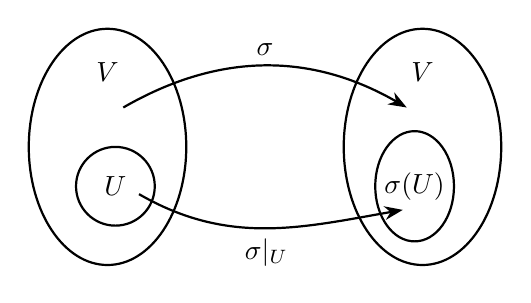
\begin{tikzpicture}[>=Stealth]
        \draw[thick] (-2,0) ellipse (1 and 1.5) node[above=20] {$V$}
        (2,0) ellipse (1 and 1.5) node[above=20] {$V$}
        (-1.9,-0.5) circle (0.5) node {$U$}
        (1.9,-0.5) ellipse (0.5 and 0.7) node {$\sigma(U)$}
        (-1.8,0.5) edge[out=30,in=150,->] node[above] {$\sigma$} (1.8,0.5)
        (-1.6,-0.6) edge[out=-30,in=190,->] node[below] {$\sigma\vert_U$} (1.75,-0.8);
    \end{tikzpicture}
\end{figure}

因此,如果$U$是$\sigma$的不变子空间,根据不变子空间的定义可知,$\sigma\vert_U$就是一个线性变换(是$\mathcal{L}(U)$中的元素),我们称之为\term{限制变换}\index{xianxingyingshe!xianxingbianhuan!xianzhi@限制变换 (restriction operator)}.

有了上面的概念,我们很容易可以将之前的推导转化为以下定理:
\begin{theorem}{}{不变子空间与分块对角矩阵}
    设有限维线性空间$V$上的线性变换$\sigma\in\mathcal{L}(V)$在某组基下的表示矩阵为分块对角矩阵$A=\diag(A_1,\ldots,A_m)$,当且仅当$V$可以分解为不变子空间$U_1,\ldots,U_m$的直和,即
    \[V=U_1\oplus\cdots\oplus U_m,\]
    其中每个$U_i$都是$\sigma$的不变子空间,且$\sigma\vert_{U_i}$在$U_i$对应的基下的表示矩阵为$A_i$.
\end{theorem}

根据定义我们可以验证或者求解一些很简单的不变子空间. 例如设$T\in \mathcal{L}(V)$,则$V$的两个平凡子空间$\{0\}$和$V$,以及映射的像与核$\ker T,\im T$都是$\sigma$不变子空间,验证非常简单,此处不赘述. 事实上当$p$为多项式时,$\ker p(\sigma)$和$\im p(\sigma)$也为$\sigma$的不变子空间. 我们这里也简要书写一下,供读者熟悉如何利用定义验证不变子空间:
\begin{example}{}{多项式不变子空间}
    若$\sigma\in\mathcal{L}(V)$且$p\in\mathbf{F}[x]$为多项式,则$\ker p(\sigma)$和$\im p(\sigma)$在$\sigma$下不变.
\end{example}

\begin{proof}
    我们只需验证$\ker p(\sigma)$和$\im p(\sigma)$中的元素经过$\sigma$映射后仍在这一空间中即可.
    \begin{enumerate}
        \item $\forall \alpha\in \ker p(\sigma),\enspace p(\sigma)\alpha=0$,因此
              \[(p(\sigma))(\sigma(\alpha))=\sigma(p(\sigma)\alpha)=\sigma(0)=0,\]
              即$\sigma(\alpha)\in \ker p(\sigma)$,因此$\ker p(\sigma)$在$\sigma$下不变;

        \item $\forall \alpha\in \im p(\sigma),\enspace \exists \beta\in V,\enspace \alpha=p(\sigma)\beta$,因此
              \[\sigma(\alpha)=\sigma(p(\sigma)\beta)=p(\sigma)(\sigma(\beta))\in \im p(\sigma),\]
              即$\im p(\sigma)$在$\sigma$下不变.
    \end{enumerate}
    事实上,对于$\ker p(\sigma)$,我们有
    \[ p(\sigma)(\alpha)=p(\sigma)\alpha=p(\sigma(\alpha))=p(0)=0,\]
    因此$\sigma(\alpha)\in \ker p(\sigma)$,即$\ker p(\sigma)$在$\sigma$下不变. 对于$\im p(\sigma)$,我们有
    \[\forall \alpha\in \im p(\sigma),\enspace \exists \beta\in V,\enspace \alpha=p(\sigma)\beta,\]
    因此
    \[\sigma(\alpha)=\sigma(p(\sigma)\beta)=p(\sigma)\sigma(\beta)\in \im p(\sigma),\]
    即$\im p(\sigma)$在$\sigma$下不变.
\end{proof}

有时我们可能会遇到更为复杂的情形,如下面的例子:
\begin{example}{}{不变子空间}
    设$\mathbf{F}$为一数域,线性变换$\sigma\in\mathcal{L}(\mathbf{F}^2)$定义为
    \[\sigma(a,b)=(a,b)\begin{pmatrix}
            1 & -1 \\ 2 & 2
        \end{pmatrix}\]
    证明:
    \begin{enumerate}
        \item 当$\mathbf{F}=\mathbf{R}$时,$\mathbf{R}^2$无$\sigma$的非零真不变子空间;

        \item 当$\mathbf{F}=\mathbf{C}$时,$\mathbf{C}^2$有$\sigma$的非零真不变子空间.
    \end{enumerate}
\end{example}

\begin{proof}
    事实上,由于$\sigma$定义在二维空间$\mathbf{F}^2$上,因此``非零真不变子空间''只能是一维子空间. 设该不变子空间$U=\spa(\alpha)(\alpha\neq 0)$,并进一步设$\alpha=(a,b)$. 我们知道,一维线性空间中所有元素都是成比例的(可以理解为一条直线,或者一维空间是由一个向量线性扩张而来,扩张过程中的线性组合一定保证后面生成的所有向量都互相成比例). 我们假设比例值为$\lambda$,即
    \[\sigma(a,b)=(a,b)\begin{pmatrix}
            1 & -1 \\ 2 & 2
        \end{pmatrix}=\lambda(a,b)=(\lambda a,\lambda b),\]
    将矩阵乘法展开,我们有
    \[(a+2b,-a+2b)=(\lambda a,\lambda b).\]
    由于$\alpha=(a,b)\neq 0$,因此$\lambda\neq 0$,基于此解方程得到$\lambda^2-3\lambda+4=0$. 这一方程在实数域范围内无解,复数域内有两个共轭的解,因此,我们有
    \begin{enumerate}
        \item 当$\mathbf{F}=\mathbf{R}$时,$\mathbf{R}^2$无$\sigma$的非零真不变子空间;

        \item 当$\mathbf{F}=\mathbf{C}$时,$\mathbf{C}^2$有$\sigma$的非零真不变子空间.
    \end{enumerate}
\end{proof}

除此之外,还有一些更为困难的问题我们将在讨论完标准形理论之后反过来进行讨论. 为了接下来对标准形讨论的方便,我们需要介绍一个特别的不变子空间:
\begin{definition}{}{循环子空间}
    设$T\in\mathcal{L}(V)$,$v\in V$是一个非零向量. 我们称子空间
    \[W=\spa(v,Tv,T^2v,\ldots,T^kv,\cdots)\]
    为\term{由$v$生成的$T\text{-循环子空间}$}. 在不引起歧义的情况下,我们也称$W$为\term{$T\text{-循环子空间}$}或\term{循环子空间}.
\end{definition}

一个需要注意的地方是,当$V$是有限维线性空间时,循环子空间也一定是有限维的(子空间的维数至少要小于等于原空间). 一个有趣的事实是,如果循环子空间的维数等于$m$,那么它的一组基就是$\{v,Tv,\ldots,T^{m-1}v\}$. 我们来书写这一定理并给出证明:
\begin{theorem}{}{循环子空间}
    设$V$是有限维线性空间,$T\in\mathcal{L}(V)$,$v\in V$是一个非零向量,$W$是由$v$生成的$T-\text{循环子空间}$,则
    \begin{enumerate}
        \item $W$是$T$包含$v$的最小不变子空间;
        \item 若$W$的维数为$m$,则$W$的一组基为$\{v,Tv,\ldots,T^{m-1}v\}$(我们称其为一组循环基).
    \end{enumerate}
\end{theorem}
\begin{proof}
    \begin{enumerate}
        \item 首先我们证明是不变子空间. 由于$V$是有限维线性空间,故$W$一定也是有限维线性空间,故任意的$w\in W$都可以被表示为$W$中有限个元素的线性组合,假设为
              \[w=k_1T^{m_1}v+k_2T^{m_2}v+\cdots+k_sT^{m_s}v,\]
              其中$m_1,m_2,\ldots,m_s\in\mathbf{N}$,$k_1,k_2,\ldots,k_s\in\mathbf{F}$. 我们有
              \[\begin{aligned}
                      Tw & =T(k_1T^{m_1}v+k_2T^{m_2}v+\cdots+k_sT^{m_s}v)     \\
                         & =k_1T^{m_1+1}v+k_2T^{m_2+1}v+\cdots+k_sT^{m_s+1}v,
                  \end{aligned}\]
              因此$Tw$仍然是$W$中向量的线性组合,即$Tw\in W$,故$W$是$T$的不变子空间.

              接下来我们证明是最小不变子空间. 设$U$是$T$的不变子空间,且$v\in U$,我们需要证明$W\subset U$. 由不变子空间的定义以及$v\in U$,我们知道$Tv\in U$,于是进一步利用不变子空间的定义有$T^2v\in U$,以此类推,$T^kv\in U,\enspace\forall k\in\mathbf{N}$,因此$W\subset U$,即$W$是$T$包含$v$的最小不变子空间.

        \item 由于$v$是非零向量,故设$j$是使得$v,Tv,\ldots,T^{j-1}v$线性无关的最大正整数,设$U=\spa(v,Tv,\ldots,T^{j-1}v)$,因此$v,Tv,\ldots,T^{j-1}v$是$U$的一组基. 并且根据我们的假设,$v,Tv,\ldots,T^{j-1}v,T^jv$线性相关,因此根据线性相关性质有
              \[T^jv=k_1v+k_2Tv+\cdots+k_{j-1}T^{j-1}v,\]
              即$T^jv\in U$,于是我们任取$u\in U$,有
              \[u=c_1v+c_2Tv+\cdots+c_{j-1}T^{j-1}v,\]
              因此
              \[Tu=c_1Tv+c_2T^2v+\cdots+c_{j-1}T^jv\in U,\]
              故$U$是$T$的包含$v$的不变子空间. 由定理第一条可知,$W\subset U$,但根据$U$的定义又有$U\subset W$,因此$W=U$,即$W$的一组基为$\{v,Tv,\ldots,T^{j-1}v\}$,故事实上$j$就是$W$的维数. 因此若$W$的维数为$m$,则$W$的一组基为$\{v,Tv,\ldots,T^{m-1}v\}$.
    \end{enumerate}
\end{proof}

最后我们再基于不变子空间讨论一个商线性变换的概念. 事实上,如果$U$是$\sigma$的不变子空间,那么$\sigma$还可以诱导出商空间$V/U$上的线性变换. 定义如下:
\begin{definition}{}{}
    设$\sigma\in \mathcal{L}(V)$,$U$是$\sigma$的不变子空间,定义映射$\sigma/U:V/U\to V/U$如下:
    \[(\sigma/U)(v+U)=\sigma(v)+U,\enspace\forall v\in V,\]
    则称$\sigma/U$是$\sigma$在$U$上的\term{商线性变换}\index{xianxingbianhuan@shang!商线性变换 (quotient operator)}.
\end{definition}

定义映射后,我们自然的想法就失确认这一定义是不是合理的. 首先这一定义的线性性容易验证,我们只需要用到商空间中定义的运算性质即可:
\begin{itemize}
    \item 齐次性:$(\sigma/U)(\lambda(v+U))=(\sigma/U)(\lambda v+U)=\sigma(\lambda v)+U=\lambda\sigma(v)+U=\lambda(\sigma/U)(v+U)$;

    \item 加性:$(\sigma/U)((v_1+U)+(v_2+U))=(\sigma/U)(v_1+v_2+U)=\sigma(v_1+v_2)+U=\sigma(v_1)+\sigma(v_2)+U=(\sigma/U)(v_1+U)+(\sigma/U)(v_2+U)$.
\end{itemize}

除了线性的要求外,还有一个很重要的合理性来源于之前在等价类和商空间中讨论的相容性(或者良定义)的概念,因为这里将线性变换定义在了等价类上. 事实上,对于一个映射,其相容性的关键在于原像集合中的同一个元素只能映射到像集中的唯一一个值(否则不符合映射的定义),具体而言,商线性变换的出发空间元素是等价类,因此如果出现$v+U=w+U$但$\sigma(v)+U\neq \sigma(w)+U$的情况,这一定义描述的就不是映射(因为映射要求一个自变量只能映到一个值上). 我们可以验证这一映射是满足相容性的:

\begin{proof}
    设$v+U=w+U$,即$v-w\in U$,由于$U$在$\sigma$下不变,则$\sigma(v-w)\in U$,即$\sigma(v)-\sigma(w)\in U$,因此$\sigma(v)+U=\sigma(w)+U$,即$\sigma/U$是满足相容性的.
\end{proof}

\section{特征值与特征向量}

在\autoref{thm:不变子空间与分块对角矩阵} 中我们得到了一个很关键的观察,就是不变子空间与分块对角矩阵的关联. 因此我们很自然地希望展开对不变子空间的研究,研究原空间是否能,以及怎么能分解为合理的不变子空间的直和,得到令人满意的简单的矩阵表示. 我们自然需要从最简单的不变子空间开始我们的研究,即一维的不变子空间.

事实上,在\autoref{ex:不变子空间} 中,我们已经尝试求解了一维不变子空间. 根据一维空间中向量都成比例的性质,设$U$是$\sigma\in\mathcal{L}(V)$的一维不变子空间,我们有
\[\exists\lambda\in\mathbf{F},\enspace\sigma(\alpha)=\lambda\alpha,\enspace\forall \alpha\in U,\]
即任意向量作用线性变换后的结果与原向量成比例. 这一性质将引入接下来的特征值与特征向量的概念,事实上它们对于获得简单矩阵的目标而言非常重要,因此是我们讨论的很好的开始.

在接下来的讨论中,我们很多定义和结论都会有相应的矩阵和映射版本. 回顾在\autoref{thm:线性映射对向量坐标的影响} 中的讨论,我们提到了矩阵$A$和线性映射$\sigma(\alpha)=A\alpha$的统一性,并且在相似的引入中我们也提到了我们的目标在线性变换和矩阵两个角度下的陈述及其关联,因此我们未来将不特别区分矩阵和线性变换,这一点在本节过后将有更深刻的体会.

\subsection{特征值与特征向量的定义与求解}

首先介绍线性变换和矩阵的特征值与特征向量的概念:
\begin{definition}{}{}
    设$\sigma$是线性空间$V(\mathbf{F})$上的一个线性变换,如果存在数$\lambda\in\mathbf{F}$和非零向量$\xi\in V$使得$\sigma(\xi)=\lambda\xi$,则称数$\lambda$为$\sigma$的一个\term{特征值}\index{tezhengzhi@特征值 (eigenvalue)},并称非零向量$\xi$为$\sigma$属于其特征值$\lambda$的\term{特征向量}\index{tezhengxiangliang@特征向量 (eigenvector)}.
\end{definition}
必须注意特征向量为非零向量,否则零向量$\xi=\vec{0}$对任意$\lambda$都满足上面定义,从而失去``特征''的含义. 但是特征值可以为0,此时$\sigma(\xi)=\vec{0}$,即全体特征向量的集合就是线性变换的核空间.

对于某一个$\lambda\in\mathbf{F}$,我们将所有满足$\sigma(\xi)=\lambda\xi$的向量构成的集合记为$E(\lambda,\sigma)=\{\xi \mid \sigma(\xi)=\lambda\xi,\enspace\xi\in V\}$(在去除线性变换不引起歧义的情况下可简写为$V_\lambda$),称为$\sigma$关于其特征值$\lambda$的\term{特征子空间}\index{tezhengzikongjian@特征子空间 (eigenspace)}. 显然,这一集合是由零向量和全体$\lambda$对应的特征向量构成的. 我们可以验证$V_\lambda$的确是$V$的``子空间'':
\begin{example}{}{}
    证明:$V_\lambda$是$V$的子空间,并且是线性变换$\sigma$的不变子空间.
\end{example}

\begin{proof}
    回顾证明子空间的两个要求:非空和运算封闭性. 首先$V_\lambda$非空,因为$\vec{0}\in V_\lambda$,即$\sigma(\vec{0})=\lambda\vec{0}$,因此$\vec{0}\in V_\lambda$,故$V_\lambda$非空.

    其次,对于任意$\xi_1,\xi_2\in V_\lambda$,$k_1,k_2\in\mathbf{F}$,我们有
    \[\sigma(k_1\xi_1+k_2\xi_2)=k_1\sigma(\xi_1)+k_2\sigma(\xi_2)=k_1\lambda\xi_1+k_2\lambda\xi_2=\lambda(k_1\xi_1+k_2\xi_2),\]
    因此$k_1\xi_1+k_2\xi_2\in V_\lambda$,故满足线性运算封闭. 综上,$V_\lambda$是$V$的子空间.

    不变子空间也是显然的. 对于任意$\xi\in V_\lambda$,因为$V_\lambda$是由零向量和全体$\lambda$对应的特征向量构成的,因此必有$\sigma(\xi)=\lambda\xi\in V_\lambda$,因此$V_\lambda$是$\sigma$的不变子空间.
\end{proof}

事实上,我们通过之后的例子会知道,$V_\lambda$的维数不一定是1,而至少是1. 那么我们之前引入特征值特征向量时所说的``一维不变子空间''是什么呢?事实上,我们可以取$V_\lambda$的任一组基$\alpha_1,\ldots,\alpha_n$,则其中任一向量进行扩张得到的子空间$U_i=\spa(\alpha_i),\enspace i=1,\ldots,n$就是一维不变子空间,因为$\forall u_i\in U_i,\enspace \sigma(u_i)=\lambda u_i\in U_i$,即$U_i$在$\sigma$下不变. 我们还需要注意,一维不变子空间的选取是不唯一的,因为$V_\lambda$的基的选取是不唯一的,因此$U_i$的选取也是不唯一的,实际上对于任意的$\alpha\in\V_{\lambda}$,$\spa(\alpha)$都是一维不变子空间.

上面是线性变换的特征值与特征向量的定义. 然而我们有一个无法绕开的问题,就是基于线性变换计算特征值与特征向量似乎并不是一个程序化的过程. 因此我们需要求助于矩阵——这是一个适合于计算的良好工具. 对应的,我们给出矩阵的特征值与特征向量的定义:
\begin{definition}{}{}
    设矩阵$A\in \mathbf{M}_n(\mathbf{F})$,如果存在数$\lambda\in\mathbf{F}$和非零向量$X\in\mathbf{F}^n$使得$AX=\lambda X$,则称数$\lambda$为$A$的一个特征值,称非零向量$X$为$A$属于其特征值$\lambda$的特征向量.
\end{definition}

下面我们说明线性映射的特征值与特征向量和矩阵的特征值与特征向量之间的关系. 实际上,假设$A$是$\sigma$在基$\alpha_1,\ldots,\alpha_n$下的表示矩阵,且$\xi=(\alpha_1,\ldots,\alpha_n)X$,即$X$是$\xi$在基$\alpha_1,\ldots,\alpha_n$下的坐标,则我们有
\begin{align*}
    \sigma(\xi)=\lambda\xi & \iff \sigma((\alpha_1,\ldots,\alpha_n)X)=\lambda(\alpha_1,\ldots,\alpha_n)X        \\
                           & \iff (\sigma(\alpha_1,\ldots,\alpha_n))X=(\lambda\alpha_1,\ldots,\lambda\alpha_n)X \\
                           & \iff (\alpha_1,\ldots,\alpha_n)AX=(\alpha_1,\ldots,\alpha_n)(\lambda X)            \\
                           & \iff AX=\lambda X
\end{align*}
其中第一行与第二行间的等价关系用到了矩阵乘法一节中证明的性质$\sigma((\alpha_1,\ldots,\alpha_n)X)=(\sigma(\alpha_1,\ldots,\alpha_n))X$. 由上述讨论可知$\lambda$同时是线性变换和矩阵的特征值,与基的选取无关. 但矩阵的特征向量$X$是线性映射特征向量在基下的坐标,这与基的选取有关. 由于基$\alpha_1,\ldots,\alpha_n$可以是任取的,于是求解线性变换的特征值的问题完全转化为了求线性变换任意一个矩阵表示的特征值,而特征向量也仅仅是向量与坐标的关系. 于是接下来我们讨论如何具体求解特征值与特征向量. 我们首先需要证明一个定理做一个简单的观察:
\begin{theorem}{}{}
    设$\sigma$是$V(\mathbf{F})$上的线性变换,$I$为恒等映射,则下述条件等价:
    \begin{enumerate}[label=(\arabic*)]
        \item \label{item:18:特征值定义:1}
              $\lambda\in\mathbf{F}$是$\sigma$的特征值;

        \item \label{item:18:特征值定义:2}
              $\sigma-\lambda I$不是单射;

        \item \label{item:18:特征值定义:3}
              $\sigma-\lambda I$不是满射;

        \item \label{item:18:特征值定义:4}
              $\sigma-\lambda I$不可逆.
    \end{enumerate}
\end{theorem}

\begin{proof}
    \begin{itemize}
        \item[\ref*{item:18:特征值定义:1}$\implies$\ref*{item:18:特征值定义:2}] $\lambda\in\mathbf{F}$是$\sigma$的特征值,说明$\exists v\in V$且$v\neq 0$使得$\sigma(v)=\lambda v$. 因此$(\sigma-\lambda I)(v)=0$,即$\sigma-\lambda I$核空间不只有零元,根据单射等价条件\autoref{thm:单射与核空间},不单成立;

        \item[\ref*{item:18:特征值定义:2}$\implies$\ref*{item:18:特征值定义:3}] 根据\autoref{thm:双射等价条件} 可知,$\sigma-\lambda I$不满当且仅当$\sigma-\lambda I$不单;

        \item[\ref*{item:18:特征值定义:3}$\implies$\ref*{item:18:特征值定义:4}] 根据\autoref*{thm:双射等价条件} 显然;

        \item[\ref*{item:18:特征值定义:4}$\implies$\ref*{item:18:特征值定义:1}] $\sigma-\lambda I$不可逆,根据\autoref*{thm:双射等价条件} 可知其不为单射,又根据单射等价条件\autoref*{thm:单射与核空间} 可知$(\sigma-\lambda I)(v)=0$有非零解,即$\sigma(v)=\lambda v$,其中$v\neq 0$,这与特征值定义一致.
    \end{itemize}
\end{proof}

由上述定理,$\lambda\in\mathbf{F}$是$\sigma$的特征值等价于$\sigma-\lambda I$不可逆,因此其在$V$的任意一组基$\alpha_1,\ldots,\alpha_n$下的矩阵$A-\lambda E$也不可逆(其中$A$为$\sigma$在这组基下的矩阵,$E$为单位矩阵),这又等价于$|A-\lambda E|=0$.

因此$\lambda\in\mathbf{F}$是$\sigma$的特征值等价于$|\lambda E-A|=0$,故我们可以通过$|\lambda E-A|=0$求解特征值,其中$A$为$\sigma$在某组基下的矩阵,$E$为单位矩阵. 对于特征向量的求解,求出$(\lambda E-A)X=0$的非零解就是特征向量在基$\alpha_1,\ldots,\alpha_n$下的坐标,如果是矩阵的特征向量,那么$X$就是解.

上述求解特征向量的方法需要我们求解$f(\lambda)=|\lambda E-A|$的根,事实上$f(\lambda)=|\lambda E-A|$是在之后的讨论中有核心地位的概念,我们称其为矩阵$A$的\term{特征多项式}{tezhengduoxiangshi@特征多项式 (characteristic polynomial)},其$k$重根称为$k$重特征值(称$k$为代数重数),该特征值对应的特征子空间维数称为该特征值的几何重数.

\begin{example}{}{}
    设$A=\begin{pmatrix}
            1 & -1 & 0 \\ 2 & 0 & 1 \\ 1 & a & 0
        \end{pmatrix}$,且存在非零向量$\alpha$使得$A\alpha=2\alpha$,求$a$.
\end{example}

\begin{solution}
    由题意知2是矩阵$A$的特征值,因此我们有
    \[|2E-A|=\begin{vmatrix}
            1 & 1 & 0 \\ -2 & 2 & -1 \\ -1 & -a & 2
        \end{vmatrix}=9-a=0,\]
    因此$a=9$.
\end{solution}

接下来,我们将特征多项式定义中的行列式展开得到以下定理:
\begin{theorem}{}{特征多项式展开}
    对于$n$级矩阵$A=(a_{ij})$,记
    \[f(\lambda)=|\lambda E-A|=a_0\lambda^n+a_1\lambda^{n-1}+\cdots+a_{n-1}\lambda+a_n\]
    则$a_0=1$,$a_1=-\tr(A)$,$a_n=(-1)^n|A|$,且$a_k$等于所有$k$级主子式之和乘以$(-1)^k$.
\end{theorem}

\begin{proof}
    设$A=(a_{ij})$的列向量为$\alpha_1,\ldots,\alpha_n$,则
    \[f(\lambda)=|\lambda E-A|=\begin{vmatrix}
            \lambda e_1-\alpha_1 & \lambda e_2-\alpha_2 & \cdots & \lambda e_n-\alpha_n
        \end{vmatrix}.\]
    其中$e_1,\ldots,e_n$为$\mathbf{F}^n$的标准基,因此根据行列式的\autoref{def:公理化定义} 的加性,$f(\lambda)$可以拆成$2^n$个行列式的和,它们是
    \begin{equation}\label{eq:18:特征多项式展开}
        (-\alpha_1,\ldots,-\alpha_{j_1-1},\lambda e_{j_1},-\alpha_{j_1+1},\ldots,-\alpha_{j_2-1},\lambda e_{j_2},-\alpha_{j_2+1},\ldots,-\lambda e_{j_{n-k}},\ldots,-\alpha_n),
    \end{equation}
    其中$1\leqslant j_1<j_2<\cdots<j_{n-k}\leqslant n,\enspace k=0,2,\ldots,n$.

    上式初看会显得非常复杂,但实际上利用行列式定义的加性去拆分就是每列有两种拆出来的选择,一种是选择$\lambda e_{j_i}$,另一种是选择$-\alpha_{j_i}$,这就是$2^n$种拆分方式的来由. 其中取出$k$列$-\alpha_{j_i}$,剩余$n-k$列选择$\lambda e_{j_i}$的就可以表示为上式的形式.

    利用\autoref{thm:Laplace定理} 对\autoref{eq:18:特征多项式展开} 第$j_1,\ldots,j_{n-k}$列展开,我们发现这$n-k$列元素组成的$n-k$阶子式只有一个不为0:
    \[\begin{vmatrix}
            \lambda & 0       & \cdots & 0       \\
            0       & \lambda & \cdots & 0       \\
            \vdots  & \vdots  & \ddots & \vdots  \\
            0       & 0       & \cdots & \lambda
        \end{vmatrix}=\lambda^{n-k},\]
    这个不等于0的$n-k$阶子式对应的代数余子式为
    \begin{align*}
         & (-1)^{(j_1+\cdots+j_{n-k})+(j_1+\cdots+j_{n-k})}(-A)
        \begin{pmatrix}
            j_1' & j_2' & \cdots & j_k' \\
            j_1' & j_2' & \cdots & j_k'
        \end{pmatrix}                             \\
         & = (-1)^kA\begin{pmatrix}
                        j_1' & j_2' & \cdots & j_k' \\
                        j_1' & j_2' & \cdots & j_k'
                    \end{pmatrix}
    \end{align*}
    其中$j_1',\ldots,j_k'$为$1,\ldots,n$中除去$j_1,\ldots,j_{n-k}$的$k$个数按递增顺序排列的结果,这一点通过余子式的定义是显然的. 因此\autoref{eq:18:特征多项式展开} 的值为
    \[(-1)^kA\begin{pmatrix}
            j_1' & j_2' & \cdots & j_k' \\
            j_1' & j_2' & \cdots & j_k'
        \end{pmatrix}\lambda^{n-k}.\]
    这实际上只是取$n-k$列$\lambda e_{j_i}$的一种情况,事实上对于所有可能的$j_1,\ldots,j_{n-k}$的取法,我们都可以得到类似的结果,因此$|\lambda E-A|$中$\lambda^{n-k}$的系数为
    \[(-1)^k\sum\limits_{1\leqslant j_1'<\cdots<j_k'\leqslant n}A\begin{pmatrix}
            j_1' & j_2' & \cdots & j_k' \\
            j_1' & j_2' & \cdots & j_k'
        \end{pmatrix}.\]
    即$a_k$等于所有$k$级主子式之和乘以$(-1)^k$,且代入$k=0,1,n$有$a_0=1$,$a_1=-\tr(A)$,$a_n=(-1)^n|A|$.
\end{proof}

这一定理的证明事实上无需掌握,这里给出证明是为了补全教材中的空缺. 这里我们主要掌握两个特例,即由韦达定理,我们有
\begin{enumerate}
    \item $\displaystyle\sum_{i=1}^{n}\lambda_i=\sum_{i=1}^{n}a_{ii}$;

    \item $\displaystyle\prod_{i=1}^{n}\lambda_i=|A|$.
\end{enumerate}
即特征值按重数求和为矩阵的迹(即矩阵对角线元素之和),特征值按重数求积为矩阵行列式. 这一结论在解决某些问题时有一定作用.

事实上,我们这里给出的特征多项式只是矩阵的特征多项式的定义,关于线性变换特征多项式的定义以及进一步讨论将在后续章节进行,我们也会说明两种特征多项式的定义是统一的.

\subsection{相似与特征值、特征向量的关联}
可能细心的读者已经发现,我们前面的讨论中的某个位置留下了一个bug. 我们在讨论线性变换与矩阵的特征值的关联时,提到我们可以取线性变换任意一组基下的表示矩阵来计算特征值,这些特征值就是线性变换的特征值. 事实上这暗示了一个很重要的性质:线性变换任意一组基下的矩阵都有相同的特征值,或者说,相似的矩阵就有相同的特征值,否则上面的讨论一定是有问题的. 我们在此叙述这一性质并给出证明:
\begin{theorem}{}{}
    相似矩阵有相同的特征多项式(逆命题不成立),即$A\sim B$有$|\lambda E-A|=|\lambda E-B|$,从而有相同的迹,行列式,特征值,但特征向量不一定相同.
\end{theorem}
\begin{proof}
    设$B=P^{-1}AP$,则$|\lambda E-B|=|\lambda E-P^{-1}AP|=|P^{-1}(\lambda E-A)P|=|P^{-1}||\lambda E-A||P|=|\lambda E-A|$. 因此$A\sim B$有$|\lambda E-A|=|\lambda E-B|$.

    我们知道特征多项式相同则特征值相同,迹等于所有特征值之和,行列式等于所有特征值之积,因此相似矩阵有相同的迹,行列式,特征值.

    相似矩阵来源于同一线性变换在不同基下的表示,因此它们的特征向量是线性变换的特征向量在不同基下的坐标,因此不一定相同.
\end{proof}

在得到这一结论后,我们同样可以定义线性变换的特征多项式:我们就可以定义其为任意矩阵表示的特征多项式.
\begin{definition}{}{}
    设$\sigma$是$V(\mathbf{F})$上的线性变换,$A$是$\sigma$在任意一组基下的矩阵,则$\sigma$的\term{特征多项式}\index{tezhengduoxiangshi@特征多项式 (characteristic polynomial)}定义为$|\lambda E-A|$.
\end{definition}

下面我们讨论一些重要的例子. 首先要引入的例子也是重要的结论,实际上在行列式一讲中已给出类似结论,但我们现在从特征值角度考虑这一结论:
\begin{example}{}{}
    回答以下两个问题:
    \begin{enumerate}
        \item \label{item:18:特征值相同:1}
              设$A,B$均为$n$阶矩阵,证明:$\lambda\neq 0$是$AB$的特征值,则$\lambda$也是$BA$的特征值;

        \item \label{item:18:特征值相同:2}
              设$A\in \mathbf{M}_{m\times n}(\mathbf{C}),\enspace B\in \mathbf{M}_{n\times m}(\mathbf{C})$,证明:
              \[ \begin{pmatrix}
                      AB & O \\ B & O
                  \end{pmatrix}\sim\begin{pmatrix}
                      O & O \\ B & BA
                  \end{pmatrix} \]
              并由此推出$AB$和$BA$非零特征值相同,且$m=n$时有$|\lambda E-AB|=|\lambda E-BA|$.
    \end{enumerate}
\end{example}

\begin{proof}
    \begin{enumerate}
        \item 设$X$是$AB$属于$\lambda$的特征向量,则$ABX=\lambda X$,因此$B(ABX)=B(\lambda X)$,即$(BA)(BX)=\lambda(BX)$,因此$BX$是$BA$属于$\lambda$的特征向量,故$\lambda$也是$BA$的特征值.

              实际上这里还有一点需要说明,就是$BX\neq 0$,否则它将不能作为特征向量. 事实上证明是简单的,假设$BX=0$,则$ABX=0$,由于$\lambda\neq 0$,因此必然有$X=0$,但这与$X$是$AB$属于$\lambda$的特征向量矛盾,因此$BX\neq 0$.

        \item 根据分块矩阵初等变换的性质,我们可以通过不断尝试选取到$P=\begin{pmatrix}
                      E_m & A \\ O & E_n
                  \end{pmatrix}$,其逆矩阵为$P^{-1}=\begin{pmatrix}
                      E_m & -A \\ O & E_n
                  \end{pmatrix}$,我们发现恰有
              \[\begin{pmatrix}
                      E_m & -A \\ O & E_n
                  \end{pmatrix}\begin{pmatrix}
                      AB & O \\ B & O
                  \end{pmatrix}\begin{pmatrix}
                      E_m & A \\ O & E_n
                  \end{pmatrix}=\begin{pmatrix}
                      O & O \\ B & BA
                  \end{pmatrix}.\]
              因此$\begin{pmatrix}
                      AB & O \\ B & O
                  \end{pmatrix}$与$\begin{pmatrix}
                      O & O \\ B & BA
                  \end{pmatrix}$相似,因此它们的特征多项式相同,即
              \[\begin{vmatrix}
                      \lambda E_m-AB & O \\ -B & \lambda E_n
                  \end{vmatrix}=\begin{vmatrix}
                      \lambda E_m & O \\ -B & \lambda E_n-BA
                  \end{vmatrix}.\]
              根据行列式的计算性质$\begin{vmatrix}
                      A & O \\ C & B
                  \end{vmatrix}=|A||B|$,我们有
              \[|\lambda E_m-AB||\lambda E_n|=|\lambda E_m||\lambda E_n-BA|,\]
              即$\lambda^n|\lambda E_m-AB|=\lambda^m|\lambda E_n-BA|$,因此$AB$和$BA$非零特征值相同,且$m=n$时有$|\lambda E-AB|=|\lambda E-BA|$.
    \end{enumerate}
\end{proof}

不难发现上述例子中 \ref*{item:18:特征值相同:2} 是 \ref*{item:18:特征值相同:1} 的推广,因为由\ref*{item:18:特征值相同:2} 我们得到了$|\lambda E-AB|=|\lambda E-BA|(\lambda\neq 0)$.

下面这个例子非常重要,在解决一些题目时使用这一结论会更便捷:
\begin{example}{}{}
    (\autoref{thm:基的选择对向量坐标的影响} 推广)设$P^{-1}AP=B$,证明:$A,B$分别属于同一特征值$\lambda$的特征向量$X$和$Y$满足$Y=P^{-1}X$.
\end{example}

\begin{proof}
    由$AX=\lambda_0 X$以及$A=PBP^{-1}$,我们有$PBP^{-1}X=\lambda_0 X$,即$BP^{-1}X=\lambda_0 P^{-1}X$,因此$P^{-1}X$是$B$属于$\lambda_0$的特征向量,即$P^{-1}X$是$B$的特征向量,即$Y=P^{-1}X$.
\end{proof}

实际上本题是本讲义\autoref{thm:基的选择对向量坐标的影响} 的推论,原因在于$P^{-1}AP=B$说明$A$和$B$是同一个线性变换(设为$\sigma$)在不同基下的矩阵,因此$X$和$Y$只是$\sigma$关于$\lambda_0$在两组基下的坐标,因此二坐标之间相差一个过渡矩阵.

最后我们谈一个拓展题型,我们考虑矩阵方程$AX-XB=O$,若$A,B$都是$n$阶方阵且$X$可逆,则方程可以改写为$X^{-1}AX=B$,即$A$与$B$相似. 事实上,这一矩阵方程的解空间的维数实际上刻画了$A$与$B$的相似程度. 我们有如下结论:
\begin{theorem}{}{}
    设$A,B$分别为数域$\mathbf{F}$上$n$阶、$m$阶方阵,$A,B$有$r$个两两不等的公共特征值,则矩阵方程$AX-XB=O$有秩为$r$的矩阵解. 反之,若数域为复数域,矩阵方程$AX-XB=O$有秩为$r$的矩阵解,则$A,B$至少有$r$个公共的特征值(计重数).
\end{theorem}

\begin{proof}
    \begin{enumerate}
        \item 设$\lambda_1,\ldots,\lambda_r$是$A$和$B$的$r$个公共特征值,$\alpha_1,\ldots,\alpha_r$为$A$相应的特征向量. 由于$\lambda_1,\ldots,\lambda_r$也是$B^\mathrm{T}$的特征值,设$\beta_1,\ldots,\beta_r$是$B^\mathrm{T}$相应的特征向量. 则$B^\mathrm{T}\beta_i=\lambda_i\beta_i$,从而$\beta_i^{\mathrm{T}}B=\lambda\beta_i^{\mathrm{T}}$. 下面我们证明$X=(\alpha_1,\ldots,\alpha_r)\cdot(\beta_1,\ldots,\beta_r)^\mathrm{T}$是$AX-XB=0$的解.

        事实上,$AX=A(\alpha_1,\ldots,\alpha_r)\cdot(\beta_1,\ldots,\beta_r)^\mathrm{T}=(\lambda_1\alpha_1,\ldots,\lambda_r\alpha_r)\cdot(\beta_1,\ldots,\beta_r)^\mathrm{T}=\lambda_1\alpha_1\beta_1+\cdots+\lambda_r\alpha_r\beta_r$,$XB=(\alpha_1,\ldots,\alpha_r)\cdot(\beta_1,\ldots,\beta_r)^\mathrm{T}B=(\alpha_1,\ldots,\alpha_r)\cdot(\lambda_1\beta_1,\ldots,\lambda_r\beta_r)=(\lambda_1\alpha_1\beta_1+\cdots+\lambda_r\alpha_r\beta_1)$. 故$AX-XB=0$.

        接下来证明$r(X)=r$.
        注意到$r(\alpha_1,\ldots,\alpha_r)=r((\beta_1,\ldots,\beta_r)^\mathrm{T})=r$,故$r(X)\leqslant r(\alpha_1,\ldots,\alpha_r)=r,r(X)\geqslant r(\alpha_1,\ldots,\alpha_r)+r((\beta_1,\ldots,\beta_r)^\mathrm{T})-r$,从而$r(X)=r$.
        \item 设$X=P\begin{pmatrix}
            E_r & 0 \\
            0 & 0
        \end{pmatrix}Q$,则$AX-XB=0$,从而$P^{-1}AP\begin{pmatrix}
            E_r & 0 \\
            0 & 0
        \end{pmatrix} =
        \begin{pmatrix}
            E_r & 0 \\
            0 & 0
        \end{pmatrix}QBQ^{-1}$.

        设$C=P^{-1}AP=\begin{pmatrix}
            C_1 & C_2 \\
            C_3 & C_4
        \end{pmatrix}$,
        $D=QBQ^{-1}=\begin{pmatrix}
            D_1 & D_2 \\
            D_3 & D_4
        \end{pmatrix}$. 则
        $\begin{pmatrix}
            C_1 & C_2 \\
            C_3 & C_4
        \end{pmatrix}\begin{pmatrix}
            E_r & 0 \\
            0 & 0
        \end{pmatrix} = \begin{pmatrix}
            E_r & 0 \\
            0 & 0
        \end{pmatrix}\begin{pmatrix}
            D_1 & D_2 \\
            D_3 & D_4
        \end{pmatrix}$,从而知$C_1=D_1$,$C_2=D_3=0$.
        由于$|\lambda E-C|=|\lambda E_r-C_1||\lambda E_{n-r}-C_4|$,$|\lambda E-D|=|\lambda E_r-D_1||\lambda E_{m-r}-D_4|$,而$|\lambda E_r-C_1|$是一个关于$\lambda$的$r$次多项式,在复数域上有$r$个根(计重数),它们是$C$的特征值,同时也为$D$的特征值. 从而$C$和$D$至少有$r$个公共的特征值. 而相似变换不改变矩阵的特征值,这表明$A,B$至少有$r$个公共的特征值.
    \end{enumerate}
\end{proof}

由此可以看出,复数域上$n$阶、$m$阶方阵$A,B$的矩阵方程$AX=XB$只有零解的充要条件是$A,B$没有公共特征值. 我们通过一个例子应用这一定理:
\begin{example}{}{}
    设$m$阶矩阵$A$与$n$阶矩阵$B$无公共复特征值,$C$为$m\times n$矩阵,则矩阵方程$AX-XB=C$存在唯一解.
\end{example}

\begin{proof}
    设$V$是所有$m\times n$矩阵构成的线性空间,定义$V$上的线性变换$\sigma(X)=AX-XB,\enspace X\in V$. 由于$A$和$B$无公共复特征值,所以$\sigma(X)=AX-XB=O$只有零解,即$\sigma$为$V$上单射,由\autoref{thm:双射等价条件} 可知$\sigma$是满射且是同构映射. 于是,对任意的$C\in V$,都存在唯一的$X_0\in V$使得$\sigma(X_0)=C$,即矩阵方程$AX-XB=C$存在唯一解$X_0$.
\end{proof}

\subsection{特征值的基本性质}

关于特征值,我们有如下基本性质:
\begin{enumerate}
    \item 设$\lambda$是线性空间$V(\mathbf{F})$上的线性变换$\sigma$的特征值,$\xi$是$\sigma$属于$\lambda$的特征向量,则
          \begin{enumerate}
              \item $k\lambda$是$k\sigma$的特征值,$\lambda^m$是$\sigma^m$的特征值,且$\xi$仍是相应特征向量;

              \item 若$f(x)=a_nx^n+a_{n-1}x^{n-1}+\cdots+a_1x+a_0$是$\mathbf{F}$上的多项式,则$f(\sigma)(\xi)=f(\lambda)\xi$;
          \end{enumerate}

    \item 设$\lambda$是$n$阶矩阵$A$的特征值,$A$可逆,则$\lambda^{-1}$是$A^{-1}$的特征值,$|A|\lambda^{-1}$是$A$的伴随矩阵$A^*$的特征值,且特征向量不变.

    \item 设$A$为$n$阶矩阵,则$A$与$A^\mathrm{T}$有相同的特征值(含重数).
\end{enumerate}

\begin{proof}
    \begin{enumerate}
        \item \begin{enumerate}
                  \item 由于$\sigma(\xi)=\lambda\xi$,则$(k\sigma)(\xi)=k\lambda\xi$,即$k\lambda$是$k\sigma$的特征值,$\xi$仍是相应特征向量.

                        而$\sigma^m(\xi)=\sigma^{m-1}(\sigma(\xi))=\sigma^{m-1}(\lambda\xi)=\lambda\sigma^{m-1}(\xi)=\cdots=\lambda^m\xi$,即$\lambda^m$是$\sigma^m$的特征值,$\xi$仍是相应特征向量.

                  \item 利用前述$\sigma^m$的相关性质,我们有
                        \begin{align*}
                            f(\sigma)(\xi) & = (a_n\sigma^n+a_{n-1}\sigma^{n-1}+\cdots+a_1\sigma+a_0I)(\xi)              \\
                                           & = a_n\sigma^n(\xi)+a_{n-1}\sigma^{n-1}(\xi)+\cdots+a_1\sigma(\xi)+a_0I(\xi) \\
                                           & = a_n\lambda^n\xi+a_{n-1}\lambda^{n-1}\xi+\cdots+a_1\lambda\xi+a_0\xi       \\
                                           & = f(\lambda)\xi.
                        \end{align*}
              \end{enumerate}

        \item 设$\xi$是$A$的特征值,即$A\xi=\lambda\xi$,则$\xi=A^{-1}A\xi=A^{-1}\lambda\xi$,即$A^{-1}\xi=\lambda^{-1}\xi$,因此$\lambda^{-1}$是$A^{-1}$的特征值,$\xi$仍是相应特征向量.

              又由于$A$可逆时$A^*=|A|A^{-1}$,根据前面关于$k\sigma$和$A^{-1}$特征值的讨论可知,$|A|\lambda^{-1}$是$A$的伴随矩阵$A^*$的特征值,$\xi$仍是相应特征向量.

        \item 我们用特征多项式证明. 实际上,$A^\mathrm{T}$的特征多项式为$|\lambda E-A^\mathrm{T}|=|(\lambda E-A)^\mathrm{T}|=|\lambda E-A|$(回忆转置不改变行列式),实际上与$A$的特征多项式完全一致,因此$A^\mathrm{T}$与$A$有相同的特征值(含重数).
    \end{enumerate}
\end{proof}

事实上,根据我们之前对线性变换特征值和矩阵特征值的讨论,我们知道上面的结论中``矩阵''和``线性变换''都可以互相替换(除了伴随矩阵没有定义相应的映射).

下面这一例子也是一些经典的结论,应当熟悉.
\begin{example}{}{特征值的性质}
    对下列矩阵$A$的特征值,能做出怎样的断言?
    \begin{enumerate}
        \item $A$可逆/$A$不可逆/$E+A$可逆/$4E+A$不可逆;

        \item $|E-A^2|=0$;

        \item $A^2=E$(对合)/$A^2=A$(幂等)/$A^k=0$(幂零);

        \item $A=\lambda_0E+B$($\lambda_0$为常数,且已知$B$的$n$个特征值为$\lambda_1,\lambda_2,\ldots,\lambda_n$);

        \item $A$为对角块矩阵,即$A=\diag(A_1,A_2,\ldots,A_m)$.
    \end{enumerate}
\end{example}

\begin{solution}
    \begin{enumerate}
        \item $A$可逆时有$|A|=\lambda_1\cdots\lambda_n\neq 0$,因此$A$的特征值都不为0. 同理,$A$不可逆同理表明存在特征值等于0,$E+A$可逆表明$-1$不是$A$的特征值,$4E+A$不可逆表明$-4$是$A$的特征值.

        \item $|E-A^2|=|E-A||E+A|=0$,因此$\pm 1$都是$A$的特征值.

        \item 我们首先考虑对合矩阵,接下来的同理可以得到类似结论. 由于$A^2=E$,设$AX=\lambda X$,则$A^2X=\lambda^2X=X$,因此$\lambda^2=1$,即$\lambda=\pm 1$,因此$1$或$-1$是$A$的特征值.

              但这里我们需要强调的是,不同于前两问,前两问中我们都是说某些值是$A$的特征值,但无法保证$A$的特征值只能是某些值,但在本题这样给出矩阵方程的情况下,我们可以得到$A$的特征值只能是$\pm 1$,没有其他值. 我们用反证法,假设存在$\lambda_0\neq\pm 1$是$A$的特征值,即$AX=\lambda_0X$,则$A^2X=\lambda_0^2X\neq X$(因为$X$不是零向量),导出矛盾. 当然有同学可能会思考,$A$的特征值一定兼有$\pm 1$吗,事实上并非如此,例如$E$满足$E^2=E$,但其特征值只有1,$-E$满足$(-E)^2=E$,但其特征值只有$-1$. 并且利用下一讲对角化的结论可以知道(我们放在下一讲习题中供读者练习),满足$A^2=E$且特征值只有1的矩阵只能是$E$,特征值只有$-1$的矩阵只能是$-E$.

              注:本题解决过程中告诉我们一个解题技巧,如果看到$A$的多项式$f(A)=O$这种形式的表达式,事实上$A$的特征值只能是$f(\lambda)=0$的根,如上题中$f(A)=A^2-E$,则$f(\lambda)=\lambda^2-1$,因此$A$的特征值只能是$\pm 1$.

              同理,我们可以知道幂等矩阵的特征值只能是0和1,幂零矩阵的特征值只能是0(这是一个重要的幂零矩阵等价条件,未来我们会再次遇到).

        \item 设$BX=\lambda_iX_i(X_i\neq 0,\enspace i=1,\ldots,n)$,则$AX_i=\lambda_0X_i+BX_i=\lambda_0X_i+\lambda_iX_i=(\lambda_0+\lambda_i)X_i$,因此$\lambda_0+\lambda_i\enspace(i=1,\ldots,n)$都是$A$的特征值.

        \item \begin{align*}
                  |\lambda E-A| & =\begin{vmatrix}
                                       \lambda E_1-A_1 & 0               & \cdots & 0               \\
                                       0               & \lambda E_2-A_2 & \cdots & 0               \\
                                       \vdots          & \vdots          & \ddots & \vdots          \\
                                       0               & 0               & \cdots & \lambda E_m-A_m
                                   \end{vmatrix}
                                & =\prod_{i=1}^{m}|\lambda E_i-A_i|=0
              \end{align*}
              因此,$A_i,\enspace i=1,\ldots,m$的特征值都是$A$的特征值.
    \end{enumerate}
\end{solution}

当然在本题中,我们看到了一些特殊的矩阵,如对合矩阵,幂等矩阵,幂零矩阵等,我们在之后还会讨论它们的一些性质,特别是幂等矩阵和幂零矩阵,因此我们很有必要为这些矩阵写下一个定义. 当然这些名词还有对应的线性变换版本,下面我们给出正式的定义:
\begin{definition}{}{}
    一个矩阵$A$(或线性变换$\sigma$)称为\textbf{对合矩阵}(或\textbf{对合变换}),如果$A^2=E$(或$\sigma^2=I$);称为\textbf{幂等矩阵}(或\textbf{幂等变换}),如果$A^2=A$(或$\sigma^2=\sigma$);称为\textbf{幂零矩阵}(或\textbf{幂零变换}),如果存在自然数$k$使得$A^k=O$(或$\sigma^k=O$).
\end{definition}

基于上面给出的性质和例子,我们可以进一步运用特征值的性质来求解一些问题,下面是一些例子:
\begin{example}{}{}
    回答以下问题:
    \begin{enumerate}
        \item 设$\alpha=(1,0,-1)^\mathrm{T}$,且$A=\alpha\alpha^\mathrm{T}$,求$|6E-A^n|$;

        \item 设$A$为三阶矩阵,其特征值为$1,-2,-1$,求$|A|$,$A^*+3E$的特征值,$(A^{-1})^2+2E$的特征值以及$|A^2-A+E|$;

        \item 设$A$为三阶矩阵,$A^2-A-2E=O$,$|A|=2$,求$|A^*+3E|$;

        \item 设$A$为三阶矩阵,其特征值为$-1,-1,5$,求$A_{11}+A_{22}+A_{33}$;
    \end{enumerate}
\end{example}

\begin{solution}
    \begin{enumerate}
        \item 事实上$A=\alpha\alpha^\mathrm{T}=\begin{pmatrix}
                      1 & 0 & -1 \\ 0 & 0 & 0 \\ -1 & 0 & 1
                  \end{pmatrix}$,由$|\lambda E-A|=0$解得$A$的特征值为$\lambda_1=\lambda_2=0,\lambda_3=2$,而根据$A^n$的特征值性质和\autoref{ex:特征值的性质} 可知,$6E-A^n$的特征值为$6-\lambda_1^n,6-\lambda_2^n,6-\lambda_3^n$,即$6,6,6-2^n$,因此$|6E-A^n|=6^2(6-2^n)=36(6-2^n)$.

        \item 由于$A$的特征值为$1,-2,-1$,因此$|A|=1\times(-2)\times(-1)=2$,而$A^*$的特征值为$|A|\lambda^{-1}$,因此$A^*$的特征值为$2,-1,-2$,故$A^*+3E$的特征值为$A^*$的特征值加3(根据\autoref{ex:特征值的性质}),即为$5,2,1$,又根据$A^{-1}$和$A^2$特征值的性质可知,$(A^{-1})^2+2E$的特征值为$1^2+2,(-1/2)^2+2,(-1)^2+2$,即为$3,9/4,3$,而$A^2-A+E$的特征值根据$f(\sigma)$特征值性质的讨论可知为$1^2-1+1,(-2)^2-(-2)+1,(-1)^2-(-1)+1$,即为$1,7,3$,因此$|A^2-A+E|=1\times 7\times 3=21$.

        \item 设$AX=\lambda X(X\neq 0)$,则$(A^2-A-2E)X=(\lambda^2-\lambda-2)X=O$,因此$\lambda=-1$或$\lambda=2$,根据\autoref{ex:特征值的性质} 中关于对合矩阵的讨论可知,$A$的特征值恰为-1和2. 又$|A|=2$,且$A$为3阶矩阵,因此$A$的3个特征值必为-1,-1,2.

              又$A^*$的特征值为$|A|\lambda^{-1}$,因此$A^*$的特征值为$1,-2,-2$,又根据\autoref{ex:特征值的性质} 的结论,$A^*+3E$的特征值为$A^*$的特征值加3,即$\lambda_1=\lambda_2=1,\lambda_3=4$,故$|A^*+3E|=\lambda_1\lambda_2\lambda_3=4$.

        \item 由题意知$|A|=5$,故$A^*$的特征值为$|A|\lambda^{-1}$即为$\mu_1=\mu_2=-5,\mu_3=1$,而$A_{11}+A_{22}+A_{33}$就是$A^*$的迹(即矩阵对角线元素之和),因此$A_{11}+A_{22}+A_{33}=\mu_1+\mu_2+\mu_3=-9$.
    \end{enumerate}
\end{solution}

\subsection{特征向量的基本性质}

这一部分的定理与下一讲中得到简单矩阵的可对角化的等价条件直接相关,实际上有了本节的定理,可对角化条件是很显然的.
\begin{theorem}{}{特征向量的基本性质}
    设$V$是有限维的,$\sigma\in L(V)$且$\lambda\in\mathbf{F}$,则
    \begin{enumerate}
        \item $\sigma$的不同特征值对应的特征向量线性无关;

        \item $\sigma$的不同特征值对应的特征子空间的和为直和;

        \item $\sigma$最多有$\dim V$个不同的特征值.
    \end{enumerate}
\end{theorem}

\begin{proof}
    \begin{enumerate}
        \item 设$\lambda_1,\ldots,\lambda_m$是$\sigma$的互异特征值,$\xi_1,\ldots,\xi_m$是相应的特征向量. 反证法,我们假设$\xi_1,\ldots,\xi_m$线性相关,由\autoref{lem:线性相关性引理} 可知,存在$k$是使得
              \[\xi_k\in\spa(\xi_1,\ldots,\xi_{k-1})\]
              成立的最小整数,则存在$c_1,\ldots,c_{k-1}$使得
              \begin{equation}\label{eq:18:特征向量线性无关}
                  \xi_k=c_1\xi_1+\cdots+c_{k-1}\xi_{k-1}.
              \end{equation}
              将$\sigma$作用到上式两边,我们有
              \[\lambda_k\xi_k=c_1\lambda_1\xi_1+\cdots+c_{k-1}\lambda_{k-1}\xi_{k-1}.\]
              将\autoref{eq:18:特征向量线性无关} 两边乘以$\lambda_k$,然后减去上式,我们有
              \[0=c_1(\lambda_k-\lambda_1)\xi_1+\cdots+c_{k-1}(\lambda_k-\lambda_{k-1})\xi_{k-1}.\]
              由于我们选取的$k$是满足$\xi_k\in\spa(\xi_1,\ldots,\xi_{k-1})$的最小整数,因此$\xi_1,\ldots,\xi_{k-1}$线性无关,故$a_1=\cdots=a_{k-1}=0$,因此$\xi_k=0$,这与$\xi_k$是特征向量矛盾,因此$\xi_1,\ldots,\xi_m$线性无关.

        \item 回忆直和的证明方法,我们在\autoref{thm:直和等价命题} 中选取合适等价命题进行证明. 假设
              \begin{equation}\label{eq:18:特征子空间直和}
                  \xi_1+\cdots+\xi_m=0,
              \end{equation}
              其中$\xi_i\in V_{\lambda_i}$,由于$\sigma$的不同特征值对应的特征向量线性无关,因此$\xi_1,\ldots,\xi_m$不可能是特征向量,否则由\autoref{eq:18:特征子空间直和} 可知它们线性相关,故必有$\xi_1=\cdots=\xi_m=0$,这表明$\sigma$的不同特征值对应的特征子空间的和为直和.

        \item 设$\lambda_1,\ldots,\lambda_m$是$\sigma$的互异特征值,$\xi_1,\ldots,\xi_m$是相应的特征向量. 前面已经证明了$\xi_1,\ldots,\xi_m$线性无关,因此$\dim V\geqslant m$,得证.
    \end{enumerate}
\end{proof}

上述定理有如下推论:
\begin{enumerate}
    \item 若$\lambda_1,\ldots,\lambda_m$是线性映射$\sigma$互异的特征值,则$V_{\lambda_i}\cap\sum\limits_{j\neq i}V_{\lambda_j}=\{0\}
              \enspace(i=1,\ldots,m)$,则一个特征向量不能属于多个特征值. 这一推论来源于直和的一个等价条件,线性空间运算一讲的习题中有涉及.

    \item $\sigma$的不同特征值$\lambda_1,\ldots,\lambda_m$对应的特征子空间$V_{\lambda_1},\ldots,V_{\lambda_m}$的基向量合在一起构成的向量组线性无关,且是$V_{\lambda_1}+V_{\lambda_2}+\cdots+V_{\lambda_m}$的基.
\end{enumerate}

接下来这个定理讨论了代数重数和几何重数间的关系:
\begin{theorem}{}{代数重数与几何重数}
    $n$维线性空间$V(\mathbf{F})$的线性变换$\sigma$的每个特征值$\lambda_0$的重数(代数重数)大于等于其特征子空间$V_{\lambda_0}$的维数(几何重数).
\end{theorem}

\begin{proof}
    根据线性变换和矩阵特征值的统一性(即特征多项式一致,故特征值代数重数一致)以及特征向量通过坐标映射一一对应的性质(即几何重数一致),我们只需要讨论$\sigma$在$V$的某一组基下的表示矩阵$A$的情况即可.

    设$\lambda_0$对应的特征子空间维数为$r$,则存在$V_{\lambda_0}$的一组基$\xi_1,\ldots,\xi_r$,并将其扩充为$V$的一组基$\xi_1,\ldots,\xi_r,\xi_{r+1},\ldots,\xi_n$.

    定义$n$阶可逆矩阵$U=(\xi_1,\ldots,\xi_r,\xi_{r+1},\ldots,\xi_n)$,根据$A\xi_i=\lambda_0\xi_i\enspace(i=1,\ldots,r)$,我们有
    \begin{align*}
        A(\xi_1,\ldots,\xi_r,\xi_{r+1},\ldots,\xi_n) & = (\lambda_0\xi_1,\ldots,\lambda_0\xi_r,A\xi_{r+1},\ldots,A\xi_n) \\
                                                     & = (\xi_1,\ldots,\xi_r,\xi_{r+1},\ldots,\xi_n)
        \begin{pmatrix}
            \lambda_0 E_r & B \\ O & C
        \end{pmatrix}
    \end{align*}
    其中$B$是$r\times(n-r)$矩阵,$C$是$(n-r)\times(n-r)$矩阵,$O$是零矩阵. 记$D=\begin{pmatrix}
            \lambda_0 E_r & B \\ O & C
        \end{pmatrix}$,则$AU=UD\implies A=UDU^{-1}$.

    考虑特征多项式$|\lambda E-A|=|\lambda E-UDU^{-1}|=|U(\lambda E_n-D)U^{-1}|=|U||\lambda E_n-D||U^{-1}|=|\lambda E_n-D|$,故$|\lambda E-A|=|\lambda E_n-D|$. 进一步地,$|\lambda E-D|=|\lambda E_r-\lambda_0 E_r||\lambda E_{n-r}-C|=(\lambda-\lambda_0)^r|\lambda E_{n-r}-C|$,因此$\lambda_0$作为特征多项式$|\lambda E-A|$的根的重数至少为$r$,即$\lambda_0$的代数重数大于等于其特征子空间$V_{\lambda}$的维数.
\end{proof}

事实上,由于$n$阶矩阵的特征多项式是$n$次的,因此所有特征值的代数重数之和等于$n$,但是根据上述定理可知所有特征值的几何重数之和小于等于$n$,即所有特征子空间的直和不一定能够得到原空间$V$. 这将构成我们接下来讨论的一个核心:我们在下一讲中将要讨论代数重数和几何重数相等情况下的最简单的矩阵表示,以及二者不相等的时候如何对原空间进行分解(因为此时$V$不能被分解为特征子空间直和)使得我们可以获得较为简单的矩阵表示.

最后我们再通过一个例子体会特征向量和特征子空间的一些性质:
\begin{example}{}{}
    设$V(\mathbf{F})$是$n$维线性空间,$\sigma\in \mathcal{L}(V)$,证明:
    \begin{enumerate}
        \item 若$\alpha,\beta$是$\sigma$的属于不同特征值的特征向量,则$c_1c_2\neq 0$时,$c_1\alpha+c_2\beta$不是$\sigma$的特征向量;

        \item $V$中的每一非零向量都是$\sigma$的特征向量$\iff\sigma=c_0I_V$,其中$c_0\in\mathbf{F}$是一个常数,$I_V$是恒等变换.
    \end{enumerate}
\end{example}

\begin{proof}
    \begin{enumerate}
        \item 设$\sigma(\alpha)=\lambda_1\alpha,\sigma(\beta)=\lambda_2\beta$,其中$\lambda_1\neq\lambda_2$,并假设$c_1\alpha+c_2\beta$是$\sigma$的特征向量,即存在$\lambda_0\in\mathbf{F}$使得
              \[\sigma(c_1\alpha+c_2\beta)=\lambda_0(c_1\alpha+c_2\beta).\]
              展开括号,我们有
              \[c_1\sigma(\alpha)+c_2\sigma(\beta)=c_1\lambda_0\alpha+c_2\lambda_0\beta.\]
              即$c_1\lambda_1\alpha+c_2\lambda_2\beta=c_1\lambda_0\alpha+c_2\lambda_0\beta$,即$(\lambda_1-\lambda_0)c_1\alpha+(\lambda_2-\lambda_0)c_2\beta=0$,由于$\alpha,\beta$线性无关,因此
              \[c_1(\lambda_1-\lambda_0)=c_2(\lambda_2-\lambda_0)=0.\]
              当$c_1c_2\neq 0$时,我们有$\lambda_1=\lambda_0=\lambda_2$,这与$\lambda_1\neq\lambda_2$矛盾,因此$c_1\alpha+c_2\beta$不是$\sigma$的特征向量.

        \item 右推左显然,我们只考虑左推右的证明. 由上一小问结论可知,若$V$中的每一非零向量都是$\sigma$的特征向量,$\sigma$不可能有不同的特征值(因为有不同的特征值就有不同特征值对应的特征向量,但它们的线性组合一定仍在$V$中,这与从第一问中得到的结论,即它不是$\sigma$的特征向量矛盾). 设$c_0$是$\sigma$的唯一的特征值,则对于任意$\alpha\in V$,我们有$\sigma(\alpha)=c_0\alpha$,即$\sigma$在任意元素上的像都已经唯一确定,则显然在$V$的一组基上的像也唯一确定,由\autoref{thm:线性映射唯一确定} 可知这样的线性映射是唯一的,$\sigma=c_0I_V$符合要求,因此它就是我们要找的线性映射.
    \end{enumerate}
\end{proof}

事实上,本题的结论是十分具有启发性的. 它表明,即便所有特征子空间的直和等于全空间$V$,这也不表明$V$中所有向量都是特征向量,只有特征值唯一时才能做到这一点. 原因在于不同特征子空间之间是直和,因此我们无法通过两个特征子空间的基向量的线性组合(系数非零)来得到任意特征子空间中的向量,相反,这样的线性组合会使得得到的新向量不在任何一个特征子空间中,因此无法使得$V$中所有向量都是特征向量.

下面我们通过一个例子给出一种由特征向量出发生成线性无关向量组的方法,这一例子将在后续的讨论中起到重要作用:
\begin{example}{}{特征向量生成线性无关组}
    设 $A$ 是数域 $\mathbf{F}$ 上一个 $n$ 阶方阵,$E$ 是 $n$ 阶单位矩阵,$\alpha_1 \in \mathbf{F}^n$ 是 $A$ 的属于特征值 $\lambda$ 的一个特征向量,向量组 $\alpha_1,\alpha_2,\ldots,\alpha_s$ 按如下方式产生:$(A-\lambda E)\alpha_{i+1}=\alpha_i,\enspace i=1,2,\ldots,s-1$. 证明向量组 $\{\alpha_1,\alpha_2,\ldots,\alpha_s\}$ 线性无关.
\end{example}

\begin{proof}
    由于$\alpha_1$是$A$属于特征值$\lambda$的特征向量,故有$(A-\lambda E)\alpha_1=0$.

    设$\displaystyle\sum_{i=1}^{s}k_i\alpha_i=0$,两边同时左乘$A-\lambda E$可知$(A-\lambda E)\displaystyle\sum_{i=1}^{s}k_i\alpha_i=\displaystyle\sum_{i=1}^{s}k_i(A-\lambda E)\alpha_i=k_1(A-\lambda E)\alpha_1+\displaystyle\sum_{i=1}^{s-1}k_{i+1}\alpha_i=\displaystyle\sum_{i=1}^{s-1}k_{i+1}\alpha_i=0$.

    以此类推,在等式两边不断左乘$(A-\lambda E)$可知:对于$\forall r \in \{1,\cdots,s-1\}$都有$\displaystyle\sum_{i=1}^{s-r}k_{i+r}\alpha_i=0$.

    令$r=s-1$得到$k_s\alpha_1=0,k_s=0$. 再依次代回不难得到$k_i=0,\forall i \in \{1,\cdots,s\}$,从而向量组$\alpha_1,\cdots,\alpha_s$线性无关.
\end{proof}

\section{实数域与复数域的讨论}

在上一节中我们并没有明确区分特征值所在的数域(即线性空间$V$定义的数域). 实际上上面的讨论都是与数域无关的,即无论是什么数域上面的定理都是成立的. 然而,从\autoref{ex:不变子空间} 中我们看到实数域和复数域可能有本质的不同,即特征值的存在性可能存在差别. 事实上,这是\nameref{thm:多项式的唯一分解定理}的必然结果,因为复数域上$n$次多项式一定有$n$个根,但实数域上可能根会减少,因此$n$次特征多项式$f(\lambda)$在实数域上解的情况与复数域有差别.

因此我们有必要分别讨论在复数域和实数域条件下特征值与特征向量的不同性质,事实上我们将在实空间上的线性变换一讲中单独深入讨论这一主题,但现在我们需要几个定理来引入这一话题并为接下来的讨论作准备:
\begin{theorem}{}{复数域上的特征值}
    设$\sigma\in \mathcal{L}(V)$,$V$是$n$维复线性空间,则$\sigma$必有特征值.
\end{theorem}

这一定理从解特征多项式求特征值的角度来看是非常显然的,因为此时特征多项式$f(\lambda)$展开后为$n$次多项式,则由代数学基本定理,$f(\lambda)=0$在复数域上有$n$个解,因此复线性空间上的线性变换一定有特征值. 注意实线性空间上不一定有特征值,因为$f(\lambda)=0$可能无实根.

这一命题也可以不使用特征多项式解决,下面我们给出一种不使用行列式、特征多项式的证明方法:
\begin{proof}
    对于$v \in V,v \neq 0$,$v,\sigma(v),\cdots,\sigma^n(v)$线性相关,从而存在不全为$0$的复数$a_0,a_1,\cdots,a_n$,使得$a_0v+a_1\sigma(v)+\cdots+a_n\sigma^n(v)=0$. 由于$v \neq 0$,故$a_1,\cdots,a_n$不全为$0$.

    令$f(z)=\displaystyle\sum_{i=0}^{n}a_iz^i=c\displaystyle\prod_{i=1}^{m}(z-\lambda_i)$,则$0=f(\sigma)(v)=c(\sigma-\lambda_1I)\cdots(\sigma-\lambda_mI)v$,这表明$\exists j\in \{1,\cdots,m\}$使得$(\sigma-\lambda_jI)$不是单的,从而$\sigma$有本征值.
\end{proof}
当然还有很多不同的证明方法,此处篇幅有限不再赘述.

\begin{theorem}{}{特征值与不变子空间}
    任取$\sigma\in \mathcal{L}(V)$,$V$是$n$维线性空间(无论数域是实或复),则$\sigma$一定有一维或二维不变子空间.
\end{theorem}

\begin{proof}
    由\autoref{thm:复数域上的特征值} 可知,复空间$\sigma$有特征值$\lambda$,因此根据在特征子空间的讨论可知必然存在一维不变子空间.

    若$\sigma$定义在实空间上,我们可以首先考虑复数域上的特征值,若$a+b\i$是$\sigma$的特征值,其中$a,b\in\mathbf{R}$,则存在不全为零的实向量$\alpha,\beta$使得$\alpha+\beta\i$是$\sigma$的特征向量,即我们有
    \[\sigma(\alpha+\beta\i)=(a+b\i)(\alpha+\beta\i).\]
    展开括号,我们可以得到
    \[\sigma(\alpha)=a\alpha-b\beta,\sigma(\beta)=b\alpha+a\beta.\]
    令$U=\spa(\alpha,\beta)$,则$U$是$\sigma$的不变子空间,且$\dim U=1$或$\dim U=2$,具体取值取决于$\alpha$和$\beta$是否线性相关.
\end{proof}

这里讨论实空间的情况时,我们用到了一个很特别的思想,即首先考虑了复特征值和特征向量,然后通过将复数表示为$a+b\i(a,b\in\mathbf{R})$的形式转回了实空间上的研究. 这一思想我们称之为``复化'',我们将在本讲义后面的章节中更为完整地讨论这一思想.

最后我们讨论实数特征值和复数特征值几何意义的不同. 比较显然的一点是,实数域上的特征值与特征向量的几何意义在于,某一线性变换的特征向量在经过变换后得到的向量与原先向量共线,因为若$\alpha\in V$为$\sigma$的特征向量,则存在$\lambda\in\mathbf{R}$有$\sigma(\alpha)=\lambda\alpha$,因此$\alpha$被线性变换作用后相当于简单的按比例伸缩.

但是如果特征值是复数,那么情况并不会这么简单. 我们接下来的讨论思路比较直观,不够严谨,但是可以帮助我们理解复数特征值的几何意义. 我们首先来看一个例子:
\begin{example}{}{}
    设$\sigma\in\mathcal{L}(\mathbf{F}^2)$定义为$\sigma(w,z)=(-z,w)$.
    \begin{enumerate}
        \item 当$\mathbf{F}=\mathbf{R}$时,求$\sigma$的特征值和特征向量;

        \item 当$\mathbf{F}=\mathbf{C}$时,求$\sigma$的特征值和特征向量.
    \end{enumerate}
\end{example}

\begin{solution}
    我们首先写出$\sigma$在任意一组基下的矩阵表示,为了方便,我们选取标准基$e_1=(1,0),e_2=(0,1)$,则矩阵表示为
    \[ A=\begin{pmatrix}
            0 & -1 \\ 1 & 0
        \end{pmatrix}. \]
    则其特征多项式$f(\lambda)=|\lambda E-A|=\lambda^2+1$,因此
    \begin{enumerate}
        \item 在实数域上无特征值和特征向量;

        \item 复数域上特征值为$\pm\i$,其中$\i$对应的特征向量为$(w,-wi)$,$-\i$对应的特征向量为$(w,wi)$,其中$w\in\mathbf{R}$且$w\neq 0$.
    \end{enumerate}
\end{solution}

这里需要强调的一点是,$\mathbf{C}^2$也是二维线性空间,原因在于这里的$\mathbf{C}^2$的含义是定义在复数域上的,即是$\mathbf{C}^2(\mathbf{C})$,而不是$\mathbf{C}^2(\mathbf{R})$,因此维数为2而非4. 事实上在\autoref{ex:不同数域的维数} 中读者应当就已经理解了这一点,此处不再做详细解释.

事实上,我们可以抛开程序式的解题步骤,仔细观察这里的映射定义,我们会发现,在实数域内这一变换$\sigma$就是二维平面中将向量绕原点逆时针旋转90$^\circ$的旋转变换,因此在实数域内无特征值(实特征值实际上只能将特征向量沿着原方向伸缩). 但为何复数域内有特征值呢?我们回忆复数的极坐标表示,任意复数$z$可表示为$z=re^{\i\theta}$,因此直观而言复特征值除了伸缩效应外也有旋转的效应.

本题中两个特征向量可以写为$\alpha\pm \i\beta$,则$T$在$(\alpha,\beta)$这组基下的矩阵表示就是一个表示旋转90$^\circ$的矩阵乘以单位矩阵(表明伸缩为比例1),这表明线性变换对空间的伸缩作用与特征值模长对应,旋转作用与辐角对应(本题特征值$\pm \i=1\cdot(\cos 90^\circ\pm \i\sin 90^\circ)$).

我们还可以延伸到三维空间. 设三阶矩阵$A=(a_{ij})_{3\times 3}$,设这一矩阵有三个互异特征值,则根据多项式的性质可知,其中两个为共轭复数$\lambda_{1,2}=a\pm b$,还有一个实数$\lambda_3=c$,对应的特征向量为$v_{1,2}=\alpha\pm \i\beta,v_3=\gamma$,则$T$在$\alpha,\beta,\gamma$下的矩阵表示为
\[ B=\begin{pmatrix}
        a & b & 0 \\ -b & a & 0 \\ 0 & 0 & c
    \end{pmatrix}, \]
我们令$r=\sqrt{a^2+b^2},a=r\cos\theta,b=r\sin\theta$,则有
\[ B=\begin{pmatrix}
        \cos\theta & -\sin\theta & 0 \\ \sin\theta & \cos\theta & 0 \\ 0 & 0 & 1
    \end{pmatrix}\begin{pmatrix}
        r & 0 & 0 \\ 0 & r & 0 \\ 0 & 0 & c
    \end{pmatrix}. \]
我们可以看到,这个变换被分解为两个变换,一个是在$x-y$平面上的旋转,另一个是拉伸,在$x-y$平面上拉伸$r$倍,$z$方向拉伸$c$倍. 这显然是二维结论的自然推广.

在更高维的情况也是类似的,矩阵也可以表示为一个旋转向量的矩阵乘以一个伸缩向量的矩阵,旋转角度是复特征值的辐角,伸缩倍数是复特征值的模长.

\section{特征值的估计}

对于低阶的矩阵来说,我们可以通过解特征多项式来精确求得特征值;但对于高阶矩阵而言,解特征多项式是非常困难的,所幸相关的工作一般来说也不需要我们精确求得特征值,所以我们可以通过一些方法来估计特征值.

\begin{definition}{Gershgorin 圆盘}{Gershgorin disks}
    设 $T \in \mathcal{L}(V)$,并且 $v_1, \ldots, v_n$ 是 $V$ 的一组基,$A = (a_{ij})_{n \times n}$ 为 $T$ 在这组基下的矩阵表示. 那么 $T$ 关于这组基的一个 Gershgorin 圆盘是指如下形式的集合:
    \[ D_i = \left\{z \in \mathbf{F} \mid \lvert z - a_{ii} \rvert \leqslant \sum_{j \neq i} \lvert a_{ij} \rvert\right\}, i = 1, \ldots, n. \]
\end{definition}

因为有 $n$ 个对角元可供选择,所以 $T$ 共有 $n$ 个 Gershgorin 圆盘. 在复数域考虑的话,上述的 $D_i$ 就是闭圆盘,而在实数域考虑的话,$D_i$ 就是闭区间.

在进一步讨论之前,先考虑一种特殊的情况:对角矩阵. 设 $T \in \mathcal{L}(V)$,并且 $v_1, \ldots, v_n$ 是 $V$ 的一组基,$A = (a_{ij})_{n \times n}$ 为 $T$ 在这组基下的矩阵表示. 若 $A$ 是对角矩阵,那么 $T$ 相应的 Gershgorin 圆盘就是 $n$ 个单点,也就是对应的特征值. 这让我们朦胧之中觉得 Gershgorin 圆盘或许可以“控制”特征值. 事实上,这一想法是正确的:

\begin{theorem}{Gershgorin 圆盘第一定理}{Gershgorin disks theorem}
    设 $T \in \mathcal{L}(V)$,并且 $v_1, \ldots, v_n$ 是 $V$ 的一组基. 那么 $T$ 的每个特征值都在其关于 $v_1, \ldots, v_n$ 这组基的某个 Gershgorin 圆盘内.
\end{theorem}

\begin{proof}
    设 $\lambda \in \mathbf{F}$ 是 $T$ 的一个特征值,$w \in V$ 是对应的一个特征向量,所以存在 $c_1,\ldots, c_n \in \mathbf{F}$ 使得
    \[
        w = c_1 v_1 + \cdots + c_n v_n.
    \]
    设 $A$ 是 $T$ 关于 $v_1, \ldots, v_n$ 这组基的矩阵表示,对上式两侧同时作用 $T$,便有
    \begin{align*}
        \lambda w & = Tw = \sum_{i = 1}^n c_i T v_i                                \\
                  & = \sum_{i = 1}^n c_i \sum_{j = 1}^n a_{ji} v_j                 \\
                  & = \sum_{j = 1}^n \left( \sum_{i = 1}^n a_{ji} c_i \right) v_j.
    \end{align*}
    设 $j$ 是使得 $\lvert c_j \rvert = \max_{1 \leqslant i \leqslant n} \lvert c_i \rvert$ 的下标,那么结合 $w$ 在这组基下的展开式,我们有
    \[
        \lambda c_j = \sum_{i = 1}^n a_{ji} c_i.
    \]
    进而在两边减去 $a_{jj} c_j$,并且除以 $c_j$,可以得到
    \begin{align*}
        \lvert \lambda - a_{jj} \rvert & = \left\lvert \sum_{i \neq j} a_{ji} \frac{c_i}{c_j} \right\rvert                          \\
                                       & \leqslant \sum_{i \neq j} \lvert a_{ji} \rvert \frac{\lvert c_i \rvert}{\lvert c_j \rvert} \\
                                       & \leqslant \sum_{i \neq j} \lvert a_{ji} \rvert.
    \end{align*}
    所以 $\lambda$ 位于 $T$ 的关于 $v_1, \ldots, v_n$ 这组基的第 $j$ 个 Gershgorin 圆盘内.
\end{proof}

依据这条定理,我们成功地将特征值的可行区域从复平面或实数轴缩小到了有限个 Gershgorin 圆盘. 而根据对角矩阵的例子,很自然便会考虑特征值与 Gershgorin 圆盘之间是否存在一一对应的关系,即一个 Gershgorin 圆盘内必有一个特征值(重数按照特征值的代数重数计算). 遗憾的是,这一定理是不成立的.

\begin{example}{}{}
    设 $A = \begin{pmatrix}
            1           & -\dfrac{4}{5} & 0  \\
            \dfrac{1}{2} & 0            & 0  \\
            0           & 0            & \i
        \end{pmatrix}$,求出其特征值与 Gershgorin 圆盘,并在复平面上进行标注.
\end{example}

不过我们可以看看这个例子的特殊之处,它的其中两个 Gershgorin 圆盘是相交的,所以尽管对应的两个特征值都落在了同一个圆盘内,但也可以被描述为其特征值落在了两个圆盘构成的连通区域内. 而考虑到对角矩阵对应的 Gershgorin 圆盘是 $n$ 个单点,除了重合外没有连通的情况,会出现一个 Gershgorin 圆盘对应一个特征值的情况也就不奇怪了. 所以,或许将连通的圆盘看作一个整体,而不是单独考虑每个圆盘,会更有利于我们的讨论.

\begin{theorem}{Gershgorin 圆盘第二定理}{Strengthening of Gershgorin disks theorem}
    设 $T \in \mathcal{L}(V)$,并且 $v_1, \ldots, v_n$ 是 $V$ 的一组基,$D_i, i = 1, \ldots, n$ 是 $T$ 关于这组基的 Gershgorin 圆盘. 若 $\cup_{i = 1}^n D_i$ 是 $k$ 个不相交的连通区域 $R_1, \ldots, R_k$ 的并,并且 $R_r$ 是一个 $m_r$ 个 Gershgorin 圆盘的并,那么 $T$ 有 $m_r$ 个特征值落在 $R_r$ 中,$r = 1, \ldots, k$.
\end{theorem}

这一定理的证明需要用到特征值的连续性,这里不做过多展开. 借助于这一条定理,我们限制了每个连通区域内特征值的个数,从而使得我们可以更好地估计特征值的位置. 而自然地,我们也可以利用 Gershgorin 圆盘来刻画一些与特征值有关的性质.

\begin{corollary}{}{}
    \begin{enumerate}
        \item 若 $T$ 的 $n$ 个 Gershgorin 圆盘互不相交,那么 $T$ 可对角化;
        \item 若 $T$ 是实算子,且 $T$ 的 $n$ 个 Gershgorin 圆盘互不相交,那么 $T$ 的特征值都是实数.
    \end{enumerate}
\end{corollary}

\begin{proof}
    \begin{enumerate}
        \item 是平凡的,运用 $n$ 个不同的特征值是可对角化的充分条件即可;
        \item 考虑到实系数多项式的复根是成对出现并且共轭,以及实系数矩阵的 Gershgorin 圆盘的圆心都落在实数轴上即可.
    \end{enumerate}
\end{proof}

以上提到的 Gershgorin 圆盘都是使用的去心绝对行和作为半径,实际上我们也可以使用其他的方法来构造 Gershgorin 圆盘,比如使用去心绝对列和作为半径,即 \[
    C_i = \left\{z \in \mathbf{F} \mid \lvert z - a_{ii} \rvert \leqslant \sum_{j \neq i} \lvert a_{ji} \rvert\right\}, i = 1, \ldots, n.
\]
可以证明,这样构造的 Gershgorin 圆盘也满足 \nameref{thm:Gershgorin disks theorem}和 \nameref{thm:Strengthening of Gershgorin disks theorem}. 所以在估计的时候,我们可以根据具体情况选择适合的 Gershgorin 圆盘,或者将两种方法结合起来使用.

有些时候,我们还是觉得某个 Gershgorin 圆盘太大,无法给出特征值的精确估计. 这时,我们可以考虑将矩阵进行相似变换,使得新的矩阵对应的 Gershgorin 圆盘更小. 设 $D = \diag(p_1, p_2, \ldots, p_n), p_i > 0$ 是一个对角矩阵,那么有 \[
    D^{-1} A D = \begin{pmatrix}
        a_{11}                 & \frac{p_2}{p_1} a_{12} & \cdots & \frac{p_n}{p_1} a_{1n} \\
        \frac{p_1}{p_2} a_{21} & a_{22}                 & \cdots & \frac{p_n}{p_2} a_{2n} \\
        \vdots                 & \vdots                 & \ddots & \vdots                 \\
        \frac{p_1}{p_n} a_{n1} & \frac{p_2}{p_n} a_{n2} & \cdots & a_{nn}
    \end{pmatrix}.
\]

第 $j$ 行对应的 Gershgorin 圆盘的半径为 \[
    \frac{1}{p_j} \sum_{i \neq j} p_i \lvert a_{ij} \rvert,
\]

如果想要第 $j$ 行对应的 Gershgorin 圆盘更小,那么就需要让 $p_j$ 更大. 但是这样做的话,其他行对应的 Gershgorin 圆盘就会变大,所以我们需要在这些矛盾之间取得平衡.

\begin{summary}

    在本讲中我们首先从降低维数方便讨论的角度引入了对线性空间直和分解为更小的子空间的思想,引入了限制映射,最后要求限制映射是线性变换从而引出不变子空间的概念,并通过简单的例子验证、求解了不变子空间,更多的例子我们将会在学完若当标准形后见到.

    接下来我们从一维不变子空间入手,引入了特征值、特征向量以及特征子空间的概念,讨论了线性变换与矩阵在特征值、特征向量上的统一性,并分别研究了它们的性质. 在特征值中,我们首先说明了特征多项式的根就是特征值,特征值就是特征多项式的根,然后在\autoref{thm:特征多项式展开} 中讨论了特征多项式的展开式,特别是了解了特征值之和等于矩阵的迹,特征值之积等于矩阵的行列式的结论,并结合后面推导的有关于线性映射(矩阵)的倍数、幂次、逆、伴随、多项式的特征值的性质结论,在例题中体会了特征值性质的运用. 而对于特征向量和特征子空间,我们证明了不同特征值对应的特征向量是线性无关的,不同特征子空间之间是直和关系. 接下来我们结合了特征值和特征向量,证明了代数重数(特征多项式求解得到的特征值作为根的重数)大于等于几何重数(特征子空间的维数)的定理,也通过例题说明了即便所有特征子空间的直和等于全空间$V$,这也不表明$V$中所有向量都是特征向量,只有特征值唯一时才能做到这一点.

    然后我们讨论了实数域和复数域上的一些共性和差异性,首先是因为特征多项式在实数、复数域上解的情况不同导致的差别,但我们也通过``复化''的思想证明了即便实数域上可能没有特征值(即无一维不变子空间),但此时一定存在二维不变子空间. 最后我们还通过一个例子引入了实特征值和复特征值几何意义的不同(是单纯的长度放缩还是结合了旋转),尽管我们的讨论不完全严谨,但能提供一个良好的几何直观. 最后我们简单介绍了特征值的估计方法,即 Gershgorin 圆盘(第一、第二)定理,作为我们之前所学内容在特征值计算上的应用.

    从下一讲开始,我们将思考一个本讲中留待解决的问题:因为特征值的代数重数大于等于几何重数,这里的等于号并非总是能取到,因此所有特征子空间的直和不一定能够得到原空间$V$,因此我们要讨论代数重数和几何重数相等和不相等的时候如何对原空间进行分解使得我们可以获得较为简单的矩阵表示,继续我们简化矩阵表示的目标.

\end{summary}

\begin{exercise}
    \exquote[苏轼,《赤壁赋》]{盖将自其变者而观之,则天地曾不能以一瞬;自其不变者而观之,则物与我皆无尽也,而又何羡乎!}

    \begin{exgroup}
        \item 设$S,T\in \mathcal{L}(V)$满足$ST=TS$,证明:$\ker S$和$\im S$都在$T$下不变.
        \begin{answer}
            对于$\forall v\in\ker S,Sv=0\implies STv=TSv=0$,这表明$Tv\in \ker S$,$\ker S$在$T$下不变.
            对于$\forall v \in \im S,v=Su\implies Tv=TSu=S(Tu)$,这表明$Tv \in \im S$,$\im S$在$T$下不变.
        \end{answer}
        \item 已知$\mathbf{R}^2$上线性变换$T$在基$e_1=(1,0),e_2=(0,1)$下的矩阵为$\begin{pmatrix}2 & 1 \\ 0 & 2\end{pmatrix}$. 证明:
        \begin{enumerate}
            \item 设$W_1$为由$e_1$张成的子空间,则$W_1$为$T$的不变子空间;

            \item $\mathbf{R}^2$不能表示为$T$的任何不变子空间$W_2$与$W_1$的直和.
        \end{enumerate}
        \begin{answer}
            \begin{enumerate}
                \item 对于$\forall v\in W_1$,有$v=ke_1,Tv=T(ke_1)=kT(e_1)=2ke_1\in W_1$,从而$W_1$为$T$的不变子空间.
                \item 容易看出$T$在自然基下的矩阵不可对角化,从而$\mathbf{R}^2$不能表示为$T$的任何不变子空间$W_2$与$W_1$的直和.
            \end{enumerate}
        \end{answer}

        \item 定义线性变换$T\in \mathcal{L}(\mathbf{F}^2)$为$T(x,y)=(y,0)$. 令$U=\{(x,0) \mid x\in\mathbf{F}\}$. 证明:
        \begin{enumerate}
            \item $U$在$T$下不变,且$T|_{U}$是$U$上的零线性变换;

            \item 不存在$\mathbf{F}^2$的在$T$下不变的子空间$W$使得$\mathbf{F}^2=U\oplus W$;

            \item $T/U$是$\mathbf{F}^2/U$上的0线性变换.
        \end{enumerate}
        \begin{answer}
            \begin{enumerate}
                \item 对于$\forall u=(x,0)\in U$,$Tu=T(x,0)=(0,0)\in U$,因此$U$在$T$下不变,且$T|_{U}$是$U$上的零线性变换.
                \item $T$在自然基下的矩阵为$\begin{pmatrix}
                    0 & 1 \\ 0 & 0
                \end{pmatrix}$,它不可对角化.
                \item 对于$\forall v+U=(x,y)+U\in \mathbf{F}^2/U$,$(T/U)(v+U)=Tv+U=(y,0)+U=0+U$,从而$T/U$是$\mathbf{F}^2/U$上的$0$线性变换.
            \end{enumerate}
        \end{answer}
        \item 设$V$是有限维的且$T\in \mathcal{L}(V)$,设$\lambda_1,\ldots,\lambda_m$是非零互异特征值,证明:
        \[ \dim E(\lambda_1,T)+\cdots+\dim E(\lambda_m,T)\leqslant\dim\im T. \]
        \begin{answer}
            考虑$U=E(\lambda_1,T)\oplus E(\lambda_2,T) \oplus \cdots \oplus E(\lambda_m,T)$,对于$\forall u\in U$,设$u=v_1+v_2+\cdots+v_m$,其中$v_i\in E(\lambda_i,T)$.则$v_i=T(\dfrac{v_i}{\lambda_i})$,从而$u=T(\sum\limits_{i=1}^{m}\dfrac{v_i}{\lambda_i}) \in \im T$.因此$U$是$\im T$的子空间.进而有$\dim U=\dim E(\lambda_1,T)+\cdots+\dim E(\lambda_m,T) \leqslant \dim \im T$.
        \end{answer}
        \item 设$T\in \mathcal{L}(V)$且$\dim\im T=k$. 证明$T$至多有$k+1$个特征值.
        \begin{answer}
            设$T$的非零特征值为$\lambda_1,\ldots,\lambda_m$,则$m\leqslant \dim E(\lambda_1,T)+\cdots+\dim E(\lambda_m,T)\leqslant \dim\im T=k$.若$0$是$T$的非零特征值,则$T$至多有$k+1$个特征值.否则$T$至多有$k$个特征值.综上可知$T$至多有$k+1$个特征值.
        \end{answer}
        \item 设$\sigma$是线性空间$\mathbf{R}[x]_3$上的线性变换,它在基$1,x,x^2$下的矩阵为
        \[ A=\begin{pmatrix}
                1 & 2 & 2 \\ 2 & 1 & 2 \\ 2 & 2 & 1
            \end{pmatrix}\]
        求$\sigma$的特征值与特征子空间.
        \begin{answer}
            令$|\lambda E-A|=0$,解得$\lambda_1=5,\lambda_2=-1$.然后解$(5E-A)X=0$,解得$X=k(1,1,1)^\mathrm{T}$.解$(-E-A)X=0$,解得$X=k_1(1,-1,0)^\mathrm{T}+k_2(1,0,-1)^\mathrm{T}$.因此$\lambda_1=5$对应的特征子空间为$\spa(1+x+x^2)$,$\lambda_2=-1$对应的特征子空间为$\spa(1-x,1-x^2)$.
        \end{answer}
        \item 设$A,P$都是3阶方阵,$P$可逆,已知$A$的特征值$\lambda_1=1,\lambda_2=-1,\lambda_3=2$,$B=A^3-5A^2$,求$|B|$,$|A+5E|$,$|5E+P^{-1}AP|$.
        \begin{answer}
            矩阵的行列式等于其特征值之积,知$|A|=\lambda_1\lambda_2\lambda_3=-2$.
            进一步地,$A-5E$的特征值为$-4,-6,-3$,$A+5E$和$5E+P^{-1}AP$的特征值均为$6,4,7$.从而$|A-5E|=-72,|A+5E|=|5E+P^{-1}AP|=168$.
            $|B|=|A^2(A-5E)|=|A||A||A-5E|=-288$.
        \end{answer}
        \item 设$A=\begin{pmatrix}
                a & -1 & c \\ 5 & b & 3 \\ 1-c & 0 & -a
            \end{pmatrix}$,$|A|=-1$,$\alpha=(-1,-1,1)^\mathrm{T}$为$A^*$的特征向量,求$A^*$对应于$\alpha$的特征值及$a,b,c$和$A$对应于$\alpha$的特征值$\mu$.
        \begin{answer}
            设$A^*\alpha=\lambda \alpha$,则$AA^*\alpha=\lambda A\alpha$.从而$\lambda A\alpha=|A|\alpha=-\alpha\implies A\alpha=-\dfrac{1}{\lambda}\alpha$,故$\alpha$为$A$的特征向量.

            由$A\alpha=\begin{pmatrix}
                a & -1 & c \\ 5 & b & 3 \\ 1-c & 0 & -a
            \end{pmatrix}\cdot\begin{pmatrix}
                -1 \\ -1 \\ 1
            \end{pmatrix}=\begin{pmatrix}
                -a+1+c \\ -2-b \\ c-1-a
            \end{pmatrix}=-\dfrac{1}{\lambda}\alpha$可知:
            $(-a+1+c)+(c-1-a)=0$,从而$a=c$,代入可知$b=-3,-\dfrac{1}{\lambda}=-1,\lambda=1$.
            此外有$A=\begin{pmatrix}
                a & -1 & a \\ 5 & -3 & 3 \\ 1-a & 0 & -a
            \end{pmatrix}$,由$|A|=-1$解得$a=2$,因此$c=a=2$.
        \end{answer}

        \item 设$A,B\in \mathbf{M}_n(\mathbf{F})$,$AB=BA$,证明:若$X$是矩阵$A$属于特征值$\lambda_0$的特征向量,则$BX\in V_{\lambda_0}$(注:本题是解决很多$AB=BA$类问题的基础).
        \begin{answer}
            由于$AX=\lambda_0 X$,故$A(BX)=(AB)X=(BA)X=B(AX)=B(\lambda_0X)=\lambda_0(BX)$,从而$BX\in V_{\lambda_0}$.
        \end{answer}
    \end{exgroup}

    \begin{exgroup}
        \item 设$\sigma\in \mathcal{L}(V,W)$,定义$\widetilde{\sigma}:(V/(\ker \sigma))\to W$如下:
        \[\widetilde{\sigma}(v+\ker\sigma)=\sigma(v).\]
        \begin{enumerate}
            \item $\widetilde{\sigma}$是良定义的,且是$(V/(\ker \sigma))$到$W$上的线性映射;

            \item $\widetilde{\sigma}$是单射;

            \item $\im \widetilde{\sigma}=\im \sigma$;

            \item $V/(\ker \sigma)$同构于$\im \sigma$.
        \end{enumerate}
        \begin{answer}
            \begin{enumerate}
                \item 对于$v_1+\ker\sigma=v_2+\ker\sigma$,有$v_1=v_2+u$,其中$u\in\ker\sigma$.因此$\widetilde{\sigma}(v_1+\ker\sigma)=\sigma(v_1)=\sigma(v_1+u)=\sigma(v_2)=\widetilde{\sigma}(v_2+\ker\sigma)$,从而$\widetilde{\sigma}$是良定义的.

                对于$\forall v_1+\ker\sigma,v_2+\ker\sigma \in V/\ker\sigma$和$l,h\in \mathbf{F}$,都有$\widetilde{\sigma}(l(v_1+\ker\sigma)+h(v_2+\ker\sigma))=\widetilde{\sigma}(lv_1+hv_2+\ker\sigma)=\sigma(lv_1+hv_2)=l\sigma(v_1)+h\sigma(v_2)=l\widetilde{\sigma}(v_1+\ker\sigma)+h\widetilde{\sigma}(v_2+\ker\sigma)$,这表明$\widetilde{\sigma}$是$V/(\ker\sigma)$到$W$上的线性映射.
                \item 对于$v_1+\ker\sigma,v_2+\ker\sigma$,若有$\sigma(v_1)=\sigma(v_2)$,则$v_1-v_2\in \ker\sigma$,从而$v_1+\ker\sigma=v_2+\ker\sigma$.因此$\widetilde{\sigma}$为单射.
                \item 对于$\forall u\in \im\widetilde{\sigma}$,有$u \in \im\sigma$,故$\im \widetilde{\sigma} \subseteq \im\sigma$.

                对于$\forall v=\im(w) \in\im\sigma$,$v=\sigma(w)=\widetilde{\sigma}(w+\ker\sigma)\in\im\widetilde{\sigma}$,从而$\im\sigma\subseteq \im \widetilde{\sigma}$.综上有$\im \widetilde{\sigma}=\im\sigma$.
                \item 由$(2)(3)$可知$\widetilde{\sigma}$实际上给出了一个从$V/(\ker \sigma)$到$\im\sigma$的一一映射,从而$V/(\ker\sigma)\cong \im\sigma$.
            \end{enumerate}
        \end{answer}
        \item 设$T\in \mathcal{L}(V)$,证明:$T$是数乘变换(即$T=cI_V$,其中$c$为非零常数,$I_V$为$V$上的恒等映射)的充要条件是$V$的每一个一维子空间都是$T$的不变子空间.
        \begin{answer}
            必要性是显然的.下证充分性.
            设$v_1,v_2,\ldots,v_n$为$V$的一组基,则对于每个$1\leqslant i \leqslant n$,存在$c_i\in \mathbf{F}$,使得$T(v_i)=c_iv_i$.对于$\forall i\neq j$,$T(v_i+v_j)=c_iv_i+c_jv_j\in \spa(v_i+v_j)$,这表明$c_i=c_j$.从而所有的$c_i$均相等,$T$为数乘变换.
        \end{answer}

        \item 设$\sigma\in \mathcal{L}(V)$,证明:
        \begin{enumerate}
            \item $\sigma/(\im \sigma)=0$;

            \item $\sigma/(\ker \sigma)$是单射$\iff \ker \sigma\cap\im \sigma=\{0\}$.
        \end{enumerate}
        \begin{answer}
            \begin{enumerate}
                \item 对于$\forall v+\im\sigma$,$(\sigma/(\im\sigma))(v+\im\sigma)=\sigma(v)+\im\sigma=0+\im\sigma$,因此$\sigma/(\im\sigma)=0$.
                \item $\sigma/(\ker\sigma)$为单射$\iff \ker(\sigma/(\ker\sigma))=0+\ker\sigma\iff \ker\sigma\cap\im\sigma=\{0\}$.
            \end{enumerate}

        \end{answer}
        \item 设$V$是有限维的,$T\in \mathcal{L}(V)$且$U$在$T$下不变. 证明:$T/U$的每个特征值均为$T$的特征值.
        \begin{answer}
            对于$T/U$的特征值$\lambda$,设$(T/U)(v+U)=\lambda(v+U)=\lambda v+U$.则$(T/U)(v+U)=Tv+U=\lambda v+U$.
        \end{answer}
        \item 设$V$为$n$维复向量空间,$T\in \mathcal{L}(V)$,$T$在$V$的一组基$e_1,e_2,\ldots,e_n$下的矩阵为对角矩阵$\diag\{d_1,\ldots,d_n\}$,且$d_i\neq d_j\enspace(i\neq j)$.
        \begin{enumerate}
            \item 求$T$的所有一维不变子空间;

            \item 求$T$的所有不变子空间与个数.
        \end{enumerate}
        \begin{answer}
            \begin{enumerate}
                \item $T$的所有一维不变子空间为$\spa(e_i),\enspace i=1,2,\ldots,n$.
                \item $T$的所有不变子空间为所有$\spa(e_{i_1},e_{i_2},\ldots,e_{i_k})$,其中$(i_1,i_2,\ldots,i_k)\subset\{1,2,\ldots,n\}$.

                $T$的不变子空间个数为$2^n$.
            \end{enumerate}
        \end{answer}
        \item 给定$\mathbf{R}$上的2维线性空间$V$上的算子$T$,其在一组基$\alpha_1,\alpha_2$下的矩阵为
        \[\begin{pmatrix}
                0 & 1 \\ 1-a & 0
            \end{pmatrix}.\]
        求$T$的所有不变子空间.
        \begin{answer}
            令$|\lambda I-T|=0$,若$a<1$,则$\lambda_1=\sqrt{1-a},\lambda_2=-\sqrt{1-a}$,相应的特征向量为$(\alpha_1+\sqrt{1-a}\alpha_2),(\alpha_1-\sqrt{1-a}\alpha_2)$.从而$T$的所有不变子空间为$\{0\},\spa(\alpha_1+\sqrt{1-a}\alpha_2),\spa(\alpha_1-\sqrt{1-a}\alpha_2),V$.

            若$a=1$,则$\lambda=0$,相应的特征向量为$\alpha_1$,从而$T$的所有不变子空间为$\{0\},\spa(\alpha_1),V$.

            若$a>1$,则$T$在$\mathbf{R}$上无特征值,$T$的不变子空间只有$\{0\}$和$V$.
        \end{answer}
        \item 设$A,B$都是$n$阶矩阵,且$r(A)+r(B)<n$,证明:$A,B$有相同的特征值和特征向量.
        \begin{answer}
            由于$r(A)+r(B)<n$,故$A$和$B$都有特征值$0$.

            由于$\dim(N(A)\cap N(B))=\dim(N(A))+\dim(N(B))-\dim(N(A)+N(B))\geqslant\dim(N(A))+\dim(N(B))-n=n-r(A)+n-r(B)-n=n-(r(A)+r(B))\ge 0$,这表明$N(A)\cap N(B)\neq \{0\}$,从而存在$A$和$B$有相同的特征向量(对应于特征值$0$).
        \end{answer}

        \item 设$\lambda_1,\lambda_2,\ldots,\lambda_n$是矩阵$A=(a_{ij})_{n\times n}$的$n$个特征值,证明:$\lambda_1^2,\lambda_2^2,\ldots,\lambda_n^2$是$A^2$的$n$个特征值,且$\displaystyle\sum_{i=1}^{n}\lambda_i^2=\sum_{j=1}^{n}\displaystyle\sum_{k=1}^{n}a_{jk}a_{kj}$.
        \begin{answer}
            对于$\lambda_i,i=1,2,\ldots,n$,存在$u_i\in V,u_i\neq 0$,使得$Au_i=\lambda_iu_i$,从而$A^2u_i=A(\lambda_iu_i)=\lambda_iA(u_i)=\lambda_i^2u_i$,这表明$\lambda_i^2$为$A^2$的特征值,从而$\lambda_1^2,\lambda_2^2,\ldots,\lambda_n^2$为$A^2$的$n$个特征值.进而知$\displaystyle \sum_{i=1}^{n}\lambda_i^2=tr(A^2)=\sum_{j=1}^{n}\displaystyle\sum_{k=1}^{n}a_{jk}a_{kj}$.
        \end{answer}

        \item 设$A$为$n$阶矩阵,$X_1,X_2,X_3$为$n$元列向量,且$AX_1=kX_1\enspace(X_1\neq 0),AX_2=lX_1+kX_2,AX_3=lX_2+kX_3\enspace(l\neq 0)$. 证明:$X_1,X_2,X_3$线性无关.
        \begin{answer}
            设$a_1X_1+a_2X_2+a_3X_3=0$.在等式两边同时左乘$(A-kE)$可知:$a_2lX_1+a_3lX_2=0$.再左乘$(A-kE)$知$a_3l^2=0$.结合$l\neq 0$,有$a_3=0$.回代知$a_1=a_2=0$,从而$X_1,X_2,X_3$线性无关.
        \end{answer}

        \item \begin{enumerate}
            \item 使用 \nameref{thm:Gershgorin disks theorem}证明:严格对角占优的矩阵是可逆的;
            \item 证明:矩阵 $A = \begin{pmatrix}
                          1 + \i & 0.2    & 0.2          \\
                          0.2    & 2 - \i & 0.2          \\
                          0.2    & 0.3    & -0.4 - 0.3\i
                      \end{pmatrix}
                  $ 是可逆的.
        \end{enumerate}
        \begin{answer}
            \begin{enumerate}
                \item 设$A=(a_{ij})_{n\times n}$是一个严格对角占优矩阵,则$A$的每个特征值都在某个Gershgorin圆盘$D_i=\{z\in \mathbf{F}\mid|z-a_{ii}|\leqslant \displaystyle\sum_{j\neq i}|a_{ij}|\}$内.若$0$是$A$的特征值,则存在$i\in\{1,2,\ldots,n\}$,使得$|a_{ii}|<\displaystyle\sum_{j\neq i}|a_{ij}|$,这与$A$是严格对角占优矩阵矛盾.从而$0$不是$A$的特征值,$A$为可逆矩阵.
                \item 假设$A$不可逆,则$A$有特征值$0$.显然$0\notin D_1,D_2$,故$0\in D_3$.注意到$0$实际上在$D_3$的边界上,回顾 \nameref*{thm:Gershgorin disks theorem}的证明,要使得等号成立则应有$c_1=c_2=c_3$,从而$(v_1+v_2+v_3)$是$A$对应于特征值$0$的特征向量.而$(v_1+v_2+v_3)A\neq 0$,矛盾.故假设不成立,$A$为可逆矩阵.
            \end{enumerate}
        \end{answer}
    \end{exgroup}

    \begin{exgroup}
        \item 设$A,B\in \mathbf{M}_n(\mathbf{C})$,$B$的特征多项式$f(\lambda)=|\lambda E-B|$. 证明:$f(A)$可逆的充要条件是$B$的任一特征值都不是$A$的特征值.
        \begin{answer}
            $f(\lambda)=|\lambda E-B|=(\lambda-\lambda_1)^{\dim E(\lambda_1,B)}\cdots(\lambda-\lambda_m)^{\dim E(\lambda_m,B)}$,故$f(A)$可逆$\iff (A-\lambda_1E)^{\dim E(\lambda_1,B)}\cdots(A-\lambda_mE)^{\dim E(\lambda_m,B)}$可逆$\iff \mid(A-\lambda_1E)^{\dim E(\lambda_1,B)}\cdots(A-\lambda_mE)^{\dim E(\lambda_m,B)}\mid \neq 0 \iff \mid(A-\lambda_1E)\mid^{\dim E(\lambda_1,B)}\cdots\mid(A-\lambda_mE)\mid^{\dim E(\lambda_m,B)}\neq 0 \iff \forall i=1,2,\ldots,m,|A-\lambda_mE|\neq 0 \iff B$的任一特征值都不是$A$的特征值.
        \end{answer}

        \item 证明:若$AB=BA$,则$A$和$B$至少有一个共同的特征向量.
        \begin{answer}
            命题等价于$\sigma,\tau \in \mathcal{L}(V),\sigma\tau=\tau\sigma$,则$\sigma$和$\tau$至少有一个公共的特征向量.

            考虑$\sigma$的不变子空间$E(\lambda,\sigma)$,对于$v\in E(\lambda,\sigma)$,有$\sigma v=\lambda v \implies \sigma(\tau v)=\tau\sigma v=\lambda (\tau v)$,这表明$E(\lambda,\sigma)$是$\tau$的不变子空间.考虑限制映射$\tau|_E(\lambda,\sigma)$,它一定有特征值和相应的特征向量$u\in E(\lambda,\sigma),u \neq 0$,从而$u$为$\sigma$和$\tau$的公共特征向量.
        \end{answer}
    \end{exgroup}
\end{exercise}

\input{./其它/未竟专题6 控制法及其在矩阵理论中的应用.tex}
\chapter{相似标准形:复数域上的尝试与理论}

\section{对角矩阵}
% 可对角化和数域无关
\subsection{可对角化的条件}

在介绍完相似的概念和基本性质后,我们便可以讨论如何寻找一组基使得线性变换的矩阵表示是一个很简单的矩阵,即寻找合适的相似标准形. 我们从复数域开始,因为在上一讲\autoref{thm:复数域上的特征值} 我们提到了复数域上的线性变换或矩阵必有特征值,并且根据\nameref{thm:代数学基本定理}可知特征值重数之和必定等于线性空间的维数(本讲在复数域下讨论,因此都承认这一点),而实数域则不一定,而特征值保证了一维不变子空间的存在,有很好的性质,因此我们可以先从复数域开始尝试. 并且我们就可以从一维不变子空间入手,因为\autoref{thm:不变子空间与分块对角矩阵} 告诉我们,如果线性空间$V$能分解为$\sigma\in\mathcal{L}(V)$的一维不变子空间的直和,那么每个分块都是大小为1的分块,那么矩阵将会是对角矩阵——这是我们能想到的最简单的矩阵之一了. 我们将这一定理严谨陈述如下:
\begin{theorem}{}{对角矩阵等价一维不变子空间}
    $n$维线性空间$V$上的线性变换$\sigma\in\mathcal{L}(V)$在基$B=\{\alpha_1,\ldots,\alpha_n\}$下的表示矩阵为对角矩阵$\diag(d_1,\ldots,d_n)$,当且仅当$V$能分解为$\sigma$的一维不变子空间的直和,即$V=U_1\oplus\cdots\oplus U_n$,其中$U_i=\spa(\alpha_i),\enspace i=1,\ldots,n$是$\sigma$的一维不变子空间.
\end{theorem}
\begin{proof}
    必要性我们直接写出线性映射矩阵表示的定义即可:
    \[\sigma(\alpha_1,\ldots,\alpha_n)=(\alpha_1,\ldots,\alpha_n)\begin{pmatrix}
            d_1 &        &     \\
                & \ddots &     \\
                &        & d_n
        \end{pmatrix},\]
    展开可得$\sigma(\alpha_i)=d_i\alpha_i$,故$\alpha_i$是$\sigma$的特征向量,$U_i=\spa(\alpha_i)$是$\sigma$的一维不变子空间,并且由于$\alpha_1,\ldots,\alpha_n$是一组基,因此$U_1\oplus\cdots\oplus U_n=V$. 反之直接将上述过程逆回即可写出对角化的矩阵表示.
\end{proof}

在上述定理中,线性变换在一组基下矩阵表示为对角矩阵,这样的线性变换我们称其为可对角化的,我们将这一定义严谨写下:
\begin{definition}{}{}
    设$\sigma\in\mathcal{L}(V)$,如果存在$V$的一组基使得$\sigma$在这组基下的矩阵是对角矩阵,则称$\sigma$可对角化.
\end{definition}

在上述定理的证明中我们可以直接观察到,如果一个线性变换可对角化,那么对应于对角矩阵的基中每一个向量必然是特征向量,因此我们很容易想到可对角化的下一个等价条件就是线性变换有一组由特征向量构成的基. 当然这只是一个观察,基于这一观察我们可以进一步扩展,得到下面这一关于线性变换可对角化等价条件的核心定理:
\begin{theorem}{}{可对角化条件}
    设$V$是数域$\mathbf{F}$上的$n$维线性空间,$\sigma$是$V$上的线性变换,$\lambda_1,\lambda_2,\ldots,\lambda_s\in\mathbf{F}$是$\sigma$的所有互异特征值,则以下条件等价:
    \begin{enumerate}
        \item \label{item:16:可对角化条件:1}
              $\sigma$可对角化;

        \item \label{item:16:可对角化条件:2}
              $\sigma$有$n$个线性无关的特征向量,它们构成$V$的一组基;

        \item \label{item:16:可对角化条件:3}
              $V$有在$\sigma$下不变的一维子空间$U_1,\ldots,U_n$,使得$V=U_1\oplus\cdots\oplus U_n$.

        \item \label{item:16:可对角化条件:4}
              $V=V_{\lambda_1}\oplus V_{\lambda_2}\oplus\cdots\oplus V_{\lambda_s}$;

        \item \label{item:16:可对角化条件:5}
              $n=\dim V_{\lambda_1}+\dim V_{\lambda_2}+\cdots+\dim V_{\lambda_s}$;

        \item \label{item:16:可对角化条件:6}
              $\sigma$每个特征值的代数重数等于几何重数.
    \end{enumerate}
\end{theorem}

\begin{proof}
    \begin{itemize}
        \item[\ref*{item:16:可对角化条件:1}$\implies$\ref*{item:16:可对角化条件:2}] 根据我们在推导求解线性变换对角矩阵流程时的分析,这一结论是成立的;

        \item[\ref*{item:16:可对角化条件:2}$\implies$\ref*{item:16:可对角化条件:3}] 由于$\sigma$有$n$个线性无关的特征向量,记为$\alpha_1,\ldots,\alpha_n$,则令$U_i=\spa(\alpha_i)$,则$U_i$是$\sigma$的不变子空间(因为$\sigma(\alpha_i)=\lambda\alpha_i\in U_i,\enspace\forall\alpha_i\in U_i$),且$V=U_1\oplus\cdots\oplus U_n$;

        \item[\ref*{item:16:可对角化条件:3}$\implies$\ref*{item:16:可对角化条件:4}] 我们将这些$U_i$中包含的向量按属于哪个$\lambda_i$的特征向量进行分类,然后每一类内的$U_i$进行直和即可得到特征子空间. 根据\autoref{thm:多空间直和} 可知结论成立;

        \item[\ref*{item:16:可对角化条件:4}$\implies$\ref*{item:16:可对角化条件:5}] 根据\hyperref[thm:直和等价命题]{直和的维数公式}显然成立;

        \item[\ref*{item:16:可对角化条件:5}$\implies$\ref*{item:16:可对角化条件:6}] 设$\lambda_1,\ldots,\lambda_s$的代数重数为$r_1,\ldots,r_s$,则$n=r_1+\cdots+r_s$,又根据\autoref{thm:代数重数与几何重数},$\dim V_{\lambda_i}\leqslant r_i,\enspace i=1,\ldots,s$,因此由$n=\dim V_{\lambda_1}+\cdots+\dim V_{\lambda_s}$可知必须有$\dim V_{\lambda_i}=r_i,\enspace i=1,\ldots,s$,即每个特征值的代数重数等于几何重数;

        \item[\ref*{item:16:可对角化条件:6}$\implies$\ref*{item:16:可对角化条件:1}] 由于每个特征值的代数重数等于几何重数,因此特征子空间维数之和为$n$,故存在$n$个线性无关的特征向量,根据我们在推导求解线性变换对角矩阵流程时的分析,这表明$\sigma$可对角化.
    \end{itemize}
\end{proof}

我们有一个显然的推论如下:
\begin{corollary}{}{可对角化必要条件}
    若$n$维空间上的线性变换$\sigma$有$n$个不同的特征值,则$\sigma$可对角化. 反之,$\sigma$可对角化不一定有$n$个特征值.
\end{corollary}

\begin{proof}
    若$n$维空间上的线性变换$\sigma$有$n$个不同的特征值$\lambda_1,\ldots,\lambda_n$,设$v_1,\ldots,v_n$分别是$\lambda_1,\ldots,\lambda_n$对应的特征向量,由于$v_1,\ldots,v_n$线性无关,因此$v_1,\ldots,v_n$构成$V$的一组基,故$\sigma$可对角化.

    反之,我们只需要举出最简单的反例,例如$\sigma=I_V$,即$V$上的恒等映射,它的特征值只有一个,即$\lambda=1$,但它可对角化(因为在任意一组基下的矩阵都是单位矩阵).
\end{proof}

我们知道线性变换在不同基下的表示矩阵是相似的,因此我们完全可以将可对角化的概念推广到矩阵上:
\begin{definition}{}{}
    设$A\in\mathbf{F}^{n\times n}$,如果存在可逆矩阵$P$使得$P^{-1}AP$是对角矩阵,则称$A$可对角化(等价于$A$相似于对角矩阵).
\end{definition}
显然的,矩阵的可对角化与线性变换可对角化之间的关联是密不可分的. 因为如果线性变换$\sigma$可对角化,则它的任意一组基$B_1$下的表示矩阵$A$都是可对角化的. 原因在于$\sigma$在某组基$B_2$下的矩阵是对角矩阵$\varLambda$,因此$A$和$\varLambda$是$\sigma$在两组基下的表示矩阵,因此$A$相似于对角矩阵,故$A$可对角化. 反之亦然,若$\sigma$的任意一组基下的表示矩阵$A$可对角化,这说明$A$相似于对角矩阵,因此$\sigma$在某一组基下的矩阵是对角矩阵,因此$\sigma$可对角化.

我们很多时候会直接讨论矩阵的可对角化,因此自然的,我们希望得到矩阵可对角化的等价条件. 只需回顾矩阵和线性变换特征值与特征向量的对应关系(特征值一致,特征向量有坐标的关系),我们可以将以上线性变换可对角化的结果都推广到矩阵的可对角化上(除矩阵我们没有讨论不变子空间外):
\begin{theorem}{}{}
    设$A$是数域$\mathbf{F}$上的$n$阶矩阵,$\lambda_1,\lambda_2,\ldots,\lambda_s\in\mathbf{F}$是$A$的所有互异特征值,则以下条件等价:
    \begin{enumerate}
        \item $A$可对角化;
        \item $A$有$n$个线性无关的特征向量,它们构成$\mathbf{F}^n$的一组基;
        \item $n=\dim V_{\lambda_1}+\dim V_{\lambda_2}+\cdots+\dim V_{\lambda_s}$;
        \item $A$每个特征值的代数重数等于几何重数.
    \end{enumerate}
\end{theorem}

\begin{corollary}{}{}
    若$n$阶矩阵$A$有$n$个不同的特征值,则$A$可对角化. 反之,$A$可对角化不一定有$n$个特征值.
\end{corollary}

实际上由特征值的性质,我们容易知道数域$\mathbf{F}$上矩阵$A$(或$\sigma\in\mathcal{L}(V)$)可对角化,对于数域$\mathbf{F}$上任意多项式$f(x)$,$f(A)$(或$f(\sigma)$)也可对角化,且$A$(或$\sigma$)可逆时,$A^{-1}$(或$A^{-1}$)和$A^*$也可对角化(我们只证明矩阵版本,线性映射完全一致,除了没有定义伴随矩阵对应的线性映射):

\begin{proof}
    根据我们对特征值性质的讨论,若$A$有特征值$\lambda$,则$f(A)$对应的特征值为$f(\lambda)$,且$A$可逆时,$A^{-1}$和$A^*$有特征值$\lambda^{-1}$和$|A|\lambda^{-1}$,并且相应的特征向量保持不变,因此特征子空间都不变,一定也能保证特征子空间直和为$V$,因此它们都可对角化.
\end{proof}

得到了可对角化的等价条件后,我们自然有一个美好的愿景:如果每个线性变换和矩阵都是可对角化的,那么我们关于相似标准形的讨论似乎就可以结束了——对角化很显然是个能令人满意的结局!然而事与愿违,并非所有的线性变换和矩阵都是可对角化的,如下面的例子:
\begin{example}{}{若当块不可对角化}
    证明$r$阶上三角矩阵$(r>1)$
    \[J_0=\begin{pmatrix}
            \lambda_0 & 1         &        &           \\
                      & \lambda_0 & \ddots &           \\
                      &           & \ddots & 1         \\
                      &           &        & \lambda_0
        \end{pmatrix}\]
    不与对角阵相似.
\end{example}

\begin{solution}
    首先求出特征多项式为$f(\lambda)=|\lambda E-J_0|=(\lambda-\lambda_0)^r$,因此$J_0$只有一个特征值$\lambda_0$,且代数重数为$r$.

    接下来求几何重数,即$J_0X=\lambda_0X$的解空间维数,即$(\lambda_0 E-J_0)X=0O$的解空间维数,事实上由于$r(\lambda_0 E-J_0)=r-1$,因此解空间维数为$r-(r-1)=1$,即几何重数为$1<r$,因此不可对角化.
\end{solution}

事实上,上例中的矩阵我们称之为若当块矩阵,我们未来将会有完整第一讲来介绍这一类型矩阵,因为它在我们的讨论中具有非常重要的地位——不可对角化的线性变换能得到的最简单的矩阵表示就是由多个若当块矩阵构成的,因此得到这一矩阵形式将是我们未来讨论的一大目标,这也同时宣告了将对角化作为终极目标的失败.

\subsection{对角化问题的一般解法}

在得到线性变换和矩阵可对角化的充要条件后,我们关心如何求解一个可对角化的线性变换和矩阵对应的对角矩阵,以及解出
\begin{enumerate}
    \item $\sigma$在何组基下的矩阵是对角矩阵;

    \item 什么样的矩阵$P$使得$P^{-1}AP$是对角矩阵.
\end{enumerate}

我们将分别进行讨论. 我们先讨论矩阵的情况. 我们已知$A$可对角化,那么存在可逆矩阵$P$使得$P^{-1}AP$是对角矩阵. 为了求解出$P$,将$P^{-1}AP=\varLambda$变形为$AP=P\varLambda$,并将矩阵$P$按列分块为$P=(X_1,X_2,\ldots,X_n)$,则有
\[A(X_1,X_2,\ldots,X_n)=(X_1,X_2,\ldots,X_n)\diag(\lambda_1,\lambda_2,\ldots,\lambda_n),\]
利用分块矩阵乘法我们有$AX_j=\lambda_jX_j\enspace(X_j\neq 0,\enspace j=1,2,\ldots,n)$. 由于$P$是可逆矩阵,因此其列向量必然构成$\mathbf{F}^n$的一组基,这与$A$可对角化当且仅当$A$有$n$个线性无关的特征向量是一致的,并且这些线性无关的特征向量按列排列就是我们要求解的$P$.

对于线性变换我们也可以做类似的分析. 事实上,若$\sigma$可对角化,我们可以简要做以下分析. 设$\sigma$在$V$的一组基$\alpha_1,\ldots,\alpha_n$下的矩阵为对角矩阵$\varLambda=\diag(\lambda_1,\ldots,\lambda_n)$,由线性映射矩阵表示的定义,这等价于
\[\sigma(\alpha_i)=\lambda_i\alpha_i\enspace(i=1,\ldots,n),\]
即$\alpha_1,\ldots,\alpha_n$是$\sigma$的$n$个线性无关的特征向量,并且这$n$个特征向量就是使得$\sigma$矩阵表示为对角矩阵的那组基,于是只需求出$n$个线性无关的特征向量即可完成对角化任务,然而,我们会遇到上一讲中提到的问题,即没有程序化的方法求解线性变换的特征值和特征向量. 但我们知道线性变换$\sigma$与其在任意一组基$B$下的矩阵$A$有相同的特征值,且$A$的特征向量是$\sigma$特征向量在$B$下的坐标. 因此我们可以``曲线救国'',得到求解线性变换的对角化问题的一般流程如下:

\begin{enumerate}
    \item 先任意写出$\sigma$在一组基$B$下的矩阵$A$,当然为了计算方便一般选取自然基;

    \item 利用特征多项式$f(\lambda)=|\lambda E-A|=0$求出$A$的所有不同特征值;

    \item 解线性方程组$AX=\lambda X$(实际上就是方程组$(\lambda E-A)X=0$,其中$\lambda$是上一步求出的特征值)求出$A$在不同特征值下的线性无关特征向量;

    \item 第三步中求得的所有向量就是$\sigma$的特征向量在基$B$下的坐标,根据前面的讨论,$\sigma$的特征向量也就是使得$\sigma$的矩阵表示为对角矩阵的那组基.

    \item 当然,如果题目中直接给出求$P$使得$P^{-1}AP$为对角矩阵,那么我们只需进行2、3两步,并将3中得到的向量按列排列成矩阵$P$即可.
\end{enumerate}

下面我们来看几个例子练习一下上面的求解过程:
\begin{example}{}{}
    求矩阵
    \[A=\begin{pmatrix}
            0  & -1 & 1 \\
            -1 & 0  & 1 \\
            1  & 1  & 0
        \end{pmatrix}\]
    的所有特征值,对应的特征子空间,以及与 $A$ 相似的一个对角矩阵.
\end{example}

\begin{solution}
    对于求解矩阵的对角化问题,首先求出其特征多项式(具体步骤不展开,实际上就是三阶行列式的计算,可以使用按行(列)展开、公式法或者初等变换化为三角矩阵等方法)$f(\lambda)=|\lambda E-A|=(\lambda-1)^2(\lambda+2)$,令$f(\lambda)=0$,解得特征值为 $\lambda_1=\lambda_2=1,\lambda_3=-2$.

    接下来求解特征向量和特征子空间,即求解$(E-A)x=0$和解$(-2E-A)x=0$,得到特征值1对应的特征子空间为$\spa((-1,1,0)^{\mathrm{T}},(1,0,1)^{\mathrm{T}})$,特征值-2对应的特征子空间为$\spa((-1,-1,1)^{\mathrm{T}})$.

    与$A$相似的对角矩阵实际上就是特征值排列在对角线上的结果,即 $\diag(1,1,-2)$.
\end{solution}

\begin{example}{}{}
    设 $T$ 是次数小于等于 2 的实多项式线性空间 $V$ 上的变换,对任意 $f(x) \in V$,定义
    \[T(f(x))=\frac{\mathrm{d}((x-2)f(x))}{\mathrm{d}x}\]
    证明 $T$ 是 $V$ 上的线性变换,且$T$可对角化.
\end{example}

\begin{proof}
    首先证明这是线性变换. 首先验证线性性,对于任意$f(x),g(x)\in V$,$a,b\in\mathbf{R}$,我们有
    \begin{align*}
        T(af(x)+bg(x)) & =\frac{\mathrm{d}((x-2)(af(x)+bg(x)))}{\mathrm{d}x}                                    \\
                       & =\frac{\mathrm{d}(axf(x)-2af(x)+bxg(x)-2bg(x))}{\mathrm{d}x}                           \\
                       & =a\frac{\mathrm{d}((x-2)f(x))}{\mathrm{d}x}+b\frac{\mathrm{d}((x-2)g(x))}{\mathrm{d}x} \\
                       & =aT(f(x))+bT(g(x)).
    \end{align*}
    然后说明这是$V$上的线性变换,即该映射的到达空间是$V$,即$T(f(x))\in V$, 因为$f(x)$是次数小于等于2的实多项式,设$f(x)=ax^2+bx+c$,则
    \begin{align*}
        T(f(x)) & =\frac{\mathrm{d}((x-2)(ax^2+bx+c))}{\mathrm{d}x}          \\
                & =\frac{\mathrm{d}(ax^3+(b-2a)x^2+(c-2b)x-2c)}{\mathrm{d}x} \\
                & =3ax^2+2(b-2a)x+(c-2b)\in V.
    \end{align*}
    因此$T$是$V$上的线性变换.

    下面我们来判断$T$是否可对角化. 线性变换的可对角化问题第一步要转化为任意一组基下的矩阵,然后判断矩阵是否可对角化,因此我们先任意选取一组基,为方便我们选取自然基$\{1,x,x^2\}$,然后求出$T$在这组基下的矩阵$A=\begin{pmatrix}
            1 & -2 & 0 \\ 0 & 2 & -4 \\ 0 & 0 & 3
        \end{pmatrix}$,然后求出其特征多项式$f(\lambda)=|\lambda E-A|=(\lambda-1)(\lambda-2)(\lambda-3)$,令$f(\lambda)=0$,解得特征值为 $\lambda_1=1,\lambda_2=2,\lambda_3=3$. 即该3阶矩阵有3个不同的特征值,因此由\autoref{cor:可对角化必要条件} 可知$A$可对角化,即$T$可对角化.
\end{proof}

除此之外,我们还可以利用对角化求解矩阵的幂的问题. 若一个矩阵$A$可对角化,即存在可逆矩阵$P$使得$A=P^{-1}\varLambda P$(其中$\varLambda$为对角矩阵),在这种形式下$A$的幂是很好求的,因为$A^k=P^{-1}\varLambda^kP$,$\varLambda$为对角矩阵,因此其幂是好求的. 我们来看一个例子
\begin{example}{}{}
    已知$A=\begin{pmatrix}
            0 & \dfrac{1}{2}  & \dfrac{1}{2} \\[2ex]
            1 & -\dfrac{1}{2} & \dfrac{1}{2} \\[2ex]
            1 & -\dfrac{1}{2} & \dfrac{1}{2}
        \end{pmatrix}$,求$A^n$.
\end{example}

\begin{solution}
    首先求出$A$的特征多项式$f(\lambda)=|\lambda E-A|=\lambda(\lambda-1)(\lambda+1)$,令$f(\lambda)=0$,解得特征值为 $\lambda_1=0,\lambda_2=1,\lambda_3=-1$.

    接下来求解特征向量和特征子空间,实际上就是求解$(0E-A)x=0,(-E-A)x=0,(E-A)x=0$,得到特征向量为
    \[\eta_1=\begin{pmatrix}
            1 \\ 1 \\ -1
        \end{pmatrix},\enspace \eta_2=\begin{pmatrix}
            1 \\ 1 \\ 1
        \end{pmatrix},\enspace \eta_3=\begin{pmatrix}
            1 \\ -1 \\ -1
        \end{pmatrix}.\]
    所以记$P=(\eta_1,\eta_2,\eta_3)$,则$A=P\diag(0,1,-1)P^{-1}$,因此
    \[A^n=P\diag(0^n,1^n,(-1)^n)P^{-1},\]
    进一步计算得到
    \[A^n=\frac{1}{2}\begin{pmatrix}
            1+(-1)^n     & (-1)^{n+1} & 1 \\
            1+(-1)^{n+1} & (-1)^n     & 1 \\
            1+(-1)^{n+1} & (-1)^n     & 1
        \end{pmatrix}.\]
\end{solution}

\subsection{可对角化的经典例子}

接下来我们将给出一些综合性的经典例子来运用上面的可对角化等价条件以及对角化过程:
\begin{example}{}{}
    线性变换 $T : \mathbf{R}^3 \to \mathbf{R}^3$ 的定义是:
    \[T(x_1,x_2,x_3)=(4x_1+x_3,2x_1+3x_2+2x_3,x_1+4x_3)\]
    \begin{enumerate}
        \item 求出$T$的特征多项式及特征值;

        \item 判断$T$是否可对角化,并给出理由.
    \end{enumerate}
\end{example}

\begin{solution}
    \begin{enumerate}
        \item 我们知道,线性变换与其在任意一组基下的矩阵有相同的特征值和特征多项式,因此我们可以任意选取一组基(为方便我们取$\mathbf{R}^3$的自然基,然后求出$T$在这组基下的矩阵,即
              \[A=\begin{pmatrix}
                      4 & 0 & 1 \\
                      2 & 3 & 2 \\
                      1 & 0 & 4
                  \end{pmatrix}\]
              故$T$的特征多项式为$f(\lambda)=|A-\lambda E|=\begin{vmatrix}
                      4-\lambda & 0         & 1         \\
                      2         & 3-\lambda & 2         \\
                      1         & 0         & 4-\lambda
                  \end{vmatrix}=-(\lambda-3)^2(\lambda-5)$,$T$的特征值为$f(\lambda)=0$的解,即为$\lambda_1=\lambda_2=3,\lambda_3=5$.

        \item 对于$\lambda=3$,我们求解$(T-3I)\alpha$得到特征向量(其中令$\alpha=(x_1,x_2,x_3)$),解得$\alpha_1=(1,0,-1)^\mathrm{T},\alpha_2=(0,1,0)^\mathrm{T}$,因此$T$在$\lambda=3$时的特征子空间为$V_3=\spa(\alpha_1,\alpha_2)$,维数为2,因此$\lambda=3$时代数重数与几何重数相等. 而$\lambda=5$是一重特征值,因此也必有代数重数与几何重数相等(因为一定有特征向量,那么特征子空间维数至少为1,再结合代数重数大于等于几何重数可知,特征子空间维数恰为1). 因此$T$可对角化.
    \end{enumerate}
\end{solution}

\begin{example}{}{秩1矩阵可对角化}
    设$\alpha$和$\beta$是$\mathbf{R}^n\enspace (n>1)$中两个列向量,$A=\alpha\beta^\mathrm{T}\neq O$.
    \begin{enumerate}
        \item 求$A$的特征值;

        \item 证明:$\alpha^\mathrm{T}\beta=0\iff A$不可对角化.
    \end{enumerate}
\end{example}

\begin{solution}
    \begin{enumerate}
        \item 我们知道,$r(A)\leqslant\min{\{r(\alpha),r(\beta)\}}=1$,并且$A\neq O$因此$r(A)>0$,故$A$的秩为1. 而$n>1$,因此$A$一定不可逆,故0一定是$A$的特征值,且对应的特征子空间维数为$AX=0$的解空间维数,即为$n-1$.

              由此我们知道$A$最多有两个特征值,因为0的代数重数(即作为$n$次特征多项式的零点次数)必然大于等于其几何重数$n-1$,当期代数重数为$n-1$时可能还有一个一重特征值. 我们利用特征值之和等于$A$的迹来找出可能的第二个特征值. 我们设$\alpha=(a_1,a_2,\ldots,a_n)^\mathrm{T},\beta=(b_1,b_2,\ldots,b_n)^\mathrm{T}$,则$A=\alpha\beta^\mathrm{T}=\begin{pmatrix}
                      a_1b_1 & a_1b_2 & \cdots & a_1b_n \\
                      a_2b_1 & a_2b_2 & \cdots & a_2b_n \\
                      \vdots & \vdots & \ddots & \vdots \\
                      a_nb_1 & a_nb_2 & \cdots & a_nb_n
                  \end{pmatrix}$,因此$A$的迹为$\sum\limits_{i=1}^na_ib_i=\alpha^\mathrm{T}\beta=\sum\limits_{i=1}^n\lambda_i$,其中$\lambda_i$为$A$的特征值. 若$\alpha^\mathrm{T}\beta\neq 0$,则$\lambda_i=0,\enspace i=1,\ldots,n-1$,$\lambda_n=\alpha^\mathrm{T}\beta$. 若$\alpha^\mathrm{T}\beta=0$,则$A$的所有特征值均为0.

        \item 由上一小问可知,若$\alpha^\mathrm{T}\beta=0$即$A$的全部特征值为0,因此只有一个$n-1$维的特征子空间,故特征子空间直和不等于$V$,故不可对角化.

              反之,若$A$不可对角化,我们用反证法. 假设$\alpha^\mathrm{T}\beta\neq 0$,则$A$有两个特征值,一个为0,一个为$\alpha^\mathrm{T}\beta$,因此$A$有两个特征子空间,一个是0对应的$n-1$维特征子空间,一个是$\alpha^\mathrm{T}\beta$对应的一维特征子空间,因此$V$可分解为两个特征子空间的直和,与$A$不可对角化矛盾,因此$\alpha^\mathrm{T}\beta=0$.
    \end{enumerate}
\end{solution}

本例非常经典,请读者务必掌握本例的结论和解决方法. 事实上这一例题的结论与这一论述是等价的:秩为1的矩阵$A$可对角化的充要条件是$A$的迹不为0.

下面我们来看一些非常经典的可对角化问题,希望读者能够熟知:
\begin{example}{}{可对角化经典例题}
    解决以下关于可对角化的基本问题:
    \begin{enumerate}
        \item 设$A$为$n$阶矩阵,且$A^2=2A$. 证明:$A$可对角化,并求出与之相似的对角矩阵(注:本题结论可推广到任意的$A^2=kA$);

        \item 设$A$为$n$阶非零矩阵,且$A^m=O\enspace(m\in\mathbf{N}_+,\enspace m>1)$. 证明:$A$不可对角化;

        \item 设$A$为二阶矩阵,非零向量$\alpha$不是$A$的特征向量,且$A^2\alpha-3A\alpha+2\alpha=0$. 证明:$\alpha$和$A\alpha$线性无关且$A$可对角化并求与$A$相似的对角矩阵.
    \end{enumerate}
\end{example}

\begin{proof}
    \begin{enumerate}
        \item 由题意$A^2-2A=O$,因此$A$的特征值$\lambda$满足\autoref{ex:特征值的性质} 第三问中提到的形式,因此$A$的特征值就是方程$\lambda^2-2\lambda=0$的解,即$\lambda_1=0,\lambda_2=2$.

              接下来我们需要说明0和2对应的特征子空间维数之和为$n$,即$\dim V_0+\dim V_2=n$,其中$V_0$和$V_2$分别为0和2对应的特征子空间. 事实上,由$A^2=2A$可知$A(A-2E)=O$,由\autoref{ex:线性方程组理论与秩不等式} 知$r(A)+r(A-2E)\leqslant n$,又根据秩不等式$r(A)+r(B)\geqslant r(A+B)$,因此$r(A)+r(A-2E)=r(A)+r(2E-A)\geqslant r(A+(2E-A))=r(2E)=n$. 综上可知,$r(A)+r(A-2E)=n$.

              实际上,$V_0$就是$AX=0$的解空间,$V_2$就是$(A-2E)X=0$的解空间,因此$\dim V_0=n-r(A),\dim V_2=n-r(A-2E)$,因此由$r(A)+r(A-2E)=n$可知$\dim V_0+\dim V_2=2n-n=n$,即0和2对应的特征子空间维数之和为$n$,因此$A$可对角化.

              由于可对角化矩阵代数重数等于几何重数,因此特征值0对应的代数重数为$n-r(A)$,特征值2对应的代数重数为$r(A)$,因此我们可以得到与$A$相似的对角矩阵为$\diag(0,\ldots,0,2,\ldots,2)$,其中0的个数为$n-r(A)$,2的个数为$r(A)$.

        \item 设$\lambda$是$A$的特征值,由题意$\lambda^m=0$,即$\lambda=0$,因此$A$的所有特征值都为0. 但$r(A)>0$(因为$A$不是零矩阵),因此0对应的特征子空间维数为$n-r(A)<n$,因此$A$不可对角化.

        \item 反证法,假设$\alpha$和$A\alpha$线性相关,则存在不全为零的常数$k_1,k_2$使得$k_1\alpha+k_2A\alpha=0$. 显然$k_2\neq 0$,因为假设$k_2=0$,则$k_1\alpha=0$,由于$\alpha\neq 0$,故$k_1=0$,这与$k_1,k_2$不全为0矛盾. 因此我们有$A\alpha=-\dfrac{k_1}{k_2}\alpha$,即$\alpha$是$A$的特征向量,这与题设矛盾,因此$\alpha$和$A\alpha$线性无关.

              由题意,$A^2\alpha-3A\alpha+2\alpha=0$,即$(A^2-3A+2E)\alpha=0$,又$\alpha\neq 0$,因此$A^2-3A+2E$不可逆,从而$|A^2-3A+2E|=|E-A||2E-A|=0$,故$|E-A|=0$或$|2E-A|=0$.

              若$|E-A|\neq 0$,则$E-A$可逆,因此$(A^2-3A+2E)\alpha=(E-A)((2E-A)\alpha)=0$可知$(2E-A)\alpha=0$,即$A\alpha=2\alpha$,故$\alpha$为$A$的特征向量,这与条件矛盾,因此$|E-A|=0$. 同理,$|2E-A|=0$,因此$A$有两个特征值1和2,又$A$是2阶矩阵,因此由\autoref{cor:可对角化必要条件} 可知$A$一定可对角化,且对角矩阵为$\begin{pmatrix}
                      1 & 0 \\
                      0 & 2
                  \end{pmatrix}$.
    \end{enumerate}
\end{proof}

最后需要说明一点,如果一个矩阵可对角化,则有$P^{-1}AP=\varLambda$,其中$\varLambda$是对角矩阵,$P$就是求解对角化问题过程中用到的由特征向量组成的矩阵. 那么我们可以将$A$表示为$A=P\varLambda P^{-1}$,这就是所谓特征值分解. 实际上之前相抵的讨论中我们也提到了类似的分解的技巧,它可以帮助我们解决很多问题. 事实上,之后学习的若当标准形、相合等都有类似的表示思想,在解决一些问题时是重要的.
\begin{example}{}{}
    设三阶矩阵$A$的特征值为$\lambda_1=-2,\lambda_2=1,\lambda_3=2$,对应的特征向量分别为$\alpha_1=(1,1,0)^\mathrm{T},\alpha_2=(1,0,1)^\mathrm{T},\alpha_3=(1,1,1)^\mathrm{T}$,求矩阵$A$.
\end{example}

\begin{solution}
    根据特征值分解可知,$A=P\varLambda P^{-1}$,其中$P=(\alpha_1,\alpha_2,\alpha_3),\varLambda=\begin{pmatrix}
            -2 & 0 & 0 \\
            0  & 1 & 0 \\
            0  & 0 & 2
        \end{pmatrix}$,因此
    \[A=P\varLambda P^{-1}=\begin{pmatrix}
            1 & 1 & 1 \\
            1 & 0 & 1 \\
            0 & 1 & 1
        \end{pmatrix}\begin{pmatrix}
            -2 & 0 & 0 \\
            0  & 1 & 0 \\
            0  & 0 & 2
        \end{pmatrix}\begin{pmatrix}
            1  & 0  & -1 \\
            1  & -1 & 0  \\
            -1 & 1  & 1
        \end{pmatrix}=\begin{pmatrix}
            -3 & 1 & 4 \\
            -4 & 2 & 4 \\
            -1 & 1 & 2
        \end{pmatrix}.\]
\end{solution}

\begin{example}{}{}
    设$A$相似于对角矩阵,$\lambda_0$是$A$的特征值,$X_0$是$A$对应于$\lambda_0$的特征向量,证明:
    \begin{enumerate}
        \item $r(A-\lambda_0 E)^2=r(A-\lambda_0 E)$;

        \item 不存在$Y$使得$(A-\lambda_0 E)Y=X_0$.
    \end{enumerate}
\end{example}

\begin{proof}
    \begin{enumerate}
        \item 由已知,设$A$的$n$个特征值为$\lambda_0,\lambda_1,\ldots,\lambda_{n-1}$,故$A$相似于对角矩阵$\varLambda=\diag(\lambda_0,\lambda_1,\ldots,\lambda_{n-1})$,设$P^{-1}AP=\varLambda$,因此
              \[A-\lambda_0 E=P\varLambda P^{-1}-\lambda_0 PP^{-1}=P\diag(0,\lambda_1-\lambda_0,\ldots,\lambda_{n-1}-\lambda_0)P^{-1},\]
              从而
              \[(A-\lambda_0 E)^2=P\diag(0,(\lambda_1-\lambda_0)^2,\ldots,(\lambda_{n-1}-\lambda_0)^2)P^{-1},\]
              由于$\lambda_i-\lambda_0=0$的充要条件是$(\lambda_i-\lambda_0)^2=0$,所以
              \begin{align*}
                  r((A-\lambda_0 E)^2) & =r(P\diag(0,(\lambda_1-\lambda_0)^2,\ldots,(\lambda_{n-1}-\lambda_0)^2)P^{-1}) \\
                                       & =r(\diag(0,(\lambda_1-\lambda_0)^2,\ldots,(\lambda_{n-1}-\lambda_0)^2))        \\
                                       & =r(\diag(0,\lambda_1-\lambda_0,\ldots,\lambda_{n-1}-\lambda_0))                \\
                                       & =r(P\diag(0,\lambda_1-\lambda_0,\ldots,\lambda_{n-1}-\lambda_0)P^{-1})         \\
                                       & =r(A-\lambda_0 E).
              \end{align*}
              故命题得证.

        \item 反证法,假设存在$Y$使得$(A-\lambda_0 E)Y=X_0$,则$(A-\lambda_0 E)^2Y=(A-\lambda_0 E)X_0=0$(因为$X_0$是$A$对应于$\lambda_0$的特征向量).

              由于$r((A-\lambda_0 E)^2)=r(A-\lambda_0 E)$,因此$(A-\lambda_0 E)^2X=0$与$(A-\lambda_0 E)X=0$的解空间维数相同,又$(A-\lambda_0 E)X=0$的解显然一定也是$(A-\lambda_0 E)^2X=0$的解,因此实际上两方程组同解(回顾$U$和$W$都是$V$的非零子空间,$U\subseteq W$,且$\dim U=\dim W$,则$U=W$).

              由于$(A-\lambda_0 E)^2Y=0$,因此也有$(A-\lambda_0 E)Y=0$,但已知$(A-\lambda_0 E)Y=X_0\neq 0$,矛盾,因此不存在$Y$使得$(A-\lambda_0 E)Y=X_0$.
    \end{enumerate}
\end{proof}

事实上,在一般的教材中还会专门探讨实对称矩阵的对角化问题. 这一问题涉及到后续要讲解的正交概念,因此我们会在内积空间上的线性变换中通过谱定理讨论这一问题. 届时我们将讨论在内积空间中的线性变换满足什么条件时一定可以对角化.

\section{分块对角矩阵}

\subsection{核空间的性质}

我们仍然循着\autoref{thm:不变子空间与分块对角矩阵} 提供的范式寻找相似标准形,即我们的目标仍然是寻找线性空间的一个不变子空间分解。我们知道线性变换不可对角化实际上是因为它没有足够多的线性无关的特征向量,也即特征子空间直和后比原空间略小,因此基于特征子空间这一不变子空间的直和分解并不对所有线性变换成立,于是我们很自然地会有一个想法,即我们能否将线性变换的特征子空间进行某种扩张,使得扩张后的特征子空间的直和能够张成整个线性空间呢?如果这样可行我们至少可以得到一个分块对角矩阵,这样的矩阵大概在我们可接受的相似标准形内.

事实上,这一想法是完全可行的,因为只要我们观察到$\sigma$在特征值$\lambda$下的特征子空间实际上就是$\ker(\lambda I-\sigma)$,并且我们敏锐的直觉能让我们想起我们曾经讲过核空间可以扩张的性质(\autoref{thm:核空间性质}),这一想法便已经找到了依据,为了讨论的方便我们重新叙述一下核空间扩张的性质:
\begin{theorem}{}{}
    设$\sigma\in \mathcal{L}(V)$,则有
    \begin{enumerate}
        \item $\{0\}=\ker \sigma^0\subseteq\ker \sigma^1\subseteq\cdots\subseteq\ker \sigma^k\subseteq\ker \sigma^{k+1}\subseteq\cdots$;

        \item 设$m$是非负整数使得$\ker \sigma^m=\ker \sigma^{m+1}$,则
              \[\ker \sigma^m=\ker \sigma^{m+1}=\ker \sigma^{m+2}=\ker \sigma^{m+3}=\cdots\]

        \item 令$n=\dim V$,则$\ker \sigma^n=\ker \sigma^{n+1}=\ker \sigma^{n+1}=\cdots$.
    \end{enumerate}
\end{theorem}

回忆核空间讨论的内容,我们知道这一定理还有一个自然的推论:
\begin{theorem}{}{核空间扩张分解}
    设$\sigma\in\mathcal{L}(V)$,设$n=\dim V$,则$V=\ker \sigma^n\oplus \im \sigma^n$.
\end{theorem}
\begin{proof}
    设 $v \in \ker \sigma^n \cap \im \sigma^n$,则$\exists u \in V$,使得$是v=\sigma^n(u)$,从而$u \in \ker \sigma^{2n}$,进而$u \in \ker \sigma^{n}$, $v=\sigma^n(u)=0$,这表明$\ker \sigma^n \cap \im \sigma^n=\{0\}$.

    结合$\dim \ker\sigma^n+\dim \im\sigma^n=n=\dim V$可知$V=\ker\sigma^n\oplus\im\sigma^n$.
\end{proof}

因此,如果我们考虑$\ker(\sigma-\lambda I)^n$,其中$n$是$\sigma$对应线性空间的维数,那么我们可以获得比特征子空间更大的核空间,这样扩张后的核空间的直和是否可以张成整个原空间呢?我们可以提前给出答案:可以,这便是我们下一小节中要证明的主要定理,在此之前,我们需要首先给这一扩张后的特征子空间一个新的名字.

\subsection{广义特征子空间与分块对角矩阵}

\begin{definition}{}{}
    设$V$是$n$维线性空间,$\sigma\in \mathcal{L}(V)$,$\lambda\in\mathbf{F}$是$\sigma$的特征值,若向量$v\neq 0$且存在正整数$j$使得$(\sigma-\lambda I)^jv=0$,则称$v$为$\sigma$对应于$\lambda$的\term{广义特征向量}\index{tezhengxiangliang!guangyi@广义 (generalized eigenvector)}. $\sigma$对应于$\lambda$的全体广义特征向量与0向量构成的集合称为$\sigma$相应于$\lambda$的\term{广义特征子空间}\index{tezhengzikongjian!guangyi@广义 (generalized eigenspace)},记为$G(\lambda,\sigma)$,在不引起歧义的情况下也可以省略线性变换记为$G_\lambda$.
\end{definition}

实际上,根据\autoref{thm:核空间性质} 提到的核空间停止增长的性质,我们有$G_\lambda=\ker (\sigma-\lambda I)^n$,这也对应于上一小节末的讨论. 注意我们不定义广义特征值,因为若$\lambda$原先不是特征值,因此$\sigma-\lambda I$可逆,可逆映射复合仍可逆,故对于任意的$j$,$(\sigma-\lambda I)^j$仍可逆,即特征值是不会随着线性变换幂次增加而增加的.

类似于特征值与特征向量的讨论,对于矩阵我们也可以讨论广义特征向量,实际上就是满足存在正整数$j$使得$(A-\lambda I)^jv=0$的向量$v$,这样的向量称为矩阵$A$对应于特征值$\lambda$的广义特征向量. 对于$n$阶矩阵,$A^kX=0$的解空间与核空间的性质也是完全一致的,因此广义特征子空间就等于$\ker(A-\lambda E)^n$. 为了我们叙述的简洁性,后面矩阵的等价表述我们就不再给出,读者完全可以自行推导. 另一个关键的问题是线性变换与其矩阵表示的广义特征向量的关系,事实上完全类似于特征向量之间的关系,即坐标对应的关系,证明也与特征向量的证明类似,这里也不再赘述.

在定义了特征子空间的扩张后,我们接下来的目标转向我们的主要定理,即证明这样的扩张的确能使得对任意线性变换,扩张得到的广义特征子空间是不变子空间,并且它们的和为直和,且直和为原空间,这三点缺一不可,否则都无法满足\autoref{thm:不变子空间与分块对角矩阵} 的要求. 接下来我们就来叙述并证明这一定理.
\begin{theorem}{}{广义特征性质}
    设$V$是复数域上的$n$维线性空间,$\sigma\in \mathcal{L}(V)$. 用$\lambda_1,\ldots,\lambda_m$表示$\sigma$的所有互异特征值.
    \begin{enumerate}[label=(\arabic*)]
        \item \label{item:16:广义特征性质:1}
              每个$(\sigma-\lambda_j I)\vert_{G_{\lambda_j}}$都是幂零的;

        \item 每个$G_{\lambda_i}$在$\sigma$下都是不变的;

        \item $\sigma$对应于不同特征值的广义特征向量线性无关,故不同特征值对应的广义特征子空间的和为直和;

        \item \label{item:16:广义特征性质:4}
              $V=G_{\lambda_1}\oplus\cdots\oplus G_{\lambda_m}$,故$V$有一组由$\sigma$的广义特征向量组成的基;

        \item 若$\lambda\neq\lambda_j$,则$(\sigma-\lambda I)\vert_{G_{\lambda_j}}$是双射.
    \end{enumerate}
\end{theorem}

\begin{proof}
    \begin{enumerate}
        \item $\forall v\in G_{\lambda_i}$,则根据$G_{\lambda_i}$定义可知$(\sigma-\lambda_i I)^nv=0$,因此限制在$G_{\lambda_i}$上,$((\sigma-\lambda_i I)\vert_{G_{\lambda_i}})^n$将所有向量化零,因此就是零线性变换,故是幂零的.

        \item 设$v\in G_{\lambda_i}$,则根据$G_{\lambda_i}$定义可知这等价于存在正整数$j$使得$(\sigma-\lambda_i I)^jv=0$. 考虑$\sigma(v)$,我们有
              \[(\sigma-\lambda_i I)^j(\sigma(v))=\sigma((\sigma-\lambda_i I)^j(v))=0,\]
              其中$\sigma$与$(\sigma-\lambda_i I)^j$可交换是来源于\autoref{ex:矩阵多项式可交换}.

        \item 设$v_1,\ldots,v_m$分别是$\lambda_1,\ldots,\lambda_m$对应的广义特征向量,设复数$c_1,\ldots,c_m$使得
              \begin{equation} \label{eq:16:广义特征向量线性无关}
                  c_1v_1+\cdots+c_mv_m=0,
              \end{equation}
              令$k$是使得$(\sigma-\lambda_1 I)^kv_1\neq 0$成立的最大非负整数,令
              \[w=(\sigma-\lambda_1 I)^{k}v_1,\]
              则$(\sigma-\lambda_1 I)w=0$,即$\sigma(w)=\lambda_1w$,因此对于任意的$\lambda\in\mathbf{C}$,我们有
              \[(\sigma-\lambda I)w=(\lambda_1-\lambda)w,\]
              归纳可知$(\sigma-\lambda I)^nw=(\lambda_1-\lambda)^nw$.

              根据广义特征子空间的定义,$(\sigma-\lambda_i I)^nv_i=0,\enspace i=1,\ldots,m$,故我们对\autoref{eq:16:广义特征向量线性无关} 两边同时作用
              \[(\sigma-\lambda_1 I)^k(\sigma-\lambda_2 I)^n\cdots(\sigma-\lambda_m I)^n\]
              可得
              \begin{align*}
                  0 & = c_1(\sigma-\lambda_1 I)^k(\sigma-\lambda_2 I)^n\cdots(\sigma-\lambda_m I)^nv_1 \\
                    & = c_1(\sigma-\lambda_2 I)^n\cdots(\sigma-\lambda_m I)^nw                         \\
                    & = c_1(\lambda_1-\lambda_2)^n\cdots(\lambda_1-\lambda_m)^nw,
              \end{align*}
              由于$(\lambda_1-\lambda_2)^n\cdots(\lambda_1-\lambda_m)^n\neq 0$,因此$c_1=0$,同理可得$c_2=\cdots=c_m=0$,因此$v_1,\ldots,v_m$线性无关. 根据线性无关性可知,$G_{\lambda_1}\oplus\cdots\oplus G_{\lambda_m}$为直和是显然的(特征子空间也有完全一致的讨论).

              这一线性无关的证明思想相信读者并不陌生,只是有一些独特的细节处理. 这种排除其它系数只留下一个系数必须为零的技巧我们已经多次见到.

        \item 我们通过对$V$的维数$n$进行归纳来证明. 当维数为1时,结论是显然的. 假设对任意小于$n$的维数结论都成立,现在我们对维数为$n$的情况证明. 由于是复向量空间,则必然有一个特征值$\lambda_1$,对应的广义特征子空间$G(\lambda_1,\sigma)$(使用这一记号是为了防止后续线性变换不同引起歧义)的维数不小于1. 由\autoref{thm:核空间扩张分解},我们有
              \[V=\ker(\sigma-\lambda_1 I)^n\oplus\im(\sigma-\lambda_1 I)^n,\]
              即
              \begin{equation} \label{eq:16:广义特征子空间分解}
                  V=G(\lambda_1,\sigma)\oplus W,
              \end{equation}
              其中$W=\im(\sigma-\lambda_1 I)^n$. 又根据\autoref{ex:多项式不变子空间} 可知$W$是$\sigma$的不变子空间,又根据\autoref{eq:16:广义特征子空间分解} 可知$\dim W<n$,因此我们可以考虑对$\sigma\vert_W$使用归纳假设,有
              \[W=G(\lambda_2,\sigma\vert_W)\oplus\cdots\oplus G(\lambda_m,\sigma\vert_W),\]
              因此为了完成证明,我们只需证明$G(\lambda_i,\sigma)=G(\lambda_i,\sigma\vert_W),\enspace i=2,\ldots,m$,而根据广义特征子空间的定义,包含关系$G(\lambda_i,\sigma\vert_W)\subset G(\lambda_i,\sigma)$是显然的,因此我们只需证明另一半包含. 设$v\in G(\lambda_i,\sigma)\subset V$,由\autoref{eq:16:广义特征子空间分解} 可知$v=v_1+w$,其中$v_1\in G(\lambda_1,\sigma),w\in W$. 而由归纳假设,$w=v_2+\cdots+v_m$,其中$v_i\in G(\lambda_i,\sigma\vert_W)$,因此$v=v_1+v_2+\cdots+v_m$,改写一下得到
              \[v_1+\cdots+(v_i-v)+\cdots+v_m=0,\]
              而我们根据上一条证明知道对应于不同特征值的广义特征向量线性无关,而$v_i-v\in G(\lambda_i,\sigma)$,因此只能有$v_1=\cdots=v_{i-1}=v_{i+1}=\cdots=v_m=0$,且$v=v_i$. 特别地有$v_1=0$,因此$v=w=v_i\in G(\lambda_i,\sigma\vert_W)$,故包含得证.

              最后我们结合本定理的3和4,取每个广义特征子空间的基拼在一起可以立刻得到$V$的一组由$\sigma$的广义特征向量组成的基.

        \item 很显然,因为$(\sigma-\lambda I)v=0$要么只有零解($\lambda$不是特征值),要么解在$V_\lambda\in G_\lambda$中($\lambda$是特征值),总而言之不可能在$G_{\lambda_j}$中,因此$(\sigma-\lambda I)\vert_{G_{\lambda_j}}$核空间为零空间,故是单射,根据\autoref{thm:双射等价条件} 可知也是双射.
    \end{enumerate}
\end{proof}

结合\autoref{thm:不变子空间与分块对角矩阵},上述定理的结果告诉我们,对于任意一个复向量空间上的线性变换,我们都可以找到一组基使得这个线性变换的矩阵是分块对角矩阵,而任意一个矩阵都可以相似于一个分块对角矩阵. 自然地,我们很容易发现如果每个广义特征子空间就等于特征子空间,那么我们的定理就退化为可对角化的情况,即我们有如下推论:
\begin{corollary}{}{}
    线性变换$\sigma$(或矩阵$A$)可对角化,当且仅当$\sigma$(或$A$)的任意特征值都满足$G(\lambda,\sigma)=E(\lambda,\sigma)$,即每个特征值对应的广义特征子空间等于特征子空间.
\end{corollary}

下面我们简要讨论如何将这一标准形求解出来. 事实上,根据上述定理的证明,我们发现每个对角块都是从一个广义特征子空间得来的,因此我们只需求出各个广义特征子空间的基,然后写出对应的矩阵即可. 我们来看一个例子:
\begin{example}{}{}
    设$\sigma\in \mathcal{L}(\mathbf{C}^3)$定义为
    \[\sigma(z_1,z_2,z_3)=(6z_1+3z_2+4z_3,6z_2+2z_3,7z_3),\]求一组基使其有分块对角矩阵并写出对应的分块对角矩阵.
\end{example}

\begin{solution}
    $\sigma$在$\mathcal{L}(\mathbf{C}^3)$的自然基下的矩阵是
    \[ \begin{pmatrix}
        6 & 3 & 4 \\
        0 & 6 & 2 \\
        0 & 0 & 7
    \end{pmatrix} \]
    $\sigma$的特征值为$\lambda_1=6,\lambda_2=7$.

    解方程可以得到两个广义特征子空间$G(\lambda_1,\sigma)=\spa((1,0,0),(0,\dfrac{1}{3},0))$,$G(\lambda_2,\sigma)=\spa((0,2,1))$.

    取$\alpha_1=(1,0,0),\alpha_2=\dfrac{1}{3},\alpha_3=(0,2,1)$,则$\sigma$在基$\{\alpha_1,\alpha_2,\alpha_3\}$下有分块对角矩阵
    \[ \begin{pmatrix}
        6 & 1 & 0 \\
        0 & 6 & 0 \\
        0 & 0 & 7
    \end{pmatrix} \]
\end{solution}

事实上,读者会发现虽然整体思路是很简单的,但是中间求解广义特征子空间的过程还是存在一定的困难. 因为当$\dim V$较大时,$G(\lambda,\sigma)=\ker (\sigma-\lambda I)^{\dim V}$的求解需要反复计算幂次,是比较复杂的;而如果根据核空间停止增长的性质不断提升矩阵的幂次,直到得到的广义特征子空间不再发生改变就能够停止计算也是一种可行的思路,只是每次算出一个幂次后都要判断线性变换或矩阵的秩是否下降. 在之后的章节中我们会通过多项式的理论来降低$\ker (\sigma-\lambda I)^{\dim V}$所需的幂次.

当然,有的读者或许认为到目前为止我们对于复数域上线性变换与矩阵的标准形讨论已经进入尾声,毕竟我们已经按照\autoref{thm:不变子空间与分块对角矩阵} 提供的范式找到了对任意线性变换都存在的不变子空间分解,得到了分块对角矩阵的标准形. 然而分块对角矩阵有时候可能会遇到分块很大的情况,或者矩阵本身只有一个特征值因此整个矩阵就是唯一的分块,这时矩阵并不一定足够简单,所以在后续我们后续我们还会通过更加精细的分解来实现更漂亮的矩阵标准形. 在下一节中我们给出一个对于这一问题不成熟但对于研究复数域上不变子空间性质很重要的解决方案,即给出上三角矩阵这一类任意复数域上线性变换和矩阵都可以得到的矩阵标准形.

\section{上三角矩阵}

我们研究矩阵标准形,很大一部分原因就是希望将对所有矩阵的研究都转向一个性质很好的矩阵的研究,这样之后的运算等就会非常方便(例如我们之前看到的利用对角化计算矩阵的幂). 在之前的讨论中,我们已经见到了上三角矩阵的一些优良性质,事实上上三角矩阵的特征值求解也是很显然的问题:
\begin{theorem}{}{}
    设$A$为上三角矩阵,则$A$的特征值恰好就是其主对角元,且在对角线上出现的次数就等于特征值的代数重数.
\end{theorem}
\begin{proof}
    我们知道$A$的特征值就是$|\lambda E-A|=0$的零点,而
    \[|\lambda E-A|=\begin{vmatrix}
            \lambda-a_{11} & a_{12}         & \cdots & a_{1n}         \\
            0              & \lambda-a_{22} & \cdots & a_{2n}         \\
            \vdots         & \vdots         & \ddots & \vdots         \\
            0              & 0              & \cdots & \lambda-a_{nn}
        \end{vmatrix}=(\lambda-a_{11})(\lambda-a_{22})\cdots(\lambda-a_{nn}),\]
    因此很显然这一定理成立.
\end{proof}

因此上三角矩阵也是一个可行的方向. 与\autoref{thm:不变子空间与分块对角矩阵} 中推导分块对角矩阵等价条件的思路类似,我们需要首先观察上三角矩阵的性质的等价条件,然后尝试验证某个等价条件是否对所有线性变换和矩阵都成立的.

\subsection{上三角标准形的存在性}

\begin{theorem}{}{上三角矩阵等价条件}
    设$\sigma\in \mathcal{L}(V)$,且$v_1,v_2,\ldots,v_n$是$V$的基,则以下条件等价:
    \begin{enumerate}
        \item $\sigma$关于$v_1,v_2,\ldots,v_n$的矩阵是上三角的;

        \item 对每个$j=1,\ldots,n$有$\sigma(v_j)\in\spa(v_1,\ldots,v_j)$;

        \item 对每个$j=1,\ldots,n$有$\spa(v_1,\ldots,v_j)$在$\sigma$下不变.
    \end{enumerate}
\end{theorem}
定理的证明实际上只需要计算验证即可,非常简单:
\begin{proof}
$1 \implies 2$:设$\sigma$关于$v_1,\ldots,v_n$的矩阵$A=(a_{ij})_{n\times n}$是上三角的,即$a_{ij}=0,\forall i>j$. 则对于$\forall j \in \{1,\ldots,n\}$,有$\sigma(v_j)=\displaystyle\sum_{i=1}^{n}a_{ij}v_i=\displaystyle\sum_{i=1}^{j}a_{ij}v_i\in  \spa(v_1,\ldots,v_n)$.

$2 \implies 3$:对$\forall v=\displaystyle\sum_{i=1}^{j}a_iv_i \in \spa(v_1,\ldots,v_j)$,有$\sigma(v)=\sigma(\displaystyle\sum_{i=1}^{j}a_iv_i)=\displaystyle\sum_{i=1}^{j}a_i\sigma(v_i)$.
由2知对于$\forall i \in \{1,\ldots,j\}$,有$\sigma(v_i) \in \spa(v_1,\ldots,v_i) \subseteq \spa(v_1,\ldots,v_j)$,从而知$\sigma(v) \in \spa(v_1,\ldots,v_j)$,$\spa(v_1,\ldots,v_j)$在$\sigma$下不变.

$3 \implies 1$:设$\sigma$关于$v_1,\ldots,v_n$的矩阵为$A=(a_{ij})_{n\times n}$对于$\forall j \in \{1,\ldots,n\}$,$\sigma(v_j)=\displaystyle\sum_{i=1}^{n}a_{ij}v_i\in \spa(v_1,\ldots,v_n)$,从而有$a_{j+1,j}=\cdots=a_{n,j}=0$,即$\forall i>j,a_{ij}=0$. 故$A$为上三角矩阵.
\end{proof}

这一定理给出了上三角矩阵的几个充要条件,因此我们的想法就是利用等价条件中的某一个条件来验证任意线性变换是否可以得到上三角矩阵. 幸运的是,的确对于任意的复向量空间上的线性变换,我们可以找到一组基使得其关于这组基有上三角矩阵.
\begin{theorem}{}{上三角矩阵存在}
    设$V$是有限维复向量空间,对于任意的$\sigma\in \mathcal{L}(V)$,则一定存在$V$的一组基使得$\sigma$关于该组基有上三角矩阵.
\end{theorem}
\begin{proof}
    仍然是经典的数学归纳法,$n=1$时结论显然. 现假设小于$n$维的复向量空间上的线性变换都可以找到一组基使得其关于这组基有上三角矩阵,现在考虑$n$维复向量空间. 因为是复向量空间,故$\sigma$一定存在特征值. 设$\lambda_1$是$\sigma$的一个特征值,我们考虑$U=\im(\sigma-\lambda_1 I)$,且$U$是$\sigma$的比$V$维数更小的不变子空间,因此我们可以用归纳假设,$U$存在一组基$u_1,\ldots,u_m$使得$\sigma\vert_U$有上三角矩阵. 根据\autoref{thm:上三角矩阵等价条件},我们知道对于每个$j$都有
    \[\sigma(u_j)=\sigma\vert_U(u_j)\in\spa(u_1,\ldots,u_j),\]
    这里我们只得到一部分的基使得限制映射有上三角矩阵,接下来我们要扩张到全空间上实现定理证明. 将上面取到的基扩充为
    \[u_1,\ldots,u_m,v_1,\ldots,v_k,\]
    要使得$\sigma$关于这组基有上三角矩阵,根据\autoref{thm:上三角矩阵等价条件},我们只需验证对每个$i$都有$\sigma(v_i)\in\spa(u_1,\ldots,u_m,v_1,\ldots,v_i)$. 这是显然的,因为$\sigma(v_i)=(\sigma-\lambda_1 I)(v_i)+\lambda_1 v_i$,而根据$U$的定义$\sigma-\lambda_1 I$的像在$U$中,因此$\sigma(v_i)\in\spa(u_1,\ldots,u_m,v_1,\ldots,v_i)$,因此我们可以得到一组基使得$\sigma$关于这组基有上三角矩阵.
\end{proof}

综合\autoref{thm:上三角矩阵等价条件} 的第3点和\autoref{thm:上三角矩阵存在},我们可以观察到不变子空间的另一个有趣的性质:
\begin{corollary}{}{}
    设$V$是$n$维复向量空间. $\sigma\in \mathcal{L}(V)$,则对任意的正整数$r\enspace(1\leqslant r\leqslant n)$,$\sigma$有$r$维不变子空间.
\end{corollary}
这是因为任意复向量空间上的线性变换都存在一组基使得矩阵表示为上三角矩阵,而存在上三角矩阵的其中一个充要条件是存在任意维数的不变子空间,因此任意复向量空间上的线性变换都存在任意维数的不变子空间. 如果我们更进一步地利用\autoref{thm:上三角矩阵等价条件} 的第三点,我们有如下推论:
\begin{corollary}{}{}
    设$V$是$n$维复向量空间. $\sigma\in \mathcal{L}(V)$,则存在$\sigma$的不变子空间$V_0,V_1,\ldots,V_n$使得$V_0\subseteq V_1\subseteq\cdots\subseteq V_n$,且$\dim V_i=i$.
\end{corollary}

事实上,根据\autoref{thm:上三角矩阵存在},我们可以综合分块对角矩阵的存在性,将每个广义特征子空间的基取成上三角矩阵的基,然后将这些基拼在一起,就可以得到一个每个分块都是上三角矩阵的分块对角矩阵,显然比之前单纯的分块对角矩阵和上三角矩阵都要简单:
\begin{theorem}{}{分块对角矩阵}
    设$V$是复向量空间,$\sigma\in \mathcal{L}(V)$. 设$\lambda_1,\ldots,\lambda_m$是$\sigma$的所有互不相同的特征值,重数分别为$d_1,\ldots,d_m$,则$V$有一组基使得$\sigma$关于这组基的有分块对角矩阵
    \[\begin{pmatrix}
            A_1 &  & O \\  & \ddots &  \\ O &  & A_m
        \end{pmatrix}\]
    其中每个$A_j$都是如下所示的$d_j\times d_j$上三角矩阵
    \[A_j=\begin{pmatrix}
            \lambda_j &  & * \\  & \ddots &  \\ O &  & \lambda_j
        \end{pmatrix}\]
\end{theorem}

根据相似的定义,\autoref{thm:上三角矩阵存在} 的结论与``任意$n$阶复矩阵一定相似于一个上三角矩阵''是等同的,进入矩阵的范畴我们如同从抽象的表达中解脱,所以我们这里也展示一种使用分块矩阵结合数学归纳法的方法进行证明.
\begin{proof}
    数学归纳法,$n=1$时结论显然,因为任意一阶矩阵本身就是上三角矩阵. 现假设$n-1$阶复矩阵都可以相似于上三角矩阵,设$A$为$n$阶复矩阵,我们任取$A$的一个复特征值$\lambda_1$,设$\alpha_1$为$A$对应于$\lambda_1$的特征向量. 我们把$\alpha_1$扩充为$\mathbf{C}^n$的一组基,记为$\alpha_1,\alpha_2,\ldots,\alpha_n$,记$P_1=(\alpha_1,\alpha_2,\ldots,\alpha_n)$,则$P_1$可逆,且
    \[P_1^{-1}AP_1=\begin{pmatrix}
            \lambda_1 & \alpha' \\ 0 & A_{n-1}
        \end{pmatrix},\]

    我们对$n-1$阶矩阵$A_{n-1}$应用归纳假设,因此存在可逆矩阵$P_2$使得$P_2^{-1}A_{n-1}P_2$为上三角矩阵,取$P=P_1\begin{pmatrix}
            1 & 0 \\ 0 & P_2
        \end{pmatrix}$,直接有
    \[P^{-1}AP=\begin{pmatrix}
            \lambda_1 & \alpha'P_1 \\ 0 & P_2^{-1}A_{n-1}P_2
        \end{pmatrix}\]
    为上三角矩阵,因此$n$阶复矩阵一定相似于上三角矩阵.
\end{proof}

事实上,我们在这里介绍这一证明的一个重要的目的在于,这一证明给了我们一个求解线性变换(或矩阵)上三角化的方法. 与对角化等类似,线性变换的上三角化依赖于矩阵上三角化,因此我们这里只讨论矩阵的情况. 根据上面的证明,我们只需任意挑选$n$阶矩阵的一个特征值和一个对应的特征向量,然后问题就转化为求解$n-1$阶矩阵的上三角化问题,那么我们继续求出$n-1$阶矩阵的一个特征值和一个对应的特征向量,依次类推直到一阶的情况. 我们给出下面的例子供读者运用这一方法:
\begin{example}{}{}
    设$\sigma\in\mathbf{C}^3$定义为$\sigma(x,y,z)=(2x,0,x+2z)$,求$\mathbf{C}^3$的一组基使得$\sigma$在这组基下的矩阵为上三角矩阵.
\end{example}

\begin{solution}
    $\sigma$在$\mathbf{C}^3$的自然基下的矩阵$A$为
    \[ \begin{pmatrix}
        2 & 0 & 0 \\
        0 & 0 & 0 \\
        1 & 0 & 2
    \end{pmatrix} \]

    令$|\lambda_E-A|=0$,知$A$的一个特征值是$0$,相应的一个特征向量为$\alpha_1=(0,1,0)$.$\sigma$在$\alpha_1,e_1,e_3$下的矩阵为矩阵
    \[ \begin{pmatrix}
        0 & 0 & 0 \\
        0 & 2 & 0 \\
        0 & 1 & 2
    \end{pmatrix} \]
    再考虑矩阵
    \[ \begin{pmatrix}
        2 & 0 \\
        1 & 2
    \end{pmatrix} \]
    这个矩阵的特征值为$2$,相应的特征向量为$\alpha_2=(2,0,1)$. 最后取$\alpha_3=(0,0,1)$,则$\sigma$在$\alpha_1,\alpha_2,\alpha_3$下的矩阵为上三角矩阵.
\end{solution}

另一方面,我们可以再给出一个\autoref{thm:上三角矩阵存在} 的证明与这一矩阵的证明方法对应:
\begin{proof}
    数学归纳法,$n=1$时结论显然,现假设维数小于$n$的复向量空间上的线性变换都可以找到一组基使得其关于这组基有上三角矩阵,现在考虑$n$维复向量空间. 因为是复向量空间,故$\sigma$一定存在特征值. 设$\lambda_1$是$\sigma$的一个特征值,$v_1$是对应的特征向量. 设$U=\spa(v_1)$,这是1维不变子空间,剩下我们需要处理$n-1$阶的子空间——我们很自然地求助于商空间,因为$V/U$是一个很自然的$n-1$维复向量空间,我们可以考虑商映射$\sigma/U\in\mathcal{L}(V/U)$,我们可以根据归纳假设,存在$V/U$的一组基使得$\sigma/U$关于这组基$v_2+U,\ldots,v_n+U$有上三角矩阵,根据\autoref{thm:上三角矩阵等价条件},我们知道对每个$j$都有
    \[(\sigma/U)(v_j+U)=\sigma(v_j)+U\in\spa(v_1+U,\ldots,v_j+U),\]
    因此$\sigma(v_j)\in\spa(v_1,\ldots,v_j)$,因此结合$v_1$是特征向量的性质,我们可以得到一组基$v_1,\ldots,v_n$使得$\sigma$关于这组基有上三角矩阵.
\end{proof}

这里我们利用了商空间和商映射与矩阵的证明方法产生了对应:我们都是求助于特征值,它可以让我们在矩阵的第一列上符合上三角性质,然后我们获得低一阶的矩阵或者底一维的子空间,然后直接利用归纳假设即可证明. 因此其实基于矩阵和基于抽象映射和空间的证明方法从某种角度来看是可以相互翻译的.

\subsection{矩阵可交换的讨论}
接下来我们要讨论一个特别的问题,即线性变换/矩阵可交换的性质. 我们有如下定理:
\begin{theorem}{}{线性变换可交换}
    设$V$为$n$维复向量空间,$\sigma,\tau\in \mathcal{L}(V)$,$\sigma\tau=\tau\sigma$,则
    \begin{enumerate}
        \item $\sigma$的每个特征子空间都是$\tau$的不变子空间;

        \item $\sigma,\tau$有公共的特征向量.
    \end{enumerate}
\end{theorem}
\begin{proof}
    \begin{enumerate}
        \item 设$\lambda$是$\sigma$的一个特征值,$V_\lambda$是对应的特征子空间,我们要证明$V_\lambda$是$\tau$的不变子空间. 事实上,对于任意的$v\in V_\lambda$,有$\sigma(v)=\lambda v$,故$\sigma(\tau(v))=\tau(\sigma(v))=\lambda\tau(v)$,即$\tau(v)\in V_\lambda$,因此$V_\lambda$是$\tau$的不变子空间.

        \item 由于$V_\lambda$是$\tau$的不变子空间,考虑限制映射$\tau\vert_{V_\lambda}$,因为定义在复向量空间上的线性变换一定有特征值,故存在$\mu$是$\tau\vert_{V_\lambda}$的一个特征值,且存在$u\in V_\lambda$使得$\tau(u)=\mu u$,又$V_\lambda$是$\sigma$的特征子空间,因此$u$是$\sigma$和$\tau$的公共特征向量.
    \end{enumerate}
\end{proof}

将这一定理的线性变换改为矩阵实际上是等价的,读者完全可以自行推导. 接下来我们希望应用这上述定理解决下面这一经典的问题:
\begin{example}{}{可交换与同时上三角化}
    设$V$为$n$维复向量空间,$\sigma,\tau\in \mathcal{L}(V)$,$\sigma\tau=\tau\sigma$,证明:
    \begin{enumerate}
        \item 若$\sigma$有$s$个不同的特征值,则$\sigma,\tau$至少有$s$个公共且线性无关的特征向量;

        \item 存在$V$的一组基,使得$\sigma$和$\tau$在这组基下的矩阵均为上三角矩阵.
    \end{enumerate}
\end{example}

\begin{proof}
    \begin{enumerate}
        \item 设$\lambda_1,\ldots,\lambda_s$是$\sigma$的$s$个不同的特征值,$V_{\lambda_1},\ldots,V_{\lambda_s}$是对应的特征子空间. 根据\autoref{thm:线性变换可交换},$V_{\lambda_1},\ldots,V_{\lambda_s}$是$\tau$的不变子空间,并且根据\autoref{thm:线性变换可交换} 的2的证明我们可以在每个特征子空间中找到一个公共的特征向量,这样我们就找到了$s$个公共且线性无关的特征向量.

        \item 这一结论的证明与\autoref{thm:上三角矩阵存在} 类似,也有矩阵和商空间两个版
        限于篇幅这里只给出商空间版本的证明:
        我们对维数$n$归纳证明.
        \begin{enumerate}
            \item $n=1$时,结论显然成立.
            \item 假设命题对$n-1$成立. 由于$\sigma \tau=\tau \sigma$,故$\exists \alpha\in V$,使得$\alpha$同时为$\sigma$和$\tau$的特征向量.

            设$U=\spa{\alpha}$,则$U$是$\sigma$和$\tau$的不变子空间. 考虑商映射$\sigma/U,\tau/U$.
            对于$\forall v+U\in V/U$,有$((\sigma/U)(\tau/U))(v+U)=(\sigma/U)(\tau(v)+U)=\sigma(\tau(v))+U=\tau(\sigma(v))+U=((\tau/U)(\sigma/U))(v+U)$,即$(\sigma/U)(\tau/U)=(\tau/U)(\sigma/U)$.

            由$\dim V/U=n-1$,结合归纳假设可知:存在$V/U$的一组基$v_1+U,\ldots,v_{n-1}+U$,使得$\sigma/U$和$\tau/U$在这组基下都是上三角矩阵.

            则$(\sigma/U)(v_i+U)=\sigma(v_i)+U \in \spa(v_1+U,\ldots,v_i+U)$,从而$\sigma(v_i)\in \spa(\alpha,v_1,\ldots,v_i),\forall i=1,2,\ldots,n-1$.

            容易验证:$\alpha,v_1,\ldots,v_{n-1}$线性无关,从而构成$V$的基. 由上面的叙述可知$\sigma$在这组基下的矩阵为上三角矩阵. 同理,$\tau$在这组基下也为上三角矩阵,命题对$n$成立. 从而命题成立.
        \end{enumerate}
    \end{enumerate}
\end{proof}

这一例子的结论告诉我们:线性变换可交换对应于同时上三角化. 例中 2 的结论如果换为矩阵表述应当是:设$A,B$是复数域上的两个$n$阶矩阵,且$AB=BA$,则存在可逆矩阵$P$使得$P^{-1}AP$和$P^{-1}BP$同时为上三角矩阵.

\section{复数域上相似标准形理论的应用}

我们在前文已经基本完成了对复数域上线性变换的相似标准形基本理论的讨论,这一理论包括对角标准形的充要条件,任意线性映射的广义特征子空间分解与分块对角矩阵标准形,以及上三角矩阵的等价条件与存在性. 接下来我们将利用这些理论来解决一些具体的问题,本节我们主要讨论幂等矩阵、幂零矩阵的性质以及线性变换的平方根问题.

\subsection{幂等矩阵}

本节我们专门讨论一个常见的特殊矩阵:幂等矩阵. 若$n$阶方阵$A$满足$A^2=A$,则$A$称为幂等矩阵. 幂等矩阵具有如下基本性质:
\begin{enumerate}
    \item $A$是幂等矩阵等价于$r(A)+r(A-E)=n$;

    \item $A$为幂等矩阵则一定可对角化,特征值为0和1,其中1的重数等于$r(A)$;

    \item $A$是幂等矩阵时,$r(A)=\tr(A)$;

    \item 所有秩为1迹也为1的矩阵均为幂等矩阵.
\end{enumerate}

\begin{proof}
    \begin{enumerate}
        \item 参考\autoref{ex:线性方程组理论与秩不等式} 第四点的证明即可.

        \item 与\autoref{ex:可对角化经典例题} 第一问中解法类似可得$A$为幂等矩阵则一定可对角化,且特征值为0和1. 因为$A$可对角化,故0和1的代数重数等于几何重数(统称重数),且二者重数之和为$n$. 由于0的重数(从几何重数的角度看)就等于$AX=0$的解空间维数,即等于$n-r(A)$,因此1的重数等于$n-(n-r(A))=r(A)$.

        \item 事实上$\tr(A)$等于$A$的所有特征值之和. 事实上由上面的结论,幂等矩阵$A$特征值由$n-r(A)$个0和$r(A)$个1组成,即与幂等矩阵相似的对角矩阵为$\varLambda=\diag(0,\ldots,0,1,\ldots,1)$,其中有$r(A)$个1. 又因为相似矩阵有相同的特征值,因此对于任意的幂等矩阵$A$都有$\tr(A)=\tr(\varLambda)=r(A)$.

        \item 根据我们在相抵标准形中讨论的分解可知,所有秩为1的矩阵都可分解为一个列向量乘以行向量的形式,即$A=\alpha\beta^\mathrm{T}$,其中$\alpha,\beta$都是列向量. 并且同\autoref{ex:秩1矩阵可对角化} 中的讨论,$A$的迹即为$\alpha^\mathrm{T}\beta=\beta^\mathrm{T}\alpha=1$,因此
              \[A^2=(\alpha\beta^\mathrm{T})(\alpha\beta^\mathrm{T})=\alpha(\beta^\mathrm{T}\alpha)\beta^\mathrm{T}=\alpha\beta^\mathrm{T}=A,\]
              因此$A$是幂等矩阵.
    \end{enumerate}
\end{proof}

实际上,幂等矩阵还有很多其他的性质,我们可以回到线性变换的角度去理解这一矩阵,不仅仅是将上述定理换成线性变换的描述进行讨论(因为根据线性映射矩阵表示很容易知道,幂等线性变换在任意一组基下的矩阵表示都是幂等矩阵),我们还可以讨论其与投影变换的等价性,这一点我们将在后续内积空间讲解投影变换时中给出详细说明. 下面是一个技巧性较强的题目,读者可以在此题中体会``幂等''这一性质的特点:
\begin{example}{}{}
    设$A$,$B$为两个$n$阶幂等矩阵,证明:
    \begin{enumerate}
        \item $A+B$为幂等矩阵当且仅当$AB=BA=O$;

        \item $A-B$为幂等矩阵当且仅当$AB=BA=B$;

        \item 若$AB=BA$,则$AB$为幂等矩阵. 反之,若$AB$为幂等矩阵,是否必有$AB=BA$;

        \item 若$E-A-B$可逆,则$r(A)=r(B)$.
    \end{enumerate}
\end{example}

\begin{proof}
    \begin{enumerate}
        \item 必要性:由于$A+B$幂等,所以
              \[A+B=(A+B)^2=A^2+AB+BA+B^2=A+B+AB+BA,\]
              因此$AB+BA=O$,即$AB=-BA$. 又由于$A$和$B$均幂等,从而也有
              \[AB=A^2B=A(AB)=A(-BA)=-(AB)A=(BA)A=BA^2=BA.\]
              于是有$AB=BA=O$.

              充分性:由于$AB=BA=O$,因此
              \[(A+B)^2=A^2+AB+BA+B^2=A+B.\]
              因此$A+B$幂等.

        \item 必要性:由于$A-B$幂等,所以
              \[A-B=(A-B)^2=A^2-AB-BA+B^2=A+B-AB-BA,\]
              因此$AB+BA=2B$,即$AB=2B-BA$,从而也有
              \[AB=AB^2=(2B-BA)B=2B^2-B(AB)=2B^2-B(2B-BA)=B^2A=BA.\]
              于是有$AB=BA=B$.

              充分性:由于$AB=BA=B$,因此
              \[(A-B)^2=A^2-AB-BA+B^2=A-B.\]
              因此$A-B$幂等.

        \item 由于$AB=BA$,因此
              \[(AB)^2=ABAB=A(BA)B=A^2B^2=AB,\]
              因此$AB$幂等. 反之,取
              \[A=\begin{pmatrix}
                      1 & 0 & 1 \\ 0 & 0 & 0 \\ 0 & 0 & 0
                  \end{pmatrix},\enspace B=\begin{pmatrix}
                      1 & 1 & 0 \\ 0 & 0 & 0 \\ 0 & 0 & 0
                  \end{pmatrix},\]
              可以验证$AB$幂等,但$AB=B\neq A=BA$.

        \item 由于$E-A-B$可逆,因此
              \[r(A)=r(A(E-A-B))=r(A-A^2-AB)=r(AB)\leqslant r(B);\]
              \[r(B)=r(B(E-A-B))=r(B-B^2-BA)=r(BA)\leqslant r(A).\]
              因此$r(A)=r(B)$.
    \end{enumerate}
\end{proof}

\subsection{幂零矩阵}

基于之前核空间的讨论,并为了方便后面小节的研究,我们将讲解幂零线性变换与幂零矩阵的相关准备知识. 根据线性映射矩阵表示很容易知道,幂零线性变换在任意一组基下的矩阵表示都是幂零矩阵. 我们接下来首先讨论幂零线性变换的一些基本性质:
\begin{theorem}{}{幂零线性变换性质}
    设线性变换$N\in \mathcal{L}(V)$是幂零的,则
    \begin{enumerate}
        \item \label{item:16:幂零线性变换性质:1}
              $N$的所有特征值均为0(等价定义);

        \item \label{item:16:幂零线性变换性质:2}
              $N^{\dim V}$=0;

        \item \label{item:16:幂零线性变换性质:3}
              $V$有一组基使得$N$关于这组基的矩阵对角线和对角线下方元素均为0(等价定义);

        \item \label{item:16:幂零线性变换性质:4}
              $N\pm I$可逆.
    \end{enumerate}
\end{theorem}

\begin{proof}
    \begin{enumerate}
        \item 这一结论我们将在下一讲中介绍 \nameref{thm:HC}后给出证明;

        \item 考虑\autoref{thm:核空间性质}

        \item 考虑上三角矩阵

        \item 考虑矩阵版本,结合第一点可知$N+I$的特征值全为1,因此一定是可逆的.
    \end{enumerate}
\end{proof}

事实上 \ref*{item:16:幂零线性变换性质:1},\ref*{item:16:幂零线性变换性质:2},\ref*{item:16:幂零线性变换性质:4} 都有相应的矩阵的结论,我们将线性变换替换为它的矩阵表示即可,此处不再赘述. 而第三点则解释了我们在求矩阵的幂时将一些矩阵分解为一个矩阵加一个对角线上全为0的矩阵的合理性,因为后者一定是幂零的. 接下来我们来看一个比较经典的幂零矩阵的例子:
\begin{example}{}{}
    若$A,B$为两个$n$阶矩阵且满足$AB-BA=A$,证明:
    \begin{enumerate}
        \item $A$不可逆;

        \item $A$是幂零矩阵.
    \end{enumerate}
\end{example}

\begin{proof}
    \begin{enumerate}
        \item 由于$tr(A)=tr(AB-BA)=tr(AB)-tr(BA)=0$,而$tr(A)$为$A$的所有特征值之积,这表明$0$是$A$的特征值,从而$A$不可逆.
        \item 由$AB-BA=A$知$AB=BA+A$.

        考虑从$\mathbf{M}_n(F)$到自身的映射$\sigma:\sigma(X)=XB-BX$,则$\sigma(A)=A$.

        容易验证$\sigma$是线性映射. 归纳容易证明:$\sigma(A^k)=kA^k,\forall k\in \mathbb{N}^*$

        假设$A$不是幂零的,则对$\forall k \in \mathbb{N}^*$,有$A^k \neq 0,\sigma(A^k)=kA^k$. 这表明任意正整数$k$都是$\sigma$的特征值,这与$\sigma$最多只有$n^2$个特征值矛盾. 故$A$是幂零矩阵.
    \end{enumerate}
\end{proof}

\subsection{平方根问题}

在进入下一个话题前,我们先简单介绍线性变换平方根的概念,这一概念在之后内积空间线性变换会进一步说明.
\begin{definition}{}{}
    我们称线性变换$\sigma\in \mathcal{L}(V)$的平方根是满足$\tau^2=\sigma$的线性变换$\tau\in \mathcal{L}(V)$.
\end{definition}
在复向量空间中,我们有如下两个结论:
\begin{theorem}{}{幂零平方根}
    设$V$是复向量空间.
    \begin{enumerate}
        \item 设$N\in \mathcal{L}(V)$幂零,则$(I+N)$有平方根;

        \item \label{item:16:幂零平方根:2}
              若$\sigma\in \mathcal{L}(V)$可逆,则$\sigma$有平方根.
    \end{enumerate}
\end{theorem}

\begin{proof}
    \begin{enumerate}
        \item 从$\sqrt{1+x}=1+a_1x+a_2x^2+\cdots$受到启发,我们猜测$I+N$有形如$I+a_1N+a_2N^2+\cdots$的平方根.
        由于$N$是幂零的,故存在正整数$m$,使得$N^m=0$,从而上面的式子成为一个有限和$I+a_1N+a_2N^2+\cdots+a_{m-1}N^{m-1}$.

        我们希望$(I+a_1N+a_2N^2+\cdots+a_{m-1}N^{m-1})^2=I+2a_1N+(2a_2+a_1)N^2+(2a_3+2a_1a_2)N^3+\cdots+(2a_{m-1}+f(a_1,\ldots,a_{m-2})N^{m-1})$等于$I+N$. 所以取$2a_1=1$,再取$a_2$使得$2a_2+a_1^2=0$.

        对所有$j=3,4,\ldots,m-1$如此进行下去,每次都能得到相应的$a_j$,我们并不关心$a_j$的显式公式,只需知道这些$a_j$的选取确实给出了$(I+N)$的一个平方根.
        \item 设$\lambda_1,\ldots,\lambda_m$是$T$所有互不相同的本征值,则对每个$j$都存在一个幂零算子$N_j\in \mathcal{L}(G(\lambda_j,T))$使得$T|G_{(\lambda_j,T)}=\lambda_jI+N_j$. 因为$T$可逆,所以$\lambda_j \neq 0$,于是有$T|G_{\lambda_j,T}=\lambda_j(I+\dfrac{N_j}{\lambda_j})$.
        显然$\dfrac{N_j}{\lambda_j}$也是幂零的,故$(I+\dfrac{N_j}{\lambda_j})$有平方根,从而我们可以得到$T|G_{(\lambda_j,T)}$的一个平方根$R_j$.

        对于$\forall v\in V$,$v$可以唯一地写成$v=u_1+\cdots+u_m$,其中$u_j\in G(\lambda_j,T)$.

        我们定义算子$R\in\mathcal{L}(V):Rv=R_1u_1+\cdots+R_mu_m$. 不难验证我们定义的$R$即为$T$的平方根.
    \end{enumerate}
\end{proof}

我们发现,这一定理的证明思路基于$\sqrt{1+x}$的泰勒展开,我们不是第一次看到使用泰勒展开的情况,在求解矩阵的逆的进阶方法中,求逆的分式思想中也使用了 $\vphantom{\cfrac{1}{1-x}}\dfrac{1}{1-x}$的泰勒展开,足以体现一些数学直觉对于我们解决一些问题的重要性.

\begin{example}{}{}
    定义$N\in \mathcal{L}(\mathbf{F}^5)$为
    \[N(x_1,x_2,x_3,x_4,x_5)=(2x_2,3x_3,-x_4,4x_5,0)\]
    求$(I+N)$的一个平方根.
\end{example}

\begin{solution}
    由于$N^4=0$,我们设$\sqrt{I+N}=I+a_1N+a_2N^2+a_3N^3$,则$I+N=(I+a_1N+a_2N^2+a_3N^3)^2=I+2a_1N+(a_1^2+2a_2)N^2+(2a_3+2a_1a_2)N^3$,有$a_1=\dfrac{1}{2},a_2=-\dfrac{1}{8},a_3=\dfrac{1}{16}$. 代入即可算出$(I+N)$的一个平方根.
\end{solution}

最后,在开始习题内容前,我们需要讲解一类特殊的题型,即举例或举反例的问题. 一般而言,我们有如下两种思路:
\begin{enumerate}
    \item 考虑几何意义:例如旋转矩阵,特征值的几何意义等
          \begin{example}{}{}
              找出有限维实向量空间的一个线性变换$\sigma$,使得0是$\sigma$仅有的特征值但$\sigma$不是幂零线性变换.
          \end{example}
          \begin{solution}
            我们定义$\sigma\in\mathcal{L}({\mathbf{R}^3})$,$\sigma$在自然基下的矩阵为
            \[ \begin{pmatrix}
                0 & 1 & 0 \\
                -1 & 0 & 0 \\
                0 & 0 & 0
            \end{pmatrix} \]
            则$0$是$\sigma$仅有的特征值,但$\sigma^3=-\sigma\neq 0$,$\sigma$不为幂零线性变换.
          \end{solution}
          \begin{example}{}{}
              找出一个$\sigma\in L(\mathbf{R}^2)$使得$\sigma^4=-I$.
          \end{example}
          \begin{solution}
            从旋转的角度考虑可以得到$\sigma(x,y)=(x,y)\cdot$
            \[ \begin{pmatrix}
                \dfrac{\sqrt{2}}{2} & -\dfrac{\sqrt{2}}{2} \\[2ex]
                \dfrac{\sqrt{2}}{2} & \dfrac{\sqrt{2}}{2}
            \end{pmatrix} \]
            满足.
          \end{solution}
    \item 考虑简单的情况:例如考虑2阶、3阶的简单线性变换/矩阵
          \begin{example}{}{}
              证明或给出反例:$V$上的幂零线性变换的集合是$L(V)$的子空间.
          \end{example}
          \begin{solution}
            反例:$V=\mathbf{R}^2,\sigma,\tau$在自然基下的矩阵分别为
            \[ \begin{pmatrix}
                0 & 1 \\
                0 & 0
            \end{pmatrix}, \quad
            \begin{pmatrix}
                0 & 0 \\
                1 & 0
            \end{pmatrix}\]
            则$\sigma+\tau$在自然基下的矩为
            \[ \begin{pmatrix}
                0 & 1 \\
                1 & 0
            \end{pmatrix} \]
            表明$\sigma+\tau$不是幂零线性变换. 从而命题不成立.
          \end{solution}
          很多时候一些反例很难构想就选择记住这一构造思想即可. 一些反例可能基于一些简单的结论,但如果未思考到位可能很难构造.
\end{enumerate}

\begin{summary}

    本讲我们介绍了相似的定义与性质,并介绍了第一个且是最简单的相似标准形——对角矩阵. 我们介绍了线性变换和矩阵可对角化的定义以及二者的统一性,介绍了如何求解线性变换/矩阵的对角化问题. 我们也探讨了线性变换/矩阵可对角化的几个充分必要条件,并通过大量的例题运用了这些条件. 最后我们介绍了幂等矩阵这一特殊矩阵,它有很多值得探讨的性质,并且很适合于作为本讲的一个运用.

    从下一讲开始,我们将要介绍当线性变换/矩阵不可对角化时,它们可以有哪些退而求其次的也比较简单的相似标准形.

\end{summary}

\begin{exercise}
    \exquote[刘徽,《九章算术注·原序》]{事类相推,各有攸归,故枝条虽分而同本干知,发其一端而已.}

    \begin{exgroup}
        \item 请举例:存在两个矩阵相抵但不相似.
        \begin{answer}
            非常简单,可以举$\begin{pmatrix}
                1 & 0 \\ 0 & 1
            \end{pmatrix}$和$\begin{pmatrix}
                1 & 0 \\ 0 & 2
            \end{pmatrix}$的例子,也可以举一个可对角化另一个不可对角化的例子,因为上述情况矩阵对应的相似标准形不一样,故不相似.
        \end{answer}
        \item 求矩阵
        \[A = \begin{pmatrix}
                0  & -1 & 1 \\
                -1 & 0  & 1 \\
                1  & 1  & 0
            \end{pmatrix}\]
        的所有特征值,对应的特征子空间,以及与 $A$ 相似的一个对角矩阵.
        \begin{answer}
            解$|\lambda E-A|=0$可得特征值为$1,1,-2$. 然后解$(E-A)X=0$得$X=t_1(-1,1,0)^\mathrm{T}+t_2(1,0,1)^\mathrm{T}$;解$(-2E-A)X=0$,得$X=t(-1,-1,1)^\mathrm{T}$. 可见特征值1对应的特征子空间为$\spa((-1,1,0)^\mathrm{T},(1,0,1)^\mathrm{T})$,特征值$-2$对应的特征子空间为 $\spa((-1,-1,1)^\mathrm{T})$. 可知与$A$相似的对角矩阵为 $\diag(1,1,-2)$.
        \end{answer}
        \item 设$A=\begin{pmatrix}
                a & b \\ c & d
            \end{pmatrix}$为二阶实矩阵.
        \begin{enumerate}
            \item 若$|A|<0$,问:$A$与对角矩阵是否相似;

            \item 若$ad-bc=1$,$|a+d|>2$,问:$A$是否可对角化.
        \end{enumerate}
        \begin{answer}
            \begin{enumerate}
                \item $f(\lambda)=|\lambda E-A|=\begin{vmatrix}
                              \lambda-a & -b \\ -c & \lambda-d
                          \end{vmatrix}=\lambda^2-(a+d)\lambda+(ad-bc)=\lambda^2-(a+d)\lambda+|A|$. 由于$|A|<0$,因此判别式$\Delta=(a+d)^2-4|A|>0$,因此二阶矩阵$A$有两个互异特征值,故可对角化,因此与对角矩阵相似;

                \item 同 (1),判别式$\Delta=(a+d)^2-4|A|>0$,因此二阶矩阵$A$有两个不同的特征值,故可对角化.
            \end{enumerate}
        \end{answer}
        \item 设$A=\begin{pmatrix}
                1 & 1 & a \\
                1 & a & 1 \\
                a & 1 & 1
            \end{pmatrix}$,$\beta=\begin{pmatrix}
                1 \\ 1 \\ -2
            \end{pmatrix}$,方程组$AX=\beta$有解但不唯一.
        \begin{enumerate}
            \item 求$a$的值;

            \item 求可逆矩阵$P$使得$P^{-1}AP$为对角矩阵.
        \end{enumerate}
        \begin{answer}
            \begin{enumerate}
              \item 由Cramer法则,$A$为方阵且$AX=\beta$有解但不唯一,即$|A|\neq 0$,解得$a=-2$或$a=1$,分别代入可知$a=1$时增广矩阵的秩为2,而$r(A)=1$,故无解;$a=-2$时增广矩阵的秩为2,而$r(A)=2$,故有解,故$a=-2$.

              \item 容易求得特征值为$0,-3,3$,求特征向量可知$P=\begin{pmatrix}
                            1 & -1 & 1 \\ 1 & 0 & -2 \\ 1 & 1 & 1
                        \end{pmatrix}$.
          \end{enumerate}
        \end{answer}
        \item 设$A$为三阶矩阵,$\alpha_1,\alpha_2,\alpha_3$线性无关,且$A\alpha_1=\alpha_1,A\alpha_2=\alpha_1+\alpha_2-2\alpha_3,A\alpha_3=\alpha_1-2\alpha_2+\alpha_3$,求$A$的特征值.
        \begin{answer}
            由分块矩阵乘法,$A(\alpha_1,\alpha_2,\alpha_3)=(A\alpha_1,A\alpha_2,A\alpha_3)=(\alpha_1,\alpha_1+\alpha_2-2\alpha_3,\alpha_1-2\alpha_2+\alpha_3)=(\alpha_1,\alpha_2,\alpha_3)\begin{pmatrix}
                1 & 1 & 1 \\ 0 & 1 & -2 \\ 0 & -2 & 1
            \end{pmatrix}$. 令$P=(\alpha_1,\alpha_2,\alpha_3)$,则$AP=P\begin{pmatrix}
                1 & 1 & 1 \\ 0 & 1 & -2 \\ 0 & -2 & 1
            \end{pmatrix}=PB$,即$P^{-1}AP=B$,故$A$与$B$相似,故两矩阵的特征值相同,简单求解$B$的特征值即得$A$的特征值为$1,-1,3$.
        \end{answer}
        \item 设三阶实对称矩阵$A$的各行元素之和为3,向量$\alpha_1=(-1,2,-1)^\mathrm{T}$,$\alpha_2=(0,-1,1)^\mathrm{T}$是方程组$AX=0$的两个解,求矩阵$P$使得$P^{-1}AP$为对角矩阵.
        \begin{answer}
            每行元素之和为3,则我们知道$\alpha=(1,1,1)^\mathrm{T}$是3对应的特征向量(具体理由只需要验证$A\alpha=3\alpha$即可,这是很常用的性质),而$AX=0$的解是对应特征值0的特征向量,故由题意可知取$P=\begin{pmatrix}
                1 & -1 & 0 \\ 1 & 2 & -1 \\ 1 & -1 & 1
            \end{pmatrix}$,则$P^{-1}AP=\begin{pmatrix}
                3 & 0 & 0 \\ 0 & 0 & 0 \\ 0 & 0 & 0
            \end{pmatrix}$.
        \end{answer}
    \end{exgroup}

    \begin{exgroup}
        \item 设$a\neq b$,且$(aE-A)(bE-A)=O$. 证明:$A$可对角化(特例:对合矩阵);
        \begin{answer}
            回忆例题中$A^2=2A$,即$A(A-2E)=O$的证明,我们知道$A$的特征值只能为$a$或$b$,然后我们可以证明$r(aE-A)+r(bE-A)\leqslant n$和$r(aE-A)+r(bE-A)\geqslant n$,因此$r(aE-A)+r(bE-A)=n$,即$A$可对角化(由于和例题完全类似,这里不再展开具体做法).
        \end{answer}

        \item 证明:满足$A^2=E$且特征值只有1的矩阵只能是$E$,特征值只有$-1$的矩阵只能是$-E$.
        \begin{answer}
            若$A^2=E$,则$A$可对角化.设$A=P^{-1}BP$,$B$为对角矩阵,若$A$的特征值只有$1$,则$B=E$,从而$A=P^{-1}EP=E$.若$A$的特征值只有$-1$,则$B=-E$,从而$A=-E$.
        \end{answer}

        \item 设$A$为三阶矩阵,$A^2=A$且$r(A)=r$,求$|A-2E|$.
        \begin{answer}
            根据例题中关于$A^2=A$的讨论可知,满足$A^2=A$的矩阵$A$可对角化(设过渡矩阵为$P$),特征值0和1的重数分别为$n-r$和$r$,因此$|A-2E|=|P^{-1}||A-2E||P|=|\diag(-1,\ldots,-1,-2,\ldots,-2)|=(-1)^r(-2)^{n-r}$.
        \end{answer}

        \item 设$T\in \mathcal{L}(\mathbf{C}^3)$使得6和7是$T$的特征值,且$T$不可对角化. 证明:存在$(x,y,z)\in\mathbf{C}^3$使得$T(x,y,z)=(17+8x,\sqrt{5}+8y,2\pi+8z)$.
        \begin{answer}
            三阶矩阵如果有三个特征值则一定可对角化,故由题意$T$只能有6和7两个特征值. 故$\lambda\neq 6,7$时$T-\lambda I$都是可逆的(回顾正文中的定理),故$T-8I$可逆(故是满射),因此一定存在$(x,y,z)\in\mathbf{C}^3$使得$(T-8I)(x,y,z)=(17,\sqrt{5},2\pi)$,因此存在$(x,y,z)\in\mathbf{C}^3$使得$T(x,y,z)=(17+8x,\sqrt{5}+8y,2\pi+8z)$.
        \end{answer}

        \item 证明:两个可对角化的同阶矩阵特征值相同(包括重数)等价于它们相似. 对于不可对角化的矩阵来说,这一结论还成立吗?
        \begin{answer}
            可对角化矩阵特征值(包括重数)相等则相似标准形(对角矩阵)相等,故一定相似. 不可对角化的举例说明不成立:$\begin{pmatrix}
                0 & 1 & 0 \\ 0 & 0 & 1 \\ 0 & 0 & 0
            \end{pmatrix}$和$\begin{pmatrix}
                0 & 1 & 0 \\ 0 & 0 & 0 \\ 0 & 0 & 0
            \end{pmatrix}$的特征值全为0(重数均为3),但它们对应不同的若当标准形(之后章节会介绍),因此不相似.
        \end{answer}

        \item 设$A=\begin{pmatrix}
                2 & 2 & 0 \\ 8 & 2 & a \\ 0 & 0 & 6
            \end{pmatrix}$相似于对角矩阵,求常数$a$,并求可逆矩阵$P$使得$P^{-1}AP$为对角矩阵.
        \begin{answer}
            直接计算$|\lambda E-A|=0$,得到$A$的特征值为$-2,6,6$,因为$A$可对角化,则特征值6对应的特征子空间为2维,即$(6E-A)X=0$的解空间为2维,根据齐次线性方程组一般理论,$r(6E-A)=3-2=1$,即$r\begin{pmatrix}
                4 & -2 & 0 \\ -8 & 4 & -a \\ 0 & 0 & 0
            \end{pmatrix}=1$,显然$a=0$. 接下来求解-2和6对应的特征向量即可,得到可行的解$P=\begin{pmatrix}
                -1 & 1 & 0 \\ 2 & 2 & 0 \\ 0 & 0 & 1
            \end{pmatrix}$.
        \end{answer}

        \item 设$A=(a_{ij})_{n\times n}$是上三角矩阵.
        \begin{enumerate}
            \item 求$A$的全部特征值;

            \item 若$A$主对角元互不相等,证明:$A$与对角阵相似;

            \item 若$n$个主对角元相等且$A$不为对角矩阵,证明:$A$不与对角阵相似.
        \end{enumerate}
        \begin{answer}
            \begin{enumerate}
                \item 上三角矩阵特征值就是所有主对角元$a_{ii},\enspace i=1,2,\ldots,n$;

                \item 由(1)知主对角元互不相等表示$A$有$n$个互不相等的特征值,故可对角化;

                \item 由(1)知此时$A$有一个$n$重特征值,记为$c$,则所有特征向量都在$(cE-A)X=0$的解空间中,而$r(cE-A)=1$,故解空间维数为$n-1<n$,故$A$不可对角化.
            \end{enumerate}
        \end{answer}

        \item 已知$\mathbf{R}^3$的一个线性变换
        \[\sigma(x_1,x_2,x_3)=(2x_1-2x_2,-2x_1+x_2-2x_3,-2x_2).\]
        \begin{enumerate}
            \item 求$\sigma$关于自然基$\{e_1,e_2,e_3\}$所对应的矩阵$A$;

            \item 求$\sigma$关于基$\{(1,1,1),(0,1,1),(0,0,1)\}$所对应的矩阵$B$;

            \item 求矩阵$C_1$,使$C_1^{-1}BC_1=A$.
        \end{enumerate}
        \begin{answer}
            \begin{enumerate}
                \item $A=\begin{pmatrix}
                              2 & -2 & 0 \\ -2 & 1 & -2 \\ 0 & -2 & 0
                          \end{pmatrix}$;

                \item $B=\begin{pmatrix}
                              0 & -2 & 0 \\ -3 & 1 & -2 \\ 1 & -1 & 2
                          \end{pmatrix}$;

                \item 根据讲义本讲开头的定理(线性变换在不同基下的表示),$C_1$实际上就是基$\alpha_1,\alpha_2,\alpha_3$变为自然基$e_1,e_2,e_3$的过渡矩阵,简单计算可得$\begin{pmatrix}
                              1 & 0 & 0 \\ -1 & 1 & 0 \\ 0 & -1 & 1
                          \end{pmatrix}$.
            \end{enumerate}
        \end{answer}

        \item 设$A=\begin{pmatrix}
                0 & 0 & 1 \\ 0 & 0 & 0 \\ 1 & 0 & 0
            \end{pmatrix},B=\begin{pmatrix}
                1 & 0 & 0 \\ 0 & 1 & 2 \\ 0 & -1 & -2
            \end{pmatrix}$,证明:$A\sim B$,并求可逆矩阵$P$使得$P^{-1}AP=B$.
        \begin{answer}
            不难解得$A$和$B$的特征值均为$-1,0,1$,因此它们都与$\begin{pmatrix}
                -1 & 0 & 0 \\ 0 & 0 & 0 \\ 0 & 0 & 1
            \end{pmatrix}$相似,即$A$与$B$相似. 我们也可以解得$P_1=\begin{pmatrix}
                -1 & 0 & 1 \\ 0 & 1 & 0 \\ 1 & 0 & 1
            \end{pmatrix}$和$P_2=\begin{pmatrix}
                0 & 0 & 1 \\ -1 & -2 & 0 \\ 1 & 1 & 0
            \end{pmatrix}$使得$P_1^{-1}AP_1=P_2^{-1}BP_2=\begin{pmatrix}
                -1 & 0 & 0 \\ 0 & 0 & 0 \\ 0 & 0 & 1
            \end{pmatrix}$,故$(P_1P_2^{-1})^{-1}A(P_1P_2^{-1})=B$,即题目要求的$P=P_1P_2^{-1}=\begin{pmatrix}
                1 & -1 & -2 \\ 0 & -1 & -1 \\ 1 & 1 & 2
            \end{pmatrix}$.
        \end{answer}

        \item 已知$A=\begin{pmatrix}
                2 & 0 & 0 \\ 0 & 0 & 1 \\ 0 & 1 & x
            \end{pmatrix}$与$B=\begin{pmatrix}
                2 & 0 & 0 \\ 0 & y & 0 \\ 0 & 0 & -1
            \end{pmatrix}$相似.
        \begin{enumerate}
            \item 求$x$和$y$;

            \item 求一个可逆矩阵$P$,使$P^{-1}AP$为对角矩阵.
        \end{enumerate}
        \begin{answer}
            \begin{enumerate}
                \item $A$与$B$相似则特征值相等,我们知道矩阵的对角线元素之和等于特征值之和,行列式等于特征值之积,则它们也一定相等. 根据这一原理非常容易解得$x=0,y=1$.

                \item 事实上$B$就是对角矩阵,实际上这里就是求过渡矩阵$P$使$A$对角化,具体步骤不再赘述,得到$P=\begin{pmatrix}
                              1 & 0 & 0 \\ 0 & 1 & 1 \\ 0 & 1 & -1
                          \end{pmatrix}$.
            \end{enumerate}
        \end{answer}

        \item 设$A=\begin{pmatrix}
                1 & 2 & 0 & 0  & 0 \\ 4 & 3 & 0 & 0 & 0 \\ 0 & 0 & 1 & -3 & 3 \\ 0 & 0 & 3 & -5 & 3 \\
                0 & 0 & 6 & -6 & 4
            \end{pmatrix}$,求$A$的特征值. 若$A$可对角化,求可逆矩阵$P$,使$P^{-1}AP$为对角矩阵.
        \begin{answer}
            令$A_1=\begin{pmatrix}
                1 & 2 \\ 4 & 3
            \end{pmatrix}$,$A_2=\begin{pmatrix}
                1 & -3 & 3 \\ 3 & -5 & 3 \\ 6 & -6 & 4
            \end{pmatrix}$,则$A=\begin{pmatrix}
                A_1 & O \\ O & A_2
            \end{pmatrix}$. 首先得到$A_1$和$A_2$的特征值分别为$-1,5$和$-2,-2,4$. 分别求过渡矩阵$P_1$和$P_2$使得$A_1$,$A_2$对角化,容易解得$P_1=\begin{pmatrix}
                -1 & 1 \\ 1 & 2
            \end{pmatrix}$,$P_2=\begin{pmatrix}
                1 & 1 & 1 \\ 1 & 0 & 1 \\ 0 & -1 & 2
            \end{pmatrix}$. 令$P=\begin{pmatrix}
                P_1 & O \\ O & P_2
            \end{pmatrix}$,则
        \[P^{-1}AP=\begin{pmatrix}
                P_1^{-1}A_1P_1 & O \\ O & P_2^{-1}A_2P_2
            \end{pmatrix}=\begin{pmatrix}
                -1 & 0 & 0 & 0 & 0 \\ 0 & 5 & 0 & 0 & 0 \\ 0 & 0 & -2 & 0 & 0 \\ 0 & 0 & 0 & -2 & 0 \\ 0 & 0 & 0 & 0 & 4
            \end{pmatrix},\]
        即$P^{-1}AP=\diag(-1,5,-2,-2,4)$,故$A$与$\diag(-1,5,-2,-2,4)$相似. 总之,$A$的特征值为$-1,5,-2,-2,4$,过渡矩阵$P=\begin{pmatrix}
                P_1 & O \\ O & P_2
            \end{pmatrix}=\begin{pmatrix}
                -1 & 1 & 0 & 0 & 0 \\ 1 & 2 & 0 & 0 & 0 \\ 0 & 0 & 1 & 1 & 1 \\ 0 & 0 & 1 & 0 & 1 \\ 0 & 0 & 0 & -1 & 2
            \end{pmatrix}$.

        (注:通过本题也可以看出分块对角矩阵的特征值是两个对角块矩阵的并集,过渡矩阵就是两个过渡矩阵按同样分块方式排列得到的矩阵.)
        \end{answer}

        \item 设三阶矩阵$A$的特征值为$\lambda_1=1,\lambda_2=2,\lambda_3=3$,它们对应的特征向量为$\xi_1=(1,1,1)^\mathrm{T}, \xi_2=(1,2,4)^\mathrm{T},\xi_3=(1,3,9)^\mathrm{T}$,又$\beta=(1,1,3)^\mathrm{T}$,计算$A^n\beta$.
        \begin{answer}
            回顾对角化过程可知,令$P=(\xi_1,\xi_2,\xi_3)=\begin{pmatrix}
                1 & 1 & 1 \\ 1 & 2 & 3 \\ 1 & 4 & 9
            \end{pmatrix}$,则$P^{-1}AP=\begin{pmatrix}
                1 & 0 & 0 \\ 0 & 2 & 0 \\ 0 & 0 & 3
            \end{pmatrix}$,即$P^{-1}A^nP=\begin{pmatrix}
                1 & 0 & 0 \\ 0 & 2^n & 0 \\ 0 & 0 & 3^n
            \end{pmatrix}$,故$A^n=P\begin{pmatrix}
                1 & 0 & 0 \\ 0 & 2^n & 0 \\ 0 & 0 & 3^n
            \end{pmatrix}P^{-1}$,最后可以计算得到$A^n\beta=\begin{pmatrix}
                2-2^{n+1}+3^n \\ 2-2^{n+2}+3^{n+1} \\ 2-2^{n+3}+3^{n+2}
            \end{pmatrix}$.
        \end{answer}

        \item 设$A=\begin{pmatrix}
                3 & 4 & 0 & 0 \\ 4 & -3 & 0 & 0 \\ 0 & 0 & 2 & 4 \\ 0 & 0 & 0 & 2
            \end{pmatrix}$,求$A^n(n\in\mathbf{N}_+)$.
        \begin{answer}
            设$A=\begin{pmatrix}
                A_1 & O \\ O & A_2
            \end{pmatrix}$,其中$A_1=\begin{pmatrix}
                3 & 4 \\ 4 & -3
            \end{pmatrix}$,$A_2=\begin{pmatrix}
                2 & 4 \\ 0 & 2
            \end{pmatrix}$. 回顾矩阵运算进阶中介绍的求幂方法,我们发现$A_2=2E+B$,其中$B=\begin{pmatrix}
                0 & 4 \\ 0 & 0
            \end{pmatrix}$,且$B^2=O$,因此$A_2^n=(2E+B)^n=2^nE+n2^{n-1}B=\begin{pmatrix}
                2^n & n2^{n+1} \\ 0 & 2^n
            \end{pmatrix}$. 再看$A_1$,我们用对角化方法求幂,容易求得$P=\begin{pmatrix}
                2 & -1 \\ 1 & 2
            \end{pmatrix}$使得$P^{-1}A_1P=\begin{pmatrix}
                5 & 0 \\ 0 & -5
            \end{pmatrix}$,故$A_1^n=P\begin{pmatrix}
                5^n & 0 \\ 0 & (-5)^n
            \end{pmatrix}P^{-1}=5^{n-1}\begin{pmatrix}
                4+(-1)^n & 2+2(-1)^{n+1} \\ 2+2(-1)^{n+1} & 1+4(-1)^n
            \end{pmatrix}$,最后结合上面的讨论得到$A^n=\begin{pmatrix}
                A_1^n & O \\ O & A_2^n
            \end{pmatrix}$.
        \end{answer}

        \item 已知三阶矩阵$A$和三元列向量$X$,使得向量组$X,AX,A^2X$线性无关,且满足
        \[A^3X=3AX-2A^2X.\]
        \begin{enumerate}
            \item 记$P=(X,AX,A^2X)$,求三阶矩阵$B$使得$A=PBP^{-1}$;

            \item 计算行列式$|A+E|$.
        \end{enumerate}
        \begin{answer}
            \begin{enumerate}
              \item 由题意,$PB=AP$,利用分块矩阵乘法可知$PB=AP=(AX,A^2X,A^3X)=(AX,A^2X,3AX-2A^2X)$(注意$(AX,A^2X,A^3X)B=(AXB,A^2XB,A^3XB)$是错误的,因为这是$1\times 3$分块和$1\times 1$分块相乘,显然不能这么乘).

                    则$PB=(AX,A^2X,3AX-2A^2X)=(X,AX,A^X)\begin{pmatrix}
                            0 & 0 & 0 \\ 1 & 0 & 3 \\ 0 & 1 & -2
                        \end{pmatrix}$. 等号两边左乘$P^{-1}$有$B=\begin{pmatrix}
                            0 & 0 & 0 \\ 1 & 0 & 3 \\ 0 & 1 & -2
                        \end{pmatrix}$.

              \item 由于$A$与$B$相似,故有相同的特征值,易求得$B$的特征值为$0,-3,1$,则$A$的特征值也为$0,-3,1$,则$A+E$的特征值根据正文例题可知为$1,-2,2$,则$A+E$的行列式为其特征值之积,即为$-4$.
          \end{enumerate}
        \end{answer}
    \end{exgroup}

    \begin{exgroup}
        \item 设$V$是有限维复向量空间,$\sigma\in \mathcal{L}(V)$. 证明:$\sigma$可对角化当且仅当对每个$\lambda\in\mathbf{C}$有$V=\ker(\sigma-\lambda I)\oplus\im(\sigma-\lambda I)$.
        \begin{answer}
            暂略,有需要可以参考\href{https://linearalgebras.com/5c.html}{《线性代数应该这样学》作者给出的答案(见网页第五题)};
        \end{answer}

        \item 设$B=\alpha\alpha^\mathrm{T}$,其中$\alpha=(a_1,\ldots,a_n)^\mathrm{T}\neq 0\enspace(a_i\in\mathbf{R},\enspace i=1,2,\ldots,n)$.
        \begin{enumerate}
            \item 证明:$B^k=tB$,其中$k$为正整数,$t$为常数,并求$t$;

            \item 求可逆阵$P$使得$P^{-1}BP$为对角矩阵,并写出该对角矩阵.
        \end{enumerate}
        \begin{answer}
            \begin{enumerate}
                \item $B^2=\alpha(\alpha^\mathrm{T}\alpha)\alpha^\mathrm{T}=m\alpha\alpha^\mathrm{T}=mB$,其中$m=\alpha^\mathrm{T}\alpha=a_1^2+\cdot+a_n^2$,且易知这就是$\tr(B)$. 用归纳法可知$B^k=m^{k-1}B$,令$t=m^{k-1}$则得证,其中$t=(\tr(B))^{k-1}$.

                \item 这是经典的秩1矩阵,由于$B$的秩为1,则$BX=0$的解空间维数为$n-1$,因此0是$B$的$n-1$重特征值. 而特征值之和等于矩阵的迹. 则剩下一个一重特征值为$\tr(B)$(由题意迹不为0).

                      然后求特征向量,这里需要一些观察. 特征值0对应的特征向量即为$BX=0$的解,设解为$(x_1,\ldots,x_n)$,不失一般性地,设$a_1\neq 0$,由于$B$的秩为1,因此将$BX=0$展开为线性方程组后,每一行(除去全0的)代表的方程是完全一致的(因为它们成比例),因此我们只需考虑第一行方程
                      \[a_1^2x_1+a_1a_2x_2+\cdots+a_1a_nx_n=0,\]
                      解得$n-1$个线性无关特征向量为
                      \[X_1=(-a_2,a_1,0,\ldots,0),X_2=(-a_3,0,a_1,0,\ldots,0),\ldots,X_{n-1}=(-a_n,0,\ldots,0,a_1).\]
                      对于特征值$\tr(B)=\alpha^\mathrm{T}\alpha$,我们可以设特征向量为$X$,则$(\tr(B)E-B)X=(\alpha^\mathrm{T}\alpha E-\alpha\alpha^\mathrm{T})X=0$,即$\alpha^\mathrm{T}X=\alpha\alpha^\mathrm{T}X$,我们可以观察发现$\alpha$就是一个解,则$X_n=\alpha$是其特征向量. 则$P=\begin{pmatrix}
                              -a_2 & -a_3 & \cdots & -a_n & a_1 \\ a_1 & 0 & \cdots & 0 & a_2 \\ 0 & a_1 & \cdots & 0 & a_3 \\ \vdots & \vdots & \ddots & \vdots & \vdots \\ 0 & 0 & \cdots & a_1 & a_n
                          \end{pmatrix}$,且对角矩阵为$\diag(0,\ldots,0,\alpha^\mathrm{T}\alpha)$.
            \end{enumerate}
        \end{answer}

        \item (秩为1的矩阵)设$n$阶矩阵$A$的元素均为1.
        \begin{enumerate}
            \item 求$A$的特征值,并求矩阵$P$使得$P^{-1}AP$为对角矩阵;

            \item 若$f(x)$是$x$的$m$次多项式,且常数项为0,证明:存在$k\in\mathbf{R}$使得$f(A)=kA$,并求出$k$;

            \item 设$B$是$n$阶实对称矩阵,每行元素之和都为$b$,若$b$是$f(\lambda)=|\lambda E-B|$的单根,求$B$属于$b$的特征向量;当$f(\lambda)=(\lambda-b)g(\lambda)$时(其中$f(B)=0$),证明:$g(B)=kA$,其中$k$为常数,$A$为元素全部为1的$n$阶矩阵.
        \end{enumerate}
        \begin{answer}
            \begin{enumerate}
                \item 由题意知$A$的秩为1,因此特征值0对应的特征子空间为$AX=0$的解空间,维数为$n-1$,故特征值0的重数至少为$n-1$. 剩下可能还有一个特征值,我们知道特征值之和等于对角线元素之和,因此最后一个特征值等于$n$,$n$对应的特征子空间维数至少为1,结合0对应特征子空间维数为$n-1$可知$n$对应的特征子空间维数就是1,二者可以张成整个$\mathbf{R}^n$,因此可以对角化.

                      下面求过渡矩阵,$n$对应的特征向量只需解方程$(nE-A)X=0$,即得$X_1=(1,1,\ldots,1)^\mathrm{T}$. 0对应的$n-1$个线性无关特征向量就是$AX=0$的基础解系,即$X_2=(-1,1,0,\ldots,0)^\mathrm{T},X_3=(-1,0,1,0,\ldots,0)^\mathrm{T},\ldots,X_n=(-1,0,\ldots,0,1)^\mathrm{T}$,令$P=(X_1,X_2,\ldots,X_n)=\begin{pmatrix}
                              1 & -1 & -1 & \cdots & -1 \\ 1 & 1 & 0 & \cdots & 0 \\ 1 & 0 & 1 & \cdots & 0 \\ \vdots & \vdots & \vdots & \ddots & \vdots \\ 1 & 0 & 0 & \cdots & 1
                          \end{pmatrix}$,则有$P^{-1}AP=\varLambda=\diag(n,0,\ldots,0)$.

                \item 由上一小问可知$A=P\varLambda P^{-1}$,则$A^k=P\varLambda^kP^{-1}$,故
                      \[A^k=P\varLambda^kP^{-1}=P\diag(n^k,0,\ldots,0)P^{-1},\]
                      故
                      \begin{align*}
                          f(A) & =a_mA^m+a_{m-1}A^{m-1}+\cdots+a_1A                                                                                                   \\
                               & =P(a_m\varLambda^m+a_{m-1}\varLambda^{m-1}+\cdots+a_1\varLambda)P^{-1}                                                               \\
                               & =P\begin{pmatrix}
                                       a_mn^m+a_{m-1}n^{m-1}+\cdots+a_1n & 0 & \cdots & 0 \\ 0 & 0 & \cdots & 0 \\ \vdots & \vdots & \ddots & \vdots \\ 0 & 0 & \cdots & 0
                                   \end{pmatrix}P^{-1} \\
                               & =\begin{pmatrix}
                                      f(n) & 0 & \cdots & 0 \\ 0 & 0 & \cdots & 0 \\ \vdots & \vdots & \ddots & \vdots \\ 0 & 0 & \cdots & 0
                                  \end{pmatrix}=\dfrac{f(n)}{n}P\begin{pmatrix}
                                                                    n & 0 & \cdots & 0 \\ 0 & 0 & \cdots & 0 \\ \vdots & \vdots & \ddots & \vdots \\ 0 & 0 & \cdots & 0
                                                                \end{pmatrix}P^{-1}    \\
                               & =\dfrac{f(n)}{n}P\varLambda P^{-1}=kA.
                      \end{align*}
                      其中$k=\dfrac{f(n)}{n}$. 故$f(A)=kA$.

                \item 显然$X=(1,1,x\cdots,1)^\mathrm{T}$是$B$关于特征值$b$的特征向量,由于$b$是特征多项式的单根,则特征子空间维数也为1,故特征向量就是$kX$(其中$k$为非零常数).

                      又$f(B)=(B-bE)g(B)=O$,则$Bg(B)=bg(B)$. 令$g(B)$的列向量组为$\alpha_1,\ldots,\alpha_n$,则上式可以写为$B(\alpha_1,\ldots,\alpha_n)=(b\alpha_1,\ldots,b\alpha_n)$,即$B\alpha_i=b\alpha_i$,即$\alpha_i$是$B$关于特征值$b$的特征向量,故$\alpha_i=k_iX=(k_i,k_i,\ldots,k_i)^{\mathrm{T}}$,即$g(B)=\begin{pmatrix}
                              k_1 & k_2 & \cdots & k_n \\ k_1 & k_2 & \cdots & k_n \\ \vdots & \vdots & \ddots & \vdots \\ k_1 & k_2 & \cdots & k_n
                          \end{pmatrix}$. 由于$B$是实对称矩阵,故$g(B)$也是实对称矩阵(很容易验证实对称矩阵经过幂次、加法运算后仍是实对称矩阵),因此$g(B)=(g(B))^\mathrm{T}$,故$k_1=k_2=\cdots=k_n=k$,即$g(B)=kA$.
            \end{enumerate}
        \end{answer}

        \item 设$A,B$为$n$阶矩阵,且$A+B=AB$,求证:
        \begin{enumerate}
            \item $A,B$的特征向量是公共的;

            \item $A$相似于对角矩阵当且仅当$B$相似于对角矩阵;

            \item $r(A)=r(B)$.
        \end{enumerate}
        \begin{answer}
            \begin{enumerate}
                \item 设$\alpha$是$B$的特征向量,对应的特征值为$\lambda$,即$B\alpha=\lambda\alpha$,则$A\alpha+B\alpha-AB\alpha=0$,即$A\alpha+\lambda\alpha-A\lambda\alpha=0$,即$(1-\lambda)A\alpha=-\lambda\alpha$. 若$\lambda=1$,则$\alpha=0$,与它是特征向量矛盾,故$\lambda\neq 1$,从而$A\alpha=\dfrac{-\lambda}{1-\lambda}\alpha$,这就说明了$B$的特征向量就是$A$的特征向量.

                      由$A+B=AB$可知,$(A-E)(B-E)=E$,故$A-E$可逆,且$(A-E)^{-1}=B-E$,从而$E=(B-E)(A-E)=BA-A-B+E$,故$BA=A+B$,同上理可得$A$的特征向量也是$B$的,得证.

                \item \begin{enumerate}
                          \item 必要性:若$A$可对角化,则$\mathbf{R}^n$有一组由$A$的特征向量张成的基,由(1)知$B$与$A$特征向量一致,故$\mathbf{R}^n$也有一组由$B$的特征向量张成的基,即$B$可对角化.

                          \item 充分性与必要性类似.
                      \end{enumerate}

                \item 由$A+B=AB$可知$A=(A-E)B$且$B=A(B-E)$,由此可得$r(A)\leqslant r(B)\leqslant r(A)$,故$r(A)=r(B)$.
            \end{enumerate}
        \end{answer}

        \item 设$A,B\in \mathbf{M}_n(\mathbf{R})$,证明$A$与$B$在$\mathbf{R}$上相似当且仅当在$\mathbf{C}$上相似.

        {\kaishu 注:实际上相似这一性质与数域无关,本题是这一结论的特例.}
        \begin{answer}
            \begin{enumerate}
                \item 必要性:$A$和$B$在实数域上相似,则存在可逆实矩阵$C$使得$B=C^{-1}AC$,将$A,B,C$视为复数域上的矩阵,则可知$A$和$B$在复数域上也相似.

                \item 充分性:若$A$和$B$在复数域上相似,则存在可逆复矩阵$P=P_1+\i P_2$使得$B=P^{-1}AP$,其中$P_1,P_2$是实矩阵,即$AP=PB$,从而$A(P_1+\i P_2)=(P_1+\i P_2)B$,比较实部虚部可知$AP_1=P_1B$且$AP_2=P_2B$. 构造实系数多项式$f(t)=|P_1+tP_2|$,显然$f(\i)=|P|\neq 0$,则$f(t)$是非零多项式,所以$f(t)$的根只有有限多个,从而存在$t_0\in\mathbf{R}$使得$f(t_0)\neq 0$,则$|P_1+t_0P_2|\neq 0$,从而$P_1+t_0P_2$可逆,从而$A(P_1+t_0P_2)=AP_1+t_0AP_2=P_1B+t_0P_2B=(P_1+t_0P_2)B$,即$(P_1+t_0P_2)^{-1}A(P_1+t_0P_2)=B$,即$A$和$B$在实数域上相似.
            \end{enumerate}
        \end{answer}

        \item \begin{enumerate}
            \item 设$A,B\in \mathbf{M}_n(\mathbf{F})$,$A$有$n$个不同的特征值,证明:$AB=BA$当且仅当$A$的特征向量也是$B$的特征向量;

            \item 若$A,B$均可对角化,且$AB=BA$,则对角化的过渡矩阵可以相同.
        \end{enumerate}
        \begin{answer} \label{ex:交换对角化}
            \begin{enumerate}
                \item \begin{enumerate}
                          \item 必要性:$A$有$n$个互不相等的特征值,则$A$一定可对角化,则$A$有$n$个线性无关特征向量,记为$X_1,\ldots,X_n$,则$AX_i=\lambda_iX_i\enspace (X_i\neq 0)$,则$A(BX_i)=B(AX_i)=\lambda_i(BX_i)$,即$BX_i$属于$A$的特征子空间$V_{\lambda_i}$,又$\lambda_i$是$A$的单重特征值,对应的特征子空间是一维的,故$V_{\lambda_i}$中任两个向量成比例,即$BX_i=\mu_iX_i$,故$X_i$也是$B$关于特征值$\mu_i$的特征向量.

                          \item 充分性:必要性:$A$有$n$个互不相等的特征值,则$A$一定可对角化,则$A$有$n$个线性无关特征向量$X_1,\ldots,X_n$,由于它们也是$B$的特征向量,故$B$可对角化. 设$P=(X_1,\ldots,X_n)$,则$P^{-1}AP=\varLambda_1$,$P^{-1}BP=\varLambda_2$,其中$\varLambda_1$和$\varLambda_2$都是对角矩阵,则它们乘法可交换,即$(P^{-1}AP)(P^{-1}BP)=\varLambda_1\varLambda_2=\varLambda_2\varLambda_1=(P^{-1}BP)(P^{-1}AP)$,上式两边左乘$P$,右乘$P^{-1}$,则$AB=BA$.
                      \end{enumerate}

                \item 由于$A$可对角化,所以存在可逆矩阵$P$使得$P^{-1}AP=\diag(\lambda_1E_1,\ldots,\lambda_sE_s)$,其中$\lambda_1,\ldots,\lambda_s$是$A$的所有互异特征值,$E_1,\ldots,E_s$分别是$r_2,\ldots,r_s$阶单位矩阵,且$r_1+\cdots+r_s=n$,由$AB=BA$可知$P^{-1}APP^{-1}BP=P^{-1}BPP^{-1}AP$,根据正文矩阵运算进阶中对矩阵乘法可交换问题的讨论中准对角矩阵的结论,我们有$P^{-1}BP=\diag(B_1,\ldots,B_s)$,其中$B_i$是$r_i$阶矩阵. 由于$B$可对角化,因此$P^{-1}BP$也可对角化(因为它和$B$相似,故它们有相同的相似标准形),从而$B_1,\ldots,B_s$都可对角化,故对于任意的$B_i(i=1,2,\ldots,s)$,存在可逆矩阵$Q_i$使得$Q_i^{-1}B_iQ_i$是对角矩阵. 取$Q=\diag(Q_1,\ldots,Q_s)$,则$Q^{-1}P^{-1}BPQ=\diag(Q_1^{-1}B_1Q_1,\ldots,Q_s^{-1}B_sQ_s)$是对角矩阵,同时有
                      \[Q^{-1}P^{-1}APQ=\diag(\lambda_1E_1,\ldots,\lambda_sE_s),\]
                      则$Q^{-1}P^{-1}APQ=\diag(\lambda_1Q_1^{-1}Q_1,\ldots,\lambda_sQ_s^{-1}Q_s)=\diag(\lambda_1E_1,\ldots,\lambda_sE_s)$为对角矩阵,因此取$T=PQ$就有$T^{-1}AT$和$T^{-1}BT$都是对角矩阵.
            \end{enumerate}
        \end{answer}

        \item 设$A,B\in \mathbf{M}_n(\mathbf{F})$,$A$有$n$个不同的特征值,且$AB=BA$. 证明:存在次数小于等于$n-1$的多项式$f(x)$使得$B=f(A)$.
        \begin{answer}
            此题条件与C组 \ref*{ex:交换对角化} 题相同,因此我们知道存在可逆矩阵$P$使得$P^{-1}AP$和$P^{-1}BP$都是对角矩阵(因为$A$的$n$个线性无关特征向量也是$B$的线性无关特征向量). 设$P^{-1}AP=\diag(\lambda_1,\ldots,\lambda_n)$,$P^{-1}BP=\diag(\mu_1,\ldots,\mu_n)$,并设$f(x)=a_{n-1}x^{n-1}+\cdots+a_1x+a_0$满足$f(A)=B$,则$a_{n-1}A^{n-1}+\cdots+a_1A+a_0E=B$,从而
          \[a_{n-1}(P^{-1}AP)^{n-1}+\cdots+a_1(P^{-1}AP)+a_0E=P^{-1}BP,\]
          即
          \[\begin{cases} \begin{aligned}
                      a_{n-1}\lambda_1^{n-1}+\cdots+a_1\lambda_1+a_0 & = \mu_1           \\
                      a_{n-1}\lambda_2^{n-1}+\cdots+a_1\lambda_2+a_0 & = \mu_2           \\
                                                                     & \vdotswithin{ = } \\
                      a_{n-1}\lambda_n^{n-1}+\cdots+a_1\lambda_n+a_0 & = \mu_n
                  \end{aligned} \end{cases}\]
          由于$\lambda_1,\ldots,\lambda_n$两两不同,故上述方程组有唯一解(回忆范德蒙行列式和Cramer法则),从而$a_0,\ldots,a_{n-1}$有唯一解,得证.
        \end{answer}

        \item 设$T\in \mathcal{L}(V)$,$\lambda\in\mathbf{F}$. 证明:对$V$的每个使得$T$有上三角矩阵的基,$\lambda$出现在$T$的矩阵的对角线上的次数等于$\lambda$作为$T$的特征值的重数.
        \begin{answer}
            设$T$在这样的基下的矩阵为上三角矩阵$A$,则$T$的特征多项式$f(\lambda)=|\lambda E-A|=(\lambda-\lambda_1)^{r_1}\cdots(\lambda-\lambda_m)^{r_m}$,其中$r_i$是特征值$\lambda_i$在矩阵对角线上出现的次数,而$f(\lambda)=(\lambda-\lambda_1)^{\dim E(\lambda_1,T)}\cdots(\lambda-\lambda_m)^{\dim E(\lambda_m,T)}$,因此有$r_i=\dim E(\lambda_i,T)$.
            即$\lambda$出现在$T$的矩阵的对角线上的次数等于$\lambda$作为$T$的特征值的重数.
        \end{answer}

        \item 证明:$A$为幂零矩阵$\iff \forall k \in \mathbf{N}_+,\enspace\tr(A^k)=0$.
        \begin{answer}
            $A$为幂零矩阵$\iff A$的所有特征值均为0.

            设$A=P^{-1}BP$,其中$B$为上三角矩阵,设$B$对角线上元素为$\lambda_1,\lambda_2,\ldots,\lambda_n$,则对$\forall k\in \mathbf{N}_+$,$B^k$为上三角矩阵且对角线上为$\lambda_1^k,\lambda_2^k,\ldots,\lambda_n^k$.

            这表明$A$是幂零矩阵$\iff B$只有特征值$0\iff \forall k\in\mathbf{N}_+,B^k$特征值全为$0\iff \forall k\in\mathbf{N}_+,A^k$特征值全为$0\iff \forall k\in\mathbf{N}_+,\tr(A^k)=0$.
        \end{answer}
    \end{exgroup}
\end{exercise}

\input{./专题/18 若当标准形.tex}
\input{./专题/19 多项式的进一步讨论.tex}
\input{./专题/20 有理标准形.tex}
\input{./其它/未竟专题7 对称多项式和Young图.tex}
\input{./专题/21 内积空间.tex}
\input{./专题/22 内积空间上的算子.tex}
\input{./其它/未竟专题8 希尔伯特空间引论.tex}
\input{./专题/23 线性代数与几何.tex}
\input{./专题/24 二次型.tex}
\input{./其它/未竟专题9 射影几何的代数方法.tex}
\input{./其它/未竟专题10 有限域上的二次型.tex}
\input{./其它/未竟专题11 二次型的几何.tex}
\input{./其它/未竟专题12 实数域的诸扩域.tex}
\input{./其它/未竟专题13 线性动力系统.tex}
\input{./专题/25 奇异值分解.tex}
\input{./专题/26 线性代数与微积分.tex}
\LUchapter{范畴论视角下的线性代数}

% 关于代数学的历史,最值得一读的文献大概是 J. Derbyshire 的 \emph{Unknown Quantity: A Real and Imaginary History of Algebra}.这本书的写作风格轻松明快,不难卒读,其中历数的历史,笔者在此不再赘述. 而由于现代代数学卷帙浩繁,难以尽数,而且其中的大部分主题也远超笔者心力之所能及,在这里,仅仅就一些主要趋势泛泛而谈,有识见的读者可以自行翻阅文献,不必为笔者为方便理解所作的简化以及本身不完整的理解所累.

% 按照笔者的思路,我们将首先正式引入范畴论.在范畴论的框架下,接下来我们要考虑的是代数与拓扑之间的联系,这会将我们引向两个截然不同的方向:同伦论(homotopy theory)和凝聚态数学(condensed mathematics).前者相较后者历史较为悠久,正好够我们历数从 1950s 到现代的一些发展;后者则方兴未艾,可供读者一窥当代数学家的风貌. 至于一些未被纳入此框架的探讨和研究,代数数论将作为最后的讨论的切入口.还有一些剩下的,例如群论、环论、表示论等主题的发展,则只能付之阙如了.

% 当然,还有一个被遗落的庞大的专题,就是在 Derbyshire 的书中开了个头的代数几何. 这一部分的探讨笔者无力完成,只能在此稍作提示——不过,在同伦论的部分中,我们也会见到其中的许多重要人物. 这个专题几乎是当代数学的前沿核心,但也正因为其核心地位,对它所作的任何不由杰出人物写下的讨论都显得有些不足,而且其研究所需的前置知识也远非本书所能及. 因此,在此我们只能无奈将其抛下,这并非轻视其重要性的表现.

这是本书的最后一章,也是最后一个未竟专题. 一切旅程都有终点,线性代数也不例外. 但是,终点同时也是一个起点,因此,在这里,我们将要引入现代数学中必不可少的一套语言——范畴论语言,并且使用这种方式来重述线性代数的一些概念,为本书画上一个句号. 可惜的是,因为篇幅有限,在这里不能重现利用范畴语言完成的全书所有内容的推导,但是我们会尽量走的远一些,同时也轻松一些. 在读者的代数基础尚且不算充足的时候,这一节的内容看起来可能有些抽象. 但如果在现代数学的路上走出更远,回头再来用这里的内容印证自己所学,相信读者依然会有所收获,这也就是未竟专题的未竟意义之所在.

在范畴语言引入之初,其提出者之一,Mac Lane 曾经下过一个断言. 他说,范畴论没有定理. 这是因为范畴论归根结底看起来只是一种“讲法”,正如我们在标题中所言,是一种“重述”,而非一套完全新颖的理论. 但是,这个断言很快就被打破了. 从本节会提及的 Yoneda 引理到本节不可能提及的 Freyd-Mitchell 嵌入定理,范畴论本身也逐渐发展成了一个生机勃勃的学科,并隐隐有成为数学基础的有力竞争者的趋势. 因此,最后,我们也希望读者思考,数学到底是什么?它是一种如范畴论所说,对对象和关系的研究,还是一种逻辑推导,抑或是一种直觉的形式化?如果读者在此方面有所意识,那么在未竟专题中走过的路也就都是有价值的.

\section{范畴、函子、自然变换}

范畴论的引入来自于 Samuel Eilenberg and Saunders Mac Lane \emph{General theory of natural transformations}, Trans. AMS, 58, p.p.: 231-294 (1945). 我们在此以现代的语言重述其概念,下面我们要呈现其中的三个核心定义:范畴、函子、自然变换.

\begin{definition}{}{}
    称以下资料为一个\term{范畴},记作 $\cC$:
    \begin{enumerate}
        \item 一族元素,每个元素称为其中的\term{对象},这一个族记作 $\Ob(\cC)$;我们将 $A \in \Ob(\cC)$ 简记作 $A \in \cC$;
        \item 一族 $A$ 到 $B$ 的箭头或者\term{态射} $\Hom_\cC (A, B)$,对于 $\Ob(\cC)$ 中的任意两个元素 $A, B \in \cC$,满足如下条件:
              \begin{enumerate}
                  \item 如果 $A, B, C \in \cC, \alpha \in \Hom_\cC (A, B), \beta \in \Hom_\cC (B, C)$,则存在复合 $\beta \circ \alpha \in \Hom_\cC(A, C)$;
                  \item 对于任意$D \in \cC, \gamma \in \Hom_\cC (C, D)$,都有\[
                            \gamma \circ (\beta \circ \alpha)= (\gamma \circ \beta) \circ \alpha;
                        \]
                  \item $\Hom_\cC (A, A)$ 中必有一个恒同元素,记作 $\id_A$,使得对于任意的$f \in \Hom_\cC (B, A)$,
                        \[\id_A \circ f = f \circ \id_B \]
              \end{enumerate}
    \end{enumerate}
\end{definition}

对这个定义,需要进行一些说明. 我们用“一族”的地方所指的未必是“一个集合”. 这是为了避免一些集合论上的麻烦,出现例如集合的集合之类的问题. 在范畴不会引起误会的情况下,我们将 $\Hom_\cC (A, B)$ 简记成 $\Hom (A, B)$,其中的元素 $f$ 也写成 $f\colon A \to B$ 或者 $A \stackrel{f}{\to} B$.

对于本书的读者而言,最熟悉的范畴无疑是线性空间的范畴. 准确地说,是域 $\F$ 上的有限维线性空间的范畴. 我们将其记作 $\FVect_\F$. 其中的对象就是所有的有限维线性空间,两个线性空间 $V, W$ 之间的态射 $\Hom (V, W) = \mathcal{L}(V, W)$. 另一个熟悉的范畴是 $\Set$,其中的对象就是所有集合,两个集合 $S, T$ 之间的态射就是从 $S$ 到 $T$ 的映射. 但是,出于习惯考量,当后面我们提及 $\Set$ 时,涉及的态射会变成从集合 $S$ 到 $T$ 的含入映射. 当然,范畴的对象并不总是这样“类似集合”的东西,虽然目前为止,这样理解已经足够了.

最后一个说明来自于结合律. 读者可能会认为,对于定义的第二条性质,最后的要求实属多余. 但实际上,如果我们只有抽象的点和箭头,很多性质也就无从谈起. 就像我们在学习线性空间的时候,它比起集合多了许多公理,因此也多了许多性质. 结合律实际上是范畴性质之根本,正如我们在下一个定义中会看到的一样.

\begin{definition}{}{}
    设 $\cC, \cD$ 为两个范畴. 称 $F$ 为 $\cC$ 到 $\cD$ 的一个\term{函子},如果:
    \begin{enumerate}
        \item 对 $\cC$ 中的每个对象 $A$ 它指派 $\cD$ 中的一个对象 $F(A)$;
        \item 对 $\Hom_\cC (A, B)$ 中的每个态射 $\alpha$ 它指派 $\Hom_\cD (F(A), F(B))$ 中的一个态射 $F(\alpha)$,满足
              \begin{enumerate}
                  \item 对于可复合的 $\alpha, \beta$ 都有 $F(\alpha \circ \beta) = F(\alpha) \circ F(\beta)$;
                  \item 对于任意 $A \in \cC$ 都有 $F(\id_A) = \id_{F(A)}$;
              \end{enumerate}
    \end{enumerate}
\end{definition}

最简单的函子的例子是一个范畴打到自身的恒同函子,它不会改变任何东西;以及 $\FVect_\F$ 到 $\Set$ 的忘却函子,它直接抛掉线性空间中的代数结构,只留下里面的元素. 现在我们考虑一个不那么平凡的例子:

\begin{example}{}{}
    考虑范畴 $\FSet$ 的对象是所有的有限集,其中的态射为含入映射. 则它到 $\FVect_\F$ 有一个显然的函子,是张成函子,我们将其记作 $\spa: \FSet \to \FVect_\F$. 它将一个有限集合映到由它张成的线性空间. 实际上,也就是将 $S = \{s_1, s_2,\ldots, s_n\}$ 映到一个形式和:

    \[
        \spa S = \left\{\sum_{i = 1}^n a_i s_i: a_i \in \F\right\}
    \]

    其上的线性空间运算都是显然的. 同样不难验证它将原来的含入映射映到一个线性映射,一个含入映射总是可以被对应到一个从子空间到原空间的嵌入.
\end{example}

另一个我们早就有所暗示的例子有点不同,它长得更加奇怪. 考虑一个范畴 $\cC$ 的对偶为将其中所有箭头反转的新范畴——不难验证它依然满足结合律,我们将其记作 $\cC^\mathrm{op}$,称为它的对偶范畴. 于是,我们发现,$\FVect_\F$ 到 $\FVect_\F^\mathrm{op}$ 有一个显然的函子,即对偶函子. 在对偶空间的部分中,我们已经验证了它满足函子的定义. 在较为古老的教科书中,这种打到对偶范畴的函子被称为反变函子,而上面定义的函子被称为共变函子,因为这类称呼已经淹没在历史的浪潮中了,所以我们也不会再使用了.

最后一个概念是最核心的,实际上也是范畴论被提出的初衷. 还记得上面提到的论文的标题吗?它叫做“自然变换的一般理论”,于是,下面我们就要说明,什么是自然变换. 这看起来可能会有点抽象:

\begin{definition}{}{}
    考虑两个函子 $F, G: \cC \to \cD$. 称这两个函子之间的\term{自然变换}是一族 $\cD$ 中的态射 $\theta = \{\theta_X\}$,其中 $X \in \cC, \theta_X: F(X) \to G(X)$,使得对于所有 $\cC$ 中的态射 $f$,下图交换:

    \begin{center}
        \begin{tikzcd}
            F(X) \rar["\theta_X"] \dar["F(f)", swap] & G(X) \dar["G(f)"] \\
            F(Y) \rar["\theta_Y", swap] & G(Y)
        \end{tikzcd}
    \end{center}

    通常,我们将其记成以下形式:

    \begin{center}
        \begin{tikzcd}
            \cC \rar[bend left=50, "F"{name=U}]
            \rar[bend right=50, "G"{name=D}, swap]
            & \cD
            \arrow[Rightarrow, from=U, to=D, shorten =2pt, pos=0.5, "\theta"]
        \end{tikzcd}
    \end{center}

    并将其称作\term{2-胞腔}. 在最后一节中,我们将重新讨论这个名词的含义.

\end{definition}

也许,我们应该采取一种更直观的看法来理解这一串概念,下面的一些概念来自于拓扑学,但并不严格,仅仅是提供一个比较方便的几何直观. 实际上,对拓扑和范畴论更加熟悉之后,读者会发现这个类比背后的深意.

\begin{figure}[htb]
    \centering
    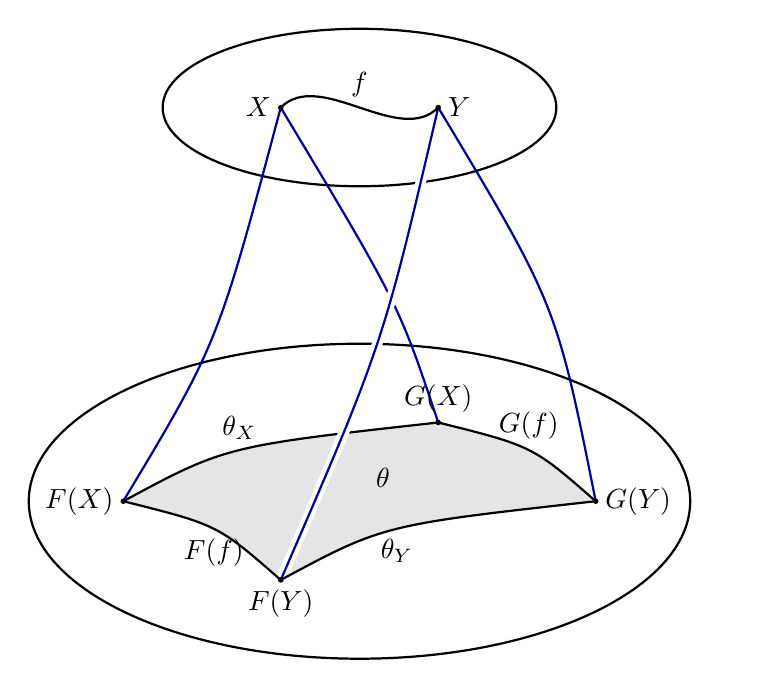
\begin{tikzpicture}
        \draw[thick] (0,3) ellipse (2.5 and 1)
        (0,-2) ellipse (4.2 and 2)
        node at (3, 3) {$\cC$}
        node at (4.7, -2) {$\cD$}
        coordinate (X) at (-1, 3)
        coordinate (Y) at (1, 3)
        coordinate (FX) at (-3, -2)
        coordinate (GY) at (3, -2)
        coordinate (GX) at (1, -1)
        coordinate (FY) at (-1, -3)
        coordinate (FX-GX-ct1) at (-1.7, -1.3)
        coordinate (FY-GY-ct1) at (0.3, -2.3)
        coordinate (FX-FY-ct1) at (-1.8, -2.3)
        coordinate (GX-GY-ct1) at (2.2, -1.3)
        coordinate (X-FX-ct1) at (-1.8, 0)
        coordinate (Y-FY-ct1) at (0.3, 0)
        coordinate (X-GX-ct1) at (0.5, 0.5)
        coordinate (Y-GY-ct1) at (2.5, 0.5);

        \fill[gray!20] (FX) .. controls (FX-GX-ct1) .. (GX) .. controls (GX-GY-ct1) .. (GY) .. controls (FY-GY-ct1) .. (FY) .. controls (FX-FY-ct1) .. (FX) -- cycle;

        \node at (0.3, -1.7) {$\theta$};

        \draw[thick] (FX) .. controls (FX-GX-ct1) .. node[above] {$\theta_X$} (GX) .. controls (GX-GY-ct1) .. node[above] {$G(f)$} (GY);
        \draw[thick,draw=blue!60!black] (X) .. controls (X-FX-ct1) .. (FX) (X) .. controls (X-GX-ct1) .. (GX);
        \draw[draw=white,double=blue!60!black,line width=1.5pt,double distance=0.8pt] (Y) .. controls (Y-FY-ct1) .. (FY);
        \draw[thick,draw=blue!60!black] (Y) .. controls (Y-GY-ct1) .. (GY);
        \draw[thick] (FX) .. controls (FX-FY-ct1) .. node[below] {$F(f)$} (FY) .. controls (FY-GY-ct1) .. node[below] {$\theta_Y$} (GY);
        \draw[thick] (X) .. controls (-.5, 3.5) and (.5, 2.5) .. node[above] {$f$} (Y);

        \node[left] at (X) {$X$};
        \node[right] at (Y) {$Y$};
        \node[left] at (FX) {$F(X)$};
        \node[right] at (GY) {$G(Y)$};
        \node[above] at (GX) {$G(X)$};
        \node[below] at (FY) {$F(Y)$};

        \foreach \point in {X, Y, FX, GX, GY, FY}
        \fill[black] (\point) circle (1pt);
    \end{tikzpicture}
    \caption{自然变换的几何直观}
    \label{fig:natural-transformation}
\end{figure}

首先,我们在一张纸上画两个面,表示两个范畴$\cC,\cD$. 在一个面上取两个点 $X, Y$,这是它上面的两个对象;然后,在另一个面上取四个点,分别表示 $F(X), F(Y), G(X), G(Y)$,即两个函子$F,G$在这两个点$X,Y$的取值. 注意,实际上两个函子分别是两个面之间的映射,如果把原像和像用线连接,展开来看的话,大概能看成是纸面上和纸面下的两张带有纹路的曲面. 然后,自然变换就是这两个曲面之间的连线$\theta$,对应到交换图上来,就是图中阴影区域的四条边. 实际上,我们的条件就是要求,这两族曲面$F, G$的结构和曲面之间的结构$\theta$都具备合适的连续性,如\autoref{fig:natural-transformation},这个东西在拓扑学中一般称为\term{同伦}.

在实践中,我们一般会称态射 $\theta_X$ 对于 $X$ 来说是自然的、典范的,或者说它满足函子性. 我们来看两个例子:

\begin{example}{}{}
    一个线性空间到某个商空间的投影映射. 考虑所有包含子空间 $U$ 的有限维线性空间. 显然,它们构成一个范畴,其间的态射定义为限制在 $U$ 上为恒同映射的线性映射,我们将这个东西记作 $\FVect_\F^U$.

    实际上,我们在说的是,考虑一个函子 $p\colon \FVect_\F^U \to \FVect_\F$ 将线性空间 $X$ 映到线性空间 $X/U$,另一个函子 $i\colon \FVect_\F^U \to \FVect_\F$ 将线性空间 $X$ 映到线性空间 $X$ 自身. 态射的映射都是显然的. 接下来,我们要表明存在一个自然变换 $\theta: i \to p$.

    现在,取任意的 $f\colon X \to Y$ 为 $\FVect_\F^U$ 中的态射,则我们需要使其交换的图表如下:

    \begin{center}
        \begin{tikzcd}
            X \rar["\theta_X"] \dar["f", swap] & X/U \dar["f/U"] \\
            Y \rar["\theta_Y", swap] & Y/U
        \end{tikzcd}
    \end{center}

    其中 $f/U$ 表示诱导的商映射,我们在不变子空间那一节中有所提及. 其中的 $\theta_X$ 和 $\theta_Y$ 就是我们通常称的典范投影,这也就是为什么这个投影被称为典范的.
\end{example}

下一个典范的结构我们也已经有所提及,它事关双对偶空间. 为了方便起见,对于函子 $F: \cC \to \cD$,我们记 $F^\mathrm{op}: \cC^\mathrm{op} \to \cD^\mathrm{op}$,它和原来的函子其实毫无差别,只有一点形式上的不同. 记对偶函子为 $-^*$,这是因为我们通常用 $V^*$ 表示对偶的空间,$f^*$ 表示对偶映射. 那么,我们就有 $(-^*)^\mathrm{op} \circ -^*$ 是典范同构. 这个事情的证明也是检查交换图,我们早已构造了这样的映射,也就是所谓的到双对偶空间的典范同构.

最后一个例子稍微有点特别,为了给出这个例子,我们需要定义一个与自然变换稍微有点不同的东西,强名之曰自然反变换\footnote{英文为 dinatural transformation,这个翻译稍微有点奇怪,但凑合用. }. 它的目标实际上是处理一些反变函子的情形,其它定义完全一致,不过它要求:$F: \cC \to \cD, G: \cC \to \cD^\mathrm{op}$,而它对应的交换图是:

\begin{center}
    \begin{tikzcd}
        F(X) \rar["\theta_X"] \dar["F(f)", swap] & G(X)\\
        F(Y) \rar["\theta_Y", swap] & G(Y) \uar["G(f)", swap]
    \end{tikzcd}
\end{center}

那么正如读者所料,我们要给出的结果就是:

\begin{example}{}{}
    不存在从一个线性空间到其对偶空间的非零自然反变换.

    现在,我们需要考虑下面的交换图:

    \begin{center}
        \begin{tikzcd}
            X \rar["\theta_X"] \dar["f", swap] & X^*\\
            Y \rar["\theta_Y", swap] & Y^* \uar["f^*", swap]
        \end{tikzcd}
    \end{center}

    我们知道,不管 $X$ 怎么取,总能取到一个 $f$ 使得 $f$ 将 $X$ 中的所有元素映到 $Y$ 中的零元,而参照我们的定义,这时的 $f^*$ 取值只有 $X^*$ 中的零元,因此,$\theta_X$ 为了让这个图交换,只能让所有元素映到零元.
\end{example}

可见在选取了合适的形式化方法之后,这些看上去无从下手的概念的证明变得无比单纯. 这实际上在表明,从一个空间到它的对偶空间不存在典范的同构.

\section{范畴论的构造}

单单是范畴、函子和自然变换显然什么都不能给出. 现在,我们无非是形式化了一些原来就已经说出的东西,顶多是最后对自然性的表述稍稍有些新意. 范畴论最核心的点实际上在于,它告诉了你很多被定义的东西实际上有其他的定义方式,这就是我们在这一节会讨论的内容.

\subsection{单态射、满态射和同构}

当我们在描述映射的时候,我们通常会讨论它是单的,满的,还是同构. 正如前面矩阵空间中关于指数映射的讨论中所表明的那样,这个性质实际上是非常不平凡的. 因此,这些性质应当在范畴论中得到恰当的推广——但是,时刻记住,现在我们的对象不同于以往我们做操作的集合,虽然我们还是能够从中汲取灵感.

先考虑集合的情况. 单射在我们看来,是如果像相同则原像相同,也就是说,每个原像集中的元素都有不同的像. 那么,就应当存在一个函数把它翻译回去,使得它在原像集上是恒同映射,也就是说:

\begin{lemma}{}{}
    考虑集合 $S, T$,一个函数 $f\colon T \to S$ 是单射当且仅当存在映射 $g\colon S \to T$ 使得 $g \circ f = \id_T$.
\end{lemma}

证明如上所述,形式化的写法留给读者,对偶地,我们就有:

\begin{lemma}{}{}
    $f\colon T \to S$ 是满射当且仅当存在映射 $g\colon S \to T$ 使得 $f \circ g = \id_S$.
\end{lemma}

而后面的这个定义是纯粹用箭头完成的,因此,它就能被推广到态射的情形:

\begin{definition}{}{}
    考虑范畴 $\cC$ 和其中的态射 $f\colon A \to B$.
    \begin{itemize}
        \item 称 $f$ 是\term{单态射},如果存在 $g\colon B \to A$ 使得 $g \circ f = \id_B$;
        \item 称 $f$ 是\term{满态射},如果存在 $g\colon B \to A$ 使得 $f \circ g = \id_A$;
        \item 称 $f$ 为\term{同构},如果存在 $g\colon B \to A$ 使得 $f \circ g = \id_A$ 且 $g \circ f = \id_B$;
        \item 如果 $A$ 和 $B$ 之间存在一个同构,则称 $A$ 和 $B$ 同构.
    \end{itemize}
\end{definition}

读者不难发现,恒同映射是一个同构. 这样的结构看上去就像一个逆元. 如果所有的态射都是同构,那么如果所有对象构成集合,态射也构成集合(这是为了避免一些集合论纷争),则我们将这个范畴构成一个\term{群胚}或者\term{广群}. 其态射集满足某种意义上的群结构. 实际上,在习题中我们会更进一步地发现相关的性质.

这里有一个麻烦的事情:同构一定既是单态射又是满态射,但既是单态射又是满态射的态射不一定是同构. 如果后者成立,则我们将这个范畴称为平衡范畴. 实际上,在通常的情形下,这个性质都是成立的.

\subsection{泛性质:始对象和终对象}

我们知道,一个范畴就是对象和箭头,那么,下面的定义看起来就很合乎情理:我们要选出箭头比较特殊的那些对象.

\begin{definition}{}{}
    称一个对象 $A \in \cC$ 为始对象,如果对于任意 $B \in \cC$ 都有 $|\Hom_\cC (A, B)| = 1$. 终对象是对偶范畴中的始对象. 如果一个对象既是始对象又是终对象,我们称其为零对象.
\end{definition}

注意,终对象的定义和始对象是完全对偶的,所以,很多时候我们其实不太区分这两种对象,它们具备的 $|\Hom_\cC (A, B)| = 1$ 的性质我们往往称为泛性质. 一般的,泛性质成立表明它实际上是一个定义性的东西:

\begin{theorem}{}{}
    所有始对象都是同构的、所有终对象都是同构的.
\end{theorem}

证明过于显然,留作读者练习. 重要的是例子:$\FVect$ 中,$\{1\}$ 是零对象. 这实际上说明了这个玩意的特殊性,但我们对它的特殊性早已习以为常. 剩下的一些例子我们会在后面的构造中一一给出——实际上,所有不太平凡的例子都要求我们构造一些更为奇特的范畴.

\subsection{Hom 函子和 Yoneda 引理}

注意到,如果 $\cC$ 和 $\cD$ 都是范畴,则 $\cC \times \cD$ 也是一个范畴,其上的对象和态射都是显然的. 我们首先考虑这样一个函子:
\[
    \Hom: \cC^\mathrm{op} \times \cC \to \Set
\]

它将对象 $(c, c')$ 映到它们之间的态射集 $\Hom_\cC(c, c')$,而将态射 $(f: c \leftarrow d, f': c' \to d')$ 映到一个 $\Hom_\cC(c, c') \to \Hom_\cC(d, d')$ 的映射,以复合的形式:
\[
    \Hom(f, f')(q: c \to c') = f' \circ q \circ f
\]

这个东西看起来乌七八糟的,但是在后面谈到张量积的时候,这个定义会体现出一个非常明显的性质. 在此,我们考虑另一种

\subsection{伴随函子}

\subsection{逗号范畴}

\subsection{和与积、极限和余极限}

\subsection{纤维化和余纤维化}

\section{幺半范畴及其性质}

\subsection{函子范畴和单子}

\subsection{Beck 单子化定理*}

\subsection{张量积}

\section{2-范畴一瞥}

\subsection{伴随和伴随}

\subsection{作为 2-极限的逗号范畴}

\subsection{走向无穷范畴:为什么我们需要套娃?}

\begin{exercise}
    \exquote[——《收获与播种》,格罗滕迪克]{每一门科学,当我们不是将它作为能力和统治力的工具,而是作为我们人类世代以来努力追求的对知识的冒险历程,不是别的,就是这样一种和谐,从一个时期到另一个时期,或多或少,巨大而又丰富:在不同的时代和世纪中,对于依次出现的不同的主题,它展现给我们微妙而精细的对应,仿佛来自虚空。}

    \begin{enumerate}  % 若不需要编号,则直接使用 enumerate 环境
        \item 证明以下两个态射的性质:
        \begin{enumerate}
            \item 如果 $A$ 与 $B$ 同构,那么 $A$ 与 $B$ 之间的同构映射是唯一的;
            \item 函子保持态射的单、满性质.
        \end{enumerate}
    \end{enumerate}
\end{exercise}


\LUgroupsancheck

\makeatletter
\let\chapter\@std@chapter
\let\@std@chapter\relax
\makeatother

\backmatter
{\small
\printindex
\printindex[sym]
}

\end{document}
